\documentclass[twoside]{book}

% Packages required by doxygen
\usepackage{fixltx2e}
\usepackage{calc}
\usepackage{doxygen}
\usepackage[export]{adjustbox} % also loads graphicx
\usepackage{graphicx}
\usepackage[utf8]{inputenc}
\usepackage{makeidx}
\usepackage{multicol}
\usepackage{multirow}
\PassOptionsToPackage{warn}{textcomp}
\usepackage{textcomp}
\usepackage[nointegrals]{wasysym}
\usepackage[table]{xcolor}

% Font selection
\usepackage[T1]{fontenc}
\usepackage[scaled=.90]{helvet}
\usepackage{courier}
\usepackage{amssymb}
\usepackage{sectsty}
\renewcommand{\familydefault}{\sfdefault}
\allsectionsfont{%
  \fontseries{bc}\selectfont%
  \color{darkgray}%
}
\renewcommand{\DoxyLabelFont}{%
  \fontseries{bc}\selectfont%
  \color{darkgray}%
}
\newcommand{\+}{\discretionary{\mbox{\scriptsize$\hookleftarrow$}}{}{}}

% Page & text layout
\usepackage{geometry}
\geometry{%
  a4paper,%
  top=2.5cm,%
  bottom=2.5cm,%
  left=2.5cm,%
  right=2.5cm%
}
\tolerance=750
\hfuzz=15pt
\hbadness=750
\setlength{\emergencystretch}{15pt}
\setlength{\parindent}{0cm}
\setlength{\parskip}{3ex plus 2ex minus 2ex}
\makeatletter
\renewcommand{\paragraph}{%
  \@startsection{paragraph}{4}{0ex}{-1.0ex}{1.0ex}{%
    \normalfont\normalsize\bfseries\SS@parafont%
  }%
}
\renewcommand{\subparagraph}{%
  \@startsection{subparagraph}{5}{0ex}{-1.0ex}{1.0ex}{%
    \normalfont\normalsize\bfseries\SS@subparafont%
  }%
}
\makeatother

% Headers & footers
\usepackage{fancyhdr}
\pagestyle{fancyplain}
\fancyhead[LE]{\fancyplain{}{\bfseries\thepage}}
\fancyhead[CE]{\fancyplain{}{}}
\fancyhead[RE]{\fancyplain{}{\bfseries\leftmark}}
\fancyhead[LO]{\fancyplain{}{\bfseries\rightmark}}
\fancyhead[CO]{\fancyplain{}{}}
\fancyhead[RO]{\fancyplain{}{\bfseries\thepage}}
\fancyfoot[LE]{\fancyplain{}{}}
\fancyfoot[CE]{\fancyplain{}{}}
\fancyfoot[RE]{\fancyplain{}{\bfseries\scriptsize Generated by Doxygen }}
\fancyfoot[LO]{\fancyplain{}{\bfseries\scriptsize Generated by Doxygen }}
\fancyfoot[CO]{\fancyplain{}{}}
\fancyfoot[RO]{\fancyplain{}{}}
\renewcommand{\footrulewidth}{0.4pt}
\renewcommand{\chaptermark}[1]{%
  \markboth{#1}{}%
}
\renewcommand{\sectionmark}[1]{%
  \markright{\thesection\ #1}%
}

% Indices & bibliography
\usepackage{natbib}
\usepackage[titles]{tocloft}
\setcounter{tocdepth}{3}
\setcounter{secnumdepth}{5}
\makeindex

% Hyperlinks (required, but should be loaded last)
\usepackage{ifpdf}
\ifpdf
  \usepackage[pdftex,pagebackref=true]{hyperref}
\else
  \usepackage[ps2pdf,pagebackref=true]{hyperref}
\fi
\hypersetup{%
  colorlinks=true,%
  linkcolor=blue,%
  citecolor=blue,%
  unicode%
}

% Custom commands
\newcommand{\clearemptydoublepage}{%
  \newpage{\pagestyle{empty}\cleardoublepage}%
}

\usepackage{caption}
\captionsetup{labelsep=space,justification=centering,font={bf},singlelinecheck=off,skip=4pt,position=top}

%===== C O N T E N T S =====

\begin{document}

% Titlepage & ToC
\hypersetup{pageanchor=false,
             bookmarksnumbered=true,
             pdfencoding=unicode
            }
\pagenumbering{alph}
\begin{titlepage}
\vspace*{7cm}
\begin{center}%
{\Large Redis-\/\+Quant365 }\\
\vspace*{1cm}
{\large Generated by Doxygen 1.8.13}\\
\end{center}
\end{titlepage}
\clearemptydoublepage
\pagenumbering{roman}
\tableofcontents
\clearemptydoublepage
\pagenumbering{arabic}
\hypersetup{pageanchor=true}

%--- Begin generated contents ---
\chapter{Data Structure Index}
\section{Data Structures}
Here are the data structures with brief descriptions\+:\begin{DoxyCompactList}
\item\contentsline{section}{\hyperlink{struct__client}{\+\_\+client} }{\pageref{struct__client}}{}
\item\contentsline{section}{\hyperlink{unionzsetopsrc_1_1__iterset_8iter_8set}{\+\_\+iterset.\+iter.\+set} }{\pageref{unionzsetopsrc_1_1__iterset_8iter_8set}}{}
\item\contentsline{section}{\hyperlink{structzsetopsrc_1_1__iterset_8iter_8set_8ht}{\+\_\+iterset.\+iter.\+set.\+ht} }{\pageref{structzsetopsrc_1_1__iterset_8iter_8set_8ht}}{}
\item\contentsline{section}{\hyperlink{structzsetopsrc_1_1__iterset_8iter_8set_8is}{\+\_\+iterset.\+iter.\+set.\+is} }{\pageref{structzsetopsrc_1_1__iterset_8iter_8set_8is}}{}
\item\contentsline{section}{\hyperlink{unionzsetopsrc_1_1__iterzset_8iter_8zset}{\+\_\+iterzset.\+iter.\+zset} }{\pageref{unionzsetopsrc_1_1__iterzset_8iter_8zset}}{}
\item\contentsline{section}{\hyperlink{structzsetopsrc_1_1__iterzset_8iter_8zset_8sl}{\+\_\+iterzset.\+iter.\+zset.\+sl} }{\pageref{structzsetopsrc_1_1__iterzset_8iter_8zset_8sl}}{}
\item\contentsline{section}{\hyperlink{structzsetopsrc_1_1__iterzset_8iter_8zset_8zl}{\+\_\+iterzset.\+iter.\+zset.\+zl} }{\pageref{structzsetopsrc_1_1__iterzset_8iter_8zset_8zl}}{}
\item\contentsline{section}{\hyperlink{struct__redisSortObject}{\+\_\+redis\+Sort\+Object} }{\pageref{struct__redisSortObject}}{}
\item\contentsline{section}{\hyperlink{union__redisSortObject_8u}{\+\_\+redis\+Sort\+Object.\+u} }{\pageref{union__redisSortObject_8u}}{}
\item\contentsline{section}{\hyperlink{struct__redisSortOperation}{\+\_\+redis\+Sort\+Operation} }{\pageref{struct__redisSortOperation}}{}
\item\contentsline{section}{\hyperlink{struct__rio}{\+\_\+rio} }{\pageref{struct__rio}}{}
\item\contentsline{section}{\hyperlink{union__rio_8io}{\+\_\+rio.\+io} }{\pageref{union__rio_8io}}{}
\item\contentsline{section}{\hyperlink{struct__rio_8io_8buffer}{\+\_\+rio.\+io.\+buffer} }{\pageref{struct__rio_8io_8buffer}}{}
\item\contentsline{section}{\hyperlink{struct__rio_8io_8fdset}{\+\_\+rio.\+io.\+fdset} }{\pageref{struct__rio_8io_8fdset}}{}
\item\contentsline{section}{\hyperlink{struct__rio_8io_8file}{\+\_\+rio.\+io.\+file} }{\pageref{struct__rio_8io_8file}}{}
\item\contentsline{section}{\hyperlink{structaeApiState}{ae\+Api\+State} }{\pageref{structaeApiState}}{}
\item\contentsline{section}{\hyperlink{structaeEventLoop}{ae\+Event\+Loop} }{\pageref{structaeEventLoop}}{}
\item\contentsline{section}{\hyperlink{structaeFileEvent}{ae\+File\+Event} }{\pageref{structaeFileEvent}}{}
\item\contentsline{section}{\hyperlink{structaeFiredEvent}{ae\+Fired\+Event} }{\pageref{structaeFiredEvent}}{}
\item\contentsline{section}{\hyperlink{structaeTimeEvent}{ae\+Time\+Event} }{\pageref{structaeTimeEvent}}{}
\item\contentsline{section}{\hyperlink{structaofrwblock}{aofrwblock} }{\pageref{structaofrwblock}}{}
\item\contentsline{section}{\hyperlink{structAutoMemEntry}{Auto\+Mem\+Entry} }{\pageref{structAutoMemEntry}}{}
\item\contentsline{section}{\hyperlink{structbio__job}{bio\+\_\+job} }{\pageref{structbio__job}}{}
\item\contentsline{section}{\hyperlink{structbitfieldOp}{bitfield\+Op} }{\pageref{structbitfieldOp}}{}
\item\contentsline{section}{\hyperlink{structblockingState}{blocking\+State} }{\pageref{structblockingState}}{}
\item\contentsline{section}{\hyperlink{structclient}{client} }{\pageref{structclient}}{}
\item\contentsline{section}{\hyperlink{structclientBufferLimitsConfig}{client\+Buffer\+Limits\+Config} }{\pageref{structclientBufferLimitsConfig}}{}
\item\contentsline{section}{\hyperlink{structclusterLink}{cluster\+Link} }{\pageref{structclusterLink}}{}
\item\contentsline{section}{\hyperlink{structclusterMsg}{cluster\+Msg} }{\pageref{structclusterMsg}}{}
\item\contentsline{section}{\hyperlink{unionclusterMsgData}{cluster\+Msg\+Data} }{\pageref{unionclusterMsgData}}{}
\item\contentsline{section}{\hyperlink{structclusterMsgData_8fail}{cluster\+Msg\+Data.\+fail} }{\pageref{structclusterMsgData_8fail}}{}
\item\contentsline{section}{\hyperlink{structclusterMsgData_8ping}{cluster\+Msg\+Data.\+ping} }{\pageref{structclusterMsgData_8ping}}{}
\item\contentsline{section}{\hyperlink{structclusterMsgData_8publish}{cluster\+Msg\+Data.\+publish} }{\pageref{structclusterMsgData_8publish}}{}
\item\contentsline{section}{\hyperlink{structclusterMsgData_8update}{cluster\+Msg\+Data.\+update} }{\pageref{structclusterMsgData_8update}}{}
\item\contentsline{section}{\hyperlink{structclusterMsgDataFail}{cluster\+Msg\+Data\+Fail} }{\pageref{structclusterMsgDataFail}}{}
\item\contentsline{section}{\hyperlink{structclusterMsgDataGossip}{cluster\+Msg\+Data\+Gossip} }{\pageref{structclusterMsgDataGossip}}{}
\item\contentsline{section}{\hyperlink{structclusterMsgDataPublish}{cluster\+Msg\+Data\+Publish} }{\pageref{structclusterMsgDataPublish}}{}
\item\contentsline{section}{\hyperlink{structclusterMsgDataUpdate}{cluster\+Msg\+Data\+Update} }{\pageref{structclusterMsgDataUpdate}}{}
\item\contentsline{section}{\hyperlink{structclusterNode}{cluster\+Node} }{\pageref{structclusterNode}}{}
\item\contentsline{section}{\hyperlink{structclusterNodeFailReport}{cluster\+Node\+Fail\+Report} }{\pageref{structclusterNodeFailReport}}{}
\item\contentsline{section}{\hyperlink{structclusterState}{cluster\+State} }{\pageref{structclusterState}}{}
\item\contentsline{section}{\hyperlink{structcommandHelp}{command\+Help} }{\pageref{structcommandHelp}}{}
\item\contentsline{section}{\hyperlink{structconfigEnum}{config\+Enum} }{\pageref{structconfigEnum}}{}
\item\contentsline{section}{\hyperlink{structdict}{dict} }{\pageref{structdict}}{}
\item\contentsline{section}{\hyperlink{structdictEntry}{dict\+Entry} }{\pageref{structdictEntry}}{}
\item\contentsline{section}{\hyperlink{uniondictEntry_8v}{dict\+Entry.\+v} }{\pageref{uniondictEntry_8v}}{}
\item\contentsline{section}{\hyperlink{structdictht}{dictht} }{\pageref{structdictht}}{}
\item\contentsline{section}{\hyperlink{structdictIterator}{dict\+Iterator} }{\pageref{structdictIterator}}{}
\item\contentsline{section}{\hyperlink{structdictType}{dict\+Type} }{\pageref{structdictType}}{}
\item\contentsline{section}{\hyperlink{structdistsamples}{distsamples} }{\pageref{structdistsamples}}{}
\item\contentsline{section}{\hyperlink{structevictionPoolEntry}{eviction\+Pool\+Entry} }{\pageref{structevictionPoolEntry}}{}
\item\contentsline{section}{\hyperlink{structgeoArray}{geo\+Array} }{\pageref{structgeoArray}}{}
\item\contentsline{section}{\hyperlink{structGeoHashArea}{Geo\+Hash\+Area} }{\pageref{structGeoHashArea}}{}
\item\contentsline{section}{\hyperlink{structGeoHashBits}{Geo\+Hash\+Bits} }{\pageref{structGeoHashBits}}{}
\item\contentsline{section}{\hyperlink{structGeoHashNeighbors}{Geo\+Hash\+Neighbors} }{\pageref{structGeoHashNeighbors}}{}
\item\contentsline{section}{\hyperlink{structGeoHashRadius}{Geo\+Hash\+Radius} }{\pageref{structGeoHashRadius}}{}
\item\contentsline{section}{\hyperlink{structGeoHashRange}{Geo\+Hash\+Range} }{\pageref{structGeoHashRange}}{}
\item\contentsline{section}{\hyperlink{structgeoPoint}{geo\+Point} }{\pageref{structgeoPoint}}{}
\item\contentsline{section}{\hyperlink{structhashTypeIterator}{hash\+Type\+Iterator} }{\pageref{structhashTypeIterator}}{}
\item\contentsline{section}{\hyperlink{structHelloTypeNode}{Hello\+Type\+Node} }{\pageref{structHelloTypeNode}}{}
\item\contentsline{section}{\hyperlink{structHelloTypeObject}{Hello\+Type\+Object} }{\pageref{structHelloTypeObject}}{}
\item\contentsline{section}{\hyperlink{structhelpEntry}{help\+Entry} }{\pageref{structhelpEntry}}{}
\item\contentsline{section}{\hyperlink{structhllhdr}{hllhdr} }{\pageref{structhllhdr}}{}
\item\contentsline{section}{\hyperlink{structinstanceLink}{instance\+Link} }{\pageref{structinstanceLink}}{}
\item\contentsline{section}{\hyperlink{structintset}{intset} }{\pageref{structintset}}{}
\item\contentsline{section}{\hyperlink{structlatencySample}{latency\+Sample} }{\pageref{structlatencySample}}{}
\item\contentsline{section}{\hyperlink{structlatencyStats}{latency\+Stats} }{\pageref{structlatencyStats}}{}
\item\contentsline{section}{\hyperlink{structlatencyTimeSeries}{latency\+Time\+Series} }{\pageref{structlatencyTimeSeries}}{}
\item\contentsline{section}{\hyperlink{structldbState}{ldb\+State} }{\pageref{structldbState}}{}
\item\contentsline{section}{\hyperlink{structlist}{list} }{\pageref{structlist}}{}
\item\contentsline{section}{\hyperlink{structlistIter}{list\+Iter} }{\pageref{structlistIter}}{}
\item\contentsline{section}{\hyperlink{structlistNode}{list\+Node} }{\pageref{structlistNode}}{}
\item\contentsline{section}{\hyperlink{structlistTypeEntry}{list\+Type\+Entry} }{\pageref{structlistTypeEntry}}{}
\item\contentsline{section}{\hyperlink{structlistTypeIterator}{list\+Type\+Iterator} }{\pageref{structlistTypeIterator}}{}
\item\contentsline{section}{\hyperlink{structmigrateCachedSocket}{migrate\+Cached\+Socket} }{\pageref{structmigrateCachedSocket}}{}
\item\contentsline{section}{\hyperlink{structmoduleLoadQueueEntry}{module\+Load\+Queue\+Entry} }{\pageref{structmoduleLoadQueueEntry}}{}
\item\contentsline{section}{\hyperlink{structmoduleValue}{module\+Value} }{\pageref{structmoduleValue}}{}
\item\contentsline{section}{\hyperlink{structmultiCmd}{multi\+Cmd} }{\pageref{structmultiCmd}}{}
\item\contentsline{section}{\hyperlink{structmultiState}{multi\+State} }{\pageref{structmultiState}}{}
\item\contentsline{section}{\hyperlink{structpubsubPattern}{pubsub\+Pattern} }{\pageref{structpubsubPattern}}{}
\item\contentsline{section}{\hyperlink{structquicklist}{quicklist} }{\pageref{structquicklist}}{}
\item\contentsline{section}{\hyperlink{structquicklistEntry}{quicklist\+Entry} }{\pageref{structquicklistEntry}}{}
\item\contentsline{section}{\hyperlink{structquicklistIter}{quicklist\+Iter} }{\pageref{structquicklistIter}}{}
\item\contentsline{section}{\hyperlink{structquicklistLZF}{quicklist\+L\+ZF} }{\pageref{structquicklistLZF}}{}
\item\contentsline{section}{\hyperlink{structquicklistNode}{quicklist\+Node} }{\pageref{structquicklistNode}}{}
\item\contentsline{section}{\hyperlink{structrax}{rax} }{\pageref{structrax}}{}
\item\contentsline{section}{\hyperlink{structraxIterator}{rax\+Iterator} }{\pageref{structraxIterator}}{}
\item\contentsline{section}{\hyperlink{structraxNode}{rax\+Node} }{\pageref{structraxNode}}{}
\item\contentsline{section}{\hyperlink{structraxStack}{rax\+Stack} }{\pageref{structraxStack}}{}
\item\contentsline{section}{\hyperlink{structrdbSaveInfo}{rdb\+Save\+Info} }{\pageref{structrdbSaveInfo}}{}
\item\contentsline{section}{\hyperlink{structreadyList}{ready\+List} }{\pageref{structreadyList}}{}
\item\contentsline{section}{\hyperlink{structredisAeEvents}{redis\+Ae\+Events} }{\pageref{structredisAeEvents}}{}
\item\contentsline{section}{\hyperlink{structredisCommand}{redis\+Command} }{\pageref{structredisCommand}}{}
\item\contentsline{section}{\hyperlink{structredisDb}{redis\+Db} }{\pageref{structredisDb}}{}
\item\contentsline{section}{\hyperlink{structredisFunctionSym}{redis\+Function\+Sym} }{\pageref{structredisFunctionSym}}{}
\item\contentsline{section}{\hyperlink{structredisMemOverhead}{redis\+Mem\+Overhead} }{\pageref{structredisMemOverhead}}{}
\item\contentsline{section}{\hyperlink{structredisMemOverhead_8db}{redis\+Mem\+Overhead.\+db} }{\pageref{structredisMemOverhead_8db}}{}
\item\contentsline{section}{\hyperlink{structRedisModule}{Redis\+Module} }{\pageref{structRedisModule}}{}
\item\contentsline{section}{\hyperlink{structRedisModuleBlockedClient}{Redis\+Module\+Blocked\+Client} }{\pageref{structRedisModuleBlockedClient}}{}
\item\contentsline{section}{\hyperlink{structRedisModuleCallReply}{Redis\+Module\+Call\+Reply} }{\pageref{structRedisModuleCallReply}}{}
\item\contentsline{section}{\hyperlink{unionRedisModuleCallReply_8val}{Redis\+Module\+Call\+Reply.\+val} }{\pageref{unionRedisModuleCallReply_8val}}{}
\item\contentsline{section}{\hyperlink{structRedisModuleCommandProxy}{Redis\+Module\+Command\+Proxy} }{\pageref{structRedisModuleCommandProxy}}{}
\item\contentsline{section}{\hyperlink{structRedisModuleCtx}{Redis\+Module\+Ctx} }{\pageref{structRedisModuleCtx}}{}
\item\contentsline{section}{\hyperlink{structRedisModuleDigest}{Redis\+Module\+Digest} }{\pageref{structRedisModuleDigest}}{}
\item\contentsline{section}{\hyperlink{structRedisModuleIO}{Redis\+Module\+IO} }{\pageref{structRedisModuleIO}}{}
\item\contentsline{section}{\hyperlink{structRedisModuleKey}{Redis\+Module\+Key} }{\pageref{structRedisModuleKey}}{}
\item\contentsline{section}{\hyperlink{structRedisModulePoolAllocBlock}{Redis\+Module\+Pool\+Alloc\+Block} }{\pageref{structRedisModulePoolAllocBlock}}{}
\item\contentsline{section}{\hyperlink{structRedisModuleType}{Redis\+Module\+Type} }{\pageref{structRedisModuleType}}{}
\item\contentsline{section}{\hyperlink{structRedisModuleTypeMethods}{Redis\+Module\+Type\+Methods} }{\pageref{structRedisModuleTypeMethods}}{}
\item\contentsline{section}{\hyperlink{structredisNodeFlags}{redis\+Node\+Flags} }{\pageref{structredisNodeFlags}}{}
\item\contentsline{section}{\hyperlink{structredisObject}{redis\+Object} }{\pageref{structredisObject}}{}
\item\contentsline{section}{\hyperlink{structredisOp}{redis\+Op} }{\pageref{structredisOp}}{}
\item\contentsline{section}{\hyperlink{structredisOpArray}{redis\+Op\+Array} }{\pageref{structredisOpArray}}{}
\item\contentsline{section}{\hyperlink{structredisServer}{redis\+Server} }{\pageref{structredisServer}}{}
\item\contentsline{section}{\hyperlink{structredisServer_8child__info__data}{redis\+Server.\+child\+\_\+info\+\_\+data} }{\pageref{structredisServer_8child__info__data}}{}
\item\contentsline{section}{\hyperlink{structredisServer_8inst__metric}{redis\+Server.\+inst\+\_\+metric} }{\pageref{structredisServer_8inst__metric}}{}
\item\contentsline{section}{\hyperlink{structsample}{sample} }{\pageref{structsample}}{}
\item\contentsline{section}{\hyperlink{structsaveparam}{saveparam} }{\pageref{structsaveparam}}{}
\item\contentsline{section}{\hyperlink{structsentinelAddr}{sentinel\+Addr} }{\pageref{structsentinelAddr}}{}
\item\contentsline{section}{\hyperlink{structsentinelLeader}{sentinel\+Leader} }{\pageref{structsentinelLeader}}{}
\item\contentsline{section}{\hyperlink{structsentinelRedisInstance}{sentinel\+Redis\+Instance} }{\pageref{structsentinelRedisInstance}}{}
\item\contentsline{section}{\hyperlink{structsentinelScriptJob}{sentinel\+Script\+Job} }{\pageref{structsentinelScriptJob}}{}
\item\contentsline{section}{\hyperlink{structsentinelState}{sentinel\+State} }{\pageref{structsentinelState}}{}
\item\contentsline{section}{\hyperlink{structsequence}{sequence} }{\pageref{structsequence}}{}
\item\contentsline{section}{\hyperlink{structsetTypeIterator}{set\+Type\+Iterator} }{\pageref{structsetTypeIterator}}{}
\item\contentsline{section}{\hyperlink{structSHA1__CTX}{S\+H\+A1\+\_\+\+C\+TX} }{\pageref{structSHA1__CTX}}{}
\item\contentsline{section}{\hyperlink{structsharedObjectsStruct}{shared\+Objects\+Struct} }{\pageref{structsharedObjectsStruct}}{}
\item\contentsline{section}{\hyperlink{structslowlogEntry}{slowlog\+Entry} }{\pageref{structslowlogEntry}}{}
\item\contentsline{section}{\hyperlink{structstream}{stream} }{\pageref{structstream}}{}
\item\contentsline{section}{\hyperlink{structstreamID}{stream\+ID} }{\pageref{structstreamID}}{}
\item\contentsline{section}{\hyperlink{structstreamIterator}{stream\+Iterator} }{\pageref{structstreamIterator}}{}
\item\contentsline{section}{\hyperlink{structwatchedKey}{watched\+Key} }{\pageref{structwatchedKey}}{}
\item\contentsline{section}{\hyperlink{structzlentry}{zlentry} }{\pageref{structzlentry}}{}
\item\contentsline{section}{\hyperlink{structzlexrangespec}{zlexrangespec} }{\pageref{structzlexrangespec}}{}
\item\contentsline{section}{\hyperlink{structzrangespec}{zrangespec} }{\pageref{structzrangespec}}{}
\item\contentsline{section}{\hyperlink{structzset}{zset} }{\pageref{structzset}}{}
\item\contentsline{section}{\hyperlink{structzsetopsrc}{zsetopsrc} }{\pageref{structzsetopsrc}}{}
\item\contentsline{section}{\hyperlink{unionzsetopsrc_8iter}{zsetopsrc.\+iter} }{\pageref{unionzsetopsrc_8iter}}{}
\item\contentsline{section}{\hyperlink{structzsetopval}{zsetopval} }{\pageref{structzsetopval}}{}
\item\contentsline{section}{\hyperlink{structzskiplist}{zskiplist} }{\pageref{structzskiplist}}{}
\item\contentsline{section}{\hyperlink{structzskiplistNode}{zskiplist\+Node} }{\pageref{structzskiplistNode}}{}
\end{DoxyCompactList}

\chapter{Data Structure Documentation}
\hypertarget{struct__client}{}\section{\+\_\+client Struct Reference}
\label{struct__client}\index{\+\_\+client@{\+\_\+client}}


Collaboration diagram for \+\_\+client\+:\nopagebreak
\begin{figure}[H]
\begin{center}
\leavevmode
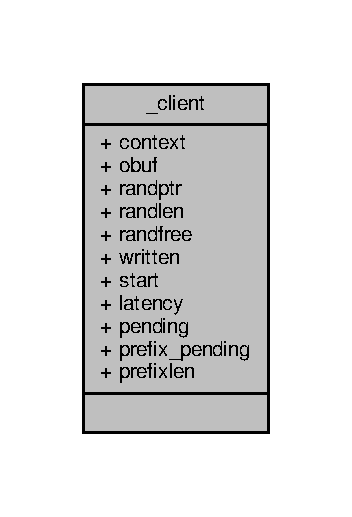
\includegraphics[width=169pt]{struct__client__coll__graph}
\end{center}
\end{figure}
\subsection*{Data Fields}
\begin{DoxyCompactItemize}
\item 
\mbox{\Hypertarget{struct__client_a2180e6fe84ab03b7ba66cc1a042c8dce}\label{struct__client_a2180e6fe84ab03b7ba66cc1a042c8dce}} 
redis\+Context $\ast$ {\bfseries context}
\item 
\mbox{\Hypertarget{struct__client_adeff017bf03ed263e419459cd77f54bf}\label{struct__client_adeff017bf03ed263e419459cd77f54bf}} 
sds {\bfseries obuf}
\item 
\mbox{\Hypertarget{struct__client_ac87622a714444d3ebbe429c468c579ff}\label{struct__client_ac87622a714444d3ebbe429c468c579ff}} 
char $\ast$$\ast$ {\bfseries randptr}
\item 
\mbox{\Hypertarget{struct__client_a60cb677f41011ed39ef369bdee286717}\label{struct__client_a60cb677f41011ed39ef369bdee286717}} 
size\+\_\+t {\bfseries randlen}
\item 
\mbox{\Hypertarget{struct__client_a17e1e70f120c1b211d0f374617a9e269}\label{struct__client_a17e1e70f120c1b211d0f374617a9e269}} 
size\+\_\+t {\bfseries randfree}
\item 
\mbox{\Hypertarget{struct__client_a09708e74a9931a2fd4fc74192c1e6c45}\label{struct__client_a09708e74a9931a2fd4fc74192c1e6c45}} 
size\+\_\+t {\bfseries written}
\item 
\mbox{\Hypertarget{struct__client_a446ec52a7b7272d00f0e8078180bfe70}\label{struct__client_a446ec52a7b7272d00f0e8078180bfe70}} 
long long {\bfseries start}
\item 
\mbox{\Hypertarget{struct__client_ad9cf812e88222e91e13a67879941d0aa}\label{struct__client_ad9cf812e88222e91e13a67879941d0aa}} 
long long {\bfseries latency}
\item 
\mbox{\Hypertarget{struct__client_a5eac5d96479e9f8ab90b354091ba52b2}\label{struct__client_a5eac5d96479e9f8ab90b354091ba52b2}} 
int {\bfseries pending}
\item 
\mbox{\Hypertarget{struct__client_aad427d69d85dfc467667d98db731fbf6}\label{struct__client_aad427d69d85dfc467667d98db731fbf6}} 
int {\bfseries prefix\+\_\+pending}
\item 
\mbox{\Hypertarget{struct__client_aa41fe19a482f33556cd423d41edff795}\label{struct__client_aa41fe19a482f33556cd423d41edff795}} 
int {\bfseries prefixlen}
\end{DoxyCompactItemize}


\subsection{Detailed Description}


Definition at line \hyperlink{redis-benchmark_8c_source_l00084}{84} of file \hyperlink{redis-benchmark_8c_source}{redis-\/benchmark.\+c}.



\subsection{Field Documentation}
\mbox{\Hypertarget{struct__client_a2180e6fe84ab03b7ba66cc1a042c8dce}\label{struct__client_a2180e6fe84ab03b7ba66cc1a042c8dce}} 
\index{\+\_\+client@{\+\_\+client}!context@{context}}
\index{context@{context}!\+\_\+client@{\+\_\+client}}
\subsubsection{\texorpdfstring{context}{context}}
{\footnotesize\ttfamily redis\+Context$\ast$ \+\_\+client\+::context}



Definition at line \hyperlink{redis-benchmark_8c_source_l00085}{85} of file \hyperlink{redis-benchmark_8c_source}{redis-\/benchmark.\+c}.

\mbox{\Hypertarget{struct__client_ad9cf812e88222e91e13a67879941d0aa}\label{struct__client_ad9cf812e88222e91e13a67879941d0aa}} 
\index{\+\_\+client@{\+\_\+client}!latency@{latency}}
\index{latency@{latency}!\+\_\+client@{\+\_\+client}}
\subsubsection{\texorpdfstring{latency}{latency}}
{\footnotesize\ttfamily long long \+\_\+client\+::latency}



Definition at line \hyperlink{redis-benchmark_8c_source_l00092}{92} of file \hyperlink{redis-benchmark_8c_source}{redis-\/benchmark.\+c}.

\mbox{\Hypertarget{struct__client_adeff017bf03ed263e419459cd77f54bf}\label{struct__client_adeff017bf03ed263e419459cd77f54bf}} 
\index{\+\_\+client@{\+\_\+client}!obuf@{obuf}}
\index{obuf@{obuf}!\+\_\+client@{\+\_\+client}}
\subsubsection{\texorpdfstring{obuf}{obuf}}
{\footnotesize\ttfamily sds \+\_\+client\+::obuf}



Definition at line \hyperlink{redis-benchmark_8c_source_l00086}{86} of file \hyperlink{redis-benchmark_8c_source}{redis-\/benchmark.\+c}.

\mbox{\Hypertarget{struct__client_a5eac5d96479e9f8ab90b354091ba52b2}\label{struct__client_a5eac5d96479e9f8ab90b354091ba52b2}} 
\index{\+\_\+client@{\+\_\+client}!pending@{pending}}
\index{pending@{pending}!\+\_\+client@{\+\_\+client}}
\subsubsection{\texorpdfstring{pending}{pending}}
{\footnotesize\ttfamily int \+\_\+client\+::pending}



Definition at line \hyperlink{redis-benchmark_8c_source_l00093}{93} of file \hyperlink{redis-benchmark_8c_source}{redis-\/benchmark.\+c}.

\mbox{\Hypertarget{struct__client_aad427d69d85dfc467667d98db731fbf6}\label{struct__client_aad427d69d85dfc467667d98db731fbf6}} 
\index{\+\_\+client@{\+\_\+client}!prefix\+\_\+pending@{prefix\+\_\+pending}}
\index{prefix\+\_\+pending@{prefix\+\_\+pending}!\+\_\+client@{\+\_\+client}}
\subsubsection{\texorpdfstring{prefix\+\_\+pending}{prefix\_pending}}
{\footnotesize\ttfamily int \+\_\+client\+::prefix\+\_\+pending}



Definition at line \hyperlink{redis-benchmark_8c_source_l00094}{94} of file \hyperlink{redis-benchmark_8c_source}{redis-\/benchmark.\+c}.

\mbox{\Hypertarget{struct__client_aa41fe19a482f33556cd423d41edff795}\label{struct__client_aa41fe19a482f33556cd423d41edff795}} 
\index{\+\_\+client@{\+\_\+client}!prefixlen@{prefixlen}}
\index{prefixlen@{prefixlen}!\+\_\+client@{\+\_\+client}}
\subsubsection{\texorpdfstring{prefixlen}{prefixlen}}
{\footnotesize\ttfamily int \+\_\+client\+::prefixlen}



Definition at line \hyperlink{redis-benchmark_8c_source_l00097}{97} of file \hyperlink{redis-benchmark_8c_source}{redis-\/benchmark.\+c}.

\mbox{\Hypertarget{struct__client_a17e1e70f120c1b211d0f374617a9e269}\label{struct__client_a17e1e70f120c1b211d0f374617a9e269}} 
\index{\+\_\+client@{\+\_\+client}!randfree@{randfree}}
\index{randfree@{randfree}!\+\_\+client@{\+\_\+client}}
\subsubsection{\texorpdfstring{randfree}{randfree}}
{\footnotesize\ttfamily size\+\_\+t \+\_\+client\+::randfree}



Definition at line \hyperlink{redis-benchmark_8c_source_l00089}{89} of file \hyperlink{redis-benchmark_8c_source}{redis-\/benchmark.\+c}.

\mbox{\Hypertarget{struct__client_a60cb677f41011ed39ef369bdee286717}\label{struct__client_a60cb677f41011ed39ef369bdee286717}} 
\index{\+\_\+client@{\+\_\+client}!randlen@{randlen}}
\index{randlen@{randlen}!\+\_\+client@{\+\_\+client}}
\subsubsection{\texorpdfstring{randlen}{randlen}}
{\footnotesize\ttfamily size\+\_\+t \+\_\+client\+::randlen}



Definition at line \hyperlink{redis-benchmark_8c_source_l00088}{88} of file \hyperlink{redis-benchmark_8c_source}{redis-\/benchmark.\+c}.

\mbox{\Hypertarget{struct__client_ac87622a714444d3ebbe429c468c579ff}\label{struct__client_ac87622a714444d3ebbe429c468c579ff}} 
\index{\+\_\+client@{\+\_\+client}!randptr@{randptr}}
\index{randptr@{randptr}!\+\_\+client@{\+\_\+client}}
\subsubsection{\texorpdfstring{randptr}{randptr}}
{\footnotesize\ttfamily char$\ast$$\ast$ \+\_\+client\+::randptr}



Definition at line \hyperlink{redis-benchmark_8c_source_l00087}{87} of file \hyperlink{redis-benchmark_8c_source}{redis-\/benchmark.\+c}.

\mbox{\Hypertarget{struct__client_a446ec52a7b7272d00f0e8078180bfe70}\label{struct__client_a446ec52a7b7272d00f0e8078180bfe70}} 
\index{\+\_\+client@{\+\_\+client}!start@{start}}
\index{start@{start}!\+\_\+client@{\+\_\+client}}
\subsubsection{\texorpdfstring{start}{start}}
{\footnotesize\ttfamily long long \+\_\+client\+::start}



Definition at line \hyperlink{redis-benchmark_8c_source_l00091}{91} of file \hyperlink{redis-benchmark_8c_source}{redis-\/benchmark.\+c}.

\mbox{\Hypertarget{struct__client_a09708e74a9931a2fd4fc74192c1e6c45}\label{struct__client_a09708e74a9931a2fd4fc74192c1e6c45}} 
\index{\+\_\+client@{\+\_\+client}!written@{written}}
\index{written@{written}!\+\_\+client@{\+\_\+client}}
\subsubsection{\texorpdfstring{written}{written}}
{\footnotesize\ttfamily size\+\_\+t \+\_\+client\+::written}



Definition at line \hyperlink{redis-benchmark_8c_source_l00090}{90} of file \hyperlink{redis-benchmark_8c_source}{redis-\/benchmark.\+c}.



The documentation for this struct was generated from the following file\+:\begin{DoxyCompactItemize}
\item 
src/redis-\/benchmark.\+c\end{DoxyCompactItemize}

\hypertarget{unionzsetopsrc_1_1__iterset_8iter_8set}{}\section{\+\_\+iterset.\+iter.\+set Union Reference}
\label{unionzsetopsrc_1_1__iterset_8iter_8set}\index{\+\_\+iterset.\+iter.\+set@{\+\_\+iterset.\+iter.\+set}}


Collaboration diagram for \+\_\+iterset.\+iter.\+set\+:\nopagebreak
\begin{figure}[H]
\begin{center}
\leavevmode
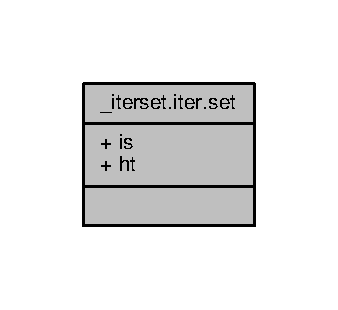
\includegraphics[width=162pt]{unionzsetopsrc_1_1__iterset_8iter_8set__coll__graph}
\end{center}
\end{figure}
\subsection*{Data Fields}
\begin{DoxyCompactItemize}
\item 
\mbox{\Hypertarget{unionzsetopsrc_1_1__iterset_8iter_8set_aa2a551a6458a8de22446cc76d639a9e9}\label{unionzsetopsrc_1_1__iterset_8iter_8set_aa2a551a6458a8de22446cc76d639a9e9}} 
\begin{tabbing}
xx\=xx\=xx\=xx\=xx\=xx\=xx\=xx\=xx\=\kill
struct \{\\
\mbox{\Hypertarget{structzsetopsrc_1_1_0D15_1_1__iterset_1_1_0D16_a74047218327de788518ec9960b3ec1a5}\label{structzsetopsrc_1_1_0D15_1_1__iterset_1_1_0D16_a74047218327de788518ec9960b3ec1a5}} 
\hyperlink{structintset}{intset} $\ast$ {\bfseries is}\\
\mbox{\Hypertarget{structzsetopsrc_1_1_0D15_1_1__iterset_1_1_0D16_adf0be69cd3479bce443c0c6fe913e405}\label{structzsetopsrc_1_1_0D15_1_1__iterset_1_1_0D16_adf0be69cd3479bce443c0c6fe913e405}} 
int {\bfseries ii}\\
\} {\bfseries is}\\

\end{tabbing}\item 
\mbox{\Hypertarget{unionzsetopsrc_1_1__iterset_8iter_8set_aeb5e48e74123cacc52761302ea4a7d22}\label{unionzsetopsrc_1_1__iterset_8iter_8set_aeb5e48e74123cacc52761302ea4a7d22}} 
\begin{tabbing}
xx\=xx\=xx\=xx\=xx\=xx\=xx\=xx\=xx\=\kill
struct \{\\
\mbox{\Hypertarget{structzsetopsrc_1_1_0D15_1_1__iterset_1_1_0D17_aa0767f4d2c012a7efea7e6a0a3354de9}\label{structzsetopsrc_1_1_0D15_1_1__iterset_1_1_0D17_aa0767f4d2c012a7efea7e6a0a3354de9}} 
\hyperlink{structdict}{dict} $\ast$ {\bfseries dict}\\
\mbox{\Hypertarget{structzsetopsrc_1_1_0D15_1_1__iterset_1_1_0D17_af661994566a00d1facee19bb451f0d11}\label{structzsetopsrc_1_1_0D15_1_1__iterset_1_1_0D17_af661994566a00d1facee19bb451f0d11}} 
\hyperlink{structdictIterator}{dictIterator} $\ast$ {\bfseries di}\\
\mbox{\Hypertarget{structzsetopsrc_1_1_0D15_1_1__iterset_1_1_0D17_ae6bfeec38e5d09bdcb6513e2dd08ce29}\label{structzsetopsrc_1_1_0D15_1_1__iterset_1_1_0D17_ae6bfeec38e5d09bdcb6513e2dd08ce29}} 
\hyperlink{structdictEntry}{dictEntry} $\ast$ {\bfseries de}\\
\} {\bfseries ht}\\

\end{tabbing}\end{DoxyCompactItemize}


\subsection{Detailed Description}


Definition at line \hyperlink{t__zset_8c_source_l01767}{1767} of file \hyperlink{t__zset_8c_source}{t\+\_\+zset.\+c}.



\subsection{Field Documentation}
\mbox{\Hypertarget{unionzsetopsrc_1_1__iterset_8iter_8set_aeb5e48e74123cacc52761302ea4a7d22}\label{unionzsetopsrc_1_1__iterset_8iter_8set_aeb5e48e74123cacc52761302ea4a7d22}} 
\index{zsetopsrc\+::\+\_\+iterset.\+iter.\+set@{zsetopsrc\+::\+\_\+iterset.\+iter.\+set}!ht@{ht}}
\index{ht@{ht}!zsetopsrc\+::\+\_\+iterset.\+iter.\+set@{zsetopsrc\+::\+\_\+iterset.\+iter.\+set}}
\subsubsection{\texorpdfstring{ht}{ht}}
{\footnotesize\ttfamily }

\mbox{\Hypertarget{unionzsetopsrc_1_1__iterset_8iter_8set_aa2a551a6458a8de22446cc76d639a9e9}\label{unionzsetopsrc_1_1__iterset_8iter_8set_aa2a551a6458a8de22446cc76d639a9e9}} 
\index{zsetopsrc\+::\+\_\+iterset.\+iter.\+set@{zsetopsrc\+::\+\_\+iterset.\+iter.\+set}!is@{is}}
\index{is@{is}!zsetopsrc\+::\+\_\+iterset.\+iter.\+set@{zsetopsrc\+::\+\_\+iterset.\+iter.\+set}}
\subsubsection{\texorpdfstring{is}{is}}
{\footnotesize\ttfamily }



The documentation for this union was generated from the following files\+:
\hypertarget{structzsetopsrc_1_1__iterset_8iter_8set_8ht}{}\section{\+\_\+iterset.\+iter.\+set.\+ht Struct Reference}
\label{structzsetopsrc_1_1__iterset_8iter_8set_8ht}\index{\+\_\+iterset.\+iter.\+set.\+ht@{\+\_\+iterset.\+iter.\+set.\+ht}}


Collaboration diagram for \+\_\+iterset.\+iter.\+set.\+ht\+:\nopagebreak
\begin{figure}[H]
\begin{center}
\leavevmode
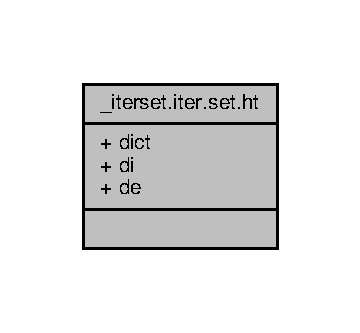
\includegraphics[width=173pt]{structzsetopsrc_1_1__iterset_8iter_8set_8ht__coll__graph}
\end{center}
\end{figure}
\subsection*{Data Fields}
\begin{DoxyCompactItemize}
\item 
\mbox{\Hypertarget{structzsetopsrc_1_1__iterset_8iter_8set_8ht_abb4c374392133719a324ab1ba2799cd6}\label{structzsetopsrc_1_1__iterset_8iter_8set_8ht_abb4c374392133719a324ab1ba2799cd6}} 
\hyperlink{structdict}{dict} $\ast$ {\bfseries dict}
\item 
\mbox{\Hypertarget{structzsetopsrc_1_1__iterset_8iter_8set_8ht_a690382ddccb8abc7367a136262e1978f}\label{structzsetopsrc_1_1__iterset_8iter_8set_8ht_a690382ddccb8abc7367a136262e1978f}} 
\hyperlink{structdictIterator}{dict\+Iterator} $\ast$ {\bfseries di}
\item 
\mbox{\Hypertarget{structzsetopsrc_1_1__iterset_8iter_8set_8ht_a5f02f0889301fd7be1ac972c11bf3e7d}\label{structzsetopsrc_1_1__iterset_8iter_8set_8ht_a5f02f0889301fd7be1ac972c11bf3e7d}} 
\hyperlink{structdictEntry}{dict\+Entry} $\ast$ {\bfseries de}
\end{DoxyCompactItemize}


\subsection{Detailed Description}


Definition at line \hyperlink{t__zset_8c_source_l01772}{1772} of file \hyperlink{t__zset_8c_source}{t\+\_\+zset.\+c}.



\subsection{Field Documentation}
\mbox{\Hypertarget{structzsetopsrc_1_1__iterset_8iter_8set_8ht_a5f02f0889301fd7be1ac972c11bf3e7d}\label{structzsetopsrc_1_1__iterset_8iter_8set_8ht_a5f02f0889301fd7be1ac972c11bf3e7d}} 
\index{zsetopsrc\+::\+\_\+iterset.\+iter.\+set.\+ht@{zsetopsrc\+::\+\_\+iterset.\+iter.\+set.\+ht}!de@{de}}
\index{de@{de}!zsetopsrc\+::\+\_\+iterset.\+iter.\+set.\+ht@{zsetopsrc\+::\+\_\+iterset.\+iter.\+set.\+ht}}
\subsubsection{\texorpdfstring{de}{de}}
{\footnotesize\ttfamily }

\mbox{\Hypertarget{structzsetopsrc_1_1__iterset_8iter_8set_8ht_a690382ddccb8abc7367a136262e1978f}\label{structzsetopsrc_1_1__iterset_8iter_8set_8ht_a690382ddccb8abc7367a136262e1978f}} 
\index{zsetopsrc\+::\+\_\+iterset.\+iter.\+set.\+ht@{zsetopsrc\+::\+\_\+iterset.\+iter.\+set.\+ht}!di@{di}}
\index{di@{di}!zsetopsrc\+::\+\_\+iterset.\+iter.\+set.\+ht@{zsetopsrc\+::\+\_\+iterset.\+iter.\+set.\+ht}}
\subsubsection{\texorpdfstring{di}{di}}
{\footnotesize\ttfamily }

\mbox{\Hypertarget{structzsetopsrc_1_1__iterset_8iter_8set_8ht_abb4c374392133719a324ab1ba2799cd6}\label{structzsetopsrc_1_1__iterset_8iter_8set_8ht_abb4c374392133719a324ab1ba2799cd6}} 
\index{zsetopsrc\+::\+\_\+iterset.\+iter.\+set.\+ht@{zsetopsrc\+::\+\_\+iterset.\+iter.\+set.\+ht}!dict@{dict}}
\index{dict@{dict}!zsetopsrc\+::\+\_\+iterset.\+iter.\+set.\+ht@{zsetopsrc\+::\+\_\+iterset.\+iter.\+set.\+ht}}
\subsubsection{\texorpdfstring{dict}{dict}}
{\footnotesize\ttfamily }



The documentation for this struct was generated from the following files\+:
\hypertarget{structzsetopsrc_1_1__iterset_8iter_8set_8is}{}\section{\+\_\+iterset.\+iter.\+set.\+is Struct Reference}
\label{structzsetopsrc_1_1__iterset_8iter_8set_8is}\index{\+\_\+iterset.\+iter.\+set.\+is@{\+\_\+iterset.\+iter.\+set.\+is}}


Collaboration diagram for \+\_\+iterset.\+iter.\+set.\+is\+:\nopagebreak
\begin{figure}[H]
\begin{center}
\leavevmode
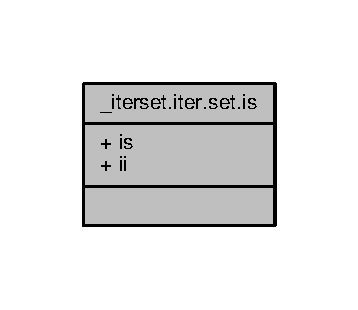
\includegraphics[width=172pt]{structzsetopsrc_1_1__iterset_8iter_8set_8is__coll__graph}
\end{center}
\end{figure}
\subsection*{Data Fields}
\begin{DoxyCompactItemize}
\item 
\mbox{\Hypertarget{structzsetopsrc_1_1__iterset_8iter_8set_8is_aa2a551a6458a8de22446cc76d639a9e9}\label{structzsetopsrc_1_1__iterset_8iter_8set_8is_aa2a551a6458a8de22446cc76d639a9e9}} 
\hyperlink{structintset}{intset} $\ast$ {\bfseries is}
\item 
\mbox{\Hypertarget{structzsetopsrc_1_1__iterset_8iter_8set_8is_a7e98b8a17c0aad30ba64d47b74e2a6c1}\label{structzsetopsrc_1_1__iterset_8iter_8set_8is_a7e98b8a17c0aad30ba64d47b74e2a6c1}} 
int {\bfseries ii}
\end{DoxyCompactItemize}


\subsection{Detailed Description}


Definition at line \hyperlink{t__zset_8c_source_l01768}{1768} of file \hyperlink{t__zset_8c_source}{t\+\_\+zset.\+c}.



\subsection{Field Documentation}
\mbox{\Hypertarget{structzsetopsrc_1_1__iterset_8iter_8set_8is_a7e98b8a17c0aad30ba64d47b74e2a6c1}\label{structzsetopsrc_1_1__iterset_8iter_8set_8is_a7e98b8a17c0aad30ba64d47b74e2a6c1}} 
\index{zsetopsrc\+::\+\_\+iterset.\+iter.\+set.\+is@{zsetopsrc\+::\+\_\+iterset.\+iter.\+set.\+is}!ii@{ii}}
\index{ii@{ii}!zsetopsrc\+::\+\_\+iterset.\+iter.\+set.\+is@{zsetopsrc\+::\+\_\+iterset.\+iter.\+set.\+is}}
\subsubsection{\texorpdfstring{ii}{ii}}
{\footnotesize\ttfamily }

\mbox{\Hypertarget{structzsetopsrc_1_1__iterset_8iter_8set_8is_aa2a551a6458a8de22446cc76d639a9e9}\label{structzsetopsrc_1_1__iterset_8iter_8set_8is_aa2a551a6458a8de22446cc76d639a9e9}} 
\index{zsetopsrc\+::\+\_\+iterset.\+iter.\+set.\+is@{zsetopsrc\+::\+\_\+iterset.\+iter.\+set.\+is}!is@{is}}
\index{is@{is}!zsetopsrc\+::\+\_\+iterset.\+iter.\+set.\+is@{zsetopsrc\+::\+\_\+iterset.\+iter.\+set.\+is}}
\subsubsection{\texorpdfstring{is}{is}}
{\footnotesize\ttfamily }



The documentation for this struct was generated from the following files\+:
\hypertarget{unionzsetopsrc_1_1__iterzset_8iter_8zset}{}\section{\+\_\+iterzset.\+iter.\+zset Union Reference}
\label{unionzsetopsrc_1_1__iterzset_8iter_8zset}\index{\+\_\+iterzset.\+iter.\+zset@{\+\_\+iterzset.\+iter.\+zset}}


Collaboration diagram for \+\_\+iterzset.\+iter.\+zset\+:\nopagebreak
\begin{figure}[H]
\begin{center}
\leavevmode
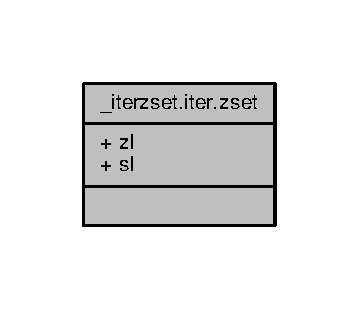
\includegraphics[width=172pt]{unionzsetopsrc_1_1__iterzset_8iter_8zset__coll__graph}
\end{center}
\end{figure}
\subsection*{Data Fields}
\begin{DoxyCompactItemize}
\item 
\mbox{\Hypertarget{unionzsetopsrc_1_1__iterzset_8iter_8zset_ac28cbd398a61e9022fd6a6835a57dc50}\label{unionzsetopsrc_1_1__iterzset_8iter_8zset_ac28cbd398a61e9022fd6a6835a57dc50}} 
\begin{tabbing}
xx\=xx\=xx\=xx\=xx\=xx\=xx\=xx\=xx\=\kill
struct \{\\
\mbox{\Hypertarget{structzsetopsrc_1_1_0D15_1_1__iterzset_1_1_0D18_abba72f04a4d287a7d2caa8337a57bc1b}\label{structzsetopsrc_1_1_0D15_1_1__iterzset_1_1_0D18_abba72f04a4d287a7d2caa8337a57bc1b}} 
unsigned char $\ast$ {\bfseries zl}\\
\mbox{\Hypertarget{structzsetopsrc_1_1_0D15_1_1__iterzset_1_1_0D18_ad4d9472b36dd51beb817be8803c0b9aa}\label{structzsetopsrc_1_1_0D15_1_1__iterzset_1_1_0D18_ad4d9472b36dd51beb817be8803c0b9aa}} 
unsigned char $\ast$ {\bfseries eptr}\\
\mbox{\Hypertarget{structzsetopsrc_1_1_0D15_1_1__iterzset_1_1_0D18_af4f11a2890160f3a07fa3d508c60ceda}\label{structzsetopsrc_1_1_0D15_1_1__iterzset_1_1_0D18_af4f11a2890160f3a07fa3d508c60ceda}} 
unsigned char $\ast$ {\bfseries sptr}\\
\} {\bfseries zl}\\

\end{tabbing}\item 
\mbox{\Hypertarget{unionzsetopsrc_1_1__iterzset_8iter_8zset_a54a2bf8c09ace67d3513aaa1aa7aa0f3}\label{unionzsetopsrc_1_1__iterzset_8iter_8zset_a54a2bf8c09ace67d3513aaa1aa7aa0f3}} 
\begin{tabbing}
xx\=xx\=xx\=xx\=xx\=xx\=xx\=xx\=xx\=\kill
struct \{\\
\mbox{\Hypertarget{structzsetopsrc_1_1_0D15_1_1__iterzset_1_1_0D19_a9aeae9b092dd392b29d133a9bb89f106}\label{structzsetopsrc_1_1_0D15_1_1__iterzset_1_1_0D19_a9aeae9b092dd392b29d133a9bb89f106}} 
\hyperlink{structzset}{zset} $\ast$ {\bfseries zs}\\
\mbox{\Hypertarget{structzsetopsrc_1_1_0D15_1_1__iterzset_1_1_0D19_a8fddead5a211a1f361c5411ec030e487}\label{structzsetopsrc_1_1_0D15_1_1__iterzset_1_1_0D19_a8fddead5a211a1f361c5411ec030e487}} 
\hyperlink{structzskiplistNode}{zskiplistNode} $\ast$ {\bfseries node}\\
\} {\bfseries sl}\\

\end{tabbing}\end{DoxyCompactItemize}


\subsection{Detailed Description}


Definition at line \hyperlink{t__zset_8c_source_l01780}{1780} of file \hyperlink{t__zset_8c_source}{t\+\_\+zset.\+c}.



\subsection{Field Documentation}
\mbox{\Hypertarget{unionzsetopsrc_1_1__iterzset_8iter_8zset_a54a2bf8c09ace67d3513aaa1aa7aa0f3}\label{unionzsetopsrc_1_1__iterzset_8iter_8zset_a54a2bf8c09ace67d3513aaa1aa7aa0f3}} 
\index{zsetopsrc\+::\+\_\+iterzset.\+iter.\+zset@{zsetopsrc\+::\+\_\+iterzset.\+iter.\+zset}!sl@{sl}}
\index{sl@{sl}!zsetopsrc\+::\+\_\+iterzset.\+iter.\+zset@{zsetopsrc\+::\+\_\+iterzset.\+iter.\+zset}}
\subsubsection{\texorpdfstring{sl}{sl}}
{\footnotesize\ttfamily }

\mbox{\Hypertarget{unionzsetopsrc_1_1__iterzset_8iter_8zset_ac28cbd398a61e9022fd6a6835a57dc50}\label{unionzsetopsrc_1_1__iterzset_8iter_8zset_ac28cbd398a61e9022fd6a6835a57dc50}} 
\index{zsetopsrc\+::\+\_\+iterzset.\+iter.\+zset@{zsetopsrc\+::\+\_\+iterzset.\+iter.\+zset}!zl@{zl}}
\index{zl@{zl}!zsetopsrc\+::\+\_\+iterzset.\+iter.\+zset@{zsetopsrc\+::\+\_\+iterzset.\+iter.\+zset}}
\subsubsection{\texorpdfstring{zl}{zl}}
{\footnotesize\ttfamily }



The documentation for this union was generated from the following files\+:
\hypertarget{structzsetopsrc_1_1__iterzset_8iter_8zset_8sl}{}\section{\+\_\+iterzset.\+iter.\+zset.\+sl Struct Reference}
\label{structzsetopsrc_1_1__iterzset_8iter_8zset_8sl}\index{\+\_\+iterzset.\+iter.\+zset.\+sl@{\+\_\+iterzset.\+iter.\+zset.\+sl}}


Collaboration diagram for \+\_\+iterzset.\+iter.\+zset.\+sl\+:\nopagebreak
\begin{figure}[H]
\begin{center}
\leavevmode
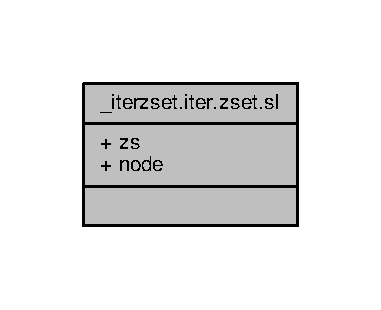
\includegraphics[width=183pt]{structzsetopsrc_1_1__iterzset_8iter_8zset_8sl__coll__graph}
\end{center}
\end{figure}
\subsection*{Data Fields}
\begin{DoxyCompactItemize}
\item 
\mbox{\Hypertarget{structzsetopsrc_1_1__iterzset_8iter_8zset_8sl_af6706d5db3ad094cfabd8fb5326f1eec}\label{structzsetopsrc_1_1__iterzset_8iter_8zset_8sl_af6706d5db3ad094cfabd8fb5326f1eec}} 
\hyperlink{structzset}{zset} $\ast$ {\bfseries zs}
\item 
\mbox{\Hypertarget{structzsetopsrc_1_1__iterzset_8iter_8zset_8sl_a36c4536996ca5615dcf9911f068786dc}\label{structzsetopsrc_1_1__iterzset_8iter_8zset_8sl_a36c4536996ca5615dcf9911f068786dc}} 
\hyperlink{structzskiplistNode}{zskiplist\+Node} $\ast$ {\bfseries node}
\end{DoxyCompactItemize}


\subsection{Detailed Description}


Definition at line \hyperlink{t__zset_8c_source_l01785}{1785} of file \hyperlink{t__zset_8c_source}{t\+\_\+zset.\+c}.



\subsection{Field Documentation}
\mbox{\Hypertarget{structzsetopsrc_1_1__iterzset_8iter_8zset_8sl_a36c4536996ca5615dcf9911f068786dc}\label{structzsetopsrc_1_1__iterzset_8iter_8zset_8sl_a36c4536996ca5615dcf9911f068786dc}} 
\index{zsetopsrc\+::\+\_\+iterzset.\+iter.\+zset.\+sl@{zsetopsrc\+::\+\_\+iterzset.\+iter.\+zset.\+sl}!node@{node}}
\index{node@{node}!zsetopsrc\+::\+\_\+iterzset.\+iter.\+zset.\+sl@{zsetopsrc\+::\+\_\+iterzset.\+iter.\+zset.\+sl}}
\subsubsection{\texorpdfstring{node}{node}}
{\footnotesize\ttfamily }

\mbox{\Hypertarget{structzsetopsrc_1_1__iterzset_8iter_8zset_8sl_af6706d5db3ad094cfabd8fb5326f1eec}\label{structzsetopsrc_1_1__iterzset_8iter_8zset_8sl_af6706d5db3ad094cfabd8fb5326f1eec}} 
\index{zsetopsrc\+::\+\_\+iterzset.\+iter.\+zset.\+sl@{zsetopsrc\+::\+\_\+iterzset.\+iter.\+zset.\+sl}!zs@{zs}}
\index{zs@{zs}!zsetopsrc\+::\+\_\+iterzset.\+iter.\+zset.\+sl@{zsetopsrc\+::\+\_\+iterzset.\+iter.\+zset.\+sl}}
\subsubsection{\texorpdfstring{zs}{zs}}
{\footnotesize\ttfamily }



The documentation for this struct was generated from the following files\+:
\hypertarget{structzsetopsrc_1_1__iterzset_8iter_8zset_8zl}{}\section{\+\_\+iterzset.\+iter.\+zset.\+zl Struct Reference}
\label{structzsetopsrc_1_1__iterzset_8iter_8zset_8zl}\index{\+\_\+iterzset.\+iter.\+zset.\+zl@{\+\_\+iterzset.\+iter.\+zset.\+zl}}


Collaboration diagram for \+\_\+iterzset.\+iter.\+zset.\+zl\+:\nopagebreak
\begin{figure}[H]
\begin{center}
\leavevmode
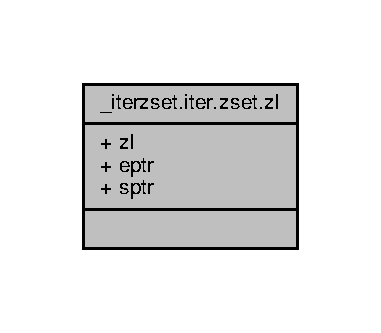
\includegraphics[width=183pt]{structzsetopsrc_1_1__iterzset_8iter_8zset_8zl__coll__graph}
\end{center}
\end{figure}
\subsection*{Data Fields}
\begin{DoxyCompactItemize}
\item 
\mbox{\Hypertarget{structzsetopsrc_1_1__iterzset_8iter_8zset_8zl_ac28cbd398a61e9022fd6a6835a57dc50}\label{structzsetopsrc_1_1__iterzset_8iter_8zset_8zl_ac28cbd398a61e9022fd6a6835a57dc50}} 
unsigned char $\ast$ {\bfseries zl}
\item 
\mbox{\Hypertarget{structzsetopsrc_1_1__iterzset_8iter_8zset_8zl_afac7b97084c84e109b45fe4ac53a63c0}\label{structzsetopsrc_1_1__iterzset_8iter_8zset_8zl_afac7b97084c84e109b45fe4ac53a63c0}} 
unsigned char $\ast$ {\bfseries eptr}
\item 
\mbox{\Hypertarget{structzsetopsrc_1_1__iterzset_8iter_8zset_8zl_aa6769fcc80318f1732ac9dbf2bc2511d}\label{structzsetopsrc_1_1__iterzset_8iter_8zset_8zl_aa6769fcc80318f1732ac9dbf2bc2511d}} 
unsigned char $\ast$ {\bfseries sptr}
\end{DoxyCompactItemize}


\subsection{Detailed Description}


Definition at line \hyperlink{t__zset_8c_source_l01781}{1781} of file \hyperlink{t__zset_8c_source}{t\+\_\+zset.\+c}.



\subsection{Field Documentation}
\mbox{\Hypertarget{structzsetopsrc_1_1__iterzset_8iter_8zset_8zl_afac7b97084c84e109b45fe4ac53a63c0}\label{structzsetopsrc_1_1__iterzset_8iter_8zset_8zl_afac7b97084c84e109b45fe4ac53a63c0}} 
\index{zsetopsrc\+::\+\_\+iterzset.\+iter.\+zset.\+zl@{zsetopsrc\+::\+\_\+iterzset.\+iter.\+zset.\+zl}!eptr@{eptr}}
\index{eptr@{eptr}!zsetopsrc\+::\+\_\+iterzset.\+iter.\+zset.\+zl@{zsetopsrc\+::\+\_\+iterzset.\+iter.\+zset.\+zl}}
\subsubsection{\texorpdfstring{eptr}{eptr}}
{\footnotesize\ttfamily }

\mbox{\Hypertarget{structzsetopsrc_1_1__iterzset_8iter_8zset_8zl_aa6769fcc80318f1732ac9dbf2bc2511d}\label{structzsetopsrc_1_1__iterzset_8iter_8zset_8zl_aa6769fcc80318f1732ac9dbf2bc2511d}} 
\index{zsetopsrc\+::\+\_\+iterzset.\+iter.\+zset.\+zl@{zsetopsrc\+::\+\_\+iterzset.\+iter.\+zset.\+zl}!sptr@{sptr}}
\index{sptr@{sptr}!zsetopsrc\+::\+\_\+iterzset.\+iter.\+zset.\+zl@{zsetopsrc\+::\+\_\+iterzset.\+iter.\+zset.\+zl}}
\subsubsection{\texorpdfstring{sptr}{sptr}}
{\footnotesize\ttfamily }

\mbox{\Hypertarget{structzsetopsrc_1_1__iterzset_8iter_8zset_8zl_ac28cbd398a61e9022fd6a6835a57dc50}\label{structzsetopsrc_1_1__iterzset_8iter_8zset_8zl_ac28cbd398a61e9022fd6a6835a57dc50}} 
\index{zsetopsrc\+::\+\_\+iterzset.\+iter.\+zset.\+zl@{zsetopsrc\+::\+\_\+iterzset.\+iter.\+zset.\+zl}!zl@{zl}}
\index{zl@{zl}!zsetopsrc\+::\+\_\+iterzset.\+iter.\+zset.\+zl@{zsetopsrc\+::\+\_\+iterzset.\+iter.\+zset.\+zl}}
\subsubsection{\texorpdfstring{zl}{zl}}
{\footnotesize\ttfamily }



The documentation for this struct was generated from the following files\+:
\hypertarget{struct__redisSortObject}{}\section{\+\_\+redis\+Sort\+Object Struct Reference}
\label{struct__redisSortObject}\index{\+\_\+redis\+Sort\+Object@{\+\_\+redis\+Sort\+Object}}


Collaboration diagram for \+\_\+redis\+Sort\+Object\+:\nopagebreak
\begin{figure}[H]
\begin{center}
\leavevmode
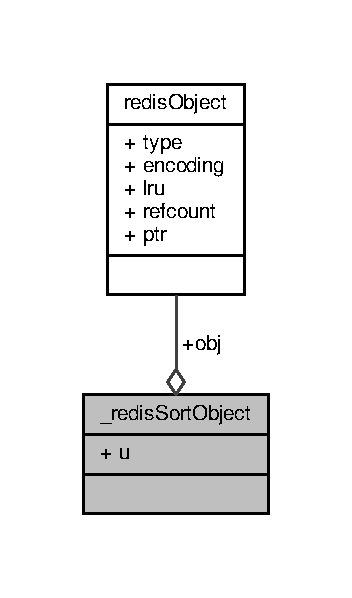
\includegraphics[width=169pt]{struct__redisSortObject__coll__graph}
\end{center}
\end{figure}
\subsection*{Data Fields}
\begin{DoxyCompactItemize}
\item 
\mbox{\Hypertarget{struct__redisSortObject_a4537823adb41ac7cc390fc3e6ef20969}\label{struct__redisSortObject_a4537823adb41ac7cc390fc3e6ef20969}} 
\hyperlink{structredisObject}{robj} $\ast$ {\bfseries obj}
\item 
\mbox{\Hypertarget{struct__redisSortObject_ac8b897d5e08a1b3a0257d4ebec6f3146}\label{struct__redisSortObject_ac8b897d5e08a1b3a0257d4ebec6f3146}} 
\begin{tabbing}
xx\=xx\=xx\=xx\=xx\=xx\=xx\=xx\=xx\=\kill
union \{\\
\mbox{\Hypertarget{struct__redisSortObject_a8b20a0ac67a22f100cb44039985048e3}\label{struct__redisSortObject_a8b20a0ac67a22f100cb44039985048e3}} 
double {\bfseries score}\\
\mbox{\Hypertarget{struct__redisSortObject_ae0dfac5206eb3a811ca122f2acd5ab0d}\label{struct__redisSortObject_ae0dfac5206eb3a811ca122f2acd5ab0d}} 
\hyperlink{structredisObject}{robj} $\ast$ {\bfseries cmpobj}\\
\} {\bfseries u}\\

\end{tabbing}\end{DoxyCompactItemize}


\subsection{Detailed Description}


Definition at line \hyperlink{server_8h_source_l01245}{1245} of file \hyperlink{server_8h_source}{server.\+h}.



\subsection{Field Documentation}
\mbox{\Hypertarget{struct__redisSortObject_a4537823adb41ac7cc390fc3e6ef20969}\label{struct__redisSortObject_a4537823adb41ac7cc390fc3e6ef20969}} 
\index{\+\_\+redis\+Sort\+Object@{\+\_\+redis\+Sort\+Object}!obj@{obj}}
\index{obj@{obj}!\+\_\+redis\+Sort\+Object@{\+\_\+redis\+Sort\+Object}}
\subsubsection{\texorpdfstring{obj}{obj}}
{\footnotesize\ttfamily \hyperlink{structredisObject}{robj}$\ast$ \+\_\+redis\+Sort\+Object\+::obj}



Definition at line \hyperlink{server_8h_source_l01246}{1246} of file \hyperlink{server_8h_source}{server.\+h}.

\mbox{\Hypertarget{struct__redisSortObject_ac8b897d5e08a1b3a0257d4ebec6f3146}\label{struct__redisSortObject_ac8b897d5e08a1b3a0257d4ebec6f3146}} 
\index{\+\_\+redis\+Sort\+Object@{\+\_\+redis\+Sort\+Object}!u@{u}}
\index{u@{u}!\+\_\+redis\+Sort\+Object@{\+\_\+redis\+Sort\+Object}}
\subsubsection{\texorpdfstring{u}{u}}
{\footnotesize\ttfamily union \{ ... \}   \+\_\+redis\+Sort\+Object\+::u}



The documentation for this struct was generated from the following file\+:\begin{DoxyCompactItemize}
\item 
src/server.\+h\end{DoxyCompactItemize}

\hypertarget{union__redisSortObject_8u}{}\section{\+\_\+redis\+Sort\+Object.\+u Union Reference}
\label{union__redisSortObject_8u}\index{\+\_\+redis\+Sort\+Object.\+u@{\+\_\+redis\+Sort\+Object.\+u}}


Collaboration diagram for \+\_\+redis\+Sort\+Object.\+u\+:\nopagebreak
\begin{figure}[H]
\begin{center}
\leavevmode
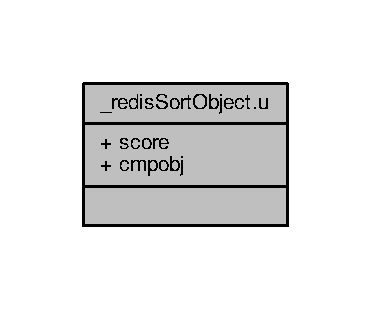
\includegraphics[width=178pt]{union__redisSortObject_8u__coll__graph}
\end{center}
\end{figure}
\subsection*{Data Fields}
\begin{DoxyCompactItemize}
\item 
\mbox{\Hypertarget{union__redisSortObject_8u_aca1cd3c3055991bf20499ee86739f7e2}\label{union__redisSortObject_8u_aca1cd3c3055991bf20499ee86739f7e2}} 
double {\bfseries score}
\item 
\mbox{\Hypertarget{union__redisSortObject_8u_aa5848be22772156621af135260c2210f}\label{union__redisSortObject_8u_aa5848be22772156621af135260c2210f}} 
\hyperlink{structredisObject}{robj} $\ast$ {\bfseries cmpobj}
\end{DoxyCompactItemize}


\subsection{Detailed Description}


Definition at line \hyperlink{server_8h_source_l01247}{1247} of file \hyperlink{server_8h_source}{server.\+h}.



\subsection{Field Documentation}
\mbox{\Hypertarget{union__redisSortObject_8u_aa5848be22772156621af135260c2210f}\label{union__redisSortObject_8u_aa5848be22772156621af135260c2210f}} 
\index{\+\_\+redis\+Sort\+Object.\+u@{\+\_\+redis\+Sort\+Object.\+u}!cmpobj@{cmpobj}}
\index{cmpobj@{cmpobj}!\+\_\+redis\+Sort\+Object.\+u@{\+\_\+redis\+Sort\+Object.\+u}}
\subsubsection{\texorpdfstring{cmpobj}{cmpobj}}
{\footnotesize\ttfamily }

\mbox{\Hypertarget{union__redisSortObject_8u_aca1cd3c3055991bf20499ee86739f7e2}\label{union__redisSortObject_8u_aca1cd3c3055991bf20499ee86739f7e2}} 
\index{\+\_\+redis\+Sort\+Object.\+u@{\+\_\+redis\+Sort\+Object.\+u}!score@{score}}
\index{score@{score}!\+\_\+redis\+Sort\+Object.\+u@{\+\_\+redis\+Sort\+Object.\+u}}
\subsubsection{\texorpdfstring{score}{score}}
{\footnotesize\ttfamily }



The documentation for this union was generated from the following files\+:
\hypertarget{struct__redisSortOperation}{}\section{\+\_\+redis\+Sort\+Operation Struct Reference}
\label{struct__redisSortOperation}\index{\+\_\+redis\+Sort\+Operation@{\+\_\+redis\+Sort\+Operation}}


Collaboration diagram for \+\_\+redis\+Sort\+Operation\+:\nopagebreak
\begin{figure}[H]
\begin{center}
\leavevmode
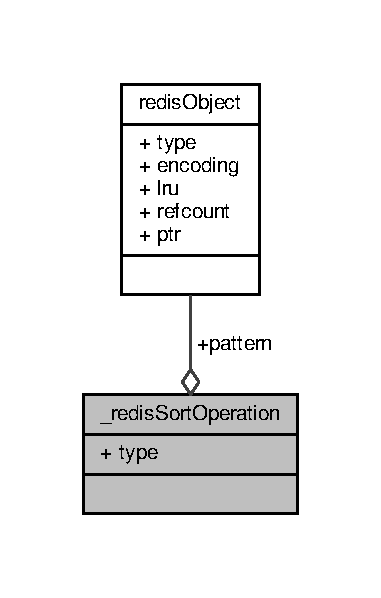
\includegraphics[width=183pt]{struct__redisSortOperation__coll__graph}
\end{center}
\end{figure}
\subsection*{Data Fields}
\begin{DoxyCompactItemize}
\item 
\mbox{\Hypertarget{struct__redisSortOperation_aa15685700428f4fe6cb63518eb8c5adc}\label{struct__redisSortOperation_aa15685700428f4fe6cb63518eb8c5adc}} 
int {\bfseries type}
\item 
\mbox{\Hypertarget{struct__redisSortOperation_adf9bf02d385c5a695c4a2b93bd6a4b0f}\label{struct__redisSortOperation_adf9bf02d385c5a695c4a2b93bd6a4b0f}} 
\hyperlink{structredisObject}{robj} $\ast$ {\bfseries pattern}
\end{DoxyCompactItemize}


\subsection{Detailed Description}


Definition at line \hyperlink{server_8h_source_l01253}{1253} of file \hyperlink{server_8h_source}{server.\+h}.



\subsection{Field Documentation}
\mbox{\Hypertarget{struct__redisSortOperation_adf9bf02d385c5a695c4a2b93bd6a4b0f}\label{struct__redisSortOperation_adf9bf02d385c5a695c4a2b93bd6a4b0f}} 
\index{\+\_\+redis\+Sort\+Operation@{\+\_\+redis\+Sort\+Operation}!pattern@{pattern}}
\index{pattern@{pattern}!\+\_\+redis\+Sort\+Operation@{\+\_\+redis\+Sort\+Operation}}
\subsubsection{\texorpdfstring{pattern}{pattern}}
{\footnotesize\ttfamily \hyperlink{structredisObject}{robj}$\ast$ \+\_\+redis\+Sort\+Operation\+::pattern}



Definition at line \hyperlink{server_8h_source_l01255}{1255} of file \hyperlink{server_8h_source}{server.\+h}.

\mbox{\Hypertarget{struct__redisSortOperation_aa15685700428f4fe6cb63518eb8c5adc}\label{struct__redisSortOperation_aa15685700428f4fe6cb63518eb8c5adc}} 
\index{\+\_\+redis\+Sort\+Operation@{\+\_\+redis\+Sort\+Operation}!type@{type}}
\index{type@{type}!\+\_\+redis\+Sort\+Operation@{\+\_\+redis\+Sort\+Operation}}
\subsubsection{\texorpdfstring{type}{type}}
{\footnotesize\ttfamily int \+\_\+redis\+Sort\+Operation\+::type}



Definition at line \hyperlink{server_8h_source_l01254}{1254} of file \hyperlink{server_8h_source}{server.\+h}.



The documentation for this struct was generated from the following file\+:\begin{DoxyCompactItemize}
\item 
src/server.\+h\end{DoxyCompactItemize}

\hypertarget{struct__rio}{}\section{\+\_\+rio Struct Reference}
\label{struct__rio}\index{\+\_\+rio@{\+\_\+rio}}


Collaboration diagram for \+\_\+rio\+:\nopagebreak
\begin{figure}[H]
\begin{center}
\leavevmode
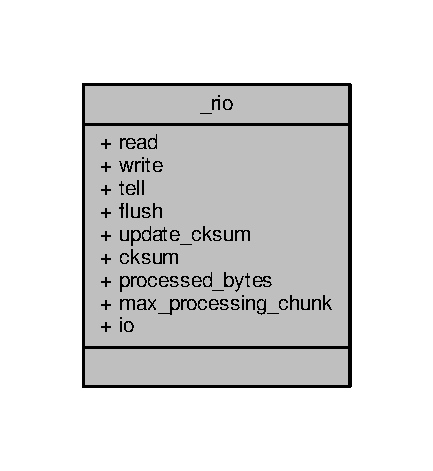
\includegraphics[width=208pt]{struct__rio__coll__graph}
\end{center}
\end{figure}
\subsection*{Data Fields}
\begin{DoxyCompactItemize}
\item 
\mbox{\Hypertarget{struct__rio_a8ebabb369aa4d0d56b6ffd2458d88576}\label{struct__rio_a8ebabb369aa4d0d56b6ffd2458d88576}} 
size\+\_\+t($\ast$ {\bfseries read} )(struct \hyperlink{struct__rio}{\+\_\+rio} $\ast$, void $\ast$buf, size\+\_\+t len)
\item 
\mbox{\Hypertarget{struct__rio_a8a7effb62e6010e71c1a87e9de88700d}\label{struct__rio_a8a7effb62e6010e71c1a87e9de88700d}} 
size\+\_\+t($\ast$ {\bfseries write} )(struct \hyperlink{struct__rio}{\+\_\+rio} $\ast$, const void $\ast$buf, size\+\_\+t len)
\item 
\mbox{\Hypertarget{struct__rio_a66ebd520b048b45e5603fe43f1b0abf9}\label{struct__rio_a66ebd520b048b45e5603fe43f1b0abf9}} 
off\+\_\+t($\ast$ {\bfseries tell} )(struct \hyperlink{struct__rio}{\+\_\+rio} $\ast$)
\item 
\mbox{\Hypertarget{struct__rio_a0efdc42cde18a29f94c7a848cab51c19}\label{struct__rio_a0efdc42cde18a29f94c7a848cab51c19}} 
int($\ast$ {\bfseries flush} )(struct \hyperlink{struct__rio}{\+\_\+rio} $\ast$)
\item 
\mbox{\Hypertarget{struct__rio_a26412d997c7a5e3df0e5d6fd3e604d52}\label{struct__rio_a26412d997c7a5e3df0e5d6fd3e604d52}} 
void($\ast$ {\bfseries update\+\_\+cksum} )(struct \hyperlink{struct__rio}{\+\_\+rio} $\ast$, const void $\ast$buf, size\+\_\+t len)
\item 
\mbox{\Hypertarget{struct__rio_af4d2fe2a30ae204624255e0f13d0cff8}\label{struct__rio_af4d2fe2a30ae204624255e0f13d0cff8}} 
uint64\+\_\+t {\bfseries cksum}
\item 
\mbox{\Hypertarget{struct__rio_a75ceca68d98b7db8ae88bc8d08f63909}\label{struct__rio_a75ceca68d98b7db8ae88bc8d08f63909}} 
size\+\_\+t {\bfseries processed\+\_\+bytes}
\item 
\mbox{\Hypertarget{struct__rio_a52f631ed1a65b561d661a91ee54fc882}\label{struct__rio_a52f631ed1a65b561d661a91ee54fc882}} 
size\+\_\+t {\bfseries max\+\_\+processing\+\_\+chunk}
\item 
\mbox{\Hypertarget{struct__rio_a47d4551b43c0212e749c9a2e7fe27f8c}\label{struct__rio_a47d4551b43c0212e749c9a2e7fe27f8c}} 
\begin{tabbing}
xx\=xx\=xx\=xx\=xx\=xx\=xx\=xx\=xx\=\kill
union \{\\
\mbox{\Hypertarget{struct__rio_aab2132e75d76d5a27996a3244325c017}\label{struct__rio_aab2132e75d76d5a27996a3244325c017}} 
\>struct \{\\
\mbox{\Hypertarget{struct__rio_1_1_0D4_1_1_0D5_a175860cfc91edbbf64ce42d8ce695d1b}\label{struct__rio_1_1_0D4_1_1_0D5_a175860cfc91edbbf64ce42d8ce695d1b}} 
sds {\bfseries ptr}\\
\mbox{\Hypertarget{struct__rio_1_1_0D4_1_1_0D5_a0c42b215f77fc14b6421fa6fdb42670c}\label{struct__rio_1_1_0D4_1_1_0D5_a0c42b215f77fc14b6421fa6fdb42670c}} 
off\_t {\bfseries pos}\\
\>\} {\bfseries buffer}\\
\mbox{\Hypertarget{struct__rio_ac5e372021f58f9b26bff3218d7e67553}\label{struct__rio_ac5e372021f58f9b26bff3218d7e67553}} 
\>struct \{\\
\mbox{\Hypertarget{struct__rio_1_1_0D4_1_1_0D6_af35cfd36bb629017491ca4c84ca95edb}\label{struct__rio_1_1_0D4_1_1_0D6_af35cfd36bb629017491ca4c84ca95edb}} 
FILE $\ast$ {\bfseries fp}\\
\mbox{\Hypertarget{struct__rio_1_1_0D4_1_1_0D6_a034dd277bfca618dd4905121a7945f9c}\label{struct__rio_1_1_0D4_1_1_0D6_a034dd277bfca618dd4905121a7945f9c}} 
off\_t {\bfseries buffered}\\
\mbox{\Hypertarget{struct__rio_1_1_0D4_1_1_0D6_ae678183a05d1aab21ccb7088d4e2c368}\label{struct__rio_1_1_0D4_1_1_0D6_ae678183a05d1aab21ccb7088d4e2c368}} 
off\_t {\bfseries autosync}\\
\>\} {\bfseries file}\\
\mbox{\Hypertarget{struct__rio_ad6f4c3dc077f482b6f6fe5f15153fdbf}\label{struct__rio_ad6f4c3dc077f482b6f6fe5f15153fdbf}} 
\>struct \{\\
\mbox{\Hypertarget{struct__rio_1_1_0D4_1_1_0D7_a7805e59e6aa34bf51914235caa1be6c4}\label{struct__rio_1_1_0D4_1_1_0D7_a7805e59e6aa34bf51914235caa1be6c4}} 
int $\ast$ {\bfseries fds}\\
\mbox{\Hypertarget{struct__rio_1_1_0D4_1_1_0D7_a22d57b0b9a9474fcbc93950b00e06395}\label{struct__rio_1_1_0D4_1_1_0D7_a22d57b0b9a9474fcbc93950b00e06395}} 
int $\ast$ {\bfseries state}\\
\mbox{\Hypertarget{struct__rio_1_1_0D4_1_1_0D7_a560eddd13fc5425161fca489bc13f165}\label{struct__rio_1_1_0D4_1_1_0D7_a560eddd13fc5425161fca489bc13f165}} 
int {\bfseries numfds}\\
\mbox{\Hypertarget{struct__rio_1_1_0D4_1_1_0D7_aa1ca4b916242c44445ca68f647fc0878}\label{struct__rio_1_1_0D4_1_1_0D7_aa1ca4b916242c44445ca68f647fc0878}} 
off\_t {\bfseries pos}\\
\mbox{\Hypertarget{struct__rio_1_1_0D4_1_1_0D7_ad5582e2496733a9bcb35e6e9306be331}\label{struct__rio_1_1_0D4_1_1_0D7_ad5582e2496733a9bcb35e6e9306be331}} 
sds {\bfseries buf}\\
\>\} {\bfseries fdset}\\
\} {\bfseries io}\\

\end{tabbing}\end{DoxyCompactItemize}


\subsection{Detailed Description}


Definition at line \hyperlink{rio_8h_source_l00039}{39} of file \hyperlink{rio_8h_source}{rio.\+h}.



The documentation for this struct was generated from the following file\+:\begin{DoxyCompactItemize}
\item 
src/rio.\+h\end{DoxyCompactItemize}

\hypertarget{union__rio_8io}{}\section{\+\_\+rio.\+io Union Reference}
\label{union__rio_8io}\index{\+\_\+rio.\+io@{\+\_\+rio.\+io}}


Collaboration diagram for \+\_\+rio.\+io\+:\nopagebreak
\begin{figure}[H]
\begin{center}
\leavevmode
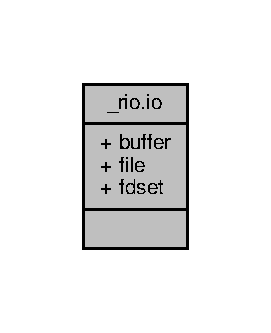
\includegraphics[width=130pt]{union__rio_8io__coll__graph}
\end{center}
\end{figure}
\subsection*{Data Fields}
\begin{DoxyCompactItemize}
\item 
\mbox{\Hypertarget{union__rio_8io_a7f2db423a49b305459147332fb01cf87}\label{union__rio_8io_a7f2db423a49b305459147332fb01cf87}} 
\begin{tabbing}
xx\=xx\=xx\=xx\=xx\=xx\=xx\=xx\=xx\=\kill
struct \{\\
\mbox{\Hypertarget{struct__rio_1_1_0D4_1_1_0D5_a175860cfc91edbbf64ce42d8ce695d1b}\label{struct__rio_1_1_0D4_1_1_0D5_a175860cfc91edbbf64ce42d8ce695d1b}} 
sds {\bfseries ptr}\\
\mbox{\Hypertarget{struct__rio_1_1_0D4_1_1_0D5_a0c42b215f77fc14b6421fa6fdb42670c}\label{struct__rio_1_1_0D4_1_1_0D5_a0c42b215f77fc14b6421fa6fdb42670c}} 
off\_t {\bfseries pos}\\
\} {\bfseries buffer}\\

\end{tabbing}\item 
\mbox{\Hypertarget{union__rio_8io_a8c7dd922ad47494fc02c388e12c00eac}\label{union__rio_8io_a8c7dd922ad47494fc02c388e12c00eac}} 
\begin{tabbing}
xx\=xx\=xx\=xx\=xx\=xx\=xx\=xx\=xx\=\kill
struct \{\\
\mbox{\Hypertarget{struct__rio_1_1_0D4_1_1_0D6_af35cfd36bb629017491ca4c84ca95edb}\label{struct__rio_1_1_0D4_1_1_0D6_af35cfd36bb629017491ca4c84ca95edb}} 
FILE $\ast$ {\bfseries fp}\\
\mbox{\Hypertarget{struct__rio_1_1_0D4_1_1_0D6_a034dd277bfca618dd4905121a7945f9c}\label{struct__rio_1_1_0D4_1_1_0D6_a034dd277bfca618dd4905121a7945f9c}} 
off\_t {\bfseries buffered}\\
\mbox{\Hypertarget{struct__rio_1_1_0D4_1_1_0D6_ae678183a05d1aab21ccb7088d4e2c368}\label{struct__rio_1_1_0D4_1_1_0D6_ae678183a05d1aab21ccb7088d4e2c368}} 
off\_t {\bfseries autosync}\\
\} {\bfseries file}\\

\end{tabbing}\item 
\mbox{\Hypertarget{union__rio_8io_a02576d32deb49384ad8ebc30550d8c29}\label{union__rio_8io_a02576d32deb49384ad8ebc30550d8c29}} 
\begin{tabbing}
xx\=xx\=xx\=xx\=xx\=xx\=xx\=xx\=xx\=\kill
struct \{\\
\mbox{\Hypertarget{struct__rio_1_1_0D4_1_1_0D7_a7805e59e6aa34bf51914235caa1be6c4}\label{struct__rio_1_1_0D4_1_1_0D7_a7805e59e6aa34bf51914235caa1be6c4}} 
int $\ast$ {\bfseries fds}\\
\mbox{\Hypertarget{struct__rio_1_1_0D4_1_1_0D7_a22d57b0b9a9474fcbc93950b00e06395}\label{struct__rio_1_1_0D4_1_1_0D7_a22d57b0b9a9474fcbc93950b00e06395}} 
int $\ast$ {\bfseries state}\\
\mbox{\Hypertarget{struct__rio_1_1_0D4_1_1_0D7_a560eddd13fc5425161fca489bc13f165}\label{struct__rio_1_1_0D4_1_1_0D7_a560eddd13fc5425161fca489bc13f165}} 
int {\bfseries numfds}\\
\mbox{\Hypertarget{struct__rio_1_1_0D4_1_1_0D7_aa1ca4b916242c44445ca68f647fc0878}\label{struct__rio_1_1_0D4_1_1_0D7_aa1ca4b916242c44445ca68f647fc0878}} 
off\_t {\bfseries pos}\\
\mbox{\Hypertarget{struct__rio_1_1_0D4_1_1_0D7_ad5582e2496733a9bcb35e6e9306be331}\label{struct__rio_1_1_0D4_1_1_0D7_ad5582e2496733a9bcb35e6e9306be331}} 
sds {\bfseries buf}\\
\} {\bfseries fdset}\\

\end{tabbing}\end{DoxyCompactItemize}


\subsection{Detailed Description}


Definition at line \hyperlink{rio_8h_source_l00064}{64} of file \hyperlink{rio_8h_source}{rio.\+h}.



\subsection{Field Documentation}
\mbox{\Hypertarget{union__rio_8io_a7f2db423a49b305459147332fb01cf87}\label{union__rio_8io_a7f2db423a49b305459147332fb01cf87}} 
\index{\+\_\+rio.\+io@{\+\_\+rio.\+io}!buffer@{buffer}}
\index{buffer@{buffer}!\+\_\+rio.\+io@{\+\_\+rio.\+io}}
\subsubsection{\texorpdfstring{buffer}{buffer}}
{\footnotesize\ttfamily }

\mbox{\Hypertarget{union__rio_8io_a02576d32deb49384ad8ebc30550d8c29}\label{union__rio_8io_a02576d32deb49384ad8ebc30550d8c29}} 
\index{\+\_\+rio.\+io@{\+\_\+rio.\+io}!fdset@{fdset}}
\index{fdset@{fdset}!\+\_\+rio.\+io@{\+\_\+rio.\+io}}
\subsubsection{\texorpdfstring{fdset}{fdset}}
{\footnotesize\ttfamily }

\mbox{\Hypertarget{union__rio_8io_a8c7dd922ad47494fc02c388e12c00eac}\label{union__rio_8io_a8c7dd922ad47494fc02c388e12c00eac}} 
\index{\+\_\+rio.\+io@{\+\_\+rio.\+io}!file@{file}}
\index{file@{file}!\+\_\+rio.\+io@{\+\_\+rio.\+io}}
\subsubsection{\texorpdfstring{file}{file}}
{\footnotesize\ttfamily }



The documentation for this union was generated from the following files\+:
\hypertarget{struct__rio_8io_8buffer}{}\section{\+\_\+rio.\+io.\+buffer Struct Reference}
\label{struct__rio_8io_8buffer}\index{\+\_\+rio.\+io.\+buffer@{\+\_\+rio.\+io.\+buffer}}


Collaboration diagram for \+\_\+rio.\+io.\+buffer\+:\nopagebreak
\begin{figure}[H]
\begin{center}
\leavevmode
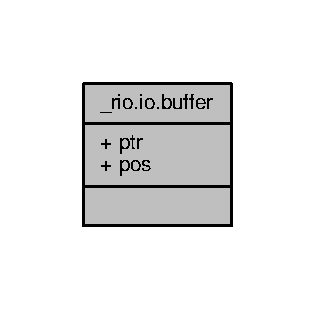
\includegraphics[width=151pt]{struct__rio_8io_8buffer__coll__graph}
\end{center}
\end{figure}
\subsection*{Data Fields}
\begin{DoxyCompactItemize}
\item 
\mbox{\Hypertarget{struct__rio_8io_8buffer_a4d9ad2b37053671b594b237bd061b3f2}\label{struct__rio_8io_8buffer_a4d9ad2b37053671b594b237bd061b3f2}} 
sds {\bfseries ptr}
\item 
\mbox{\Hypertarget{struct__rio_8io_8buffer_a5e0bdcbddccca4d66d74ba8c1cee1a68}\label{struct__rio_8io_8buffer_a5e0bdcbddccca4d66d74ba8c1cee1a68}} 
off\+\_\+t {\bfseries pos}
\end{DoxyCompactItemize}


\subsection{Detailed Description}


Definition at line \hyperlink{rio_8h_source_l00066}{66} of file \hyperlink{rio_8h_source}{rio.\+h}.



\subsection{Field Documentation}
\mbox{\Hypertarget{struct__rio_8io_8buffer_a5e0bdcbddccca4d66d74ba8c1cee1a68}\label{struct__rio_8io_8buffer_a5e0bdcbddccca4d66d74ba8c1cee1a68}} 
\index{\+\_\+rio.\+io.\+buffer@{\+\_\+rio.\+io.\+buffer}!pos@{pos}}
\index{pos@{pos}!\+\_\+rio.\+io.\+buffer@{\+\_\+rio.\+io.\+buffer}}
\subsubsection{\texorpdfstring{pos}{pos}}
{\footnotesize\ttfamily }

\mbox{\Hypertarget{struct__rio_8io_8buffer_a4d9ad2b37053671b594b237bd061b3f2}\label{struct__rio_8io_8buffer_a4d9ad2b37053671b594b237bd061b3f2}} 
\index{\+\_\+rio.\+io.\+buffer@{\+\_\+rio.\+io.\+buffer}!ptr@{ptr}}
\index{ptr@{ptr}!\+\_\+rio.\+io.\+buffer@{\+\_\+rio.\+io.\+buffer}}
\subsubsection{\texorpdfstring{ptr}{ptr}}
{\footnotesize\ttfamily }



The documentation for this struct was generated from the following files\+:
\hypertarget{struct__rio_8io_8fdset}{}\section{\+\_\+rio.\+io.\+fdset Struct Reference}
\label{struct__rio_8io_8fdset}\index{\+\_\+rio.\+io.\+fdset@{\+\_\+rio.\+io.\+fdset}}


Collaboration diagram for \+\_\+rio.\+io.\+fdset\+:\nopagebreak
\begin{figure}[H]
\begin{center}
\leavevmode
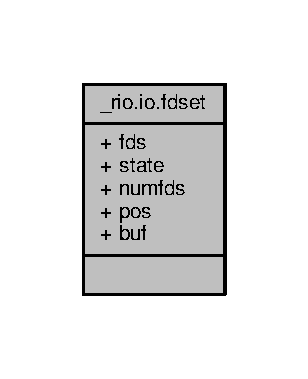
\includegraphics[width=148pt]{struct__rio_8io_8fdset__coll__graph}
\end{center}
\end{figure}
\subsection*{Data Fields}
\begin{DoxyCompactItemize}
\item 
\mbox{\Hypertarget{struct__rio_8io_8fdset_a838ece1033bf7c7468e873e79ba2a3ec}\label{struct__rio_8io_8fdset_a838ece1033bf7c7468e873e79ba2a3ec}} 
int $\ast$ {\bfseries fds}
\item 
\mbox{\Hypertarget{struct__rio_8io_8fdset_a9ed39e2ea931586b6a985a6942ef573e}\label{struct__rio_8io_8fdset_a9ed39e2ea931586b6a985a6942ef573e}} 
int $\ast$ {\bfseries state}
\item 
\mbox{\Hypertarget{struct__rio_8io_8fdset_a7b140b149c75a21ccb7ba8f6fe4dd7fc}\label{struct__rio_8io_8fdset_a7b140b149c75a21ccb7ba8f6fe4dd7fc}} 
int {\bfseries numfds}
\item 
\mbox{\Hypertarget{struct__rio_8io_8fdset_a5e0bdcbddccca4d66d74ba8c1cee1a68}\label{struct__rio_8io_8fdset_a5e0bdcbddccca4d66d74ba8c1cee1a68}} 
off\+\_\+t {\bfseries pos}
\item 
\mbox{\Hypertarget{struct__rio_8io_8fdset_acb7e52b21171fb9a53b498202607f0bd}\label{struct__rio_8io_8fdset_acb7e52b21171fb9a53b498202607f0bd}} 
sds {\bfseries buf}
\end{DoxyCompactItemize}


\subsection{Detailed Description}


Definition at line \hyperlink{rio_8h_source_l00077}{77} of file \hyperlink{rio_8h_source}{rio.\+h}.



\subsection{Field Documentation}
\mbox{\Hypertarget{struct__rio_8io_8fdset_acb7e52b21171fb9a53b498202607f0bd}\label{struct__rio_8io_8fdset_acb7e52b21171fb9a53b498202607f0bd}} 
\index{\+\_\+rio.\+io.\+fdset@{\+\_\+rio.\+io.\+fdset}!buf@{buf}}
\index{buf@{buf}!\+\_\+rio.\+io.\+fdset@{\+\_\+rio.\+io.\+fdset}}
\subsubsection{\texorpdfstring{buf}{buf}}
{\footnotesize\ttfamily }

\mbox{\Hypertarget{struct__rio_8io_8fdset_a838ece1033bf7c7468e873e79ba2a3ec}\label{struct__rio_8io_8fdset_a838ece1033bf7c7468e873e79ba2a3ec}} 
\index{\+\_\+rio.\+io.\+fdset@{\+\_\+rio.\+io.\+fdset}!fds@{fds}}
\index{fds@{fds}!\+\_\+rio.\+io.\+fdset@{\+\_\+rio.\+io.\+fdset}}
\subsubsection{\texorpdfstring{fds}{fds}}
{\footnotesize\ttfamily }

\mbox{\Hypertarget{struct__rio_8io_8fdset_a7b140b149c75a21ccb7ba8f6fe4dd7fc}\label{struct__rio_8io_8fdset_a7b140b149c75a21ccb7ba8f6fe4dd7fc}} 
\index{\+\_\+rio.\+io.\+fdset@{\+\_\+rio.\+io.\+fdset}!numfds@{numfds}}
\index{numfds@{numfds}!\+\_\+rio.\+io.\+fdset@{\+\_\+rio.\+io.\+fdset}}
\subsubsection{\texorpdfstring{numfds}{numfds}}
{\footnotesize\ttfamily }

\mbox{\Hypertarget{struct__rio_8io_8fdset_a5e0bdcbddccca4d66d74ba8c1cee1a68}\label{struct__rio_8io_8fdset_a5e0bdcbddccca4d66d74ba8c1cee1a68}} 
\index{\+\_\+rio.\+io.\+fdset@{\+\_\+rio.\+io.\+fdset}!pos@{pos}}
\index{pos@{pos}!\+\_\+rio.\+io.\+fdset@{\+\_\+rio.\+io.\+fdset}}
\subsubsection{\texorpdfstring{pos}{pos}}
{\footnotesize\ttfamily }

\mbox{\Hypertarget{struct__rio_8io_8fdset_a9ed39e2ea931586b6a985a6942ef573e}\label{struct__rio_8io_8fdset_a9ed39e2ea931586b6a985a6942ef573e}} 
\index{\+\_\+rio.\+io.\+fdset@{\+\_\+rio.\+io.\+fdset}!state@{state}}
\index{state@{state}!\+\_\+rio.\+io.\+fdset@{\+\_\+rio.\+io.\+fdset}}
\subsubsection{\texorpdfstring{state}{state}}
{\footnotesize\ttfamily }



The documentation for this struct was generated from the following files\+:
\hypertarget{struct__rio_8io_8file}{}\section{\+\_\+rio.\+io.\+file Struct Reference}
\label{struct__rio_8io_8file}\index{\+\_\+rio.\+io.\+file@{\+\_\+rio.\+io.\+file}}


Collaboration diagram for \+\_\+rio.\+io.\+file\+:\nopagebreak
\begin{figure}[H]
\begin{center}
\leavevmode
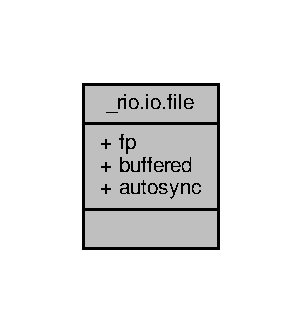
\includegraphics[width=145pt]{struct__rio_8io_8file__coll__graph}
\end{center}
\end{figure}
\subsection*{Data Fields}
\begin{DoxyCompactItemize}
\item 
\mbox{\Hypertarget{struct__rio_8io_8file_a0666f0acdeed38d4cd9084ade1739498}\label{struct__rio_8io_8file_a0666f0acdeed38d4cd9084ade1739498}} 
F\+I\+LE $\ast$ {\bfseries fp}
\item 
\mbox{\Hypertarget{struct__rio_8io_8file_a8b365ffbd5d92a1b9c20f227a4b6fcec}\label{struct__rio_8io_8file_a8b365ffbd5d92a1b9c20f227a4b6fcec}} 
off\+\_\+t {\bfseries buffered}
\item 
\mbox{\Hypertarget{struct__rio_8io_8file_a7436fa807f1e0acb8fe0541598ad3ab1}\label{struct__rio_8io_8file_a7436fa807f1e0acb8fe0541598ad3ab1}} 
off\+\_\+t {\bfseries autosync}
\end{DoxyCompactItemize}


\subsection{Detailed Description}


Definition at line \hyperlink{rio_8h_source_l00071}{71} of file \hyperlink{rio_8h_source}{rio.\+h}.



\subsection{Field Documentation}
\mbox{\Hypertarget{struct__rio_8io_8file_a7436fa807f1e0acb8fe0541598ad3ab1}\label{struct__rio_8io_8file_a7436fa807f1e0acb8fe0541598ad3ab1}} 
\index{\+\_\+rio.\+io.\+file@{\+\_\+rio.\+io.\+file}!autosync@{autosync}}
\index{autosync@{autosync}!\+\_\+rio.\+io.\+file@{\+\_\+rio.\+io.\+file}}
\subsubsection{\texorpdfstring{autosync}{autosync}}
{\footnotesize\ttfamily }

\mbox{\Hypertarget{struct__rio_8io_8file_a8b365ffbd5d92a1b9c20f227a4b6fcec}\label{struct__rio_8io_8file_a8b365ffbd5d92a1b9c20f227a4b6fcec}} 
\index{\+\_\+rio.\+io.\+file@{\+\_\+rio.\+io.\+file}!buffered@{buffered}}
\index{buffered@{buffered}!\+\_\+rio.\+io.\+file@{\+\_\+rio.\+io.\+file}}
\subsubsection{\texorpdfstring{buffered}{buffered}}
{\footnotesize\ttfamily }

\mbox{\Hypertarget{struct__rio_8io_8file_a0666f0acdeed38d4cd9084ade1739498}\label{struct__rio_8io_8file_a0666f0acdeed38d4cd9084ade1739498}} 
\index{\+\_\+rio.\+io.\+file@{\+\_\+rio.\+io.\+file}!fp@{fp}}
\index{fp@{fp}!\+\_\+rio.\+io.\+file@{\+\_\+rio.\+io.\+file}}
\subsubsection{\texorpdfstring{fp}{fp}}
{\footnotesize\ttfamily }



The documentation for this struct was generated from the following files\+:
\hypertarget{structaeApiState}{}\section{ae\+Api\+State Struct Reference}
\label{structaeApiState}\index{ae\+Api\+State@{ae\+Api\+State}}


Collaboration diagram for ae\+Api\+State\+:\nopagebreak
\begin{figure}[H]
\begin{center}
\leavevmode
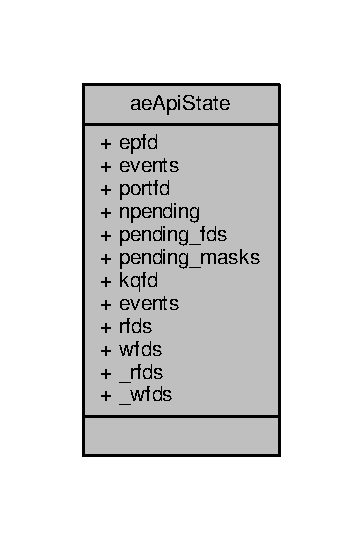
\includegraphics[width=174pt]{structaeApiState__coll__graph}
\end{center}
\end{figure}
\subsection*{Data Fields}
\begin{DoxyCompactItemize}
\item 
\mbox{\Hypertarget{structaeApiState_ad22cb6aa093b0606521178bee5fc9e57}\label{structaeApiState_ad22cb6aa093b0606521178bee5fc9e57}} 
int {\bfseries epfd}
\item 
\mbox{\Hypertarget{structaeApiState_aae9919a5fbc7f635b7add5e9afca911f}\label{structaeApiState_aae9919a5fbc7f635b7add5e9afca911f}} 
struct epoll\+\_\+event $\ast$ {\bfseries events}
\item 
\mbox{\Hypertarget{structaeApiState_a03b5c6f2f76f6817b516078a80132322}\label{structaeApiState_a03b5c6f2f76f6817b516078a80132322}} 
int {\bfseries portfd}
\item 
\mbox{\Hypertarget{structaeApiState_a4adaf2e0c58326bb1fb58f9dff2010f6}\label{structaeApiState_a4adaf2e0c58326bb1fb58f9dff2010f6}} 
int {\bfseries npending}
\item 
\mbox{\Hypertarget{structaeApiState_afd83ec51c15792c39367389a247b43b5}\label{structaeApiState_afd83ec51c15792c39367389a247b43b5}} 
int {\bfseries pending\+\_\+fds} \mbox{[}M\+A\+X\+\_\+\+E\+V\+E\+N\+T\+\_\+\+B\+A\+T\+C\+H\+SZ\mbox{]}
\item 
\mbox{\Hypertarget{structaeApiState_a6ee1e116dccf9bf2a1bd466226ff6dfa}\label{structaeApiState_a6ee1e116dccf9bf2a1bd466226ff6dfa}} 
int {\bfseries pending\+\_\+masks} \mbox{[}M\+A\+X\+\_\+\+E\+V\+E\+N\+T\+\_\+\+B\+A\+T\+C\+H\+SZ\mbox{]}
\item 
\mbox{\Hypertarget{structaeApiState_a091974c7b256e357ff535ce63012ff84}\label{structaeApiState_a091974c7b256e357ff535ce63012ff84}} 
int {\bfseries kqfd}
\item 
\mbox{\Hypertarget{structaeApiState_a3dad05e80c97db4396002b7e77e02c9c}\label{structaeApiState_a3dad05e80c97db4396002b7e77e02c9c}} 
struct kevent $\ast$ {\bfseries events}
\item 
\mbox{\Hypertarget{structaeApiState_a3faa88b3bb101d3f8879a4c167a553d8}\label{structaeApiState_a3faa88b3bb101d3f8879a4c167a553d8}} 
fd\+\_\+set {\bfseries rfds}
\item 
\mbox{\Hypertarget{structaeApiState_a5e0a54365408102a313690971e9e6d95}\label{structaeApiState_a5e0a54365408102a313690971e9e6d95}} 
fd\+\_\+set {\bfseries wfds}
\item 
\mbox{\Hypertarget{structaeApiState_ab9820d1695885949ecf0d2ce687a8568}\label{structaeApiState_ab9820d1695885949ecf0d2ce687a8568}} 
fd\+\_\+set {\bfseries \+\_\+rfds}
\item 
\mbox{\Hypertarget{structaeApiState_a112ee06858937f805534a328e3620327}\label{structaeApiState_a112ee06858937f805534a328e3620327}} 
fd\+\_\+set {\bfseries \+\_\+wfds}
\end{DoxyCompactItemize}


\subsection{Detailed Description}


Definition at line \hyperlink{ae__epoll_8c_source_l00034}{34} of file \hyperlink{ae__epoll_8c_source}{ae\+\_\+epoll.\+c}.



\subsection{Field Documentation}
\mbox{\Hypertarget{structaeApiState_ab9820d1695885949ecf0d2ce687a8568}\label{structaeApiState_ab9820d1695885949ecf0d2ce687a8568}} 
\index{ae\+Api\+State@{ae\+Api\+State}!\+\_\+rfds@{\+\_\+rfds}}
\index{\+\_\+rfds@{\+\_\+rfds}!ae\+Api\+State@{ae\+Api\+State}}
\subsubsection{\texorpdfstring{\+\_\+rfds}{\_rfds}}
{\footnotesize\ttfamily fd\+\_\+set ae\+Api\+State\+::\+\_\+rfds}



Definition at line \hyperlink{ae__select_8c_source_l00039}{39} of file \hyperlink{ae__select_8c_source}{ae\+\_\+select.\+c}.

\mbox{\Hypertarget{structaeApiState_a112ee06858937f805534a328e3620327}\label{structaeApiState_a112ee06858937f805534a328e3620327}} 
\index{ae\+Api\+State@{ae\+Api\+State}!\+\_\+wfds@{\+\_\+wfds}}
\index{\+\_\+wfds@{\+\_\+wfds}!ae\+Api\+State@{ae\+Api\+State}}
\subsubsection{\texorpdfstring{\+\_\+wfds}{\_wfds}}
{\footnotesize\ttfamily fd\+\_\+set ae\+Api\+State\+::\+\_\+wfds}



Definition at line \hyperlink{ae__select_8c_source_l00039}{39} of file \hyperlink{ae__select_8c_source}{ae\+\_\+select.\+c}.

\mbox{\Hypertarget{structaeApiState_ad22cb6aa093b0606521178bee5fc9e57}\label{structaeApiState_ad22cb6aa093b0606521178bee5fc9e57}} 
\index{ae\+Api\+State@{ae\+Api\+State}!epfd@{epfd}}
\index{epfd@{epfd}!ae\+Api\+State@{ae\+Api\+State}}
\subsubsection{\texorpdfstring{epfd}{epfd}}
{\footnotesize\ttfamily int ae\+Api\+State\+::epfd}



Definition at line \hyperlink{ae__epoll_8c_source_l00035}{35} of file \hyperlink{ae__epoll_8c_source}{ae\+\_\+epoll.\+c}.

\mbox{\Hypertarget{structaeApiState_aae9919a5fbc7f635b7add5e9afca911f}\label{structaeApiState_aae9919a5fbc7f635b7add5e9afca911f}} 
\index{ae\+Api\+State@{ae\+Api\+State}!events@{events}}
\index{events@{events}!ae\+Api\+State@{ae\+Api\+State}}
\subsubsection{\texorpdfstring{events}{events}\hspace{0.1cm}{\footnotesize\ttfamily [1/2]}}
{\footnotesize\ttfamily struct epoll\+\_\+event$\ast$ ae\+Api\+State\+::events}



Definition at line \hyperlink{ae__epoll_8c_source_l00036}{36} of file \hyperlink{ae__epoll_8c_source}{ae\+\_\+epoll.\+c}.

\mbox{\Hypertarget{structaeApiState_a3dad05e80c97db4396002b7e77e02c9c}\label{structaeApiState_a3dad05e80c97db4396002b7e77e02c9c}} 
\index{ae\+Api\+State@{ae\+Api\+State}!events@{events}}
\index{events@{events}!ae\+Api\+State@{ae\+Api\+State}}
\subsubsection{\texorpdfstring{events}{events}\hspace{0.1cm}{\footnotesize\ttfamily [2/2]}}
{\footnotesize\ttfamily struct kevent$\ast$ ae\+Api\+State\+::events}



Definition at line \hyperlink{ae__kqueue_8c_source_l00038}{38} of file \hyperlink{ae__kqueue_8c_source}{ae\+\_\+kqueue.\+c}.

\mbox{\Hypertarget{structaeApiState_a091974c7b256e357ff535ce63012ff84}\label{structaeApiState_a091974c7b256e357ff535ce63012ff84}} 
\index{ae\+Api\+State@{ae\+Api\+State}!kqfd@{kqfd}}
\index{kqfd@{kqfd}!ae\+Api\+State@{ae\+Api\+State}}
\subsubsection{\texorpdfstring{kqfd}{kqfd}}
{\footnotesize\ttfamily int ae\+Api\+State\+::kqfd}



Definition at line \hyperlink{ae__kqueue_8c_source_l00037}{37} of file \hyperlink{ae__kqueue_8c_source}{ae\+\_\+kqueue.\+c}.

\mbox{\Hypertarget{structaeApiState_a4adaf2e0c58326bb1fb58f9dff2010f6}\label{structaeApiState_a4adaf2e0c58326bb1fb58f9dff2010f6}} 
\index{ae\+Api\+State@{ae\+Api\+State}!npending@{npending}}
\index{npending@{npending}!ae\+Api\+State@{ae\+Api\+State}}
\subsubsection{\texorpdfstring{npending}{npending}}
{\footnotesize\ttfamily int ae\+Api\+State\+::npending}



Definition at line \hyperlink{ae__evport_8c_source_l00070}{70} of file \hyperlink{ae__evport_8c_source}{ae\+\_\+evport.\+c}.

\mbox{\Hypertarget{structaeApiState_afd83ec51c15792c39367389a247b43b5}\label{structaeApiState_afd83ec51c15792c39367389a247b43b5}} 
\index{ae\+Api\+State@{ae\+Api\+State}!pending\+\_\+fds@{pending\+\_\+fds}}
\index{pending\+\_\+fds@{pending\+\_\+fds}!ae\+Api\+State@{ae\+Api\+State}}
\subsubsection{\texorpdfstring{pending\+\_\+fds}{pending\_fds}}
{\footnotesize\ttfamily int ae\+Api\+State\+::pending\+\_\+fds\mbox{[}M\+A\+X\+\_\+\+E\+V\+E\+N\+T\+\_\+\+B\+A\+T\+C\+H\+SZ\mbox{]}}



Definition at line \hyperlink{ae__evport_8c_source_l00071}{71} of file \hyperlink{ae__evport_8c_source}{ae\+\_\+evport.\+c}.

\mbox{\Hypertarget{structaeApiState_a6ee1e116dccf9bf2a1bd466226ff6dfa}\label{structaeApiState_a6ee1e116dccf9bf2a1bd466226ff6dfa}} 
\index{ae\+Api\+State@{ae\+Api\+State}!pending\+\_\+masks@{pending\+\_\+masks}}
\index{pending\+\_\+masks@{pending\+\_\+masks}!ae\+Api\+State@{ae\+Api\+State}}
\subsubsection{\texorpdfstring{pending\+\_\+masks}{pending\_masks}}
{\footnotesize\ttfamily int ae\+Api\+State\+::pending\+\_\+masks\mbox{[}M\+A\+X\+\_\+\+E\+V\+E\+N\+T\+\_\+\+B\+A\+T\+C\+H\+SZ\mbox{]}}



Definition at line \hyperlink{ae__evport_8c_source_l00072}{72} of file \hyperlink{ae__evport_8c_source}{ae\+\_\+evport.\+c}.

\mbox{\Hypertarget{structaeApiState_a03b5c6f2f76f6817b516078a80132322}\label{structaeApiState_a03b5c6f2f76f6817b516078a80132322}} 
\index{ae\+Api\+State@{ae\+Api\+State}!portfd@{portfd}}
\index{portfd@{portfd}!ae\+Api\+State@{ae\+Api\+State}}
\subsubsection{\texorpdfstring{portfd}{portfd}}
{\footnotesize\ttfamily int ae\+Api\+State\+::portfd}



Definition at line \hyperlink{ae__evport_8c_source_l00069}{69} of file \hyperlink{ae__evport_8c_source}{ae\+\_\+evport.\+c}.

\mbox{\Hypertarget{structaeApiState_a3faa88b3bb101d3f8879a4c167a553d8}\label{structaeApiState_a3faa88b3bb101d3f8879a4c167a553d8}} 
\index{ae\+Api\+State@{ae\+Api\+State}!rfds@{rfds}}
\index{rfds@{rfds}!ae\+Api\+State@{ae\+Api\+State}}
\subsubsection{\texorpdfstring{rfds}{rfds}}
{\footnotesize\ttfamily fd\+\_\+set ae\+Api\+State\+::rfds}



Definition at line \hyperlink{ae__select_8c_source_l00036}{36} of file \hyperlink{ae__select_8c_source}{ae\+\_\+select.\+c}.

\mbox{\Hypertarget{structaeApiState_a5e0a54365408102a313690971e9e6d95}\label{structaeApiState_a5e0a54365408102a313690971e9e6d95}} 
\index{ae\+Api\+State@{ae\+Api\+State}!wfds@{wfds}}
\index{wfds@{wfds}!ae\+Api\+State@{ae\+Api\+State}}
\subsubsection{\texorpdfstring{wfds}{wfds}}
{\footnotesize\ttfamily fd\+\_\+set ae\+Api\+State\+::wfds}



Definition at line \hyperlink{ae__select_8c_source_l00036}{36} of file \hyperlink{ae__select_8c_source}{ae\+\_\+select.\+c}.



The documentation for this struct was generated from the following files\+:\begin{DoxyCompactItemize}
\item 
src/ae\+\_\+epoll.\+c\item 
src/ae\+\_\+evport.\+c\item 
src/ae\+\_\+kqueue.\+c\item 
src/ae\+\_\+select.\+c\end{DoxyCompactItemize}

\hypertarget{structaeEventLoop}{}\section{ae\+Event\+Loop Struct Reference}
\label{structaeEventLoop}\index{ae\+Event\+Loop@{ae\+Event\+Loop}}


Collaboration diagram for ae\+Event\+Loop\+:\nopagebreak
\begin{figure}[H]
\begin{center}
\leavevmode
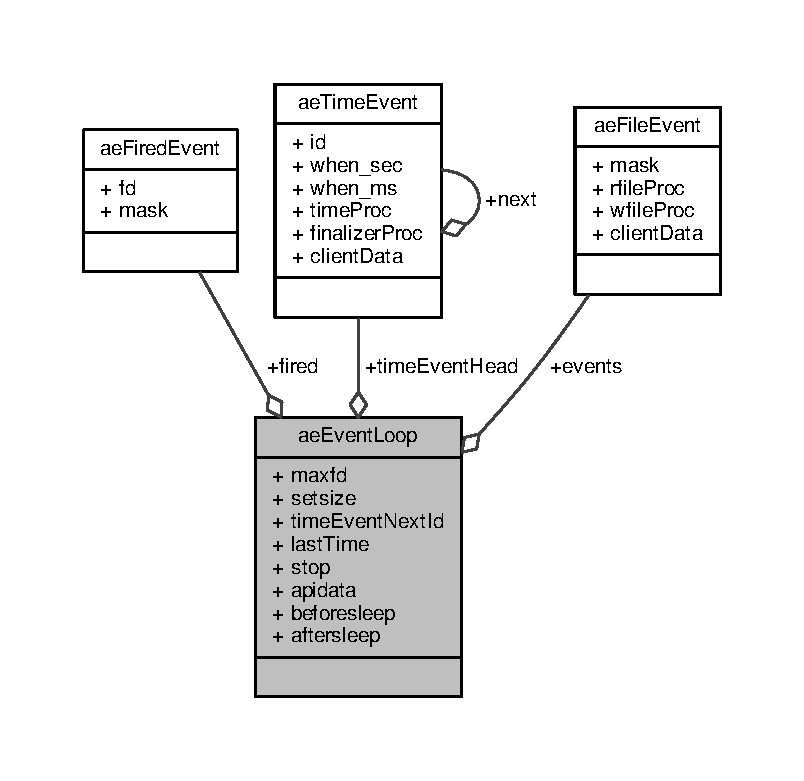
\includegraphics[width=350pt]{structaeEventLoop__coll__graph}
\end{center}
\end{figure}
\subsection*{Data Fields}
\begin{DoxyCompactItemize}
\item 
\mbox{\Hypertarget{structaeEventLoop_aedf39e37f559c83d9a0ae1ae07e5b8c1}\label{structaeEventLoop_aedf39e37f559c83d9a0ae1ae07e5b8c1}} 
int {\bfseries maxfd}
\item 
\mbox{\Hypertarget{structaeEventLoop_a319d48af757c6f6144fa4066994f6541}\label{structaeEventLoop_a319d48af757c6f6144fa4066994f6541}} 
int {\bfseries setsize}
\item 
\mbox{\Hypertarget{structaeEventLoop_a9c389db589e8e0118be0c753c0eed909}\label{structaeEventLoop_a9c389db589e8e0118be0c753c0eed909}} 
long long {\bfseries time\+Event\+Next\+Id}
\item 
\mbox{\Hypertarget{structaeEventLoop_aead81eebbc8104bef63d9372fabc1b61}\label{structaeEventLoop_aead81eebbc8104bef63d9372fabc1b61}} 
time\+\_\+t {\bfseries last\+Time}
\item 
\mbox{\Hypertarget{structaeEventLoop_aa37dcf314ec826fafa4b3ff05923b434}\label{structaeEventLoop_aa37dcf314ec826fafa4b3ff05923b434}} 
\hyperlink{structaeFileEvent}{ae\+File\+Event} $\ast$ {\bfseries events}
\item 
\mbox{\Hypertarget{structaeEventLoop_aa2ccda94b3ee8a43a4802bd1f8443609}\label{structaeEventLoop_aa2ccda94b3ee8a43a4802bd1f8443609}} 
\hyperlink{structaeFiredEvent}{ae\+Fired\+Event} $\ast$ {\bfseries fired}
\item 
\mbox{\Hypertarget{structaeEventLoop_a2c992f66acb2ba2d1d13890c55008788}\label{structaeEventLoop_a2c992f66acb2ba2d1d13890c55008788}} 
\hyperlink{structaeTimeEvent}{ae\+Time\+Event} $\ast$ {\bfseries time\+Event\+Head}
\item 
\mbox{\Hypertarget{structaeEventLoop_a79b39021b2e805b8a547915d22279168}\label{structaeEventLoop_a79b39021b2e805b8a547915d22279168}} 
int {\bfseries stop}
\item 
\mbox{\Hypertarget{structaeEventLoop_a6e5405d4ffa2492794fa74ee4cf6fb49}\label{structaeEventLoop_a6e5405d4ffa2492794fa74ee4cf6fb49}} 
void $\ast$ {\bfseries apidata}
\item 
\mbox{\Hypertarget{structaeEventLoop_ae65cc21b6c2f11a2de8e6e62fa660a79}\label{structaeEventLoop_ae65cc21b6c2f11a2de8e6e62fa660a79}} 
ae\+Before\+Sleep\+Proc $\ast$ {\bfseries beforesleep}
\item 
\mbox{\Hypertarget{structaeEventLoop_ae28e7719da59d474c1aa85527ab744e9}\label{structaeEventLoop_ae28e7719da59d474c1aa85527ab744e9}} 
ae\+Before\+Sleep\+Proc $\ast$ {\bfseries aftersleep}
\end{DoxyCompactItemize}


\subsection{Detailed Description}


Definition at line \hyperlink{ae_8h_source_l00091}{91} of file \hyperlink{ae_8h_source}{ae.\+h}.



\subsection{Field Documentation}
\mbox{\Hypertarget{structaeEventLoop_ae28e7719da59d474c1aa85527ab744e9}\label{structaeEventLoop_ae28e7719da59d474c1aa85527ab744e9}} 
\index{ae\+Event\+Loop@{ae\+Event\+Loop}!aftersleep@{aftersleep}}
\index{aftersleep@{aftersleep}!ae\+Event\+Loop@{ae\+Event\+Loop}}
\subsubsection{\texorpdfstring{aftersleep}{aftersleep}}
{\footnotesize\ttfamily ae\+Before\+Sleep\+Proc$\ast$ ae\+Event\+Loop\+::aftersleep}



Definition at line \hyperlink{ae_8h_source_l00102}{102} of file \hyperlink{ae_8h_source}{ae.\+h}.

\mbox{\Hypertarget{structaeEventLoop_a6e5405d4ffa2492794fa74ee4cf6fb49}\label{structaeEventLoop_a6e5405d4ffa2492794fa74ee4cf6fb49}} 
\index{ae\+Event\+Loop@{ae\+Event\+Loop}!apidata@{apidata}}
\index{apidata@{apidata}!ae\+Event\+Loop@{ae\+Event\+Loop}}
\subsubsection{\texorpdfstring{apidata}{apidata}}
{\footnotesize\ttfamily void$\ast$ ae\+Event\+Loop\+::apidata}



Definition at line \hyperlink{ae_8h_source_l00100}{100} of file \hyperlink{ae_8h_source}{ae.\+h}.

\mbox{\Hypertarget{structaeEventLoop_ae65cc21b6c2f11a2de8e6e62fa660a79}\label{structaeEventLoop_ae65cc21b6c2f11a2de8e6e62fa660a79}} 
\index{ae\+Event\+Loop@{ae\+Event\+Loop}!beforesleep@{beforesleep}}
\index{beforesleep@{beforesleep}!ae\+Event\+Loop@{ae\+Event\+Loop}}
\subsubsection{\texorpdfstring{beforesleep}{beforesleep}}
{\footnotesize\ttfamily ae\+Before\+Sleep\+Proc$\ast$ ae\+Event\+Loop\+::beforesleep}



Definition at line \hyperlink{ae_8h_source_l00101}{101} of file \hyperlink{ae_8h_source}{ae.\+h}.

\mbox{\Hypertarget{structaeEventLoop_aa37dcf314ec826fafa4b3ff05923b434}\label{structaeEventLoop_aa37dcf314ec826fafa4b3ff05923b434}} 
\index{ae\+Event\+Loop@{ae\+Event\+Loop}!events@{events}}
\index{events@{events}!ae\+Event\+Loop@{ae\+Event\+Loop}}
\subsubsection{\texorpdfstring{events}{events}}
{\footnotesize\ttfamily \hyperlink{structaeFileEvent}{ae\+File\+Event}$\ast$ ae\+Event\+Loop\+::events}



Definition at line \hyperlink{ae_8h_source_l00096}{96} of file \hyperlink{ae_8h_source}{ae.\+h}.

\mbox{\Hypertarget{structaeEventLoop_aa2ccda94b3ee8a43a4802bd1f8443609}\label{structaeEventLoop_aa2ccda94b3ee8a43a4802bd1f8443609}} 
\index{ae\+Event\+Loop@{ae\+Event\+Loop}!fired@{fired}}
\index{fired@{fired}!ae\+Event\+Loop@{ae\+Event\+Loop}}
\subsubsection{\texorpdfstring{fired}{fired}}
{\footnotesize\ttfamily \hyperlink{structaeFiredEvent}{ae\+Fired\+Event}$\ast$ ae\+Event\+Loop\+::fired}



Definition at line \hyperlink{ae_8h_source_l00097}{97} of file \hyperlink{ae_8h_source}{ae.\+h}.

\mbox{\Hypertarget{structaeEventLoop_aead81eebbc8104bef63d9372fabc1b61}\label{structaeEventLoop_aead81eebbc8104bef63d9372fabc1b61}} 
\index{ae\+Event\+Loop@{ae\+Event\+Loop}!last\+Time@{last\+Time}}
\index{last\+Time@{last\+Time}!ae\+Event\+Loop@{ae\+Event\+Loop}}
\subsubsection{\texorpdfstring{last\+Time}{lastTime}}
{\footnotesize\ttfamily time\+\_\+t ae\+Event\+Loop\+::last\+Time}



Definition at line \hyperlink{ae_8h_source_l00095}{95} of file \hyperlink{ae_8h_source}{ae.\+h}.

\mbox{\Hypertarget{structaeEventLoop_aedf39e37f559c83d9a0ae1ae07e5b8c1}\label{structaeEventLoop_aedf39e37f559c83d9a0ae1ae07e5b8c1}} 
\index{ae\+Event\+Loop@{ae\+Event\+Loop}!maxfd@{maxfd}}
\index{maxfd@{maxfd}!ae\+Event\+Loop@{ae\+Event\+Loop}}
\subsubsection{\texorpdfstring{maxfd}{maxfd}}
{\footnotesize\ttfamily int ae\+Event\+Loop\+::maxfd}



Definition at line \hyperlink{ae_8h_source_l00092}{92} of file \hyperlink{ae_8h_source}{ae.\+h}.

\mbox{\Hypertarget{structaeEventLoop_a319d48af757c6f6144fa4066994f6541}\label{structaeEventLoop_a319d48af757c6f6144fa4066994f6541}} 
\index{ae\+Event\+Loop@{ae\+Event\+Loop}!setsize@{setsize}}
\index{setsize@{setsize}!ae\+Event\+Loop@{ae\+Event\+Loop}}
\subsubsection{\texorpdfstring{setsize}{setsize}}
{\footnotesize\ttfamily int ae\+Event\+Loop\+::setsize}



Definition at line \hyperlink{ae_8h_source_l00093}{93} of file \hyperlink{ae_8h_source}{ae.\+h}.

\mbox{\Hypertarget{structaeEventLoop_a79b39021b2e805b8a547915d22279168}\label{structaeEventLoop_a79b39021b2e805b8a547915d22279168}} 
\index{ae\+Event\+Loop@{ae\+Event\+Loop}!stop@{stop}}
\index{stop@{stop}!ae\+Event\+Loop@{ae\+Event\+Loop}}
\subsubsection{\texorpdfstring{stop}{stop}}
{\footnotesize\ttfamily int ae\+Event\+Loop\+::stop}



Definition at line \hyperlink{ae_8h_source_l00099}{99} of file \hyperlink{ae_8h_source}{ae.\+h}.

\mbox{\Hypertarget{structaeEventLoop_a2c992f66acb2ba2d1d13890c55008788}\label{structaeEventLoop_a2c992f66acb2ba2d1d13890c55008788}} 
\index{ae\+Event\+Loop@{ae\+Event\+Loop}!time\+Event\+Head@{time\+Event\+Head}}
\index{time\+Event\+Head@{time\+Event\+Head}!ae\+Event\+Loop@{ae\+Event\+Loop}}
\subsubsection{\texorpdfstring{time\+Event\+Head}{timeEventHead}}
{\footnotesize\ttfamily \hyperlink{structaeTimeEvent}{ae\+Time\+Event}$\ast$ ae\+Event\+Loop\+::time\+Event\+Head}



Definition at line \hyperlink{ae_8h_source_l00098}{98} of file \hyperlink{ae_8h_source}{ae.\+h}.

\mbox{\Hypertarget{structaeEventLoop_a9c389db589e8e0118be0c753c0eed909}\label{structaeEventLoop_a9c389db589e8e0118be0c753c0eed909}} 
\index{ae\+Event\+Loop@{ae\+Event\+Loop}!time\+Event\+Next\+Id@{time\+Event\+Next\+Id}}
\index{time\+Event\+Next\+Id@{time\+Event\+Next\+Id}!ae\+Event\+Loop@{ae\+Event\+Loop}}
\subsubsection{\texorpdfstring{time\+Event\+Next\+Id}{timeEventNextId}}
{\footnotesize\ttfamily long long ae\+Event\+Loop\+::time\+Event\+Next\+Id}



Definition at line \hyperlink{ae_8h_source_l00094}{94} of file \hyperlink{ae_8h_source}{ae.\+h}.



The documentation for this struct was generated from the following file\+:\begin{DoxyCompactItemize}
\item 
src/ae.\+h\end{DoxyCompactItemize}

\hypertarget{structaeFileEvent}{}\section{ae\+File\+Event Struct Reference}
\label{structaeFileEvent}\index{ae\+File\+Event@{ae\+File\+Event}}


Collaboration diagram for ae\+File\+Event\+:\nopagebreak
\begin{figure}[H]
\begin{center}
\leavevmode
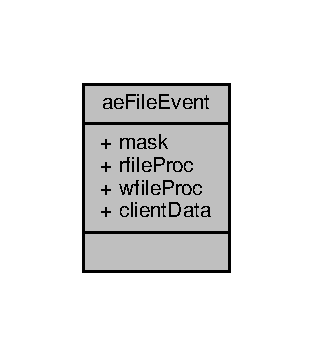
\includegraphics[width=150pt]{structaeFileEvent__coll__graph}
\end{center}
\end{figure}
\subsection*{Data Fields}
\begin{DoxyCompactItemize}
\item 
\mbox{\Hypertarget{structaeFileEvent_ac43aaab34810e8b6bfcc5a2576220959}\label{structaeFileEvent_ac43aaab34810e8b6bfcc5a2576220959}} 
int {\bfseries mask}
\item 
\mbox{\Hypertarget{structaeFileEvent_ae39bf42ed5c4cac998ee5c9fc4ee0069}\label{structaeFileEvent_ae39bf42ed5c4cac998ee5c9fc4ee0069}} 
ae\+File\+Proc $\ast$ {\bfseries rfile\+Proc}
\item 
\mbox{\Hypertarget{structaeFileEvent_a48ede39c4bcd4c41f2687efac2a05152}\label{structaeFileEvent_a48ede39c4bcd4c41f2687efac2a05152}} 
ae\+File\+Proc $\ast$ {\bfseries wfile\+Proc}
\item 
\mbox{\Hypertarget{structaeFileEvent_a001285b3f180bb6e776a97190fe47b7b}\label{structaeFileEvent_a001285b3f180bb6e776a97190fe47b7b}} 
void $\ast$ {\bfseries client\+Data}
\end{DoxyCompactItemize}


\subsection{Detailed Description}


Definition at line \hyperlink{ae_8h_source_l00066}{66} of file \hyperlink{ae_8h_source}{ae.\+h}.



\subsection{Field Documentation}
\mbox{\Hypertarget{structaeFileEvent_a001285b3f180bb6e776a97190fe47b7b}\label{structaeFileEvent_a001285b3f180bb6e776a97190fe47b7b}} 
\index{ae\+File\+Event@{ae\+File\+Event}!client\+Data@{client\+Data}}
\index{client\+Data@{client\+Data}!ae\+File\+Event@{ae\+File\+Event}}
\subsubsection{\texorpdfstring{client\+Data}{clientData}}
{\footnotesize\ttfamily void$\ast$ ae\+File\+Event\+::client\+Data}



Definition at line \hyperlink{ae_8h_source_l00070}{70} of file \hyperlink{ae_8h_source}{ae.\+h}.

\mbox{\Hypertarget{structaeFileEvent_ac43aaab34810e8b6bfcc5a2576220959}\label{structaeFileEvent_ac43aaab34810e8b6bfcc5a2576220959}} 
\index{ae\+File\+Event@{ae\+File\+Event}!mask@{mask}}
\index{mask@{mask}!ae\+File\+Event@{ae\+File\+Event}}
\subsubsection{\texorpdfstring{mask}{mask}}
{\footnotesize\ttfamily int ae\+File\+Event\+::mask}



Definition at line \hyperlink{ae_8h_source_l00067}{67} of file \hyperlink{ae_8h_source}{ae.\+h}.

\mbox{\Hypertarget{structaeFileEvent_ae39bf42ed5c4cac998ee5c9fc4ee0069}\label{structaeFileEvent_ae39bf42ed5c4cac998ee5c9fc4ee0069}} 
\index{ae\+File\+Event@{ae\+File\+Event}!rfile\+Proc@{rfile\+Proc}}
\index{rfile\+Proc@{rfile\+Proc}!ae\+File\+Event@{ae\+File\+Event}}
\subsubsection{\texorpdfstring{rfile\+Proc}{rfileProc}}
{\footnotesize\ttfamily ae\+File\+Proc$\ast$ ae\+File\+Event\+::rfile\+Proc}



Definition at line \hyperlink{ae_8h_source_l00068}{68} of file \hyperlink{ae_8h_source}{ae.\+h}.

\mbox{\Hypertarget{structaeFileEvent_a48ede39c4bcd4c41f2687efac2a05152}\label{structaeFileEvent_a48ede39c4bcd4c41f2687efac2a05152}} 
\index{ae\+File\+Event@{ae\+File\+Event}!wfile\+Proc@{wfile\+Proc}}
\index{wfile\+Proc@{wfile\+Proc}!ae\+File\+Event@{ae\+File\+Event}}
\subsubsection{\texorpdfstring{wfile\+Proc}{wfileProc}}
{\footnotesize\ttfamily ae\+File\+Proc$\ast$ ae\+File\+Event\+::wfile\+Proc}



Definition at line \hyperlink{ae_8h_source_l00069}{69} of file \hyperlink{ae_8h_source}{ae.\+h}.



The documentation for this struct was generated from the following file\+:\begin{DoxyCompactItemize}
\item 
src/ae.\+h\end{DoxyCompactItemize}

\hypertarget{structaeFiredEvent}{}\section{ae\+Fired\+Event Struct Reference}
\label{structaeFiredEvent}\index{ae\+Fired\+Event@{ae\+Fired\+Event}}


Collaboration diagram for ae\+Fired\+Event\+:\nopagebreak
\begin{figure}[H]
\begin{center}
\leavevmode
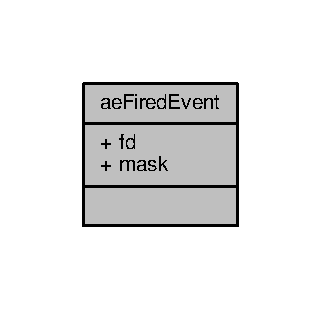
\includegraphics[width=154pt]{structaeFiredEvent__coll__graph}
\end{center}
\end{figure}
\subsection*{Data Fields}
\begin{DoxyCompactItemize}
\item 
\mbox{\Hypertarget{structaeFiredEvent_a66b9859d9d3004b412954713c6e213c6}\label{structaeFiredEvent_a66b9859d9d3004b412954713c6e213c6}} 
int {\bfseries fd}
\item 
\mbox{\Hypertarget{structaeFiredEvent_a2e9b1d9832d09a46c4a14e562aaa2aea}\label{structaeFiredEvent_a2e9b1d9832d09a46c4a14e562aaa2aea}} 
int {\bfseries mask}
\end{DoxyCompactItemize}


\subsection{Detailed Description}


Definition at line \hyperlink{ae_8h_source_l00085}{85} of file \hyperlink{ae_8h_source}{ae.\+h}.



\subsection{Field Documentation}
\mbox{\Hypertarget{structaeFiredEvent_a66b9859d9d3004b412954713c6e213c6}\label{structaeFiredEvent_a66b9859d9d3004b412954713c6e213c6}} 
\index{ae\+Fired\+Event@{ae\+Fired\+Event}!fd@{fd}}
\index{fd@{fd}!ae\+Fired\+Event@{ae\+Fired\+Event}}
\subsubsection{\texorpdfstring{fd}{fd}}
{\footnotesize\ttfamily int ae\+Fired\+Event\+::fd}



Definition at line \hyperlink{ae_8h_source_l00086}{86} of file \hyperlink{ae_8h_source}{ae.\+h}.

\mbox{\Hypertarget{structaeFiredEvent_a2e9b1d9832d09a46c4a14e562aaa2aea}\label{structaeFiredEvent_a2e9b1d9832d09a46c4a14e562aaa2aea}} 
\index{ae\+Fired\+Event@{ae\+Fired\+Event}!mask@{mask}}
\index{mask@{mask}!ae\+Fired\+Event@{ae\+Fired\+Event}}
\subsubsection{\texorpdfstring{mask}{mask}}
{\footnotesize\ttfamily int ae\+Fired\+Event\+::mask}



Definition at line \hyperlink{ae_8h_source_l00087}{87} of file \hyperlink{ae_8h_source}{ae.\+h}.



The documentation for this struct was generated from the following file\+:\begin{DoxyCompactItemize}
\item 
src/ae.\+h\end{DoxyCompactItemize}

\hypertarget{structaeTimeEvent}{}\section{ae\+Time\+Event Struct Reference}
\label{structaeTimeEvent}\index{ae\+Time\+Event@{ae\+Time\+Event}}


Collaboration diagram for ae\+Time\+Event\+:\nopagebreak
\begin{figure}[H]
\begin{center}
\leavevmode
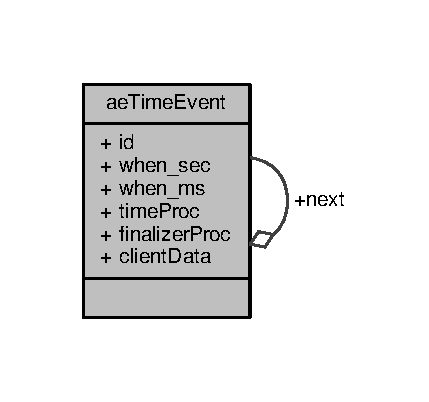
\includegraphics[width=206pt]{structaeTimeEvent__coll__graph}
\end{center}
\end{figure}
\subsection*{Data Fields}
\begin{DoxyCompactItemize}
\item 
\mbox{\Hypertarget{structaeTimeEvent_a24ed4bf76ef40a2c735e9f9cccb45de4}\label{structaeTimeEvent_a24ed4bf76ef40a2c735e9f9cccb45de4}} 
long long {\bfseries id}
\item 
\mbox{\Hypertarget{structaeTimeEvent_a8b8006c68e6af8e1565eda7cbe0ed222}\label{structaeTimeEvent_a8b8006c68e6af8e1565eda7cbe0ed222}} 
long {\bfseries when\+\_\+sec}
\item 
\mbox{\Hypertarget{structaeTimeEvent_aa1c543dc2cfc4d17cf3153c78f373635}\label{structaeTimeEvent_aa1c543dc2cfc4d17cf3153c78f373635}} 
long {\bfseries when\+\_\+ms}
\item 
\mbox{\Hypertarget{structaeTimeEvent_a149629cdd2633c73cfb56e4570bb43ac}\label{structaeTimeEvent_a149629cdd2633c73cfb56e4570bb43ac}} 
ae\+Time\+Proc $\ast$ {\bfseries time\+Proc}
\item 
\mbox{\Hypertarget{structaeTimeEvent_abc682a846c909d98ed1656170bb360f2}\label{structaeTimeEvent_abc682a846c909d98ed1656170bb360f2}} 
ae\+Event\+Finalizer\+Proc $\ast$ {\bfseries finalizer\+Proc}
\item 
\mbox{\Hypertarget{structaeTimeEvent_ad31bed95bafc0baa81fe645f56a11503}\label{structaeTimeEvent_ad31bed95bafc0baa81fe645f56a11503}} 
void $\ast$ {\bfseries client\+Data}
\item 
\mbox{\Hypertarget{structaeTimeEvent_a9721fa6e2866701e2c38f0020beaac60}\label{structaeTimeEvent_a9721fa6e2866701e2c38f0020beaac60}} 
struct \hyperlink{structaeTimeEvent}{ae\+Time\+Event} $\ast$ {\bfseries next}
\end{DoxyCompactItemize}


\subsection{Detailed Description}


Definition at line \hyperlink{ae_8h_source_l00074}{74} of file \hyperlink{ae_8h_source}{ae.\+h}.



\subsection{Field Documentation}
\mbox{\Hypertarget{structaeTimeEvent_ad31bed95bafc0baa81fe645f56a11503}\label{structaeTimeEvent_ad31bed95bafc0baa81fe645f56a11503}} 
\index{ae\+Time\+Event@{ae\+Time\+Event}!client\+Data@{client\+Data}}
\index{client\+Data@{client\+Data}!ae\+Time\+Event@{ae\+Time\+Event}}
\subsubsection{\texorpdfstring{client\+Data}{clientData}}
{\footnotesize\ttfamily void$\ast$ ae\+Time\+Event\+::client\+Data}



Definition at line \hyperlink{ae_8h_source_l00080}{80} of file \hyperlink{ae_8h_source}{ae.\+h}.

\mbox{\Hypertarget{structaeTimeEvent_abc682a846c909d98ed1656170bb360f2}\label{structaeTimeEvent_abc682a846c909d98ed1656170bb360f2}} 
\index{ae\+Time\+Event@{ae\+Time\+Event}!finalizer\+Proc@{finalizer\+Proc}}
\index{finalizer\+Proc@{finalizer\+Proc}!ae\+Time\+Event@{ae\+Time\+Event}}
\subsubsection{\texorpdfstring{finalizer\+Proc}{finalizerProc}}
{\footnotesize\ttfamily ae\+Event\+Finalizer\+Proc$\ast$ ae\+Time\+Event\+::finalizer\+Proc}



Definition at line \hyperlink{ae_8h_source_l00079}{79} of file \hyperlink{ae_8h_source}{ae.\+h}.

\mbox{\Hypertarget{structaeTimeEvent_a24ed4bf76ef40a2c735e9f9cccb45de4}\label{structaeTimeEvent_a24ed4bf76ef40a2c735e9f9cccb45de4}} 
\index{ae\+Time\+Event@{ae\+Time\+Event}!id@{id}}
\index{id@{id}!ae\+Time\+Event@{ae\+Time\+Event}}
\subsubsection{\texorpdfstring{id}{id}}
{\footnotesize\ttfamily long long ae\+Time\+Event\+::id}



Definition at line \hyperlink{ae_8h_source_l00075}{75} of file \hyperlink{ae_8h_source}{ae.\+h}.

\mbox{\Hypertarget{structaeTimeEvent_a9721fa6e2866701e2c38f0020beaac60}\label{structaeTimeEvent_a9721fa6e2866701e2c38f0020beaac60}} 
\index{ae\+Time\+Event@{ae\+Time\+Event}!next@{next}}
\index{next@{next}!ae\+Time\+Event@{ae\+Time\+Event}}
\subsubsection{\texorpdfstring{next}{next}}
{\footnotesize\ttfamily struct \hyperlink{structaeTimeEvent}{ae\+Time\+Event}$\ast$ ae\+Time\+Event\+::next}



Definition at line \hyperlink{ae_8h_source_l00081}{81} of file \hyperlink{ae_8h_source}{ae.\+h}.

\mbox{\Hypertarget{structaeTimeEvent_a149629cdd2633c73cfb56e4570bb43ac}\label{structaeTimeEvent_a149629cdd2633c73cfb56e4570bb43ac}} 
\index{ae\+Time\+Event@{ae\+Time\+Event}!time\+Proc@{time\+Proc}}
\index{time\+Proc@{time\+Proc}!ae\+Time\+Event@{ae\+Time\+Event}}
\subsubsection{\texorpdfstring{time\+Proc}{timeProc}}
{\footnotesize\ttfamily ae\+Time\+Proc$\ast$ ae\+Time\+Event\+::time\+Proc}



Definition at line \hyperlink{ae_8h_source_l00078}{78} of file \hyperlink{ae_8h_source}{ae.\+h}.

\mbox{\Hypertarget{structaeTimeEvent_aa1c543dc2cfc4d17cf3153c78f373635}\label{structaeTimeEvent_aa1c543dc2cfc4d17cf3153c78f373635}} 
\index{ae\+Time\+Event@{ae\+Time\+Event}!when\+\_\+ms@{when\+\_\+ms}}
\index{when\+\_\+ms@{when\+\_\+ms}!ae\+Time\+Event@{ae\+Time\+Event}}
\subsubsection{\texorpdfstring{when\+\_\+ms}{when\_ms}}
{\footnotesize\ttfamily long ae\+Time\+Event\+::when\+\_\+ms}



Definition at line \hyperlink{ae_8h_source_l00077}{77} of file \hyperlink{ae_8h_source}{ae.\+h}.

\mbox{\Hypertarget{structaeTimeEvent_a8b8006c68e6af8e1565eda7cbe0ed222}\label{structaeTimeEvent_a8b8006c68e6af8e1565eda7cbe0ed222}} 
\index{ae\+Time\+Event@{ae\+Time\+Event}!when\+\_\+sec@{when\+\_\+sec}}
\index{when\+\_\+sec@{when\+\_\+sec}!ae\+Time\+Event@{ae\+Time\+Event}}
\subsubsection{\texorpdfstring{when\+\_\+sec}{when\_sec}}
{\footnotesize\ttfamily long ae\+Time\+Event\+::when\+\_\+sec}



Definition at line \hyperlink{ae_8h_source_l00076}{76} of file \hyperlink{ae_8h_source}{ae.\+h}.



The documentation for this struct was generated from the following file\+:\begin{DoxyCompactItemize}
\item 
src/ae.\+h\end{DoxyCompactItemize}

\hypertarget{structaofrwblock}{}\section{aofrwblock Struct Reference}
\label{structaofrwblock}\index{aofrwblock@{aofrwblock}}


Collaboration diagram for aofrwblock\+:\nopagebreak
\begin{figure}[H]
\begin{center}
\leavevmode
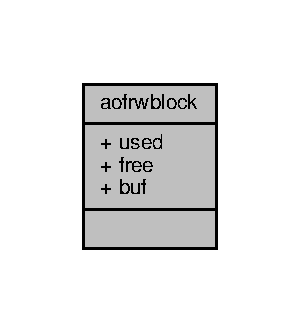
\includegraphics[width=144pt]{structaofrwblock__coll__graph}
\end{center}
\end{figure}
\subsection*{Data Fields}
\begin{DoxyCompactItemize}
\item 
\mbox{\Hypertarget{structaofrwblock_a3169da759f876f081ac1a3b31ac3fae1}\label{structaofrwblock_a3169da759f876f081ac1a3b31ac3fae1}} 
unsigned long {\bfseries used}
\item 
\mbox{\Hypertarget{structaofrwblock_a9eb8333f2c33eb2d1d2cf7e312363bf4}\label{structaofrwblock_a9eb8333f2c33eb2d1d2cf7e312363bf4}} 
unsigned long {\bfseries free}
\item 
\mbox{\Hypertarget{structaofrwblock_a6701e9c90e19caa8d66c46e015bcc314}\label{structaofrwblock_a6701e9c90e19caa8d66c46e015bcc314}} 
char {\bfseries buf} \mbox{[}A\+O\+F\+\_\+\+R\+W\+\_\+\+B\+U\+F\+\_\+\+B\+L\+O\+C\+K\+\_\+\+S\+I\+ZE\mbox{]}
\end{DoxyCompactItemize}


\subsection{Detailed Description}


Definition at line \hyperlink{aof_8c_source_l00062}{62} of file \hyperlink{aof_8c_source}{aof.\+c}.



\subsection{Field Documentation}
\mbox{\Hypertarget{structaofrwblock_a6701e9c90e19caa8d66c46e015bcc314}\label{structaofrwblock_a6701e9c90e19caa8d66c46e015bcc314}} 
\index{aofrwblock@{aofrwblock}!buf@{buf}}
\index{buf@{buf}!aofrwblock@{aofrwblock}}
\subsubsection{\texorpdfstring{buf}{buf}}
{\footnotesize\ttfamily char aofrwblock\+::buf\mbox{[}A\+O\+F\+\_\+\+R\+W\+\_\+\+B\+U\+F\+\_\+\+B\+L\+O\+C\+K\+\_\+\+S\+I\+ZE\mbox{]}}



Definition at line \hyperlink{aof_8c_source_l00064}{64} of file \hyperlink{aof_8c_source}{aof.\+c}.

\mbox{\Hypertarget{structaofrwblock_a9eb8333f2c33eb2d1d2cf7e312363bf4}\label{structaofrwblock_a9eb8333f2c33eb2d1d2cf7e312363bf4}} 
\index{aofrwblock@{aofrwblock}!free@{free}}
\index{free@{free}!aofrwblock@{aofrwblock}}
\subsubsection{\texorpdfstring{free}{free}}
{\footnotesize\ttfamily unsigned long aofrwblock\+::free}



Definition at line \hyperlink{aof_8c_source_l00063}{63} of file \hyperlink{aof_8c_source}{aof.\+c}.

\mbox{\Hypertarget{structaofrwblock_a3169da759f876f081ac1a3b31ac3fae1}\label{structaofrwblock_a3169da759f876f081ac1a3b31ac3fae1}} 
\index{aofrwblock@{aofrwblock}!used@{used}}
\index{used@{used}!aofrwblock@{aofrwblock}}
\subsubsection{\texorpdfstring{used}{used}}
{\footnotesize\ttfamily unsigned long aofrwblock\+::used}



Definition at line \hyperlink{aof_8c_source_l00063}{63} of file \hyperlink{aof_8c_source}{aof.\+c}.



The documentation for this struct was generated from the following file\+:\begin{DoxyCompactItemize}
\item 
src/aof.\+c\end{DoxyCompactItemize}

\hypertarget{structAutoMemEntry}{}\section{Auto\+Mem\+Entry Struct Reference}
\label{structAutoMemEntry}\index{Auto\+Mem\+Entry@{Auto\+Mem\+Entry}}


Collaboration diagram for Auto\+Mem\+Entry\+:\nopagebreak
\begin{figure}[H]
\begin{center}
\leavevmode
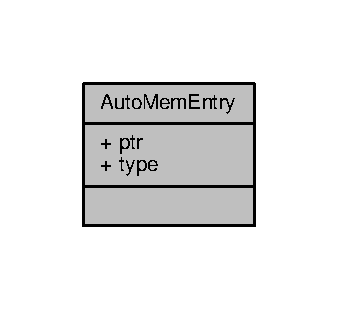
\includegraphics[width=162pt]{structAutoMemEntry__coll__graph}
\end{center}
\end{figure}
\subsection*{Data Fields}
\begin{DoxyCompactItemize}
\item 
\mbox{\Hypertarget{structAutoMemEntry_a900b3ee5c783609e0890be09827e099f}\label{structAutoMemEntry_a900b3ee5c783609e0890be09827e099f}} 
void $\ast$ {\bfseries ptr}
\item 
\mbox{\Hypertarget{structAutoMemEntry_a9df5deaf0ef1229c76c3b63833d71544}\label{structAutoMemEntry_a9df5deaf0ef1229c76c3b63833d71544}} 
int {\bfseries type}
\end{DoxyCompactItemize}


\subsection{Detailed Description}


Definition at line \hyperlink{module_8c_source_l00057}{57} of file \hyperlink{module_8c_source}{module.\+c}.



\subsection{Field Documentation}
\mbox{\Hypertarget{structAutoMemEntry_a900b3ee5c783609e0890be09827e099f}\label{structAutoMemEntry_a900b3ee5c783609e0890be09827e099f}} 
\index{Auto\+Mem\+Entry@{Auto\+Mem\+Entry}!ptr@{ptr}}
\index{ptr@{ptr}!Auto\+Mem\+Entry@{Auto\+Mem\+Entry}}
\subsubsection{\texorpdfstring{ptr}{ptr}}
{\footnotesize\ttfamily void$\ast$ Auto\+Mem\+Entry\+::ptr}



Definition at line \hyperlink{module_8c_source_l00058}{58} of file \hyperlink{module_8c_source}{module.\+c}.

\mbox{\Hypertarget{structAutoMemEntry_a9df5deaf0ef1229c76c3b63833d71544}\label{structAutoMemEntry_a9df5deaf0ef1229c76c3b63833d71544}} 
\index{Auto\+Mem\+Entry@{Auto\+Mem\+Entry}!type@{type}}
\index{type@{type}!Auto\+Mem\+Entry@{Auto\+Mem\+Entry}}
\subsubsection{\texorpdfstring{type}{type}}
{\footnotesize\ttfamily int Auto\+Mem\+Entry\+::type}



Definition at line \hyperlink{module_8c_source_l00059}{59} of file \hyperlink{module_8c_source}{module.\+c}.



The documentation for this struct was generated from the following file\+:\begin{DoxyCompactItemize}
\item 
src/module.\+c\end{DoxyCompactItemize}

\hypertarget{structbio__job}{}\section{bio\+\_\+job Struct Reference}
\label{structbio__job}\index{bio\+\_\+job@{bio\+\_\+job}}


Collaboration diagram for bio\+\_\+job\+:\nopagebreak
\begin{figure}[H]
\begin{center}
\leavevmode
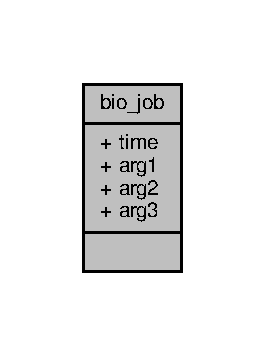
\includegraphics[width=127pt]{structbio__job__coll__graph}
\end{center}
\end{figure}
\subsection*{Data Fields}
\begin{DoxyCompactItemize}
\item 
\mbox{\Hypertarget{structbio__job_a53ba1f8a9fbb41c152e809f9839822f4}\label{structbio__job_a53ba1f8a9fbb41c152e809f9839822f4}} 
time\+\_\+t {\bfseries time}
\item 
\mbox{\Hypertarget{structbio__job_a82f24d16132c2abb05e738c3a84fede2}\label{structbio__job_a82f24d16132c2abb05e738c3a84fede2}} 
void $\ast$ {\bfseries arg1}
\item 
\mbox{\Hypertarget{structbio__job_ad2c73641a7fdc6ecc59a7a653570e7a1}\label{structbio__job_ad2c73641a7fdc6ecc59a7a653570e7a1}} 
void $\ast$ {\bfseries arg2}
\item 
\mbox{\Hypertarget{structbio__job_aff4785b5f684214e4fe1ddeb8b61c63d}\label{structbio__job_aff4785b5f684214e4fe1ddeb8b61c63d}} 
void $\ast$ {\bfseries arg3}
\end{DoxyCompactItemize}


\subsection{Detailed Description}


Definition at line \hyperlink{bio_8c_source_l00079}{79} of file \hyperlink{bio_8c_source}{bio.\+c}.



\subsection{Field Documentation}
\mbox{\Hypertarget{structbio__job_a82f24d16132c2abb05e738c3a84fede2}\label{structbio__job_a82f24d16132c2abb05e738c3a84fede2}} 
\index{bio\+\_\+job@{bio\+\_\+job}!arg1@{arg1}}
\index{arg1@{arg1}!bio\+\_\+job@{bio\+\_\+job}}
\subsubsection{\texorpdfstring{arg1}{arg1}}
{\footnotesize\ttfamily void$\ast$ bio\+\_\+job\+::arg1}



Definition at line \hyperlink{bio_8c_source_l00083}{83} of file \hyperlink{bio_8c_source}{bio.\+c}.

\mbox{\Hypertarget{structbio__job_ad2c73641a7fdc6ecc59a7a653570e7a1}\label{structbio__job_ad2c73641a7fdc6ecc59a7a653570e7a1}} 
\index{bio\+\_\+job@{bio\+\_\+job}!arg2@{arg2}}
\index{arg2@{arg2}!bio\+\_\+job@{bio\+\_\+job}}
\subsubsection{\texorpdfstring{arg2}{arg2}}
{\footnotesize\ttfamily void $\ast$ bio\+\_\+job\+::arg2}



Definition at line \hyperlink{bio_8c_source_l00083}{83} of file \hyperlink{bio_8c_source}{bio.\+c}.

\mbox{\Hypertarget{structbio__job_aff4785b5f684214e4fe1ddeb8b61c63d}\label{structbio__job_aff4785b5f684214e4fe1ddeb8b61c63d}} 
\index{bio\+\_\+job@{bio\+\_\+job}!arg3@{arg3}}
\index{arg3@{arg3}!bio\+\_\+job@{bio\+\_\+job}}
\subsubsection{\texorpdfstring{arg3}{arg3}}
{\footnotesize\ttfamily void $\ast$ bio\+\_\+job\+::arg3}



Definition at line \hyperlink{bio_8c_source_l00083}{83} of file \hyperlink{bio_8c_source}{bio.\+c}.

\mbox{\Hypertarget{structbio__job_a53ba1f8a9fbb41c152e809f9839822f4}\label{structbio__job_a53ba1f8a9fbb41c152e809f9839822f4}} 
\index{bio\+\_\+job@{bio\+\_\+job}!time@{time}}
\index{time@{time}!bio\+\_\+job@{bio\+\_\+job}}
\subsubsection{\texorpdfstring{time}{time}}
{\footnotesize\ttfamily time\+\_\+t bio\+\_\+job\+::time}



Definition at line \hyperlink{bio_8c_source_l00080}{80} of file \hyperlink{bio_8c_source}{bio.\+c}.



The documentation for this struct was generated from the following file\+:\begin{DoxyCompactItemize}
\item 
src/bio.\+c\end{DoxyCompactItemize}

\hypertarget{structbitfieldOp}{}\section{bitfield\+Op Struct Reference}
\label{structbitfieldOp}\index{bitfield\+Op@{bitfield\+Op}}


Collaboration diagram for bitfield\+Op\+:\nopagebreak
\begin{figure}[H]
\begin{center}
\leavevmode
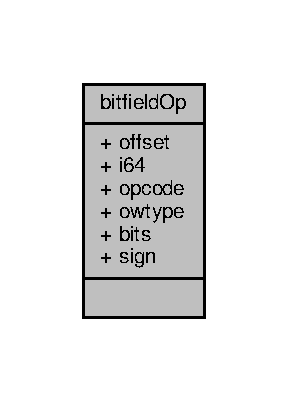
\includegraphics[width=138pt]{structbitfieldOp__coll__graph}
\end{center}
\end{figure}
\subsection*{Data Fields}
\begin{DoxyCompactItemize}
\item 
\mbox{\Hypertarget{structbitfieldOp_aa0548e52311deb47a5bda61b5844f9e5}\label{structbitfieldOp_aa0548e52311deb47a5bda61b5844f9e5}} 
uint64\+\_\+t {\bfseries offset}
\item 
\mbox{\Hypertarget{structbitfieldOp_a4cd6c1beed5d37bed833f4302616bee7}\label{structbitfieldOp_a4cd6c1beed5d37bed833f4302616bee7}} 
int64\+\_\+t {\bfseries i64}
\item 
\mbox{\Hypertarget{structbitfieldOp_a6590f0d17ae13623625a80cc2784b253}\label{structbitfieldOp_a6590f0d17ae13623625a80cc2784b253}} 
int {\bfseries opcode}
\item 
\mbox{\Hypertarget{structbitfieldOp_a4a18ab35d1e0fe98ad934c4e2bb7cb06}\label{structbitfieldOp_a4a18ab35d1e0fe98ad934c4e2bb7cb06}} 
int {\bfseries owtype}
\item 
\mbox{\Hypertarget{structbitfieldOp_a8f086789a4b5e2f2dfa2dc4bfd89d5ed}\label{structbitfieldOp_a8f086789a4b5e2f2dfa2dc4bfd89d5ed}} 
int {\bfseries bits}
\item 
\mbox{\Hypertarget{structbitfieldOp_a469bb961742ba367638b773b4910e1d3}\label{structbitfieldOp_a469bb961742ba367638b773b4910e1d3}} 
int {\bfseries sign}
\end{DoxyCompactItemize}


\subsection{Detailed Description}


Definition at line \hyperlink{bitops_8c_source_l00905}{905} of file \hyperlink{bitops_8c_source}{bitops.\+c}.



\subsection{Field Documentation}
\mbox{\Hypertarget{structbitfieldOp_a8f086789a4b5e2f2dfa2dc4bfd89d5ed}\label{structbitfieldOp_a8f086789a4b5e2f2dfa2dc4bfd89d5ed}} 
\index{bitfield\+Op@{bitfield\+Op}!bits@{bits}}
\index{bits@{bits}!bitfield\+Op@{bitfield\+Op}}
\subsubsection{\texorpdfstring{bits}{bits}}
{\footnotesize\ttfamily int bitfield\+Op\+::bits}



Definition at line \hyperlink{bitops_8c_source_l00910}{910} of file \hyperlink{bitops_8c_source}{bitops.\+c}.

\mbox{\Hypertarget{structbitfieldOp_a4cd6c1beed5d37bed833f4302616bee7}\label{structbitfieldOp_a4cd6c1beed5d37bed833f4302616bee7}} 
\index{bitfield\+Op@{bitfield\+Op}!i64@{i64}}
\index{i64@{i64}!bitfield\+Op@{bitfield\+Op}}
\subsubsection{\texorpdfstring{i64}{i64}}
{\footnotesize\ttfamily int64\+\_\+t bitfield\+Op\+::i64}



Definition at line \hyperlink{bitops_8c_source_l00907}{907} of file \hyperlink{bitops_8c_source}{bitops.\+c}.

\mbox{\Hypertarget{structbitfieldOp_aa0548e52311deb47a5bda61b5844f9e5}\label{structbitfieldOp_aa0548e52311deb47a5bda61b5844f9e5}} 
\index{bitfield\+Op@{bitfield\+Op}!offset@{offset}}
\index{offset@{offset}!bitfield\+Op@{bitfield\+Op}}
\subsubsection{\texorpdfstring{offset}{offset}}
{\footnotesize\ttfamily uint64\+\_\+t bitfield\+Op\+::offset}



Definition at line \hyperlink{bitops_8c_source_l00906}{906} of file \hyperlink{bitops_8c_source}{bitops.\+c}.

\mbox{\Hypertarget{structbitfieldOp_a6590f0d17ae13623625a80cc2784b253}\label{structbitfieldOp_a6590f0d17ae13623625a80cc2784b253}} 
\index{bitfield\+Op@{bitfield\+Op}!opcode@{opcode}}
\index{opcode@{opcode}!bitfield\+Op@{bitfield\+Op}}
\subsubsection{\texorpdfstring{opcode}{opcode}}
{\footnotesize\ttfamily int bitfield\+Op\+::opcode}



Definition at line \hyperlink{bitops_8c_source_l00908}{908} of file \hyperlink{bitops_8c_source}{bitops.\+c}.

\mbox{\Hypertarget{structbitfieldOp_a4a18ab35d1e0fe98ad934c4e2bb7cb06}\label{structbitfieldOp_a4a18ab35d1e0fe98ad934c4e2bb7cb06}} 
\index{bitfield\+Op@{bitfield\+Op}!owtype@{owtype}}
\index{owtype@{owtype}!bitfield\+Op@{bitfield\+Op}}
\subsubsection{\texorpdfstring{owtype}{owtype}}
{\footnotesize\ttfamily int bitfield\+Op\+::owtype}



Definition at line \hyperlink{bitops_8c_source_l00909}{909} of file \hyperlink{bitops_8c_source}{bitops.\+c}.

\mbox{\Hypertarget{structbitfieldOp_a469bb961742ba367638b773b4910e1d3}\label{structbitfieldOp_a469bb961742ba367638b773b4910e1d3}} 
\index{bitfield\+Op@{bitfield\+Op}!sign@{sign}}
\index{sign@{sign}!bitfield\+Op@{bitfield\+Op}}
\subsubsection{\texorpdfstring{sign}{sign}}
{\footnotesize\ttfamily int bitfield\+Op\+::sign}



Definition at line \hyperlink{bitops_8c_source_l00911}{911} of file \hyperlink{bitops_8c_source}{bitops.\+c}.



The documentation for this struct was generated from the following file\+:\begin{DoxyCompactItemize}
\item 
src/bitops.\+c\end{DoxyCompactItemize}

\hypertarget{structblockingState}{}\section{blocking\+State Struct Reference}
\label{structblockingState}\index{blocking\+State@{blocking\+State}}


Collaboration diagram for blocking\+State\+:\nopagebreak
\begin{figure}[H]
\begin{center}
\leavevmode
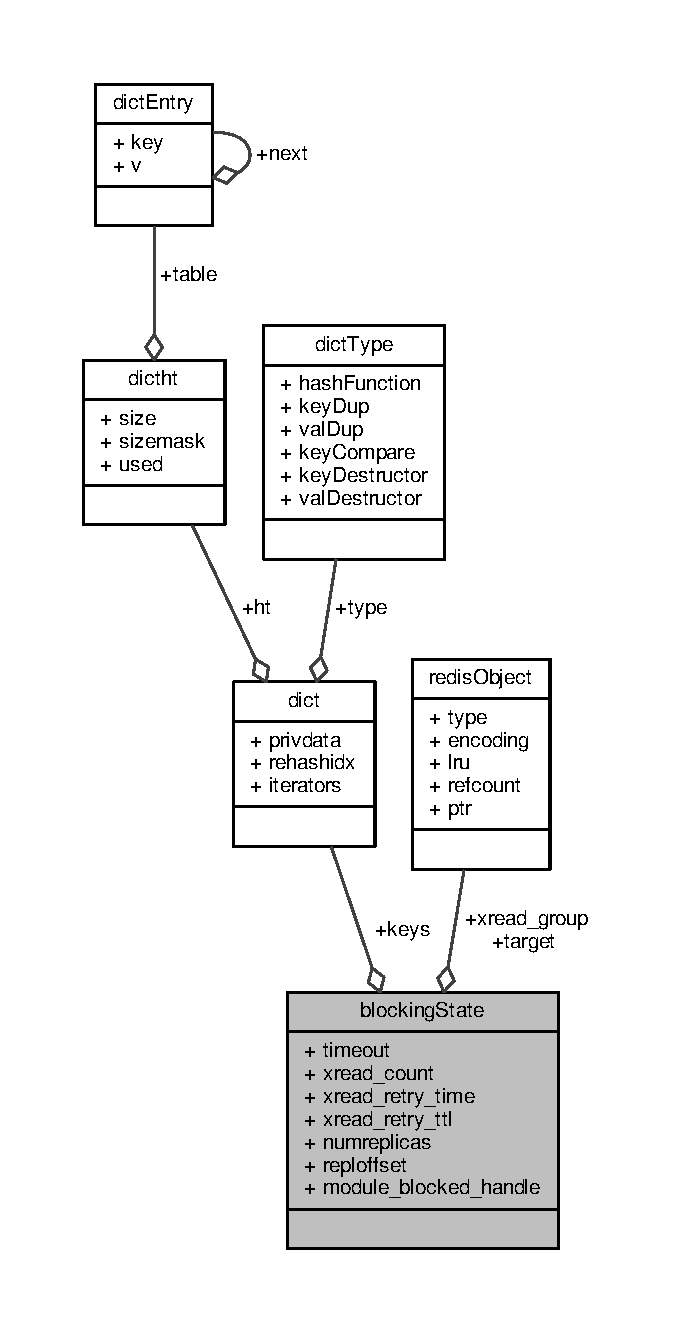
\includegraphics[height=550pt]{structblockingState__coll__graph}
\end{center}
\end{figure}
\subsection*{Data Fields}
\begin{DoxyCompactItemize}
\item 
\mbox{\Hypertarget{structblockingState_a91cba57f48dc0baa84ecea14967aa988}\label{structblockingState_a91cba57f48dc0baa84ecea14967aa988}} 
mstime\+\_\+t {\bfseries timeout}
\item 
\mbox{\Hypertarget{structblockingState_ab76625095616dfdca84124a7f55db2e5}\label{structblockingState_ab76625095616dfdca84124a7f55db2e5}} 
\hyperlink{structdict}{dict} $\ast$ {\bfseries keys}
\item 
\mbox{\Hypertarget{structblockingState_aaa1a98ecc7b021e16e9eb989be9179a0}\label{structblockingState_aaa1a98ecc7b021e16e9eb989be9179a0}} 
\hyperlink{structredisObject}{robj} $\ast$ {\bfseries target}
\item 
\mbox{\Hypertarget{structblockingState_ab5ab9e2de89ee6cb3bb283422f9fcd40}\label{structblockingState_ab5ab9e2de89ee6cb3bb283422f9fcd40}} 
size\+\_\+t {\bfseries xread\+\_\+count}
\item 
\mbox{\Hypertarget{structblockingState_a2989cf7dbfeca2206cacadbff15e76cf}\label{structblockingState_a2989cf7dbfeca2206cacadbff15e76cf}} 
\hyperlink{structredisObject}{robj} $\ast$ {\bfseries xread\+\_\+group}
\item 
\mbox{\Hypertarget{structblockingState_a2039a8b2c8271aacebe826e9bc7d6244}\label{structblockingState_a2039a8b2c8271aacebe826e9bc7d6244}} 
mstime\+\_\+t {\bfseries xread\+\_\+retry\+\_\+time}
\item 
\mbox{\Hypertarget{structblockingState_af9083ecfc8b1f56b60a25afa76e0dd8e}\label{structblockingState_af9083ecfc8b1f56b60a25afa76e0dd8e}} 
mstime\+\_\+t {\bfseries xread\+\_\+retry\+\_\+ttl}
\item 
\mbox{\Hypertarget{structblockingState_a881488caa5361c95b8369973c891ac21}\label{structblockingState_a881488caa5361c95b8369973c891ac21}} 
int {\bfseries numreplicas}
\item 
\mbox{\Hypertarget{structblockingState_a6e19b268054c3ea039a7ecb504010870}\label{structblockingState_a6e19b268054c3ea039a7ecb504010870}} 
long long {\bfseries reploffset}
\item 
\mbox{\Hypertarget{structblockingState_a7b553428255ee211a00c9a9735a84108}\label{structblockingState_a7b553428255ee211a00c9a9735a84108}} 
void $\ast$ {\bfseries module\+\_\+blocked\+\_\+handle}
\end{DoxyCompactItemize}


\subsection{Detailed Description}


Definition at line \hyperlink{server_8h_source_l00642}{642} of file \hyperlink{server_8h_source}{server.\+h}.



\subsection{Field Documentation}
\mbox{\Hypertarget{structblockingState_ab76625095616dfdca84124a7f55db2e5}\label{structblockingState_ab76625095616dfdca84124a7f55db2e5}} 
\index{blocking\+State@{blocking\+State}!keys@{keys}}
\index{keys@{keys}!blocking\+State@{blocking\+State}}
\subsubsection{\texorpdfstring{keys}{keys}}
{\footnotesize\ttfamily \hyperlink{structdict}{dict}$\ast$ blocking\+State\+::keys}



Definition at line \hyperlink{server_8h_source_l00648}{648} of file \hyperlink{server_8h_source}{server.\+h}.

\mbox{\Hypertarget{structblockingState_a7b553428255ee211a00c9a9735a84108}\label{structblockingState_a7b553428255ee211a00c9a9735a84108}} 
\index{blocking\+State@{blocking\+State}!module\+\_\+blocked\+\_\+handle@{module\+\_\+blocked\+\_\+handle}}
\index{module\+\_\+blocked\+\_\+handle@{module\+\_\+blocked\+\_\+handle}!blocking\+State@{blocking\+State}}
\subsubsection{\texorpdfstring{module\+\_\+blocked\+\_\+handle}{module\_blocked\_handle}}
{\footnotesize\ttfamily void$\ast$ blocking\+State\+::module\+\_\+blocked\+\_\+handle}



Definition at line \hyperlink{server_8h_source_l00663}{663} of file \hyperlink{server_8h_source}{server.\+h}.

\mbox{\Hypertarget{structblockingState_a881488caa5361c95b8369973c891ac21}\label{structblockingState_a881488caa5361c95b8369973c891ac21}} 
\index{blocking\+State@{blocking\+State}!numreplicas@{numreplicas}}
\index{numreplicas@{numreplicas}!blocking\+State@{blocking\+State}}
\subsubsection{\texorpdfstring{numreplicas}{numreplicas}}
{\footnotesize\ttfamily int blocking\+State\+::numreplicas}



Definition at line \hyperlink{server_8h_source_l00659}{659} of file \hyperlink{server_8h_source}{server.\+h}.

\mbox{\Hypertarget{structblockingState_a6e19b268054c3ea039a7ecb504010870}\label{structblockingState_a6e19b268054c3ea039a7ecb504010870}} 
\index{blocking\+State@{blocking\+State}!reploffset@{reploffset}}
\index{reploffset@{reploffset}!blocking\+State@{blocking\+State}}
\subsubsection{\texorpdfstring{reploffset}{reploffset}}
{\footnotesize\ttfamily long long blocking\+State\+::reploffset}



Definition at line \hyperlink{server_8h_source_l00660}{660} of file \hyperlink{server_8h_source}{server.\+h}.

\mbox{\Hypertarget{structblockingState_aaa1a98ecc7b021e16e9eb989be9179a0}\label{structblockingState_aaa1a98ecc7b021e16e9eb989be9179a0}} 
\index{blocking\+State@{blocking\+State}!target@{target}}
\index{target@{target}!blocking\+State@{blocking\+State}}
\subsubsection{\texorpdfstring{target}{target}}
{\footnotesize\ttfamily \hyperlink{structredisObject}{robj}$\ast$ blocking\+State\+::target}



Definition at line \hyperlink{server_8h_source_l00650}{650} of file \hyperlink{server_8h_source}{server.\+h}.

\mbox{\Hypertarget{structblockingState_a91cba57f48dc0baa84ecea14967aa988}\label{structblockingState_a91cba57f48dc0baa84ecea14967aa988}} 
\index{blocking\+State@{blocking\+State}!timeout@{timeout}}
\index{timeout@{timeout}!blocking\+State@{blocking\+State}}
\subsubsection{\texorpdfstring{timeout}{timeout}}
{\footnotesize\ttfamily mstime\+\_\+t blocking\+State\+::timeout}



Definition at line \hyperlink{server_8h_source_l00644}{644} of file \hyperlink{server_8h_source}{server.\+h}.

\mbox{\Hypertarget{structblockingState_ab5ab9e2de89ee6cb3bb283422f9fcd40}\label{structblockingState_ab5ab9e2de89ee6cb3bb283422f9fcd40}} 
\index{blocking\+State@{blocking\+State}!xread\+\_\+count@{xread\+\_\+count}}
\index{xread\+\_\+count@{xread\+\_\+count}!blocking\+State@{blocking\+State}}
\subsubsection{\texorpdfstring{xread\+\_\+count}{xread\_count}}
{\footnotesize\ttfamily size\+\_\+t blocking\+State\+::xread\+\_\+count}



Definition at line \hyperlink{server_8h_source_l00654}{654} of file \hyperlink{server_8h_source}{server.\+h}.

\mbox{\Hypertarget{structblockingState_a2989cf7dbfeca2206cacadbff15e76cf}\label{structblockingState_a2989cf7dbfeca2206cacadbff15e76cf}} 
\index{blocking\+State@{blocking\+State}!xread\+\_\+group@{xread\+\_\+group}}
\index{xread\+\_\+group@{xread\+\_\+group}!blocking\+State@{blocking\+State}}
\subsubsection{\texorpdfstring{xread\+\_\+group}{xread\_group}}
{\footnotesize\ttfamily \hyperlink{structredisObject}{robj}$\ast$ blocking\+State\+::xread\+\_\+group}



Definition at line \hyperlink{server_8h_source_l00655}{655} of file \hyperlink{server_8h_source}{server.\+h}.

\mbox{\Hypertarget{structblockingState_a2039a8b2c8271aacebe826e9bc7d6244}\label{structblockingState_a2039a8b2c8271aacebe826e9bc7d6244}} 
\index{blocking\+State@{blocking\+State}!xread\+\_\+retry\+\_\+time@{xread\+\_\+retry\+\_\+time}}
\index{xread\+\_\+retry\+\_\+time@{xread\+\_\+retry\+\_\+time}!blocking\+State@{blocking\+State}}
\subsubsection{\texorpdfstring{xread\+\_\+retry\+\_\+time}{xread\_retry\_time}}
{\footnotesize\ttfamily mstime\+\_\+t blocking\+State\+::xread\+\_\+retry\+\_\+time}



Definition at line \hyperlink{server_8h_source_l00656}{656} of file \hyperlink{server_8h_source}{server.\+h}.

\mbox{\Hypertarget{structblockingState_af9083ecfc8b1f56b60a25afa76e0dd8e}\label{structblockingState_af9083ecfc8b1f56b60a25afa76e0dd8e}} 
\index{blocking\+State@{blocking\+State}!xread\+\_\+retry\+\_\+ttl@{xread\+\_\+retry\+\_\+ttl}}
\index{xread\+\_\+retry\+\_\+ttl@{xread\+\_\+retry\+\_\+ttl}!blocking\+State@{blocking\+State}}
\subsubsection{\texorpdfstring{xread\+\_\+retry\+\_\+ttl}{xread\_retry\_ttl}}
{\footnotesize\ttfamily mstime\+\_\+t blocking\+State\+::xread\+\_\+retry\+\_\+ttl}



Definition at line \hyperlink{server_8h_source_l00656}{656} of file \hyperlink{server_8h_source}{server.\+h}.



The documentation for this struct was generated from the following file\+:\begin{DoxyCompactItemize}
\item 
src/server.\+h\end{DoxyCompactItemize}

\hypertarget{structclient}{}\section{client Struct Reference}
\label{structclient}\index{client@{client}}


Collaboration diagram for client\+:\nopagebreak
\begin{figure}[H]
\begin{center}
\leavevmode
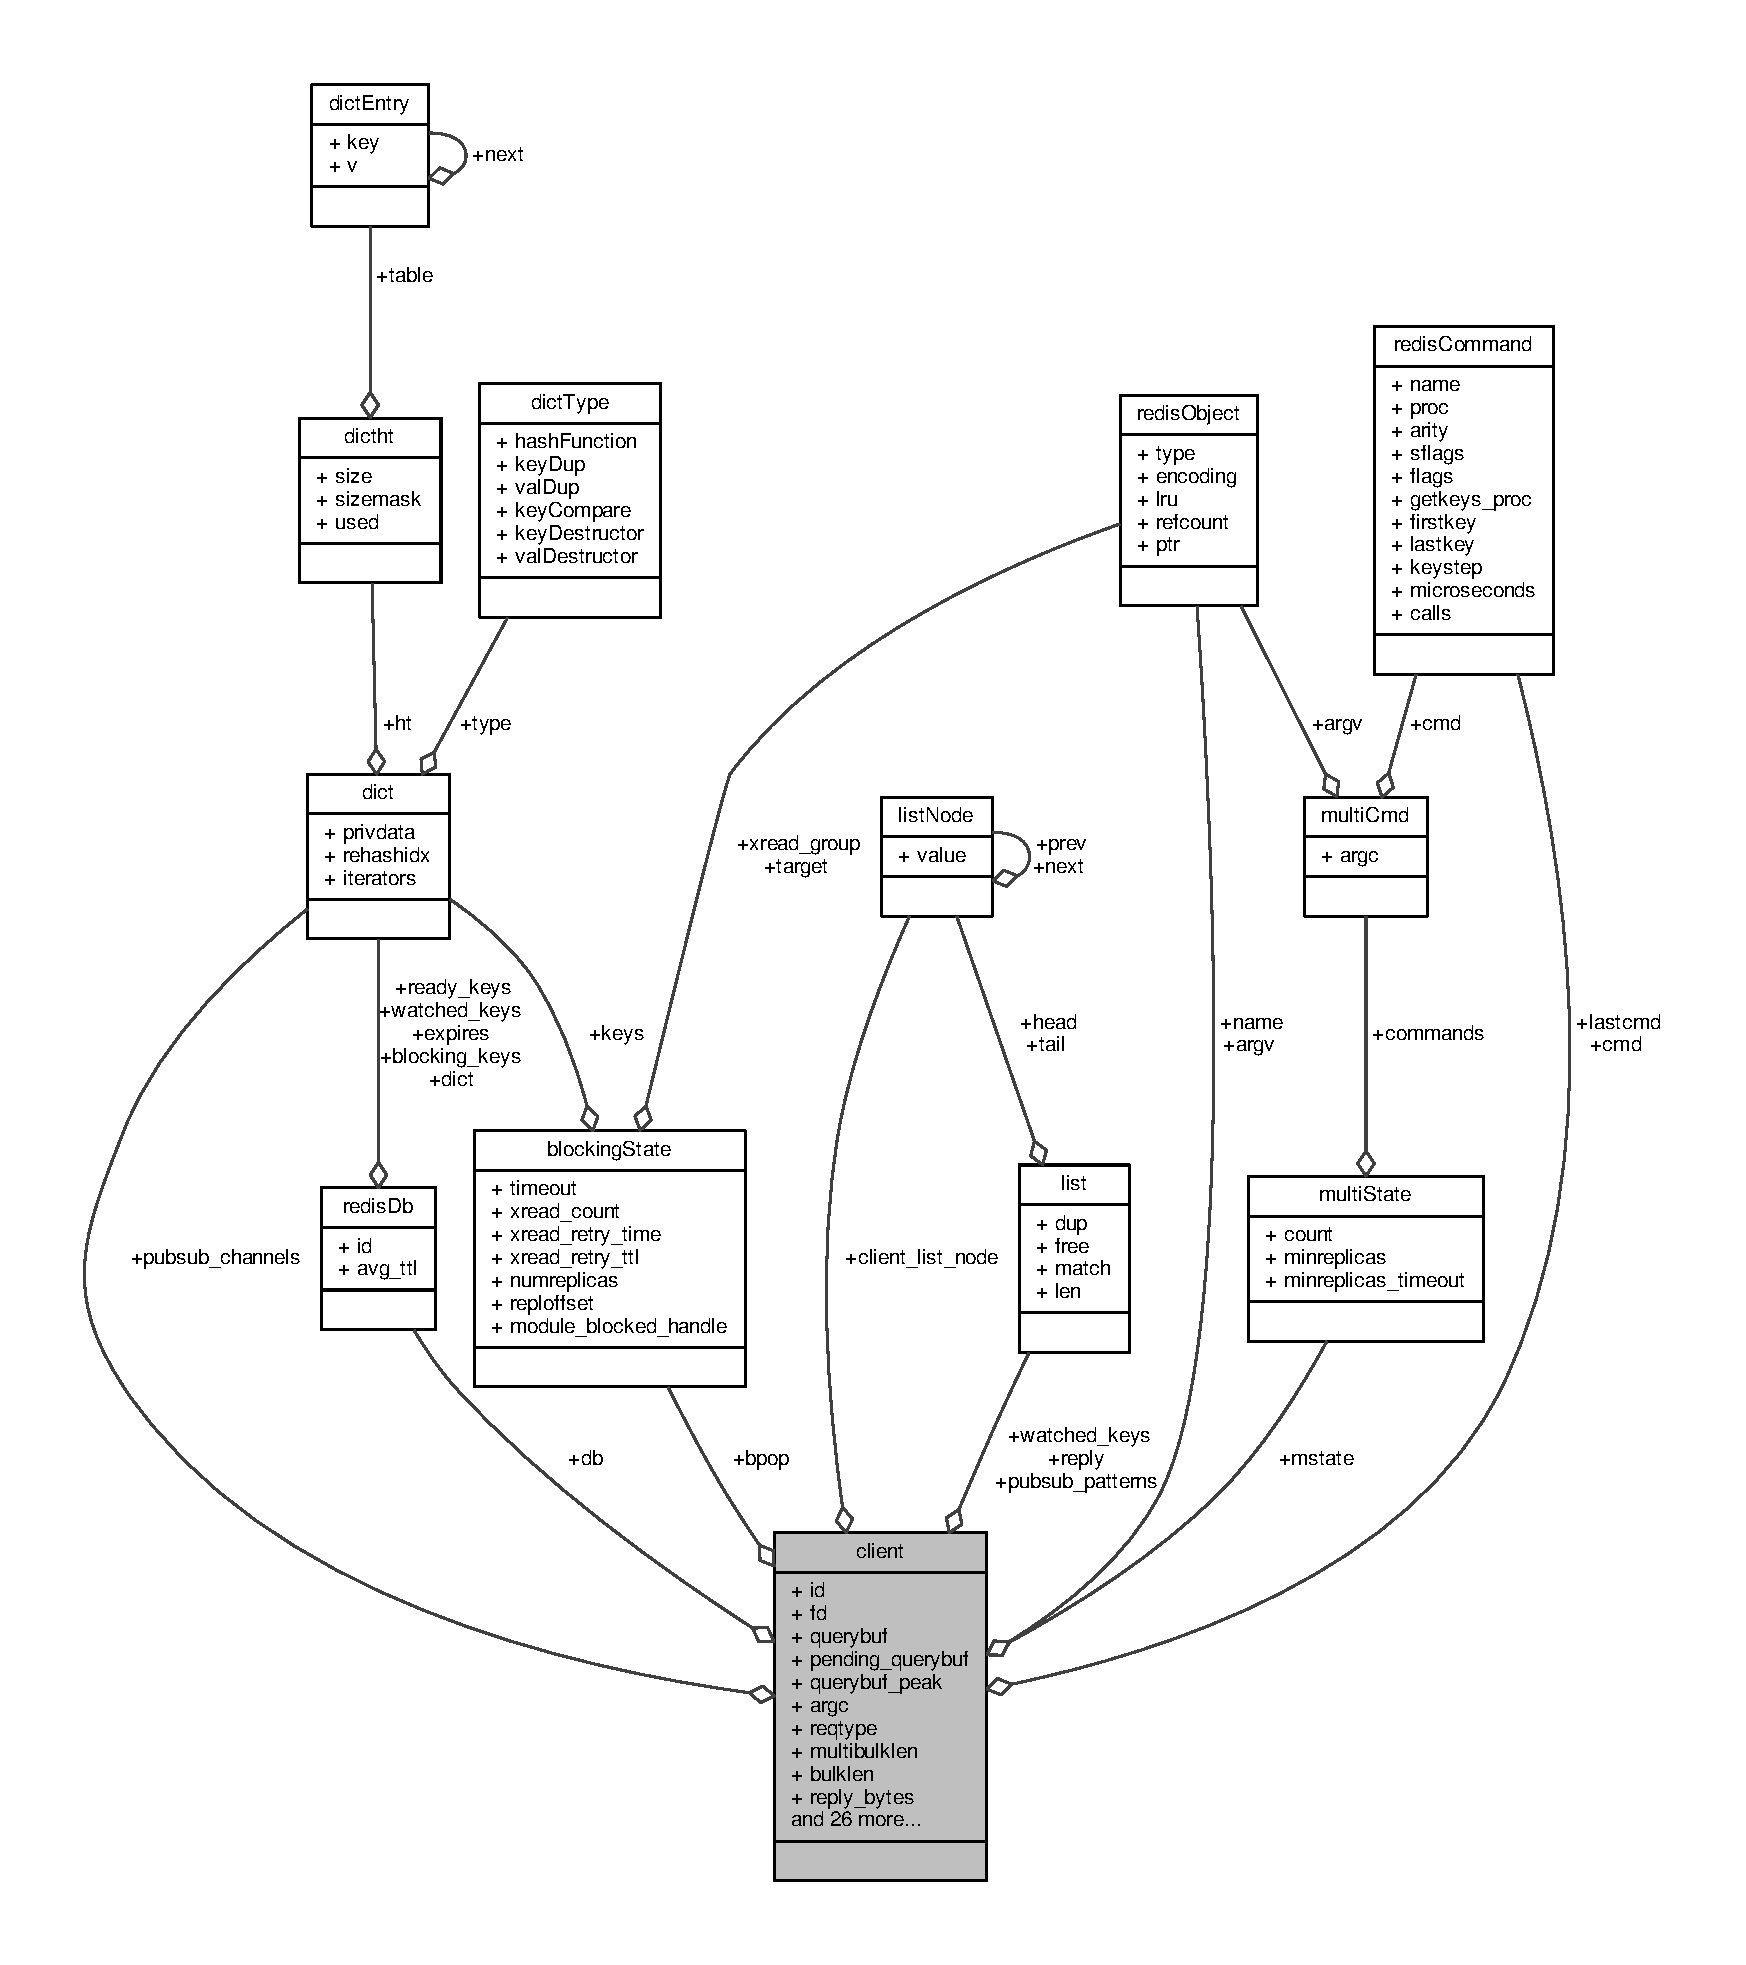
\includegraphics[width=350pt]{structclient__coll__graph}
\end{center}
\end{figure}
\subsection*{Data Fields}
\begin{DoxyCompactItemize}
\item 
\mbox{\Hypertarget{structclient_a3fc8ca078a7db08fb2bd7fd2f3dfcdc6}\label{structclient_a3fc8ca078a7db08fb2bd7fd2f3dfcdc6}} 
uint64\+\_\+t {\bfseries id}
\item 
\mbox{\Hypertarget{structclient_aa9ee781ac58a0d10fa591a570e875473}\label{structclient_aa9ee781ac58a0d10fa591a570e875473}} 
int {\bfseries fd}
\item 
\mbox{\Hypertarget{structclient_a1a3871f1a657729e487cd5d92df32852}\label{structclient_a1a3871f1a657729e487cd5d92df32852}} 
\hyperlink{structredisDb}{redis\+Db} $\ast$ {\bfseries db}
\item 
\mbox{\Hypertarget{structclient_a1568127243d6a623540c7ebe78317a5c}\label{structclient_a1568127243d6a623540c7ebe78317a5c}} 
\hyperlink{structredisObject}{robj} $\ast$ {\bfseries name}
\item 
\mbox{\Hypertarget{structclient_aa95ee1cb708c4fec418c5ad1c838ef64}\label{structclient_aa95ee1cb708c4fec418c5ad1c838ef64}} 
sds {\bfseries querybuf}
\item 
\mbox{\Hypertarget{structclient_a178e18bd0b09afee0d244c1b1e1a46ba}\label{structclient_a178e18bd0b09afee0d244c1b1e1a46ba}} 
sds {\bfseries pending\+\_\+querybuf}
\item 
\mbox{\Hypertarget{structclient_a67800016f1bcbd590adc99028990fdf5}\label{structclient_a67800016f1bcbd590adc99028990fdf5}} 
size\+\_\+t {\bfseries querybuf\+\_\+peak}
\item 
\mbox{\Hypertarget{structclient_a55313c04093c5592241b58a0a25e92f2}\label{structclient_a55313c04093c5592241b58a0a25e92f2}} 
int {\bfseries argc}
\item 
\mbox{\Hypertarget{structclient_ab2db890ba4f68e6438e089b9896328b1}\label{structclient_ab2db890ba4f68e6438e089b9896328b1}} 
\hyperlink{structredisObject}{robj} $\ast$$\ast$ {\bfseries argv}
\item 
\mbox{\Hypertarget{structclient_a072fb7c3464d4f640159169ee4d0a5bc}\label{structclient_a072fb7c3464d4f640159169ee4d0a5bc}} 
struct \hyperlink{structredisCommand}{redis\+Command} $\ast$ {\bfseries cmd}
\item 
\mbox{\Hypertarget{structclient_ac1c9b9f63c1b0ed7f48b6d50111000ae}\label{structclient_ac1c9b9f63c1b0ed7f48b6d50111000ae}} 
struct \hyperlink{structredisCommand}{redis\+Command} $\ast$ {\bfseries lastcmd}
\item 
\mbox{\Hypertarget{structclient_ab2e2a56c21440e3269fa0d6029faac06}\label{structclient_ab2e2a56c21440e3269fa0d6029faac06}} 
int {\bfseries reqtype}
\item 
\mbox{\Hypertarget{structclient_aecec921a67d8d2524164737d4a8f1467}\label{structclient_aecec921a67d8d2524164737d4a8f1467}} 
int {\bfseries multibulklen}
\item 
\mbox{\Hypertarget{structclient_acaa9bcbed32eea1c9fcf60c775b6f498}\label{structclient_acaa9bcbed32eea1c9fcf60c775b6f498}} 
long {\bfseries bulklen}
\item 
\mbox{\Hypertarget{structclient_a76aa9a5fa3b50b5498082076d864a527}\label{structclient_a76aa9a5fa3b50b5498082076d864a527}} 
\hyperlink{structlist}{list} $\ast$ {\bfseries reply}
\item 
\mbox{\Hypertarget{structclient_a86ec8e4ac30913b0abd614b0d7c91742}\label{structclient_a86ec8e4ac30913b0abd614b0d7c91742}} 
unsigned long long {\bfseries reply\+\_\+bytes}
\item 
\mbox{\Hypertarget{structclient_a9a3ef65699c16325e41c3f3416ae62f0}\label{structclient_a9a3ef65699c16325e41c3f3416ae62f0}} 
size\+\_\+t {\bfseries sentlen}
\item 
\mbox{\Hypertarget{structclient_ae2b581131b3efce72bf0607760f7aa06}\label{structclient_ae2b581131b3efce72bf0607760f7aa06}} 
time\+\_\+t {\bfseries ctime}
\item 
\mbox{\Hypertarget{structclient_a5864006ae7f232001e8a8909327c4e86}\label{structclient_a5864006ae7f232001e8a8909327c4e86}} 
time\+\_\+t {\bfseries lastinteraction}
\item 
\mbox{\Hypertarget{structclient_a4fabe12fb4bd7194b041c765ad0f75aa}\label{structclient_a4fabe12fb4bd7194b041c765ad0f75aa}} 
time\+\_\+t {\bfseries obuf\+\_\+soft\+\_\+limit\+\_\+reached\+\_\+time}
\item 
\mbox{\Hypertarget{structclient_a723d126cff0bc975611574cd0004e85a}\label{structclient_a723d126cff0bc975611574cd0004e85a}} 
int {\bfseries flags}
\item 
\mbox{\Hypertarget{structclient_a2c99c8255a1ef51526f26d181b88cdcb}\label{structclient_a2c99c8255a1ef51526f26d181b88cdcb}} 
int {\bfseries authenticated}
\item 
\mbox{\Hypertarget{structclient_a5fca43e8a0ac8735c73ba54af36723ea}\label{structclient_a5fca43e8a0ac8735c73ba54af36723ea}} 
int {\bfseries replstate}
\item 
\mbox{\Hypertarget{structclient_ac372560ae254512b93d940f4c882dc6e}\label{structclient_ac372560ae254512b93d940f4c882dc6e}} 
int {\bfseries repl\+\_\+put\+\_\+online\+\_\+on\+\_\+ack}
\item 
\mbox{\Hypertarget{structclient_af49fbae3663be5fb9cec9abc3e266185}\label{structclient_af49fbae3663be5fb9cec9abc3e266185}} 
int {\bfseries repldbfd}
\item 
\mbox{\Hypertarget{structclient_a63eb4a4b1e825830c07541c922f0e293}\label{structclient_a63eb4a4b1e825830c07541c922f0e293}} 
off\+\_\+t {\bfseries repldboff}
\item 
\mbox{\Hypertarget{structclient_ad81cd83aadbb4e074164fd87f1aeccbd}\label{structclient_ad81cd83aadbb4e074164fd87f1aeccbd}} 
off\+\_\+t {\bfseries repldbsize}
\item 
\mbox{\Hypertarget{structclient_a1ecedfd2fe13d95204235771b03e6b80}\label{structclient_a1ecedfd2fe13d95204235771b03e6b80}} 
sds {\bfseries replpreamble}
\item 
\mbox{\Hypertarget{structclient_adf8f7b46605cf081b77bc45b7174670a}\label{structclient_adf8f7b46605cf081b77bc45b7174670a}} 
long long {\bfseries read\+\_\+reploff}
\item 
\mbox{\Hypertarget{structclient_ab4d6ef175cefe576b0385d103ff2a949}\label{structclient_ab4d6ef175cefe576b0385d103ff2a949}} 
long long {\bfseries reploff}
\item 
\mbox{\Hypertarget{structclient_aed7c294574064dbf283d34be74f62045}\label{structclient_aed7c294574064dbf283d34be74f62045}} 
long long {\bfseries repl\+\_\+ack\+\_\+off}
\item 
\mbox{\Hypertarget{structclient_a3140c1f09c80b09020e200d6489a0677}\label{structclient_a3140c1f09c80b09020e200d6489a0677}} 
long long {\bfseries repl\+\_\+ack\+\_\+time}
\item 
\mbox{\Hypertarget{structclient_ad5a601854272442ac3be11f2080536af}\label{structclient_ad5a601854272442ac3be11f2080536af}} 
long long {\bfseries psync\+\_\+initial\+\_\+offset}
\item 
\mbox{\Hypertarget{structclient_ac7f4047dc671efda5cb77c1708d925ba}\label{structclient_ac7f4047dc671efda5cb77c1708d925ba}} 
char {\bfseries replid} \mbox{[}C\+O\+N\+F\+I\+G\+\_\+\+R\+U\+N\+\_\+\+I\+D\+\_\+\+S\+I\+ZE+1\mbox{]}
\item 
\mbox{\Hypertarget{structclient_a5f127070e4c759e60cdafef415f6eedb}\label{structclient_a5f127070e4c759e60cdafef415f6eedb}} 
int {\bfseries slave\+\_\+listening\+\_\+port}
\item 
\mbox{\Hypertarget{structclient_a1ef9e53d3be4457be63e9c76c8cf147c}\label{structclient_a1ef9e53d3be4457be63e9c76c8cf147c}} 
char {\bfseries slave\+\_\+ip} \mbox{[}N\+E\+T\+\_\+\+I\+P\+\_\+\+S\+T\+R\+\_\+\+L\+EN\mbox{]}
\item 
\mbox{\Hypertarget{structclient_aa9c92fd1ef4933afee5f3b134bc27d43}\label{structclient_aa9c92fd1ef4933afee5f3b134bc27d43}} 
int {\bfseries slave\+\_\+capa}
\item 
\mbox{\Hypertarget{structclient_a275cc795a09bb7b6f24a88f6c37a0f81}\label{structclient_a275cc795a09bb7b6f24a88f6c37a0f81}} 
\hyperlink{structmultiState}{multi\+State} {\bfseries mstate}
\item 
\mbox{\Hypertarget{structclient_a9c1e9d99dd335a598d556a0b940491d3}\label{structclient_a9c1e9d99dd335a598d556a0b940491d3}} 
int {\bfseries btype}
\item 
\mbox{\Hypertarget{structclient_aa2fa244d70ff203607b59b61dc52330e}\label{structclient_aa2fa244d70ff203607b59b61dc52330e}} 
\hyperlink{structblockingState}{blocking\+State} {\bfseries bpop}
\item 
\mbox{\Hypertarget{structclient_afe185dfb331a0a72943f14ab2df60a5d}\label{structclient_afe185dfb331a0a72943f14ab2df60a5d}} 
long long {\bfseries woff}
\item 
\mbox{\Hypertarget{structclient_a6a32880d8716dcdf732846d4b8ac977d}\label{structclient_a6a32880d8716dcdf732846d4b8ac977d}} 
\hyperlink{structlist}{list} $\ast$ {\bfseries watched\+\_\+keys}
\item 
\mbox{\Hypertarget{structclient_a387de498270f2a643eaf671fd058203b}\label{structclient_a387de498270f2a643eaf671fd058203b}} 
\hyperlink{structdict}{dict} $\ast$ {\bfseries pubsub\+\_\+channels}
\item 
\mbox{\Hypertarget{structclient_a811d6395007358fcf349a4d57bda2715}\label{structclient_a811d6395007358fcf349a4d57bda2715}} 
\hyperlink{structlist}{list} $\ast$ {\bfseries pubsub\+\_\+patterns}
\item 
\mbox{\Hypertarget{structclient_a6edab5d6742ec650d28f2952d46953bb}\label{structclient_a6edab5d6742ec650d28f2952d46953bb}} 
sds {\bfseries peerid}
\item 
\mbox{\Hypertarget{structclient_a3bf7cb0753f83fba41bc06368914d288}\label{structclient_a3bf7cb0753f83fba41bc06368914d288}} 
\hyperlink{structlistNode}{list\+Node} $\ast$ {\bfseries client\+\_\+list\+\_\+node}
\item 
\mbox{\Hypertarget{structclient_a43d6f0929a1c0f187c06b5f777c8f1b7}\label{structclient_a43d6f0929a1c0f187c06b5f777c8f1b7}} 
int {\bfseries bufpos}
\item 
\mbox{\Hypertarget{structclient_a3566e777060a8cdb289a0f585bea72cd}\label{structclient_a3566e777060a8cdb289a0f585bea72cd}} 
char {\bfseries buf} \mbox{[}P\+R\+O\+T\+O\+\_\+\+R\+E\+P\+L\+Y\+\_\+\+C\+H\+U\+N\+K\+\_\+\+B\+Y\+T\+ES\mbox{]}
\end{DoxyCompactItemize}


\subsection{Detailed Description}


Definition at line \hyperlink{server_8h_source_l00686}{686} of file \hyperlink{server_8h_source}{server.\+h}.



\subsection{Field Documentation}
\mbox{\Hypertarget{structclient_a55313c04093c5592241b58a0a25e92f2}\label{structclient_a55313c04093c5592241b58a0a25e92f2}} 
\index{client@{client}!argc@{argc}}
\index{argc@{argc}!client@{client}}
\subsubsection{\texorpdfstring{argc}{argc}}
{\footnotesize\ttfamily int client\+::argc}



Definition at line \hyperlink{server_8h_source_l00696}{696} of file \hyperlink{server_8h_source}{server.\+h}.

\mbox{\Hypertarget{structclient_ab2db890ba4f68e6438e089b9896328b1}\label{structclient_ab2db890ba4f68e6438e089b9896328b1}} 
\index{client@{client}!argv@{argv}}
\index{argv@{argv}!client@{client}}
\subsubsection{\texorpdfstring{argv}{argv}}
{\footnotesize\ttfamily \hyperlink{structredisObject}{robj}$\ast$$\ast$ client\+::argv}



Definition at line \hyperlink{server_8h_source_l00697}{697} of file \hyperlink{server_8h_source}{server.\+h}.

\mbox{\Hypertarget{structclient_a2c99c8255a1ef51526f26d181b88cdcb}\label{structclient_a2c99c8255a1ef51526f26d181b88cdcb}} 
\index{client@{client}!authenticated@{authenticated}}
\index{authenticated@{authenticated}!client@{client}}
\subsubsection{\texorpdfstring{authenticated}{authenticated}}
{\footnotesize\ttfamily int client\+::authenticated}



Definition at line \hyperlink{server_8h_source_l00710}{710} of file \hyperlink{server_8h_source}{server.\+h}.

\mbox{\Hypertarget{structclient_aa2fa244d70ff203607b59b61dc52330e}\label{structclient_aa2fa244d70ff203607b59b61dc52330e}} 
\index{client@{client}!bpop@{bpop}}
\index{bpop@{bpop}!client@{client}}
\subsubsection{\texorpdfstring{bpop}{bpop}}
{\footnotesize\ttfamily \hyperlink{structblockingState}{blocking\+State} client\+::bpop}



Definition at line \hyperlink{server_8h_source_l00730}{730} of file \hyperlink{server_8h_source}{server.\+h}.

\mbox{\Hypertarget{structclient_a9c1e9d99dd335a598d556a0b940491d3}\label{structclient_a9c1e9d99dd335a598d556a0b940491d3}} 
\index{client@{client}!btype@{btype}}
\index{btype@{btype}!client@{client}}
\subsubsection{\texorpdfstring{btype}{btype}}
{\footnotesize\ttfamily int client\+::btype}



Definition at line \hyperlink{server_8h_source_l00729}{729} of file \hyperlink{server_8h_source}{server.\+h}.

\mbox{\Hypertarget{structclient_a3566e777060a8cdb289a0f585bea72cd}\label{structclient_a3566e777060a8cdb289a0f585bea72cd}} 
\index{client@{client}!buf@{buf}}
\index{buf@{buf}!client@{client}}
\subsubsection{\texorpdfstring{buf}{buf}}
{\footnotesize\ttfamily char client\+::buf\mbox{[}P\+R\+O\+T\+O\+\_\+\+R\+E\+P\+L\+Y\+\_\+\+C\+H\+U\+N\+K\+\_\+\+B\+Y\+T\+ES\mbox{]}}



Definition at line \hyperlink{server_8h_source_l00740}{740} of file \hyperlink{server_8h_source}{server.\+h}.

\mbox{\Hypertarget{structclient_a43d6f0929a1c0f187c06b5f777c8f1b7}\label{structclient_a43d6f0929a1c0f187c06b5f777c8f1b7}} 
\index{client@{client}!bufpos@{bufpos}}
\index{bufpos@{bufpos}!client@{client}}
\subsubsection{\texorpdfstring{bufpos}{bufpos}}
{\footnotesize\ttfamily int client\+::bufpos}



Definition at line \hyperlink{server_8h_source_l00739}{739} of file \hyperlink{server_8h_source}{server.\+h}.

\mbox{\Hypertarget{structclient_acaa9bcbed32eea1c9fcf60c775b6f498}\label{structclient_acaa9bcbed32eea1c9fcf60c775b6f498}} 
\index{client@{client}!bulklen@{bulklen}}
\index{bulklen@{bulklen}!client@{client}}
\subsubsection{\texorpdfstring{bulklen}{bulklen}}
{\footnotesize\ttfamily long client\+::bulklen}



Definition at line \hyperlink{server_8h_source_l00701}{701} of file \hyperlink{server_8h_source}{server.\+h}.

\mbox{\Hypertarget{structclient_a3bf7cb0753f83fba41bc06368914d288}\label{structclient_a3bf7cb0753f83fba41bc06368914d288}} 
\index{client@{client}!client\+\_\+list\+\_\+node@{client\+\_\+list\+\_\+node}}
\index{client\+\_\+list\+\_\+node@{client\+\_\+list\+\_\+node}!client@{client}}
\subsubsection{\texorpdfstring{client\+\_\+list\+\_\+node}{client\_list\_node}}
{\footnotesize\ttfamily \hyperlink{structlistNode}{list\+Node}$\ast$ client\+::client\+\_\+list\+\_\+node}



Definition at line \hyperlink{server_8h_source_l00736}{736} of file \hyperlink{server_8h_source}{server.\+h}.

\mbox{\Hypertarget{structclient_a072fb7c3464d4f640159169ee4d0a5bc}\label{structclient_a072fb7c3464d4f640159169ee4d0a5bc}} 
\index{client@{client}!cmd@{cmd}}
\index{cmd@{cmd}!client@{client}}
\subsubsection{\texorpdfstring{cmd}{cmd}}
{\footnotesize\ttfamily struct \hyperlink{structredisCommand}{redis\+Command}$\ast$ client\+::cmd}



Definition at line \hyperlink{server_8h_source_l00698}{698} of file \hyperlink{server_8h_source}{server.\+h}.

\mbox{\Hypertarget{structclient_ae2b581131b3efce72bf0607760f7aa06}\label{structclient_ae2b581131b3efce72bf0607760f7aa06}} 
\index{client@{client}!ctime@{ctime}}
\index{ctime@{ctime}!client@{client}}
\subsubsection{\texorpdfstring{ctime}{ctime}}
{\footnotesize\ttfamily time\+\_\+t client\+::ctime}



Definition at line \hyperlink{server_8h_source_l00706}{706} of file \hyperlink{server_8h_source}{server.\+h}.

\mbox{\Hypertarget{structclient_a1a3871f1a657729e487cd5d92df32852}\label{structclient_a1a3871f1a657729e487cd5d92df32852}} 
\index{client@{client}!db@{db}}
\index{db@{db}!client@{client}}
\subsubsection{\texorpdfstring{db}{db}}
{\footnotesize\ttfamily \hyperlink{structredisDb}{redis\+Db}$\ast$ client\+::db}



Definition at line \hyperlink{server_8h_source_l00689}{689} of file \hyperlink{server_8h_source}{server.\+h}.

\mbox{\Hypertarget{structclient_aa9ee781ac58a0d10fa591a570e875473}\label{structclient_aa9ee781ac58a0d10fa591a570e875473}} 
\index{client@{client}!fd@{fd}}
\index{fd@{fd}!client@{client}}
\subsubsection{\texorpdfstring{fd}{fd}}
{\footnotesize\ttfamily int client\+::fd}



Definition at line \hyperlink{server_8h_source_l00688}{688} of file \hyperlink{server_8h_source}{server.\+h}.

\mbox{\Hypertarget{structclient_a723d126cff0bc975611574cd0004e85a}\label{structclient_a723d126cff0bc975611574cd0004e85a}} 
\index{client@{client}!flags@{flags}}
\index{flags@{flags}!client@{client}}
\subsubsection{\texorpdfstring{flags}{flags}}
{\footnotesize\ttfamily int client\+::flags}



Definition at line \hyperlink{server_8h_source_l00709}{709} of file \hyperlink{server_8h_source}{server.\+h}.

\mbox{\Hypertarget{structclient_a3fc8ca078a7db08fb2bd7fd2f3dfcdc6}\label{structclient_a3fc8ca078a7db08fb2bd7fd2f3dfcdc6}} 
\index{client@{client}!id@{id}}
\index{id@{id}!client@{client}}
\subsubsection{\texorpdfstring{id}{id}}
{\footnotesize\ttfamily uint64\+\_\+t client\+::id}



Definition at line \hyperlink{server_8h_source_l00687}{687} of file \hyperlink{server_8h_source}{server.\+h}.

\mbox{\Hypertarget{structclient_ac1c9b9f63c1b0ed7f48b6d50111000ae}\label{structclient_ac1c9b9f63c1b0ed7f48b6d50111000ae}} 
\index{client@{client}!lastcmd@{lastcmd}}
\index{lastcmd@{lastcmd}!client@{client}}
\subsubsection{\texorpdfstring{lastcmd}{lastcmd}}
{\footnotesize\ttfamily struct \hyperlink{structredisCommand}{redis\+Command} $\ast$ client\+::lastcmd}



Definition at line \hyperlink{server_8h_source_l00698}{698} of file \hyperlink{server_8h_source}{server.\+h}.

\mbox{\Hypertarget{structclient_a5864006ae7f232001e8a8909327c4e86}\label{structclient_a5864006ae7f232001e8a8909327c4e86}} 
\index{client@{client}!lastinteraction@{lastinteraction}}
\index{lastinteraction@{lastinteraction}!client@{client}}
\subsubsection{\texorpdfstring{lastinteraction}{lastinteraction}}
{\footnotesize\ttfamily time\+\_\+t client\+::lastinteraction}



Definition at line \hyperlink{server_8h_source_l00707}{707} of file \hyperlink{server_8h_source}{server.\+h}.

\mbox{\Hypertarget{structclient_a275cc795a09bb7b6f24a88f6c37a0f81}\label{structclient_a275cc795a09bb7b6f24a88f6c37a0f81}} 
\index{client@{client}!mstate@{mstate}}
\index{mstate@{mstate}!client@{client}}
\subsubsection{\texorpdfstring{mstate}{mstate}}
{\footnotesize\ttfamily \hyperlink{structmultiState}{multi\+State} client\+::mstate}



Definition at line \hyperlink{server_8h_source_l00728}{728} of file \hyperlink{server_8h_source}{server.\+h}.

\mbox{\Hypertarget{structclient_aecec921a67d8d2524164737d4a8f1467}\label{structclient_aecec921a67d8d2524164737d4a8f1467}} 
\index{client@{client}!multibulklen@{multibulklen}}
\index{multibulklen@{multibulklen}!client@{client}}
\subsubsection{\texorpdfstring{multibulklen}{multibulklen}}
{\footnotesize\ttfamily int client\+::multibulklen}



Definition at line \hyperlink{server_8h_source_l00700}{700} of file \hyperlink{server_8h_source}{server.\+h}.

\mbox{\Hypertarget{structclient_a1568127243d6a623540c7ebe78317a5c}\label{structclient_a1568127243d6a623540c7ebe78317a5c}} 
\index{client@{client}!name@{name}}
\index{name@{name}!client@{client}}
\subsubsection{\texorpdfstring{name}{name}}
{\footnotesize\ttfamily \hyperlink{structredisObject}{robj}$\ast$ client\+::name}



Definition at line \hyperlink{server_8h_source_l00690}{690} of file \hyperlink{server_8h_source}{server.\+h}.

\mbox{\Hypertarget{structclient_a4fabe12fb4bd7194b041c765ad0f75aa}\label{structclient_a4fabe12fb4bd7194b041c765ad0f75aa}} 
\index{client@{client}!obuf\+\_\+soft\+\_\+limit\+\_\+reached\+\_\+time@{obuf\+\_\+soft\+\_\+limit\+\_\+reached\+\_\+time}}
\index{obuf\+\_\+soft\+\_\+limit\+\_\+reached\+\_\+time@{obuf\+\_\+soft\+\_\+limit\+\_\+reached\+\_\+time}!client@{client}}
\subsubsection{\texorpdfstring{obuf\+\_\+soft\+\_\+limit\+\_\+reached\+\_\+time}{obuf\_soft\_limit\_reached\_time}}
{\footnotesize\ttfamily time\+\_\+t client\+::obuf\+\_\+soft\+\_\+limit\+\_\+reached\+\_\+time}



Definition at line \hyperlink{server_8h_source_l00708}{708} of file \hyperlink{server_8h_source}{server.\+h}.

\mbox{\Hypertarget{structclient_a6edab5d6742ec650d28f2952d46953bb}\label{structclient_a6edab5d6742ec650d28f2952d46953bb}} 
\index{client@{client}!peerid@{peerid}}
\index{peerid@{peerid}!client@{client}}
\subsubsection{\texorpdfstring{peerid}{peerid}}
{\footnotesize\ttfamily sds client\+::peerid}



Definition at line \hyperlink{server_8h_source_l00735}{735} of file \hyperlink{server_8h_source}{server.\+h}.

\mbox{\Hypertarget{structclient_a178e18bd0b09afee0d244c1b1e1a46ba}\label{structclient_a178e18bd0b09afee0d244c1b1e1a46ba}} 
\index{client@{client}!pending\+\_\+querybuf@{pending\+\_\+querybuf}}
\index{pending\+\_\+querybuf@{pending\+\_\+querybuf}!client@{client}}
\subsubsection{\texorpdfstring{pending\+\_\+querybuf}{pending\_querybuf}}
{\footnotesize\ttfamily sds client\+::pending\+\_\+querybuf}



Definition at line \hyperlink{server_8h_source_l00692}{692} of file \hyperlink{server_8h_source}{server.\+h}.

\mbox{\Hypertarget{structclient_ad5a601854272442ac3be11f2080536af}\label{structclient_ad5a601854272442ac3be11f2080536af}} 
\index{client@{client}!psync\+\_\+initial\+\_\+offset@{psync\+\_\+initial\+\_\+offset}}
\index{psync\+\_\+initial\+\_\+offset@{psync\+\_\+initial\+\_\+offset}!client@{client}}
\subsubsection{\texorpdfstring{psync\+\_\+initial\+\_\+offset}{psync\_initial\_offset}}
{\footnotesize\ttfamily long long client\+::psync\+\_\+initial\+\_\+offset}



Definition at line \hyperlink{server_8h_source_l00721}{721} of file \hyperlink{server_8h_source}{server.\+h}.

\mbox{\Hypertarget{structclient_a387de498270f2a643eaf671fd058203b}\label{structclient_a387de498270f2a643eaf671fd058203b}} 
\index{client@{client}!pubsub\+\_\+channels@{pubsub\+\_\+channels}}
\index{pubsub\+\_\+channels@{pubsub\+\_\+channels}!client@{client}}
\subsubsection{\texorpdfstring{pubsub\+\_\+channels}{pubsub\_channels}}
{\footnotesize\ttfamily \hyperlink{structdict}{dict}$\ast$ client\+::pubsub\+\_\+channels}



Definition at line \hyperlink{server_8h_source_l00733}{733} of file \hyperlink{server_8h_source}{server.\+h}.

\mbox{\Hypertarget{structclient_a811d6395007358fcf349a4d57bda2715}\label{structclient_a811d6395007358fcf349a4d57bda2715}} 
\index{client@{client}!pubsub\+\_\+patterns@{pubsub\+\_\+patterns}}
\index{pubsub\+\_\+patterns@{pubsub\+\_\+patterns}!client@{client}}
\subsubsection{\texorpdfstring{pubsub\+\_\+patterns}{pubsub\_patterns}}
{\footnotesize\ttfamily \hyperlink{structlist}{list}$\ast$ client\+::pubsub\+\_\+patterns}



Definition at line \hyperlink{server_8h_source_l00734}{734} of file \hyperlink{server_8h_source}{server.\+h}.

\mbox{\Hypertarget{structclient_aa95ee1cb708c4fec418c5ad1c838ef64}\label{structclient_aa95ee1cb708c4fec418c5ad1c838ef64}} 
\index{client@{client}!querybuf@{querybuf}}
\index{querybuf@{querybuf}!client@{client}}
\subsubsection{\texorpdfstring{querybuf}{querybuf}}
{\footnotesize\ttfamily sds client\+::querybuf}



Definition at line \hyperlink{server_8h_source_l00691}{691} of file \hyperlink{server_8h_source}{server.\+h}.

\mbox{\Hypertarget{structclient_a67800016f1bcbd590adc99028990fdf5}\label{structclient_a67800016f1bcbd590adc99028990fdf5}} 
\index{client@{client}!querybuf\+\_\+peak@{querybuf\+\_\+peak}}
\index{querybuf\+\_\+peak@{querybuf\+\_\+peak}!client@{client}}
\subsubsection{\texorpdfstring{querybuf\+\_\+peak}{querybuf\_peak}}
{\footnotesize\ttfamily size\+\_\+t client\+::querybuf\+\_\+peak}



Definition at line \hyperlink{server_8h_source_l00695}{695} of file \hyperlink{server_8h_source}{server.\+h}.

\mbox{\Hypertarget{structclient_adf8f7b46605cf081b77bc45b7174670a}\label{structclient_adf8f7b46605cf081b77bc45b7174670a}} 
\index{client@{client}!read\+\_\+reploff@{read\+\_\+reploff}}
\index{read\+\_\+reploff@{read\+\_\+reploff}!client@{client}}
\subsubsection{\texorpdfstring{read\+\_\+reploff}{read\_reploff}}
{\footnotesize\ttfamily long long client\+::read\+\_\+reploff}



Definition at line \hyperlink{server_8h_source_l00717}{717} of file \hyperlink{server_8h_source}{server.\+h}.

\mbox{\Hypertarget{structclient_aed7c294574064dbf283d34be74f62045}\label{structclient_aed7c294574064dbf283d34be74f62045}} 
\index{client@{client}!repl\+\_\+ack\+\_\+off@{repl\+\_\+ack\+\_\+off}}
\index{repl\+\_\+ack\+\_\+off@{repl\+\_\+ack\+\_\+off}!client@{client}}
\subsubsection{\texorpdfstring{repl\+\_\+ack\+\_\+off}{repl\_ack\_off}}
{\footnotesize\ttfamily long long client\+::repl\+\_\+ack\+\_\+off}



Definition at line \hyperlink{server_8h_source_l00719}{719} of file \hyperlink{server_8h_source}{server.\+h}.

\mbox{\Hypertarget{structclient_a3140c1f09c80b09020e200d6489a0677}\label{structclient_a3140c1f09c80b09020e200d6489a0677}} 
\index{client@{client}!repl\+\_\+ack\+\_\+time@{repl\+\_\+ack\+\_\+time}}
\index{repl\+\_\+ack\+\_\+time@{repl\+\_\+ack\+\_\+time}!client@{client}}
\subsubsection{\texorpdfstring{repl\+\_\+ack\+\_\+time}{repl\_ack\_time}}
{\footnotesize\ttfamily long long client\+::repl\+\_\+ack\+\_\+time}



Definition at line \hyperlink{server_8h_source_l00720}{720} of file \hyperlink{server_8h_source}{server.\+h}.

\mbox{\Hypertarget{structclient_ac372560ae254512b93d940f4c882dc6e}\label{structclient_ac372560ae254512b93d940f4c882dc6e}} 
\index{client@{client}!repl\+\_\+put\+\_\+online\+\_\+on\+\_\+ack@{repl\+\_\+put\+\_\+online\+\_\+on\+\_\+ack}}
\index{repl\+\_\+put\+\_\+online\+\_\+on\+\_\+ack@{repl\+\_\+put\+\_\+online\+\_\+on\+\_\+ack}!client@{client}}
\subsubsection{\texorpdfstring{repl\+\_\+put\+\_\+online\+\_\+on\+\_\+ack}{repl\_put\_online\_on\_ack}}
{\footnotesize\ttfamily int client\+::repl\+\_\+put\+\_\+online\+\_\+on\+\_\+ack}



Definition at line \hyperlink{server_8h_source_l00712}{712} of file \hyperlink{server_8h_source}{server.\+h}.

\mbox{\Hypertarget{structclient_af49fbae3663be5fb9cec9abc3e266185}\label{structclient_af49fbae3663be5fb9cec9abc3e266185}} 
\index{client@{client}!repldbfd@{repldbfd}}
\index{repldbfd@{repldbfd}!client@{client}}
\subsubsection{\texorpdfstring{repldbfd}{repldbfd}}
{\footnotesize\ttfamily int client\+::repldbfd}



Definition at line \hyperlink{server_8h_source_l00713}{713} of file \hyperlink{server_8h_source}{server.\+h}.

\mbox{\Hypertarget{structclient_a63eb4a4b1e825830c07541c922f0e293}\label{structclient_a63eb4a4b1e825830c07541c922f0e293}} 
\index{client@{client}!repldboff@{repldboff}}
\index{repldboff@{repldboff}!client@{client}}
\subsubsection{\texorpdfstring{repldboff}{repldboff}}
{\footnotesize\ttfamily off\+\_\+t client\+::repldboff}



Definition at line \hyperlink{server_8h_source_l00714}{714} of file \hyperlink{server_8h_source}{server.\+h}.

\mbox{\Hypertarget{structclient_ad81cd83aadbb4e074164fd87f1aeccbd}\label{structclient_ad81cd83aadbb4e074164fd87f1aeccbd}} 
\index{client@{client}!repldbsize@{repldbsize}}
\index{repldbsize@{repldbsize}!client@{client}}
\subsubsection{\texorpdfstring{repldbsize}{repldbsize}}
{\footnotesize\ttfamily off\+\_\+t client\+::repldbsize}



Definition at line \hyperlink{server_8h_source_l00715}{715} of file \hyperlink{server_8h_source}{server.\+h}.

\mbox{\Hypertarget{structclient_ac7f4047dc671efda5cb77c1708d925ba}\label{structclient_ac7f4047dc671efda5cb77c1708d925ba}} 
\index{client@{client}!replid@{replid}}
\index{replid@{replid}!client@{client}}
\subsubsection{\texorpdfstring{replid}{replid}}
{\footnotesize\ttfamily char client\+::replid\mbox{[}C\+O\+N\+F\+I\+G\+\_\+\+R\+U\+N\+\_\+\+I\+D\+\_\+\+S\+I\+ZE+1\mbox{]}}



Definition at line \hyperlink{server_8h_source_l00724}{724} of file \hyperlink{server_8h_source}{server.\+h}.

\mbox{\Hypertarget{structclient_ab4d6ef175cefe576b0385d103ff2a949}\label{structclient_ab4d6ef175cefe576b0385d103ff2a949}} 
\index{client@{client}!reploff@{reploff}}
\index{reploff@{reploff}!client@{client}}
\subsubsection{\texorpdfstring{reploff}{reploff}}
{\footnotesize\ttfamily long long client\+::reploff}



Definition at line \hyperlink{server_8h_source_l00718}{718} of file \hyperlink{server_8h_source}{server.\+h}.

\mbox{\Hypertarget{structclient_a1ecedfd2fe13d95204235771b03e6b80}\label{structclient_a1ecedfd2fe13d95204235771b03e6b80}} 
\index{client@{client}!replpreamble@{replpreamble}}
\index{replpreamble@{replpreamble}!client@{client}}
\subsubsection{\texorpdfstring{replpreamble}{replpreamble}}
{\footnotesize\ttfamily sds client\+::replpreamble}



Definition at line \hyperlink{server_8h_source_l00716}{716} of file \hyperlink{server_8h_source}{server.\+h}.

\mbox{\Hypertarget{structclient_a5fca43e8a0ac8735c73ba54af36723ea}\label{structclient_a5fca43e8a0ac8735c73ba54af36723ea}} 
\index{client@{client}!replstate@{replstate}}
\index{replstate@{replstate}!client@{client}}
\subsubsection{\texorpdfstring{replstate}{replstate}}
{\footnotesize\ttfamily int client\+::replstate}



Definition at line \hyperlink{server_8h_source_l00711}{711} of file \hyperlink{server_8h_source}{server.\+h}.

\mbox{\Hypertarget{structclient_a76aa9a5fa3b50b5498082076d864a527}\label{structclient_a76aa9a5fa3b50b5498082076d864a527}} 
\index{client@{client}!reply@{reply}}
\index{reply@{reply}!client@{client}}
\subsubsection{\texorpdfstring{reply}{reply}}
{\footnotesize\ttfamily \hyperlink{structlist}{list}$\ast$ client\+::reply}



Definition at line \hyperlink{server_8h_source_l00702}{702} of file \hyperlink{server_8h_source}{server.\+h}.

\mbox{\Hypertarget{structclient_a86ec8e4ac30913b0abd614b0d7c91742}\label{structclient_a86ec8e4ac30913b0abd614b0d7c91742}} 
\index{client@{client}!reply\+\_\+bytes@{reply\+\_\+bytes}}
\index{reply\+\_\+bytes@{reply\+\_\+bytes}!client@{client}}
\subsubsection{\texorpdfstring{reply\+\_\+bytes}{reply\_bytes}}
{\footnotesize\ttfamily unsigned long long client\+::reply\+\_\+bytes}



Definition at line \hyperlink{server_8h_source_l00703}{703} of file \hyperlink{server_8h_source}{server.\+h}.

\mbox{\Hypertarget{structclient_ab2e2a56c21440e3269fa0d6029faac06}\label{structclient_ab2e2a56c21440e3269fa0d6029faac06}} 
\index{client@{client}!reqtype@{reqtype}}
\index{reqtype@{reqtype}!client@{client}}
\subsubsection{\texorpdfstring{reqtype}{reqtype}}
{\footnotesize\ttfamily int client\+::reqtype}



Definition at line \hyperlink{server_8h_source_l00699}{699} of file \hyperlink{server_8h_source}{server.\+h}.

\mbox{\Hypertarget{structclient_a9a3ef65699c16325e41c3f3416ae62f0}\label{structclient_a9a3ef65699c16325e41c3f3416ae62f0}} 
\index{client@{client}!sentlen@{sentlen}}
\index{sentlen@{sentlen}!client@{client}}
\subsubsection{\texorpdfstring{sentlen}{sentlen}}
{\footnotesize\ttfamily size\+\_\+t client\+::sentlen}



Definition at line \hyperlink{server_8h_source_l00704}{704} of file \hyperlink{server_8h_source}{server.\+h}.

\mbox{\Hypertarget{structclient_aa9c92fd1ef4933afee5f3b134bc27d43}\label{structclient_aa9c92fd1ef4933afee5f3b134bc27d43}} 
\index{client@{client}!slave\+\_\+capa@{slave\+\_\+capa}}
\index{slave\+\_\+capa@{slave\+\_\+capa}!client@{client}}
\subsubsection{\texorpdfstring{slave\+\_\+capa}{slave\_capa}}
{\footnotesize\ttfamily int client\+::slave\+\_\+capa}



Definition at line \hyperlink{server_8h_source_l00727}{727} of file \hyperlink{server_8h_source}{server.\+h}.

\mbox{\Hypertarget{structclient_a1ef9e53d3be4457be63e9c76c8cf147c}\label{structclient_a1ef9e53d3be4457be63e9c76c8cf147c}} 
\index{client@{client}!slave\+\_\+ip@{slave\+\_\+ip}}
\index{slave\+\_\+ip@{slave\+\_\+ip}!client@{client}}
\subsubsection{\texorpdfstring{slave\+\_\+ip}{slave\_ip}}
{\footnotesize\ttfamily char client\+::slave\+\_\+ip\mbox{[}N\+E\+T\+\_\+\+I\+P\+\_\+\+S\+T\+R\+\_\+\+L\+EN\mbox{]}}



Definition at line \hyperlink{server_8h_source_l00726}{726} of file \hyperlink{server_8h_source}{server.\+h}.

\mbox{\Hypertarget{structclient_a5f127070e4c759e60cdafef415f6eedb}\label{structclient_a5f127070e4c759e60cdafef415f6eedb}} 
\index{client@{client}!slave\+\_\+listening\+\_\+port@{slave\+\_\+listening\+\_\+port}}
\index{slave\+\_\+listening\+\_\+port@{slave\+\_\+listening\+\_\+port}!client@{client}}
\subsubsection{\texorpdfstring{slave\+\_\+listening\+\_\+port}{slave\_listening\_port}}
{\footnotesize\ttfamily int client\+::slave\+\_\+listening\+\_\+port}



Definition at line \hyperlink{server_8h_source_l00725}{725} of file \hyperlink{server_8h_source}{server.\+h}.

\mbox{\Hypertarget{structclient_a6a32880d8716dcdf732846d4b8ac977d}\label{structclient_a6a32880d8716dcdf732846d4b8ac977d}} 
\index{client@{client}!watched\+\_\+keys@{watched\+\_\+keys}}
\index{watched\+\_\+keys@{watched\+\_\+keys}!client@{client}}
\subsubsection{\texorpdfstring{watched\+\_\+keys}{watched\_keys}}
{\footnotesize\ttfamily \hyperlink{structlist}{list}$\ast$ client\+::watched\+\_\+keys}



Definition at line \hyperlink{server_8h_source_l00732}{732} of file \hyperlink{server_8h_source}{server.\+h}.

\mbox{\Hypertarget{structclient_afe185dfb331a0a72943f14ab2df60a5d}\label{structclient_afe185dfb331a0a72943f14ab2df60a5d}} 
\index{client@{client}!woff@{woff}}
\index{woff@{woff}!client@{client}}
\subsubsection{\texorpdfstring{woff}{woff}}
{\footnotesize\ttfamily long long client\+::woff}



Definition at line \hyperlink{server_8h_source_l00731}{731} of file \hyperlink{server_8h_source}{server.\+h}.



The documentation for this struct was generated from the following file\+:\begin{DoxyCompactItemize}
\item 
src/server.\+h\end{DoxyCompactItemize}

\hypertarget{structclientBufferLimitsConfig}{}\section{client\+Buffer\+Limits\+Config Struct Reference}
\label{structclientBufferLimitsConfig}\index{client\+Buffer\+Limits\+Config@{client\+Buffer\+Limits\+Config}}


Collaboration diagram for client\+Buffer\+Limits\+Config\+:\nopagebreak
\begin{figure}[H]
\begin{center}
\leavevmode
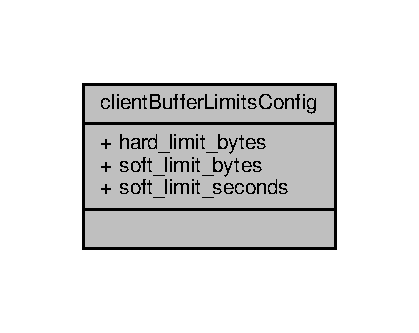
\includegraphics[width=201pt]{structclientBufferLimitsConfig__coll__graph}
\end{center}
\end{figure}
\subsection*{Data Fields}
\begin{DoxyCompactItemize}
\item 
\mbox{\Hypertarget{structclientBufferLimitsConfig_aae70a981b441e86c15bac720d09489d1}\label{structclientBufferLimitsConfig_aae70a981b441e86c15bac720d09489d1}} 
unsigned long long {\bfseries hard\+\_\+limit\+\_\+bytes}
\item 
\mbox{\Hypertarget{structclientBufferLimitsConfig_a902b5c41d03cc56b4ef0ceb40a43f9f3}\label{structclientBufferLimitsConfig_a902b5c41d03cc56b4ef0ceb40a43f9f3}} 
unsigned long long {\bfseries soft\+\_\+limit\+\_\+bytes}
\item 
\mbox{\Hypertarget{structclientBufferLimitsConfig_a50c38492435c6e133db45f4b2b79ce1d}\label{structclientBufferLimitsConfig_a50c38492435c6e133db45f4b2b79ce1d}} 
time\+\_\+t {\bfseries soft\+\_\+limit\+\_\+seconds}
\end{DoxyCompactItemize}


\subsection{Detailed Description}


Definition at line \hyperlink{server_8h_source_l00792}{792} of file \hyperlink{server_8h_source}{server.\+h}.



\subsection{Field Documentation}
\mbox{\Hypertarget{structclientBufferLimitsConfig_aae70a981b441e86c15bac720d09489d1}\label{structclientBufferLimitsConfig_aae70a981b441e86c15bac720d09489d1}} 
\index{client\+Buffer\+Limits\+Config@{client\+Buffer\+Limits\+Config}!hard\+\_\+limit\+\_\+bytes@{hard\+\_\+limit\+\_\+bytes}}
\index{hard\+\_\+limit\+\_\+bytes@{hard\+\_\+limit\+\_\+bytes}!client\+Buffer\+Limits\+Config@{client\+Buffer\+Limits\+Config}}
\subsubsection{\texorpdfstring{hard\+\_\+limit\+\_\+bytes}{hard\_limit\_bytes}}
{\footnotesize\ttfamily unsigned long long client\+Buffer\+Limits\+Config\+::hard\+\_\+limit\+\_\+bytes}



Definition at line \hyperlink{server_8h_source_l00793}{793} of file \hyperlink{server_8h_source}{server.\+h}.

\mbox{\Hypertarget{structclientBufferLimitsConfig_a902b5c41d03cc56b4ef0ceb40a43f9f3}\label{structclientBufferLimitsConfig_a902b5c41d03cc56b4ef0ceb40a43f9f3}} 
\index{client\+Buffer\+Limits\+Config@{client\+Buffer\+Limits\+Config}!soft\+\_\+limit\+\_\+bytes@{soft\+\_\+limit\+\_\+bytes}}
\index{soft\+\_\+limit\+\_\+bytes@{soft\+\_\+limit\+\_\+bytes}!client\+Buffer\+Limits\+Config@{client\+Buffer\+Limits\+Config}}
\subsubsection{\texorpdfstring{soft\+\_\+limit\+\_\+bytes}{soft\_limit\_bytes}}
{\footnotesize\ttfamily unsigned long long client\+Buffer\+Limits\+Config\+::soft\+\_\+limit\+\_\+bytes}



Definition at line \hyperlink{server_8h_source_l00794}{794} of file \hyperlink{server_8h_source}{server.\+h}.

\mbox{\Hypertarget{structclientBufferLimitsConfig_a50c38492435c6e133db45f4b2b79ce1d}\label{structclientBufferLimitsConfig_a50c38492435c6e133db45f4b2b79ce1d}} 
\index{client\+Buffer\+Limits\+Config@{client\+Buffer\+Limits\+Config}!soft\+\_\+limit\+\_\+seconds@{soft\+\_\+limit\+\_\+seconds}}
\index{soft\+\_\+limit\+\_\+seconds@{soft\+\_\+limit\+\_\+seconds}!client\+Buffer\+Limits\+Config@{client\+Buffer\+Limits\+Config}}
\subsubsection{\texorpdfstring{soft\+\_\+limit\+\_\+seconds}{soft\_limit\_seconds}}
{\footnotesize\ttfamily time\+\_\+t client\+Buffer\+Limits\+Config\+::soft\+\_\+limit\+\_\+seconds}



Definition at line \hyperlink{server_8h_source_l00795}{795} of file \hyperlink{server_8h_source}{server.\+h}.



The documentation for this struct was generated from the following file\+:\begin{DoxyCompactItemize}
\item 
src/server.\+h\end{DoxyCompactItemize}

\hypertarget{structclusterLink}{}\section{cluster\+Link Struct Reference}
\label{structclusterLink}\index{cluster\+Link@{cluster\+Link}}


Collaboration diagram for cluster\+Link\+:\nopagebreak
\begin{figure}[H]
\begin{center}
\leavevmode
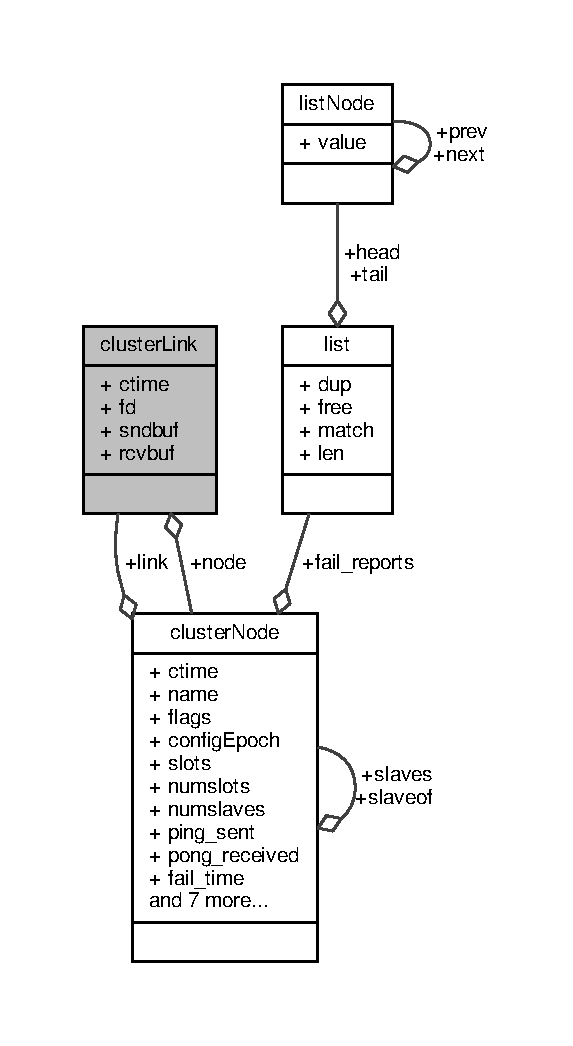
\includegraphics[width=275pt]{structclusterLink__coll__graph}
\end{center}
\end{figure}
\subsection*{Data Fields}
\begin{DoxyCompactItemize}
\item 
\mbox{\Hypertarget{structclusterLink_a69eb3bcdbd3b4f2d7b0e732c83644c17}\label{structclusterLink_a69eb3bcdbd3b4f2d7b0e732c83644c17}} 
mstime\+\_\+t {\bfseries ctime}
\item 
\mbox{\Hypertarget{structclusterLink_a97768f8f216e1325b79f89d32f385976}\label{structclusterLink_a97768f8f216e1325b79f89d32f385976}} 
int {\bfseries fd}
\item 
\mbox{\Hypertarget{structclusterLink_a18b2dfe01bf0cfb814944020ca6cef64}\label{structclusterLink_a18b2dfe01bf0cfb814944020ca6cef64}} 
sds {\bfseries sndbuf}
\item 
\mbox{\Hypertarget{structclusterLink_aa464832be4f8c9941ad3344918f25929}\label{structclusterLink_aa464832be4f8c9941ad3344918f25929}} 
sds {\bfseries rcvbuf}
\item 
\mbox{\Hypertarget{structclusterLink_af1afe49ebbbd6508d59bb4e56bbde563}\label{structclusterLink_af1afe49ebbbd6508d59bb4e56bbde563}} 
struct \hyperlink{structclusterNode}{cluster\+Node} $\ast$ {\bfseries node}
\end{DoxyCompactItemize}


\subsection{Detailed Description}


Definition at line \hyperlink{cluster_8h_source_l00040}{40} of file \hyperlink{cluster_8h_source}{cluster.\+h}.



\subsection{Field Documentation}
\mbox{\Hypertarget{structclusterLink_a69eb3bcdbd3b4f2d7b0e732c83644c17}\label{structclusterLink_a69eb3bcdbd3b4f2d7b0e732c83644c17}} 
\index{cluster\+Link@{cluster\+Link}!ctime@{ctime}}
\index{ctime@{ctime}!cluster\+Link@{cluster\+Link}}
\subsubsection{\texorpdfstring{ctime}{ctime}}
{\footnotesize\ttfamily mstime\+\_\+t cluster\+Link\+::ctime}



Definition at line \hyperlink{cluster_8h_source_l00041}{41} of file \hyperlink{cluster_8h_source}{cluster.\+h}.

\mbox{\Hypertarget{structclusterLink_a97768f8f216e1325b79f89d32f385976}\label{structclusterLink_a97768f8f216e1325b79f89d32f385976}} 
\index{cluster\+Link@{cluster\+Link}!fd@{fd}}
\index{fd@{fd}!cluster\+Link@{cluster\+Link}}
\subsubsection{\texorpdfstring{fd}{fd}}
{\footnotesize\ttfamily int cluster\+Link\+::fd}



Definition at line \hyperlink{cluster_8h_source_l00042}{42} of file \hyperlink{cluster_8h_source}{cluster.\+h}.

\mbox{\Hypertarget{structclusterLink_af1afe49ebbbd6508d59bb4e56bbde563}\label{structclusterLink_af1afe49ebbbd6508d59bb4e56bbde563}} 
\index{cluster\+Link@{cluster\+Link}!node@{node}}
\index{node@{node}!cluster\+Link@{cluster\+Link}}
\subsubsection{\texorpdfstring{node}{node}}
{\footnotesize\ttfamily struct \hyperlink{structclusterNode}{cluster\+Node}$\ast$ cluster\+Link\+::node}



Definition at line \hyperlink{cluster_8h_source_l00045}{45} of file \hyperlink{cluster_8h_source}{cluster.\+h}.

\mbox{\Hypertarget{structclusterLink_aa464832be4f8c9941ad3344918f25929}\label{structclusterLink_aa464832be4f8c9941ad3344918f25929}} 
\index{cluster\+Link@{cluster\+Link}!rcvbuf@{rcvbuf}}
\index{rcvbuf@{rcvbuf}!cluster\+Link@{cluster\+Link}}
\subsubsection{\texorpdfstring{rcvbuf}{rcvbuf}}
{\footnotesize\ttfamily sds cluster\+Link\+::rcvbuf}



Definition at line \hyperlink{cluster_8h_source_l00044}{44} of file \hyperlink{cluster_8h_source}{cluster.\+h}.

\mbox{\Hypertarget{structclusterLink_a18b2dfe01bf0cfb814944020ca6cef64}\label{structclusterLink_a18b2dfe01bf0cfb814944020ca6cef64}} 
\index{cluster\+Link@{cluster\+Link}!sndbuf@{sndbuf}}
\index{sndbuf@{sndbuf}!cluster\+Link@{cluster\+Link}}
\subsubsection{\texorpdfstring{sndbuf}{sndbuf}}
{\footnotesize\ttfamily sds cluster\+Link\+::sndbuf}



Definition at line \hyperlink{cluster_8h_source_l00043}{43} of file \hyperlink{cluster_8h_source}{cluster.\+h}.



The documentation for this struct was generated from the following file\+:\begin{DoxyCompactItemize}
\item 
src/cluster.\+h\end{DoxyCompactItemize}

\hypertarget{structclusterMsg}{}\section{cluster\+Msg Struct Reference}
\label{structclusterMsg}\index{cluster\+Msg@{cluster\+Msg}}


Collaboration diagram for cluster\+Msg\+:\nopagebreak
\begin{figure}[H]
\begin{center}
\leavevmode
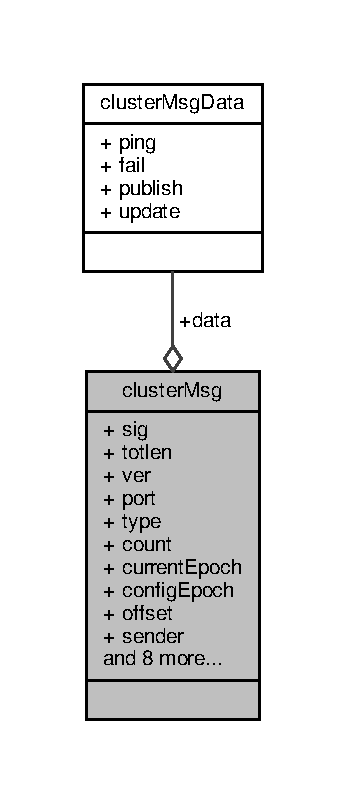
\includegraphics[width=166pt]{structclusterMsg__coll__graph}
\end{center}
\end{figure}
\subsection*{Data Fields}
\begin{DoxyCompactItemize}
\item 
\mbox{\Hypertarget{structclusterMsg_abb326313abd3ddb06eac6b9fd4273e96}\label{structclusterMsg_abb326313abd3ddb06eac6b9fd4273e96}} 
char {\bfseries sig} \mbox{[}4\mbox{]}
\item 
\mbox{\Hypertarget{structclusterMsg_a5ef56726841594a3d31e8d1f9db9cdc8}\label{structclusterMsg_a5ef56726841594a3d31e8d1f9db9cdc8}} 
uint32\+\_\+t {\bfseries totlen}
\item 
\mbox{\Hypertarget{structclusterMsg_a27c8382011859c9773f0303f59bac116}\label{structclusterMsg_a27c8382011859c9773f0303f59bac116}} 
uint16\+\_\+t {\bfseries ver}
\item 
\mbox{\Hypertarget{structclusterMsg_a610f1d78c588de5b3c3414f892e72974}\label{structclusterMsg_a610f1d78c588de5b3c3414f892e72974}} 
uint16\+\_\+t {\bfseries port}
\item 
\mbox{\Hypertarget{structclusterMsg_a06118df79b802adc033967b7d42ddd8c}\label{structclusterMsg_a06118df79b802adc033967b7d42ddd8c}} 
uint16\+\_\+t {\bfseries type}
\item 
\mbox{\Hypertarget{structclusterMsg_aba0776aac818854ae51ee0ed428d766b}\label{structclusterMsg_aba0776aac818854ae51ee0ed428d766b}} 
uint16\+\_\+t {\bfseries count}
\item 
\mbox{\Hypertarget{structclusterMsg_af587c060955ca4028c33087afaaceca4}\label{structclusterMsg_af587c060955ca4028c33087afaaceca4}} 
uint64\+\_\+t {\bfseries current\+Epoch}
\item 
\mbox{\Hypertarget{structclusterMsg_a45369d8251925dbda938652bf1f4438c}\label{structclusterMsg_a45369d8251925dbda938652bf1f4438c}} 
uint64\+\_\+t {\bfseries config\+Epoch}
\item 
\mbox{\Hypertarget{structclusterMsg_aa79837822db47e45154fc4ee08e3f246}\label{structclusterMsg_aa79837822db47e45154fc4ee08e3f246}} 
uint64\+\_\+t {\bfseries offset}
\item 
\mbox{\Hypertarget{structclusterMsg_acbf8f00d4c949073cb849d4f32ae6f53}\label{structclusterMsg_acbf8f00d4c949073cb849d4f32ae6f53}} 
char {\bfseries sender} \mbox{[}C\+L\+U\+S\+T\+E\+R\+\_\+\+N\+A\+M\+E\+L\+EN\mbox{]}
\item 
\mbox{\Hypertarget{structclusterMsg_a399581369cf6bda15a4ff0d06d72a119}\label{structclusterMsg_a399581369cf6bda15a4ff0d06d72a119}} 
unsigned char {\bfseries myslots} \mbox{[}C\+L\+U\+S\+T\+E\+R\+\_\+\+S\+L\+O\+TS/8\mbox{]}
\item 
\mbox{\Hypertarget{structclusterMsg_a5ca36f3f6316a0dfbf9ad4a1bbfdeb4a}\label{structclusterMsg_a5ca36f3f6316a0dfbf9ad4a1bbfdeb4a}} 
char {\bfseries slaveof} \mbox{[}C\+L\+U\+S\+T\+E\+R\+\_\+\+N\+A\+M\+E\+L\+EN\mbox{]}
\item 
\mbox{\Hypertarget{structclusterMsg_a4cecbddb92257abd32c3f3bfdb716614}\label{structclusterMsg_a4cecbddb92257abd32c3f3bfdb716614}} 
char {\bfseries myip} \mbox{[}N\+E\+T\+\_\+\+I\+P\+\_\+\+S\+T\+R\+\_\+\+L\+EN\mbox{]}
\item 
\mbox{\Hypertarget{structclusterMsg_a8f272476209e87783b2585bda0627912}\label{structclusterMsg_a8f272476209e87783b2585bda0627912}} 
char {\bfseries notused1} \mbox{[}34\mbox{]}
\item 
\mbox{\Hypertarget{structclusterMsg_a330ad2b74be19fa8130b5e5920d8c9fc}\label{structclusterMsg_a330ad2b74be19fa8130b5e5920d8c9fc}} 
uint16\+\_\+t {\bfseries cport}
\item 
\mbox{\Hypertarget{structclusterMsg_a2f5c02fb1d61410470cbfa32942fb745}\label{structclusterMsg_a2f5c02fb1d61410470cbfa32942fb745}} 
uint16\+\_\+t {\bfseries flags}
\item 
\mbox{\Hypertarget{structclusterMsg_a5cdfa214f48e21eb3ab2447acf18bc84}\label{structclusterMsg_a5cdfa214f48e21eb3ab2447acf18bc84}} 
unsigned char {\bfseries state}
\item 
\mbox{\Hypertarget{structclusterMsg_a1e6c3ad5211fb97e8ce03d35cc2ff747}\label{structclusterMsg_a1e6c3ad5211fb97e8ce03d35cc2ff747}} 
unsigned char {\bfseries mflags} \mbox{[}3\mbox{]}
\item 
\mbox{\Hypertarget{structclusterMsg_ae4a26a803883a1351225a9e12ede60a4}\label{structclusterMsg_ae4a26a803883a1351225a9e12ede60a4}} 
union \hyperlink{unionclusterMsgData}{cluster\+Msg\+Data} {\bfseries data}
\end{DoxyCompactItemize}


\subsection{Detailed Description}


Definition at line \hyperlink{cluster_8h_source_l00232}{232} of file \hyperlink{cluster_8h_source}{cluster.\+h}.



\subsection{Field Documentation}
\mbox{\Hypertarget{structclusterMsg_a45369d8251925dbda938652bf1f4438c}\label{structclusterMsg_a45369d8251925dbda938652bf1f4438c}} 
\index{cluster\+Msg@{cluster\+Msg}!config\+Epoch@{config\+Epoch}}
\index{config\+Epoch@{config\+Epoch}!cluster\+Msg@{cluster\+Msg}}
\subsubsection{\texorpdfstring{config\+Epoch}{configEpoch}}
{\footnotesize\ttfamily uint64\+\_\+t cluster\+Msg\+::config\+Epoch}



Definition at line \hyperlink{cluster_8h_source_l00240}{240} of file \hyperlink{cluster_8h_source}{cluster.\+h}.

\mbox{\Hypertarget{structclusterMsg_aba0776aac818854ae51ee0ed428d766b}\label{structclusterMsg_aba0776aac818854ae51ee0ed428d766b}} 
\index{cluster\+Msg@{cluster\+Msg}!count@{count}}
\index{count@{count}!cluster\+Msg@{cluster\+Msg}}
\subsubsection{\texorpdfstring{count}{count}}
{\footnotesize\ttfamily uint16\+\_\+t cluster\+Msg\+::count}



Definition at line \hyperlink{cluster_8h_source_l00238}{238} of file \hyperlink{cluster_8h_source}{cluster.\+h}.

\mbox{\Hypertarget{structclusterMsg_a330ad2b74be19fa8130b5e5920d8c9fc}\label{structclusterMsg_a330ad2b74be19fa8130b5e5920d8c9fc}} 
\index{cluster\+Msg@{cluster\+Msg}!cport@{cport}}
\index{cport@{cport}!cluster\+Msg@{cluster\+Msg}}
\subsubsection{\texorpdfstring{cport}{cport}}
{\footnotesize\ttfamily uint16\+\_\+t cluster\+Msg\+::cport}



Definition at line \hyperlink{cluster_8h_source_l00250}{250} of file \hyperlink{cluster_8h_source}{cluster.\+h}.

\mbox{\Hypertarget{structclusterMsg_af587c060955ca4028c33087afaaceca4}\label{structclusterMsg_af587c060955ca4028c33087afaaceca4}} 
\index{cluster\+Msg@{cluster\+Msg}!current\+Epoch@{current\+Epoch}}
\index{current\+Epoch@{current\+Epoch}!cluster\+Msg@{cluster\+Msg}}
\subsubsection{\texorpdfstring{current\+Epoch}{currentEpoch}}
{\footnotesize\ttfamily uint64\+\_\+t cluster\+Msg\+::current\+Epoch}



Definition at line \hyperlink{cluster_8h_source_l00239}{239} of file \hyperlink{cluster_8h_source}{cluster.\+h}.

\mbox{\Hypertarget{structclusterMsg_ae4a26a803883a1351225a9e12ede60a4}\label{structclusterMsg_ae4a26a803883a1351225a9e12ede60a4}} 
\index{cluster\+Msg@{cluster\+Msg}!data@{data}}
\index{data@{data}!cluster\+Msg@{cluster\+Msg}}
\subsubsection{\texorpdfstring{data}{data}}
{\footnotesize\ttfamily union \hyperlink{unionclusterMsgData}{cluster\+Msg\+Data} cluster\+Msg\+::data}



Definition at line \hyperlink{cluster_8h_source_l00254}{254} of file \hyperlink{cluster_8h_source}{cluster.\+h}.

\mbox{\Hypertarget{structclusterMsg_a2f5c02fb1d61410470cbfa32942fb745}\label{structclusterMsg_a2f5c02fb1d61410470cbfa32942fb745}} 
\index{cluster\+Msg@{cluster\+Msg}!flags@{flags}}
\index{flags@{flags}!cluster\+Msg@{cluster\+Msg}}
\subsubsection{\texorpdfstring{flags}{flags}}
{\footnotesize\ttfamily uint16\+\_\+t cluster\+Msg\+::flags}



Definition at line \hyperlink{cluster_8h_source_l00251}{251} of file \hyperlink{cluster_8h_source}{cluster.\+h}.

\mbox{\Hypertarget{structclusterMsg_a1e6c3ad5211fb97e8ce03d35cc2ff747}\label{structclusterMsg_a1e6c3ad5211fb97e8ce03d35cc2ff747}} 
\index{cluster\+Msg@{cluster\+Msg}!mflags@{mflags}}
\index{mflags@{mflags}!cluster\+Msg@{cluster\+Msg}}
\subsubsection{\texorpdfstring{mflags}{mflags}}
{\footnotesize\ttfamily unsigned char cluster\+Msg\+::mflags\mbox{[}3\mbox{]}}



Definition at line \hyperlink{cluster_8h_source_l00253}{253} of file \hyperlink{cluster_8h_source}{cluster.\+h}.

\mbox{\Hypertarget{structclusterMsg_a4cecbddb92257abd32c3f3bfdb716614}\label{structclusterMsg_a4cecbddb92257abd32c3f3bfdb716614}} 
\index{cluster\+Msg@{cluster\+Msg}!myip@{myip}}
\index{myip@{myip}!cluster\+Msg@{cluster\+Msg}}
\subsubsection{\texorpdfstring{myip}{myip}}
{\footnotesize\ttfamily char cluster\+Msg\+::myip\mbox{[}N\+E\+T\+\_\+\+I\+P\+\_\+\+S\+T\+R\+\_\+\+L\+EN\mbox{]}}



Definition at line \hyperlink{cluster_8h_source_l00248}{248} of file \hyperlink{cluster_8h_source}{cluster.\+h}.

\mbox{\Hypertarget{structclusterMsg_a399581369cf6bda15a4ff0d06d72a119}\label{structclusterMsg_a399581369cf6bda15a4ff0d06d72a119}} 
\index{cluster\+Msg@{cluster\+Msg}!myslots@{myslots}}
\index{myslots@{myslots}!cluster\+Msg@{cluster\+Msg}}
\subsubsection{\texorpdfstring{myslots}{myslots}}
{\footnotesize\ttfamily unsigned char cluster\+Msg\+::myslots\mbox{[}C\+L\+U\+S\+T\+E\+R\+\_\+\+S\+L\+O\+TS/8\mbox{]}}



Definition at line \hyperlink{cluster_8h_source_l00246}{246} of file \hyperlink{cluster_8h_source}{cluster.\+h}.

\mbox{\Hypertarget{structclusterMsg_a8f272476209e87783b2585bda0627912}\label{structclusterMsg_a8f272476209e87783b2585bda0627912}} 
\index{cluster\+Msg@{cluster\+Msg}!notused1@{notused1}}
\index{notused1@{notused1}!cluster\+Msg@{cluster\+Msg}}
\subsubsection{\texorpdfstring{notused1}{notused1}}
{\footnotesize\ttfamily char cluster\+Msg\+::notused1\mbox{[}34\mbox{]}}



Definition at line \hyperlink{cluster_8h_source_l00249}{249} of file \hyperlink{cluster_8h_source}{cluster.\+h}.

\mbox{\Hypertarget{structclusterMsg_aa79837822db47e45154fc4ee08e3f246}\label{structclusterMsg_aa79837822db47e45154fc4ee08e3f246}} 
\index{cluster\+Msg@{cluster\+Msg}!offset@{offset}}
\index{offset@{offset}!cluster\+Msg@{cluster\+Msg}}
\subsubsection{\texorpdfstring{offset}{offset}}
{\footnotesize\ttfamily uint64\+\_\+t cluster\+Msg\+::offset}



Definition at line \hyperlink{cluster_8h_source_l00243}{243} of file \hyperlink{cluster_8h_source}{cluster.\+h}.

\mbox{\Hypertarget{structclusterMsg_a610f1d78c588de5b3c3414f892e72974}\label{structclusterMsg_a610f1d78c588de5b3c3414f892e72974}} 
\index{cluster\+Msg@{cluster\+Msg}!port@{port}}
\index{port@{port}!cluster\+Msg@{cluster\+Msg}}
\subsubsection{\texorpdfstring{port}{port}}
{\footnotesize\ttfamily uint16\+\_\+t cluster\+Msg\+::port}



Definition at line \hyperlink{cluster_8h_source_l00236}{236} of file \hyperlink{cluster_8h_source}{cluster.\+h}.

\mbox{\Hypertarget{structclusterMsg_acbf8f00d4c949073cb849d4f32ae6f53}\label{structclusterMsg_acbf8f00d4c949073cb849d4f32ae6f53}} 
\index{cluster\+Msg@{cluster\+Msg}!sender@{sender}}
\index{sender@{sender}!cluster\+Msg@{cluster\+Msg}}
\subsubsection{\texorpdfstring{sender}{sender}}
{\footnotesize\ttfamily char cluster\+Msg\+::sender\mbox{[}C\+L\+U\+S\+T\+E\+R\+\_\+\+N\+A\+M\+E\+L\+EN\mbox{]}}



Definition at line \hyperlink{cluster_8h_source_l00245}{245} of file \hyperlink{cluster_8h_source}{cluster.\+h}.

\mbox{\Hypertarget{structclusterMsg_abb326313abd3ddb06eac6b9fd4273e96}\label{structclusterMsg_abb326313abd3ddb06eac6b9fd4273e96}} 
\index{cluster\+Msg@{cluster\+Msg}!sig@{sig}}
\index{sig@{sig}!cluster\+Msg@{cluster\+Msg}}
\subsubsection{\texorpdfstring{sig}{sig}}
{\footnotesize\ttfamily char cluster\+Msg\+::sig\mbox{[}4\mbox{]}}



Definition at line \hyperlink{cluster_8h_source_l00233}{233} of file \hyperlink{cluster_8h_source}{cluster.\+h}.

\mbox{\Hypertarget{structclusterMsg_a5ca36f3f6316a0dfbf9ad4a1bbfdeb4a}\label{structclusterMsg_a5ca36f3f6316a0dfbf9ad4a1bbfdeb4a}} 
\index{cluster\+Msg@{cluster\+Msg}!slaveof@{slaveof}}
\index{slaveof@{slaveof}!cluster\+Msg@{cluster\+Msg}}
\subsubsection{\texorpdfstring{slaveof}{slaveof}}
{\footnotesize\ttfamily char cluster\+Msg\+::slaveof\mbox{[}C\+L\+U\+S\+T\+E\+R\+\_\+\+N\+A\+M\+E\+L\+EN\mbox{]}}



Definition at line \hyperlink{cluster_8h_source_l00247}{247} of file \hyperlink{cluster_8h_source}{cluster.\+h}.

\mbox{\Hypertarget{structclusterMsg_a5cdfa214f48e21eb3ab2447acf18bc84}\label{structclusterMsg_a5cdfa214f48e21eb3ab2447acf18bc84}} 
\index{cluster\+Msg@{cluster\+Msg}!state@{state}}
\index{state@{state}!cluster\+Msg@{cluster\+Msg}}
\subsubsection{\texorpdfstring{state}{state}}
{\footnotesize\ttfamily unsigned char cluster\+Msg\+::state}



Definition at line \hyperlink{cluster_8h_source_l00252}{252} of file \hyperlink{cluster_8h_source}{cluster.\+h}.

\mbox{\Hypertarget{structclusterMsg_a5ef56726841594a3d31e8d1f9db9cdc8}\label{structclusterMsg_a5ef56726841594a3d31e8d1f9db9cdc8}} 
\index{cluster\+Msg@{cluster\+Msg}!totlen@{totlen}}
\index{totlen@{totlen}!cluster\+Msg@{cluster\+Msg}}
\subsubsection{\texorpdfstring{totlen}{totlen}}
{\footnotesize\ttfamily uint32\+\_\+t cluster\+Msg\+::totlen}



Definition at line \hyperlink{cluster_8h_source_l00234}{234} of file \hyperlink{cluster_8h_source}{cluster.\+h}.

\mbox{\Hypertarget{structclusterMsg_a06118df79b802adc033967b7d42ddd8c}\label{structclusterMsg_a06118df79b802adc033967b7d42ddd8c}} 
\index{cluster\+Msg@{cluster\+Msg}!type@{type}}
\index{type@{type}!cluster\+Msg@{cluster\+Msg}}
\subsubsection{\texorpdfstring{type}{type}}
{\footnotesize\ttfamily uint16\+\_\+t cluster\+Msg\+::type}



Definition at line \hyperlink{cluster_8h_source_l00237}{237} of file \hyperlink{cluster_8h_source}{cluster.\+h}.

\mbox{\Hypertarget{structclusterMsg_a27c8382011859c9773f0303f59bac116}\label{structclusterMsg_a27c8382011859c9773f0303f59bac116}} 
\index{cluster\+Msg@{cluster\+Msg}!ver@{ver}}
\index{ver@{ver}!cluster\+Msg@{cluster\+Msg}}
\subsubsection{\texorpdfstring{ver}{ver}}
{\footnotesize\ttfamily uint16\+\_\+t cluster\+Msg\+::ver}



Definition at line \hyperlink{cluster_8h_source_l00235}{235} of file \hyperlink{cluster_8h_source}{cluster.\+h}.



The documentation for this struct was generated from the following file\+:\begin{DoxyCompactItemize}
\item 
src/cluster.\+h\end{DoxyCompactItemize}

\hypertarget{unionclusterMsgData}{}\section{cluster\+Msg\+Data Union Reference}
\label{unionclusterMsgData}\index{cluster\+Msg\+Data@{cluster\+Msg\+Data}}


Collaboration diagram for cluster\+Msg\+Data\+:\nopagebreak
\begin{figure}[H]
\begin{center}
\leavevmode
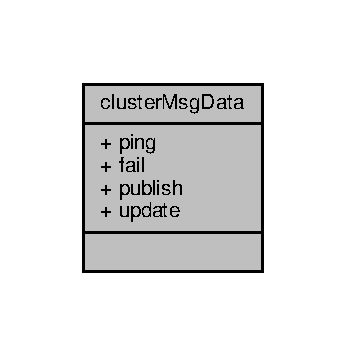
\includegraphics[width=166pt]{unionclusterMsgData__coll__graph}
\end{center}
\end{figure}
\subsection*{Data Fields}
\begin{DoxyCompactItemize}
\item 
\mbox{\Hypertarget{unionclusterMsgData_a7a5842b1f4b4e026c41a98768b5889f4}\label{unionclusterMsgData_a7a5842b1f4b4e026c41a98768b5889f4}} 
\begin{tabbing}
xx\=xx\=xx\=xx\=xx\=xx\=xx\=xx\=xx\=\kill
struct \{\\
\mbox{\Hypertarget{unionclusterMsgData_ad53c42a54a807972cc7da21616cf601c}\label{unionclusterMsgData_ad53c42a54a807972cc7da21616cf601c}} 
\hyperlink{structclusterMsgDataGossip}{clusterMsgDataGossip} {\bfseries gossip} \mbox{[}1\mbox{]}\\
\} {\bfseries ping}\\

\end{tabbing}\item 
\mbox{\Hypertarget{unionclusterMsgData_abad9fafed8c8896b318124af266e99ef}\label{unionclusterMsgData_abad9fafed8c8896b318124af266e99ef}} 
\begin{tabbing}
xx\=xx\=xx\=xx\=xx\=xx\=xx\=xx\=xx\=\kill
struct \{\\
\mbox{\Hypertarget{unionclusterMsgData_aa0b773e79b54f8c7b917a57d797047f0}\label{unionclusterMsgData_aa0b773e79b54f8c7b917a57d797047f0}} 
\hyperlink{structclusterMsgDataFail}{clusterMsgDataFail} {\bfseries about}\\
\} {\bfseries fail}\\

\end{tabbing}\item 
\mbox{\Hypertarget{unionclusterMsgData_a3db1b1663d248a76e1a8bd88449b0823}\label{unionclusterMsgData_a3db1b1663d248a76e1a8bd88449b0823}} 
\begin{tabbing}
xx\=xx\=xx\=xx\=xx\=xx\=xx\=xx\=xx\=\kill
struct \{\\
\mbox{\Hypertarget{unionclusterMsgData_af9c7424cbfae93d958bf4fd1a8c7ba62}\label{unionclusterMsgData_af9c7424cbfae93d958bf4fd1a8c7ba62}} 
\hyperlink{structclusterMsgDataPublish}{clusterMsgDataPublish} {\bfseries msg}\\
\} {\bfseries publish}\\

\end{tabbing}\item 
\mbox{\Hypertarget{unionclusterMsgData_af91b32a2f7cec8a5b3d4d32ed3685fbd}\label{unionclusterMsgData_af91b32a2f7cec8a5b3d4d32ed3685fbd}} 
\begin{tabbing}
xx\=xx\=xx\=xx\=xx\=xx\=xx\=xx\=xx\=\kill
struct \{\\
\mbox{\Hypertarget{unionclusterMsgData_a9f502b25c2444e1a9fe2ffdf21a732ae}\label{unionclusterMsgData_a9f502b25c2444e1a9fe2ffdf21a732ae}} 
\hyperlink{structclusterMsgDataUpdate}{clusterMsgDataUpdate} {\bfseries nodecfg}\\
\} {\bfseries update}\\

\end{tabbing}\end{DoxyCompactItemize}


\subsection{Detailed Description}


Definition at line \hyperlink{cluster_8h_source_l00207}{207} of file \hyperlink{cluster_8h_source}{cluster.\+h}.



\subsection{Field Documentation}
\mbox{\Hypertarget{unionclusterMsgData_abad9fafed8c8896b318124af266e99ef}\label{unionclusterMsgData_abad9fafed8c8896b318124af266e99ef}} 
\index{cluster\+Msg\+Data@{cluster\+Msg\+Data}!fail@{fail}}
\index{fail@{fail}!cluster\+Msg\+Data@{cluster\+Msg\+Data}}
\subsubsection{\texorpdfstring{fail}{fail}}
{\footnotesize\ttfamily struct \{ ... \}   cluster\+Msg\+Data\+::fail}

\mbox{\Hypertarget{unionclusterMsgData_a7a5842b1f4b4e026c41a98768b5889f4}\label{unionclusterMsgData_a7a5842b1f4b4e026c41a98768b5889f4}} 
\index{cluster\+Msg\+Data@{cluster\+Msg\+Data}!ping@{ping}}
\index{ping@{ping}!cluster\+Msg\+Data@{cluster\+Msg\+Data}}
\subsubsection{\texorpdfstring{ping}{ping}}
{\footnotesize\ttfamily struct \{ ... \}   cluster\+Msg\+Data\+::ping}

\mbox{\Hypertarget{unionclusterMsgData_a3db1b1663d248a76e1a8bd88449b0823}\label{unionclusterMsgData_a3db1b1663d248a76e1a8bd88449b0823}} 
\index{cluster\+Msg\+Data@{cluster\+Msg\+Data}!publish@{publish}}
\index{publish@{publish}!cluster\+Msg\+Data@{cluster\+Msg\+Data}}
\subsubsection{\texorpdfstring{publish}{publish}}
{\footnotesize\ttfamily struct \{ ... \}   cluster\+Msg\+Data\+::publish}

\mbox{\Hypertarget{unionclusterMsgData_af91b32a2f7cec8a5b3d4d32ed3685fbd}\label{unionclusterMsgData_af91b32a2f7cec8a5b3d4d32ed3685fbd}} 
\index{cluster\+Msg\+Data@{cluster\+Msg\+Data}!update@{update}}
\index{update@{update}!cluster\+Msg\+Data@{cluster\+Msg\+Data}}
\subsubsection{\texorpdfstring{update}{update}}
{\footnotesize\ttfamily struct \{ ... \}   cluster\+Msg\+Data\+::update}



The documentation for this union was generated from the following file\+:\begin{DoxyCompactItemize}
\item 
src/cluster.\+h\end{DoxyCompactItemize}

\hypertarget{structclusterMsgData_8fail}{}\section{cluster\+Msg\+Data.\+fail Struct Reference}
\label{structclusterMsgData_8fail}\index{cluster\+Msg\+Data.\+fail@{cluster\+Msg\+Data.\+fail}}


Collaboration diagram for cluster\+Msg\+Data.\+fail\+:\nopagebreak
\begin{figure}[H]
\begin{center}
\leavevmode
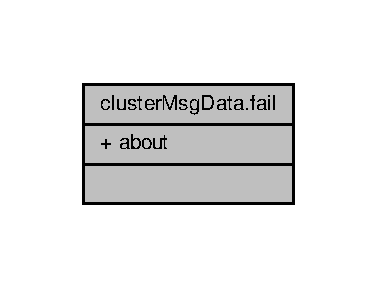
\includegraphics[width=181pt]{structclusterMsgData_8fail__coll__graph}
\end{center}
\end{figure}
\subsection*{Data Fields}
\begin{DoxyCompactItemize}
\item 
\mbox{\Hypertarget{structclusterMsgData_8fail_a46b3931b9959c927df4fc65fdee94b07}\label{structclusterMsgData_8fail_a46b3931b9959c927df4fc65fdee94b07}} 
\hyperlink{structclusterMsgDataFail}{cluster\+Msg\+Data\+Fail} {\bfseries about}
\end{DoxyCompactItemize}


\subsection{Detailed Description}


Definition at line \hyperlink{cluster_8h_source_l00215}{215} of file \hyperlink{cluster_8h_source}{cluster.\+h}.



\subsection{Field Documentation}
\mbox{\Hypertarget{structclusterMsgData_8fail_a46b3931b9959c927df4fc65fdee94b07}\label{structclusterMsgData_8fail_a46b3931b9959c927df4fc65fdee94b07}} 
\index{cluster\+Msg\+Data.\+fail@{cluster\+Msg\+Data.\+fail}!about@{about}}
\index{about@{about}!cluster\+Msg\+Data.\+fail@{cluster\+Msg\+Data.\+fail}}
\subsubsection{\texorpdfstring{about}{about}}
{\footnotesize\ttfamily }



The documentation for this struct was generated from the following files\+:
\hypertarget{structclusterMsgData_8ping}{}\section{cluster\+Msg\+Data.\+ping Struct Reference}
\label{structclusterMsgData_8ping}\index{cluster\+Msg\+Data.\+ping@{cluster\+Msg\+Data.\+ping}}


Collaboration diagram for cluster\+Msg\+Data.\+ping\+:\nopagebreak
\begin{figure}[H]
\begin{center}
\leavevmode
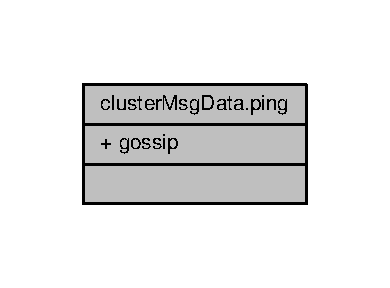
\includegraphics[width=187pt]{structclusterMsgData_8ping__coll__graph}
\end{center}
\end{figure}
\subsection*{Data Fields}
\begin{DoxyCompactItemize}
\item 
\mbox{\Hypertarget{structclusterMsgData_8ping_a9c226c311c450e8f0a4ca6a8430721c8}\label{structclusterMsgData_8ping_a9c226c311c450e8f0a4ca6a8430721c8}} 
\hyperlink{structclusterMsgDataGossip}{cluster\+Msg\+Data\+Gossip} {\bfseries gossip} \mbox{[}1\mbox{]}
\end{DoxyCompactItemize}


\subsection{Detailed Description}


Definition at line \hyperlink{cluster_8h_source_l00209}{209} of file \hyperlink{cluster_8h_source}{cluster.\+h}.



\subsection{Field Documentation}
\mbox{\Hypertarget{structclusterMsgData_8ping_a9c226c311c450e8f0a4ca6a8430721c8}\label{structclusterMsgData_8ping_a9c226c311c450e8f0a4ca6a8430721c8}} 
\index{cluster\+Msg\+Data.\+ping@{cluster\+Msg\+Data.\+ping}!gossip@{gossip}}
\index{gossip@{gossip}!cluster\+Msg\+Data.\+ping@{cluster\+Msg\+Data.\+ping}}
\subsubsection{\texorpdfstring{gossip}{gossip}}
{\footnotesize\ttfamily }



The documentation for this struct was generated from the following files\+:
\hypertarget{structclusterMsgData_8publish}{}\section{cluster\+Msg\+Data.\+publish Struct Reference}
\label{structclusterMsgData_8publish}\index{cluster\+Msg\+Data.\+publish@{cluster\+Msg\+Data.\+publish}}


Collaboration diagram for cluster\+Msg\+Data.\+publish\+:\nopagebreak
\begin{figure}[H]
\begin{center}
\leavevmode
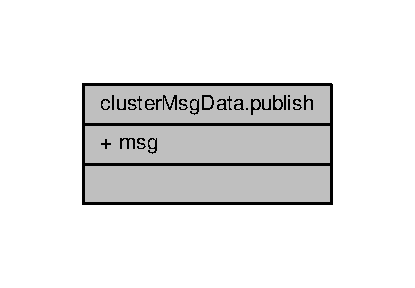
\includegraphics[width=199pt]{structclusterMsgData_8publish__coll__graph}
\end{center}
\end{figure}
\subsection*{Data Fields}
\begin{DoxyCompactItemize}
\item 
\mbox{\Hypertarget{structclusterMsgData_8publish_a6e2baaf3b97dbeef01c0043275f9a0e7}\label{structclusterMsgData_8publish_a6e2baaf3b97dbeef01c0043275f9a0e7}} 
\hyperlink{structclusterMsgDataPublish}{cluster\+Msg\+Data\+Publish} {\bfseries msg}
\end{DoxyCompactItemize}


\subsection{Detailed Description}


Definition at line \hyperlink{cluster_8h_source_l00220}{220} of file \hyperlink{cluster_8h_source}{cluster.\+h}.



\subsection{Field Documentation}
\mbox{\Hypertarget{structclusterMsgData_8publish_a6e2baaf3b97dbeef01c0043275f9a0e7}\label{structclusterMsgData_8publish_a6e2baaf3b97dbeef01c0043275f9a0e7}} 
\index{cluster\+Msg\+Data.\+publish@{cluster\+Msg\+Data.\+publish}!msg@{msg}}
\index{msg@{msg}!cluster\+Msg\+Data.\+publish@{cluster\+Msg\+Data.\+publish}}
\subsubsection{\texorpdfstring{msg}{msg}}
{\footnotesize\ttfamily }



The documentation for this struct was generated from the following files\+:
\hypertarget{structclusterMsgData_8update}{}\section{cluster\+Msg\+Data.\+update Struct Reference}
\label{structclusterMsgData_8update}\index{cluster\+Msg\+Data.\+update@{cluster\+Msg\+Data.\+update}}


Collaboration diagram for cluster\+Msg\+Data.\+update\+:\nopagebreak
\begin{figure}[H]
\begin{center}
\leavevmode
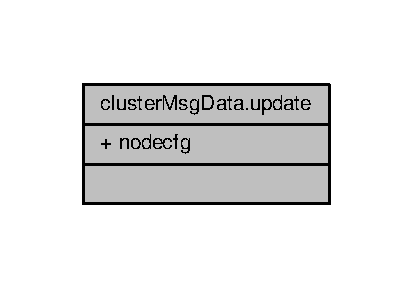
\includegraphics[width=198pt]{structclusterMsgData_8update__coll__graph}
\end{center}
\end{figure}
\subsection*{Data Fields}
\begin{DoxyCompactItemize}
\item 
\mbox{\Hypertarget{structclusterMsgData_8update_a062ab3f657fd3b5fb7a452a0fb5bcd74}\label{structclusterMsgData_8update_a062ab3f657fd3b5fb7a452a0fb5bcd74}} 
\hyperlink{structclusterMsgDataUpdate}{cluster\+Msg\+Data\+Update} {\bfseries nodecfg}
\end{DoxyCompactItemize}


\subsection{Detailed Description}


Definition at line \hyperlink{cluster_8h_source_l00225}{225} of file \hyperlink{cluster_8h_source}{cluster.\+h}.



\subsection{Field Documentation}
\mbox{\Hypertarget{structclusterMsgData_8update_a062ab3f657fd3b5fb7a452a0fb5bcd74}\label{structclusterMsgData_8update_a062ab3f657fd3b5fb7a452a0fb5bcd74}} 
\index{cluster\+Msg\+Data.\+update@{cluster\+Msg\+Data.\+update}!nodecfg@{nodecfg}}
\index{nodecfg@{nodecfg}!cluster\+Msg\+Data.\+update@{cluster\+Msg\+Data.\+update}}
\subsubsection{\texorpdfstring{nodecfg}{nodecfg}}
{\footnotesize\ttfamily }



The documentation for this struct was generated from the following files\+:
\hypertarget{structclusterMsgDataFail}{}\section{cluster\+Msg\+Data\+Fail Struct Reference}
\label{structclusterMsgDataFail}\index{cluster\+Msg\+Data\+Fail@{cluster\+Msg\+Data\+Fail}}


Collaboration diagram for cluster\+Msg\+Data\+Fail\+:\nopagebreak
\begin{figure}[H]
\begin{center}
\leavevmode
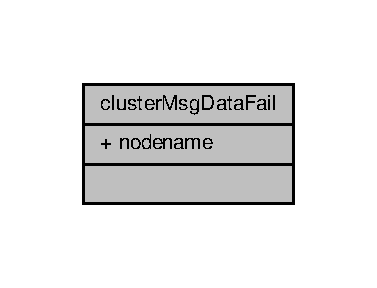
\includegraphics[width=181pt]{structclusterMsgDataFail__coll__graph}
\end{center}
\end{figure}
\subsection*{Data Fields}
\begin{DoxyCompactItemize}
\item 
\mbox{\Hypertarget{structclusterMsgDataFail_aca019d47dd052819120b85344ecfbd30}\label{structclusterMsgDataFail_aca019d47dd052819120b85344ecfbd30}} 
char {\bfseries nodename} \mbox{[}C\+L\+U\+S\+T\+E\+R\+\_\+\+N\+A\+M\+E\+L\+EN\mbox{]}
\end{DoxyCompactItemize}


\subsection{Detailed Description}


Definition at line \hyperlink{cluster_8h_source_l00188}{188} of file \hyperlink{cluster_8h_source}{cluster.\+h}.



\subsection{Field Documentation}
\mbox{\Hypertarget{structclusterMsgDataFail_aca019d47dd052819120b85344ecfbd30}\label{structclusterMsgDataFail_aca019d47dd052819120b85344ecfbd30}} 
\index{cluster\+Msg\+Data\+Fail@{cluster\+Msg\+Data\+Fail}!nodename@{nodename}}
\index{nodename@{nodename}!cluster\+Msg\+Data\+Fail@{cluster\+Msg\+Data\+Fail}}
\subsubsection{\texorpdfstring{nodename}{nodename}}
{\footnotesize\ttfamily char cluster\+Msg\+Data\+Fail\+::nodename\mbox{[}C\+L\+U\+S\+T\+E\+R\+\_\+\+N\+A\+M\+E\+L\+EN\mbox{]}}



Definition at line \hyperlink{cluster_8h_source_l00189}{189} of file \hyperlink{cluster_8h_source}{cluster.\+h}.



The documentation for this struct was generated from the following file\+:\begin{DoxyCompactItemize}
\item 
src/cluster.\+h\end{DoxyCompactItemize}

\hypertarget{structclusterMsgDataGossip}{}\section{cluster\+Msg\+Data\+Gossip Struct Reference}
\label{structclusterMsgDataGossip}\index{cluster\+Msg\+Data\+Gossip@{cluster\+Msg\+Data\+Gossip}}


Collaboration diagram for cluster\+Msg\+Data\+Gossip\+:\nopagebreak
\begin{figure}[H]
\begin{center}
\leavevmode
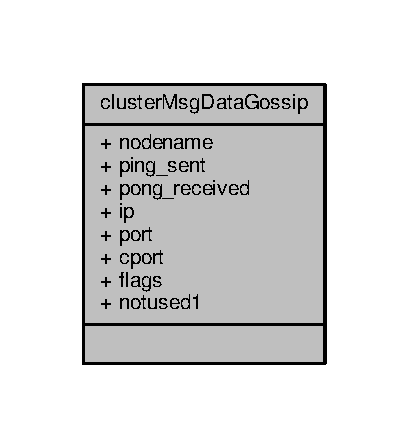
\includegraphics[width=196pt]{structclusterMsgDataGossip__coll__graph}
\end{center}
\end{figure}
\subsection*{Data Fields}
\begin{DoxyCompactItemize}
\item 
\mbox{\Hypertarget{structclusterMsgDataGossip_a382a71f82a25f5db3d72cc157e5e7df7}\label{structclusterMsgDataGossip_a382a71f82a25f5db3d72cc157e5e7df7}} 
char {\bfseries nodename} \mbox{[}C\+L\+U\+S\+T\+E\+R\+\_\+\+N\+A\+M\+E\+L\+EN\mbox{]}
\item 
\mbox{\Hypertarget{structclusterMsgDataGossip_afca2b0fa134954fc8e0652a1e35eaa35}\label{structclusterMsgDataGossip_afca2b0fa134954fc8e0652a1e35eaa35}} 
uint32\+\_\+t {\bfseries ping\+\_\+sent}
\item 
\mbox{\Hypertarget{structclusterMsgDataGossip_acd8f681b7d76d00bf70d27b1130c97df}\label{structclusterMsgDataGossip_acd8f681b7d76d00bf70d27b1130c97df}} 
uint32\+\_\+t {\bfseries pong\+\_\+received}
\item 
\mbox{\Hypertarget{structclusterMsgDataGossip_ad1f61e0cc5f9be1db6aa4cd7c85c554a}\label{structclusterMsgDataGossip_ad1f61e0cc5f9be1db6aa4cd7c85c554a}} 
char {\bfseries ip} \mbox{[}N\+E\+T\+\_\+\+I\+P\+\_\+\+S\+T\+R\+\_\+\+L\+EN\mbox{]}
\item 
\mbox{\Hypertarget{structclusterMsgDataGossip_a6a38835f189c60b4c9ea9be5c817e6af}\label{structclusterMsgDataGossip_a6a38835f189c60b4c9ea9be5c817e6af}} 
uint16\+\_\+t {\bfseries port}
\item 
\mbox{\Hypertarget{structclusterMsgDataGossip_a2e1abb299507da7c3f6b56235a9ad1f5}\label{structclusterMsgDataGossip_a2e1abb299507da7c3f6b56235a9ad1f5}} 
uint16\+\_\+t {\bfseries cport}
\item 
\mbox{\Hypertarget{structclusterMsgDataGossip_ad1ca60d86c831ae3592f10f1632c71e1}\label{structclusterMsgDataGossip_ad1ca60d86c831ae3592f10f1632c71e1}} 
uint16\+\_\+t {\bfseries flags}
\item 
\mbox{\Hypertarget{structclusterMsgDataGossip_a84dfb60c8d76dc947d5940c18d290403}\label{structclusterMsgDataGossip_a84dfb60c8d76dc947d5940c18d290403}} 
uint32\+\_\+t {\bfseries notused1}
\end{DoxyCompactItemize}


\subsection{Detailed Description}


Definition at line \hyperlink{cluster_8h_source_l00177}{177} of file \hyperlink{cluster_8h_source}{cluster.\+h}.



\subsection{Field Documentation}
\mbox{\Hypertarget{structclusterMsgDataGossip_a2e1abb299507da7c3f6b56235a9ad1f5}\label{structclusterMsgDataGossip_a2e1abb299507da7c3f6b56235a9ad1f5}} 
\index{cluster\+Msg\+Data\+Gossip@{cluster\+Msg\+Data\+Gossip}!cport@{cport}}
\index{cport@{cport}!cluster\+Msg\+Data\+Gossip@{cluster\+Msg\+Data\+Gossip}}
\subsubsection{\texorpdfstring{cport}{cport}}
{\footnotesize\ttfamily uint16\+\_\+t cluster\+Msg\+Data\+Gossip\+::cport}



Definition at line \hyperlink{cluster_8h_source_l00183}{183} of file \hyperlink{cluster_8h_source}{cluster.\+h}.

\mbox{\Hypertarget{structclusterMsgDataGossip_ad1ca60d86c831ae3592f10f1632c71e1}\label{structclusterMsgDataGossip_ad1ca60d86c831ae3592f10f1632c71e1}} 
\index{cluster\+Msg\+Data\+Gossip@{cluster\+Msg\+Data\+Gossip}!flags@{flags}}
\index{flags@{flags}!cluster\+Msg\+Data\+Gossip@{cluster\+Msg\+Data\+Gossip}}
\subsubsection{\texorpdfstring{flags}{flags}}
{\footnotesize\ttfamily uint16\+\_\+t cluster\+Msg\+Data\+Gossip\+::flags}



Definition at line \hyperlink{cluster_8h_source_l00184}{184} of file \hyperlink{cluster_8h_source}{cluster.\+h}.

\mbox{\Hypertarget{structclusterMsgDataGossip_ad1f61e0cc5f9be1db6aa4cd7c85c554a}\label{structclusterMsgDataGossip_ad1f61e0cc5f9be1db6aa4cd7c85c554a}} 
\index{cluster\+Msg\+Data\+Gossip@{cluster\+Msg\+Data\+Gossip}!ip@{ip}}
\index{ip@{ip}!cluster\+Msg\+Data\+Gossip@{cluster\+Msg\+Data\+Gossip}}
\subsubsection{\texorpdfstring{ip}{ip}}
{\footnotesize\ttfamily char cluster\+Msg\+Data\+Gossip\+::ip\mbox{[}N\+E\+T\+\_\+\+I\+P\+\_\+\+S\+T\+R\+\_\+\+L\+EN\mbox{]}}



Definition at line \hyperlink{cluster_8h_source_l00181}{181} of file \hyperlink{cluster_8h_source}{cluster.\+h}.

\mbox{\Hypertarget{structclusterMsgDataGossip_a382a71f82a25f5db3d72cc157e5e7df7}\label{structclusterMsgDataGossip_a382a71f82a25f5db3d72cc157e5e7df7}} 
\index{cluster\+Msg\+Data\+Gossip@{cluster\+Msg\+Data\+Gossip}!nodename@{nodename}}
\index{nodename@{nodename}!cluster\+Msg\+Data\+Gossip@{cluster\+Msg\+Data\+Gossip}}
\subsubsection{\texorpdfstring{nodename}{nodename}}
{\footnotesize\ttfamily char cluster\+Msg\+Data\+Gossip\+::nodename\mbox{[}C\+L\+U\+S\+T\+E\+R\+\_\+\+N\+A\+M\+E\+L\+EN\mbox{]}}



Definition at line \hyperlink{cluster_8h_source_l00178}{178} of file \hyperlink{cluster_8h_source}{cluster.\+h}.

\mbox{\Hypertarget{structclusterMsgDataGossip_a84dfb60c8d76dc947d5940c18d290403}\label{structclusterMsgDataGossip_a84dfb60c8d76dc947d5940c18d290403}} 
\index{cluster\+Msg\+Data\+Gossip@{cluster\+Msg\+Data\+Gossip}!notused1@{notused1}}
\index{notused1@{notused1}!cluster\+Msg\+Data\+Gossip@{cluster\+Msg\+Data\+Gossip}}
\subsubsection{\texorpdfstring{notused1}{notused1}}
{\footnotesize\ttfamily uint32\+\_\+t cluster\+Msg\+Data\+Gossip\+::notused1}



Definition at line \hyperlink{cluster_8h_source_l00185}{185} of file \hyperlink{cluster_8h_source}{cluster.\+h}.

\mbox{\Hypertarget{structclusterMsgDataGossip_afca2b0fa134954fc8e0652a1e35eaa35}\label{structclusterMsgDataGossip_afca2b0fa134954fc8e0652a1e35eaa35}} 
\index{cluster\+Msg\+Data\+Gossip@{cluster\+Msg\+Data\+Gossip}!ping\+\_\+sent@{ping\+\_\+sent}}
\index{ping\+\_\+sent@{ping\+\_\+sent}!cluster\+Msg\+Data\+Gossip@{cluster\+Msg\+Data\+Gossip}}
\subsubsection{\texorpdfstring{ping\+\_\+sent}{ping\_sent}}
{\footnotesize\ttfamily uint32\+\_\+t cluster\+Msg\+Data\+Gossip\+::ping\+\_\+sent}



Definition at line \hyperlink{cluster_8h_source_l00179}{179} of file \hyperlink{cluster_8h_source}{cluster.\+h}.

\mbox{\Hypertarget{structclusterMsgDataGossip_acd8f681b7d76d00bf70d27b1130c97df}\label{structclusterMsgDataGossip_acd8f681b7d76d00bf70d27b1130c97df}} 
\index{cluster\+Msg\+Data\+Gossip@{cluster\+Msg\+Data\+Gossip}!pong\+\_\+received@{pong\+\_\+received}}
\index{pong\+\_\+received@{pong\+\_\+received}!cluster\+Msg\+Data\+Gossip@{cluster\+Msg\+Data\+Gossip}}
\subsubsection{\texorpdfstring{pong\+\_\+received}{pong\_received}}
{\footnotesize\ttfamily uint32\+\_\+t cluster\+Msg\+Data\+Gossip\+::pong\+\_\+received}



Definition at line \hyperlink{cluster_8h_source_l00180}{180} of file \hyperlink{cluster_8h_source}{cluster.\+h}.

\mbox{\Hypertarget{structclusterMsgDataGossip_a6a38835f189c60b4c9ea9be5c817e6af}\label{structclusterMsgDataGossip_a6a38835f189c60b4c9ea9be5c817e6af}} 
\index{cluster\+Msg\+Data\+Gossip@{cluster\+Msg\+Data\+Gossip}!port@{port}}
\index{port@{port}!cluster\+Msg\+Data\+Gossip@{cluster\+Msg\+Data\+Gossip}}
\subsubsection{\texorpdfstring{port}{port}}
{\footnotesize\ttfamily uint16\+\_\+t cluster\+Msg\+Data\+Gossip\+::port}



Definition at line \hyperlink{cluster_8h_source_l00182}{182} of file \hyperlink{cluster_8h_source}{cluster.\+h}.



The documentation for this struct was generated from the following file\+:\begin{DoxyCompactItemize}
\item 
src/cluster.\+h\end{DoxyCompactItemize}

\hypertarget{structclusterMsgDataPublish}{}\section{cluster\+Msg\+Data\+Publish Struct Reference}
\label{structclusterMsgDataPublish}\index{cluster\+Msg\+Data\+Publish@{cluster\+Msg\+Data\+Publish}}


Collaboration diagram for cluster\+Msg\+Data\+Publish\+:\nopagebreak
\begin{figure}[H]
\begin{center}
\leavevmode
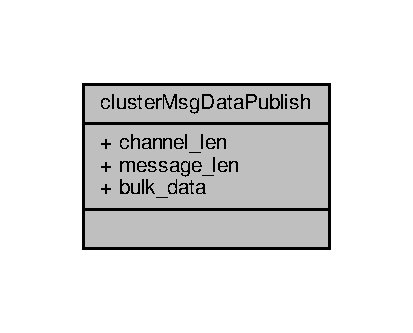
\includegraphics[width=198pt]{structclusterMsgDataPublish__coll__graph}
\end{center}
\end{figure}
\subsection*{Data Fields}
\begin{DoxyCompactItemize}
\item 
\mbox{\Hypertarget{structclusterMsgDataPublish_a278c4b7d83c96df2d56b7997e35daad3}\label{structclusterMsgDataPublish_a278c4b7d83c96df2d56b7997e35daad3}} 
uint32\+\_\+t {\bfseries channel\+\_\+len}
\item 
\mbox{\Hypertarget{structclusterMsgDataPublish_a409a267a5fe003303c9380ed3ff2f2e5}\label{structclusterMsgDataPublish_a409a267a5fe003303c9380ed3ff2f2e5}} 
uint32\+\_\+t {\bfseries message\+\_\+len}
\item 
\mbox{\Hypertarget{structclusterMsgDataPublish_a09627cf21fa82796a35abc80ab722afa}\label{structclusterMsgDataPublish_a09627cf21fa82796a35abc80ab722afa}} 
unsigned char {\bfseries bulk\+\_\+data} \mbox{[}8\mbox{]}
\end{DoxyCompactItemize}


\subsection{Detailed Description}


Definition at line \hyperlink{cluster_8h_source_l00192}{192} of file \hyperlink{cluster_8h_source}{cluster.\+h}.



\subsection{Field Documentation}
\mbox{\Hypertarget{structclusterMsgDataPublish_a09627cf21fa82796a35abc80ab722afa}\label{structclusterMsgDataPublish_a09627cf21fa82796a35abc80ab722afa}} 
\index{cluster\+Msg\+Data\+Publish@{cluster\+Msg\+Data\+Publish}!bulk\+\_\+data@{bulk\+\_\+data}}
\index{bulk\+\_\+data@{bulk\+\_\+data}!cluster\+Msg\+Data\+Publish@{cluster\+Msg\+Data\+Publish}}
\subsubsection{\texorpdfstring{bulk\+\_\+data}{bulk\_data}}
{\footnotesize\ttfamily unsigned char cluster\+Msg\+Data\+Publish\+::bulk\+\_\+data\mbox{[}8\mbox{]}}



Definition at line \hyperlink{cluster_8h_source_l00198}{198} of file \hyperlink{cluster_8h_source}{cluster.\+h}.

\mbox{\Hypertarget{structclusterMsgDataPublish_a278c4b7d83c96df2d56b7997e35daad3}\label{structclusterMsgDataPublish_a278c4b7d83c96df2d56b7997e35daad3}} 
\index{cluster\+Msg\+Data\+Publish@{cluster\+Msg\+Data\+Publish}!channel\+\_\+len@{channel\+\_\+len}}
\index{channel\+\_\+len@{channel\+\_\+len}!cluster\+Msg\+Data\+Publish@{cluster\+Msg\+Data\+Publish}}
\subsubsection{\texorpdfstring{channel\+\_\+len}{channel\_len}}
{\footnotesize\ttfamily uint32\+\_\+t cluster\+Msg\+Data\+Publish\+::channel\+\_\+len}



Definition at line \hyperlink{cluster_8h_source_l00193}{193} of file \hyperlink{cluster_8h_source}{cluster.\+h}.

\mbox{\Hypertarget{structclusterMsgDataPublish_a409a267a5fe003303c9380ed3ff2f2e5}\label{structclusterMsgDataPublish_a409a267a5fe003303c9380ed3ff2f2e5}} 
\index{cluster\+Msg\+Data\+Publish@{cluster\+Msg\+Data\+Publish}!message\+\_\+len@{message\+\_\+len}}
\index{message\+\_\+len@{message\+\_\+len}!cluster\+Msg\+Data\+Publish@{cluster\+Msg\+Data\+Publish}}
\subsubsection{\texorpdfstring{message\+\_\+len}{message\_len}}
{\footnotesize\ttfamily uint32\+\_\+t cluster\+Msg\+Data\+Publish\+::message\+\_\+len}



Definition at line \hyperlink{cluster_8h_source_l00194}{194} of file \hyperlink{cluster_8h_source}{cluster.\+h}.



The documentation for this struct was generated from the following file\+:\begin{DoxyCompactItemize}
\item 
src/cluster.\+h\end{DoxyCompactItemize}

\hypertarget{structclusterMsgDataUpdate}{}\section{cluster\+Msg\+Data\+Update Struct Reference}
\label{structclusterMsgDataUpdate}\index{cluster\+Msg\+Data\+Update@{cluster\+Msg\+Data\+Update}}


Collaboration diagram for cluster\+Msg\+Data\+Update\+:\nopagebreak
\begin{figure}[H]
\begin{center}
\leavevmode
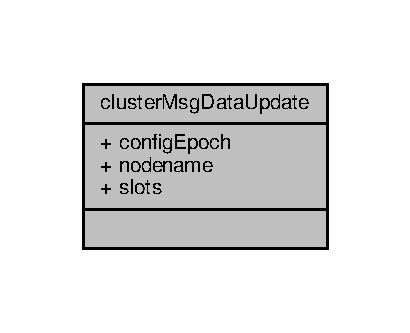
\includegraphics[width=197pt]{structclusterMsgDataUpdate__coll__graph}
\end{center}
\end{figure}
\subsection*{Data Fields}
\begin{DoxyCompactItemize}
\item 
\mbox{\Hypertarget{structclusterMsgDataUpdate_a5ccb48f1cbc2d86aa6665a3d91797fc5}\label{structclusterMsgDataUpdate_a5ccb48f1cbc2d86aa6665a3d91797fc5}} 
uint64\+\_\+t {\bfseries config\+Epoch}
\item 
\mbox{\Hypertarget{structclusterMsgDataUpdate_a506cd14d4ff4d1584e382b98abfed01d}\label{structclusterMsgDataUpdate_a506cd14d4ff4d1584e382b98abfed01d}} 
char {\bfseries nodename} \mbox{[}C\+L\+U\+S\+T\+E\+R\+\_\+\+N\+A\+M\+E\+L\+EN\mbox{]}
\item 
\mbox{\Hypertarget{structclusterMsgDataUpdate_ad644b488baff5a80184da68dd96234bb}\label{structclusterMsgDataUpdate_ad644b488baff5a80184da68dd96234bb}} 
unsigned char {\bfseries slots} \mbox{[}C\+L\+U\+S\+T\+E\+R\+\_\+\+S\+L\+O\+TS/8\mbox{]}
\end{DoxyCompactItemize}


\subsection{Detailed Description}


Definition at line \hyperlink{cluster_8h_source_l00201}{201} of file \hyperlink{cluster_8h_source}{cluster.\+h}.



\subsection{Field Documentation}
\mbox{\Hypertarget{structclusterMsgDataUpdate_a5ccb48f1cbc2d86aa6665a3d91797fc5}\label{structclusterMsgDataUpdate_a5ccb48f1cbc2d86aa6665a3d91797fc5}} 
\index{cluster\+Msg\+Data\+Update@{cluster\+Msg\+Data\+Update}!config\+Epoch@{config\+Epoch}}
\index{config\+Epoch@{config\+Epoch}!cluster\+Msg\+Data\+Update@{cluster\+Msg\+Data\+Update}}
\subsubsection{\texorpdfstring{config\+Epoch}{configEpoch}}
{\footnotesize\ttfamily uint64\+\_\+t cluster\+Msg\+Data\+Update\+::config\+Epoch}



Definition at line \hyperlink{cluster_8h_source_l00202}{202} of file \hyperlink{cluster_8h_source}{cluster.\+h}.

\mbox{\Hypertarget{structclusterMsgDataUpdate_a506cd14d4ff4d1584e382b98abfed01d}\label{structclusterMsgDataUpdate_a506cd14d4ff4d1584e382b98abfed01d}} 
\index{cluster\+Msg\+Data\+Update@{cluster\+Msg\+Data\+Update}!nodename@{nodename}}
\index{nodename@{nodename}!cluster\+Msg\+Data\+Update@{cluster\+Msg\+Data\+Update}}
\subsubsection{\texorpdfstring{nodename}{nodename}}
{\footnotesize\ttfamily char cluster\+Msg\+Data\+Update\+::nodename\mbox{[}C\+L\+U\+S\+T\+E\+R\+\_\+\+N\+A\+M\+E\+L\+EN\mbox{]}}



Definition at line \hyperlink{cluster_8h_source_l00203}{203} of file \hyperlink{cluster_8h_source}{cluster.\+h}.

\mbox{\Hypertarget{structclusterMsgDataUpdate_ad644b488baff5a80184da68dd96234bb}\label{structclusterMsgDataUpdate_ad644b488baff5a80184da68dd96234bb}} 
\index{cluster\+Msg\+Data\+Update@{cluster\+Msg\+Data\+Update}!slots@{slots}}
\index{slots@{slots}!cluster\+Msg\+Data\+Update@{cluster\+Msg\+Data\+Update}}
\subsubsection{\texorpdfstring{slots}{slots}}
{\footnotesize\ttfamily unsigned char cluster\+Msg\+Data\+Update\+::slots\mbox{[}C\+L\+U\+S\+T\+E\+R\+\_\+\+S\+L\+O\+TS/8\mbox{]}}



Definition at line \hyperlink{cluster_8h_source_l00204}{204} of file \hyperlink{cluster_8h_source}{cluster.\+h}.



The documentation for this struct was generated from the following file\+:\begin{DoxyCompactItemize}
\item 
src/cluster.\+h\end{DoxyCompactItemize}

\hypertarget{structclusterNode}{}\section{cluster\+Node Struct Reference}
\label{structclusterNode}\index{cluster\+Node@{cluster\+Node}}


Collaboration diagram for cluster\+Node\+:\nopagebreak
\begin{figure}[H]
\begin{center}
\leavevmode
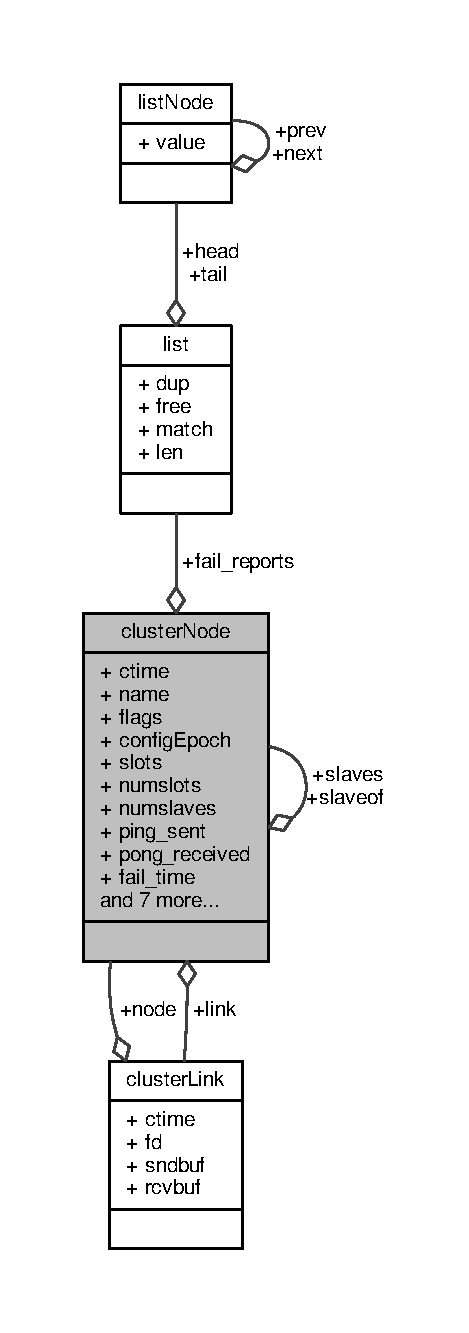
\includegraphics[height=550pt]{structclusterNode__coll__graph}
\end{center}
\end{figure}
\subsection*{Data Fields}
\begin{DoxyCompactItemize}
\item 
\mbox{\Hypertarget{structclusterNode_aa33a6402dfdda11c2b84272b262ee945}\label{structclusterNode_aa33a6402dfdda11c2b84272b262ee945}} 
mstime\+\_\+t {\bfseries ctime}
\item 
\mbox{\Hypertarget{structclusterNode_ae0214470697f2a171d6cdd3493facbb2}\label{structclusterNode_ae0214470697f2a171d6cdd3493facbb2}} 
char {\bfseries name} \mbox{[}C\+L\+U\+S\+T\+E\+R\+\_\+\+N\+A\+M\+E\+L\+EN\mbox{]}
\item 
\mbox{\Hypertarget{structclusterNode_a496b52bc0e6536e9556c6eb2779c03eb}\label{structclusterNode_a496b52bc0e6536e9556c6eb2779c03eb}} 
int {\bfseries flags}
\item 
\mbox{\Hypertarget{structclusterNode_aa72bc6455e36e662bc5a53fc427452a5}\label{structclusterNode_aa72bc6455e36e662bc5a53fc427452a5}} 
uint64\+\_\+t {\bfseries config\+Epoch}
\item 
\mbox{\Hypertarget{structclusterNode_a8c8302e4633d2d0094fa621ecfcf1b52}\label{structclusterNode_a8c8302e4633d2d0094fa621ecfcf1b52}} 
unsigned char {\bfseries slots} \mbox{[}C\+L\+U\+S\+T\+E\+R\+\_\+\+S\+L\+O\+TS/8\mbox{]}
\item 
\mbox{\Hypertarget{structclusterNode_a369c3823027d5aef6928189b480f52ee}\label{structclusterNode_a369c3823027d5aef6928189b480f52ee}} 
int {\bfseries numslots}
\item 
\mbox{\Hypertarget{structclusterNode_a7e3b31fb7e833940d50a5a7d7d1f148d}\label{structclusterNode_a7e3b31fb7e833940d50a5a7d7d1f148d}} 
int {\bfseries numslaves}
\item 
\mbox{\Hypertarget{structclusterNode_a35eac3f31a0acdbb1cf8d20fff406da6}\label{structclusterNode_a35eac3f31a0acdbb1cf8d20fff406da6}} 
struct \hyperlink{structclusterNode}{cluster\+Node} $\ast$$\ast$ {\bfseries slaves}
\item 
\mbox{\Hypertarget{structclusterNode_aabb2536cdf382cec6d810aaf0ba9f58a}\label{structclusterNode_aabb2536cdf382cec6d810aaf0ba9f58a}} 
struct \hyperlink{structclusterNode}{cluster\+Node} $\ast$ {\bfseries slaveof}
\item 
\mbox{\Hypertarget{structclusterNode_ab3eb79015f20bf51dc971da964133f0b}\label{structclusterNode_ab3eb79015f20bf51dc971da964133f0b}} 
mstime\+\_\+t {\bfseries ping\+\_\+sent}
\item 
\mbox{\Hypertarget{structclusterNode_a58e3914e6485d5fcba3b14d28ef053e8}\label{structclusterNode_a58e3914e6485d5fcba3b14d28ef053e8}} 
mstime\+\_\+t {\bfseries pong\+\_\+received}
\item 
\mbox{\Hypertarget{structclusterNode_ab2aa62006e87ba83e3139b9d28c6eb18}\label{structclusterNode_ab2aa62006e87ba83e3139b9d28c6eb18}} 
mstime\+\_\+t {\bfseries fail\+\_\+time}
\item 
\mbox{\Hypertarget{structclusterNode_a871c18dd4ac7662af3e8fc3c699ece81}\label{structclusterNode_a871c18dd4ac7662af3e8fc3c699ece81}} 
mstime\+\_\+t {\bfseries voted\+\_\+time}
\item 
\mbox{\Hypertarget{structclusterNode_a025057023f653785bb08de23072553d2}\label{structclusterNode_a025057023f653785bb08de23072553d2}} 
mstime\+\_\+t {\bfseries repl\+\_\+offset\+\_\+time}
\item 
\mbox{\Hypertarget{structclusterNode_a70a653ebe05b396d234db25b51bffeb6}\label{structclusterNode_a70a653ebe05b396d234db25b51bffeb6}} 
mstime\+\_\+t {\bfseries orphaned\+\_\+time}
\item 
\mbox{\Hypertarget{structclusterNode_a71e240137314f16e9b6bd3baa2075ef8}\label{structclusterNode_a71e240137314f16e9b6bd3baa2075ef8}} 
long long {\bfseries repl\+\_\+offset}
\item 
\mbox{\Hypertarget{structclusterNode_af5fe551fd3955ee170ac36422e6637f2}\label{structclusterNode_af5fe551fd3955ee170ac36422e6637f2}} 
char {\bfseries ip} \mbox{[}N\+E\+T\+\_\+\+I\+P\+\_\+\+S\+T\+R\+\_\+\+L\+EN\mbox{]}
\item 
\mbox{\Hypertarget{structclusterNode_a8625d7d4a94bdab4579d3289850f17d1}\label{structclusterNode_a8625d7d4a94bdab4579d3289850f17d1}} 
int {\bfseries port}
\item 
\mbox{\Hypertarget{structclusterNode_afd795cbf257e028b15baa5338ebf10e8}\label{structclusterNode_afd795cbf257e028b15baa5338ebf10e8}} 
int {\bfseries cport}
\item 
\mbox{\Hypertarget{structclusterNode_a2a132086324ba85e15a911b9bd5ef94b}\label{structclusterNode_a2a132086324ba85e15a911b9bd5ef94b}} 
\hyperlink{structclusterLink}{cluster\+Link} $\ast$ {\bfseries link}
\item 
\mbox{\Hypertarget{structclusterNode_ab683b7bff2f7ea87a9f42def23e8400f}\label{structclusterNode_ab683b7bff2f7ea87a9f42def23e8400f}} 
\hyperlink{structlist}{list} $\ast$ {\bfseries fail\+\_\+reports}
\end{DoxyCompactItemize}


\subsection{Detailed Description}


Definition at line \hyperlink{cluster_8h_source_l00105}{105} of file \hyperlink{cluster_8h_source}{cluster.\+h}.



\subsection{Field Documentation}
\mbox{\Hypertarget{structclusterNode_aa72bc6455e36e662bc5a53fc427452a5}\label{structclusterNode_aa72bc6455e36e662bc5a53fc427452a5}} 
\index{cluster\+Node@{cluster\+Node}!config\+Epoch@{config\+Epoch}}
\index{config\+Epoch@{config\+Epoch}!cluster\+Node@{cluster\+Node}}
\subsubsection{\texorpdfstring{config\+Epoch}{configEpoch}}
{\footnotesize\ttfamily uint64\+\_\+t cluster\+Node\+::config\+Epoch}



Definition at line \hyperlink{cluster_8h_source_l00109}{109} of file \hyperlink{cluster_8h_source}{cluster.\+h}.

\mbox{\Hypertarget{structclusterNode_afd795cbf257e028b15baa5338ebf10e8}\label{structclusterNode_afd795cbf257e028b15baa5338ebf10e8}} 
\index{cluster\+Node@{cluster\+Node}!cport@{cport}}
\index{cport@{cport}!cluster\+Node@{cluster\+Node}}
\subsubsection{\texorpdfstring{cport}{cport}}
{\footnotesize\ttfamily int cluster\+Node\+::cport}



Definition at line \hyperlink{cluster_8h_source_l00127}{127} of file \hyperlink{cluster_8h_source}{cluster.\+h}.

\mbox{\Hypertarget{structclusterNode_aa33a6402dfdda11c2b84272b262ee945}\label{structclusterNode_aa33a6402dfdda11c2b84272b262ee945}} 
\index{cluster\+Node@{cluster\+Node}!ctime@{ctime}}
\index{ctime@{ctime}!cluster\+Node@{cluster\+Node}}
\subsubsection{\texorpdfstring{ctime}{ctime}}
{\footnotesize\ttfamily mstime\+\_\+t cluster\+Node\+::ctime}



Definition at line \hyperlink{cluster_8h_source_l00106}{106} of file \hyperlink{cluster_8h_source}{cluster.\+h}.

\mbox{\Hypertarget{structclusterNode_ab683b7bff2f7ea87a9f42def23e8400f}\label{structclusterNode_ab683b7bff2f7ea87a9f42def23e8400f}} 
\index{cluster\+Node@{cluster\+Node}!fail\+\_\+reports@{fail\+\_\+reports}}
\index{fail\+\_\+reports@{fail\+\_\+reports}!cluster\+Node@{cluster\+Node}}
\subsubsection{\texorpdfstring{fail\+\_\+reports}{fail\_reports}}
{\footnotesize\ttfamily \hyperlink{structlist}{list}$\ast$ cluster\+Node\+::fail\+\_\+reports}



Definition at line \hyperlink{cluster_8h_source_l00129}{129} of file \hyperlink{cluster_8h_source}{cluster.\+h}.

\mbox{\Hypertarget{structclusterNode_ab2aa62006e87ba83e3139b9d28c6eb18}\label{structclusterNode_ab2aa62006e87ba83e3139b9d28c6eb18}} 
\index{cluster\+Node@{cluster\+Node}!fail\+\_\+time@{fail\+\_\+time}}
\index{fail\+\_\+time@{fail\+\_\+time}!cluster\+Node@{cluster\+Node}}
\subsubsection{\texorpdfstring{fail\+\_\+time}{fail\_time}}
{\footnotesize\ttfamily mstime\+\_\+t cluster\+Node\+::fail\+\_\+time}



Definition at line \hyperlink{cluster_8h_source_l00120}{120} of file \hyperlink{cluster_8h_source}{cluster.\+h}.

\mbox{\Hypertarget{structclusterNode_a496b52bc0e6536e9556c6eb2779c03eb}\label{structclusterNode_a496b52bc0e6536e9556c6eb2779c03eb}} 
\index{cluster\+Node@{cluster\+Node}!flags@{flags}}
\index{flags@{flags}!cluster\+Node@{cluster\+Node}}
\subsubsection{\texorpdfstring{flags}{flags}}
{\footnotesize\ttfamily int cluster\+Node\+::flags}



Definition at line \hyperlink{cluster_8h_source_l00108}{108} of file \hyperlink{cluster_8h_source}{cluster.\+h}.

\mbox{\Hypertarget{structclusterNode_af5fe551fd3955ee170ac36422e6637f2}\label{structclusterNode_af5fe551fd3955ee170ac36422e6637f2}} 
\index{cluster\+Node@{cluster\+Node}!ip@{ip}}
\index{ip@{ip}!cluster\+Node@{cluster\+Node}}
\subsubsection{\texorpdfstring{ip}{ip}}
{\footnotesize\ttfamily char cluster\+Node\+::ip\mbox{[}N\+E\+T\+\_\+\+I\+P\+\_\+\+S\+T\+R\+\_\+\+L\+EN\mbox{]}}



Definition at line \hyperlink{cluster_8h_source_l00125}{125} of file \hyperlink{cluster_8h_source}{cluster.\+h}.

\mbox{\Hypertarget{structclusterNode_a2a132086324ba85e15a911b9bd5ef94b}\label{structclusterNode_a2a132086324ba85e15a911b9bd5ef94b}} 
\index{cluster\+Node@{cluster\+Node}!link@{link}}
\index{link@{link}!cluster\+Node@{cluster\+Node}}
\subsubsection{\texorpdfstring{link}{link}}
{\footnotesize\ttfamily \hyperlink{structclusterLink}{cluster\+Link}$\ast$ cluster\+Node\+::link}



Definition at line \hyperlink{cluster_8h_source_l00128}{128} of file \hyperlink{cluster_8h_source}{cluster.\+h}.

\mbox{\Hypertarget{structclusterNode_ae0214470697f2a171d6cdd3493facbb2}\label{structclusterNode_ae0214470697f2a171d6cdd3493facbb2}} 
\index{cluster\+Node@{cluster\+Node}!name@{name}}
\index{name@{name}!cluster\+Node@{cluster\+Node}}
\subsubsection{\texorpdfstring{name}{name}}
{\footnotesize\ttfamily char cluster\+Node\+::name\mbox{[}C\+L\+U\+S\+T\+E\+R\+\_\+\+N\+A\+M\+E\+L\+EN\mbox{]}}



Definition at line \hyperlink{cluster_8h_source_l00107}{107} of file \hyperlink{cluster_8h_source}{cluster.\+h}.

\mbox{\Hypertarget{structclusterNode_a7e3b31fb7e833940d50a5a7d7d1f148d}\label{structclusterNode_a7e3b31fb7e833940d50a5a7d7d1f148d}} 
\index{cluster\+Node@{cluster\+Node}!numslaves@{numslaves}}
\index{numslaves@{numslaves}!cluster\+Node@{cluster\+Node}}
\subsubsection{\texorpdfstring{numslaves}{numslaves}}
{\footnotesize\ttfamily int cluster\+Node\+::numslaves}



Definition at line \hyperlink{cluster_8h_source_l00112}{112} of file \hyperlink{cluster_8h_source}{cluster.\+h}.

\mbox{\Hypertarget{structclusterNode_a369c3823027d5aef6928189b480f52ee}\label{structclusterNode_a369c3823027d5aef6928189b480f52ee}} 
\index{cluster\+Node@{cluster\+Node}!numslots@{numslots}}
\index{numslots@{numslots}!cluster\+Node@{cluster\+Node}}
\subsubsection{\texorpdfstring{numslots}{numslots}}
{\footnotesize\ttfamily int cluster\+Node\+::numslots}



Definition at line \hyperlink{cluster_8h_source_l00111}{111} of file \hyperlink{cluster_8h_source}{cluster.\+h}.

\mbox{\Hypertarget{structclusterNode_a70a653ebe05b396d234db25b51bffeb6}\label{structclusterNode_a70a653ebe05b396d234db25b51bffeb6}} 
\index{cluster\+Node@{cluster\+Node}!orphaned\+\_\+time@{orphaned\+\_\+time}}
\index{orphaned\+\_\+time@{orphaned\+\_\+time}!cluster\+Node@{cluster\+Node}}
\subsubsection{\texorpdfstring{orphaned\+\_\+time}{orphaned\_time}}
{\footnotesize\ttfamily mstime\+\_\+t cluster\+Node\+::orphaned\+\_\+time}



Definition at line \hyperlink{cluster_8h_source_l00123}{123} of file \hyperlink{cluster_8h_source}{cluster.\+h}.

\mbox{\Hypertarget{structclusterNode_ab3eb79015f20bf51dc971da964133f0b}\label{structclusterNode_ab3eb79015f20bf51dc971da964133f0b}} 
\index{cluster\+Node@{cluster\+Node}!ping\+\_\+sent@{ping\+\_\+sent}}
\index{ping\+\_\+sent@{ping\+\_\+sent}!cluster\+Node@{cluster\+Node}}
\subsubsection{\texorpdfstring{ping\+\_\+sent}{ping\_sent}}
{\footnotesize\ttfamily mstime\+\_\+t cluster\+Node\+::ping\+\_\+sent}



Definition at line \hyperlink{cluster_8h_source_l00118}{118} of file \hyperlink{cluster_8h_source}{cluster.\+h}.

\mbox{\Hypertarget{structclusterNode_a58e3914e6485d5fcba3b14d28ef053e8}\label{structclusterNode_a58e3914e6485d5fcba3b14d28ef053e8}} 
\index{cluster\+Node@{cluster\+Node}!pong\+\_\+received@{pong\+\_\+received}}
\index{pong\+\_\+received@{pong\+\_\+received}!cluster\+Node@{cluster\+Node}}
\subsubsection{\texorpdfstring{pong\+\_\+received}{pong\_received}}
{\footnotesize\ttfamily mstime\+\_\+t cluster\+Node\+::pong\+\_\+received}



Definition at line \hyperlink{cluster_8h_source_l00119}{119} of file \hyperlink{cluster_8h_source}{cluster.\+h}.

\mbox{\Hypertarget{structclusterNode_a8625d7d4a94bdab4579d3289850f17d1}\label{structclusterNode_a8625d7d4a94bdab4579d3289850f17d1}} 
\index{cluster\+Node@{cluster\+Node}!port@{port}}
\index{port@{port}!cluster\+Node@{cluster\+Node}}
\subsubsection{\texorpdfstring{port}{port}}
{\footnotesize\ttfamily int cluster\+Node\+::port}



Definition at line \hyperlink{cluster_8h_source_l00126}{126} of file \hyperlink{cluster_8h_source}{cluster.\+h}.

\mbox{\Hypertarget{structclusterNode_a71e240137314f16e9b6bd3baa2075ef8}\label{structclusterNode_a71e240137314f16e9b6bd3baa2075ef8}} 
\index{cluster\+Node@{cluster\+Node}!repl\+\_\+offset@{repl\+\_\+offset}}
\index{repl\+\_\+offset@{repl\+\_\+offset}!cluster\+Node@{cluster\+Node}}
\subsubsection{\texorpdfstring{repl\+\_\+offset}{repl\_offset}}
{\footnotesize\ttfamily long long cluster\+Node\+::repl\+\_\+offset}



Definition at line \hyperlink{cluster_8h_source_l00124}{124} of file \hyperlink{cluster_8h_source}{cluster.\+h}.

\mbox{\Hypertarget{structclusterNode_a025057023f653785bb08de23072553d2}\label{structclusterNode_a025057023f653785bb08de23072553d2}} 
\index{cluster\+Node@{cluster\+Node}!repl\+\_\+offset\+\_\+time@{repl\+\_\+offset\+\_\+time}}
\index{repl\+\_\+offset\+\_\+time@{repl\+\_\+offset\+\_\+time}!cluster\+Node@{cluster\+Node}}
\subsubsection{\texorpdfstring{repl\+\_\+offset\+\_\+time}{repl\_offset\_time}}
{\footnotesize\ttfamily mstime\+\_\+t cluster\+Node\+::repl\+\_\+offset\+\_\+time}



Definition at line \hyperlink{cluster_8h_source_l00122}{122} of file \hyperlink{cluster_8h_source}{cluster.\+h}.

\mbox{\Hypertarget{structclusterNode_aabb2536cdf382cec6d810aaf0ba9f58a}\label{structclusterNode_aabb2536cdf382cec6d810aaf0ba9f58a}} 
\index{cluster\+Node@{cluster\+Node}!slaveof@{slaveof}}
\index{slaveof@{slaveof}!cluster\+Node@{cluster\+Node}}
\subsubsection{\texorpdfstring{slaveof}{slaveof}}
{\footnotesize\ttfamily struct \hyperlink{structclusterNode}{cluster\+Node}$\ast$ cluster\+Node\+::slaveof}



Definition at line \hyperlink{cluster_8h_source_l00114}{114} of file \hyperlink{cluster_8h_source}{cluster.\+h}.

\mbox{\Hypertarget{structclusterNode_a35eac3f31a0acdbb1cf8d20fff406da6}\label{structclusterNode_a35eac3f31a0acdbb1cf8d20fff406da6}} 
\index{cluster\+Node@{cluster\+Node}!slaves@{slaves}}
\index{slaves@{slaves}!cluster\+Node@{cluster\+Node}}
\subsubsection{\texorpdfstring{slaves}{slaves}}
{\footnotesize\ttfamily struct \hyperlink{structclusterNode}{cluster\+Node}$\ast$$\ast$ cluster\+Node\+::slaves}



Definition at line \hyperlink{cluster_8h_source_l00113}{113} of file \hyperlink{cluster_8h_source}{cluster.\+h}.

\mbox{\Hypertarget{structclusterNode_a8c8302e4633d2d0094fa621ecfcf1b52}\label{structclusterNode_a8c8302e4633d2d0094fa621ecfcf1b52}} 
\index{cluster\+Node@{cluster\+Node}!slots@{slots}}
\index{slots@{slots}!cluster\+Node@{cluster\+Node}}
\subsubsection{\texorpdfstring{slots}{slots}}
{\footnotesize\ttfamily unsigned char cluster\+Node\+::slots\mbox{[}C\+L\+U\+S\+T\+E\+R\+\_\+\+S\+L\+O\+TS/8\mbox{]}}



Definition at line \hyperlink{cluster_8h_source_l00110}{110} of file \hyperlink{cluster_8h_source}{cluster.\+h}.

\mbox{\Hypertarget{structclusterNode_a871c18dd4ac7662af3e8fc3c699ece81}\label{structclusterNode_a871c18dd4ac7662af3e8fc3c699ece81}} 
\index{cluster\+Node@{cluster\+Node}!voted\+\_\+time@{voted\+\_\+time}}
\index{voted\+\_\+time@{voted\+\_\+time}!cluster\+Node@{cluster\+Node}}
\subsubsection{\texorpdfstring{voted\+\_\+time}{voted\_time}}
{\footnotesize\ttfamily mstime\+\_\+t cluster\+Node\+::voted\+\_\+time}



Definition at line \hyperlink{cluster_8h_source_l00121}{121} of file \hyperlink{cluster_8h_source}{cluster.\+h}.



The documentation for this struct was generated from the following file\+:\begin{DoxyCompactItemize}
\item 
src/cluster.\+h\end{DoxyCompactItemize}

\hypertarget{structclusterNodeFailReport}{}\section{cluster\+Node\+Fail\+Report Struct Reference}
\label{structclusterNodeFailReport}\index{cluster\+Node\+Fail\+Report@{cluster\+Node\+Fail\+Report}}


Collaboration diagram for cluster\+Node\+Fail\+Report\+:\nopagebreak
\begin{figure}[H]
\begin{center}
\leavevmode
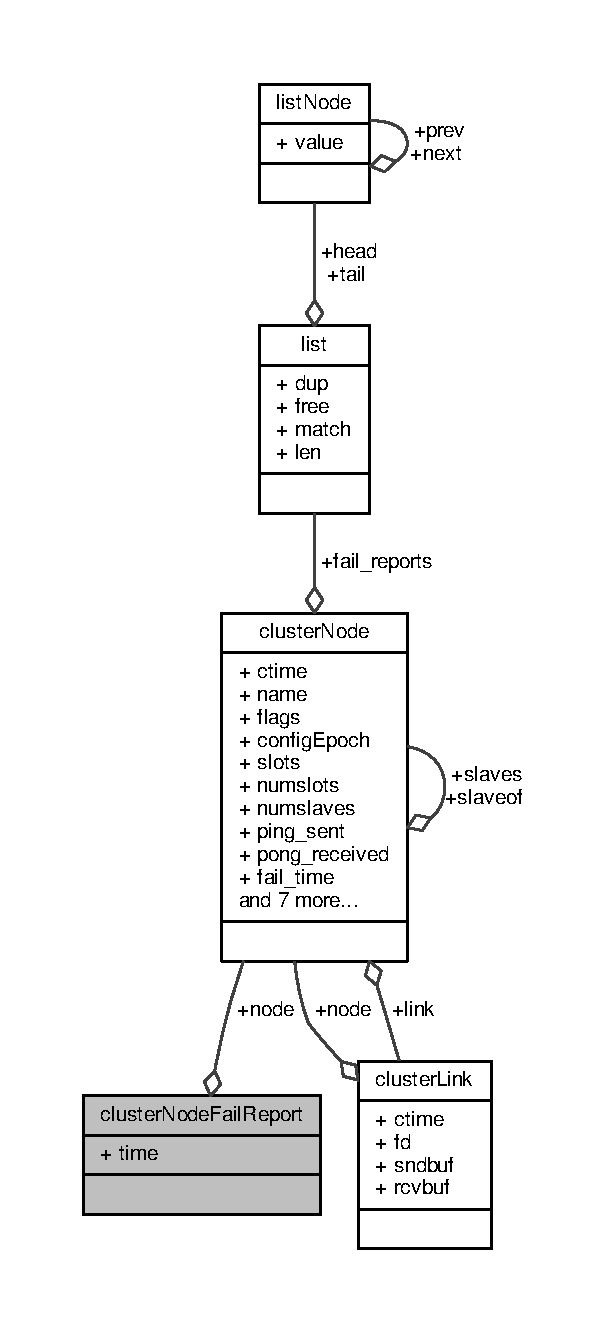
\includegraphics[height=550pt]{structclusterNodeFailReport__coll__graph}
\end{center}
\end{figure}
\subsection*{Data Fields}
\begin{DoxyCompactItemize}
\item 
\mbox{\Hypertarget{structclusterNodeFailReport_ad6b6931afca6e6d732ef32adcbd93585}\label{structclusterNodeFailReport_ad6b6931afca6e6d732ef32adcbd93585}} 
struct \hyperlink{structclusterNode}{cluster\+Node} $\ast$ {\bfseries node}
\item 
\mbox{\Hypertarget{structclusterNodeFailReport_ae635d169cc9256b72c5cb8e6beb3d873}\label{structclusterNodeFailReport_ae635d169cc9256b72c5cb8e6beb3d873}} 
mstime\+\_\+t {\bfseries time}
\end{DoxyCompactItemize}


\subsection{Detailed Description}


Definition at line \hyperlink{cluster_8h_source_l00100}{100} of file \hyperlink{cluster_8h_source}{cluster.\+h}.



\subsection{Field Documentation}
\mbox{\Hypertarget{structclusterNodeFailReport_ad6b6931afca6e6d732ef32adcbd93585}\label{structclusterNodeFailReport_ad6b6931afca6e6d732ef32adcbd93585}} 
\index{cluster\+Node\+Fail\+Report@{cluster\+Node\+Fail\+Report}!node@{node}}
\index{node@{node}!cluster\+Node\+Fail\+Report@{cluster\+Node\+Fail\+Report}}
\subsubsection{\texorpdfstring{node}{node}}
{\footnotesize\ttfamily struct \hyperlink{structclusterNode}{cluster\+Node}$\ast$ cluster\+Node\+Fail\+Report\+::node}



Definition at line \hyperlink{cluster_8h_source_l00101}{101} of file \hyperlink{cluster_8h_source}{cluster.\+h}.

\mbox{\Hypertarget{structclusterNodeFailReport_ae635d169cc9256b72c5cb8e6beb3d873}\label{structclusterNodeFailReport_ae635d169cc9256b72c5cb8e6beb3d873}} 
\index{cluster\+Node\+Fail\+Report@{cluster\+Node\+Fail\+Report}!time@{time}}
\index{time@{time}!cluster\+Node\+Fail\+Report@{cluster\+Node\+Fail\+Report}}
\subsubsection{\texorpdfstring{time}{time}}
{\footnotesize\ttfamily mstime\+\_\+t cluster\+Node\+Fail\+Report\+::time}



Definition at line \hyperlink{cluster_8h_source_l00102}{102} of file \hyperlink{cluster_8h_source}{cluster.\+h}.



The documentation for this struct was generated from the following file\+:\begin{DoxyCompactItemize}
\item 
src/cluster.\+h\end{DoxyCompactItemize}

\hypertarget{structclusterState}{}\section{cluster\+State Struct Reference}
\label{structclusterState}\index{cluster\+State@{cluster\+State}}


Collaboration diagram for cluster\+State\+:\nopagebreak
\begin{figure}[H]
\begin{center}
\leavevmode
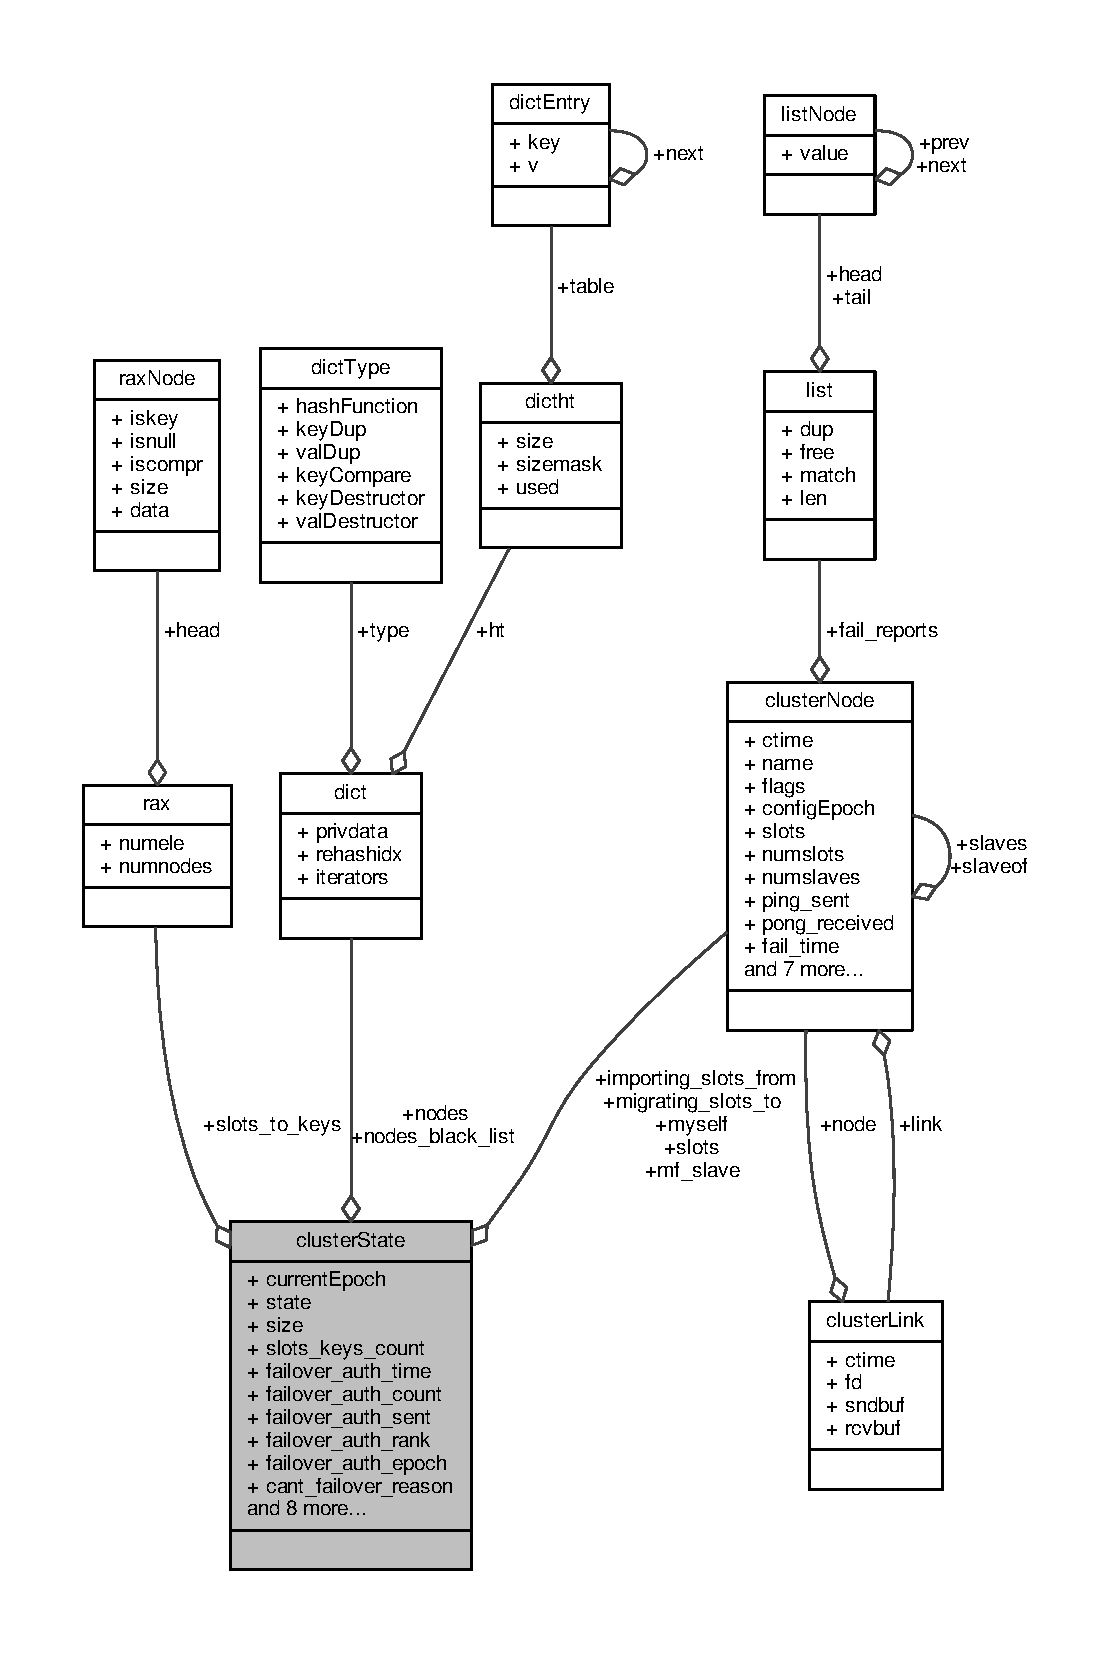
\includegraphics[width=350pt]{structclusterState__coll__graph}
\end{center}
\end{figure}
\subsection*{Data Fields}
\begin{DoxyCompactItemize}
\item 
\mbox{\Hypertarget{structclusterState_a40512f248f0162974ee06af5a1ab3d0c}\label{structclusterState_a40512f248f0162974ee06af5a1ab3d0c}} 
\hyperlink{structclusterNode}{cluster\+Node} $\ast$ {\bfseries myself}
\item 
\mbox{\Hypertarget{structclusterState_a5119e8f4572f08816e666b1a078ba63c}\label{structclusterState_a5119e8f4572f08816e666b1a078ba63c}} 
uint64\+\_\+t {\bfseries current\+Epoch}
\item 
\mbox{\Hypertarget{structclusterState_a21aad7dbd75931914c80348cb00ae37b}\label{structclusterState_a21aad7dbd75931914c80348cb00ae37b}} 
int {\bfseries state}
\item 
\mbox{\Hypertarget{structclusterState_ac412fd88c5d16098266b34a8ca983906}\label{structclusterState_ac412fd88c5d16098266b34a8ca983906}} 
int {\bfseries size}
\item 
\mbox{\Hypertarget{structclusterState_aa931d12287ceee735a18a2bbf22575fb}\label{structclusterState_aa931d12287ceee735a18a2bbf22575fb}} 
\hyperlink{structdict}{dict} $\ast$ {\bfseries nodes}
\item 
\mbox{\Hypertarget{structclusterState_af1282691ef30aad603edaf8573864364}\label{structclusterState_af1282691ef30aad603edaf8573864364}} 
\hyperlink{structdict}{dict} $\ast$ {\bfseries nodes\+\_\+black\+\_\+list}
\item 
\mbox{\Hypertarget{structclusterState_ac79d09770ee5089effad9ba6b60d8ea7}\label{structclusterState_ac79d09770ee5089effad9ba6b60d8ea7}} 
\hyperlink{structclusterNode}{cluster\+Node} $\ast$ {\bfseries migrating\+\_\+slots\+\_\+to} \mbox{[}C\+L\+U\+S\+T\+E\+R\+\_\+\+S\+L\+O\+TS\mbox{]}
\item 
\mbox{\Hypertarget{structclusterState_a63639e9efbfdc877fa58a42d5609e49a}\label{structclusterState_a63639e9efbfdc877fa58a42d5609e49a}} 
\hyperlink{structclusterNode}{cluster\+Node} $\ast$ {\bfseries importing\+\_\+slots\+\_\+from} \mbox{[}C\+L\+U\+S\+T\+E\+R\+\_\+\+S\+L\+O\+TS\mbox{]}
\item 
\mbox{\Hypertarget{structclusterState_a3cb4d898f159addb27ef10d737d77842}\label{structclusterState_a3cb4d898f159addb27ef10d737d77842}} 
\hyperlink{structclusterNode}{cluster\+Node} $\ast$ {\bfseries slots} \mbox{[}C\+L\+U\+S\+T\+E\+R\+\_\+\+S\+L\+O\+TS\mbox{]}
\item 
\mbox{\Hypertarget{structclusterState_ae85ad11c2ebc8a680883bf2e14a930d8}\label{structclusterState_ae85ad11c2ebc8a680883bf2e14a930d8}} 
uint64\+\_\+t {\bfseries slots\+\_\+keys\+\_\+count} \mbox{[}C\+L\+U\+S\+T\+E\+R\+\_\+\+S\+L\+O\+TS\mbox{]}
\item 
\mbox{\Hypertarget{structclusterState_a75096139a10c1d93a9aa39e0127767c6}\label{structclusterState_a75096139a10c1d93a9aa39e0127767c6}} 
\hyperlink{structrax}{rax} $\ast$ {\bfseries slots\+\_\+to\+\_\+keys}
\item 
\mbox{\Hypertarget{structclusterState_ae4ecf61e881a8d51e08b0737c3ced2dc}\label{structclusterState_ae4ecf61e881a8d51e08b0737c3ced2dc}} 
mstime\+\_\+t {\bfseries failover\+\_\+auth\+\_\+time}
\item 
\mbox{\Hypertarget{structclusterState_a680bfceed44d08476cabfb4ff69e406c}\label{structclusterState_a680bfceed44d08476cabfb4ff69e406c}} 
int {\bfseries failover\+\_\+auth\+\_\+count}
\item 
\mbox{\Hypertarget{structclusterState_a3b6d9abb6c5bd0cd96ebf8478d9dacdd}\label{structclusterState_a3b6d9abb6c5bd0cd96ebf8478d9dacdd}} 
int {\bfseries failover\+\_\+auth\+\_\+sent}
\item 
\mbox{\Hypertarget{structclusterState_a04b0fcfbf51ba160dfaa92e3009b8cb1}\label{structclusterState_a04b0fcfbf51ba160dfaa92e3009b8cb1}} 
int {\bfseries failover\+\_\+auth\+\_\+rank}
\item 
\mbox{\Hypertarget{structclusterState_a0b155aa7170d100f391bceb01660813d}\label{structclusterState_a0b155aa7170d100f391bceb01660813d}} 
uint64\+\_\+t {\bfseries failover\+\_\+auth\+\_\+epoch}
\item 
\mbox{\Hypertarget{structclusterState_a1a1d4314d9283a63d2c9167d6560f130}\label{structclusterState_a1a1d4314d9283a63d2c9167d6560f130}} 
int {\bfseries cant\+\_\+failover\+\_\+reason}
\item 
\mbox{\Hypertarget{structclusterState_af3ea36bbd489586bc9fcd1a006657f72}\label{structclusterState_af3ea36bbd489586bc9fcd1a006657f72}} 
mstime\+\_\+t {\bfseries mf\+\_\+end}
\item 
\mbox{\Hypertarget{structclusterState_aa5e779b422ba935a084af8242ee7526a}\label{structclusterState_aa5e779b422ba935a084af8242ee7526a}} 
\hyperlink{structclusterNode}{cluster\+Node} $\ast$ {\bfseries mf\+\_\+slave}
\item 
\mbox{\Hypertarget{structclusterState_ad5b4da4752c6da732602b3dd858a9977}\label{structclusterState_ad5b4da4752c6da732602b3dd858a9977}} 
long long {\bfseries mf\+\_\+master\+\_\+offset}
\item 
\mbox{\Hypertarget{structclusterState_a936611435312046bab0e1606ff815528}\label{structclusterState_a936611435312046bab0e1606ff815528}} 
int {\bfseries mf\+\_\+can\+\_\+start}
\item 
\mbox{\Hypertarget{structclusterState_a94332a392b06214e98b82e5470fbff86}\label{structclusterState_a94332a392b06214e98b82e5470fbff86}} 
uint64\+\_\+t {\bfseries last\+Vote\+Epoch}
\item 
\mbox{\Hypertarget{structclusterState_ac9c16c374097b11583e5660659e2bc7a}\label{structclusterState_ac9c16c374097b11583e5660659e2bc7a}} 
int {\bfseries todo\+\_\+before\+\_\+sleep}
\item 
\mbox{\Hypertarget{structclusterState_a2e05a3efe6eef76b7db90b03f8a71a50}\label{structclusterState_a2e05a3efe6eef76b7db90b03f8a71a50}} 
long long {\bfseries stats\+\_\+bus\+\_\+messages\+\_\+sent} \mbox{[}C\+L\+U\+S\+T\+E\+R\+M\+S\+G\+\_\+\+T\+Y\+P\+E\+\_\+\+C\+O\+U\+NT\mbox{]}
\item 
\mbox{\Hypertarget{structclusterState_ada00674128868894d7b81a5bcadf6994}\label{structclusterState_ada00674128868894d7b81a5bcadf6994}} 
long long {\bfseries stats\+\_\+bus\+\_\+messages\+\_\+received} \mbox{[}C\+L\+U\+S\+T\+E\+R\+M\+S\+G\+\_\+\+T\+Y\+P\+E\+\_\+\+C\+O\+U\+NT\mbox{]}
\item 
\mbox{\Hypertarget{structclusterState_ab6b2341a5c8bb775387a45c350c4a335}\label{structclusterState_ab6b2341a5c8bb775387a45c350c4a335}} 
long long {\bfseries stats\+\_\+pfail\+\_\+nodes}
\end{DoxyCompactItemize}


\subsection{Detailed Description}


Definition at line \hyperlink{cluster_8h_source_l00132}{132} of file \hyperlink{cluster_8h_source}{cluster.\+h}.



\subsection{Field Documentation}
\mbox{\Hypertarget{structclusterState_a1a1d4314d9283a63d2c9167d6560f130}\label{structclusterState_a1a1d4314d9283a63d2c9167d6560f130}} 
\index{cluster\+State@{cluster\+State}!cant\+\_\+failover\+\_\+reason@{cant\+\_\+failover\+\_\+reason}}
\index{cant\+\_\+failover\+\_\+reason@{cant\+\_\+failover\+\_\+reason}!cluster\+State@{cluster\+State}}
\subsubsection{\texorpdfstring{cant\+\_\+failover\+\_\+reason}{cant\_failover\_reason}}
{\footnotesize\ttfamily int cluster\+State\+::cant\+\_\+failover\+\_\+reason}



Definition at line \hyperlink{cluster_8h_source_l00150}{150} of file \hyperlink{cluster_8h_source}{cluster.\+h}.

\mbox{\Hypertarget{structclusterState_a5119e8f4572f08816e666b1a078ba63c}\label{structclusterState_a5119e8f4572f08816e666b1a078ba63c}} 
\index{cluster\+State@{cluster\+State}!current\+Epoch@{current\+Epoch}}
\index{current\+Epoch@{current\+Epoch}!cluster\+State@{cluster\+State}}
\subsubsection{\texorpdfstring{current\+Epoch}{currentEpoch}}
{\footnotesize\ttfamily uint64\+\_\+t cluster\+State\+::current\+Epoch}



Definition at line \hyperlink{cluster_8h_source_l00134}{134} of file \hyperlink{cluster_8h_source}{cluster.\+h}.

\mbox{\Hypertarget{structclusterState_a680bfceed44d08476cabfb4ff69e406c}\label{structclusterState_a680bfceed44d08476cabfb4ff69e406c}} 
\index{cluster\+State@{cluster\+State}!failover\+\_\+auth\+\_\+count@{failover\+\_\+auth\+\_\+count}}
\index{failover\+\_\+auth\+\_\+count@{failover\+\_\+auth\+\_\+count}!cluster\+State@{cluster\+State}}
\subsubsection{\texorpdfstring{failover\+\_\+auth\+\_\+count}{failover\_auth\_count}}
{\footnotesize\ttfamily int cluster\+State\+::failover\+\_\+auth\+\_\+count}



Definition at line \hyperlink{cluster_8h_source_l00146}{146} of file \hyperlink{cluster_8h_source}{cluster.\+h}.

\mbox{\Hypertarget{structclusterState_a0b155aa7170d100f391bceb01660813d}\label{structclusterState_a0b155aa7170d100f391bceb01660813d}} 
\index{cluster\+State@{cluster\+State}!failover\+\_\+auth\+\_\+epoch@{failover\+\_\+auth\+\_\+epoch}}
\index{failover\+\_\+auth\+\_\+epoch@{failover\+\_\+auth\+\_\+epoch}!cluster\+State@{cluster\+State}}
\subsubsection{\texorpdfstring{failover\+\_\+auth\+\_\+epoch}{failover\_auth\_epoch}}
{\footnotesize\ttfamily uint64\+\_\+t cluster\+State\+::failover\+\_\+auth\+\_\+epoch}



Definition at line \hyperlink{cluster_8h_source_l00149}{149} of file \hyperlink{cluster_8h_source}{cluster.\+h}.

\mbox{\Hypertarget{structclusterState_a04b0fcfbf51ba160dfaa92e3009b8cb1}\label{structclusterState_a04b0fcfbf51ba160dfaa92e3009b8cb1}} 
\index{cluster\+State@{cluster\+State}!failover\+\_\+auth\+\_\+rank@{failover\+\_\+auth\+\_\+rank}}
\index{failover\+\_\+auth\+\_\+rank@{failover\+\_\+auth\+\_\+rank}!cluster\+State@{cluster\+State}}
\subsubsection{\texorpdfstring{failover\+\_\+auth\+\_\+rank}{failover\_auth\_rank}}
{\footnotesize\ttfamily int cluster\+State\+::failover\+\_\+auth\+\_\+rank}



Definition at line \hyperlink{cluster_8h_source_l00148}{148} of file \hyperlink{cluster_8h_source}{cluster.\+h}.

\mbox{\Hypertarget{structclusterState_a3b6d9abb6c5bd0cd96ebf8478d9dacdd}\label{structclusterState_a3b6d9abb6c5bd0cd96ebf8478d9dacdd}} 
\index{cluster\+State@{cluster\+State}!failover\+\_\+auth\+\_\+sent@{failover\+\_\+auth\+\_\+sent}}
\index{failover\+\_\+auth\+\_\+sent@{failover\+\_\+auth\+\_\+sent}!cluster\+State@{cluster\+State}}
\subsubsection{\texorpdfstring{failover\+\_\+auth\+\_\+sent}{failover\_auth\_sent}}
{\footnotesize\ttfamily int cluster\+State\+::failover\+\_\+auth\+\_\+sent}



Definition at line \hyperlink{cluster_8h_source_l00147}{147} of file \hyperlink{cluster_8h_source}{cluster.\+h}.

\mbox{\Hypertarget{structclusterState_ae4ecf61e881a8d51e08b0737c3ced2dc}\label{structclusterState_ae4ecf61e881a8d51e08b0737c3ced2dc}} 
\index{cluster\+State@{cluster\+State}!failover\+\_\+auth\+\_\+time@{failover\+\_\+auth\+\_\+time}}
\index{failover\+\_\+auth\+\_\+time@{failover\+\_\+auth\+\_\+time}!cluster\+State@{cluster\+State}}
\subsubsection{\texorpdfstring{failover\+\_\+auth\+\_\+time}{failover\_auth\_time}}
{\footnotesize\ttfamily mstime\+\_\+t cluster\+State\+::failover\+\_\+auth\+\_\+time}



Definition at line \hyperlink{cluster_8h_source_l00145}{145} of file \hyperlink{cluster_8h_source}{cluster.\+h}.

\mbox{\Hypertarget{structclusterState_a63639e9efbfdc877fa58a42d5609e49a}\label{structclusterState_a63639e9efbfdc877fa58a42d5609e49a}} 
\index{cluster\+State@{cluster\+State}!importing\+\_\+slots\+\_\+from@{importing\+\_\+slots\+\_\+from}}
\index{importing\+\_\+slots\+\_\+from@{importing\+\_\+slots\+\_\+from}!cluster\+State@{cluster\+State}}
\subsubsection{\texorpdfstring{importing\+\_\+slots\+\_\+from}{importing\_slots\_from}}
{\footnotesize\ttfamily \hyperlink{structclusterNode}{cluster\+Node}$\ast$ cluster\+State\+::importing\+\_\+slots\+\_\+from\mbox{[}C\+L\+U\+S\+T\+E\+R\+\_\+\+S\+L\+O\+TS\mbox{]}}



Definition at line \hyperlink{cluster_8h_source_l00140}{140} of file \hyperlink{cluster_8h_source}{cluster.\+h}.

\mbox{\Hypertarget{structclusterState_a94332a392b06214e98b82e5470fbff86}\label{structclusterState_a94332a392b06214e98b82e5470fbff86}} 
\index{cluster\+State@{cluster\+State}!last\+Vote\+Epoch@{last\+Vote\+Epoch}}
\index{last\+Vote\+Epoch@{last\+Vote\+Epoch}!cluster\+State@{cluster\+State}}
\subsubsection{\texorpdfstring{last\+Vote\+Epoch}{lastVoteEpoch}}
{\footnotesize\ttfamily uint64\+\_\+t cluster\+State\+::last\+Vote\+Epoch}



Definition at line \hyperlink{cluster_8h_source_l00163}{163} of file \hyperlink{cluster_8h_source}{cluster.\+h}.

\mbox{\Hypertarget{structclusterState_a936611435312046bab0e1606ff815528}\label{structclusterState_a936611435312046bab0e1606ff815528}} 
\index{cluster\+State@{cluster\+State}!mf\+\_\+can\+\_\+start@{mf\+\_\+can\+\_\+start}}
\index{mf\+\_\+can\+\_\+start@{mf\+\_\+can\+\_\+start}!cluster\+State@{cluster\+State}}
\subsubsection{\texorpdfstring{mf\+\_\+can\+\_\+start}{mf\_can\_start}}
{\footnotesize\ttfamily int cluster\+State\+::mf\+\_\+can\+\_\+start}



Definition at line \hyperlink{cluster_8h_source_l00160}{160} of file \hyperlink{cluster_8h_source}{cluster.\+h}.

\mbox{\Hypertarget{structclusterState_af3ea36bbd489586bc9fcd1a006657f72}\label{structclusterState_af3ea36bbd489586bc9fcd1a006657f72}} 
\index{cluster\+State@{cluster\+State}!mf\+\_\+end@{mf\+\_\+end}}
\index{mf\+\_\+end@{mf\+\_\+end}!cluster\+State@{cluster\+State}}
\subsubsection{\texorpdfstring{mf\+\_\+end}{mf\_end}}
{\footnotesize\ttfamily mstime\+\_\+t cluster\+State\+::mf\+\_\+end}



Definition at line \hyperlink{cluster_8h_source_l00153}{153} of file \hyperlink{cluster_8h_source}{cluster.\+h}.

\mbox{\Hypertarget{structclusterState_ad5b4da4752c6da732602b3dd858a9977}\label{structclusterState_ad5b4da4752c6da732602b3dd858a9977}} 
\index{cluster\+State@{cluster\+State}!mf\+\_\+master\+\_\+offset@{mf\+\_\+master\+\_\+offset}}
\index{mf\+\_\+master\+\_\+offset@{mf\+\_\+master\+\_\+offset}!cluster\+State@{cluster\+State}}
\subsubsection{\texorpdfstring{mf\+\_\+master\+\_\+offset}{mf\_master\_offset}}
{\footnotesize\ttfamily long long cluster\+State\+::mf\+\_\+master\+\_\+offset}



Definition at line \hyperlink{cluster_8h_source_l00158}{158} of file \hyperlink{cluster_8h_source}{cluster.\+h}.

\mbox{\Hypertarget{structclusterState_aa5e779b422ba935a084af8242ee7526a}\label{structclusterState_aa5e779b422ba935a084af8242ee7526a}} 
\index{cluster\+State@{cluster\+State}!mf\+\_\+slave@{mf\+\_\+slave}}
\index{mf\+\_\+slave@{mf\+\_\+slave}!cluster\+State@{cluster\+State}}
\subsubsection{\texorpdfstring{mf\+\_\+slave}{mf\_slave}}
{\footnotesize\ttfamily \hyperlink{structclusterNode}{cluster\+Node}$\ast$ cluster\+State\+::mf\+\_\+slave}



Definition at line \hyperlink{cluster_8h_source_l00156}{156} of file \hyperlink{cluster_8h_source}{cluster.\+h}.

\mbox{\Hypertarget{structclusterState_ac79d09770ee5089effad9ba6b60d8ea7}\label{structclusterState_ac79d09770ee5089effad9ba6b60d8ea7}} 
\index{cluster\+State@{cluster\+State}!migrating\+\_\+slots\+\_\+to@{migrating\+\_\+slots\+\_\+to}}
\index{migrating\+\_\+slots\+\_\+to@{migrating\+\_\+slots\+\_\+to}!cluster\+State@{cluster\+State}}
\subsubsection{\texorpdfstring{migrating\+\_\+slots\+\_\+to}{migrating\_slots\_to}}
{\footnotesize\ttfamily \hyperlink{structclusterNode}{cluster\+Node}$\ast$ cluster\+State\+::migrating\+\_\+slots\+\_\+to\mbox{[}C\+L\+U\+S\+T\+E\+R\+\_\+\+S\+L\+O\+TS\mbox{]}}



Definition at line \hyperlink{cluster_8h_source_l00139}{139} of file \hyperlink{cluster_8h_source}{cluster.\+h}.

\mbox{\Hypertarget{structclusterState_a40512f248f0162974ee06af5a1ab3d0c}\label{structclusterState_a40512f248f0162974ee06af5a1ab3d0c}} 
\index{cluster\+State@{cluster\+State}!myself@{myself}}
\index{myself@{myself}!cluster\+State@{cluster\+State}}
\subsubsection{\texorpdfstring{myself}{myself}}
{\footnotesize\ttfamily \hyperlink{structclusterNode}{cluster\+Node}$\ast$ cluster\+State\+::myself}



Definition at line \hyperlink{cluster_8h_source_l00133}{133} of file \hyperlink{cluster_8h_source}{cluster.\+h}.

\mbox{\Hypertarget{structclusterState_aa931d12287ceee735a18a2bbf22575fb}\label{structclusterState_aa931d12287ceee735a18a2bbf22575fb}} 
\index{cluster\+State@{cluster\+State}!nodes@{nodes}}
\index{nodes@{nodes}!cluster\+State@{cluster\+State}}
\subsubsection{\texorpdfstring{nodes}{nodes}}
{\footnotesize\ttfamily \hyperlink{structdict}{dict}$\ast$ cluster\+State\+::nodes}



Definition at line \hyperlink{cluster_8h_source_l00137}{137} of file \hyperlink{cluster_8h_source}{cluster.\+h}.

\mbox{\Hypertarget{structclusterState_af1282691ef30aad603edaf8573864364}\label{structclusterState_af1282691ef30aad603edaf8573864364}} 
\index{cluster\+State@{cluster\+State}!nodes\+\_\+black\+\_\+list@{nodes\+\_\+black\+\_\+list}}
\index{nodes\+\_\+black\+\_\+list@{nodes\+\_\+black\+\_\+list}!cluster\+State@{cluster\+State}}
\subsubsection{\texorpdfstring{nodes\+\_\+black\+\_\+list}{nodes\_black\_list}}
{\footnotesize\ttfamily \hyperlink{structdict}{dict}$\ast$ cluster\+State\+::nodes\+\_\+black\+\_\+list}



Definition at line \hyperlink{cluster_8h_source_l00138}{138} of file \hyperlink{cluster_8h_source}{cluster.\+h}.

\mbox{\Hypertarget{structclusterState_ac412fd88c5d16098266b34a8ca983906}\label{structclusterState_ac412fd88c5d16098266b34a8ca983906}} 
\index{cluster\+State@{cluster\+State}!size@{size}}
\index{size@{size}!cluster\+State@{cluster\+State}}
\subsubsection{\texorpdfstring{size}{size}}
{\footnotesize\ttfamily int cluster\+State\+::size}



Definition at line \hyperlink{cluster_8h_source_l00136}{136} of file \hyperlink{cluster_8h_source}{cluster.\+h}.

\mbox{\Hypertarget{structclusterState_a3cb4d898f159addb27ef10d737d77842}\label{structclusterState_a3cb4d898f159addb27ef10d737d77842}} 
\index{cluster\+State@{cluster\+State}!slots@{slots}}
\index{slots@{slots}!cluster\+State@{cluster\+State}}
\subsubsection{\texorpdfstring{slots}{slots}}
{\footnotesize\ttfamily \hyperlink{structclusterNode}{cluster\+Node}$\ast$ cluster\+State\+::slots\mbox{[}C\+L\+U\+S\+T\+E\+R\+\_\+\+S\+L\+O\+TS\mbox{]}}



Definition at line \hyperlink{cluster_8h_source_l00141}{141} of file \hyperlink{cluster_8h_source}{cluster.\+h}.

\mbox{\Hypertarget{structclusterState_ae85ad11c2ebc8a680883bf2e14a930d8}\label{structclusterState_ae85ad11c2ebc8a680883bf2e14a930d8}} 
\index{cluster\+State@{cluster\+State}!slots\+\_\+keys\+\_\+count@{slots\+\_\+keys\+\_\+count}}
\index{slots\+\_\+keys\+\_\+count@{slots\+\_\+keys\+\_\+count}!cluster\+State@{cluster\+State}}
\subsubsection{\texorpdfstring{slots\+\_\+keys\+\_\+count}{slots\_keys\_count}}
{\footnotesize\ttfamily uint64\+\_\+t cluster\+State\+::slots\+\_\+keys\+\_\+count\mbox{[}C\+L\+U\+S\+T\+E\+R\+\_\+\+S\+L\+O\+TS\mbox{]}}



Definition at line \hyperlink{cluster_8h_source_l00142}{142} of file \hyperlink{cluster_8h_source}{cluster.\+h}.

\mbox{\Hypertarget{structclusterState_a75096139a10c1d93a9aa39e0127767c6}\label{structclusterState_a75096139a10c1d93a9aa39e0127767c6}} 
\index{cluster\+State@{cluster\+State}!slots\+\_\+to\+\_\+keys@{slots\+\_\+to\+\_\+keys}}
\index{slots\+\_\+to\+\_\+keys@{slots\+\_\+to\+\_\+keys}!cluster\+State@{cluster\+State}}
\subsubsection{\texorpdfstring{slots\+\_\+to\+\_\+keys}{slots\_to\_keys}}
{\footnotesize\ttfamily \hyperlink{structrax}{rax}$\ast$ cluster\+State\+::slots\+\_\+to\+\_\+keys}



Definition at line \hyperlink{cluster_8h_source_l00143}{143} of file \hyperlink{cluster_8h_source}{cluster.\+h}.

\mbox{\Hypertarget{structclusterState_a21aad7dbd75931914c80348cb00ae37b}\label{structclusterState_a21aad7dbd75931914c80348cb00ae37b}} 
\index{cluster\+State@{cluster\+State}!state@{state}}
\index{state@{state}!cluster\+State@{cluster\+State}}
\subsubsection{\texorpdfstring{state}{state}}
{\footnotesize\ttfamily int cluster\+State\+::state}



Definition at line \hyperlink{cluster_8h_source_l00135}{135} of file \hyperlink{cluster_8h_source}{cluster.\+h}.

\mbox{\Hypertarget{structclusterState_ada00674128868894d7b81a5bcadf6994}\label{structclusterState_ada00674128868894d7b81a5bcadf6994}} 
\index{cluster\+State@{cluster\+State}!stats\+\_\+bus\+\_\+messages\+\_\+received@{stats\+\_\+bus\+\_\+messages\+\_\+received}}
\index{stats\+\_\+bus\+\_\+messages\+\_\+received@{stats\+\_\+bus\+\_\+messages\+\_\+received}!cluster\+State@{cluster\+State}}
\subsubsection{\texorpdfstring{stats\+\_\+bus\+\_\+messages\+\_\+received}{stats\_bus\_messages\_received}}
{\footnotesize\ttfamily long long cluster\+State\+::stats\+\_\+bus\+\_\+messages\+\_\+received\mbox{[}C\+L\+U\+S\+T\+E\+R\+M\+S\+G\+\_\+\+T\+Y\+P\+E\+\_\+\+C\+O\+U\+NT\mbox{]}}



Definition at line \hyperlink{cluster_8h_source_l00167}{167} of file \hyperlink{cluster_8h_source}{cluster.\+h}.

\mbox{\Hypertarget{structclusterState_a2e05a3efe6eef76b7db90b03f8a71a50}\label{structclusterState_a2e05a3efe6eef76b7db90b03f8a71a50}} 
\index{cluster\+State@{cluster\+State}!stats\+\_\+bus\+\_\+messages\+\_\+sent@{stats\+\_\+bus\+\_\+messages\+\_\+sent}}
\index{stats\+\_\+bus\+\_\+messages\+\_\+sent@{stats\+\_\+bus\+\_\+messages\+\_\+sent}!cluster\+State@{cluster\+State}}
\subsubsection{\texorpdfstring{stats\+\_\+bus\+\_\+messages\+\_\+sent}{stats\_bus\_messages\_sent}}
{\footnotesize\ttfamily long long cluster\+State\+::stats\+\_\+bus\+\_\+messages\+\_\+sent\mbox{[}C\+L\+U\+S\+T\+E\+R\+M\+S\+G\+\_\+\+T\+Y\+P\+E\+\_\+\+C\+O\+U\+NT\mbox{]}}



Definition at line \hyperlink{cluster_8h_source_l00166}{166} of file \hyperlink{cluster_8h_source}{cluster.\+h}.

\mbox{\Hypertarget{structclusterState_ab6b2341a5c8bb775387a45c350c4a335}\label{structclusterState_ab6b2341a5c8bb775387a45c350c4a335}} 
\index{cluster\+State@{cluster\+State}!stats\+\_\+pfail\+\_\+nodes@{stats\+\_\+pfail\+\_\+nodes}}
\index{stats\+\_\+pfail\+\_\+nodes@{stats\+\_\+pfail\+\_\+nodes}!cluster\+State@{cluster\+State}}
\subsubsection{\texorpdfstring{stats\+\_\+pfail\+\_\+nodes}{stats\_pfail\_nodes}}
{\footnotesize\ttfamily long long cluster\+State\+::stats\+\_\+pfail\+\_\+nodes}



Definition at line \hyperlink{cluster_8h_source_l00168}{168} of file \hyperlink{cluster_8h_source}{cluster.\+h}.

\mbox{\Hypertarget{structclusterState_ac9c16c374097b11583e5660659e2bc7a}\label{structclusterState_ac9c16c374097b11583e5660659e2bc7a}} 
\index{cluster\+State@{cluster\+State}!todo\+\_\+before\+\_\+sleep@{todo\+\_\+before\+\_\+sleep}}
\index{todo\+\_\+before\+\_\+sleep@{todo\+\_\+before\+\_\+sleep}!cluster\+State@{cluster\+State}}
\subsubsection{\texorpdfstring{todo\+\_\+before\+\_\+sleep}{todo\_before\_sleep}}
{\footnotesize\ttfamily int cluster\+State\+::todo\+\_\+before\+\_\+sleep}



Definition at line \hyperlink{cluster_8h_source_l00164}{164} of file \hyperlink{cluster_8h_source}{cluster.\+h}.



The documentation for this struct was generated from the following file\+:\begin{DoxyCompactItemize}
\item 
src/cluster.\+h\end{DoxyCompactItemize}

\hypertarget{structcommandHelp}{}\section{command\+Help Struct Reference}
\label{structcommandHelp}\index{command\+Help@{command\+Help}}


Collaboration diagram for command\+Help\+:\nopagebreak
\begin{figure}[H]
\begin{center}
\leavevmode
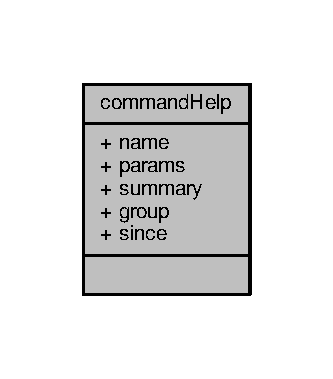
\includegraphics[width=160pt]{structcommandHelp__coll__graph}
\end{center}
\end{figure}
\subsection*{Data Fields}
\begin{DoxyCompactItemize}
\item 
\mbox{\Hypertarget{structcommandHelp_af9eb2e7147a85ca61399a9362d8f3bca}\label{structcommandHelp_af9eb2e7147a85ca61399a9362d8f3bca}} 
char $\ast$ {\bfseries name}
\item 
\mbox{\Hypertarget{structcommandHelp_a2f79db81119f42010852d00341e3d23e}\label{structcommandHelp_a2f79db81119f42010852d00341e3d23e}} 
char $\ast$ {\bfseries params}
\item 
\mbox{\Hypertarget{structcommandHelp_ad4ea8c85da889c0e3afb61a753ace373}\label{structcommandHelp_ad4ea8c85da889c0e3afb61a753ace373}} 
char $\ast$ {\bfseries summary}
\item 
\mbox{\Hypertarget{structcommandHelp_aa62d526b0ceb5e0840f1ebc710e2e31d}\label{structcommandHelp_aa62d526b0ceb5e0840f1ebc710e2e31d}} 
int {\bfseries group}
\item 
\mbox{\Hypertarget{structcommandHelp_a8d06ba546d92db2e1a4590eaa1116c1f}\label{structcommandHelp_a8d06ba546d92db2e1a4590eaa1116c1f}} 
char $\ast$ {\bfseries since}
\end{DoxyCompactItemize}


\subsection{Detailed Description}


Definition at line \hyperlink{help_8h_source_l00023}{23} of file \hyperlink{help_8h_source}{help.\+h}.



\subsection{Field Documentation}
\mbox{\Hypertarget{structcommandHelp_aa62d526b0ceb5e0840f1ebc710e2e31d}\label{structcommandHelp_aa62d526b0ceb5e0840f1ebc710e2e31d}} 
\index{command\+Help@{command\+Help}!group@{group}}
\index{group@{group}!command\+Help@{command\+Help}}
\subsubsection{\texorpdfstring{group}{group}}
{\footnotesize\ttfamily int command\+Help\+::group}



Definition at line \hyperlink{help_8h_source_l00027}{27} of file \hyperlink{help_8h_source}{help.\+h}.

\mbox{\Hypertarget{structcommandHelp_af9eb2e7147a85ca61399a9362d8f3bca}\label{structcommandHelp_af9eb2e7147a85ca61399a9362d8f3bca}} 
\index{command\+Help@{command\+Help}!name@{name}}
\index{name@{name}!command\+Help@{command\+Help}}
\subsubsection{\texorpdfstring{name}{name}}
{\footnotesize\ttfamily char$\ast$ command\+Help\+::name}



Definition at line \hyperlink{help_8h_source_l00024}{24} of file \hyperlink{help_8h_source}{help.\+h}.

\mbox{\Hypertarget{structcommandHelp_a2f79db81119f42010852d00341e3d23e}\label{structcommandHelp_a2f79db81119f42010852d00341e3d23e}} 
\index{command\+Help@{command\+Help}!params@{params}}
\index{params@{params}!command\+Help@{command\+Help}}
\subsubsection{\texorpdfstring{params}{params}}
{\footnotesize\ttfamily char$\ast$ command\+Help\+::params}



Definition at line \hyperlink{help_8h_source_l00025}{25} of file \hyperlink{help_8h_source}{help.\+h}.

\mbox{\Hypertarget{structcommandHelp_a8d06ba546d92db2e1a4590eaa1116c1f}\label{structcommandHelp_a8d06ba546d92db2e1a4590eaa1116c1f}} 
\index{command\+Help@{command\+Help}!since@{since}}
\index{since@{since}!command\+Help@{command\+Help}}
\subsubsection{\texorpdfstring{since}{since}}
{\footnotesize\ttfamily char$\ast$ command\+Help\+::since}



Definition at line \hyperlink{help_8h_source_l00028}{28} of file \hyperlink{help_8h_source}{help.\+h}.

\mbox{\Hypertarget{structcommandHelp_ad4ea8c85da889c0e3afb61a753ace373}\label{structcommandHelp_ad4ea8c85da889c0e3afb61a753ace373}} 
\index{command\+Help@{command\+Help}!summary@{summary}}
\index{summary@{summary}!command\+Help@{command\+Help}}
\subsubsection{\texorpdfstring{summary}{summary}}
{\footnotesize\ttfamily char$\ast$ command\+Help\+::summary}



Definition at line \hyperlink{help_8h_source_l00026}{26} of file \hyperlink{help_8h_source}{help.\+h}.



The documentation for this struct was generated from the following file\+:\begin{DoxyCompactItemize}
\item 
src/help.\+h\end{DoxyCompactItemize}

\hypertarget{structconfigEnum}{}\section{config\+Enum Struct Reference}
\label{structconfigEnum}\index{config\+Enum@{config\+Enum}}


Collaboration diagram for config\+Enum\+:\nopagebreak
\begin{figure}[H]
\begin{center}
\leavevmode
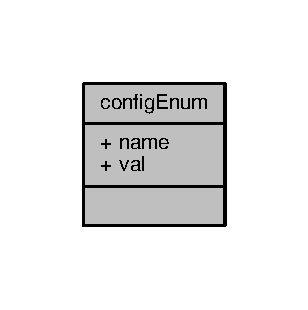
\includegraphics[width=148pt]{structconfigEnum__coll__graph}
\end{center}
\end{figure}
\subsection*{Data Fields}
\begin{DoxyCompactItemize}
\item 
\mbox{\Hypertarget{structconfigEnum_a6160a6cda270a7da6d69238e1543220c}\label{structconfigEnum_a6160a6cda270a7da6d69238e1543220c}} 
const char $\ast$ {\bfseries name}
\item 
\mbox{\Hypertarget{structconfigEnum_ac241b68cfa212a23daac1b48de339aa6}\label{structconfigEnum_ac241b68cfa212a23daac1b48de339aa6}} 
const int {\bfseries val}
\end{DoxyCompactItemize}


\subsection{Detailed Description}


Definition at line \hyperlink{config_8c_source_l00041}{41} of file \hyperlink{config_8c_source}{config.\+c}.



\subsection{Field Documentation}
\mbox{\Hypertarget{structconfigEnum_a6160a6cda270a7da6d69238e1543220c}\label{structconfigEnum_a6160a6cda270a7da6d69238e1543220c}} 
\index{config\+Enum@{config\+Enum}!name@{name}}
\index{name@{name}!config\+Enum@{config\+Enum}}
\subsubsection{\texorpdfstring{name}{name}}
{\footnotesize\ttfamily const char$\ast$ config\+Enum\+::name}



Definition at line \hyperlink{config_8c_source_l00042}{42} of file \hyperlink{config_8c_source}{config.\+c}.

\mbox{\Hypertarget{structconfigEnum_ac241b68cfa212a23daac1b48de339aa6}\label{structconfigEnum_ac241b68cfa212a23daac1b48de339aa6}} 
\index{config\+Enum@{config\+Enum}!val@{val}}
\index{val@{val}!config\+Enum@{config\+Enum}}
\subsubsection{\texorpdfstring{val}{val}}
{\footnotesize\ttfamily const int config\+Enum\+::val}



Definition at line \hyperlink{config_8c_source_l00043}{43} of file \hyperlink{config_8c_source}{config.\+c}.



The documentation for this struct was generated from the following file\+:\begin{DoxyCompactItemize}
\item 
src/config.\+c\end{DoxyCompactItemize}

\hypertarget{structdict}{}\section{dict Struct Reference}
\label{structdict}\index{dict@{dict}}


Collaboration diagram for dict\+:\nopagebreak
\begin{figure}[H]
\begin{center}
\leavevmode
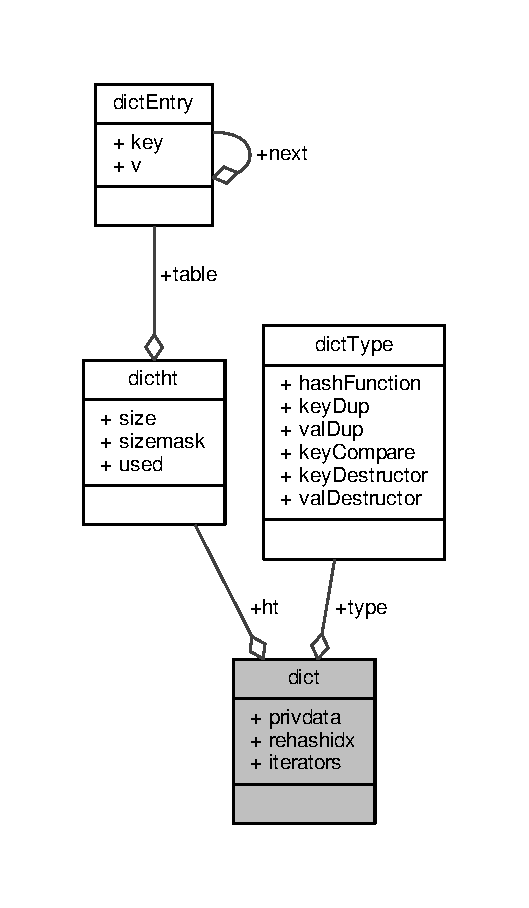
\includegraphics[width=254pt]{structdict__coll__graph}
\end{center}
\end{figure}
\subsection*{Data Fields}
\begin{DoxyCompactItemize}
\item 
\mbox{\Hypertarget{structdict_a89da3d5d54bd930937587a3c411af5fd}\label{structdict_a89da3d5d54bd930937587a3c411af5fd}} 
\hyperlink{structdictType}{dict\+Type} $\ast$ {\bfseries type}
\item 
\mbox{\Hypertarget{structdict_a36ce9f4e7d035fa4d7d2886f30b6a9af}\label{structdict_a36ce9f4e7d035fa4d7d2886f30b6a9af}} 
void $\ast$ {\bfseries privdata}
\item 
\mbox{\Hypertarget{structdict_a5ed6a359a0f2da7f88c4cc352218445a}\label{structdict_a5ed6a359a0f2da7f88c4cc352218445a}} 
\hyperlink{structdictht}{dictht} {\bfseries ht} \mbox{[}2\mbox{]}
\item 
\mbox{\Hypertarget{structdict_aa6aeb098acd50b590319317ad8811b58}\label{structdict_aa6aeb098acd50b590319317ad8811b58}} 
long {\bfseries rehashidx}
\item 
\mbox{\Hypertarget{structdict_a936aefce2677e310e5ecb5943558d614}\label{structdict_a936aefce2677e310e5ecb5943558d614}} 
unsigned long {\bfseries iterators}
\end{DoxyCompactItemize}


\subsection{Detailed Description}


Definition at line \hyperlink{dict_8h_source_l00076}{76} of file \hyperlink{dict_8h_source}{dict.\+h}.



\subsection{Field Documentation}
\mbox{\Hypertarget{structdict_a5ed6a359a0f2da7f88c4cc352218445a}\label{structdict_a5ed6a359a0f2da7f88c4cc352218445a}} 
\index{dict@{dict}!ht@{ht}}
\index{ht@{ht}!dict@{dict}}
\subsubsection{\texorpdfstring{ht}{ht}}
{\footnotesize\ttfamily \hyperlink{structdictht}{dictht} dict\+::ht\mbox{[}2\mbox{]}}



Definition at line \hyperlink{dict_8h_source_l00079}{79} of file \hyperlink{dict_8h_source}{dict.\+h}.

\mbox{\Hypertarget{structdict_a936aefce2677e310e5ecb5943558d614}\label{structdict_a936aefce2677e310e5ecb5943558d614}} 
\index{dict@{dict}!iterators@{iterators}}
\index{iterators@{iterators}!dict@{dict}}
\subsubsection{\texorpdfstring{iterators}{iterators}}
{\footnotesize\ttfamily unsigned long dict\+::iterators}



Definition at line \hyperlink{dict_8h_source_l00081}{81} of file \hyperlink{dict_8h_source}{dict.\+h}.

\mbox{\Hypertarget{structdict_a36ce9f4e7d035fa4d7d2886f30b6a9af}\label{structdict_a36ce9f4e7d035fa4d7d2886f30b6a9af}} 
\index{dict@{dict}!privdata@{privdata}}
\index{privdata@{privdata}!dict@{dict}}
\subsubsection{\texorpdfstring{privdata}{privdata}}
{\footnotesize\ttfamily void$\ast$ dict\+::privdata}



Definition at line \hyperlink{dict_8h_source_l00078}{78} of file \hyperlink{dict_8h_source}{dict.\+h}.

\mbox{\Hypertarget{structdict_aa6aeb098acd50b590319317ad8811b58}\label{structdict_aa6aeb098acd50b590319317ad8811b58}} 
\index{dict@{dict}!rehashidx@{rehashidx}}
\index{rehashidx@{rehashidx}!dict@{dict}}
\subsubsection{\texorpdfstring{rehashidx}{rehashidx}}
{\footnotesize\ttfamily long dict\+::rehashidx}



Definition at line \hyperlink{dict_8h_source_l00080}{80} of file \hyperlink{dict_8h_source}{dict.\+h}.

\mbox{\Hypertarget{structdict_a89da3d5d54bd930937587a3c411af5fd}\label{structdict_a89da3d5d54bd930937587a3c411af5fd}} 
\index{dict@{dict}!type@{type}}
\index{type@{type}!dict@{dict}}
\subsubsection{\texorpdfstring{type}{type}}
{\footnotesize\ttfamily \hyperlink{structdictType}{dict\+Type}$\ast$ dict\+::type}



Definition at line \hyperlink{dict_8h_source_l00077}{77} of file \hyperlink{dict_8h_source}{dict.\+h}.



The documentation for this struct was generated from the following file\+:\begin{DoxyCompactItemize}
\item 
src/dict.\+h\end{DoxyCompactItemize}

\hypertarget{structdictEntry}{}\section{dict\+Entry Struct Reference}
\label{structdictEntry}\index{dict\+Entry@{dict\+Entry}}


Collaboration diagram for dict\+Entry\+:\nopagebreak
\begin{figure}[H]
\begin{center}
\leavevmode
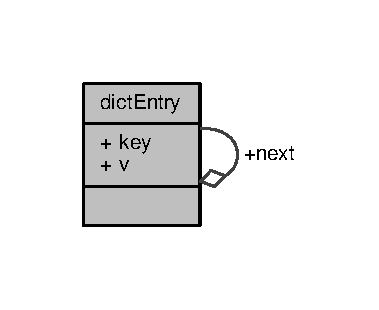
\includegraphics[width=182pt]{structdictEntry__coll__graph}
\end{center}
\end{figure}
\subsection*{Data Fields}
\begin{DoxyCompactItemize}
\item 
\mbox{\Hypertarget{structdictEntry_a1cc436243330e4ac0a1d7d07e5a16ce0}\label{structdictEntry_a1cc436243330e4ac0a1d7d07e5a16ce0}} 
void $\ast$ {\bfseries key}
\item 
\mbox{\Hypertarget{structdictEntry_aab34aa7e370a74652ef12d42b96a44d9}\label{structdictEntry_aab34aa7e370a74652ef12d42b96a44d9}} 
\begin{tabbing}
xx\=xx\=xx\=xx\=xx\=xx\=xx\=xx\=xx\=\kill
union \{\\
\mbox{\Hypertarget{structdictEntry_ae0908b1cf89b6a18ada5063eb2ab1374}\label{structdictEntry_ae0908b1cf89b6a18ada5063eb2ab1374}} 
void $\ast$ {\bfseries val}\\
\mbox{\Hypertarget{structdictEntry_aa6c27a4767bc8919f656080b1bf25ed6}\label{structdictEntry_aa6c27a4767bc8919f656080b1bf25ed6}} 
uint64\_t {\bfseries u64}\\
\mbox{\Hypertarget{structdictEntry_a846a60e6c9a0910f0481e5e38f103ebe}\label{structdictEntry_a846a60e6c9a0910f0481e5e38f103ebe}} 
int64\_t {\bfseries s64}\\
\mbox{\Hypertarget{structdictEntry_ad52f3c5c9135b2a55cad243a5599c1d8}\label{structdictEntry_ad52f3c5c9135b2a55cad243a5599c1d8}} 
double {\bfseries d}\\
\} {\bfseries v}\\

\end{tabbing}\item 
\mbox{\Hypertarget{structdictEntry_ae3d8892babea304bd7e2aded824586dd}\label{structdictEntry_ae3d8892babea304bd7e2aded824586dd}} 
struct \hyperlink{structdictEntry}{dict\+Entry} $\ast$ {\bfseries next}
\end{DoxyCompactItemize}


\subsection{Detailed Description}


Definition at line \hyperlink{dict_8h_source_l00047}{47} of file \hyperlink{dict_8h_source}{dict.\+h}.



\subsection{Field Documentation}
\mbox{\Hypertarget{structdictEntry_a1cc436243330e4ac0a1d7d07e5a16ce0}\label{structdictEntry_a1cc436243330e4ac0a1d7d07e5a16ce0}} 
\index{dict\+Entry@{dict\+Entry}!key@{key}}
\index{key@{key}!dict\+Entry@{dict\+Entry}}
\subsubsection{\texorpdfstring{key}{key}}
{\footnotesize\ttfamily void$\ast$ dict\+Entry\+::key}



Definition at line \hyperlink{dict_8h_source_l00048}{48} of file \hyperlink{dict_8h_source}{dict.\+h}.

\mbox{\Hypertarget{structdictEntry_ae3d8892babea304bd7e2aded824586dd}\label{structdictEntry_ae3d8892babea304bd7e2aded824586dd}} 
\index{dict\+Entry@{dict\+Entry}!next@{next}}
\index{next@{next}!dict\+Entry@{dict\+Entry}}
\subsubsection{\texorpdfstring{next}{next}}
{\footnotesize\ttfamily struct \hyperlink{structdictEntry}{dict\+Entry}$\ast$ dict\+Entry\+::next}



Definition at line \hyperlink{dict_8h_source_l00055}{55} of file \hyperlink{dict_8h_source}{dict.\+h}.

\mbox{\Hypertarget{structdictEntry_aab34aa7e370a74652ef12d42b96a44d9}\label{structdictEntry_aab34aa7e370a74652ef12d42b96a44d9}} 
\index{dict\+Entry@{dict\+Entry}!v@{v}}
\index{v@{v}!dict\+Entry@{dict\+Entry}}
\subsubsection{\texorpdfstring{v}{v}}
{\footnotesize\ttfamily union \{ ... \}   dict\+Entry\+::v}



The documentation for this struct was generated from the following file\+:\begin{DoxyCompactItemize}
\item 
src/dict.\+h\end{DoxyCompactItemize}

\hypertarget{uniondictEntry_8v}{}\section{dict\+Entry.\+v Union Reference}
\label{uniondictEntry_8v}\index{dict\+Entry.\+v@{dict\+Entry.\+v}}


Collaboration diagram for dict\+Entry.\+v\+:\nopagebreak
\begin{figure}[H]
\begin{center}
\leavevmode
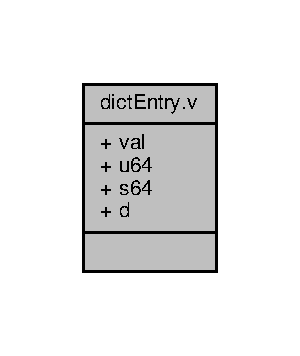
\includegraphics[width=144pt]{uniondictEntry_8v__coll__graph}
\end{center}
\end{figure}
\subsection*{Data Fields}
\begin{DoxyCompactItemize}
\item 
\mbox{\Hypertarget{uniondictEntry_8v_a3a6d0284e743dc4a9b86f97d6dd1a3bf}\label{uniondictEntry_8v_a3a6d0284e743dc4a9b86f97d6dd1a3bf}} 
void $\ast$ {\bfseries val}
\item 
\mbox{\Hypertarget{uniondictEntry_8v_a476bf781fb66b23778b1004edc3a1028}\label{uniondictEntry_8v_a476bf781fb66b23778b1004edc3a1028}} 
uint64\+\_\+t {\bfseries u64}
\item 
\mbox{\Hypertarget{uniondictEntry_8v_a1919b6c3d1a9b2545d55cd7176afd38b}\label{uniondictEntry_8v_a1919b6c3d1a9b2545d55cd7176afd38b}} 
int64\+\_\+t {\bfseries s64}
\item 
\mbox{\Hypertarget{uniondictEntry_8v_a8277e0910d750195b448797616e091ad}\label{uniondictEntry_8v_a8277e0910d750195b448797616e091ad}} 
double {\bfseries d}
\end{DoxyCompactItemize}


\subsection{Detailed Description}


Definition at line \hyperlink{dict_8h_source_l00049}{49} of file \hyperlink{dict_8h_source}{dict.\+h}.



\subsection{Field Documentation}
\mbox{\Hypertarget{uniondictEntry_8v_a8277e0910d750195b448797616e091ad}\label{uniondictEntry_8v_a8277e0910d750195b448797616e091ad}} 
\index{dict\+Entry.\+v@{dict\+Entry.\+v}!d@{d}}
\index{d@{d}!dict\+Entry.\+v@{dict\+Entry.\+v}}
\subsubsection{\texorpdfstring{d}{d}}
{\footnotesize\ttfamily }

\mbox{\Hypertarget{uniondictEntry_8v_a1919b6c3d1a9b2545d55cd7176afd38b}\label{uniondictEntry_8v_a1919b6c3d1a9b2545d55cd7176afd38b}} 
\index{dict\+Entry.\+v@{dict\+Entry.\+v}!s64@{s64}}
\index{s64@{s64}!dict\+Entry.\+v@{dict\+Entry.\+v}}
\subsubsection{\texorpdfstring{s64}{s64}}
{\footnotesize\ttfamily }

\mbox{\Hypertarget{uniondictEntry_8v_a476bf781fb66b23778b1004edc3a1028}\label{uniondictEntry_8v_a476bf781fb66b23778b1004edc3a1028}} 
\index{dict\+Entry.\+v@{dict\+Entry.\+v}!u64@{u64}}
\index{u64@{u64}!dict\+Entry.\+v@{dict\+Entry.\+v}}
\subsubsection{\texorpdfstring{u64}{u64}}
{\footnotesize\ttfamily }

\mbox{\Hypertarget{uniondictEntry_8v_a3a6d0284e743dc4a9b86f97d6dd1a3bf}\label{uniondictEntry_8v_a3a6d0284e743dc4a9b86f97d6dd1a3bf}} 
\index{dict\+Entry.\+v@{dict\+Entry.\+v}!val@{val}}
\index{val@{val}!dict\+Entry.\+v@{dict\+Entry.\+v}}
\subsubsection{\texorpdfstring{val}{val}}
{\footnotesize\ttfamily }



The documentation for this union was generated from the following files\+:
\hypertarget{structdictht}{}\section{dictht Struct Reference}
\label{structdictht}\index{dictht@{dictht}}


Collaboration diagram for dictht\+:\nopagebreak
\begin{figure}[H]
\begin{center}
\leavevmode
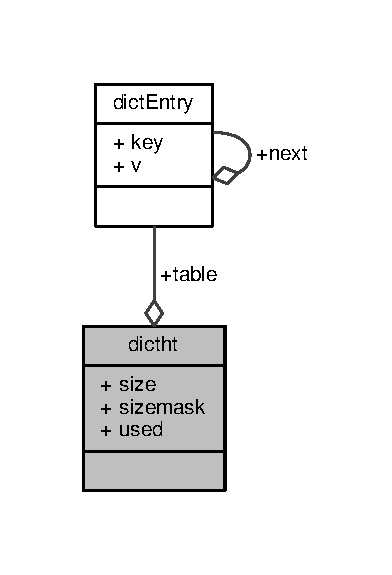
\includegraphics[width=188pt]{structdictht__coll__graph}
\end{center}
\end{figure}
\subsection*{Data Fields}
\begin{DoxyCompactItemize}
\item 
\mbox{\Hypertarget{structdictht_af723bb6ba2e520eab1c53500e2e5c835}\label{structdictht_af723bb6ba2e520eab1c53500e2e5c835}} 
\hyperlink{structdictEntry}{dict\+Entry} $\ast$$\ast$ {\bfseries table}
\item 
\mbox{\Hypertarget{structdictht_ac8ef79c0bdbbddfc028e1c16794cd261}\label{structdictht_ac8ef79c0bdbbddfc028e1c16794cd261}} 
unsigned long {\bfseries size}
\item 
\mbox{\Hypertarget{structdictht_a72530b5a4f8cba9e264242004c273653}\label{structdictht_a72530b5a4f8cba9e264242004c273653}} 
unsigned long {\bfseries sizemask}
\item 
\mbox{\Hypertarget{structdictht_ab67ac2d13aa52a10fb0085f93cf3d4dd}\label{structdictht_ab67ac2d13aa52a10fb0085f93cf3d4dd}} 
unsigned long {\bfseries used}
\end{DoxyCompactItemize}


\subsection{Detailed Description}


Definition at line \hyperlink{dict_8h_source_l00069}{69} of file \hyperlink{dict_8h_source}{dict.\+h}.



\subsection{Field Documentation}
\mbox{\Hypertarget{structdictht_ac8ef79c0bdbbddfc028e1c16794cd261}\label{structdictht_ac8ef79c0bdbbddfc028e1c16794cd261}} 
\index{dictht@{dictht}!size@{size}}
\index{size@{size}!dictht@{dictht}}
\subsubsection{\texorpdfstring{size}{size}}
{\footnotesize\ttfamily unsigned long dictht\+::size}



Definition at line \hyperlink{dict_8h_source_l00071}{71} of file \hyperlink{dict_8h_source}{dict.\+h}.

\mbox{\Hypertarget{structdictht_a72530b5a4f8cba9e264242004c273653}\label{structdictht_a72530b5a4f8cba9e264242004c273653}} 
\index{dictht@{dictht}!sizemask@{sizemask}}
\index{sizemask@{sizemask}!dictht@{dictht}}
\subsubsection{\texorpdfstring{sizemask}{sizemask}}
{\footnotesize\ttfamily unsigned long dictht\+::sizemask}



Definition at line \hyperlink{dict_8h_source_l00072}{72} of file \hyperlink{dict_8h_source}{dict.\+h}.

\mbox{\Hypertarget{structdictht_af723bb6ba2e520eab1c53500e2e5c835}\label{structdictht_af723bb6ba2e520eab1c53500e2e5c835}} 
\index{dictht@{dictht}!table@{table}}
\index{table@{table}!dictht@{dictht}}
\subsubsection{\texorpdfstring{table}{table}}
{\footnotesize\ttfamily \hyperlink{structdictEntry}{dict\+Entry}$\ast$$\ast$ dictht\+::table}



Definition at line \hyperlink{dict_8h_source_l00070}{70} of file \hyperlink{dict_8h_source}{dict.\+h}.

\mbox{\Hypertarget{structdictht_ab67ac2d13aa52a10fb0085f93cf3d4dd}\label{structdictht_ab67ac2d13aa52a10fb0085f93cf3d4dd}} 
\index{dictht@{dictht}!used@{used}}
\index{used@{used}!dictht@{dictht}}
\subsubsection{\texorpdfstring{used}{used}}
{\footnotesize\ttfamily unsigned long dictht\+::used}



Definition at line \hyperlink{dict_8h_source_l00073}{73} of file \hyperlink{dict_8h_source}{dict.\+h}.



The documentation for this struct was generated from the following file\+:\begin{DoxyCompactItemize}
\item 
src/dict.\+h\end{DoxyCompactItemize}

\hypertarget{structdictIterator}{}\section{dict\+Iterator Struct Reference}
\label{structdictIterator}\index{dict\+Iterator@{dict\+Iterator}}


Collaboration diagram for dict\+Iterator\+:\nopagebreak
\begin{figure}[H]
\begin{center}
\leavevmode
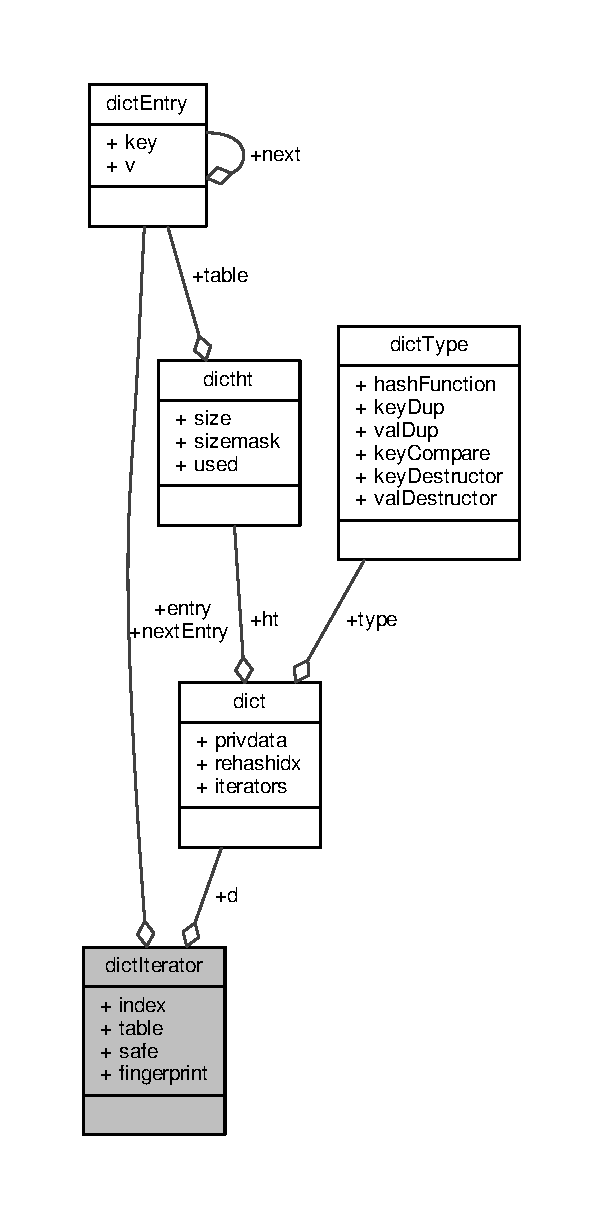
\includegraphics[height=550pt]{structdictIterator__coll__graph}
\end{center}
\end{figure}
\subsection*{Data Fields}
\begin{DoxyCompactItemize}
\item 
\mbox{\Hypertarget{structdictIterator_a1d2b99eef5ff04edcd4ac1d2e44cee03}\label{structdictIterator_a1d2b99eef5ff04edcd4ac1d2e44cee03}} 
\hyperlink{structdict}{dict} $\ast$ {\bfseries d}
\item 
\mbox{\Hypertarget{structdictIterator_a3e0798e8d5e0906fbd6181a2588b3e98}\label{structdictIterator_a3e0798e8d5e0906fbd6181a2588b3e98}} 
long {\bfseries index}
\item 
\mbox{\Hypertarget{structdictIterator_aea5d0c657d1dbea4bde6e7915c305598}\label{structdictIterator_aea5d0c657d1dbea4bde6e7915c305598}} 
int {\bfseries table}
\item 
\mbox{\Hypertarget{structdictIterator_af8dd20e8e8bdab1e0331015005aba390}\label{structdictIterator_af8dd20e8e8bdab1e0331015005aba390}} 
int {\bfseries safe}
\item 
\mbox{\Hypertarget{structdictIterator_a5bbcc9b0c792e1ee68c6a4ed049da816}\label{structdictIterator_a5bbcc9b0c792e1ee68c6a4ed049da816}} 
\hyperlink{structdictEntry}{dict\+Entry} $\ast$ {\bfseries entry}
\item 
\mbox{\Hypertarget{structdictIterator_aa030de14f2996420066a50980581d0d8}\label{structdictIterator_aa030de14f2996420066a50980581d0d8}} 
\hyperlink{structdictEntry}{dict\+Entry} $\ast$ {\bfseries next\+Entry}
\item 
\mbox{\Hypertarget{structdictIterator_a88066bf1d96483011eaf2cf73ee4f0a0}\label{structdictIterator_a88066bf1d96483011eaf2cf73ee4f0a0}} 
long long {\bfseries fingerprint}
\end{DoxyCompactItemize}


\subsection{Detailed Description}


Definition at line \hyperlink{dict_8h_source_l00088}{88} of file \hyperlink{dict_8h_source}{dict.\+h}.



\subsection{Field Documentation}
\mbox{\Hypertarget{structdictIterator_a1d2b99eef5ff04edcd4ac1d2e44cee03}\label{structdictIterator_a1d2b99eef5ff04edcd4ac1d2e44cee03}} 
\index{dict\+Iterator@{dict\+Iterator}!d@{d}}
\index{d@{d}!dict\+Iterator@{dict\+Iterator}}
\subsubsection{\texorpdfstring{d}{d}}
{\footnotesize\ttfamily \hyperlink{structdict}{dict}$\ast$ dict\+Iterator\+::d}



Definition at line \hyperlink{dict_8h_source_l00089}{89} of file \hyperlink{dict_8h_source}{dict.\+h}.

\mbox{\Hypertarget{structdictIterator_a5bbcc9b0c792e1ee68c6a4ed049da816}\label{structdictIterator_a5bbcc9b0c792e1ee68c6a4ed049da816}} 
\index{dict\+Iterator@{dict\+Iterator}!entry@{entry}}
\index{entry@{entry}!dict\+Iterator@{dict\+Iterator}}
\subsubsection{\texorpdfstring{entry}{entry}}
{\footnotesize\ttfamily \hyperlink{structdictEntry}{dict\+Entry}$\ast$ dict\+Iterator\+::entry}



Definition at line \hyperlink{dict_8h_source_l00092}{92} of file \hyperlink{dict_8h_source}{dict.\+h}.

\mbox{\Hypertarget{structdictIterator_a88066bf1d96483011eaf2cf73ee4f0a0}\label{structdictIterator_a88066bf1d96483011eaf2cf73ee4f0a0}} 
\index{dict\+Iterator@{dict\+Iterator}!fingerprint@{fingerprint}}
\index{fingerprint@{fingerprint}!dict\+Iterator@{dict\+Iterator}}
\subsubsection{\texorpdfstring{fingerprint}{fingerprint}}
{\footnotesize\ttfamily long long dict\+Iterator\+::fingerprint}



Definition at line \hyperlink{dict_8h_source_l00094}{94} of file \hyperlink{dict_8h_source}{dict.\+h}.

\mbox{\Hypertarget{structdictIterator_a3e0798e8d5e0906fbd6181a2588b3e98}\label{structdictIterator_a3e0798e8d5e0906fbd6181a2588b3e98}} 
\index{dict\+Iterator@{dict\+Iterator}!index@{index}}
\index{index@{index}!dict\+Iterator@{dict\+Iterator}}
\subsubsection{\texorpdfstring{index}{index}}
{\footnotesize\ttfamily long dict\+Iterator\+::index}



Definition at line \hyperlink{dict_8h_source_l00090}{90} of file \hyperlink{dict_8h_source}{dict.\+h}.

\mbox{\Hypertarget{structdictIterator_aa030de14f2996420066a50980581d0d8}\label{structdictIterator_aa030de14f2996420066a50980581d0d8}} 
\index{dict\+Iterator@{dict\+Iterator}!next\+Entry@{next\+Entry}}
\index{next\+Entry@{next\+Entry}!dict\+Iterator@{dict\+Iterator}}
\subsubsection{\texorpdfstring{next\+Entry}{nextEntry}}
{\footnotesize\ttfamily \hyperlink{structdictEntry}{dict\+Entry} $\ast$ dict\+Iterator\+::next\+Entry}



Definition at line \hyperlink{dict_8h_source_l00092}{92} of file \hyperlink{dict_8h_source}{dict.\+h}.

\mbox{\Hypertarget{structdictIterator_af8dd20e8e8bdab1e0331015005aba390}\label{structdictIterator_af8dd20e8e8bdab1e0331015005aba390}} 
\index{dict\+Iterator@{dict\+Iterator}!safe@{safe}}
\index{safe@{safe}!dict\+Iterator@{dict\+Iterator}}
\subsubsection{\texorpdfstring{safe}{safe}}
{\footnotesize\ttfamily int dict\+Iterator\+::safe}



Definition at line \hyperlink{dict_8h_source_l00091}{91} of file \hyperlink{dict_8h_source}{dict.\+h}.

\mbox{\Hypertarget{structdictIterator_aea5d0c657d1dbea4bde6e7915c305598}\label{structdictIterator_aea5d0c657d1dbea4bde6e7915c305598}} 
\index{dict\+Iterator@{dict\+Iterator}!table@{table}}
\index{table@{table}!dict\+Iterator@{dict\+Iterator}}
\subsubsection{\texorpdfstring{table}{table}}
{\footnotesize\ttfamily int dict\+Iterator\+::table}



Definition at line \hyperlink{dict_8h_source_l00091}{91} of file \hyperlink{dict_8h_source}{dict.\+h}.



The documentation for this struct was generated from the following file\+:\begin{DoxyCompactItemize}
\item 
src/dict.\+h\end{DoxyCompactItemize}

\hypertarget{structdictType}{}\section{dict\+Type Struct Reference}
\label{structdictType}\index{dict\+Type@{dict\+Type}}


Collaboration diagram for dict\+Type\+:\nopagebreak
\begin{figure}[H]
\begin{center}
\leavevmode
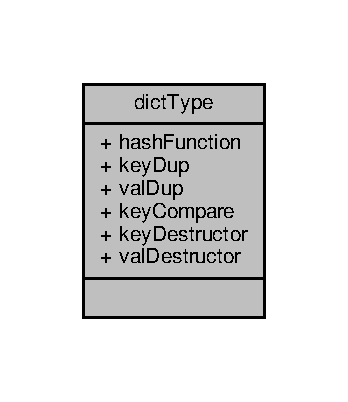
\includegraphics[width=167pt]{structdictType__coll__graph}
\end{center}
\end{figure}
\subsection*{Data Fields}
\begin{DoxyCompactItemize}
\item 
\mbox{\Hypertarget{structdictType_a5163c6331e157f62a678cf30d7c7e334}\label{structdictType_a5163c6331e157f62a678cf30d7c7e334}} 
uint64\+\_\+t($\ast$ {\bfseries hash\+Function} )(const void $\ast$key)
\item 
\mbox{\Hypertarget{structdictType_a9addb7c29c6082073a17743b44b0d563}\label{structdictType_a9addb7c29c6082073a17743b44b0d563}} 
void $\ast$($\ast$ {\bfseries key\+Dup} )(void $\ast$privdata, const void $\ast$key)
\item 
\mbox{\Hypertarget{structdictType_ad9752f0251c3121b2fc96be02383eee2}\label{structdictType_ad9752f0251c3121b2fc96be02383eee2}} 
void $\ast$($\ast$ {\bfseries val\+Dup} )(void $\ast$privdata, const void $\ast$obj)
\item 
\mbox{\Hypertarget{structdictType_abc4e87fe80173aa50732c049d3be96b5}\label{structdictType_abc4e87fe80173aa50732c049d3be96b5}} 
int($\ast$ {\bfseries key\+Compare} )(void $\ast$privdata, const void $\ast$key1, const void $\ast$key2)
\item 
\mbox{\Hypertarget{structdictType_a448ee05f531f872a05a2cdafccb5ecc4}\label{structdictType_a448ee05f531f872a05a2cdafccb5ecc4}} 
void($\ast$ {\bfseries key\+Destructor} )(void $\ast$privdata, void $\ast$key)
\item 
\mbox{\Hypertarget{structdictType_a491b1283bac257f1573e38479131b18f}\label{structdictType_a491b1283bac257f1573e38479131b18f}} 
void($\ast$ {\bfseries val\+Destructor} )(void $\ast$privdata, void $\ast$obj)
\end{DoxyCompactItemize}


\subsection{Detailed Description}


Definition at line \hyperlink{dict_8h_source_l00058}{58} of file \hyperlink{dict_8h_source}{dict.\+h}.



The documentation for this struct was generated from the following file\+:\begin{DoxyCompactItemize}
\item 
src/dict.\+h\end{DoxyCompactItemize}

\hypertarget{structdistsamples}{}\section{distsamples Struct Reference}
\label{structdistsamples}\index{distsamples@{distsamples}}


Collaboration diagram for distsamples\+:\nopagebreak
\begin{figure}[H]
\begin{center}
\leavevmode
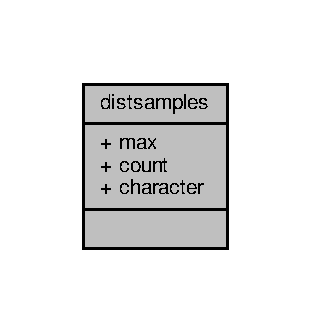
\includegraphics[width=149pt]{structdistsamples__coll__graph}
\end{center}
\end{figure}
\subsection*{Data Fields}
\begin{DoxyCompactItemize}
\item 
\mbox{\Hypertarget{structdistsamples_a42cb229a35440667716cbe5dd5da4f0e}\label{structdistsamples_a42cb229a35440667716cbe5dd5da4f0e}} 
long long {\bfseries max}
\item 
\mbox{\Hypertarget{structdistsamples_a7c254d479072c13b847895fbc2e16c23}\label{structdistsamples_a7c254d479072c13b847895fbc2e16c23}} 
long long {\bfseries count}
\item 
\mbox{\Hypertarget{structdistsamples_a8cc486cc09fcdb634ea9480b57958ca0}\label{structdistsamples_a8cc486cc09fcdb634ea9480b57958ca0}} 
int {\bfseries character}
\end{DoxyCompactItemize}


\subsection{Detailed Description}


Definition at line \hyperlink{redis-cli_8c_source_l01657}{1657} of file \hyperlink{redis-cli_8c_source}{redis-\/cli.\+c}.



\subsection{Field Documentation}
\mbox{\Hypertarget{structdistsamples_a8cc486cc09fcdb634ea9480b57958ca0}\label{structdistsamples_a8cc486cc09fcdb634ea9480b57958ca0}} 
\index{distsamples@{distsamples}!character@{character}}
\index{character@{character}!distsamples@{distsamples}}
\subsubsection{\texorpdfstring{character}{character}}
{\footnotesize\ttfamily int distsamples\+::character}



Definition at line \hyperlink{redis-cli_8c_source_l01660}{1660} of file \hyperlink{redis-cli_8c_source}{redis-\/cli.\+c}.

\mbox{\Hypertarget{structdistsamples_a7c254d479072c13b847895fbc2e16c23}\label{structdistsamples_a7c254d479072c13b847895fbc2e16c23}} 
\index{distsamples@{distsamples}!count@{count}}
\index{count@{count}!distsamples@{distsamples}}
\subsubsection{\texorpdfstring{count}{count}}
{\footnotesize\ttfamily long long distsamples\+::count}



Definition at line \hyperlink{redis-cli_8c_source_l01659}{1659} of file \hyperlink{redis-cli_8c_source}{redis-\/cli.\+c}.

\mbox{\Hypertarget{structdistsamples_a42cb229a35440667716cbe5dd5da4f0e}\label{structdistsamples_a42cb229a35440667716cbe5dd5da4f0e}} 
\index{distsamples@{distsamples}!max@{max}}
\index{max@{max}!distsamples@{distsamples}}
\subsubsection{\texorpdfstring{max}{max}}
{\footnotesize\ttfamily long long distsamples\+::max}



Definition at line \hyperlink{redis-cli_8c_source_l01658}{1658} of file \hyperlink{redis-cli_8c_source}{redis-\/cli.\+c}.



The documentation for this struct was generated from the following file\+:\begin{DoxyCompactItemize}
\item 
src/redis-\/cli.\+c\end{DoxyCompactItemize}

\hypertarget{structevictionPoolEntry}{}\section{eviction\+Pool\+Entry Struct Reference}
\label{structevictionPoolEntry}\index{eviction\+Pool\+Entry@{eviction\+Pool\+Entry}}


Collaboration diagram for eviction\+Pool\+Entry\+:\nopagebreak
\begin{figure}[H]
\begin{center}
\leavevmode
\includegraphics[width=173pt]{structevictionPoolEntry__coll__graph}
\end{center}
\end{figure}
\subsection*{Data Fields}
\begin{DoxyCompactItemize}
\item 
\mbox{\Hypertarget{structevictionPoolEntry_a1684112289f68796969533d55668564f}\label{structevictionPoolEntry_a1684112289f68796969533d55668564f}} 
unsigned long long {\bfseries idle}
\item 
\mbox{\Hypertarget{structevictionPoolEntry_ab2dd4d387743e8435f5a50f66ae9c9f1}\label{structevictionPoolEntry_ab2dd4d387743e8435f5a50f66ae9c9f1}} 
sds {\bfseries key}
\item 
\mbox{\Hypertarget{structevictionPoolEntry_a57611fdc5a655a808616731b051dd62c}\label{structevictionPoolEntry_a57611fdc5a655a808616731b051dd62c}} 
sds {\bfseries cached}
\item 
\mbox{\Hypertarget{structevictionPoolEntry_a4d28f9d176d4047641f2153b0f7af294}\label{structevictionPoolEntry_a4d28f9d176d4047641f2153b0f7af294}} 
int {\bfseries dbid}
\end{DoxyCompactItemize}


\subsection{Detailed Description}


Definition at line \hyperlink{evict_8c_source_l00054}{54} of file \hyperlink{evict_8c_source}{evict.\+c}.



\subsection{Field Documentation}
\mbox{\Hypertarget{structevictionPoolEntry_a57611fdc5a655a808616731b051dd62c}\label{structevictionPoolEntry_a57611fdc5a655a808616731b051dd62c}} 
\index{eviction\+Pool\+Entry@{eviction\+Pool\+Entry}!cached@{cached}}
\index{cached@{cached}!eviction\+Pool\+Entry@{eviction\+Pool\+Entry}}
\subsubsection{\texorpdfstring{cached}{cached}}
{\footnotesize\ttfamily sds eviction\+Pool\+Entry\+::cached}



Definition at line \hyperlink{evict_8c_source_l00057}{57} of file \hyperlink{evict_8c_source}{evict.\+c}.

\mbox{\Hypertarget{structevictionPoolEntry_a4d28f9d176d4047641f2153b0f7af294}\label{structevictionPoolEntry_a4d28f9d176d4047641f2153b0f7af294}} 
\index{eviction\+Pool\+Entry@{eviction\+Pool\+Entry}!dbid@{dbid}}
\index{dbid@{dbid}!eviction\+Pool\+Entry@{eviction\+Pool\+Entry}}
\subsubsection{\texorpdfstring{dbid}{dbid}}
{\footnotesize\ttfamily int eviction\+Pool\+Entry\+::dbid}



Definition at line \hyperlink{evict_8c_source_l00058}{58} of file \hyperlink{evict_8c_source}{evict.\+c}.

\mbox{\Hypertarget{structevictionPoolEntry_a1684112289f68796969533d55668564f}\label{structevictionPoolEntry_a1684112289f68796969533d55668564f}} 
\index{eviction\+Pool\+Entry@{eviction\+Pool\+Entry}!idle@{idle}}
\index{idle@{idle}!eviction\+Pool\+Entry@{eviction\+Pool\+Entry}}
\subsubsection{\texorpdfstring{idle}{idle}}
{\footnotesize\ttfamily unsigned long long eviction\+Pool\+Entry\+::idle}



Definition at line \hyperlink{evict_8c_source_l00055}{55} of file \hyperlink{evict_8c_source}{evict.\+c}.

\mbox{\Hypertarget{structevictionPoolEntry_ab2dd4d387743e8435f5a50f66ae9c9f1}\label{structevictionPoolEntry_ab2dd4d387743e8435f5a50f66ae9c9f1}} 
\index{eviction\+Pool\+Entry@{eviction\+Pool\+Entry}!key@{key}}
\index{key@{key}!eviction\+Pool\+Entry@{eviction\+Pool\+Entry}}
\subsubsection{\texorpdfstring{key}{key}}
{\footnotesize\ttfamily sds eviction\+Pool\+Entry\+::key}



Definition at line \hyperlink{evict_8c_source_l00056}{56} of file \hyperlink{evict_8c_source}{evict.\+c}.



The documentation for this struct was generated from the following file\+:\begin{DoxyCompactItemize}
\item 
src/evict.\+c\end{DoxyCompactItemize}

\hypertarget{structgeoArray}{}\section{geo\+Array Struct Reference}
\label{structgeoArray}\index{geo\+Array@{geo\+Array}}


Collaboration diagram for geo\+Array\+:\nopagebreak
\begin{figure}[H]
\begin{center}
\leavevmode
\includegraphics[width=145pt]{structgeoArray__coll__graph}
\end{center}
\end{figure}
\subsection*{Data Fields}
\begin{DoxyCompactItemize}
\item 
\mbox{\Hypertarget{structgeoArray_a1cc43cbd466bbd97fd31f446b5820b0d}\label{structgeoArray_a1cc43cbd466bbd97fd31f446b5820b0d}} 
struct \hyperlink{structgeoPoint}{geo\+Point} $\ast$ {\bfseries array}
\item 
\mbox{\Hypertarget{structgeoArray_a2e70eb3d48466cd1e914c0e04c737425}\label{structgeoArray_a2e70eb3d48466cd1e914c0e04c737425}} 
size\+\_\+t {\bfseries buckets}
\item 
\mbox{\Hypertarget{structgeoArray_a4fc493a8a1ebc7855a1fee78376ad595}\label{structgeoArray_a4fc493a8a1ebc7855a1fee78376ad595}} 
size\+\_\+t {\bfseries used}
\end{DoxyCompactItemize}


\subsection{Detailed Description}


Definition at line \hyperlink{geo_8h_source_l00016}{16} of file \hyperlink{geo_8h_source}{geo.\+h}.



\subsection{Field Documentation}
\mbox{\Hypertarget{structgeoArray_a1cc43cbd466bbd97fd31f446b5820b0d}\label{structgeoArray_a1cc43cbd466bbd97fd31f446b5820b0d}} 
\index{geo\+Array@{geo\+Array}!array@{array}}
\index{array@{array}!geo\+Array@{geo\+Array}}
\subsubsection{\texorpdfstring{array}{array}}
{\footnotesize\ttfamily struct \hyperlink{structgeoPoint}{geo\+Point}$\ast$ geo\+Array\+::array}



Definition at line \hyperlink{geo_8h_source_l00017}{17} of file \hyperlink{geo_8h_source}{geo.\+h}.

\mbox{\Hypertarget{structgeoArray_a2e70eb3d48466cd1e914c0e04c737425}\label{structgeoArray_a2e70eb3d48466cd1e914c0e04c737425}} 
\index{geo\+Array@{geo\+Array}!buckets@{buckets}}
\index{buckets@{buckets}!geo\+Array@{geo\+Array}}
\subsubsection{\texorpdfstring{buckets}{buckets}}
{\footnotesize\ttfamily size\+\_\+t geo\+Array\+::buckets}



Definition at line \hyperlink{geo_8h_source_l00018}{18} of file \hyperlink{geo_8h_source}{geo.\+h}.

\mbox{\Hypertarget{structgeoArray_a4fc493a8a1ebc7855a1fee78376ad595}\label{structgeoArray_a4fc493a8a1ebc7855a1fee78376ad595}} 
\index{geo\+Array@{geo\+Array}!used@{used}}
\index{used@{used}!geo\+Array@{geo\+Array}}
\subsubsection{\texorpdfstring{used}{used}}
{\footnotesize\ttfamily size\+\_\+t geo\+Array\+::used}



Definition at line \hyperlink{geo_8h_source_l00019}{19} of file \hyperlink{geo_8h_source}{geo.\+h}.



The documentation for this struct was generated from the following file\+:\begin{DoxyCompactItemize}
\item 
src/geo.\+h\end{DoxyCompactItemize}

\hypertarget{structGeoHashArea}{}\section{Geo\+Hash\+Area Struct Reference}
\label{structGeoHashArea}\index{Geo\+Hash\+Area@{Geo\+Hash\+Area}}


Collaboration diagram for Geo\+Hash\+Area\+:\nopagebreak
\begin{figure}[H]
\begin{center}
\leavevmode
\includegraphics[width=260pt]{structGeoHashArea__coll__graph}
\end{center}
\end{figure}
\subsection*{Data Fields}
\begin{DoxyCompactItemize}
\item 
\mbox{\Hypertarget{structGeoHashArea_a34e84c608242e72dac8643104a51e0e1}\label{structGeoHashArea_a34e84c608242e72dac8643104a51e0e1}} 
\hyperlink{structGeoHashBits}{Geo\+Hash\+Bits} {\bfseries hash}
\item 
\mbox{\Hypertarget{structGeoHashArea_a5c5319cf44c7f8181d5883d01055ef62}\label{structGeoHashArea_a5c5319cf44c7f8181d5883d01055ef62}} 
\hyperlink{structGeoHashRange}{Geo\+Hash\+Range} {\bfseries longitude}
\item 
\mbox{\Hypertarget{structGeoHashArea_a7ca5883bf7c8b3404743d3618b3f62c2}\label{structGeoHashArea_a7ca5883bf7c8b3404743d3618b3f62c2}} 
\hyperlink{structGeoHashRange}{Geo\+Hash\+Range} {\bfseries latitude}
\end{DoxyCompactItemize}


\subsection{Detailed Description}


Definition at line \hyperlink{geohash_8h_source_l00076}{76} of file \hyperlink{geohash_8h_source}{geohash.\+h}.



\subsection{Field Documentation}
\mbox{\Hypertarget{structGeoHashArea_a34e84c608242e72dac8643104a51e0e1}\label{structGeoHashArea_a34e84c608242e72dac8643104a51e0e1}} 
\index{Geo\+Hash\+Area@{Geo\+Hash\+Area}!hash@{hash}}
\index{hash@{hash}!Geo\+Hash\+Area@{Geo\+Hash\+Area}}
\subsubsection{\texorpdfstring{hash}{hash}}
{\footnotesize\ttfamily \hyperlink{structGeoHashBits}{Geo\+Hash\+Bits} Geo\+Hash\+Area\+::hash}



Definition at line \hyperlink{geohash_8h_source_l00077}{77} of file \hyperlink{geohash_8h_source}{geohash.\+h}.

\mbox{\Hypertarget{structGeoHashArea_a7ca5883bf7c8b3404743d3618b3f62c2}\label{structGeoHashArea_a7ca5883bf7c8b3404743d3618b3f62c2}} 
\index{Geo\+Hash\+Area@{Geo\+Hash\+Area}!latitude@{latitude}}
\index{latitude@{latitude}!Geo\+Hash\+Area@{Geo\+Hash\+Area}}
\subsubsection{\texorpdfstring{latitude}{latitude}}
{\footnotesize\ttfamily \hyperlink{structGeoHashRange}{Geo\+Hash\+Range} Geo\+Hash\+Area\+::latitude}



Definition at line \hyperlink{geohash_8h_source_l00079}{79} of file \hyperlink{geohash_8h_source}{geohash.\+h}.

\mbox{\Hypertarget{structGeoHashArea_a5c5319cf44c7f8181d5883d01055ef62}\label{structGeoHashArea_a5c5319cf44c7f8181d5883d01055ef62}} 
\index{Geo\+Hash\+Area@{Geo\+Hash\+Area}!longitude@{longitude}}
\index{longitude@{longitude}!Geo\+Hash\+Area@{Geo\+Hash\+Area}}
\subsubsection{\texorpdfstring{longitude}{longitude}}
{\footnotesize\ttfamily \hyperlink{structGeoHashRange}{Geo\+Hash\+Range} Geo\+Hash\+Area\+::longitude}



Definition at line \hyperlink{geohash_8h_source_l00078}{78} of file \hyperlink{geohash_8h_source}{geohash.\+h}.



The documentation for this struct was generated from the following file\+:\begin{DoxyCompactItemize}
\item 
src/geohash.\+h\end{DoxyCompactItemize}

\hypertarget{structGeoHashBits}{}\section{Geo\+Hash\+Bits Struct Reference}
\label{structGeoHashBits}\index{Geo\+Hash\+Bits@{Geo\+Hash\+Bits}}


Collaboration diagram for Geo\+Hash\+Bits\+:\nopagebreak
\begin{figure}[H]
\begin{center}
\leavevmode
\includegraphics[width=155pt]{structGeoHashBits__coll__graph}
\end{center}
\end{figure}
\subsection*{Data Fields}
\begin{DoxyCompactItemize}
\item 
\mbox{\Hypertarget{structGeoHashBits_ab72063af4534bc9fbfa96c069da5211e}\label{structGeoHashBits_ab72063af4534bc9fbfa96c069da5211e}} 
uint64\+\_\+t {\bfseries bits}
\item 
\mbox{\Hypertarget{structGeoHashBits_aa239ef28dd8d97a7f4eb3c754dce1b90}\label{structGeoHashBits_aa239ef28dd8d97a7f4eb3c754dce1b90}} 
uint8\+\_\+t {\bfseries step}
\end{DoxyCompactItemize}


\subsection{Detailed Description}


Definition at line \hyperlink{geohash_8h_source_l00066}{66} of file \hyperlink{geohash_8h_source}{geohash.\+h}.



\subsection{Field Documentation}
\mbox{\Hypertarget{structGeoHashBits_ab72063af4534bc9fbfa96c069da5211e}\label{structGeoHashBits_ab72063af4534bc9fbfa96c069da5211e}} 
\index{Geo\+Hash\+Bits@{Geo\+Hash\+Bits}!bits@{bits}}
\index{bits@{bits}!Geo\+Hash\+Bits@{Geo\+Hash\+Bits}}
\subsubsection{\texorpdfstring{bits}{bits}}
{\footnotesize\ttfamily uint64\+\_\+t Geo\+Hash\+Bits\+::bits}



Definition at line \hyperlink{geohash_8h_source_l00067}{67} of file \hyperlink{geohash_8h_source}{geohash.\+h}.

\mbox{\Hypertarget{structGeoHashBits_aa239ef28dd8d97a7f4eb3c754dce1b90}\label{structGeoHashBits_aa239ef28dd8d97a7f4eb3c754dce1b90}} 
\index{Geo\+Hash\+Bits@{Geo\+Hash\+Bits}!step@{step}}
\index{step@{step}!Geo\+Hash\+Bits@{Geo\+Hash\+Bits}}
\subsubsection{\texorpdfstring{step}{step}}
{\footnotesize\ttfamily uint8\+\_\+t Geo\+Hash\+Bits\+::step}



Definition at line \hyperlink{geohash_8h_source_l00068}{68} of file \hyperlink{geohash_8h_source}{geohash.\+h}.



The documentation for this struct was generated from the following file\+:\begin{DoxyCompactItemize}
\item 
src/geohash.\+h\end{DoxyCompactItemize}

\hypertarget{structGeoHashNeighbors}{}\section{Geo\+Hash\+Neighbors Struct Reference}
\label{structGeoHashNeighbors}\index{Geo\+Hash\+Neighbors@{Geo\+Hash\+Neighbors}}


Collaboration diagram for Geo\+Hash\+Neighbors\+:\nopagebreak
\begin{figure}[H]
\begin{center}
\leavevmode
\includegraphics[width=191pt]{structGeoHashNeighbors__coll__graph}
\end{center}
\end{figure}
\subsection*{Data Fields}
\begin{DoxyCompactItemize}
\item 
\mbox{\Hypertarget{structGeoHashNeighbors_a9296b6335da611407c98ceff8086af8d}\label{structGeoHashNeighbors_a9296b6335da611407c98ceff8086af8d}} 
\hyperlink{structGeoHashBits}{Geo\+Hash\+Bits} {\bfseries north}
\item 
\mbox{\Hypertarget{structGeoHashNeighbors_a9fcea5ce0b4fec47977600baf024cd75}\label{structGeoHashNeighbors_a9fcea5ce0b4fec47977600baf024cd75}} 
\hyperlink{structGeoHashBits}{Geo\+Hash\+Bits} {\bfseries east}
\item 
\mbox{\Hypertarget{structGeoHashNeighbors_a6757af24e2f4d2f855ed1492581b7f22}\label{structGeoHashNeighbors_a6757af24e2f4d2f855ed1492581b7f22}} 
\hyperlink{structGeoHashBits}{Geo\+Hash\+Bits} {\bfseries west}
\item 
\mbox{\Hypertarget{structGeoHashNeighbors_ac7296edba35bf6b2b8e64d7a4ad19f77}\label{structGeoHashNeighbors_ac7296edba35bf6b2b8e64d7a4ad19f77}} 
\hyperlink{structGeoHashBits}{Geo\+Hash\+Bits} {\bfseries south}
\item 
\mbox{\Hypertarget{structGeoHashNeighbors_ab96bac54bbb5e9ec39a17ec4560c6530}\label{structGeoHashNeighbors_ab96bac54bbb5e9ec39a17ec4560c6530}} 
\hyperlink{structGeoHashBits}{Geo\+Hash\+Bits} {\bfseries north\+\_\+east}
\item 
\mbox{\Hypertarget{structGeoHashNeighbors_a658f33bc982fddf7579d198009cf4124}\label{structGeoHashNeighbors_a658f33bc982fddf7579d198009cf4124}} 
\hyperlink{structGeoHashBits}{Geo\+Hash\+Bits} {\bfseries south\+\_\+east}
\item 
\mbox{\Hypertarget{structGeoHashNeighbors_ab2fec3a00a28a7e9e9c3641b1fffe339}\label{structGeoHashNeighbors_ab2fec3a00a28a7e9e9c3641b1fffe339}} 
\hyperlink{structGeoHashBits}{Geo\+Hash\+Bits} {\bfseries north\+\_\+west}
\item 
\mbox{\Hypertarget{structGeoHashNeighbors_ab8bb4c2079e664df04ff8dcbb247f87f}\label{structGeoHashNeighbors_ab8bb4c2079e664df04ff8dcbb247f87f}} 
\hyperlink{structGeoHashBits}{Geo\+Hash\+Bits} {\bfseries south\+\_\+west}
\end{DoxyCompactItemize}


\subsection{Detailed Description}


Definition at line \hyperlink{geohash_8h_source_l00082}{82} of file \hyperlink{geohash_8h_source}{geohash.\+h}.



\subsection{Field Documentation}
\mbox{\Hypertarget{structGeoHashNeighbors_a9fcea5ce0b4fec47977600baf024cd75}\label{structGeoHashNeighbors_a9fcea5ce0b4fec47977600baf024cd75}} 
\index{Geo\+Hash\+Neighbors@{Geo\+Hash\+Neighbors}!east@{east}}
\index{east@{east}!Geo\+Hash\+Neighbors@{Geo\+Hash\+Neighbors}}
\subsubsection{\texorpdfstring{east}{east}}
{\footnotesize\ttfamily \hyperlink{structGeoHashBits}{Geo\+Hash\+Bits} Geo\+Hash\+Neighbors\+::east}



Definition at line \hyperlink{geohash_8h_source_l00084}{84} of file \hyperlink{geohash_8h_source}{geohash.\+h}.

\mbox{\Hypertarget{structGeoHashNeighbors_a9296b6335da611407c98ceff8086af8d}\label{structGeoHashNeighbors_a9296b6335da611407c98ceff8086af8d}} 
\index{Geo\+Hash\+Neighbors@{Geo\+Hash\+Neighbors}!north@{north}}
\index{north@{north}!Geo\+Hash\+Neighbors@{Geo\+Hash\+Neighbors}}
\subsubsection{\texorpdfstring{north}{north}}
{\footnotesize\ttfamily \hyperlink{structGeoHashBits}{Geo\+Hash\+Bits} Geo\+Hash\+Neighbors\+::north}



Definition at line \hyperlink{geohash_8h_source_l00083}{83} of file \hyperlink{geohash_8h_source}{geohash.\+h}.

\mbox{\Hypertarget{structGeoHashNeighbors_ab96bac54bbb5e9ec39a17ec4560c6530}\label{structGeoHashNeighbors_ab96bac54bbb5e9ec39a17ec4560c6530}} 
\index{Geo\+Hash\+Neighbors@{Geo\+Hash\+Neighbors}!north\+\_\+east@{north\+\_\+east}}
\index{north\+\_\+east@{north\+\_\+east}!Geo\+Hash\+Neighbors@{Geo\+Hash\+Neighbors}}
\subsubsection{\texorpdfstring{north\+\_\+east}{north\_east}}
{\footnotesize\ttfamily \hyperlink{structGeoHashBits}{Geo\+Hash\+Bits} Geo\+Hash\+Neighbors\+::north\+\_\+east}



Definition at line \hyperlink{geohash_8h_source_l00087}{87} of file \hyperlink{geohash_8h_source}{geohash.\+h}.

\mbox{\Hypertarget{structGeoHashNeighbors_ab2fec3a00a28a7e9e9c3641b1fffe339}\label{structGeoHashNeighbors_ab2fec3a00a28a7e9e9c3641b1fffe339}} 
\index{Geo\+Hash\+Neighbors@{Geo\+Hash\+Neighbors}!north\+\_\+west@{north\+\_\+west}}
\index{north\+\_\+west@{north\+\_\+west}!Geo\+Hash\+Neighbors@{Geo\+Hash\+Neighbors}}
\subsubsection{\texorpdfstring{north\+\_\+west}{north\_west}}
{\footnotesize\ttfamily \hyperlink{structGeoHashBits}{Geo\+Hash\+Bits} Geo\+Hash\+Neighbors\+::north\+\_\+west}



Definition at line \hyperlink{geohash_8h_source_l00089}{89} of file \hyperlink{geohash_8h_source}{geohash.\+h}.

\mbox{\Hypertarget{structGeoHashNeighbors_ac7296edba35bf6b2b8e64d7a4ad19f77}\label{structGeoHashNeighbors_ac7296edba35bf6b2b8e64d7a4ad19f77}} 
\index{Geo\+Hash\+Neighbors@{Geo\+Hash\+Neighbors}!south@{south}}
\index{south@{south}!Geo\+Hash\+Neighbors@{Geo\+Hash\+Neighbors}}
\subsubsection{\texorpdfstring{south}{south}}
{\footnotesize\ttfamily \hyperlink{structGeoHashBits}{Geo\+Hash\+Bits} Geo\+Hash\+Neighbors\+::south}



Definition at line \hyperlink{geohash_8h_source_l00086}{86} of file \hyperlink{geohash_8h_source}{geohash.\+h}.

\mbox{\Hypertarget{structGeoHashNeighbors_a658f33bc982fddf7579d198009cf4124}\label{structGeoHashNeighbors_a658f33bc982fddf7579d198009cf4124}} 
\index{Geo\+Hash\+Neighbors@{Geo\+Hash\+Neighbors}!south\+\_\+east@{south\+\_\+east}}
\index{south\+\_\+east@{south\+\_\+east}!Geo\+Hash\+Neighbors@{Geo\+Hash\+Neighbors}}
\subsubsection{\texorpdfstring{south\+\_\+east}{south\_east}}
{\footnotesize\ttfamily \hyperlink{structGeoHashBits}{Geo\+Hash\+Bits} Geo\+Hash\+Neighbors\+::south\+\_\+east}



Definition at line \hyperlink{geohash_8h_source_l00088}{88} of file \hyperlink{geohash_8h_source}{geohash.\+h}.

\mbox{\Hypertarget{structGeoHashNeighbors_ab8bb4c2079e664df04ff8dcbb247f87f}\label{structGeoHashNeighbors_ab8bb4c2079e664df04ff8dcbb247f87f}} 
\index{Geo\+Hash\+Neighbors@{Geo\+Hash\+Neighbors}!south\+\_\+west@{south\+\_\+west}}
\index{south\+\_\+west@{south\+\_\+west}!Geo\+Hash\+Neighbors@{Geo\+Hash\+Neighbors}}
\subsubsection{\texorpdfstring{south\+\_\+west}{south\_west}}
{\footnotesize\ttfamily \hyperlink{structGeoHashBits}{Geo\+Hash\+Bits} Geo\+Hash\+Neighbors\+::south\+\_\+west}



Definition at line \hyperlink{geohash_8h_source_l00090}{90} of file \hyperlink{geohash_8h_source}{geohash.\+h}.

\mbox{\Hypertarget{structGeoHashNeighbors_a6757af24e2f4d2f855ed1492581b7f22}\label{structGeoHashNeighbors_a6757af24e2f4d2f855ed1492581b7f22}} 
\index{Geo\+Hash\+Neighbors@{Geo\+Hash\+Neighbors}!west@{west}}
\index{west@{west}!Geo\+Hash\+Neighbors@{Geo\+Hash\+Neighbors}}
\subsubsection{\texorpdfstring{west}{west}}
{\footnotesize\ttfamily \hyperlink{structGeoHashBits}{Geo\+Hash\+Bits} Geo\+Hash\+Neighbors\+::west}



Definition at line \hyperlink{geohash_8h_source_l00085}{85} of file \hyperlink{geohash_8h_source}{geohash.\+h}.



The documentation for this struct was generated from the following file\+:\begin{DoxyCompactItemize}
\item 
src/geohash.\+h\end{DoxyCompactItemize}

\hypertarget{structGeoHashRadius}{}\section{Geo\+Hash\+Radius Struct Reference}
\label{structGeoHashRadius}\index{Geo\+Hash\+Radius@{Geo\+Hash\+Radius}}


Collaboration diagram for Geo\+Hash\+Radius\+:\nopagebreak
\begin{figure}[H]
\begin{center}
\leavevmode
\includegraphics[width=348pt]{structGeoHashRadius__coll__graph}
\end{center}
\end{figure}
\subsection*{Data Fields}
\begin{DoxyCompactItemize}
\item 
\mbox{\Hypertarget{structGeoHashRadius_aa78f47b3fcc9be6d39f10f3e2733b724}\label{structGeoHashRadius_aa78f47b3fcc9be6d39f10f3e2733b724}} 
\hyperlink{structGeoHashBits}{Geo\+Hash\+Bits} {\bfseries hash}
\item 
\mbox{\Hypertarget{structGeoHashRadius_a1df5fd77037c3aa4273769fb2e85c542}\label{structGeoHashRadius_a1df5fd77037c3aa4273769fb2e85c542}} 
\hyperlink{structGeoHashArea}{Geo\+Hash\+Area} {\bfseries area}
\item 
\mbox{\Hypertarget{structGeoHashRadius_a5ea82458e6805a39b459ba018b8dc0f1}\label{structGeoHashRadius_a5ea82458e6805a39b459ba018b8dc0f1}} 
\hyperlink{structGeoHashNeighbors}{Geo\+Hash\+Neighbors} {\bfseries neighbors}
\end{DoxyCompactItemize}


\subsection{Detailed Description}


Definition at line \hyperlink{geohash__helper_8h_source_l00044}{44} of file \hyperlink{geohash__helper_8h_source}{geohash\+\_\+helper.\+h}.



\subsection{Field Documentation}
\mbox{\Hypertarget{structGeoHashRadius_a1df5fd77037c3aa4273769fb2e85c542}\label{structGeoHashRadius_a1df5fd77037c3aa4273769fb2e85c542}} 
\index{Geo\+Hash\+Radius@{Geo\+Hash\+Radius}!area@{area}}
\index{area@{area}!Geo\+Hash\+Radius@{Geo\+Hash\+Radius}}
\subsubsection{\texorpdfstring{area}{area}}
{\footnotesize\ttfamily \hyperlink{structGeoHashArea}{Geo\+Hash\+Area} Geo\+Hash\+Radius\+::area}



Definition at line \hyperlink{geohash__helper_8h_source_l00046}{46} of file \hyperlink{geohash__helper_8h_source}{geohash\+\_\+helper.\+h}.

\mbox{\Hypertarget{structGeoHashRadius_aa78f47b3fcc9be6d39f10f3e2733b724}\label{structGeoHashRadius_aa78f47b3fcc9be6d39f10f3e2733b724}} 
\index{Geo\+Hash\+Radius@{Geo\+Hash\+Radius}!hash@{hash}}
\index{hash@{hash}!Geo\+Hash\+Radius@{Geo\+Hash\+Radius}}
\subsubsection{\texorpdfstring{hash}{hash}}
{\footnotesize\ttfamily \hyperlink{structGeoHashBits}{Geo\+Hash\+Bits} Geo\+Hash\+Radius\+::hash}



Definition at line \hyperlink{geohash__helper_8h_source_l00045}{45} of file \hyperlink{geohash__helper_8h_source}{geohash\+\_\+helper.\+h}.

\mbox{\Hypertarget{structGeoHashRadius_a5ea82458e6805a39b459ba018b8dc0f1}\label{structGeoHashRadius_a5ea82458e6805a39b459ba018b8dc0f1}} 
\index{Geo\+Hash\+Radius@{Geo\+Hash\+Radius}!neighbors@{neighbors}}
\index{neighbors@{neighbors}!Geo\+Hash\+Radius@{Geo\+Hash\+Radius}}
\subsubsection{\texorpdfstring{neighbors}{neighbors}}
{\footnotesize\ttfamily \hyperlink{structGeoHashNeighbors}{Geo\+Hash\+Neighbors} Geo\+Hash\+Radius\+::neighbors}



Definition at line \hyperlink{geohash__helper_8h_source_l00047}{47} of file \hyperlink{geohash__helper_8h_source}{geohash\+\_\+helper.\+h}.



The documentation for this struct was generated from the following file\+:\begin{DoxyCompactItemize}
\item 
src/geohash\+\_\+helper.\+h\end{DoxyCompactItemize}

\hypertarget{structGeoHashRange}{}\section{Geo\+Hash\+Range Struct Reference}
\label{structGeoHashRange}\index{Geo\+Hash\+Range@{Geo\+Hash\+Range}}


Collaboration diagram for Geo\+Hash\+Range\+:\nopagebreak
\begin{figure}[H]
\begin{center}
\leavevmode
\includegraphics[width=166pt]{structGeoHashRange__coll__graph}
\end{center}
\end{figure}
\subsection*{Data Fields}
\begin{DoxyCompactItemize}
\item 
\mbox{\Hypertarget{structGeoHashRange_a554624a58afd7784b4759b6b7aa51ce1}\label{structGeoHashRange_a554624a58afd7784b4759b6b7aa51ce1}} 
double {\bfseries min}
\item 
\mbox{\Hypertarget{structGeoHashRange_a78c4ead95251fc739ee1a136773ff262}\label{structGeoHashRange_a78c4ead95251fc739ee1a136773ff262}} 
double {\bfseries max}
\end{DoxyCompactItemize}


\subsection{Detailed Description}


Definition at line \hyperlink{geohash_8h_source_l00071}{71} of file \hyperlink{geohash_8h_source}{geohash.\+h}.



\subsection{Field Documentation}
\mbox{\Hypertarget{structGeoHashRange_a78c4ead95251fc739ee1a136773ff262}\label{structGeoHashRange_a78c4ead95251fc739ee1a136773ff262}} 
\index{Geo\+Hash\+Range@{Geo\+Hash\+Range}!max@{max}}
\index{max@{max}!Geo\+Hash\+Range@{Geo\+Hash\+Range}}
\subsubsection{\texorpdfstring{max}{max}}
{\footnotesize\ttfamily double Geo\+Hash\+Range\+::max}



Definition at line \hyperlink{geohash_8h_source_l00073}{73} of file \hyperlink{geohash_8h_source}{geohash.\+h}.

\mbox{\Hypertarget{structGeoHashRange_a554624a58afd7784b4759b6b7aa51ce1}\label{structGeoHashRange_a554624a58afd7784b4759b6b7aa51ce1}} 
\index{Geo\+Hash\+Range@{Geo\+Hash\+Range}!min@{min}}
\index{min@{min}!Geo\+Hash\+Range@{Geo\+Hash\+Range}}
\subsubsection{\texorpdfstring{min}{min}}
{\footnotesize\ttfamily double Geo\+Hash\+Range\+::min}



Definition at line \hyperlink{geohash_8h_source_l00072}{72} of file \hyperlink{geohash_8h_source}{geohash.\+h}.



The documentation for this struct was generated from the following file\+:\begin{DoxyCompactItemize}
\item 
src/geohash.\+h\end{DoxyCompactItemize}

\hypertarget{structgeoPoint}{}\section{geo\+Point Struct Reference}
\label{structgeoPoint}\index{geo\+Point@{geo\+Point}}


Collaboration diagram for geo\+Point\+:\nopagebreak
\begin{figure}[H]
\begin{center}
\leavevmode
\includegraphics[width=145pt]{structgeoPoint__coll__graph}
\end{center}
\end{figure}
\subsection*{Data Fields}
\begin{DoxyCompactItemize}
\item 
\mbox{\Hypertarget{structgeoPoint_ac74494d18d8bcec6059914faa006489b}\label{structgeoPoint_ac74494d18d8bcec6059914faa006489b}} 
double {\bfseries longitude}
\item 
\mbox{\Hypertarget{structgeoPoint_a623f43a5345083ecbd20e10ef1c4abd9}\label{structgeoPoint_a623f43a5345083ecbd20e10ef1c4abd9}} 
double {\bfseries latitude}
\item 
\mbox{\Hypertarget{structgeoPoint_a7541ba7a36b28e2df80349061c8feee2}\label{structgeoPoint_a7541ba7a36b28e2df80349061c8feee2}} 
double {\bfseries dist}
\item 
\mbox{\Hypertarget{structgeoPoint_a573049108ad5c8467bd9f0b42dd05d71}\label{structgeoPoint_a573049108ad5c8467bd9f0b42dd05d71}} 
double {\bfseries score}
\item 
\mbox{\Hypertarget{structgeoPoint_ad123c77a7663d8ab264e1b02620c8074}\label{structgeoPoint_ad123c77a7663d8ab264e1b02620c8074}} 
char $\ast$ {\bfseries member}
\end{DoxyCompactItemize}


\subsection{Detailed Description}


Definition at line \hyperlink{geo_8h_source_l00008}{8} of file \hyperlink{geo_8h_source}{geo.\+h}.



\subsection{Field Documentation}
\mbox{\Hypertarget{structgeoPoint_a7541ba7a36b28e2df80349061c8feee2}\label{structgeoPoint_a7541ba7a36b28e2df80349061c8feee2}} 
\index{geo\+Point@{geo\+Point}!dist@{dist}}
\index{dist@{dist}!geo\+Point@{geo\+Point}}
\subsubsection{\texorpdfstring{dist}{dist}}
{\footnotesize\ttfamily double geo\+Point\+::dist}



Definition at line \hyperlink{geo_8h_source_l00011}{11} of file \hyperlink{geo_8h_source}{geo.\+h}.

\mbox{\Hypertarget{structgeoPoint_a623f43a5345083ecbd20e10ef1c4abd9}\label{structgeoPoint_a623f43a5345083ecbd20e10ef1c4abd9}} 
\index{geo\+Point@{geo\+Point}!latitude@{latitude}}
\index{latitude@{latitude}!geo\+Point@{geo\+Point}}
\subsubsection{\texorpdfstring{latitude}{latitude}}
{\footnotesize\ttfamily double geo\+Point\+::latitude}



Definition at line \hyperlink{geo_8h_source_l00010}{10} of file \hyperlink{geo_8h_source}{geo.\+h}.

\mbox{\Hypertarget{structgeoPoint_ac74494d18d8bcec6059914faa006489b}\label{structgeoPoint_ac74494d18d8bcec6059914faa006489b}} 
\index{geo\+Point@{geo\+Point}!longitude@{longitude}}
\index{longitude@{longitude}!geo\+Point@{geo\+Point}}
\subsubsection{\texorpdfstring{longitude}{longitude}}
{\footnotesize\ttfamily double geo\+Point\+::longitude}



Definition at line \hyperlink{geo_8h_source_l00009}{9} of file \hyperlink{geo_8h_source}{geo.\+h}.

\mbox{\Hypertarget{structgeoPoint_ad123c77a7663d8ab264e1b02620c8074}\label{structgeoPoint_ad123c77a7663d8ab264e1b02620c8074}} 
\index{geo\+Point@{geo\+Point}!member@{member}}
\index{member@{member}!geo\+Point@{geo\+Point}}
\subsubsection{\texorpdfstring{member}{member}}
{\footnotesize\ttfamily char$\ast$ geo\+Point\+::member}



Definition at line \hyperlink{geo_8h_source_l00013}{13} of file \hyperlink{geo_8h_source}{geo.\+h}.

\mbox{\Hypertarget{structgeoPoint_a573049108ad5c8467bd9f0b42dd05d71}\label{structgeoPoint_a573049108ad5c8467bd9f0b42dd05d71}} 
\index{geo\+Point@{geo\+Point}!score@{score}}
\index{score@{score}!geo\+Point@{geo\+Point}}
\subsubsection{\texorpdfstring{score}{score}}
{\footnotesize\ttfamily double geo\+Point\+::score}



Definition at line \hyperlink{geo_8h_source_l00012}{12} of file \hyperlink{geo_8h_source}{geo.\+h}.



The documentation for this struct was generated from the following file\+:\begin{DoxyCompactItemize}
\item 
src/geo.\+h\end{DoxyCompactItemize}

\hypertarget{structhashTypeIterator}{}\section{hash\+Type\+Iterator Struct Reference}
\label{structhashTypeIterator}\index{hash\+Type\+Iterator@{hash\+Type\+Iterator}}


Collaboration diagram for hash\+Type\+Iterator\+:\nopagebreak
\begin{figure}[H]
\begin{center}
\leavevmode
\includegraphics[height=550pt]{structhashTypeIterator__coll__graph}
\end{center}
\end{figure}
\subsection*{Data Fields}
\begin{DoxyCompactItemize}
\item 
\mbox{\Hypertarget{structhashTypeIterator_af6292b220bff1b4e07c3e5e1a81a93eb}\label{structhashTypeIterator_af6292b220bff1b4e07c3e5e1a81a93eb}} 
\hyperlink{structredisObject}{robj} $\ast$ {\bfseries subject}
\item 
\mbox{\Hypertarget{structhashTypeIterator_a4511142a32f206a5800c01836a849a69}\label{structhashTypeIterator_a4511142a32f206a5800c01836a849a69}} 
int {\bfseries encoding}
\item 
\mbox{\Hypertarget{structhashTypeIterator_ae244f0db1d25dcb36626cc0166604b29}\label{structhashTypeIterator_ae244f0db1d25dcb36626cc0166604b29}} 
unsigned char $\ast$ {\bfseries fptr}
\item 
\mbox{\Hypertarget{structhashTypeIterator_ae3bfaea89400c690dc432787e212f6df}\label{structhashTypeIterator_ae3bfaea89400c690dc432787e212f6df}} 
unsigned char $\ast$ {\bfseries vptr}
\item 
\mbox{\Hypertarget{structhashTypeIterator_a1159f51a564f49bf545b47b2f53a5934}\label{structhashTypeIterator_a1159f51a564f49bf545b47b2f53a5934}} 
\hyperlink{structdictIterator}{dict\+Iterator} $\ast$ {\bfseries di}
\item 
\mbox{\Hypertarget{structhashTypeIterator_aa5ab070f2c3e939023bc4bc8aa10d148}\label{structhashTypeIterator_aa5ab070f2c3e939023bc4bc8aa10d148}} 
\hyperlink{structdictEntry}{dict\+Entry} $\ast$ {\bfseries de}
\end{DoxyCompactItemize}


\subsection{Detailed Description}


Definition at line \hyperlink{server_8h_source_l01284}{1284} of file \hyperlink{server_8h_source}{server.\+h}.



\subsection{Field Documentation}
\mbox{\Hypertarget{structhashTypeIterator_aa5ab070f2c3e939023bc4bc8aa10d148}\label{structhashTypeIterator_aa5ab070f2c3e939023bc4bc8aa10d148}} 
\index{hash\+Type\+Iterator@{hash\+Type\+Iterator}!de@{de}}
\index{de@{de}!hash\+Type\+Iterator@{hash\+Type\+Iterator}}
\subsubsection{\texorpdfstring{de}{de}}
{\footnotesize\ttfamily \hyperlink{structdictEntry}{dict\+Entry}$\ast$ hash\+Type\+Iterator\+::de}



Definition at line \hyperlink{server_8h_source_l01291}{1291} of file \hyperlink{server_8h_source}{server.\+h}.

\mbox{\Hypertarget{structhashTypeIterator_a1159f51a564f49bf545b47b2f53a5934}\label{structhashTypeIterator_a1159f51a564f49bf545b47b2f53a5934}} 
\index{hash\+Type\+Iterator@{hash\+Type\+Iterator}!di@{di}}
\index{di@{di}!hash\+Type\+Iterator@{hash\+Type\+Iterator}}
\subsubsection{\texorpdfstring{di}{di}}
{\footnotesize\ttfamily \hyperlink{structdictIterator}{dict\+Iterator}$\ast$ hash\+Type\+Iterator\+::di}



Definition at line \hyperlink{server_8h_source_l01290}{1290} of file \hyperlink{server_8h_source}{server.\+h}.

\mbox{\Hypertarget{structhashTypeIterator_a4511142a32f206a5800c01836a849a69}\label{structhashTypeIterator_a4511142a32f206a5800c01836a849a69}} 
\index{hash\+Type\+Iterator@{hash\+Type\+Iterator}!encoding@{encoding}}
\index{encoding@{encoding}!hash\+Type\+Iterator@{hash\+Type\+Iterator}}
\subsubsection{\texorpdfstring{encoding}{encoding}}
{\footnotesize\ttfamily int hash\+Type\+Iterator\+::encoding}



Definition at line \hyperlink{server_8h_source_l01286}{1286} of file \hyperlink{server_8h_source}{server.\+h}.

\mbox{\Hypertarget{structhashTypeIterator_ae244f0db1d25dcb36626cc0166604b29}\label{structhashTypeIterator_ae244f0db1d25dcb36626cc0166604b29}} 
\index{hash\+Type\+Iterator@{hash\+Type\+Iterator}!fptr@{fptr}}
\index{fptr@{fptr}!hash\+Type\+Iterator@{hash\+Type\+Iterator}}
\subsubsection{\texorpdfstring{fptr}{fptr}}
{\footnotesize\ttfamily unsigned char$\ast$ hash\+Type\+Iterator\+::fptr}



Definition at line \hyperlink{server_8h_source_l01288}{1288} of file \hyperlink{server_8h_source}{server.\+h}.

\mbox{\Hypertarget{structhashTypeIterator_af6292b220bff1b4e07c3e5e1a81a93eb}\label{structhashTypeIterator_af6292b220bff1b4e07c3e5e1a81a93eb}} 
\index{hash\+Type\+Iterator@{hash\+Type\+Iterator}!subject@{subject}}
\index{subject@{subject}!hash\+Type\+Iterator@{hash\+Type\+Iterator}}
\subsubsection{\texorpdfstring{subject}{subject}}
{\footnotesize\ttfamily \hyperlink{structredisObject}{robj}$\ast$ hash\+Type\+Iterator\+::subject}



Definition at line \hyperlink{server_8h_source_l01285}{1285} of file \hyperlink{server_8h_source}{server.\+h}.

\mbox{\Hypertarget{structhashTypeIterator_ae3bfaea89400c690dc432787e212f6df}\label{structhashTypeIterator_ae3bfaea89400c690dc432787e212f6df}} 
\index{hash\+Type\+Iterator@{hash\+Type\+Iterator}!vptr@{vptr}}
\index{vptr@{vptr}!hash\+Type\+Iterator@{hash\+Type\+Iterator}}
\subsubsection{\texorpdfstring{vptr}{vptr}}
{\footnotesize\ttfamily unsigned char $\ast$ hash\+Type\+Iterator\+::vptr}



Definition at line \hyperlink{server_8h_source_l01288}{1288} of file \hyperlink{server_8h_source}{server.\+h}.



The documentation for this struct was generated from the following file\+:\begin{DoxyCompactItemize}
\item 
src/server.\+h\end{DoxyCompactItemize}

\hypertarget{structHelloTypeNode}{}\section{Hello\+Type\+Node Struct Reference}
\label{structHelloTypeNode}\index{Hello\+Type\+Node@{Hello\+Type\+Node}}


Collaboration diagram for Hello\+Type\+Node\+:\nopagebreak
\begin{figure}[H]
\begin{center}
\leavevmode
\includegraphics[width=210pt]{structHelloTypeNode__coll__graph}
\end{center}
\end{figure}
\subsection*{Data Fields}
\begin{DoxyCompactItemize}
\item 
\mbox{\Hypertarget{structHelloTypeNode_a0f5dd9dcd6c2a57377d9faa6c3d0ce08}\label{structHelloTypeNode_a0f5dd9dcd6c2a57377d9faa6c3d0ce08}} 
int64\+\_\+t {\bfseries value}
\item 
\mbox{\Hypertarget{structHelloTypeNode_af3637ca8d3c5f44d692660ec64d12a7d}\label{structHelloTypeNode_af3637ca8d3c5f44d692660ec64d12a7d}} 
struct \hyperlink{structHelloTypeNode}{Hello\+Type\+Node} $\ast$ {\bfseries next}
\end{DoxyCompactItemize}


\subsection{Detailed Description}


Definition at line \hyperlink{hellotype_8c_source_l00053}{53} of file \hyperlink{hellotype_8c_source}{hellotype.\+c}.



\subsection{Field Documentation}
\mbox{\Hypertarget{structHelloTypeNode_af3637ca8d3c5f44d692660ec64d12a7d}\label{structHelloTypeNode_af3637ca8d3c5f44d692660ec64d12a7d}} 
\index{Hello\+Type\+Node@{Hello\+Type\+Node}!next@{next}}
\index{next@{next}!Hello\+Type\+Node@{Hello\+Type\+Node}}
\subsubsection{\texorpdfstring{next}{next}}
{\footnotesize\ttfamily struct \hyperlink{structHelloTypeNode}{Hello\+Type\+Node}$\ast$ Hello\+Type\+Node\+::next}



Definition at line \hyperlink{hellotype_8c_source_l00055}{55} of file \hyperlink{hellotype_8c_source}{hellotype.\+c}.

\mbox{\Hypertarget{structHelloTypeNode_a0f5dd9dcd6c2a57377d9faa6c3d0ce08}\label{structHelloTypeNode_a0f5dd9dcd6c2a57377d9faa6c3d0ce08}} 
\index{Hello\+Type\+Node@{Hello\+Type\+Node}!value@{value}}
\index{value@{value}!Hello\+Type\+Node@{Hello\+Type\+Node}}
\subsubsection{\texorpdfstring{value}{value}}
{\footnotesize\ttfamily int64\+\_\+t Hello\+Type\+Node\+::value}



Definition at line \hyperlink{hellotype_8c_source_l00054}{54} of file \hyperlink{hellotype_8c_source}{hellotype.\+c}.



The documentation for this struct was generated from the following file\+:\begin{DoxyCompactItemize}
\item 
src/modules/hellotype.\+c\end{DoxyCompactItemize}

\hypertarget{structHelloTypeObject}{}\section{Hello\+Type\+Object Struct Reference}
\label{structHelloTypeObject}\index{Hello\+Type\+Object@{Hello\+Type\+Object}}


Collaboration diagram for Hello\+Type\+Object\+:\nopagebreak
\begin{figure}[H]
\begin{center}
\leavevmode
\includegraphics[width=213pt]{structHelloTypeObject__coll__graph}
\end{center}
\end{figure}
\subsection*{Data Fields}
\begin{DoxyCompactItemize}
\item 
\mbox{\Hypertarget{structHelloTypeObject_af38a0b3b133d4e05dcb44afc89a35fa1}\label{structHelloTypeObject_af38a0b3b133d4e05dcb44afc89a35fa1}} 
struct \hyperlink{structHelloTypeNode}{Hello\+Type\+Node} $\ast$ {\bfseries head}
\item 
\mbox{\Hypertarget{structHelloTypeObject_abf4dafc3ddd55319e83121868159d7bb}\label{structHelloTypeObject_abf4dafc3ddd55319e83121868159d7bb}} 
size\+\_\+t {\bfseries len}
\end{DoxyCompactItemize}


\subsection{Detailed Description}


Definition at line \hyperlink{hellotype_8c_source_l00058}{58} of file \hyperlink{hellotype_8c_source}{hellotype.\+c}.



\subsection{Field Documentation}
\mbox{\Hypertarget{structHelloTypeObject_af38a0b3b133d4e05dcb44afc89a35fa1}\label{structHelloTypeObject_af38a0b3b133d4e05dcb44afc89a35fa1}} 
\index{Hello\+Type\+Object@{Hello\+Type\+Object}!head@{head}}
\index{head@{head}!Hello\+Type\+Object@{Hello\+Type\+Object}}
\subsubsection{\texorpdfstring{head}{head}}
{\footnotesize\ttfamily struct \hyperlink{structHelloTypeNode}{Hello\+Type\+Node}$\ast$ Hello\+Type\+Object\+::head}



Definition at line \hyperlink{hellotype_8c_source_l00059}{59} of file \hyperlink{hellotype_8c_source}{hellotype.\+c}.

\mbox{\Hypertarget{structHelloTypeObject_abf4dafc3ddd55319e83121868159d7bb}\label{structHelloTypeObject_abf4dafc3ddd55319e83121868159d7bb}} 
\index{Hello\+Type\+Object@{Hello\+Type\+Object}!len@{len}}
\index{len@{len}!Hello\+Type\+Object@{Hello\+Type\+Object}}
\subsubsection{\texorpdfstring{len}{len}}
{\footnotesize\ttfamily size\+\_\+t Hello\+Type\+Object\+::len}



Definition at line \hyperlink{hellotype_8c_source_l00060}{60} of file \hyperlink{hellotype_8c_source}{hellotype.\+c}.



The documentation for this struct was generated from the following file\+:\begin{DoxyCompactItemize}
\item 
src/modules/hellotype.\+c\end{DoxyCompactItemize}

\hypertarget{structhelpEntry}{}\section{help\+Entry Struct Reference}
\label{structhelpEntry}\index{help\+Entry@{help\+Entry}}


Collaboration diagram for help\+Entry\+:\nopagebreak
\begin{figure}[H]
\begin{center}
\leavevmode
\includegraphics[width=160pt]{structhelpEntry__coll__graph}
\end{center}
\end{figure}
\subsection*{Data Fields}
\begin{DoxyCompactItemize}
\item 
\mbox{\Hypertarget{structhelpEntry_a5ec4aaa14b4effb4d4141580541173ff}\label{structhelpEntry_a5ec4aaa14b4effb4d4141580541173ff}} 
int {\bfseries type}
\item 
\mbox{\Hypertarget{structhelpEntry_ad62205ba643b74c6cd45ebaf9963e72c}\label{structhelpEntry_ad62205ba643b74c6cd45ebaf9963e72c}} 
int {\bfseries argc}
\item 
\mbox{\Hypertarget{structhelpEntry_acccc8bea30c611a6e5b20aece3961556}\label{structhelpEntry_acccc8bea30c611a6e5b20aece3961556}} 
sds $\ast$ {\bfseries argv}
\item 
\mbox{\Hypertarget{structhelpEntry_aac5638903c052c507e9c138e8093ef68}\label{structhelpEntry_aac5638903c052c507e9c138e8093ef68}} 
sds {\bfseries full}
\item 
\mbox{\Hypertarget{structhelpEntry_a61f1bf14285f0030c4465cbda8338803}\label{structhelpEntry_a61f1bf14285f0030c4465cbda8338803}} 
struct \hyperlink{structcommandHelp}{command\+Help} $\ast$ {\bfseries org}
\end{DoxyCompactItemize}


\subsection{Detailed Description}


Definition at line \hyperlink{redis-cli_8c_source_l00295}{295} of file \hyperlink{redis-cli_8c_source}{redis-\/cli.\+c}.



\subsection{Field Documentation}
\mbox{\Hypertarget{structhelpEntry_ad62205ba643b74c6cd45ebaf9963e72c}\label{structhelpEntry_ad62205ba643b74c6cd45ebaf9963e72c}} 
\index{help\+Entry@{help\+Entry}!argc@{argc}}
\index{argc@{argc}!help\+Entry@{help\+Entry}}
\subsubsection{\texorpdfstring{argc}{argc}}
{\footnotesize\ttfamily int help\+Entry\+::argc}



Definition at line \hyperlink{redis-cli_8c_source_l00297}{297} of file \hyperlink{redis-cli_8c_source}{redis-\/cli.\+c}.

\mbox{\Hypertarget{structhelpEntry_acccc8bea30c611a6e5b20aece3961556}\label{structhelpEntry_acccc8bea30c611a6e5b20aece3961556}} 
\index{help\+Entry@{help\+Entry}!argv@{argv}}
\index{argv@{argv}!help\+Entry@{help\+Entry}}
\subsubsection{\texorpdfstring{argv}{argv}}
{\footnotesize\ttfamily sds$\ast$ help\+Entry\+::argv}



Definition at line \hyperlink{redis-cli_8c_source_l00298}{298} of file \hyperlink{redis-cli_8c_source}{redis-\/cli.\+c}.

\mbox{\Hypertarget{structhelpEntry_aac5638903c052c507e9c138e8093ef68}\label{structhelpEntry_aac5638903c052c507e9c138e8093ef68}} 
\index{help\+Entry@{help\+Entry}!full@{full}}
\index{full@{full}!help\+Entry@{help\+Entry}}
\subsubsection{\texorpdfstring{full}{full}}
{\footnotesize\ttfamily sds help\+Entry\+::full}



Definition at line \hyperlink{redis-cli_8c_source_l00299}{299} of file \hyperlink{redis-cli_8c_source}{redis-\/cli.\+c}.

\mbox{\Hypertarget{structhelpEntry_a61f1bf14285f0030c4465cbda8338803}\label{structhelpEntry_a61f1bf14285f0030c4465cbda8338803}} 
\index{help\+Entry@{help\+Entry}!org@{org}}
\index{org@{org}!help\+Entry@{help\+Entry}}
\subsubsection{\texorpdfstring{org}{org}}
{\footnotesize\ttfamily struct \hyperlink{structcommandHelp}{command\+Help}$\ast$ help\+Entry\+::org}



Definition at line \hyperlink{redis-cli_8c_source_l00302}{302} of file \hyperlink{redis-cli_8c_source}{redis-\/cli.\+c}.

\mbox{\Hypertarget{structhelpEntry_a5ec4aaa14b4effb4d4141580541173ff}\label{structhelpEntry_a5ec4aaa14b4effb4d4141580541173ff}} 
\index{help\+Entry@{help\+Entry}!type@{type}}
\index{type@{type}!help\+Entry@{help\+Entry}}
\subsubsection{\texorpdfstring{type}{type}}
{\footnotesize\ttfamily int help\+Entry\+::type}



Definition at line \hyperlink{redis-cli_8c_source_l00296}{296} of file \hyperlink{redis-cli_8c_source}{redis-\/cli.\+c}.



The documentation for this struct was generated from the following file\+:\begin{DoxyCompactItemize}
\item 
src/redis-\/cli.\+c\end{DoxyCompactItemize}

\hypertarget{structhllhdr}{}\section{hllhdr Struct Reference}
\label{structhllhdr}\index{hllhdr@{hllhdr}}


Collaboration diagram for hllhdr\+:\nopagebreak
\begin{figure}[H]
\begin{center}
\leavevmode
\includegraphics[width=145pt]{structhllhdr__coll__graph}
\end{center}
\end{figure}
\subsection*{Data Fields}
\begin{DoxyCompactItemize}
\item 
\mbox{\Hypertarget{structhllhdr_a0a101e2637165bfa83dcca6a6ac48b7f}\label{structhllhdr_a0a101e2637165bfa83dcca6a6ac48b7f}} 
char {\bfseries magic} \mbox{[}4\mbox{]}
\item 
\mbox{\Hypertarget{structhllhdr_ac5f5494006e3355919ef709c90d67887}\label{structhllhdr_ac5f5494006e3355919ef709c90d67887}} 
uint8\+\_\+t {\bfseries encoding}
\item 
\mbox{\Hypertarget{structhllhdr_a9354341df226d8c3a7f7e6cee89fd1dc}\label{structhllhdr_a9354341df226d8c3a7f7e6cee89fd1dc}} 
uint8\+\_\+t {\bfseries notused} \mbox{[}3\mbox{]}
\item 
\mbox{\Hypertarget{structhllhdr_add0044c832d74626e0e34d5743b20022}\label{structhllhdr_add0044c832d74626e0e34d5743b20022}} 
uint8\+\_\+t {\bfseries card} \mbox{[}8\mbox{]}
\item 
\mbox{\Hypertarget{structhllhdr_a29e29f4222106a56dd578e68a1d079f3}\label{structhllhdr_a29e29f4222106a56dd578e68a1d079f3}} 
uint8\+\_\+t {\bfseries registers} \mbox{[}$\,$\mbox{]}
\end{DoxyCompactItemize}


\subsection{Detailed Description}


Definition at line \hyperlink{hyperloglog_8c_source_l00182}{182} of file \hyperlink{hyperloglog_8c_source}{hyperloglog.\+c}.



\subsection{Field Documentation}
\mbox{\Hypertarget{structhllhdr_add0044c832d74626e0e34d5743b20022}\label{structhllhdr_add0044c832d74626e0e34d5743b20022}} 
\index{hllhdr@{hllhdr}!card@{card}}
\index{card@{card}!hllhdr@{hllhdr}}
\subsubsection{\texorpdfstring{card}{card}}
{\footnotesize\ttfamily uint8\+\_\+t hllhdr\+::card\mbox{[}8\mbox{]}}



Definition at line \hyperlink{hyperloglog_8c_source_l00186}{186} of file \hyperlink{hyperloglog_8c_source}{hyperloglog.\+c}.

\mbox{\Hypertarget{structhllhdr_ac5f5494006e3355919ef709c90d67887}\label{structhllhdr_ac5f5494006e3355919ef709c90d67887}} 
\index{hllhdr@{hllhdr}!encoding@{encoding}}
\index{encoding@{encoding}!hllhdr@{hllhdr}}
\subsubsection{\texorpdfstring{encoding}{encoding}}
{\footnotesize\ttfamily uint8\+\_\+t hllhdr\+::encoding}



Definition at line \hyperlink{hyperloglog_8c_source_l00184}{184} of file \hyperlink{hyperloglog_8c_source}{hyperloglog.\+c}.

\mbox{\Hypertarget{structhllhdr_a0a101e2637165bfa83dcca6a6ac48b7f}\label{structhllhdr_a0a101e2637165bfa83dcca6a6ac48b7f}} 
\index{hllhdr@{hllhdr}!magic@{magic}}
\index{magic@{magic}!hllhdr@{hllhdr}}
\subsubsection{\texorpdfstring{magic}{magic}}
{\footnotesize\ttfamily char hllhdr\+::magic\mbox{[}4\mbox{]}}



Definition at line \hyperlink{hyperloglog_8c_source_l00183}{183} of file \hyperlink{hyperloglog_8c_source}{hyperloglog.\+c}.

\mbox{\Hypertarget{structhllhdr_a9354341df226d8c3a7f7e6cee89fd1dc}\label{structhllhdr_a9354341df226d8c3a7f7e6cee89fd1dc}} 
\index{hllhdr@{hllhdr}!notused@{notused}}
\index{notused@{notused}!hllhdr@{hllhdr}}
\subsubsection{\texorpdfstring{notused}{notused}}
{\footnotesize\ttfamily uint8\+\_\+t hllhdr\+::notused\mbox{[}3\mbox{]}}



Definition at line \hyperlink{hyperloglog_8c_source_l00185}{185} of file \hyperlink{hyperloglog_8c_source}{hyperloglog.\+c}.

\mbox{\Hypertarget{structhllhdr_a29e29f4222106a56dd578e68a1d079f3}\label{structhllhdr_a29e29f4222106a56dd578e68a1d079f3}} 
\index{hllhdr@{hllhdr}!registers@{registers}}
\index{registers@{registers}!hllhdr@{hllhdr}}
\subsubsection{\texorpdfstring{registers}{registers}}
{\footnotesize\ttfamily uint8\+\_\+t hllhdr\+::registers\mbox{[}$\,$\mbox{]}}



Definition at line \hyperlink{hyperloglog_8c_source_l00187}{187} of file \hyperlink{hyperloglog_8c_source}{hyperloglog.\+c}.



The documentation for this struct was generated from the following file\+:\begin{DoxyCompactItemize}
\item 
src/hyperloglog.\+c\end{DoxyCompactItemize}

\hypertarget{structinstanceLink}{}\section{instance\+Link Struct Reference}
\label{structinstanceLink}\index{instance\+Link@{instance\+Link}}


Collaboration diagram for instance\+Link\+:\nopagebreak
\begin{figure}[H]
\begin{center}
\leavevmode
\includegraphics[width=193pt]{structinstanceLink__coll__graph}
\end{center}
\end{figure}
\subsection*{Data Fields}
\begin{DoxyCompactItemize}
\item 
\mbox{\Hypertarget{structinstanceLink_ab99ac61de9d03b388ade326a0d0e4919}\label{structinstanceLink_ab99ac61de9d03b388ade326a0d0e4919}} 
int {\bfseries refcount}
\item 
\mbox{\Hypertarget{structinstanceLink_a0c6fa3bcffbaa22d1fc78610bcbbaec7}\label{structinstanceLink_a0c6fa3bcffbaa22d1fc78610bcbbaec7}} 
int {\bfseries disconnected}
\item 
\mbox{\Hypertarget{structinstanceLink_ac5a4f9887c9879c453df1ac50374a460}\label{structinstanceLink_ac5a4f9887c9879c453df1ac50374a460}} 
int {\bfseries pending\+\_\+commands}
\item 
\mbox{\Hypertarget{structinstanceLink_a096d91055f0c7755e46e5f0cb7ba4f49}\label{structinstanceLink_a096d91055f0c7755e46e5f0cb7ba4f49}} 
redis\+Async\+Context $\ast$ {\bfseries cc}
\item 
\mbox{\Hypertarget{structinstanceLink_a3cfa27f2e10baeb46da5935d45e4bffa}\label{structinstanceLink_a3cfa27f2e10baeb46da5935d45e4bffa}} 
redis\+Async\+Context $\ast$ {\bfseries pc}
\item 
\mbox{\Hypertarget{structinstanceLink_a6102ba0a1515fb80425cb4f9da4381e8}\label{structinstanceLink_a6102ba0a1515fb80425cb4f9da4381e8}} 
mstime\+\_\+t {\bfseries cc\+\_\+conn\+\_\+time}
\item 
\mbox{\Hypertarget{structinstanceLink_ab91190342dc50c1a2939d17763846c81}\label{structinstanceLink_ab91190342dc50c1a2939d17763846c81}} 
mstime\+\_\+t {\bfseries pc\+\_\+conn\+\_\+time}
\item 
\mbox{\Hypertarget{structinstanceLink_aa259c3baa9b28cf7d9acee9b72eb825a}\label{structinstanceLink_aa259c3baa9b28cf7d9acee9b72eb825a}} 
mstime\+\_\+t {\bfseries pc\+\_\+last\+\_\+activity}
\item 
\mbox{\Hypertarget{structinstanceLink_ab28f7617837924e66c82dc7f5cbde735}\label{structinstanceLink_ab28f7617837924e66c82dc7f5cbde735}} 
mstime\+\_\+t {\bfseries last\+\_\+avail\+\_\+time}
\item 
\mbox{\Hypertarget{structinstanceLink_a78c514ed4cdc4753bca7fbb071c4fcf1}\label{structinstanceLink_a78c514ed4cdc4753bca7fbb071c4fcf1}} 
mstime\+\_\+t {\bfseries act\+\_\+ping\+\_\+time}
\item 
\mbox{\Hypertarget{structinstanceLink_a96ee80529294b5a8d222ae7c9411e484}\label{structinstanceLink_a96ee80529294b5a8d222ae7c9411e484}} 
mstime\+\_\+t {\bfseries last\+\_\+ping\+\_\+time}
\item 
\mbox{\Hypertarget{structinstanceLink_a0fc385a36bf5754bf797ebf3ac557561}\label{structinstanceLink_a0fc385a36bf5754bf797ebf3ac557561}} 
mstime\+\_\+t {\bfseries last\+\_\+pong\+\_\+time}
\item 
\mbox{\Hypertarget{structinstanceLink_a4fd793403c136b5dd5b6ec8d10e9ba3e}\label{structinstanceLink_a4fd793403c136b5dd5b6ec8d10e9ba3e}} 
mstime\+\_\+t {\bfseries last\+\_\+reconn\+\_\+time}
\end{DoxyCompactItemize}


\subsection{Detailed Description}


Definition at line \hyperlink{sentinel_8c_source_l00136}{136} of file \hyperlink{sentinel_8c_source}{sentinel.\+c}.



\subsection{Field Documentation}
\mbox{\Hypertarget{structinstanceLink_a78c514ed4cdc4753bca7fbb071c4fcf1}\label{structinstanceLink_a78c514ed4cdc4753bca7fbb071c4fcf1}} 
\index{instance\+Link@{instance\+Link}!act\+\_\+ping\+\_\+time@{act\+\_\+ping\+\_\+time}}
\index{act\+\_\+ping\+\_\+time@{act\+\_\+ping\+\_\+time}!instance\+Link@{instance\+Link}}
\subsubsection{\texorpdfstring{act\+\_\+ping\+\_\+time}{act\_ping\_time}}
{\footnotesize\ttfamily mstime\+\_\+t instance\+Link\+::act\+\_\+ping\+\_\+time}



Definition at line \hyperlink{sentinel_8c_source_l00147}{147} of file \hyperlink{sentinel_8c_source}{sentinel.\+c}.

\mbox{\Hypertarget{structinstanceLink_a096d91055f0c7755e46e5f0cb7ba4f49}\label{structinstanceLink_a096d91055f0c7755e46e5f0cb7ba4f49}} 
\index{instance\+Link@{instance\+Link}!cc@{cc}}
\index{cc@{cc}!instance\+Link@{instance\+Link}}
\subsubsection{\texorpdfstring{cc}{cc}}
{\footnotesize\ttfamily redis\+Async\+Context$\ast$ instance\+Link\+::cc}



Definition at line \hyperlink{sentinel_8c_source_l00140}{140} of file \hyperlink{sentinel_8c_source}{sentinel.\+c}.

\mbox{\Hypertarget{structinstanceLink_a6102ba0a1515fb80425cb4f9da4381e8}\label{structinstanceLink_a6102ba0a1515fb80425cb4f9da4381e8}} 
\index{instance\+Link@{instance\+Link}!cc\+\_\+conn\+\_\+time@{cc\+\_\+conn\+\_\+time}}
\index{cc\+\_\+conn\+\_\+time@{cc\+\_\+conn\+\_\+time}!instance\+Link@{instance\+Link}}
\subsubsection{\texorpdfstring{cc\+\_\+conn\+\_\+time}{cc\_conn\_time}}
{\footnotesize\ttfamily mstime\+\_\+t instance\+Link\+::cc\+\_\+conn\+\_\+time}



Definition at line \hyperlink{sentinel_8c_source_l00142}{142} of file \hyperlink{sentinel_8c_source}{sentinel.\+c}.

\mbox{\Hypertarget{structinstanceLink_a0c6fa3bcffbaa22d1fc78610bcbbaec7}\label{structinstanceLink_a0c6fa3bcffbaa22d1fc78610bcbbaec7}} 
\index{instance\+Link@{instance\+Link}!disconnected@{disconnected}}
\index{disconnected@{disconnected}!instance\+Link@{instance\+Link}}
\subsubsection{\texorpdfstring{disconnected}{disconnected}}
{\footnotesize\ttfamily int instance\+Link\+::disconnected}



Definition at line \hyperlink{sentinel_8c_source_l00138}{138} of file \hyperlink{sentinel_8c_source}{sentinel.\+c}.

\mbox{\Hypertarget{structinstanceLink_ab28f7617837924e66c82dc7f5cbde735}\label{structinstanceLink_ab28f7617837924e66c82dc7f5cbde735}} 
\index{instance\+Link@{instance\+Link}!last\+\_\+avail\+\_\+time@{last\+\_\+avail\+\_\+time}}
\index{last\+\_\+avail\+\_\+time@{last\+\_\+avail\+\_\+time}!instance\+Link@{instance\+Link}}
\subsubsection{\texorpdfstring{last\+\_\+avail\+\_\+time}{last\_avail\_time}}
{\footnotesize\ttfamily mstime\+\_\+t instance\+Link\+::last\+\_\+avail\+\_\+time}



Definition at line \hyperlink{sentinel_8c_source_l00145}{145} of file \hyperlink{sentinel_8c_source}{sentinel.\+c}.

\mbox{\Hypertarget{structinstanceLink_a96ee80529294b5a8d222ae7c9411e484}\label{structinstanceLink_a96ee80529294b5a8d222ae7c9411e484}} 
\index{instance\+Link@{instance\+Link}!last\+\_\+ping\+\_\+time@{last\+\_\+ping\+\_\+time}}
\index{last\+\_\+ping\+\_\+time@{last\+\_\+ping\+\_\+time}!instance\+Link@{instance\+Link}}
\subsubsection{\texorpdfstring{last\+\_\+ping\+\_\+time}{last\_ping\_time}}
{\footnotesize\ttfamily mstime\+\_\+t instance\+Link\+::last\+\_\+ping\+\_\+time}



Definition at line \hyperlink{sentinel_8c_source_l00152}{152} of file \hyperlink{sentinel_8c_source}{sentinel.\+c}.

\mbox{\Hypertarget{structinstanceLink_a0fc385a36bf5754bf797ebf3ac557561}\label{structinstanceLink_a0fc385a36bf5754bf797ebf3ac557561}} 
\index{instance\+Link@{instance\+Link}!last\+\_\+pong\+\_\+time@{last\+\_\+pong\+\_\+time}}
\index{last\+\_\+pong\+\_\+time@{last\+\_\+pong\+\_\+time}!instance\+Link@{instance\+Link}}
\subsubsection{\texorpdfstring{last\+\_\+pong\+\_\+time}{last\_pong\_time}}
{\footnotesize\ttfamily mstime\+\_\+t instance\+Link\+::last\+\_\+pong\+\_\+time}



Definition at line \hyperlink{sentinel_8c_source_l00156}{156} of file \hyperlink{sentinel_8c_source}{sentinel.\+c}.

\mbox{\Hypertarget{structinstanceLink_a4fd793403c136b5dd5b6ec8d10e9ba3e}\label{structinstanceLink_a4fd793403c136b5dd5b6ec8d10e9ba3e}} 
\index{instance\+Link@{instance\+Link}!last\+\_\+reconn\+\_\+time@{last\+\_\+reconn\+\_\+time}}
\index{last\+\_\+reconn\+\_\+time@{last\+\_\+reconn\+\_\+time}!instance\+Link@{instance\+Link}}
\subsubsection{\texorpdfstring{last\+\_\+reconn\+\_\+time}{last\_reconn\_time}}
{\footnotesize\ttfamily mstime\+\_\+t instance\+Link\+::last\+\_\+reconn\+\_\+time}



Definition at line \hyperlink{sentinel_8c_source_l00159}{159} of file \hyperlink{sentinel_8c_source}{sentinel.\+c}.

\mbox{\Hypertarget{structinstanceLink_a3cfa27f2e10baeb46da5935d45e4bffa}\label{structinstanceLink_a3cfa27f2e10baeb46da5935d45e4bffa}} 
\index{instance\+Link@{instance\+Link}!pc@{pc}}
\index{pc@{pc}!instance\+Link@{instance\+Link}}
\subsubsection{\texorpdfstring{pc}{pc}}
{\footnotesize\ttfamily redis\+Async\+Context$\ast$ instance\+Link\+::pc}



Definition at line \hyperlink{sentinel_8c_source_l00141}{141} of file \hyperlink{sentinel_8c_source}{sentinel.\+c}.

\mbox{\Hypertarget{structinstanceLink_ab91190342dc50c1a2939d17763846c81}\label{structinstanceLink_ab91190342dc50c1a2939d17763846c81}} 
\index{instance\+Link@{instance\+Link}!pc\+\_\+conn\+\_\+time@{pc\+\_\+conn\+\_\+time}}
\index{pc\+\_\+conn\+\_\+time@{pc\+\_\+conn\+\_\+time}!instance\+Link@{instance\+Link}}
\subsubsection{\texorpdfstring{pc\+\_\+conn\+\_\+time}{pc\_conn\_time}}
{\footnotesize\ttfamily mstime\+\_\+t instance\+Link\+::pc\+\_\+conn\+\_\+time}



Definition at line \hyperlink{sentinel_8c_source_l00143}{143} of file \hyperlink{sentinel_8c_source}{sentinel.\+c}.

\mbox{\Hypertarget{structinstanceLink_aa259c3baa9b28cf7d9acee9b72eb825a}\label{structinstanceLink_aa259c3baa9b28cf7d9acee9b72eb825a}} 
\index{instance\+Link@{instance\+Link}!pc\+\_\+last\+\_\+activity@{pc\+\_\+last\+\_\+activity}}
\index{pc\+\_\+last\+\_\+activity@{pc\+\_\+last\+\_\+activity}!instance\+Link@{instance\+Link}}
\subsubsection{\texorpdfstring{pc\+\_\+last\+\_\+activity}{pc\_last\_activity}}
{\footnotesize\ttfamily mstime\+\_\+t instance\+Link\+::pc\+\_\+last\+\_\+activity}



Definition at line \hyperlink{sentinel_8c_source_l00144}{144} of file \hyperlink{sentinel_8c_source}{sentinel.\+c}.

\mbox{\Hypertarget{structinstanceLink_ac5a4f9887c9879c453df1ac50374a460}\label{structinstanceLink_ac5a4f9887c9879c453df1ac50374a460}} 
\index{instance\+Link@{instance\+Link}!pending\+\_\+commands@{pending\+\_\+commands}}
\index{pending\+\_\+commands@{pending\+\_\+commands}!instance\+Link@{instance\+Link}}
\subsubsection{\texorpdfstring{pending\+\_\+commands}{pending\_commands}}
{\footnotesize\ttfamily int instance\+Link\+::pending\+\_\+commands}



Definition at line \hyperlink{sentinel_8c_source_l00139}{139} of file \hyperlink{sentinel_8c_source}{sentinel.\+c}.

\mbox{\Hypertarget{structinstanceLink_ab99ac61de9d03b388ade326a0d0e4919}\label{structinstanceLink_ab99ac61de9d03b388ade326a0d0e4919}} 
\index{instance\+Link@{instance\+Link}!refcount@{refcount}}
\index{refcount@{refcount}!instance\+Link@{instance\+Link}}
\subsubsection{\texorpdfstring{refcount}{refcount}}
{\footnotesize\ttfamily int instance\+Link\+::refcount}



Definition at line \hyperlink{sentinel_8c_source_l00137}{137} of file \hyperlink{sentinel_8c_source}{sentinel.\+c}.



The documentation for this struct was generated from the following file\+:\begin{DoxyCompactItemize}
\item 
src/sentinel.\+c\end{DoxyCompactItemize}

\hypertarget{structintset}{}\section{intset Struct Reference}
\label{structintset}\index{intset@{intset}}


Collaboration diagram for intset\+:\nopagebreak
\begin{figure}[H]
\begin{center}
\leavevmode
\includegraphics[width=145pt]{structintset__coll__graph}
\end{center}
\end{figure}
\subsection*{Data Fields}
\begin{DoxyCompactItemize}
\item 
\mbox{\Hypertarget{structintset_a3ca6cf191674fddca8f0dfb4f5b95e93}\label{structintset_a3ca6cf191674fddca8f0dfb4f5b95e93}} 
uint32\+\_\+t {\bfseries encoding}
\item 
\mbox{\Hypertarget{structintset_ad66dd457f30a392c772e4b33bb257c9e}\label{structintset_ad66dd457f30a392c772e4b33bb257c9e}} 
uint32\+\_\+t {\bfseries length}
\item 
\mbox{\Hypertarget{structintset_a8bb8c906b07afb5e998f92830dcc7e0b}\label{structintset_a8bb8c906b07afb5e998f92830dcc7e0b}} 
int8\+\_\+t {\bfseries contents} \mbox{[}$\,$\mbox{]}
\end{DoxyCompactItemize}


\subsection{Detailed Description}


Definition at line \hyperlink{intset_8h_source_l00035}{35} of file \hyperlink{intset_8h_source}{intset.\+h}.



\subsection{Field Documentation}
\mbox{\Hypertarget{structintset_a8bb8c906b07afb5e998f92830dcc7e0b}\label{structintset_a8bb8c906b07afb5e998f92830dcc7e0b}} 
\index{intset@{intset}!contents@{contents}}
\index{contents@{contents}!intset@{intset}}
\subsubsection{\texorpdfstring{contents}{contents}}
{\footnotesize\ttfamily int8\+\_\+t intset\+::contents\mbox{[}$\,$\mbox{]}}



Definition at line \hyperlink{intset_8h_source_l00038}{38} of file \hyperlink{intset_8h_source}{intset.\+h}.

\mbox{\Hypertarget{structintset_a3ca6cf191674fddca8f0dfb4f5b95e93}\label{structintset_a3ca6cf191674fddca8f0dfb4f5b95e93}} 
\index{intset@{intset}!encoding@{encoding}}
\index{encoding@{encoding}!intset@{intset}}
\subsubsection{\texorpdfstring{encoding}{encoding}}
{\footnotesize\ttfamily uint32\+\_\+t intset\+::encoding}



Definition at line \hyperlink{intset_8h_source_l00036}{36} of file \hyperlink{intset_8h_source}{intset.\+h}.

\mbox{\Hypertarget{structintset_ad66dd457f30a392c772e4b33bb257c9e}\label{structintset_ad66dd457f30a392c772e4b33bb257c9e}} 
\index{intset@{intset}!length@{length}}
\index{length@{length}!intset@{intset}}
\subsubsection{\texorpdfstring{length}{length}}
{\footnotesize\ttfamily uint32\+\_\+t intset\+::length}



Definition at line \hyperlink{intset_8h_source_l00037}{37} of file \hyperlink{intset_8h_source}{intset.\+h}.



The documentation for this struct was generated from the following file\+:\begin{DoxyCompactItemize}
\item 
src/intset.\+h\end{DoxyCompactItemize}

\hypertarget{structlatencySample}{}\section{latency\+Sample Struct Reference}
\label{structlatencySample}\index{latency\+Sample@{latency\+Sample}}


Collaboration diagram for latency\+Sample\+:\nopagebreak
\begin{figure}[H]
\begin{center}
\leavevmode
\includegraphics[width=161pt]{structlatencySample__coll__graph}
\end{center}
\end{figure}
\subsection*{Data Fields}
\begin{DoxyCompactItemize}
\item 
\mbox{\Hypertarget{structlatencySample_a163b691b85c7eeafc5f495dbaf9cb52f}\label{structlatencySample_a163b691b85c7eeafc5f495dbaf9cb52f}} 
int32\+\_\+t {\bfseries time}
\item 
\mbox{\Hypertarget{structlatencySample_afedef06f839e6d4c179bdb611a72ef64}\label{structlatencySample_afedef06f839e6d4c179bdb611a72ef64}} 
uint32\+\_\+t {\bfseries latency}
\end{DoxyCompactItemize}


\subsection{Detailed Description}


Definition at line \hyperlink{latency_8h_source_l00041}{41} of file \hyperlink{latency_8h_source}{latency.\+h}.



\subsection{Field Documentation}
\mbox{\Hypertarget{structlatencySample_afedef06f839e6d4c179bdb611a72ef64}\label{structlatencySample_afedef06f839e6d4c179bdb611a72ef64}} 
\index{latency\+Sample@{latency\+Sample}!latency@{latency}}
\index{latency@{latency}!latency\+Sample@{latency\+Sample}}
\subsubsection{\texorpdfstring{latency}{latency}}
{\footnotesize\ttfamily uint32\+\_\+t latency\+Sample\+::latency}



Definition at line \hyperlink{latency_8h_source_l00043}{43} of file \hyperlink{latency_8h_source}{latency.\+h}.

\mbox{\Hypertarget{structlatencySample_a163b691b85c7eeafc5f495dbaf9cb52f}\label{structlatencySample_a163b691b85c7eeafc5f495dbaf9cb52f}} 
\index{latency\+Sample@{latency\+Sample}!time@{time}}
\index{time@{time}!latency\+Sample@{latency\+Sample}}
\subsubsection{\texorpdfstring{time}{time}}
{\footnotesize\ttfamily int32\+\_\+t latency\+Sample\+::time}



Definition at line \hyperlink{latency_8h_source_l00042}{42} of file \hyperlink{latency_8h_source}{latency.\+h}.



The documentation for this struct was generated from the following file\+:\begin{DoxyCompactItemize}
\item 
src/latency.\+h\end{DoxyCompactItemize}

\hypertarget{structlatencyStats}{}\section{latency\+Stats Struct Reference}
\label{structlatencyStats}\index{latency\+Stats@{latency\+Stats}}


Collaboration diagram for latency\+Stats\+:\nopagebreak
\begin{figure}[H]
\begin{center}
\leavevmode
\includegraphics[width=163pt]{structlatencyStats__coll__graph}
\end{center}
\end{figure}
\subsection*{Data Fields}
\begin{DoxyCompactItemize}
\item 
\mbox{\Hypertarget{structlatencyStats_a1ce73f3dd6b3787f6ba4f4bd883848ef}\label{structlatencyStats_a1ce73f3dd6b3787f6ba4f4bd883848ef}} 
uint32\+\_\+t {\bfseries all\+\_\+time\+\_\+high}
\item 
\mbox{\Hypertarget{structlatencyStats_afe95b3cbb8b32557b16675a19a40aea4}\label{structlatencyStats_afe95b3cbb8b32557b16675a19a40aea4}} 
uint32\+\_\+t {\bfseries avg}
\item 
\mbox{\Hypertarget{structlatencyStats_ade83359eab0f2113a088512023179e0d}\label{structlatencyStats_ade83359eab0f2113a088512023179e0d}} 
uint32\+\_\+t {\bfseries min}
\item 
\mbox{\Hypertarget{structlatencyStats_aea39ad33215568e3c8b5b3b0439a1016}\label{structlatencyStats_aea39ad33215568e3c8b5b3b0439a1016}} 
uint32\+\_\+t {\bfseries max}
\item 
\mbox{\Hypertarget{structlatencyStats_ae915b37631c7aed2c39e02411bcf74fd}\label{structlatencyStats_ae915b37631c7aed2c39e02411bcf74fd}} 
uint32\+\_\+t {\bfseries mad}
\item 
\mbox{\Hypertarget{structlatencyStats_a0d590a2796ed6876cc0f4b19bc7d44df}\label{structlatencyStats_a0d590a2796ed6876cc0f4b19bc7d44df}} 
uint32\+\_\+t {\bfseries samples}
\item 
\mbox{\Hypertarget{structlatencyStats_aa5b82dd0fbe1379bb63d3fd7f601be9b}\label{structlatencyStats_aa5b82dd0fbe1379bb63d3fd7f601be9b}} 
time\+\_\+t {\bfseries period}
\end{DoxyCompactItemize}


\subsection{Detailed Description}


Definition at line \hyperlink{latency_8h_source_l00054}{54} of file \hyperlink{latency_8h_source}{latency.\+h}.



\subsection{Field Documentation}
\mbox{\Hypertarget{structlatencyStats_a1ce73f3dd6b3787f6ba4f4bd883848ef}\label{structlatencyStats_a1ce73f3dd6b3787f6ba4f4bd883848ef}} 
\index{latency\+Stats@{latency\+Stats}!all\+\_\+time\+\_\+high@{all\+\_\+time\+\_\+high}}
\index{all\+\_\+time\+\_\+high@{all\+\_\+time\+\_\+high}!latency\+Stats@{latency\+Stats}}
\subsubsection{\texorpdfstring{all\+\_\+time\+\_\+high}{all\_time\_high}}
{\footnotesize\ttfamily uint32\+\_\+t latency\+Stats\+::all\+\_\+time\+\_\+high}



Definition at line \hyperlink{latency_8h_source_l00055}{55} of file \hyperlink{latency_8h_source}{latency.\+h}.

\mbox{\Hypertarget{structlatencyStats_afe95b3cbb8b32557b16675a19a40aea4}\label{structlatencyStats_afe95b3cbb8b32557b16675a19a40aea4}} 
\index{latency\+Stats@{latency\+Stats}!avg@{avg}}
\index{avg@{avg}!latency\+Stats@{latency\+Stats}}
\subsubsection{\texorpdfstring{avg}{avg}}
{\footnotesize\ttfamily uint32\+\_\+t latency\+Stats\+::avg}



Definition at line \hyperlink{latency_8h_source_l00056}{56} of file \hyperlink{latency_8h_source}{latency.\+h}.

\mbox{\Hypertarget{structlatencyStats_ae915b37631c7aed2c39e02411bcf74fd}\label{structlatencyStats_ae915b37631c7aed2c39e02411bcf74fd}} 
\index{latency\+Stats@{latency\+Stats}!mad@{mad}}
\index{mad@{mad}!latency\+Stats@{latency\+Stats}}
\subsubsection{\texorpdfstring{mad}{mad}}
{\footnotesize\ttfamily uint32\+\_\+t latency\+Stats\+::mad}



Definition at line \hyperlink{latency_8h_source_l00059}{59} of file \hyperlink{latency_8h_source}{latency.\+h}.

\mbox{\Hypertarget{structlatencyStats_aea39ad33215568e3c8b5b3b0439a1016}\label{structlatencyStats_aea39ad33215568e3c8b5b3b0439a1016}} 
\index{latency\+Stats@{latency\+Stats}!max@{max}}
\index{max@{max}!latency\+Stats@{latency\+Stats}}
\subsubsection{\texorpdfstring{max}{max}}
{\footnotesize\ttfamily uint32\+\_\+t latency\+Stats\+::max}



Definition at line \hyperlink{latency_8h_source_l00058}{58} of file \hyperlink{latency_8h_source}{latency.\+h}.

\mbox{\Hypertarget{structlatencyStats_ade83359eab0f2113a088512023179e0d}\label{structlatencyStats_ade83359eab0f2113a088512023179e0d}} 
\index{latency\+Stats@{latency\+Stats}!min@{min}}
\index{min@{min}!latency\+Stats@{latency\+Stats}}
\subsubsection{\texorpdfstring{min}{min}}
{\footnotesize\ttfamily uint32\+\_\+t latency\+Stats\+::min}



Definition at line \hyperlink{latency_8h_source_l00057}{57} of file \hyperlink{latency_8h_source}{latency.\+h}.

\mbox{\Hypertarget{structlatencyStats_aa5b82dd0fbe1379bb63d3fd7f601be9b}\label{structlatencyStats_aa5b82dd0fbe1379bb63d3fd7f601be9b}} 
\index{latency\+Stats@{latency\+Stats}!period@{period}}
\index{period@{period}!latency\+Stats@{latency\+Stats}}
\subsubsection{\texorpdfstring{period}{period}}
{\footnotesize\ttfamily time\+\_\+t latency\+Stats\+::period}



Definition at line \hyperlink{latency_8h_source_l00061}{61} of file \hyperlink{latency_8h_source}{latency.\+h}.

\mbox{\Hypertarget{structlatencyStats_a0d590a2796ed6876cc0f4b19bc7d44df}\label{structlatencyStats_a0d590a2796ed6876cc0f4b19bc7d44df}} 
\index{latency\+Stats@{latency\+Stats}!samples@{samples}}
\index{samples@{samples}!latency\+Stats@{latency\+Stats}}
\subsubsection{\texorpdfstring{samples}{samples}}
{\footnotesize\ttfamily uint32\+\_\+t latency\+Stats\+::samples}



Definition at line \hyperlink{latency_8h_source_l00060}{60} of file \hyperlink{latency_8h_source}{latency.\+h}.



The documentation for this struct was generated from the following file\+:\begin{DoxyCompactItemize}
\item 
src/latency.\+h\end{DoxyCompactItemize}

\hypertarget{structlatencyTimeSeries}{}\section{latency\+Time\+Series Struct Reference}
\label{structlatencyTimeSeries}\index{latency\+Time\+Series@{latency\+Time\+Series}}


Collaboration diagram for latency\+Time\+Series\+:\nopagebreak
\begin{figure}[H]
\begin{center}
\leavevmode
\includegraphics[width=178pt]{structlatencyTimeSeries__coll__graph}
\end{center}
\end{figure}
\subsection*{Data Fields}
\begin{DoxyCompactItemize}
\item 
\mbox{\Hypertarget{structlatencyTimeSeries_a4e4ff86c4d49c4ef123dd4887fb367aa}\label{structlatencyTimeSeries_a4e4ff86c4d49c4ef123dd4887fb367aa}} 
int {\bfseries idx}
\item 
\mbox{\Hypertarget{structlatencyTimeSeries_a8ad82b8920ab3169a8fdb69d10502bb9}\label{structlatencyTimeSeries_a8ad82b8920ab3169a8fdb69d10502bb9}} 
uint32\+\_\+t {\bfseries max}
\item 
\mbox{\Hypertarget{structlatencyTimeSeries_aa9987016e8c94d967f55575f77e337eb}\label{structlatencyTimeSeries_aa9987016e8c94d967f55575f77e337eb}} 
struct \hyperlink{structlatencySample}{latency\+Sample} {\bfseries samples} \mbox{[}L\+A\+T\+E\+N\+C\+Y\+\_\+\+T\+S\+\_\+\+L\+EN\mbox{]}
\end{DoxyCompactItemize}


\subsection{Detailed Description}


Definition at line \hyperlink{latency_8h_source_l00047}{47} of file \hyperlink{latency_8h_source}{latency.\+h}.



\subsection{Field Documentation}
\mbox{\Hypertarget{structlatencyTimeSeries_a4e4ff86c4d49c4ef123dd4887fb367aa}\label{structlatencyTimeSeries_a4e4ff86c4d49c4ef123dd4887fb367aa}} 
\index{latency\+Time\+Series@{latency\+Time\+Series}!idx@{idx}}
\index{idx@{idx}!latency\+Time\+Series@{latency\+Time\+Series}}
\subsubsection{\texorpdfstring{idx}{idx}}
{\footnotesize\ttfamily int latency\+Time\+Series\+::idx}



Definition at line \hyperlink{latency_8h_source_l00048}{48} of file \hyperlink{latency_8h_source}{latency.\+h}.

\mbox{\Hypertarget{structlatencyTimeSeries_a8ad82b8920ab3169a8fdb69d10502bb9}\label{structlatencyTimeSeries_a8ad82b8920ab3169a8fdb69d10502bb9}} 
\index{latency\+Time\+Series@{latency\+Time\+Series}!max@{max}}
\index{max@{max}!latency\+Time\+Series@{latency\+Time\+Series}}
\subsubsection{\texorpdfstring{max}{max}}
{\footnotesize\ttfamily uint32\+\_\+t latency\+Time\+Series\+::max}



Definition at line \hyperlink{latency_8h_source_l00049}{49} of file \hyperlink{latency_8h_source}{latency.\+h}.

\mbox{\Hypertarget{structlatencyTimeSeries_aa9987016e8c94d967f55575f77e337eb}\label{structlatencyTimeSeries_aa9987016e8c94d967f55575f77e337eb}} 
\index{latency\+Time\+Series@{latency\+Time\+Series}!samples@{samples}}
\index{samples@{samples}!latency\+Time\+Series@{latency\+Time\+Series}}
\subsubsection{\texorpdfstring{samples}{samples}}
{\footnotesize\ttfamily struct \hyperlink{structlatencySample}{latency\+Sample} latency\+Time\+Series\+::samples\mbox{[}L\+A\+T\+E\+N\+C\+Y\+\_\+\+T\+S\+\_\+\+L\+EN\mbox{]}}



Definition at line \hyperlink{latency_8h_source_l00050}{50} of file \hyperlink{latency_8h_source}{latency.\+h}.



The documentation for this struct was generated from the following file\+:\begin{DoxyCompactItemize}
\item 
src/latency.\+h\end{DoxyCompactItemize}

\hypertarget{structldbState}{}\section{ldb\+State Struct Reference}
\label{structldbState}\index{ldb\+State@{ldb\+State}}


Collaboration diagram for ldb\+State\+:\nopagebreak
\begin{figure}[H]
\begin{center}
\leavevmode
\includegraphics[width=204pt]{structldbState__coll__graph}
\end{center}
\end{figure}
\subsection*{Data Fields}
\begin{DoxyCompactItemize}
\item 
\mbox{\Hypertarget{structldbState_a9cfd131ac4a3d413728eed06a3ab00c0}\label{structldbState_a9cfd131ac4a3d413728eed06a3ab00c0}} 
int {\bfseries fd}
\item 
\mbox{\Hypertarget{structldbState_a239930111a8210b0fdf469aa188169f5}\label{structldbState_a239930111a8210b0fdf469aa188169f5}} 
int {\bfseries active}
\item 
\mbox{\Hypertarget{structldbState_a4eafad805a1920b9c74ab5d8aae75f1b}\label{structldbState_a4eafad805a1920b9c74ab5d8aae75f1b}} 
int {\bfseries forked}
\item 
\mbox{\Hypertarget{structldbState_ad3f673e02a95895965ed27bb0a9df1da}\label{structldbState_ad3f673e02a95895965ed27bb0a9df1da}} 
\hyperlink{structlist}{list} $\ast$ {\bfseries logs}
\item 
\mbox{\Hypertarget{structldbState_aab7c5fd73a0e8d3c1d145b17e93136fc}\label{structldbState_aab7c5fd73a0e8d3c1d145b17e93136fc}} 
\hyperlink{structlist}{list} $\ast$ {\bfseries traces}
\item 
\mbox{\Hypertarget{structldbState_a2aa1fb7c2ea304eceb834d64fee94e6c}\label{structldbState_a2aa1fb7c2ea304eceb834d64fee94e6c}} 
\hyperlink{structlist}{list} $\ast$ {\bfseries children}
\item 
\mbox{\Hypertarget{structldbState_a09bf432c2f20a9644b5ac6dc49799102}\label{structldbState_a09bf432c2f20a9644b5ac6dc49799102}} 
int {\bfseries bp} \mbox{[}L\+D\+B\+\_\+\+B\+R\+E\+A\+K\+P\+O\+I\+N\+T\+S\+\_\+\+M\+AX\mbox{]}
\item 
\mbox{\Hypertarget{structldbState_aac1c2436f5bc19b54803961e4cb23eae}\label{structldbState_aac1c2436f5bc19b54803961e4cb23eae}} 
int {\bfseries bpcount}
\item 
\mbox{\Hypertarget{structldbState_ad057b073b09629cb6ebc327974f561ed}\label{structldbState_ad057b073b09629cb6ebc327974f561ed}} 
int {\bfseries step}
\item 
\mbox{\Hypertarget{structldbState_a068c057bfe488a40051a32ae8cddd5e3}\label{structldbState_a068c057bfe488a40051a32ae8cddd5e3}} 
int {\bfseries luabp}
\item 
\mbox{\Hypertarget{structldbState_a2d752e55a6005c1668afc18e63157dfa}\label{structldbState_a2d752e55a6005c1668afc18e63157dfa}} 
sds $\ast$ {\bfseries src}
\item 
\mbox{\Hypertarget{structldbState_a312f94c46ccf314d4cab88bada4a9a50}\label{structldbState_a312f94c46ccf314d4cab88bada4a9a50}} 
int {\bfseries lines}
\item 
\mbox{\Hypertarget{structldbState_a1e52c12b2d7accaf2c77f4372592dc45}\label{structldbState_a1e52c12b2d7accaf2c77f4372592dc45}} 
int {\bfseries currentline}
\item 
\mbox{\Hypertarget{structldbState_aada35936dc0f84981062d304d2839726}\label{structldbState_aada35936dc0f84981062d304d2839726}} 
sds {\bfseries cbuf}
\item 
\mbox{\Hypertarget{structldbState_a85263abf445773db98e67df683f1326c}\label{structldbState_a85263abf445773db98e67df683f1326c}} 
size\+\_\+t {\bfseries maxlen}
\item 
\mbox{\Hypertarget{structldbState_a02b0bf815df044cbea603c081bc9fef5}\label{structldbState_a02b0bf815df044cbea603c081bc9fef5}} 
int {\bfseries maxlen\+\_\+hint\+\_\+sent}
\end{DoxyCompactItemize}


\subsection{Detailed Description}


Definition at line \hyperlink{scripting_8c_source_l00060}{60} of file \hyperlink{scripting_8c_source}{scripting.\+c}.



\subsection{Field Documentation}
\mbox{\Hypertarget{structldbState_a239930111a8210b0fdf469aa188169f5}\label{structldbState_a239930111a8210b0fdf469aa188169f5}} 
\index{ldb\+State@{ldb\+State}!active@{active}}
\index{active@{active}!ldb\+State@{ldb\+State}}
\subsubsection{\texorpdfstring{active}{active}}
{\footnotesize\ttfamily int ldb\+State\+::active}



Definition at line \hyperlink{scripting_8c_source_l00062}{62} of file \hyperlink{scripting_8c_source}{scripting.\+c}.

\mbox{\Hypertarget{structldbState_a09bf432c2f20a9644b5ac6dc49799102}\label{structldbState_a09bf432c2f20a9644b5ac6dc49799102}} 
\index{ldb\+State@{ldb\+State}!bp@{bp}}
\index{bp@{bp}!ldb\+State@{ldb\+State}}
\subsubsection{\texorpdfstring{bp}{bp}}
{\footnotesize\ttfamily int ldb\+State\+::bp\mbox{[}L\+D\+B\+\_\+\+B\+R\+E\+A\+K\+P\+O\+I\+N\+T\+S\+\_\+\+M\+AX\mbox{]}}



Definition at line \hyperlink{scripting_8c_source_l00067}{67} of file \hyperlink{scripting_8c_source}{scripting.\+c}.

\mbox{\Hypertarget{structldbState_aac1c2436f5bc19b54803961e4cb23eae}\label{structldbState_aac1c2436f5bc19b54803961e4cb23eae}} 
\index{ldb\+State@{ldb\+State}!bpcount@{bpcount}}
\index{bpcount@{bpcount}!ldb\+State@{ldb\+State}}
\subsubsection{\texorpdfstring{bpcount}{bpcount}}
{\footnotesize\ttfamily int ldb\+State\+::bpcount}



Definition at line \hyperlink{scripting_8c_source_l00068}{68} of file \hyperlink{scripting_8c_source}{scripting.\+c}.

\mbox{\Hypertarget{structldbState_aada35936dc0f84981062d304d2839726}\label{structldbState_aada35936dc0f84981062d304d2839726}} 
\index{ldb\+State@{ldb\+State}!cbuf@{cbuf}}
\index{cbuf@{cbuf}!ldb\+State@{ldb\+State}}
\subsubsection{\texorpdfstring{cbuf}{cbuf}}
{\footnotesize\ttfamily sds ldb\+State\+::cbuf}



Definition at line \hyperlink{scripting_8c_source_l00074}{74} of file \hyperlink{scripting_8c_source}{scripting.\+c}.

\mbox{\Hypertarget{structldbState_a2aa1fb7c2ea304eceb834d64fee94e6c}\label{structldbState_a2aa1fb7c2ea304eceb834d64fee94e6c}} 
\index{ldb\+State@{ldb\+State}!children@{children}}
\index{children@{children}!ldb\+State@{ldb\+State}}
\subsubsection{\texorpdfstring{children}{children}}
{\footnotesize\ttfamily \hyperlink{structlist}{list}$\ast$ ldb\+State\+::children}



Definition at line \hyperlink{scripting_8c_source_l00066}{66} of file \hyperlink{scripting_8c_source}{scripting.\+c}.

\mbox{\Hypertarget{structldbState_a1e52c12b2d7accaf2c77f4372592dc45}\label{structldbState_a1e52c12b2d7accaf2c77f4372592dc45}} 
\index{ldb\+State@{ldb\+State}!currentline@{currentline}}
\index{currentline@{currentline}!ldb\+State@{ldb\+State}}
\subsubsection{\texorpdfstring{currentline}{currentline}}
{\footnotesize\ttfamily int ldb\+State\+::currentline}



Definition at line \hyperlink{scripting_8c_source_l00073}{73} of file \hyperlink{scripting_8c_source}{scripting.\+c}.

\mbox{\Hypertarget{structldbState_a9cfd131ac4a3d413728eed06a3ab00c0}\label{structldbState_a9cfd131ac4a3d413728eed06a3ab00c0}} 
\index{ldb\+State@{ldb\+State}!fd@{fd}}
\index{fd@{fd}!ldb\+State@{ldb\+State}}
\subsubsection{\texorpdfstring{fd}{fd}}
{\footnotesize\ttfamily int ldb\+State\+::fd}



Definition at line \hyperlink{scripting_8c_source_l00061}{61} of file \hyperlink{scripting_8c_source}{scripting.\+c}.

\mbox{\Hypertarget{structldbState_a4eafad805a1920b9c74ab5d8aae75f1b}\label{structldbState_a4eafad805a1920b9c74ab5d8aae75f1b}} 
\index{ldb\+State@{ldb\+State}!forked@{forked}}
\index{forked@{forked}!ldb\+State@{ldb\+State}}
\subsubsection{\texorpdfstring{forked}{forked}}
{\footnotesize\ttfamily int ldb\+State\+::forked}



Definition at line \hyperlink{scripting_8c_source_l00063}{63} of file \hyperlink{scripting_8c_source}{scripting.\+c}.

\mbox{\Hypertarget{structldbState_a312f94c46ccf314d4cab88bada4a9a50}\label{structldbState_a312f94c46ccf314d4cab88bada4a9a50}} 
\index{ldb\+State@{ldb\+State}!lines@{lines}}
\index{lines@{lines}!ldb\+State@{ldb\+State}}
\subsubsection{\texorpdfstring{lines}{lines}}
{\footnotesize\ttfamily int ldb\+State\+::lines}



Definition at line \hyperlink{scripting_8c_source_l00072}{72} of file \hyperlink{scripting_8c_source}{scripting.\+c}.

\mbox{\Hypertarget{structldbState_ad3f673e02a95895965ed27bb0a9df1da}\label{structldbState_ad3f673e02a95895965ed27bb0a9df1da}} 
\index{ldb\+State@{ldb\+State}!logs@{logs}}
\index{logs@{logs}!ldb\+State@{ldb\+State}}
\subsubsection{\texorpdfstring{logs}{logs}}
{\footnotesize\ttfamily \hyperlink{structlist}{list}$\ast$ ldb\+State\+::logs}



Definition at line \hyperlink{scripting_8c_source_l00064}{64} of file \hyperlink{scripting_8c_source}{scripting.\+c}.

\mbox{\Hypertarget{structldbState_a068c057bfe488a40051a32ae8cddd5e3}\label{structldbState_a068c057bfe488a40051a32ae8cddd5e3}} 
\index{ldb\+State@{ldb\+State}!luabp@{luabp}}
\index{luabp@{luabp}!ldb\+State@{ldb\+State}}
\subsubsection{\texorpdfstring{luabp}{luabp}}
{\footnotesize\ttfamily int ldb\+State\+::luabp}



Definition at line \hyperlink{scripting_8c_source_l00070}{70} of file \hyperlink{scripting_8c_source}{scripting.\+c}.

\mbox{\Hypertarget{structldbState_a85263abf445773db98e67df683f1326c}\label{structldbState_a85263abf445773db98e67df683f1326c}} 
\index{ldb\+State@{ldb\+State}!maxlen@{maxlen}}
\index{maxlen@{maxlen}!ldb\+State@{ldb\+State}}
\subsubsection{\texorpdfstring{maxlen}{maxlen}}
{\footnotesize\ttfamily size\+\_\+t ldb\+State\+::maxlen}



Definition at line \hyperlink{scripting_8c_source_l00075}{75} of file \hyperlink{scripting_8c_source}{scripting.\+c}.

\mbox{\Hypertarget{structldbState_a02b0bf815df044cbea603c081bc9fef5}\label{structldbState_a02b0bf815df044cbea603c081bc9fef5}} 
\index{ldb\+State@{ldb\+State}!maxlen\+\_\+hint\+\_\+sent@{maxlen\+\_\+hint\+\_\+sent}}
\index{maxlen\+\_\+hint\+\_\+sent@{maxlen\+\_\+hint\+\_\+sent}!ldb\+State@{ldb\+State}}
\subsubsection{\texorpdfstring{maxlen\+\_\+hint\+\_\+sent}{maxlen\_hint\_sent}}
{\footnotesize\ttfamily int ldb\+State\+::maxlen\+\_\+hint\+\_\+sent}



Definition at line \hyperlink{scripting_8c_source_l00076}{76} of file \hyperlink{scripting_8c_source}{scripting.\+c}.

\mbox{\Hypertarget{structldbState_a2d752e55a6005c1668afc18e63157dfa}\label{structldbState_a2d752e55a6005c1668afc18e63157dfa}} 
\index{ldb\+State@{ldb\+State}!src@{src}}
\index{src@{src}!ldb\+State@{ldb\+State}}
\subsubsection{\texorpdfstring{src}{src}}
{\footnotesize\ttfamily sds$\ast$ ldb\+State\+::src}



Definition at line \hyperlink{scripting_8c_source_l00071}{71} of file \hyperlink{scripting_8c_source}{scripting.\+c}.

\mbox{\Hypertarget{structldbState_ad057b073b09629cb6ebc327974f561ed}\label{structldbState_ad057b073b09629cb6ebc327974f561ed}} 
\index{ldb\+State@{ldb\+State}!step@{step}}
\index{step@{step}!ldb\+State@{ldb\+State}}
\subsubsection{\texorpdfstring{step}{step}}
{\footnotesize\ttfamily int ldb\+State\+::step}



Definition at line \hyperlink{scripting_8c_source_l00069}{69} of file \hyperlink{scripting_8c_source}{scripting.\+c}.

\mbox{\Hypertarget{structldbState_aab7c5fd73a0e8d3c1d145b17e93136fc}\label{structldbState_aab7c5fd73a0e8d3c1d145b17e93136fc}} 
\index{ldb\+State@{ldb\+State}!traces@{traces}}
\index{traces@{traces}!ldb\+State@{ldb\+State}}
\subsubsection{\texorpdfstring{traces}{traces}}
{\footnotesize\ttfamily \hyperlink{structlist}{list}$\ast$ ldb\+State\+::traces}



Definition at line \hyperlink{scripting_8c_source_l00065}{65} of file \hyperlink{scripting_8c_source}{scripting.\+c}.



The documentation for this struct was generated from the following file\+:\begin{DoxyCompactItemize}
\item 
src/scripting.\+c\end{DoxyCompactItemize}

\hypertarget{structlist}{}\section{list Struct Reference}
\label{structlist}\index{list@{list}}


Collaboration diagram for list\+:\nopagebreak
\begin{figure}[H]
\begin{center}
\leavevmode
\includegraphics[width=179pt]{structlist__coll__graph}
\end{center}
\end{figure}
\subsection*{Data Fields}
\begin{DoxyCompactItemize}
\item 
\mbox{\Hypertarget{structlist_a231e615cc831876b01a16f23ee4bb320}\label{structlist_a231e615cc831876b01a16f23ee4bb320}} 
\hyperlink{structlistNode}{list\+Node} $\ast$ {\bfseries head}
\item 
\mbox{\Hypertarget{structlist_ad53539b1744468c6e2c231061bb9f0b1}\label{structlist_ad53539b1744468c6e2c231061bb9f0b1}} 
\hyperlink{structlistNode}{list\+Node} $\ast$ {\bfseries tail}
\item 
\mbox{\Hypertarget{structlist_afeac9aa971ed948ef69e28a56ec61e90}\label{structlist_afeac9aa971ed948ef69e28a56ec61e90}} 
void $\ast$($\ast$ {\bfseries dup} )(void $\ast$ptr)
\item 
\mbox{\Hypertarget{structlist_a95eb3d73419c957bb4d73be3a36b99d9}\label{structlist_a95eb3d73419c957bb4d73be3a36b99d9}} 
void($\ast$ {\bfseries free} )(void $\ast$ptr)
\item 
\mbox{\Hypertarget{structlist_a315ac9f80c56bf005ec81fd9559a87de}\label{structlist_a315ac9f80c56bf005ec81fd9559a87de}} 
int($\ast$ {\bfseries match} )(void $\ast$ptr, void $\ast$key)
\item 
\mbox{\Hypertarget{structlist_a6270c3c257d9f1f35f29a59e4803ea9b}\label{structlist_a6270c3c257d9f1f35f29a59e4803ea9b}} 
unsigned long {\bfseries len}
\end{DoxyCompactItemize}


\subsection{Detailed Description}


Definition at line \hyperlink{adlist_8h_source_l00047}{47} of file \hyperlink{adlist_8h_source}{adlist.\+h}.



The documentation for this struct was generated from the following file\+:\begin{DoxyCompactItemize}
\item 
src/adlist.\+h\end{DoxyCompactItemize}

\hypertarget{structlistIter}{}\section{list\+Iter Struct Reference}
\label{structlistIter}\index{list\+Iter@{list\+Iter}}


Collaboration diagram for list\+Iter\+:\nopagebreak
\begin{figure}[H]
\begin{center}
\leavevmode
\includegraphics[width=184pt]{structlistIter__coll__graph}
\end{center}
\end{figure}
\subsection*{Data Fields}
\begin{DoxyCompactItemize}
\item 
\mbox{\Hypertarget{structlistIter_aa5f95e2ea41a4b6408aff3677c491868}\label{structlistIter_aa5f95e2ea41a4b6408aff3677c491868}} 
\hyperlink{structlistNode}{list\+Node} $\ast$ {\bfseries next}
\item 
\mbox{\Hypertarget{structlistIter_a3068efdb3a98e9b2b0bebc33e0815322}\label{structlistIter_a3068efdb3a98e9b2b0bebc33e0815322}} 
int {\bfseries direction}
\end{DoxyCompactItemize}


\subsection{Detailed Description}


Definition at line \hyperlink{adlist_8h_source_l00042}{42} of file \hyperlink{adlist_8h_source}{adlist.\+h}.



\subsection{Field Documentation}
\mbox{\Hypertarget{structlistIter_a3068efdb3a98e9b2b0bebc33e0815322}\label{structlistIter_a3068efdb3a98e9b2b0bebc33e0815322}} 
\index{list\+Iter@{list\+Iter}!direction@{direction}}
\index{direction@{direction}!list\+Iter@{list\+Iter}}
\subsubsection{\texorpdfstring{direction}{direction}}
{\footnotesize\ttfamily int list\+Iter\+::direction}



Definition at line \hyperlink{adlist_8h_source_l00044}{44} of file \hyperlink{adlist_8h_source}{adlist.\+h}.

\mbox{\Hypertarget{structlistIter_aa5f95e2ea41a4b6408aff3677c491868}\label{structlistIter_aa5f95e2ea41a4b6408aff3677c491868}} 
\index{list\+Iter@{list\+Iter}!next@{next}}
\index{next@{next}!list\+Iter@{list\+Iter}}
\subsubsection{\texorpdfstring{next}{next}}
{\footnotesize\ttfamily \hyperlink{structlistNode}{list\+Node}$\ast$ list\+Iter\+::next}



Definition at line \hyperlink{adlist_8h_source_l00043}{43} of file \hyperlink{adlist_8h_source}{adlist.\+h}.



The documentation for this struct was generated from the following file\+:\begin{DoxyCompactItemize}
\item 
src/adlist.\+h\end{DoxyCompactItemize}

\hypertarget{structlistNode}{}\section{list\+Node Struct Reference}
\label{structlistNode}\index{list\+Node@{list\+Node}}


Collaboration diagram for list\+Node\+:\nopagebreak
\begin{figure}[H]
\begin{center}
\leavevmode
\includegraphics[width=179pt]{structlistNode__coll__graph}
\end{center}
\end{figure}
\subsection*{Data Fields}
\begin{DoxyCompactItemize}
\item 
\mbox{\Hypertarget{structlistNode_a79259218e5b958028b7e650d48d3cb01}\label{structlistNode_a79259218e5b958028b7e650d48d3cb01}} 
struct \hyperlink{structlistNode}{list\+Node} $\ast$ {\bfseries prev}
\item 
\mbox{\Hypertarget{structlistNode_a860785ea27fb1c044d6a59ba491dd6ab}\label{structlistNode_a860785ea27fb1c044d6a59ba491dd6ab}} 
struct \hyperlink{structlistNode}{list\+Node} $\ast$ {\bfseries next}
\item 
\mbox{\Hypertarget{structlistNode_a772dfdd1352f9a568bb567d65cb7b92a}\label{structlistNode_a772dfdd1352f9a568bb567d65cb7b92a}} 
void $\ast$ {\bfseries value}
\end{DoxyCompactItemize}


\subsection{Detailed Description}


Definition at line \hyperlink{adlist_8h_source_l00036}{36} of file \hyperlink{adlist_8h_source}{adlist.\+h}.



\subsection{Field Documentation}
\mbox{\Hypertarget{structlistNode_a860785ea27fb1c044d6a59ba491dd6ab}\label{structlistNode_a860785ea27fb1c044d6a59ba491dd6ab}} 
\index{list\+Node@{list\+Node}!next@{next}}
\index{next@{next}!list\+Node@{list\+Node}}
\subsubsection{\texorpdfstring{next}{next}}
{\footnotesize\ttfamily struct \hyperlink{structlistNode}{list\+Node}$\ast$ list\+Node\+::next}



Definition at line \hyperlink{adlist_8h_source_l00038}{38} of file \hyperlink{adlist_8h_source}{adlist.\+h}.

\mbox{\Hypertarget{structlistNode_a79259218e5b958028b7e650d48d3cb01}\label{structlistNode_a79259218e5b958028b7e650d48d3cb01}} 
\index{list\+Node@{list\+Node}!prev@{prev}}
\index{prev@{prev}!list\+Node@{list\+Node}}
\subsubsection{\texorpdfstring{prev}{prev}}
{\footnotesize\ttfamily struct \hyperlink{structlistNode}{list\+Node}$\ast$ list\+Node\+::prev}



Definition at line \hyperlink{adlist_8h_source_l00037}{37} of file \hyperlink{adlist_8h_source}{adlist.\+h}.

\mbox{\Hypertarget{structlistNode_a772dfdd1352f9a568bb567d65cb7b92a}\label{structlistNode_a772dfdd1352f9a568bb567d65cb7b92a}} 
\index{list\+Node@{list\+Node}!value@{value}}
\index{value@{value}!list\+Node@{list\+Node}}
\subsubsection{\texorpdfstring{value}{value}}
{\footnotesize\ttfamily void$\ast$ list\+Node\+::value}



Definition at line \hyperlink{adlist_8h_source_l00039}{39} of file \hyperlink{adlist_8h_source}{adlist.\+h}.



The documentation for this struct was generated from the following file\+:\begin{DoxyCompactItemize}
\item 
src/adlist.\+h\end{DoxyCompactItemize}

\hypertarget{structlistTypeEntry}{}\section{list\+Type\+Entry Struct Reference}
\label{structlistTypeEntry}\index{list\+Type\+Entry@{list\+Type\+Entry}}


Collaboration diagram for list\+Type\+Entry\+:\nopagebreak
\begin{figure}[H]
\begin{center}
\leavevmode
\includegraphics[height=550pt]{structlistTypeEntry__coll__graph}
\end{center}
\end{figure}
\subsection*{Data Fields}
\begin{DoxyCompactItemize}
\item 
\mbox{\Hypertarget{structlistTypeEntry_a8c1e29e3167e162812c9576c694d57e9}\label{structlistTypeEntry_a8c1e29e3167e162812c9576c694d57e9}} 
\hyperlink{structlistTypeIterator}{list\+Type\+Iterator} $\ast$ {\bfseries li}
\item 
\mbox{\Hypertarget{structlistTypeEntry_a401bf1756d19b191677776171230639c}\label{structlistTypeEntry_a401bf1756d19b191677776171230639c}} 
\hyperlink{structquicklistEntry}{quicklist\+Entry} {\bfseries entry}
\end{DoxyCompactItemize}


\subsection{Detailed Description}


Definition at line \hyperlink{server_8h_source_l01267}{1267} of file \hyperlink{server_8h_source}{server.\+h}.



\subsection{Field Documentation}
\mbox{\Hypertarget{structlistTypeEntry_a401bf1756d19b191677776171230639c}\label{structlistTypeEntry_a401bf1756d19b191677776171230639c}} 
\index{list\+Type\+Entry@{list\+Type\+Entry}!entry@{entry}}
\index{entry@{entry}!list\+Type\+Entry@{list\+Type\+Entry}}
\subsubsection{\texorpdfstring{entry}{entry}}
{\footnotesize\ttfamily \hyperlink{structquicklistEntry}{quicklist\+Entry} list\+Type\+Entry\+::entry}



Definition at line \hyperlink{server_8h_source_l01269}{1269} of file \hyperlink{server_8h_source}{server.\+h}.

\mbox{\Hypertarget{structlistTypeEntry_a8c1e29e3167e162812c9576c694d57e9}\label{structlistTypeEntry_a8c1e29e3167e162812c9576c694d57e9}} 
\index{list\+Type\+Entry@{list\+Type\+Entry}!li@{li}}
\index{li@{li}!list\+Type\+Entry@{list\+Type\+Entry}}
\subsubsection{\texorpdfstring{li}{li}}
{\footnotesize\ttfamily \hyperlink{structlistTypeIterator}{list\+Type\+Iterator}$\ast$ list\+Type\+Entry\+::li}



Definition at line \hyperlink{server_8h_source_l01268}{1268} of file \hyperlink{server_8h_source}{server.\+h}.



The documentation for this struct was generated from the following file\+:\begin{DoxyCompactItemize}
\item 
src/server.\+h\end{DoxyCompactItemize}

\hypertarget{structlistTypeIterator}{}\section{list\+Type\+Iterator Struct Reference}
\label{structlistTypeIterator}\index{list\+Type\+Iterator@{list\+Type\+Iterator}}


Collaboration diagram for list\+Type\+Iterator\+:\nopagebreak
\begin{figure}[H]
\begin{center}
\leavevmode
\includegraphics[height=550pt]{structlistTypeIterator__coll__graph}
\end{center}
\end{figure}
\subsection*{Data Fields}
\begin{DoxyCompactItemize}
\item 
\mbox{\Hypertarget{structlistTypeIterator_a66eb5a4e71c1a5b13b55f1f0578a1cab}\label{structlistTypeIterator_a66eb5a4e71c1a5b13b55f1f0578a1cab}} 
\hyperlink{structredisObject}{robj} $\ast$ {\bfseries subject}
\item 
\mbox{\Hypertarget{structlistTypeIterator_a296c8eeccc5d8fc68c8be9aa31f1582b}\label{structlistTypeIterator_a296c8eeccc5d8fc68c8be9aa31f1582b}} 
unsigned char {\bfseries encoding}
\item 
\mbox{\Hypertarget{structlistTypeIterator_aea8bd6557e011a36bcaf532e88c2a4ff}\label{structlistTypeIterator_aea8bd6557e011a36bcaf532e88c2a4ff}} 
unsigned char {\bfseries direction}
\item 
\mbox{\Hypertarget{structlistTypeIterator_a82bd85b42db8ab505d7af9b544dc440a}\label{structlistTypeIterator_a82bd85b42db8ab505d7af9b544dc440a}} 
\hyperlink{structquicklistIter}{quicklist\+Iter} $\ast$ {\bfseries iter}
\end{DoxyCompactItemize}


\subsection{Detailed Description}


Definition at line \hyperlink{server_8h_source_l01259}{1259} of file \hyperlink{server_8h_source}{server.\+h}.



\subsection{Field Documentation}
\mbox{\Hypertarget{structlistTypeIterator_aea8bd6557e011a36bcaf532e88c2a4ff}\label{structlistTypeIterator_aea8bd6557e011a36bcaf532e88c2a4ff}} 
\index{list\+Type\+Iterator@{list\+Type\+Iterator}!direction@{direction}}
\index{direction@{direction}!list\+Type\+Iterator@{list\+Type\+Iterator}}
\subsubsection{\texorpdfstring{direction}{direction}}
{\footnotesize\ttfamily unsigned char list\+Type\+Iterator\+::direction}



Definition at line \hyperlink{server_8h_source_l01262}{1262} of file \hyperlink{server_8h_source}{server.\+h}.

\mbox{\Hypertarget{structlistTypeIterator_a296c8eeccc5d8fc68c8be9aa31f1582b}\label{structlistTypeIterator_a296c8eeccc5d8fc68c8be9aa31f1582b}} 
\index{list\+Type\+Iterator@{list\+Type\+Iterator}!encoding@{encoding}}
\index{encoding@{encoding}!list\+Type\+Iterator@{list\+Type\+Iterator}}
\subsubsection{\texorpdfstring{encoding}{encoding}}
{\footnotesize\ttfamily unsigned char list\+Type\+Iterator\+::encoding}



Definition at line \hyperlink{server_8h_source_l01261}{1261} of file \hyperlink{server_8h_source}{server.\+h}.

\mbox{\Hypertarget{structlistTypeIterator_a82bd85b42db8ab505d7af9b544dc440a}\label{structlistTypeIterator_a82bd85b42db8ab505d7af9b544dc440a}} 
\index{list\+Type\+Iterator@{list\+Type\+Iterator}!iter@{iter}}
\index{iter@{iter}!list\+Type\+Iterator@{list\+Type\+Iterator}}
\subsubsection{\texorpdfstring{iter}{iter}}
{\footnotesize\ttfamily \hyperlink{structquicklistIter}{quicklist\+Iter}$\ast$ list\+Type\+Iterator\+::iter}



Definition at line \hyperlink{server_8h_source_l01263}{1263} of file \hyperlink{server_8h_source}{server.\+h}.

\mbox{\Hypertarget{structlistTypeIterator_a66eb5a4e71c1a5b13b55f1f0578a1cab}\label{structlistTypeIterator_a66eb5a4e71c1a5b13b55f1f0578a1cab}} 
\index{list\+Type\+Iterator@{list\+Type\+Iterator}!subject@{subject}}
\index{subject@{subject}!list\+Type\+Iterator@{list\+Type\+Iterator}}
\subsubsection{\texorpdfstring{subject}{subject}}
{\footnotesize\ttfamily \hyperlink{structredisObject}{robj}$\ast$ list\+Type\+Iterator\+::subject}



Definition at line \hyperlink{server_8h_source_l01260}{1260} of file \hyperlink{server_8h_source}{server.\+h}.



The documentation for this struct was generated from the following file\+:\begin{DoxyCompactItemize}
\item 
src/server.\+h\end{DoxyCompactItemize}

\hypertarget{structmigrateCachedSocket}{}\section{migrate\+Cached\+Socket Struct Reference}
\label{structmigrateCachedSocket}\index{migrate\+Cached\+Socket@{migrate\+Cached\+Socket}}


Collaboration diagram for migrate\+Cached\+Socket\+:\nopagebreak
\begin{figure}[H]
\begin{center}
\leavevmode
\includegraphics[width=193pt]{structmigrateCachedSocket__coll__graph}
\end{center}
\end{figure}
\subsection*{Data Fields}
\begin{DoxyCompactItemize}
\item 
\mbox{\Hypertarget{structmigrateCachedSocket_ad5eabf9f28e4efefc5eee6bc98f196b2}\label{structmigrateCachedSocket_ad5eabf9f28e4efefc5eee6bc98f196b2}} 
int {\bfseries fd}
\item 
\mbox{\Hypertarget{structmigrateCachedSocket_ae8fffd93c2175020f222656b75348299}\label{structmigrateCachedSocket_ae8fffd93c2175020f222656b75348299}} 
long {\bfseries last\+\_\+dbid}
\item 
\mbox{\Hypertarget{structmigrateCachedSocket_a4f549c4b0f125417278e0cd832e97963}\label{structmigrateCachedSocket_a4f549c4b0f125417278e0cd832e97963}} 
time\+\_\+t {\bfseries last\+\_\+use\+\_\+time}
\end{DoxyCompactItemize}


\subsection{Detailed Description}


Definition at line \hyperlink{cluster_8c_source_l04791}{4791} of file \hyperlink{cluster_8c_source}{cluster.\+c}.



\subsection{Field Documentation}
\mbox{\Hypertarget{structmigrateCachedSocket_ad5eabf9f28e4efefc5eee6bc98f196b2}\label{structmigrateCachedSocket_ad5eabf9f28e4efefc5eee6bc98f196b2}} 
\index{migrate\+Cached\+Socket@{migrate\+Cached\+Socket}!fd@{fd}}
\index{fd@{fd}!migrate\+Cached\+Socket@{migrate\+Cached\+Socket}}
\subsubsection{\texorpdfstring{fd}{fd}}
{\footnotesize\ttfamily int migrate\+Cached\+Socket\+::fd}



Definition at line \hyperlink{cluster_8c_source_l04792}{4792} of file \hyperlink{cluster_8c_source}{cluster.\+c}.

\mbox{\Hypertarget{structmigrateCachedSocket_ae8fffd93c2175020f222656b75348299}\label{structmigrateCachedSocket_ae8fffd93c2175020f222656b75348299}} 
\index{migrate\+Cached\+Socket@{migrate\+Cached\+Socket}!last\+\_\+dbid@{last\+\_\+dbid}}
\index{last\+\_\+dbid@{last\+\_\+dbid}!migrate\+Cached\+Socket@{migrate\+Cached\+Socket}}
\subsubsection{\texorpdfstring{last\+\_\+dbid}{last\_dbid}}
{\footnotesize\ttfamily long migrate\+Cached\+Socket\+::last\+\_\+dbid}



Definition at line \hyperlink{cluster_8c_source_l04793}{4793} of file \hyperlink{cluster_8c_source}{cluster.\+c}.

\mbox{\Hypertarget{structmigrateCachedSocket_a4f549c4b0f125417278e0cd832e97963}\label{structmigrateCachedSocket_a4f549c4b0f125417278e0cd832e97963}} 
\index{migrate\+Cached\+Socket@{migrate\+Cached\+Socket}!last\+\_\+use\+\_\+time@{last\+\_\+use\+\_\+time}}
\index{last\+\_\+use\+\_\+time@{last\+\_\+use\+\_\+time}!migrate\+Cached\+Socket@{migrate\+Cached\+Socket}}
\subsubsection{\texorpdfstring{last\+\_\+use\+\_\+time}{last\_use\_time}}
{\footnotesize\ttfamily time\+\_\+t migrate\+Cached\+Socket\+::last\+\_\+use\+\_\+time}



Definition at line \hyperlink{cluster_8c_source_l04794}{4794} of file \hyperlink{cluster_8c_source}{cluster.\+c}.



The documentation for this struct was generated from the following file\+:\begin{DoxyCompactItemize}
\item 
src/cluster.\+c\end{DoxyCompactItemize}

\hypertarget{structmoduleLoadQueueEntry}{}\section{module\+Load\+Queue\+Entry Struct Reference}
\label{structmoduleLoadQueueEntry}\index{module\+Load\+Queue\+Entry@{module\+Load\+Queue\+Entry}}


Collaboration diagram for module\+Load\+Queue\+Entry\+:\nopagebreak
\begin{figure}[H]
\begin{center}
\leavevmode
\includegraphics[width=201pt]{structmoduleLoadQueueEntry__coll__graph}
\end{center}
\end{figure}
\subsection*{Data Fields}
\begin{DoxyCompactItemize}
\item 
\mbox{\Hypertarget{structmoduleLoadQueueEntry_a066b343dd79be3ae82b3c47d8a634ec8}\label{structmoduleLoadQueueEntry_a066b343dd79be3ae82b3c47d8a634ec8}} 
sds {\bfseries path}
\item 
\mbox{\Hypertarget{structmoduleLoadQueueEntry_a2dc0861954e6b66f6686ec821ffdd9e0}\label{structmoduleLoadQueueEntry_a2dc0861954e6b66f6686ec821ffdd9e0}} 
int {\bfseries argc}
\item 
\mbox{\Hypertarget{structmoduleLoadQueueEntry_a5aa2d49960e9d8e8836f6290f2070290}\label{structmoduleLoadQueueEntry_a5aa2d49960e9d8e8836f6290f2070290}} 
\hyperlink{structredisObject}{robj} $\ast$$\ast$ {\bfseries argv}
\end{DoxyCompactItemize}


\subsection{Detailed Description}


Definition at line \hyperlink{server_8h_source_l00748}{748} of file \hyperlink{server_8h_source}{server.\+h}.



\subsection{Field Documentation}
\mbox{\Hypertarget{structmoduleLoadQueueEntry_a2dc0861954e6b66f6686ec821ffdd9e0}\label{structmoduleLoadQueueEntry_a2dc0861954e6b66f6686ec821ffdd9e0}} 
\index{module\+Load\+Queue\+Entry@{module\+Load\+Queue\+Entry}!argc@{argc}}
\index{argc@{argc}!module\+Load\+Queue\+Entry@{module\+Load\+Queue\+Entry}}
\subsubsection{\texorpdfstring{argc}{argc}}
{\footnotesize\ttfamily int module\+Load\+Queue\+Entry\+::argc}



Definition at line \hyperlink{server_8h_source_l00750}{750} of file \hyperlink{server_8h_source}{server.\+h}.

\mbox{\Hypertarget{structmoduleLoadQueueEntry_a5aa2d49960e9d8e8836f6290f2070290}\label{structmoduleLoadQueueEntry_a5aa2d49960e9d8e8836f6290f2070290}} 
\index{module\+Load\+Queue\+Entry@{module\+Load\+Queue\+Entry}!argv@{argv}}
\index{argv@{argv}!module\+Load\+Queue\+Entry@{module\+Load\+Queue\+Entry}}
\subsubsection{\texorpdfstring{argv}{argv}}
{\footnotesize\ttfamily \hyperlink{structredisObject}{robj}$\ast$$\ast$ module\+Load\+Queue\+Entry\+::argv}



Definition at line \hyperlink{server_8h_source_l00751}{751} of file \hyperlink{server_8h_source}{server.\+h}.

\mbox{\Hypertarget{structmoduleLoadQueueEntry_a066b343dd79be3ae82b3c47d8a634ec8}\label{structmoduleLoadQueueEntry_a066b343dd79be3ae82b3c47d8a634ec8}} 
\index{module\+Load\+Queue\+Entry@{module\+Load\+Queue\+Entry}!path@{path}}
\index{path@{path}!module\+Load\+Queue\+Entry@{module\+Load\+Queue\+Entry}}
\subsubsection{\texorpdfstring{path}{path}}
{\footnotesize\ttfamily sds module\+Load\+Queue\+Entry\+::path}



Definition at line \hyperlink{server_8h_source_l00749}{749} of file \hyperlink{server_8h_source}{server.\+h}.



The documentation for this struct was generated from the following file\+:\begin{DoxyCompactItemize}
\item 
src/server.\+h\end{DoxyCompactItemize}

\hypertarget{structmoduleValue}{}\section{module\+Value Struct Reference}
\label{structmoduleValue}\index{module\+Value@{module\+Value}}


Collaboration diagram for module\+Value\+:\nopagebreak
\begin{figure}[H]
\begin{center}
\leavevmode
\includegraphics[width=350pt]{structmoduleValue__coll__graph}
\end{center}
\end{figure}
\subsection*{Data Fields}
\begin{DoxyCompactItemize}
\item 
\mbox{\Hypertarget{structmoduleValue_a018030bdef293e270f1cb07a3d9ec41b}\label{structmoduleValue_a018030bdef293e270f1cb07a3d9ec41b}} 
\hyperlink{structRedisModuleType}{module\+Type} $\ast$ {\bfseries type}
\item 
\mbox{\Hypertarget{structmoduleValue_ab1e8fd55bbd6d21c650d3a363a559bb8}\label{structmoduleValue_ab1e8fd55bbd6d21c650d3a363a559bb8}} 
void $\ast$ {\bfseries value}
\end{DoxyCompactItemize}


\subsection{Detailed Description}


Definition at line \hyperlink{server_8h_source_l00525}{525} of file \hyperlink{server_8h_source}{server.\+h}.



\subsection{Field Documentation}
\mbox{\Hypertarget{structmoduleValue_a018030bdef293e270f1cb07a3d9ec41b}\label{structmoduleValue_a018030bdef293e270f1cb07a3d9ec41b}} 
\index{module\+Value@{module\+Value}!type@{type}}
\index{type@{type}!module\+Value@{module\+Value}}
\subsubsection{\texorpdfstring{type}{type}}
{\footnotesize\ttfamily \hyperlink{structRedisModuleType}{module\+Type}$\ast$ module\+Value\+::type}



Definition at line \hyperlink{server_8h_source_l00526}{526} of file \hyperlink{server_8h_source}{server.\+h}.

\mbox{\Hypertarget{structmoduleValue_ab1e8fd55bbd6d21c650d3a363a559bb8}\label{structmoduleValue_ab1e8fd55bbd6d21c650d3a363a559bb8}} 
\index{module\+Value@{module\+Value}!value@{value}}
\index{value@{value}!module\+Value@{module\+Value}}
\subsubsection{\texorpdfstring{value}{value}}
{\footnotesize\ttfamily void$\ast$ module\+Value\+::value}



Definition at line \hyperlink{server_8h_source_l00527}{527} of file \hyperlink{server_8h_source}{server.\+h}.



The documentation for this struct was generated from the following file\+:\begin{DoxyCompactItemize}
\item 
src/server.\+h\end{DoxyCompactItemize}

\hypertarget{structmultiCmd}{}\section{multi\+Cmd Struct Reference}
\label{structmultiCmd}\index{multi\+Cmd@{multi\+Cmd}}


Collaboration diagram for multi\+Cmd\+:\nopagebreak
\begin{figure}[H]
\begin{center}
\leavevmode
\includegraphics[width=250pt]{structmultiCmd__coll__graph}
\end{center}
\end{figure}
\subsection*{Data Fields}
\begin{DoxyCompactItemize}
\item 
\mbox{\Hypertarget{structmultiCmd_a4504f1b95d493e4ea414629843281b9d}\label{structmultiCmd_a4504f1b95d493e4ea414629843281b9d}} 
\hyperlink{structredisObject}{robj} $\ast$$\ast$ {\bfseries argv}
\item 
\mbox{\Hypertarget{structmultiCmd_af4ce1743e1f985dded2143cb89b9614d}\label{structmultiCmd_af4ce1743e1f985dded2143cb89b9614d}} 
int {\bfseries argc}
\item 
\mbox{\Hypertarget{structmultiCmd_a0f38052708e902f90c9ea505a02dd834}\label{structmultiCmd_a0f38052708e902f90c9ea505a02dd834}} 
struct \hyperlink{structredisCommand}{redis\+Command} $\ast$ {\bfseries cmd}
\end{DoxyCompactItemize}


\subsection{Detailed Description}


Definition at line \hyperlink{server_8h_source_l00627}{627} of file \hyperlink{server_8h_source}{server.\+h}.



\subsection{Field Documentation}
\mbox{\Hypertarget{structmultiCmd_af4ce1743e1f985dded2143cb89b9614d}\label{structmultiCmd_af4ce1743e1f985dded2143cb89b9614d}} 
\index{multi\+Cmd@{multi\+Cmd}!argc@{argc}}
\index{argc@{argc}!multi\+Cmd@{multi\+Cmd}}
\subsubsection{\texorpdfstring{argc}{argc}}
{\footnotesize\ttfamily int multi\+Cmd\+::argc}



Definition at line \hyperlink{server_8h_source_l00629}{629} of file \hyperlink{server_8h_source}{server.\+h}.

\mbox{\Hypertarget{structmultiCmd_a4504f1b95d493e4ea414629843281b9d}\label{structmultiCmd_a4504f1b95d493e4ea414629843281b9d}} 
\index{multi\+Cmd@{multi\+Cmd}!argv@{argv}}
\index{argv@{argv}!multi\+Cmd@{multi\+Cmd}}
\subsubsection{\texorpdfstring{argv}{argv}}
{\footnotesize\ttfamily \hyperlink{structredisObject}{robj}$\ast$$\ast$ multi\+Cmd\+::argv}



Definition at line \hyperlink{server_8h_source_l00628}{628} of file \hyperlink{server_8h_source}{server.\+h}.

\mbox{\Hypertarget{structmultiCmd_a0f38052708e902f90c9ea505a02dd834}\label{structmultiCmd_a0f38052708e902f90c9ea505a02dd834}} 
\index{multi\+Cmd@{multi\+Cmd}!cmd@{cmd}}
\index{cmd@{cmd}!multi\+Cmd@{multi\+Cmd}}
\subsubsection{\texorpdfstring{cmd}{cmd}}
{\footnotesize\ttfamily struct \hyperlink{structredisCommand}{redis\+Command}$\ast$ multi\+Cmd\+::cmd}



Definition at line \hyperlink{server_8h_source_l00630}{630} of file \hyperlink{server_8h_source}{server.\+h}.



The documentation for this struct was generated from the following file\+:\begin{DoxyCompactItemize}
\item 
src/server.\+h\end{DoxyCompactItemize}

\hypertarget{structmultiState}{}\section{multi\+State Struct Reference}
\label{structmultiState}\index{multi\+State@{multi\+State}}


Collaboration diagram for multi\+State\+:\nopagebreak
\begin{figure}[H]
\begin{center}
\leavevmode
\includegraphics[width=250pt]{structmultiState__coll__graph}
\end{center}
\end{figure}
\subsection*{Data Fields}
\begin{DoxyCompactItemize}
\item 
\mbox{\Hypertarget{structmultiState_aa71ade48c7c23c0e2dc7b0b67ac02d2e}\label{structmultiState_aa71ade48c7c23c0e2dc7b0b67ac02d2e}} 
\hyperlink{structmultiCmd}{multi\+Cmd} $\ast$ {\bfseries commands}
\item 
\mbox{\Hypertarget{structmultiState_a6e7a211ef8a0afacb59f351c00148f00}\label{structmultiState_a6e7a211ef8a0afacb59f351c00148f00}} 
int {\bfseries count}
\item 
\mbox{\Hypertarget{structmultiState_a57f8daa6e7c41c6070c218796218c9e5}\label{structmultiState_a57f8daa6e7c41c6070c218796218c9e5}} 
int {\bfseries minreplicas}
\item 
\mbox{\Hypertarget{structmultiState_a61df4a277eaa32bcf146055cd635e750}\label{structmultiState_a61df4a277eaa32bcf146055cd635e750}} 
time\+\_\+t {\bfseries minreplicas\+\_\+timeout}
\end{DoxyCompactItemize}


\subsection{Detailed Description}


Definition at line \hyperlink{server_8h_source_l00633}{633} of file \hyperlink{server_8h_source}{server.\+h}.



\subsection{Field Documentation}
\mbox{\Hypertarget{structmultiState_aa71ade48c7c23c0e2dc7b0b67ac02d2e}\label{structmultiState_aa71ade48c7c23c0e2dc7b0b67ac02d2e}} 
\index{multi\+State@{multi\+State}!commands@{commands}}
\index{commands@{commands}!multi\+State@{multi\+State}}
\subsubsection{\texorpdfstring{commands}{commands}}
{\footnotesize\ttfamily \hyperlink{structmultiCmd}{multi\+Cmd}$\ast$ multi\+State\+::commands}



Definition at line \hyperlink{server_8h_source_l00634}{634} of file \hyperlink{server_8h_source}{server.\+h}.

\mbox{\Hypertarget{structmultiState_a6e7a211ef8a0afacb59f351c00148f00}\label{structmultiState_a6e7a211ef8a0afacb59f351c00148f00}} 
\index{multi\+State@{multi\+State}!count@{count}}
\index{count@{count}!multi\+State@{multi\+State}}
\subsubsection{\texorpdfstring{count}{count}}
{\footnotesize\ttfamily int multi\+State\+::count}



Definition at line \hyperlink{server_8h_source_l00635}{635} of file \hyperlink{server_8h_source}{server.\+h}.

\mbox{\Hypertarget{structmultiState_a57f8daa6e7c41c6070c218796218c9e5}\label{structmultiState_a57f8daa6e7c41c6070c218796218c9e5}} 
\index{multi\+State@{multi\+State}!minreplicas@{minreplicas}}
\index{minreplicas@{minreplicas}!multi\+State@{multi\+State}}
\subsubsection{\texorpdfstring{minreplicas}{minreplicas}}
{\footnotesize\ttfamily int multi\+State\+::minreplicas}



Definition at line \hyperlink{server_8h_source_l00636}{636} of file \hyperlink{server_8h_source}{server.\+h}.

\mbox{\Hypertarget{structmultiState_a61df4a277eaa32bcf146055cd635e750}\label{structmultiState_a61df4a277eaa32bcf146055cd635e750}} 
\index{multi\+State@{multi\+State}!minreplicas\+\_\+timeout@{minreplicas\+\_\+timeout}}
\index{minreplicas\+\_\+timeout@{minreplicas\+\_\+timeout}!multi\+State@{multi\+State}}
\subsubsection{\texorpdfstring{minreplicas\+\_\+timeout}{minreplicas\_timeout}}
{\footnotesize\ttfamily time\+\_\+t multi\+State\+::minreplicas\+\_\+timeout}



Definition at line \hyperlink{server_8h_source_l00637}{637} of file \hyperlink{server_8h_source}{server.\+h}.



The documentation for this struct was generated from the following file\+:\begin{DoxyCompactItemize}
\item 
src/server.\+h\end{DoxyCompactItemize}

\hypertarget{structpubsubPattern}{}\section{pubsub\+Pattern Struct Reference}
\label{structpubsubPattern}\index{pubsub\+Pattern@{pubsub\+Pattern}}


Collaboration diagram for pubsub\+Pattern\+:\nopagebreak
\begin{figure}[H]
\begin{center}
\leavevmode
\includegraphics[width=350pt]{structpubsubPattern__coll__graph}
\end{center}
\end{figure}
\subsection*{Data Fields}
\begin{DoxyCompactItemize}
\item 
\mbox{\Hypertarget{structpubsubPattern_a36ce52bc3e69ad3f037fd53229e8cb4c}\label{structpubsubPattern_a36ce52bc3e69ad3f037fd53229e8cb4c}} 
\hyperlink{structclient}{client} $\ast$ {\bfseries client}
\item 
\mbox{\Hypertarget{structpubsubPattern_a16ff666d589b8b1c105eae5b430aebac}\label{structpubsubPattern_a16ff666d589b8b1c105eae5b430aebac}} 
\hyperlink{structredisObject}{robj} $\ast$ {\bfseries pattern}
\end{DoxyCompactItemize}


\subsection{Detailed Description}


Definition at line \hyperlink{server_8h_source_l01217}{1217} of file \hyperlink{server_8h_source}{server.\+h}.



\subsection{Field Documentation}
\mbox{\Hypertarget{structpubsubPattern_a36ce52bc3e69ad3f037fd53229e8cb4c}\label{structpubsubPattern_a36ce52bc3e69ad3f037fd53229e8cb4c}} 
\index{pubsub\+Pattern@{pubsub\+Pattern}!client@{client}}
\index{client@{client}!pubsub\+Pattern@{pubsub\+Pattern}}
\subsubsection{\texorpdfstring{client}{client}}
{\footnotesize\ttfamily \hyperlink{structclient}{client}$\ast$ pubsub\+Pattern\+::client}



Definition at line \hyperlink{server_8h_source_l01218}{1218} of file \hyperlink{server_8h_source}{server.\+h}.

\mbox{\Hypertarget{structpubsubPattern_a16ff666d589b8b1c105eae5b430aebac}\label{structpubsubPattern_a16ff666d589b8b1c105eae5b430aebac}} 
\index{pubsub\+Pattern@{pubsub\+Pattern}!pattern@{pattern}}
\index{pattern@{pattern}!pubsub\+Pattern@{pubsub\+Pattern}}
\subsubsection{\texorpdfstring{pattern}{pattern}}
{\footnotesize\ttfamily \hyperlink{structredisObject}{robj}$\ast$ pubsub\+Pattern\+::pattern}



Definition at line \hyperlink{server_8h_source_l01219}{1219} of file \hyperlink{server_8h_source}{server.\+h}.



The documentation for this struct was generated from the following file\+:\begin{DoxyCompactItemize}
\item 
src/server.\+h\end{DoxyCompactItemize}

\hypertarget{structquicklist}{}\section{quicklist Struct Reference}
\label{structquicklist}\index{quicklist@{quicklist}}


Collaboration diagram for quicklist\+:\nopagebreak
\begin{figure}[H]
\begin{center}
\leavevmode
\includegraphics[width=243pt]{structquicklist__coll__graph}
\end{center}
\end{figure}
\subsection*{Data Fields}
\begin{DoxyCompactItemize}
\item 
\mbox{\Hypertarget{structquicklist_a7ac8ca1117d875b12a219b2ada754e4b}\label{structquicklist_a7ac8ca1117d875b12a219b2ada754e4b}} 
\hyperlink{structquicklistNode}{quicklist\+Node} $\ast$ {\bfseries head}
\item 
\mbox{\Hypertarget{structquicklist_af78900edba2a2d2f83599c362f0bc1b0}\label{structquicklist_af78900edba2a2d2f83599c362f0bc1b0}} 
\hyperlink{structquicklistNode}{quicklist\+Node} $\ast$ {\bfseries tail}
\item 
\mbox{\Hypertarget{structquicklist_ae01a064383db201bda229445ac9e309b}\label{structquicklist_ae01a064383db201bda229445ac9e309b}} 
unsigned long {\bfseries count}
\item 
\mbox{\Hypertarget{structquicklist_a35a5c4c4e533b277aedab1bb6c193f76}\label{structquicklist_a35a5c4c4e533b277aedab1bb6c193f76}} 
unsigned long {\bfseries len}
\item 
\mbox{\Hypertarget{structquicklist_a405f7313891bdb6c29b937b04fa468ee}\label{structquicklist_a405f7313891bdb6c29b937b04fa468ee}} 
int {\bfseries fill}\+: 16
\item 
\mbox{\Hypertarget{structquicklist_aa2146eea57a1409447f8cbfa71396a25}\label{structquicklist_aa2146eea57a1409447f8cbfa71396a25}} 
unsigned int {\bfseries compress}\+: 16
\end{DoxyCompactItemize}


\subsection{Detailed Description}


Definition at line \hyperlink{quicklist_8h_source_l00073}{73} of file \hyperlink{quicklist_8h_source}{quicklist.\+h}.



\subsection{Field Documentation}
\mbox{\Hypertarget{structquicklist_aa2146eea57a1409447f8cbfa71396a25}\label{structquicklist_aa2146eea57a1409447f8cbfa71396a25}} 
\index{quicklist@{quicklist}!compress@{compress}}
\index{compress@{compress}!quicklist@{quicklist}}
\subsubsection{\texorpdfstring{compress}{compress}}
{\footnotesize\ttfamily unsigned int quicklist\+::compress}



Definition at line \hyperlink{quicklist_8h_source_l00079}{79} of file \hyperlink{quicklist_8h_source}{quicklist.\+h}.

\mbox{\Hypertarget{structquicklist_ae01a064383db201bda229445ac9e309b}\label{structquicklist_ae01a064383db201bda229445ac9e309b}} 
\index{quicklist@{quicklist}!count@{count}}
\index{count@{count}!quicklist@{quicklist}}
\subsubsection{\texorpdfstring{count}{count}}
{\footnotesize\ttfamily unsigned long quicklist\+::count}



Definition at line \hyperlink{quicklist_8h_source_l00076}{76} of file \hyperlink{quicklist_8h_source}{quicklist.\+h}.

\mbox{\Hypertarget{structquicklist_a405f7313891bdb6c29b937b04fa468ee}\label{structquicklist_a405f7313891bdb6c29b937b04fa468ee}} 
\index{quicklist@{quicklist}!fill@{fill}}
\index{fill@{fill}!quicklist@{quicklist}}
\subsubsection{\texorpdfstring{fill}{fill}}
{\footnotesize\ttfamily int quicklist\+::fill}



Definition at line \hyperlink{quicklist_8h_source_l00078}{78} of file \hyperlink{quicklist_8h_source}{quicklist.\+h}.

\mbox{\Hypertarget{structquicklist_a7ac8ca1117d875b12a219b2ada754e4b}\label{structquicklist_a7ac8ca1117d875b12a219b2ada754e4b}} 
\index{quicklist@{quicklist}!head@{head}}
\index{head@{head}!quicklist@{quicklist}}
\subsubsection{\texorpdfstring{head}{head}}
{\footnotesize\ttfamily \hyperlink{structquicklistNode}{quicklist\+Node}$\ast$ quicklist\+::head}



Definition at line \hyperlink{quicklist_8h_source_l00074}{74} of file \hyperlink{quicklist_8h_source}{quicklist.\+h}.

\mbox{\Hypertarget{structquicklist_a35a5c4c4e533b277aedab1bb6c193f76}\label{structquicklist_a35a5c4c4e533b277aedab1bb6c193f76}} 
\index{quicklist@{quicklist}!len@{len}}
\index{len@{len}!quicklist@{quicklist}}
\subsubsection{\texorpdfstring{len}{len}}
{\footnotesize\ttfamily unsigned long quicklist\+::len}



Definition at line \hyperlink{quicklist_8h_source_l00077}{77} of file \hyperlink{quicklist_8h_source}{quicklist.\+h}.

\mbox{\Hypertarget{structquicklist_af78900edba2a2d2f83599c362f0bc1b0}\label{structquicklist_af78900edba2a2d2f83599c362f0bc1b0}} 
\index{quicklist@{quicklist}!tail@{tail}}
\index{tail@{tail}!quicklist@{quicklist}}
\subsubsection{\texorpdfstring{tail}{tail}}
{\footnotesize\ttfamily \hyperlink{structquicklistNode}{quicklist\+Node}$\ast$ quicklist\+::tail}



Definition at line \hyperlink{quicklist_8h_source_l00075}{75} of file \hyperlink{quicklist_8h_source}{quicklist.\+h}.



The documentation for this struct was generated from the following file\+:\begin{DoxyCompactItemize}
\item 
src/quicklist.\+h\end{DoxyCompactItemize}

\hypertarget{structquicklistEntry}{}\section{quicklist\+Entry Struct Reference}
\label{structquicklistEntry}\index{quicklist\+Entry@{quicklist\+Entry}}


Collaboration diagram for quicklist\+Entry\+:\nopagebreak
\begin{figure}[H]
\begin{center}
\leavevmode
\includegraphics[width=243pt]{structquicklistEntry__coll__graph}
\end{center}
\end{figure}
\subsection*{Data Fields}
\begin{DoxyCompactItemize}
\item 
\mbox{\Hypertarget{structquicklistEntry_ae79e2864f240c77580a479632f204e5e}\label{structquicklistEntry_ae79e2864f240c77580a479632f204e5e}} 
const \hyperlink{structquicklist}{quicklist} $\ast$ {\bfseries quicklist}
\item 
\mbox{\Hypertarget{structquicklistEntry_a447d03cb5ad4500cd90a4ea3f9a9f777}\label{structquicklistEntry_a447d03cb5ad4500cd90a4ea3f9a9f777}} 
\hyperlink{structquicklistNode}{quicklist\+Node} $\ast$ {\bfseries node}
\item 
\mbox{\Hypertarget{structquicklistEntry_a874694fe0b87046a740066bd17a1602d}\label{structquicklistEntry_a874694fe0b87046a740066bd17a1602d}} 
unsigned char $\ast$ {\bfseries zi}
\item 
\mbox{\Hypertarget{structquicklistEntry_ad6128afc65dff9103f6702f5cea78d84}\label{structquicklistEntry_ad6128afc65dff9103f6702f5cea78d84}} 
unsigned char $\ast$ {\bfseries value}
\item 
\mbox{\Hypertarget{structquicklistEntry_aaa3cf621c17dd34081884ed19d5d49a5}\label{structquicklistEntry_aaa3cf621c17dd34081884ed19d5d49a5}} 
long long {\bfseries longval}
\item 
\mbox{\Hypertarget{structquicklistEntry_a4b38ddc002996018b8df55926b687619}\label{structquicklistEntry_a4b38ddc002996018b8df55926b687619}} 
unsigned int {\bfseries sz}
\item 
\mbox{\Hypertarget{structquicklistEntry_aa1f3db8120b0872295e984261aeb3d4c}\label{structquicklistEntry_aa1f3db8120b0872295e984261aeb3d4c}} 
int {\bfseries offset}
\end{DoxyCompactItemize}


\subsection{Detailed Description}


Definition at line \hyperlink{quicklist_8h_source_l00090}{90} of file \hyperlink{quicklist_8h_source}{quicklist.\+h}.



\subsection{Field Documentation}
\mbox{\Hypertarget{structquicklistEntry_aaa3cf621c17dd34081884ed19d5d49a5}\label{structquicklistEntry_aaa3cf621c17dd34081884ed19d5d49a5}} 
\index{quicklist\+Entry@{quicklist\+Entry}!longval@{longval}}
\index{longval@{longval}!quicklist\+Entry@{quicklist\+Entry}}
\subsubsection{\texorpdfstring{longval}{longval}}
{\footnotesize\ttfamily long long quicklist\+Entry\+::longval}



Definition at line \hyperlink{quicklist_8h_source_l00095}{95} of file \hyperlink{quicklist_8h_source}{quicklist.\+h}.

\mbox{\Hypertarget{structquicklistEntry_a447d03cb5ad4500cd90a4ea3f9a9f777}\label{structquicklistEntry_a447d03cb5ad4500cd90a4ea3f9a9f777}} 
\index{quicklist\+Entry@{quicklist\+Entry}!node@{node}}
\index{node@{node}!quicklist\+Entry@{quicklist\+Entry}}
\subsubsection{\texorpdfstring{node}{node}}
{\footnotesize\ttfamily \hyperlink{structquicklistNode}{quicklist\+Node}$\ast$ quicklist\+Entry\+::node}



Definition at line \hyperlink{quicklist_8h_source_l00092}{92} of file \hyperlink{quicklist_8h_source}{quicklist.\+h}.

\mbox{\Hypertarget{structquicklistEntry_aa1f3db8120b0872295e984261aeb3d4c}\label{structquicklistEntry_aa1f3db8120b0872295e984261aeb3d4c}} 
\index{quicklist\+Entry@{quicklist\+Entry}!offset@{offset}}
\index{offset@{offset}!quicklist\+Entry@{quicklist\+Entry}}
\subsubsection{\texorpdfstring{offset}{offset}}
{\footnotesize\ttfamily int quicklist\+Entry\+::offset}



Definition at line \hyperlink{quicklist_8h_source_l00097}{97} of file \hyperlink{quicklist_8h_source}{quicklist.\+h}.

\mbox{\Hypertarget{structquicklistEntry_ae79e2864f240c77580a479632f204e5e}\label{structquicklistEntry_ae79e2864f240c77580a479632f204e5e}} 
\index{quicklist\+Entry@{quicklist\+Entry}!quicklist@{quicklist}}
\index{quicklist@{quicklist}!quicklist\+Entry@{quicklist\+Entry}}
\subsubsection{\texorpdfstring{quicklist}{quicklist}}
{\footnotesize\ttfamily const \hyperlink{structquicklist}{quicklist}$\ast$ quicklist\+Entry\+::quicklist}



Definition at line \hyperlink{quicklist_8h_source_l00091}{91} of file \hyperlink{quicklist_8h_source}{quicklist.\+h}.

\mbox{\Hypertarget{structquicklistEntry_a4b38ddc002996018b8df55926b687619}\label{structquicklistEntry_a4b38ddc002996018b8df55926b687619}} 
\index{quicklist\+Entry@{quicklist\+Entry}!sz@{sz}}
\index{sz@{sz}!quicklist\+Entry@{quicklist\+Entry}}
\subsubsection{\texorpdfstring{sz}{sz}}
{\footnotesize\ttfamily unsigned int quicklist\+Entry\+::sz}



Definition at line \hyperlink{quicklist_8h_source_l00096}{96} of file \hyperlink{quicklist_8h_source}{quicklist.\+h}.

\mbox{\Hypertarget{structquicklistEntry_ad6128afc65dff9103f6702f5cea78d84}\label{structquicklistEntry_ad6128afc65dff9103f6702f5cea78d84}} 
\index{quicklist\+Entry@{quicklist\+Entry}!value@{value}}
\index{value@{value}!quicklist\+Entry@{quicklist\+Entry}}
\subsubsection{\texorpdfstring{value}{value}}
{\footnotesize\ttfamily unsigned char$\ast$ quicklist\+Entry\+::value}



Definition at line \hyperlink{quicklist_8h_source_l00094}{94} of file \hyperlink{quicklist_8h_source}{quicklist.\+h}.

\mbox{\Hypertarget{structquicklistEntry_a874694fe0b87046a740066bd17a1602d}\label{structquicklistEntry_a874694fe0b87046a740066bd17a1602d}} 
\index{quicklist\+Entry@{quicklist\+Entry}!zi@{zi}}
\index{zi@{zi}!quicklist\+Entry@{quicklist\+Entry}}
\subsubsection{\texorpdfstring{zi}{zi}}
{\footnotesize\ttfamily unsigned char$\ast$ quicklist\+Entry\+::zi}



Definition at line \hyperlink{quicklist_8h_source_l00093}{93} of file \hyperlink{quicklist_8h_source}{quicklist.\+h}.



The documentation for this struct was generated from the following file\+:\begin{DoxyCompactItemize}
\item 
src/quicklist.\+h\end{DoxyCompactItemize}

\hypertarget{structquicklistIter}{}\section{quicklist\+Iter Struct Reference}
\label{structquicklistIter}\index{quicklist\+Iter@{quicklist\+Iter}}


Collaboration diagram for quicklist\+Iter\+:\nopagebreak
\begin{figure}[H]
\begin{center}
\leavevmode
\includegraphics[width=243pt]{structquicklistIter__coll__graph}
\end{center}
\end{figure}
\subsection*{Data Fields}
\begin{DoxyCompactItemize}
\item 
\mbox{\Hypertarget{structquicklistIter_a96f3cb9620d02fd35ce23c3e1dc78fe6}\label{structquicklistIter_a96f3cb9620d02fd35ce23c3e1dc78fe6}} 
const \hyperlink{structquicklist}{quicklist} $\ast$ {\bfseries quicklist}
\item 
\mbox{\Hypertarget{structquicklistIter_aae153f37f4311948cefc388108bcad09}\label{structquicklistIter_aae153f37f4311948cefc388108bcad09}} 
\hyperlink{structquicklistNode}{quicklist\+Node} $\ast$ {\bfseries current}
\item 
\mbox{\Hypertarget{structquicklistIter_a39666e7cf1a235782c450a312f24fa53}\label{structquicklistIter_a39666e7cf1a235782c450a312f24fa53}} 
unsigned char $\ast$ {\bfseries zi}
\item 
\mbox{\Hypertarget{structquicklistIter_ac9cddc582b7ef36c9a6973af2613346a}\label{structquicklistIter_ac9cddc582b7ef36c9a6973af2613346a}} 
long {\bfseries offset}
\item 
\mbox{\Hypertarget{structquicklistIter_ab4f85637054a1824e3bcff6ea7165c61}\label{structquicklistIter_ab4f85637054a1824e3bcff6ea7165c61}} 
int {\bfseries direction}
\end{DoxyCompactItemize}


\subsection{Detailed Description}


Definition at line \hyperlink{quicklist_8h_source_l00082}{82} of file \hyperlink{quicklist_8h_source}{quicklist.\+h}.



\subsection{Field Documentation}
\mbox{\Hypertarget{structquicklistIter_aae153f37f4311948cefc388108bcad09}\label{structquicklistIter_aae153f37f4311948cefc388108bcad09}} 
\index{quicklist\+Iter@{quicklist\+Iter}!current@{current}}
\index{current@{current}!quicklist\+Iter@{quicklist\+Iter}}
\subsubsection{\texorpdfstring{current}{current}}
{\footnotesize\ttfamily \hyperlink{structquicklistNode}{quicklist\+Node}$\ast$ quicklist\+Iter\+::current}



Definition at line \hyperlink{quicklist_8h_source_l00084}{84} of file \hyperlink{quicklist_8h_source}{quicklist.\+h}.

\mbox{\Hypertarget{structquicklistIter_ab4f85637054a1824e3bcff6ea7165c61}\label{structquicklistIter_ab4f85637054a1824e3bcff6ea7165c61}} 
\index{quicklist\+Iter@{quicklist\+Iter}!direction@{direction}}
\index{direction@{direction}!quicklist\+Iter@{quicklist\+Iter}}
\subsubsection{\texorpdfstring{direction}{direction}}
{\footnotesize\ttfamily int quicklist\+Iter\+::direction}



Definition at line \hyperlink{quicklist_8h_source_l00087}{87} of file \hyperlink{quicklist_8h_source}{quicklist.\+h}.

\mbox{\Hypertarget{structquicklistIter_ac9cddc582b7ef36c9a6973af2613346a}\label{structquicklistIter_ac9cddc582b7ef36c9a6973af2613346a}} 
\index{quicklist\+Iter@{quicklist\+Iter}!offset@{offset}}
\index{offset@{offset}!quicklist\+Iter@{quicklist\+Iter}}
\subsubsection{\texorpdfstring{offset}{offset}}
{\footnotesize\ttfamily long quicklist\+Iter\+::offset}



Definition at line \hyperlink{quicklist_8h_source_l00086}{86} of file \hyperlink{quicklist_8h_source}{quicklist.\+h}.

\mbox{\Hypertarget{structquicklistIter_a96f3cb9620d02fd35ce23c3e1dc78fe6}\label{structquicklistIter_a96f3cb9620d02fd35ce23c3e1dc78fe6}} 
\index{quicklist\+Iter@{quicklist\+Iter}!quicklist@{quicklist}}
\index{quicklist@{quicklist}!quicklist\+Iter@{quicklist\+Iter}}
\subsubsection{\texorpdfstring{quicklist}{quicklist}}
{\footnotesize\ttfamily const \hyperlink{structquicklist}{quicklist}$\ast$ quicklist\+Iter\+::quicklist}



Definition at line \hyperlink{quicklist_8h_source_l00083}{83} of file \hyperlink{quicklist_8h_source}{quicklist.\+h}.

\mbox{\Hypertarget{structquicklistIter_a39666e7cf1a235782c450a312f24fa53}\label{structquicklistIter_a39666e7cf1a235782c450a312f24fa53}} 
\index{quicklist\+Iter@{quicklist\+Iter}!zi@{zi}}
\index{zi@{zi}!quicklist\+Iter@{quicklist\+Iter}}
\subsubsection{\texorpdfstring{zi}{zi}}
{\footnotesize\ttfamily unsigned char$\ast$ quicklist\+Iter\+::zi}



Definition at line \hyperlink{quicklist_8h_source_l00085}{85} of file \hyperlink{quicklist_8h_source}{quicklist.\+h}.



The documentation for this struct was generated from the following file\+:\begin{DoxyCompactItemize}
\item 
src/quicklist.\+h\end{DoxyCompactItemize}

\hypertarget{structquicklistLZF}{}\section{quicklist\+L\+ZF Struct Reference}
\label{structquicklistLZF}\index{quicklist\+L\+ZF@{quicklist\+L\+ZF}}


Collaboration diagram for quicklist\+L\+ZF\+:\nopagebreak
\begin{figure}[H]
\begin{center}
\leavevmode
\includegraphics[width=159pt]{structquicklistLZF__coll__graph}
\end{center}
\end{figure}
\subsection*{Data Fields}
\begin{DoxyCompactItemize}
\item 
\mbox{\Hypertarget{structquicklistLZF_a5c9d6d2c3740bd02019484d4978245f5}\label{structquicklistLZF_a5c9d6d2c3740bd02019484d4978245f5}} 
unsigned int {\bfseries sz}
\item 
\mbox{\Hypertarget{structquicklistLZF_aa656b86be0e51cb76d8f6a0892863fa3}\label{structquicklistLZF_aa656b86be0e51cb76d8f6a0892863fa3}} 
char {\bfseries compressed} \mbox{[}$\,$\mbox{]}
\end{DoxyCompactItemize}


\subsection{Detailed Description}


Definition at line \hyperlink{quicklist_8h_source_l00062}{62} of file \hyperlink{quicklist_8h_source}{quicklist.\+h}.



\subsection{Field Documentation}
\mbox{\Hypertarget{structquicklistLZF_aa656b86be0e51cb76d8f6a0892863fa3}\label{structquicklistLZF_aa656b86be0e51cb76d8f6a0892863fa3}} 
\index{quicklist\+L\+ZF@{quicklist\+L\+ZF}!compressed@{compressed}}
\index{compressed@{compressed}!quicklist\+L\+ZF@{quicklist\+L\+ZF}}
\subsubsection{\texorpdfstring{compressed}{compressed}}
{\footnotesize\ttfamily char quicklist\+L\+Z\+F\+::compressed\mbox{[}$\,$\mbox{]}}



Definition at line \hyperlink{quicklist_8h_source_l00064}{64} of file \hyperlink{quicklist_8h_source}{quicklist.\+h}.

\mbox{\Hypertarget{structquicklistLZF_a5c9d6d2c3740bd02019484d4978245f5}\label{structquicklistLZF_a5c9d6d2c3740bd02019484d4978245f5}} 
\index{quicklist\+L\+ZF@{quicklist\+L\+ZF}!sz@{sz}}
\index{sz@{sz}!quicklist\+L\+ZF@{quicklist\+L\+ZF}}
\subsubsection{\texorpdfstring{sz}{sz}}
{\footnotesize\ttfamily unsigned int quicklist\+L\+Z\+F\+::sz}



Definition at line \hyperlink{quicklist_8h_source_l00063}{63} of file \hyperlink{quicklist_8h_source}{quicklist.\+h}.



The documentation for this struct was generated from the following file\+:\begin{DoxyCompactItemize}
\item 
src/quicklist.\+h\end{DoxyCompactItemize}

\hypertarget{structquicklistNode}{}\section{quicklist\+Node Struct Reference}
\label{structquicklistNode}\index{quicklist\+Node@{quicklist\+Node}}


Collaboration diagram for quicklist\+Node\+:\nopagebreak
\begin{figure}[H]
\begin{center}
\leavevmode
\includegraphics[width=243pt]{structquicklistNode__coll__graph}
\end{center}
\end{figure}
\subsection*{Data Fields}
\begin{DoxyCompactItemize}
\item 
\mbox{\Hypertarget{structquicklistNode_acf506a58b1cf34e897b6d95a5f8684de}\label{structquicklistNode_acf506a58b1cf34e897b6d95a5f8684de}} 
struct \hyperlink{structquicklistNode}{quicklist\+Node} $\ast$ {\bfseries prev}
\item 
\mbox{\Hypertarget{structquicklistNode_a873015968ea9b9beafdd4ed679b55d1d}\label{structquicklistNode_a873015968ea9b9beafdd4ed679b55d1d}} 
struct \hyperlink{structquicklistNode}{quicklist\+Node} $\ast$ {\bfseries next}
\item 
\mbox{\Hypertarget{structquicklistNode_ac0273a27d0d72fc290d00b01a95e1b7b}\label{structquicklistNode_ac0273a27d0d72fc290d00b01a95e1b7b}} 
unsigned char $\ast$ {\bfseries zl}
\item 
\mbox{\Hypertarget{structquicklistNode_a45cf87a732a821df88c116a4ed2a12c2}\label{structquicklistNode_a45cf87a732a821df88c116a4ed2a12c2}} 
unsigned int {\bfseries sz}
\item 
\mbox{\Hypertarget{structquicklistNode_a3fdaced8ae4a78106223abb6f3be3c62}\label{structquicklistNode_a3fdaced8ae4a78106223abb6f3be3c62}} 
unsigned int {\bfseries count}\+: 16
\item 
\mbox{\Hypertarget{structquicklistNode_a9f1f04ffad64fdd690f80559d2c7b072}\label{structquicklistNode_a9f1f04ffad64fdd690f80559d2c7b072}} 
unsigned int {\bfseries encoding}\+: 2
\item 
\mbox{\Hypertarget{structquicklistNode_aec7a11507fc9f43595094cd27077ccc8}\label{structquicklistNode_aec7a11507fc9f43595094cd27077ccc8}} 
unsigned int {\bfseries container}\+: 2
\item 
\mbox{\Hypertarget{structquicklistNode_aeca3c3bbe1e81ab82de62baf0c15b20c}\label{structquicklistNode_aeca3c3bbe1e81ab82de62baf0c15b20c}} 
unsigned int {\bfseries recompress}\+: 1
\item 
\mbox{\Hypertarget{structquicklistNode_a979d59af685663ec408f2591b76f0d02}\label{structquicklistNode_a979d59af685663ec408f2591b76f0d02}} 
unsigned int {\bfseries attempted\+\_\+compress}\+: 1
\item 
\mbox{\Hypertarget{structquicklistNode_a896f473bc29f7734091556355f3460dd}\label{structquicklistNode_a896f473bc29f7734091556355f3460dd}} 
unsigned int {\bfseries extra}\+: 10
\end{DoxyCompactItemize}


\subsection{Detailed Description}


Definition at line \hyperlink{quicklist_8h_source_l00044}{44} of file \hyperlink{quicklist_8h_source}{quicklist.\+h}.



\subsection{Field Documentation}
\mbox{\Hypertarget{structquicklistNode_a979d59af685663ec408f2591b76f0d02}\label{structquicklistNode_a979d59af685663ec408f2591b76f0d02}} 
\index{quicklist\+Node@{quicklist\+Node}!attempted\+\_\+compress@{attempted\+\_\+compress}}
\index{attempted\+\_\+compress@{attempted\+\_\+compress}!quicklist\+Node@{quicklist\+Node}}
\subsubsection{\texorpdfstring{attempted\+\_\+compress}{attempted\_compress}}
{\footnotesize\ttfamily unsigned int quicklist\+Node\+::attempted\+\_\+compress}



Definition at line \hyperlink{quicklist_8h_source_l00053}{53} of file \hyperlink{quicklist_8h_source}{quicklist.\+h}.

\mbox{\Hypertarget{structquicklistNode_aec7a11507fc9f43595094cd27077ccc8}\label{structquicklistNode_aec7a11507fc9f43595094cd27077ccc8}} 
\index{quicklist\+Node@{quicklist\+Node}!container@{container}}
\index{container@{container}!quicklist\+Node@{quicklist\+Node}}
\subsubsection{\texorpdfstring{container}{container}}
{\footnotesize\ttfamily unsigned int quicklist\+Node\+::container}



Definition at line \hyperlink{quicklist_8h_source_l00051}{51} of file \hyperlink{quicklist_8h_source}{quicklist.\+h}.

\mbox{\Hypertarget{structquicklistNode_a3fdaced8ae4a78106223abb6f3be3c62}\label{structquicklistNode_a3fdaced8ae4a78106223abb6f3be3c62}} 
\index{quicklist\+Node@{quicklist\+Node}!count@{count}}
\index{count@{count}!quicklist\+Node@{quicklist\+Node}}
\subsubsection{\texorpdfstring{count}{count}}
{\footnotesize\ttfamily unsigned int quicklist\+Node\+::count}



Definition at line \hyperlink{quicklist_8h_source_l00049}{49} of file \hyperlink{quicklist_8h_source}{quicklist.\+h}.

\mbox{\Hypertarget{structquicklistNode_a9f1f04ffad64fdd690f80559d2c7b072}\label{structquicklistNode_a9f1f04ffad64fdd690f80559d2c7b072}} 
\index{quicklist\+Node@{quicklist\+Node}!encoding@{encoding}}
\index{encoding@{encoding}!quicklist\+Node@{quicklist\+Node}}
\subsubsection{\texorpdfstring{encoding}{encoding}}
{\footnotesize\ttfamily unsigned int quicklist\+Node\+::encoding}



Definition at line \hyperlink{quicklist_8h_source_l00050}{50} of file \hyperlink{quicklist_8h_source}{quicklist.\+h}.

\mbox{\Hypertarget{structquicklistNode_a896f473bc29f7734091556355f3460dd}\label{structquicklistNode_a896f473bc29f7734091556355f3460dd}} 
\index{quicklist\+Node@{quicklist\+Node}!extra@{extra}}
\index{extra@{extra}!quicklist\+Node@{quicklist\+Node}}
\subsubsection{\texorpdfstring{extra}{extra}}
{\footnotesize\ttfamily unsigned int quicklist\+Node\+::extra}



Definition at line \hyperlink{quicklist_8h_source_l00054}{54} of file \hyperlink{quicklist_8h_source}{quicklist.\+h}.

\mbox{\Hypertarget{structquicklistNode_a873015968ea9b9beafdd4ed679b55d1d}\label{structquicklistNode_a873015968ea9b9beafdd4ed679b55d1d}} 
\index{quicklist\+Node@{quicklist\+Node}!next@{next}}
\index{next@{next}!quicklist\+Node@{quicklist\+Node}}
\subsubsection{\texorpdfstring{next}{next}}
{\footnotesize\ttfamily struct \hyperlink{structquicklistNode}{quicklist\+Node}$\ast$ quicklist\+Node\+::next}



Definition at line \hyperlink{quicklist_8h_source_l00046}{46} of file \hyperlink{quicklist_8h_source}{quicklist.\+h}.

\mbox{\Hypertarget{structquicklistNode_acf506a58b1cf34e897b6d95a5f8684de}\label{structquicklistNode_acf506a58b1cf34e897b6d95a5f8684de}} 
\index{quicklist\+Node@{quicklist\+Node}!prev@{prev}}
\index{prev@{prev}!quicklist\+Node@{quicklist\+Node}}
\subsubsection{\texorpdfstring{prev}{prev}}
{\footnotesize\ttfamily struct \hyperlink{structquicklistNode}{quicklist\+Node}$\ast$ quicklist\+Node\+::prev}



Definition at line \hyperlink{quicklist_8h_source_l00045}{45} of file \hyperlink{quicklist_8h_source}{quicklist.\+h}.

\mbox{\Hypertarget{structquicklistNode_aeca3c3bbe1e81ab82de62baf0c15b20c}\label{structquicklistNode_aeca3c3bbe1e81ab82de62baf0c15b20c}} 
\index{quicklist\+Node@{quicklist\+Node}!recompress@{recompress}}
\index{recompress@{recompress}!quicklist\+Node@{quicklist\+Node}}
\subsubsection{\texorpdfstring{recompress}{recompress}}
{\footnotesize\ttfamily unsigned int quicklist\+Node\+::recompress}



Definition at line \hyperlink{quicklist_8h_source_l00052}{52} of file \hyperlink{quicklist_8h_source}{quicklist.\+h}.

\mbox{\Hypertarget{structquicklistNode_a45cf87a732a821df88c116a4ed2a12c2}\label{structquicklistNode_a45cf87a732a821df88c116a4ed2a12c2}} 
\index{quicklist\+Node@{quicklist\+Node}!sz@{sz}}
\index{sz@{sz}!quicklist\+Node@{quicklist\+Node}}
\subsubsection{\texorpdfstring{sz}{sz}}
{\footnotesize\ttfamily unsigned int quicklist\+Node\+::sz}



Definition at line \hyperlink{quicklist_8h_source_l00048}{48} of file \hyperlink{quicklist_8h_source}{quicklist.\+h}.

\mbox{\Hypertarget{structquicklistNode_ac0273a27d0d72fc290d00b01a95e1b7b}\label{structquicklistNode_ac0273a27d0d72fc290d00b01a95e1b7b}} 
\index{quicklist\+Node@{quicklist\+Node}!zl@{zl}}
\index{zl@{zl}!quicklist\+Node@{quicklist\+Node}}
\subsubsection{\texorpdfstring{zl}{zl}}
{\footnotesize\ttfamily unsigned char$\ast$ quicklist\+Node\+::zl}



Definition at line \hyperlink{quicklist_8h_source_l00047}{47} of file \hyperlink{quicklist_8h_source}{quicklist.\+h}.



The documentation for this struct was generated from the following file\+:\begin{DoxyCompactItemize}
\item 
src/quicklist.\+h\end{DoxyCompactItemize}

\hypertarget{structrax}{}\section{rax Struct Reference}
\label{structrax}\index{rax@{rax}}


Collaboration diagram for rax\+:\nopagebreak
\begin{figure}[H]
\begin{center}
\leavevmode
\includegraphics[width=151pt]{structrax__coll__graph}
\end{center}
\end{figure}
\subsection*{Data Fields}
\begin{DoxyCompactItemize}
\item 
\mbox{\Hypertarget{structrax_a9cca71d1469d2227b34f4c59103dd8ac}\label{structrax_a9cca71d1469d2227b34f4c59103dd8ac}} 
\hyperlink{structraxNode}{rax\+Node} $\ast$ {\bfseries head}
\item 
\mbox{\Hypertarget{structrax_a46ab6cb87a05fa43ebe5b70e01198d66}\label{structrax_a46ab6cb87a05fa43ebe5b70e01198d66}} 
uint64\+\_\+t {\bfseries numele}
\item 
\mbox{\Hypertarget{structrax_a2ae9278812b9f5df9e689ef38a934861}\label{structrax_a2ae9278812b9f5df9e689ef38a934861}} 
uint64\+\_\+t {\bfseries numnodes}
\end{DoxyCompactItemize}


\subsection{Detailed Description}


Definition at line \hyperlink{rax_8h_source_l00103}{103} of file \hyperlink{rax_8h_source}{rax.\+h}.



\subsection{Field Documentation}
\mbox{\Hypertarget{structrax_a9cca71d1469d2227b34f4c59103dd8ac}\label{structrax_a9cca71d1469d2227b34f4c59103dd8ac}} 
\index{rax@{rax}!head@{head}}
\index{head@{head}!rax@{rax}}
\subsubsection{\texorpdfstring{head}{head}}
{\footnotesize\ttfamily \hyperlink{structraxNode}{rax\+Node}$\ast$ rax\+::head}



Definition at line \hyperlink{rax_8h_source_l00104}{104} of file \hyperlink{rax_8h_source}{rax.\+h}.

\mbox{\Hypertarget{structrax_a46ab6cb87a05fa43ebe5b70e01198d66}\label{structrax_a46ab6cb87a05fa43ebe5b70e01198d66}} 
\index{rax@{rax}!numele@{numele}}
\index{numele@{numele}!rax@{rax}}
\subsubsection{\texorpdfstring{numele}{numele}}
{\footnotesize\ttfamily uint64\+\_\+t rax\+::numele}



Definition at line \hyperlink{rax_8h_source_l00105}{105} of file \hyperlink{rax_8h_source}{rax.\+h}.

\mbox{\Hypertarget{structrax_a2ae9278812b9f5df9e689ef38a934861}\label{structrax_a2ae9278812b9f5df9e689ef38a934861}} 
\index{rax@{rax}!numnodes@{numnodes}}
\index{numnodes@{numnodes}!rax@{rax}}
\subsubsection{\texorpdfstring{numnodes}{numnodes}}
{\footnotesize\ttfamily uint64\+\_\+t rax\+::numnodes}



Definition at line \hyperlink{rax_8h_source_l00106}{106} of file \hyperlink{rax_8h_source}{rax.\+h}.



The documentation for this struct was generated from the following file\+:\begin{DoxyCompactItemize}
\item 
src/rax.\+h\end{DoxyCompactItemize}

\hypertarget{structraxIterator}{}\section{rax\+Iterator Struct Reference}
\label{structraxIterator}\index{rax\+Iterator@{rax\+Iterator}}


Collaboration diagram for rax\+Iterator\+:\nopagebreak
\begin{figure}[H]
\begin{center}
\leavevmode
\includegraphics[width=299pt]{structraxIterator__coll__graph}
\end{center}
\end{figure}
\subsection*{Data Fields}
\begin{DoxyCompactItemize}
\item 
\mbox{\Hypertarget{structraxIterator_a9296b592aef05d82d78daf6f02853b94}\label{structraxIterator_a9296b592aef05d82d78daf6f02853b94}} 
int {\bfseries flags}
\item 
\mbox{\Hypertarget{structraxIterator_af13f0f675767e94b420819f664e52043}\label{structraxIterator_af13f0f675767e94b420819f664e52043}} 
\hyperlink{structrax}{rax} $\ast$ {\bfseries rt}
\item 
\mbox{\Hypertarget{structraxIterator_a81d635bee561ef346a6dba3a689fbb82}\label{structraxIterator_a81d635bee561ef346a6dba3a689fbb82}} 
unsigned char $\ast$ {\bfseries key}
\item 
\mbox{\Hypertarget{structraxIterator_afe84813091d47e5fdf2ebca44429c50b}\label{structraxIterator_afe84813091d47e5fdf2ebca44429c50b}} 
void $\ast$ {\bfseries data}
\item 
\mbox{\Hypertarget{structraxIterator_ad5f8b329984805ac1a706304c12ce2d3}\label{structraxIterator_ad5f8b329984805ac1a706304c12ce2d3}} 
size\+\_\+t {\bfseries key\+\_\+len}
\item 
\mbox{\Hypertarget{structraxIterator_a0f96b3692272ceee8a2685beed85e146}\label{structraxIterator_a0f96b3692272ceee8a2685beed85e146}} 
size\+\_\+t {\bfseries key\+\_\+max}
\item 
\mbox{\Hypertarget{structraxIterator_aaa051abe80ceb44295f450a3f8ca3c62}\label{structraxIterator_aaa051abe80ceb44295f450a3f8ca3c62}} 
unsigned char {\bfseries key\+\_\+static\+\_\+string} \mbox{[}R\+A\+X\+\_\+\+I\+T\+E\+R\+\_\+\+S\+T\+A\+T\+I\+C\+\_\+\+L\+EN\mbox{]}
\item 
\mbox{\Hypertarget{structraxIterator_a0198972a175fc6673af7aef89bc39cc8}\label{structraxIterator_a0198972a175fc6673af7aef89bc39cc8}} 
\hyperlink{structraxNode}{rax\+Node} $\ast$ {\bfseries node}
\item 
\mbox{\Hypertarget{structraxIterator_a73ab5e237079aaa64fae170592a5a3fd}\label{structraxIterator_a73ab5e237079aaa64fae170592a5a3fd}} 
\hyperlink{structraxStack}{rax\+Stack} {\bfseries stack}
\end{DoxyCompactItemize}


\subsection{Detailed Description}


Definition at line \hyperlink{rax_8h_source_l00130}{130} of file \hyperlink{rax_8h_source}{rax.\+h}.



\subsection{Field Documentation}
\mbox{\Hypertarget{structraxIterator_afe84813091d47e5fdf2ebca44429c50b}\label{structraxIterator_afe84813091d47e5fdf2ebca44429c50b}} 
\index{rax\+Iterator@{rax\+Iterator}!data@{data}}
\index{data@{data}!rax\+Iterator@{rax\+Iterator}}
\subsubsection{\texorpdfstring{data}{data}}
{\footnotesize\ttfamily void$\ast$ rax\+Iterator\+::data}



Definition at line \hyperlink{rax_8h_source_l00134}{134} of file \hyperlink{rax_8h_source}{rax.\+h}.

\mbox{\Hypertarget{structraxIterator_a9296b592aef05d82d78daf6f02853b94}\label{structraxIterator_a9296b592aef05d82d78daf6f02853b94}} 
\index{rax\+Iterator@{rax\+Iterator}!flags@{flags}}
\index{flags@{flags}!rax\+Iterator@{rax\+Iterator}}
\subsubsection{\texorpdfstring{flags}{flags}}
{\footnotesize\ttfamily int rax\+Iterator\+::flags}



Definition at line \hyperlink{rax_8h_source_l00131}{131} of file \hyperlink{rax_8h_source}{rax.\+h}.

\mbox{\Hypertarget{structraxIterator_a81d635bee561ef346a6dba3a689fbb82}\label{structraxIterator_a81d635bee561ef346a6dba3a689fbb82}} 
\index{rax\+Iterator@{rax\+Iterator}!key@{key}}
\index{key@{key}!rax\+Iterator@{rax\+Iterator}}
\subsubsection{\texorpdfstring{key}{key}}
{\footnotesize\ttfamily unsigned char$\ast$ rax\+Iterator\+::key}



Definition at line \hyperlink{rax_8h_source_l00133}{133} of file \hyperlink{rax_8h_source}{rax.\+h}.

\mbox{\Hypertarget{structraxIterator_ad5f8b329984805ac1a706304c12ce2d3}\label{structraxIterator_ad5f8b329984805ac1a706304c12ce2d3}} 
\index{rax\+Iterator@{rax\+Iterator}!key\+\_\+len@{key\+\_\+len}}
\index{key\+\_\+len@{key\+\_\+len}!rax\+Iterator@{rax\+Iterator}}
\subsubsection{\texorpdfstring{key\+\_\+len}{key\_len}}
{\footnotesize\ttfamily size\+\_\+t rax\+Iterator\+::key\+\_\+len}



Definition at line \hyperlink{rax_8h_source_l00135}{135} of file \hyperlink{rax_8h_source}{rax.\+h}.

\mbox{\Hypertarget{structraxIterator_a0f96b3692272ceee8a2685beed85e146}\label{structraxIterator_a0f96b3692272ceee8a2685beed85e146}} 
\index{rax\+Iterator@{rax\+Iterator}!key\+\_\+max@{key\+\_\+max}}
\index{key\+\_\+max@{key\+\_\+max}!rax\+Iterator@{rax\+Iterator}}
\subsubsection{\texorpdfstring{key\+\_\+max}{key\_max}}
{\footnotesize\ttfamily size\+\_\+t rax\+Iterator\+::key\+\_\+max}



Definition at line \hyperlink{rax_8h_source_l00136}{136} of file \hyperlink{rax_8h_source}{rax.\+h}.

\mbox{\Hypertarget{structraxIterator_aaa051abe80ceb44295f450a3f8ca3c62}\label{structraxIterator_aaa051abe80ceb44295f450a3f8ca3c62}} 
\index{rax\+Iterator@{rax\+Iterator}!key\+\_\+static\+\_\+string@{key\+\_\+static\+\_\+string}}
\index{key\+\_\+static\+\_\+string@{key\+\_\+static\+\_\+string}!rax\+Iterator@{rax\+Iterator}}
\subsubsection{\texorpdfstring{key\+\_\+static\+\_\+string}{key\_static\_string}}
{\footnotesize\ttfamily unsigned char rax\+Iterator\+::key\+\_\+static\+\_\+string\mbox{[}R\+A\+X\+\_\+\+I\+T\+E\+R\+\_\+\+S\+T\+A\+T\+I\+C\+\_\+\+L\+EN\mbox{]}}



Definition at line \hyperlink{rax_8h_source_l00137}{137} of file \hyperlink{rax_8h_source}{rax.\+h}.

\mbox{\Hypertarget{structraxIterator_a0198972a175fc6673af7aef89bc39cc8}\label{structraxIterator_a0198972a175fc6673af7aef89bc39cc8}} 
\index{rax\+Iterator@{rax\+Iterator}!node@{node}}
\index{node@{node}!rax\+Iterator@{rax\+Iterator}}
\subsubsection{\texorpdfstring{node}{node}}
{\footnotesize\ttfamily \hyperlink{structraxNode}{rax\+Node}$\ast$ rax\+Iterator\+::node}



Definition at line \hyperlink{rax_8h_source_l00138}{138} of file \hyperlink{rax_8h_source}{rax.\+h}.

\mbox{\Hypertarget{structraxIterator_af13f0f675767e94b420819f664e52043}\label{structraxIterator_af13f0f675767e94b420819f664e52043}} 
\index{rax\+Iterator@{rax\+Iterator}!rt@{rt}}
\index{rt@{rt}!rax\+Iterator@{rax\+Iterator}}
\subsubsection{\texorpdfstring{rt}{rt}}
{\footnotesize\ttfamily \hyperlink{structrax}{rax}$\ast$ rax\+Iterator\+::rt}



Definition at line \hyperlink{rax_8h_source_l00132}{132} of file \hyperlink{rax_8h_source}{rax.\+h}.

\mbox{\Hypertarget{structraxIterator_a73ab5e237079aaa64fae170592a5a3fd}\label{structraxIterator_a73ab5e237079aaa64fae170592a5a3fd}} 
\index{rax\+Iterator@{rax\+Iterator}!stack@{stack}}
\index{stack@{stack}!rax\+Iterator@{rax\+Iterator}}
\subsubsection{\texorpdfstring{stack}{stack}}
{\footnotesize\ttfamily \hyperlink{structraxStack}{rax\+Stack} rax\+Iterator\+::stack}



Definition at line \hyperlink{rax_8h_source_l00139}{139} of file \hyperlink{rax_8h_source}{rax.\+h}.



The documentation for this struct was generated from the following file\+:\begin{DoxyCompactItemize}
\item 
src/rax.\+h\end{DoxyCompactItemize}

\hypertarget{structraxNode}{}\section{rax\+Node Struct Reference}
\label{structraxNode}\index{rax\+Node@{rax\+Node}}


Collaboration diagram for rax\+Node\+:\nopagebreak
\begin{figure}[H]
\begin{center}
\leavevmode
\includegraphics[width=140pt]{structraxNode__coll__graph}
\end{center}
\end{figure}
\subsection*{Data Fields}
\begin{DoxyCompactItemize}
\item 
\mbox{\Hypertarget{structraxNode_a868f1a97afbb0adb2a54614055ad37b6}\label{structraxNode_a868f1a97afbb0adb2a54614055ad37b6}} 
uint32\+\_\+t {\bfseries iskey}\+:1
\item 
\mbox{\Hypertarget{structraxNode_a4547d7b800bc1dac851b451547fec124}\label{structraxNode_a4547d7b800bc1dac851b451547fec124}} 
uint32\+\_\+t {\bfseries isnull}\+:1
\item 
\mbox{\Hypertarget{structraxNode_acc78828f83997d2e4466fcd83c151ea4}\label{structraxNode_acc78828f83997d2e4466fcd83c151ea4}} 
uint32\+\_\+t {\bfseries iscompr}\+:1
\item 
\mbox{\Hypertarget{structraxNode_a117110a25eb5d984b5b6a470eb25222c}\label{structraxNode_a117110a25eb5d984b5b6a470eb25222c}} 
uint32\+\_\+t {\bfseries size}\+:29
\item 
\mbox{\Hypertarget{structraxNode_a1a15402433f80b23310c4a11396b3fda}\label{structraxNode_a1a15402433f80b23310c4a11396b3fda}} 
unsigned char {\bfseries data} \mbox{[}$\,$\mbox{]}
\end{DoxyCompactItemize}


\subsection{Detailed Description}


Definition at line \hyperlink{rax_8h_source_l00068}{68} of file \hyperlink{rax_8h_source}{rax.\+h}.



\subsection{Field Documentation}
\mbox{\Hypertarget{structraxNode_a1a15402433f80b23310c4a11396b3fda}\label{structraxNode_a1a15402433f80b23310c4a11396b3fda}} 
\index{rax\+Node@{rax\+Node}!data@{data}}
\index{data@{data}!rax\+Node@{rax\+Node}}
\subsubsection{\texorpdfstring{data}{data}}
{\footnotesize\ttfamily unsigned char rax\+Node\+::data\mbox{[}$\,$\mbox{]}}



Definition at line \hyperlink{rax_8h_source_l00100}{100} of file \hyperlink{rax_8h_source}{rax.\+h}.

\mbox{\Hypertarget{structraxNode_acc78828f83997d2e4466fcd83c151ea4}\label{structraxNode_acc78828f83997d2e4466fcd83c151ea4}} 
\index{rax\+Node@{rax\+Node}!iscompr@{iscompr}}
\index{iscompr@{iscompr}!rax\+Node@{rax\+Node}}
\subsubsection{\texorpdfstring{iscompr}{iscompr}}
{\footnotesize\ttfamily uint32\+\_\+t rax\+Node\+::iscompr}



Definition at line \hyperlink{rax_8h_source_l00071}{71} of file \hyperlink{rax_8h_source}{rax.\+h}.

\mbox{\Hypertarget{structraxNode_a868f1a97afbb0adb2a54614055ad37b6}\label{structraxNode_a868f1a97afbb0adb2a54614055ad37b6}} 
\index{rax\+Node@{rax\+Node}!iskey@{iskey}}
\index{iskey@{iskey}!rax\+Node@{rax\+Node}}
\subsubsection{\texorpdfstring{iskey}{iskey}}
{\footnotesize\ttfamily uint32\+\_\+t rax\+Node\+::iskey}



Definition at line \hyperlink{rax_8h_source_l00069}{69} of file \hyperlink{rax_8h_source}{rax.\+h}.

\mbox{\Hypertarget{structraxNode_a4547d7b800bc1dac851b451547fec124}\label{structraxNode_a4547d7b800bc1dac851b451547fec124}} 
\index{rax\+Node@{rax\+Node}!isnull@{isnull}}
\index{isnull@{isnull}!rax\+Node@{rax\+Node}}
\subsubsection{\texorpdfstring{isnull}{isnull}}
{\footnotesize\ttfamily uint32\+\_\+t rax\+Node\+::isnull}



Definition at line \hyperlink{rax_8h_source_l00070}{70} of file \hyperlink{rax_8h_source}{rax.\+h}.

\mbox{\Hypertarget{structraxNode_a117110a25eb5d984b5b6a470eb25222c}\label{structraxNode_a117110a25eb5d984b5b6a470eb25222c}} 
\index{rax\+Node@{rax\+Node}!size@{size}}
\index{size@{size}!rax\+Node@{rax\+Node}}
\subsubsection{\texorpdfstring{size}{size}}
{\footnotesize\ttfamily uint32\+\_\+t rax\+Node\+::size}



Definition at line \hyperlink{rax_8h_source_l00072}{72} of file \hyperlink{rax_8h_source}{rax.\+h}.



The documentation for this struct was generated from the following file\+:\begin{DoxyCompactItemize}
\item 
src/rax.\+h\end{DoxyCompactItemize}

\hypertarget{structraxStack}{}\section{rax\+Stack Struct Reference}
\label{structraxStack}\index{rax\+Stack@{rax\+Stack}}


Collaboration diagram for rax\+Stack\+:\nopagebreak
\begin{figure}[H]
\begin{center}
\leavevmode
\includegraphics[width=159pt]{structraxStack__coll__graph}
\end{center}
\end{figure}
\subsection*{Data Fields}
\begin{DoxyCompactItemize}
\item 
\mbox{\Hypertarget{structraxStack_a3a482a02da636a9c844e1c2bcf0c0e8e}\label{structraxStack_a3a482a02da636a9c844e1c2bcf0c0e8e}} 
void $\ast$$\ast$ {\bfseries stack}
\item 
\mbox{\Hypertarget{structraxStack_ae4cc1cd302cff15fd405314b0bd1bee9}\label{structraxStack_ae4cc1cd302cff15fd405314b0bd1bee9}} 
size\+\_\+t {\bfseries items}
\item 
\mbox{\Hypertarget{structraxStack_a2e8d5064ac6ec6b2372e269191bdc1da}\label{structraxStack_a2e8d5064ac6ec6b2372e269191bdc1da}} 
size\+\_\+t {\bfseries maxitems}
\item 
\mbox{\Hypertarget{structraxStack_a8077bcdde5a027aac7e931cf41d12082}\label{structraxStack_a8077bcdde5a027aac7e931cf41d12082}} 
void $\ast$ {\bfseries static\+\_\+items} \mbox{[}R\+A\+X\+\_\+\+S\+T\+A\+C\+K\+\_\+\+S\+T\+A\+T\+I\+C\+\_\+\+I\+T\+E\+MS\mbox{]}
\item 
\mbox{\Hypertarget{structraxStack_a069a0214f5210f38da70eed3422ad05f}\label{structraxStack_a069a0214f5210f38da70eed3422ad05f}} 
int {\bfseries oom}
\end{DoxyCompactItemize}


\subsection{Detailed Description}


Definition at line \hyperlink{rax_8h_source_l00113}{113} of file \hyperlink{rax_8h_source}{rax.\+h}.



\subsection{Field Documentation}
\mbox{\Hypertarget{structraxStack_ae4cc1cd302cff15fd405314b0bd1bee9}\label{structraxStack_ae4cc1cd302cff15fd405314b0bd1bee9}} 
\index{rax\+Stack@{rax\+Stack}!items@{items}}
\index{items@{items}!rax\+Stack@{rax\+Stack}}
\subsubsection{\texorpdfstring{items}{items}}
{\footnotesize\ttfamily size\+\_\+t rax\+Stack\+::items}



Definition at line \hyperlink{rax_8h_source_l00115}{115} of file \hyperlink{rax_8h_source}{rax.\+h}.

\mbox{\Hypertarget{structraxStack_a2e8d5064ac6ec6b2372e269191bdc1da}\label{structraxStack_a2e8d5064ac6ec6b2372e269191bdc1da}} 
\index{rax\+Stack@{rax\+Stack}!maxitems@{maxitems}}
\index{maxitems@{maxitems}!rax\+Stack@{rax\+Stack}}
\subsubsection{\texorpdfstring{maxitems}{maxitems}}
{\footnotesize\ttfamily size\+\_\+t rax\+Stack\+::maxitems}



Definition at line \hyperlink{rax_8h_source_l00115}{115} of file \hyperlink{rax_8h_source}{rax.\+h}.

\mbox{\Hypertarget{structraxStack_a069a0214f5210f38da70eed3422ad05f}\label{structraxStack_a069a0214f5210f38da70eed3422ad05f}} 
\index{rax\+Stack@{rax\+Stack}!oom@{oom}}
\index{oom@{oom}!rax\+Stack@{rax\+Stack}}
\subsubsection{\texorpdfstring{oom}{oom}}
{\footnotesize\ttfamily int rax\+Stack\+::oom}



Definition at line \hyperlink{rax_8h_source_l00119}{119} of file \hyperlink{rax_8h_source}{rax.\+h}.

\mbox{\Hypertarget{structraxStack_a3a482a02da636a9c844e1c2bcf0c0e8e}\label{structraxStack_a3a482a02da636a9c844e1c2bcf0c0e8e}} 
\index{rax\+Stack@{rax\+Stack}!stack@{stack}}
\index{stack@{stack}!rax\+Stack@{rax\+Stack}}
\subsubsection{\texorpdfstring{stack}{stack}}
{\footnotesize\ttfamily void$\ast$$\ast$ rax\+Stack\+::stack}



Definition at line \hyperlink{rax_8h_source_l00114}{114} of file \hyperlink{rax_8h_source}{rax.\+h}.

\mbox{\Hypertarget{structraxStack_a8077bcdde5a027aac7e931cf41d12082}\label{structraxStack_a8077bcdde5a027aac7e931cf41d12082}} 
\index{rax\+Stack@{rax\+Stack}!static\+\_\+items@{static\+\_\+items}}
\index{static\+\_\+items@{static\+\_\+items}!rax\+Stack@{rax\+Stack}}
\subsubsection{\texorpdfstring{static\+\_\+items}{static\_items}}
{\footnotesize\ttfamily void$\ast$ rax\+Stack\+::static\+\_\+items\mbox{[}R\+A\+X\+\_\+\+S\+T\+A\+C\+K\+\_\+\+S\+T\+A\+T\+I\+C\+\_\+\+I\+T\+E\+MS\mbox{]}}



Definition at line \hyperlink{rax_8h_source_l00118}{118} of file \hyperlink{rax_8h_source}{rax.\+h}.



The documentation for this struct was generated from the following file\+:\begin{DoxyCompactItemize}
\item 
src/rax.\+h\end{DoxyCompactItemize}

\hypertarget{structrdbSaveInfo}{}\section{rdb\+Save\+Info Struct Reference}
\label{structrdbSaveInfo}\index{rdb\+Save\+Info@{rdb\+Save\+Info}}


Collaboration diagram for rdb\+Save\+Info\+:\nopagebreak
\begin{figure}[H]
\begin{center}
\leavevmode
\includegraphics[width=172pt]{structrdbSaveInfo__coll__graph}
\end{center}
\end{figure}
\subsection*{Data Fields}
\begin{DoxyCompactItemize}
\item 
\mbox{\Hypertarget{structrdbSaveInfo_abd96ba0427f13985ca7db8df8212c41a}\label{structrdbSaveInfo_abd96ba0427f13985ca7db8df8212c41a}} 
int {\bfseries repl\+\_\+stream\+\_\+db}
\item 
\mbox{\Hypertarget{structrdbSaveInfo_a15395db915e510ef8f43e59c0fa5ad5b}\label{structrdbSaveInfo_a15395db915e510ef8f43e59c0fa5ad5b}} 
int {\bfseries repl\+\_\+id\+\_\+is\+\_\+set}
\item 
\mbox{\Hypertarget{structrdbSaveInfo_a7783645ebfcf5df133bc4b91ba725243}\label{structrdbSaveInfo_a7783645ebfcf5df133bc4b91ba725243}} 
char {\bfseries repl\+\_\+id} \mbox{[}C\+O\+N\+F\+I\+G\+\_\+\+R\+U\+N\+\_\+\+I\+D\+\_\+\+S\+I\+ZE+1\mbox{]}
\item 
\mbox{\Hypertarget{structrdbSaveInfo_a60d50fcc78cb0466590f7783161c52d2}\label{structrdbSaveInfo_a60d50fcc78cb0466590f7783161c52d2}} 
long long {\bfseries repl\+\_\+offset}
\end{DoxyCompactItemize}


\subsection{Detailed Description}


Definition at line \hyperlink{server_8h_source_l00857}{857} of file \hyperlink{server_8h_source}{server.\+h}.



\subsection{Field Documentation}
\mbox{\Hypertarget{structrdbSaveInfo_a7783645ebfcf5df133bc4b91ba725243}\label{structrdbSaveInfo_a7783645ebfcf5df133bc4b91ba725243}} 
\index{rdb\+Save\+Info@{rdb\+Save\+Info}!repl\+\_\+id@{repl\+\_\+id}}
\index{repl\+\_\+id@{repl\+\_\+id}!rdb\+Save\+Info@{rdb\+Save\+Info}}
\subsubsection{\texorpdfstring{repl\+\_\+id}{repl\_id}}
{\footnotesize\ttfamily char rdb\+Save\+Info\+::repl\+\_\+id\mbox{[}C\+O\+N\+F\+I\+G\+\_\+\+R\+U\+N\+\_\+\+I\+D\+\_\+\+S\+I\+ZE+1\mbox{]}}



Definition at line \hyperlink{server_8h_source_l00863}{863} of file \hyperlink{server_8h_source}{server.\+h}.

\mbox{\Hypertarget{structrdbSaveInfo_a15395db915e510ef8f43e59c0fa5ad5b}\label{structrdbSaveInfo_a15395db915e510ef8f43e59c0fa5ad5b}} 
\index{rdb\+Save\+Info@{rdb\+Save\+Info}!repl\+\_\+id\+\_\+is\+\_\+set@{repl\+\_\+id\+\_\+is\+\_\+set}}
\index{repl\+\_\+id\+\_\+is\+\_\+set@{repl\+\_\+id\+\_\+is\+\_\+set}!rdb\+Save\+Info@{rdb\+Save\+Info}}
\subsubsection{\texorpdfstring{repl\+\_\+id\+\_\+is\+\_\+set}{repl\_id\_is\_set}}
{\footnotesize\ttfamily int rdb\+Save\+Info\+::repl\+\_\+id\+\_\+is\+\_\+set}



Definition at line \hyperlink{server_8h_source_l00862}{862} of file \hyperlink{server_8h_source}{server.\+h}.

\mbox{\Hypertarget{structrdbSaveInfo_a60d50fcc78cb0466590f7783161c52d2}\label{structrdbSaveInfo_a60d50fcc78cb0466590f7783161c52d2}} 
\index{rdb\+Save\+Info@{rdb\+Save\+Info}!repl\+\_\+offset@{repl\+\_\+offset}}
\index{repl\+\_\+offset@{repl\+\_\+offset}!rdb\+Save\+Info@{rdb\+Save\+Info}}
\subsubsection{\texorpdfstring{repl\+\_\+offset}{repl\_offset}}
{\footnotesize\ttfamily long long rdb\+Save\+Info\+::repl\+\_\+offset}



Definition at line \hyperlink{server_8h_source_l00864}{864} of file \hyperlink{server_8h_source}{server.\+h}.

\mbox{\Hypertarget{structrdbSaveInfo_abd96ba0427f13985ca7db8df8212c41a}\label{structrdbSaveInfo_abd96ba0427f13985ca7db8df8212c41a}} 
\index{rdb\+Save\+Info@{rdb\+Save\+Info}!repl\+\_\+stream\+\_\+db@{repl\+\_\+stream\+\_\+db}}
\index{repl\+\_\+stream\+\_\+db@{repl\+\_\+stream\+\_\+db}!rdb\+Save\+Info@{rdb\+Save\+Info}}
\subsubsection{\texorpdfstring{repl\+\_\+stream\+\_\+db}{repl\_stream\_db}}
{\footnotesize\ttfamily int rdb\+Save\+Info\+::repl\+\_\+stream\+\_\+db}



Definition at line \hyperlink{server_8h_source_l00859}{859} of file \hyperlink{server_8h_source}{server.\+h}.



The documentation for this struct was generated from the following file\+:\begin{DoxyCompactItemize}
\item 
src/server.\+h\end{DoxyCompactItemize}

\hypertarget{structreadyList}{}\section{ready\+List Struct Reference}
\label{structreadyList}\index{ready\+List@{ready\+List}}


Collaboration diagram for ready\+List\+:\nopagebreak
\begin{figure}[H]
\begin{center}
\leavevmode
\includegraphics[height=550pt]{structreadyList__coll__graph}
\end{center}
\end{figure}
\subsection*{Data Fields}
\begin{DoxyCompactItemize}
\item 
\mbox{\Hypertarget{structreadyList_a8d62a9f1fc62dd80e2558706860d3244}\label{structreadyList_a8d62a9f1fc62dd80e2558706860d3244}} 
\hyperlink{structredisDb}{redis\+Db} $\ast$ {\bfseries db}
\item 
\mbox{\Hypertarget{structreadyList_aae64208f03c915b39706b8f9837007d2}\label{structreadyList_aae64208f03c915b39706b8f9837007d2}} 
\hyperlink{structredisObject}{robj} $\ast$ {\bfseries key}
\end{DoxyCompactItemize}


\subsection{Detailed Description}


Definition at line \hyperlink{server_8h_source_l00679}{679} of file \hyperlink{server_8h_source}{server.\+h}.



\subsection{Field Documentation}
\mbox{\Hypertarget{structreadyList_a8d62a9f1fc62dd80e2558706860d3244}\label{structreadyList_a8d62a9f1fc62dd80e2558706860d3244}} 
\index{ready\+List@{ready\+List}!db@{db}}
\index{db@{db}!ready\+List@{ready\+List}}
\subsubsection{\texorpdfstring{db}{db}}
{\footnotesize\ttfamily \hyperlink{structredisDb}{redis\+Db}$\ast$ ready\+List\+::db}



Definition at line \hyperlink{server_8h_source_l00680}{680} of file \hyperlink{server_8h_source}{server.\+h}.

\mbox{\Hypertarget{structreadyList_aae64208f03c915b39706b8f9837007d2}\label{structreadyList_aae64208f03c915b39706b8f9837007d2}} 
\index{ready\+List@{ready\+List}!key@{key}}
\index{key@{key}!ready\+List@{ready\+List}}
\subsubsection{\texorpdfstring{key}{key}}
{\footnotesize\ttfamily \hyperlink{structredisObject}{robj}$\ast$ ready\+List\+::key}



Definition at line \hyperlink{server_8h_source_l00681}{681} of file \hyperlink{server_8h_source}{server.\+h}.



The documentation for this struct was generated from the following file\+:\begin{DoxyCompactItemize}
\item 
src/server.\+h\end{DoxyCompactItemize}

\hypertarget{structredisAeEvents}{}\section{redis\+Ae\+Events Struct Reference}
\label{structredisAeEvents}\index{redis\+Ae\+Events@{redis\+Ae\+Events}}


Collaboration diagram for redis\+Ae\+Events\+:\nopagebreak
\begin{figure}[H]
\begin{center}
\leavevmode
\includegraphics[width=350pt]{structredisAeEvents__coll__graph}
\end{center}
\end{figure}
\subsection*{Data Fields}
\begin{DoxyCompactItemize}
\item 
\mbox{\Hypertarget{structredisAeEvents_a8ccdd28fe44a7c4e376a8c8f7cbc0954}\label{structredisAeEvents_a8ccdd28fe44a7c4e376a8c8f7cbc0954}} 
redis\+Async\+Context $\ast$ {\bfseries context}
\item 
\mbox{\Hypertarget{structredisAeEvents_abbbedca4a9f5df8e17b39e4bdea83773}\label{structredisAeEvents_abbbedca4a9f5df8e17b39e4bdea83773}} 
\hyperlink{structaeEventLoop}{ae\+Event\+Loop} $\ast$ {\bfseries loop}
\item 
\mbox{\Hypertarget{structredisAeEvents_a0223bf4ebfbf5d32886e06147ea30df1}\label{structredisAeEvents_a0223bf4ebfbf5d32886e06147ea30df1}} 
int {\bfseries fd}
\item 
\mbox{\Hypertarget{structredisAeEvents_abf97765c389403e1c0ee36ac60cd38a5}\label{structredisAeEvents_abf97765c389403e1c0ee36ac60cd38a5}} 
int {\bfseries reading}
\item 
\mbox{\Hypertarget{structredisAeEvents_aef1285c4c876d3c7f4616830d5fc9d3e}\label{structredisAeEvents_aef1285c4c876d3c7f4616830d5fc9d3e}} 
int {\bfseries writing}
\end{DoxyCompactItemize}


\subsection{Detailed Description}


Definition at line \hyperlink{sentinel_8c_source_l00264}{264} of file \hyperlink{sentinel_8c_source}{sentinel.\+c}.



\subsection{Field Documentation}
\mbox{\Hypertarget{structredisAeEvents_a8ccdd28fe44a7c4e376a8c8f7cbc0954}\label{structredisAeEvents_a8ccdd28fe44a7c4e376a8c8f7cbc0954}} 
\index{redis\+Ae\+Events@{redis\+Ae\+Events}!context@{context}}
\index{context@{context}!redis\+Ae\+Events@{redis\+Ae\+Events}}
\subsubsection{\texorpdfstring{context}{context}}
{\footnotesize\ttfamily redis\+Async\+Context$\ast$ redis\+Ae\+Events\+::context}



Definition at line \hyperlink{sentinel_8c_source_l00265}{265} of file \hyperlink{sentinel_8c_source}{sentinel.\+c}.

\mbox{\Hypertarget{structredisAeEvents_a0223bf4ebfbf5d32886e06147ea30df1}\label{structredisAeEvents_a0223bf4ebfbf5d32886e06147ea30df1}} 
\index{redis\+Ae\+Events@{redis\+Ae\+Events}!fd@{fd}}
\index{fd@{fd}!redis\+Ae\+Events@{redis\+Ae\+Events}}
\subsubsection{\texorpdfstring{fd}{fd}}
{\footnotesize\ttfamily int redis\+Ae\+Events\+::fd}



Definition at line \hyperlink{sentinel_8c_source_l00267}{267} of file \hyperlink{sentinel_8c_source}{sentinel.\+c}.

\mbox{\Hypertarget{structredisAeEvents_abbbedca4a9f5df8e17b39e4bdea83773}\label{structredisAeEvents_abbbedca4a9f5df8e17b39e4bdea83773}} 
\index{redis\+Ae\+Events@{redis\+Ae\+Events}!loop@{loop}}
\index{loop@{loop}!redis\+Ae\+Events@{redis\+Ae\+Events}}
\subsubsection{\texorpdfstring{loop}{loop}}
{\footnotesize\ttfamily \hyperlink{structaeEventLoop}{ae\+Event\+Loop}$\ast$ redis\+Ae\+Events\+::loop}



Definition at line \hyperlink{sentinel_8c_source_l00266}{266} of file \hyperlink{sentinel_8c_source}{sentinel.\+c}.

\mbox{\Hypertarget{structredisAeEvents_abf97765c389403e1c0ee36ac60cd38a5}\label{structredisAeEvents_abf97765c389403e1c0ee36ac60cd38a5}} 
\index{redis\+Ae\+Events@{redis\+Ae\+Events}!reading@{reading}}
\index{reading@{reading}!redis\+Ae\+Events@{redis\+Ae\+Events}}
\subsubsection{\texorpdfstring{reading}{reading}}
{\footnotesize\ttfamily int redis\+Ae\+Events\+::reading}



Definition at line \hyperlink{sentinel_8c_source_l00268}{268} of file \hyperlink{sentinel_8c_source}{sentinel.\+c}.

\mbox{\Hypertarget{structredisAeEvents_aef1285c4c876d3c7f4616830d5fc9d3e}\label{structredisAeEvents_aef1285c4c876d3c7f4616830d5fc9d3e}} 
\index{redis\+Ae\+Events@{redis\+Ae\+Events}!writing@{writing}}
\index{writing@{writing}!redis\+Ae\+Events@{redis\+Ae\+Events}}
\subsubsection{\texorpdfstring{writing}{writing}}
{\footnotesize\ttfamily int redis\+Ae\+Events\+::writing}



Definition at line \hyperlink{sentinel_8c_source_l00268}{268} of file \hyperlink{sentinel_8c_source}{sentinel.\+c}.



The documentation for this struct was generated from the following file\+:\begin{DoxyCompactItemize}
\item 
src/sentinel.\+c\end{DoxyCompactItemize}

\hypertarget{structredisCommand}{}\section{redis\+Command Struct Reference}
\label{structredisCommand}\index{redis\+Command@{redis\+Command}}


Collaboration diagram for redis\+Command\+:\nopagebreak
\begin{figure}[H]
\begin{center}
\leavevmode
\includegraphics[width=166pt]{structredisCommand__coll__graph}
\end{center}
\end{figure}
\subsection*{Data Fields}
\begin{DoxyCompactItemize}
\item 
\mbox{\Hypertarget{structredisCommand_ae4526b00fd9f55a6f6a9eab29c536116}\label{structredisCommand_ae4526b00fd9f55a6f6a9eab29c536116}} 
char $\ast$ {\bfseries name}
\item 
\mbox{\Hypertarget{structredisCommand_a24f22d9b254c49ba9fedf8f260ba6ad8}\label{structredisCommand_a24f22d9b254c49ba9fedf8f260ba6ad8}} 
redis\+Command\+Proc $\ast$ {\bfseries proc}
\item 
\mbox{\Hypertarget{structredisCommand_a9c21ad3c5edaf7afa62d2cc612077fda}\label{structredisCommand_a9c21ad3c5edaf7afa62d2cc612077fda}} 
int {\bfseries arity}
\item 
\mbox{\Hypertarget{structredisCommand_aa42bde2bbb812fa8fa4e2645fd154215}\label{structredisCommand_aa42bde2bbb812fa8fa4e2645fd154215}} 
char $\ast$ {\bfseries sflags}
\item 
\mbox{\Hypertarget{structredisCommand_ac2f449728b059d5f64079948199dc928}\label{structredisCommand_ac2f449728b059d5f64079948199dc928}} 
int {\bfseries flags}
\item 
\mbox{\Hypertarget{structredisCommand_ab91d7b447701a9cd5925d93b43df24e9}\label{structredisCommand_ab91d7b447701a9cd5925d93b43df24e9}} 
redis\+Get\+Keys\+Proc $\ast$ {\bfseries getkeys\+\_\+proc}
\item 
\mbox{\Hypertarget{structredisCommand_a7ec037012cba315bc452906108ed9e57}\label{structredisCommand_a7ec037012cba315bc452906108ed9e57}} 
int {\bfseries firstkey}
\item 
\mbox{\Hypertarget{structredisCommand_ac0fc65a03ddc4c8c766e2907d72d1d51}\label{structredisCommand_ac0fc65a03ddc4c8c766e2907d72d1d51}} 
int {\bfseries lastkey}
\item 
\mbox{\Hypertarget{structredisCommand_a58117d4ef5caddb89e70cac7f98857d9}\label{structredisCommand_a58117d4ef5caddb89e70cac7f98857d9}} 
int {\bfseries keystep}
\item 
\mbox{\Hypertarget{structredisCommand_aaea295b9c3b26a4e8133cf0d3b110ccf}\label{structredisCommand_aaea295b9c3b26a4e8133cf0d3b110ccf}} 
long long {\bfseries microseconds}
\item 
\mbox{\Hypertarget{structredisCommand_a02752f0e9997214352bef75edc46a6ab}\label{structredisCommand_a02752f0e9997214352bef75edc46a6ab}} 
long long {\bfseries calls}
\end{DoxyCompactItemize}


\subsection{Detailed Description}


Definition at line \hyperlink{server_8h_source_l01224}{1224} of file \hyperlink{server_8h_source}{server.\+h}.



\subsection{Field Documentation}
\mbox{\Hypertarget{structredisCommand_a9c21ad3c5edaf7afa62d2cc612077fda}\label{structredisCommand_a9c21ad3c5edaf7afa62d2cc612077fda}} 
\index{redis\+Command@{redis\+Command}!arity@{arity}}
\index{arity@{arity}!redis\+Command@{redis\+Command}}
\subsubsection{\texorpdfstring{arity}{arity}}
{\footnotesize\ttfamily int redis\+Command\+::arity}



Definition at line \hyperlink{server_8h_source_l01227}{1227} of file \hyperlink{server_8h_source}{server.\+h}.

\mbox{\Hypertarget{structredisCommand_a02752f0e9997214352bef75edc46a6ab}\label{structredisCommand_a02752f0e9997214352bef75edc46a6ab}} 
\index{redis\+Command@{redis\+Command}!calls@{calls}}
\index{calls@{calls}!redis\+Command@{redis\+Command}}
\subsubsection{\texorpdfstring{calls}{calls}}
{\footnotesize\ttfamily long long redis\+Command\+::calls}



Definition at line \hyperlink{server_8h_source_l01237}{1237} of file \hyperlink{server_8h_source}{server.\+h}.

\mbox{\Hypertarget{structredisCommand_a7ec037012cba315bc452906108ed9e57}\label{structredisCommand_a7ec037012cba315bc452906108ed9e57}} 
\index{redis\+Command@{redis\+Command}!firstkey@{firstkey}}
\index{firstkey@{firstkey}!redis\+Command@{redis\+Command}}
\subsubsection{\texorpdfstring{firstkey}{firstkey}}
{\footnotesize\ttfamily int redis\+Command\+::firstkey}



Definition at line \hyperlink{server_8h_source_l01234}{1234} of file \hyperlink{server_8h_source}{server.\+h}.

\mbox{\Hypertarget{structredisCommand_ac2f449728b059d5f64079948199dc928}\label{structredisCommand_ac2f449728b059d5f64079948199dc928}} 
\index{redis\+Command@{redis\+Command}!flags@{flags}}
\index{flags@{flags}!redis\+Command@{redis\+Command}}
\subsubsection{\texorpdfstring{flags}{flags}}
{\footnotesize\ttfamily int redis\+Command\+::flags}



Definition at line \hyperlink{server_8h_source_l01229}{1229} of file \hyperlink{server_8h_source}{server.\+h}.

\mbox{\Hypertarget{structredisCommand_ab91d7b447701a9cd5925d93b43df24e9}\label{structredisCommand_ab91d7b447701a9cd5925d93b43df24e9}} 
\index{redis\+Command@{redis\+Command}!getkeys\+\_\+proc@{getkeys\+\_\+proc}}
\index{getkeys\+\_\+proc@{getkeys\+\_\+proc}!redis\+Command@{redis\+Command}}
\subsubsection{\texorpdfstring{getkeys\+\_\+proc}{getkeys\_proc}}
{\footnotesize\ttfamily redis\+Get\+Keys\+Proc$\ast$ redis\+Command\+::getkeys\+\_\+proc}



Definition at line \hyperlink{server_8h_source_l01232}{1232} of file \hyperlink{server_8h_source}{server.\+h}.

\mbox{\Hypertarget{structredisCommand_a58117d4ef5caddb89e70cac7f98857d9}\label{structredisCommand_a58117d4ef5caddb89e70cac7f98857d9}} 
\index{redis\+Command@{redis\+Command}!keystep@{keystep}}
\index{keystep@{keystep}!redis\+Command@{redis\+Command}}
\subsubsection{\texorpdfstring{keystep}{keystep}}
{\footnotesize\ttfamily int redis\+Command\+::keystep}



Definition at line \hyperlink{server_8h_source_l01236}{1236} of file \hyperlink{server_8h_source}{server.\+h}.

\mbox{\Hypertarget{structredisCommand_ac0fc65a03ddc4c8c766e2907d72d1d51}\label{structredisCommand_ac0fc65a03ddc4c8c766e2907d72d1d51}} 
\index{redis\+Command@{redis\+Command}!lastkey@{lastkey}}
\index{lastkey@{lastkey}!redis\+Command@{redis\+Command}}
\subsubsection{\texorpdfstring{lastkey}{lastkey}}
{\footnotesize\ttfamily int redis\+Command\+::lastkey}



Definition at line \hyperlink{server_8h_source_l01235}{1235} of file \hyperlink{server_8h_source}{server.\+h}.

\mbox{\Hypertarget{structredisCommand_aaea295b9c3b26a4e8133cf0d3b110ccf}\label{structredisCommand_aaea295b9c3b26a4e8133cf0d3b110ccf}} 
\index{redis\+Command@{redis\+Command}!microseconds@{microseconds}}
\index{microseconds@{microseconds}!redis\+Command@{redis\+Command}}
\subsubsection{\texorpdfstring{microseconds}{microseconds}}
{\footnotesize\ttfamily long long redis\+Command\+::microseconds}



Definition at line \hyperlink{server_8h_source_l01237}{1237} of file \hyperlink{server_8h_source}{server.\+h}.

\mbox{\Hypertarget{structredisCommand_ae4526b00fd9f55a6f6a9eab29c536116}\label{structredisCommand_ae4526b00fd9f55a6f6a9eab29c536116}} 
\index{redis\+Command@{redis\+Command}!name@{name}}
\index{name@{name}!redis\+Command@{redis\+Command}}
\subsubsection{\texorpdfstring{name}{name}}
{\footnotesize\ttfamily char$\ast$ redis\+Command\+::name}



Definition at line \hyperlink{server_8h_source_l01225}{1225} of file \hyperlink{server_8h_source}{server.\+h}.

\mbox{\Hypertarget{structredisCommand_a24f22d9b254c49ba9fedf8f260ba6ad8}\label{structredisCommand_a24f22d9b254c49ba9fedf8f260ba6ad8}} 
\index{redis\+Command@{redis\+Command}!proc@{proc}}
\index{proc@{proc}!redis\+Command@{redis\+Command}}
\subsubsection{\texorpdfstring{proc}{proc}}
{\footnotesize\ttfamily redis\+Command\+Proc$\ast$ redis\+Command\+::proc}



Definition at line \hyperlink{server_8h_source_l01226}{1226} of file \hyperlink{server_8h_source}{server.\+h}.

\mbox{\Hypertarget{structredisCommand_aa42bde2bbb812fa8fa4e2645fd154215}\label{structredisCommand_aa42bde2bbb812fa8fa4e2645fd154215}} 
\index{redis\+Command@{redis\+Command}!sflags@{sflags}}
\index{sflags@{sflags}!redis\+Command@{redis\+Command}}
\subsubsection{\texorpdfstring{sflags}{sflags}}
{\footnotesize\ttfamily char$\ast$ redis\+Command\+::sflags}



Definition at line \hyperlink{server_8h_source_l01228}{1228} of file \hyperlink{server_8h_source}{server.\+h}.



The documentation for this struct was generated from the following file\+:\begin{DoxyCompactItemize}
\item 
src/server.\+h\end{DoxyCompactItemize}

\hypertarget{structredisDb}{}\section{redis\+Db Struct Reference}
\label{structredisDb}\index{redis\+Db@{redis\+Db}}


Collaboration diagram for redis\+Db\+:\nopagebreak
\begin{figure}[H]
\begin{center}
\leavevmode
\includegraphics[height=550pt]{structredisDb__coll__graph}
\end{center}
\end{figure}
\subsection*{Data Fields}
\begin{DoxyCompactItemize}
\item 
\mbox{\Hypertarget{structredisDb_a4aa609472e0e77d19c87c8a42d94f4a1}\label{structredisDb_a4aa609472e0e77d19c87c8a42d94f4a1}} 
\hyperlink{structdict}{dict} $\ast$ {\bfseries dict}
\item 
\mbox{\Hypertarget{structredisDb_aad4a31e9cd97357d99a66c29bd189bc7}\label{structredisDb_aad4a31e9cd97357d99a66c29bd189bc7}} 
\hyperlink{structdict}{dict} $\ast$ {\bfseries expires}
\item 
\mbox{\Hypertarget{structredisDb_af2a5d2caa663419eb274c9ff07356043}\label{structredisDb_af2a5d2caa663419eb274c9ff07356043}} 
\hyperlink{structdict}{dict} $\ast$ {\bfseries blocking\+\_\+keys}
\item 
\mbox{\Hypertarget{structredisDb_afdf1927ac43c1249fce9e42ef5c00f83}\label{structredisDb_afdf1927ac43c1249fce9e42ef5c00f83}} 
\hyperlink{structdict}{dict} $\ast$ {\bfseries ready\+\_\+keys}
\item 
\mbox{\Hypertarget{structredisDb_a576dec372ec0191a1242557823be6326}\label{structredisDb_a576dec372ec0191a1242557823be6326}} 
\hyperlink{structdict}{dict} $\ast$ {\bfseries watched\+\_\+keys}
\item 
\mbox{\Hypertarget{structredisDb_a0c85effb7de0bae1dd2df7c28b4184cd}\label{structredisDb_a0c85effb7de0bae1dd2df7c28b4184cd}} 
int {\bfseries id}
\item 
\mbox{\Hypertarget{structredisDb_ae663a7e37b7ba585c71e8ca01091813a}\label{structredisDb_ae663a7e37b7ba585c71e8ca01091813a}} 
long long {\bfseries avg\+\_\+ttl}
\end{DoxyCompactItemize}


\subsection{Detailed Description}


Definition at line \hyperlink{server_8h_source_l00616}{616} of file \hyperlink{server_8h_source}{server.\+h}.



\subsection{Field Documentation}
\mbox{\Hypertarget{structredisDb_ae663a7e37b7ba585c71e8ca01091813a}\label{structredisDb_ae663a7e37b7ba585c71e8ca01091813a}} 
\index{redis\+Db@{redis\+Db}!avg\+\_\+ttl@{avg\+\_\+ttl}}
\index{avg\+\_\+ttl@{avg\+\_\+ttl}!redis\+Db@{redis\+Db}}
\subsubsection{\texorpdfstring{avg\+\_\+ttl}{avg\_ttl}}
{\footnotesize\ttfamily long long redis\+Db\+::avg\+\_\+ttl}



Definition at line \hyperlink{server_8h_source_l00623}{623} of file \hyperlink{server_8h_source}{server.\+h}.

\mbox{\Hypertarget{structredisDb_af2a5d2caa663419eb274c9ff07356043}\label{structredisDb_af2a5d2caa663419eb274c9ff07356043}} 
\index{redis\+Db@{redis\+Db}!blocking\+\_\+keys@{blocking\+\_\+keys}}
\index{blocking\+\_\+keys@{blocking\+\_\+keys}!redis\+Db@{redis\+Db}}
\subsubsection{\texorpdfstring{blocking\+\_\+keys}{blocking\_keys}}
{\footnotesize\ttfamily \hyperlink{structdict}{dict}$\ast$ redis\+Db\+::blocking\+\_\+keys}



Definition at line \hyperlink{server_8h_source_l00619}{619} of file \hyperlink{server_8h_source}{server.\+h}.

\mbox{\Hypertarget{structredisDb_a4aa609472e0e77d19c87c8a42d94f4a1}\label{structredisDb_a4aa609472e0e77d19c87c8a42d94f4a1}} 
\index{redis\+Db@{redis\+Db}!dict@{dict}}
\index{dict@{dict}!redis\+Db@{redis\+Db}}
\subsubsection{\texorpdfstring{dict}{dict}}
{\footnotesize\ttfamily \hyperlink{structdict}{dict}$\ast$ redis\+Db\+::dict}



Definition at line \hyperlink{server_8h_source_l00617}{617} of file \hyperlink{server_8h_source}{server.\+h}.

\mbox{\Hypertarget{structredisDb_aad4a31e9cd97357d99a66c29bd189bc7}\label{structredisDb_aad4a31e9cd97357d99a66c29bd189bc7}} 
\index{redis\+Db@{redis\+Db}!expires@{expires}}
\index{expires@{expires}!redis\+Db@{redis\+Db}}
\subsubsection{\texorpdfstring{expires}{expires}}
{\footnotesize\ttfamily \hyperlink{structdict}{dict}$\ast$ redis\+Db\+::expires}



Definition at line \hyperlink{server_8h_source_l00618}{618} of file \hyperlink{server_8h_source}{server.\+h}.

\mbox{\Hypertarget{structredisDb_a0c85effb7de0bae1dd2df7c28b4184cd}\label{structredisDb_a0c85effb7de0bae1dd2df7c28b4184cd}} 
\index{redis\+Db@{redis\+Db}!id@{id}}
\index{id@{id}!redis\+Db@{redis\+Db}}
\subsubsection{\texorpdfstring{id}{id}}
{\footnotesize\ttfamily int redis\+Db\+::id}



Definition at line \hyperlink{server_8h_source_l00622}{622} of file \hyperlink{server_8h_source}{server.\+h}.

\mbox{\Hypertarget{structredisDb_afdf1927ac43c1249fce9e42ef5c00f83}\label{structredisDb_afdf1927ac43c1249fce9e42ef5c00f83}} 
\index{redis\+Db@{redis\+Db}!ready\+\_\+keys@{ready\+\_\+keys}}
\index{ready\+\_\+keys@{ready\+\_\+keys}!redis\+Db@{redis\+Db}}
\subsubsection{\texorpdfstring{ready\+\_\+keys}{ready\_keys}}
{\footnotesize\ttfamily \hyperlink{structdict}{dict}$\ast$ redis\+Db\+::ready\+\_\+keys}



Definition at line \hyperlink{server_8h_source_l00620}{620} of file \hyperlink{server_8h_source}{server.\+h}.

\mbox{\Hypertarget{structredisDb_a576dec372ec0191a1242557823be6326}\label{structredisDb_a576dec372ec0191a1242557823be6326}} 
\index{redis\+Db@{redis\+Db}!watched\+\_\+keys@{watched\+\_\+keys}}
\index{watched\+\_\+keys@{watched\+\_\+keys}!redis\+Db@{redis\+Db}}
\subsubsection{\texorpdfstring{watched\+\_\+keys}{watched\_keys}}
{\footnotesize\ttfamily \hyperlink{structdict}{dict}$\ast$ redis\+Db\+::watched\+\_\+keys}



Definition at line \hyperlink{server_8h_source_l00621}{621} of file \hyperlink{server_8h_source}{server.\+h}.



The documentation for this struct was generated from the following file\+:\begin{DoxyCompactItemize}
\item 
src/server.\+h\end{DoxyCompactItemize}

\hypertarget{structredisFunctionSym}{}\section{redis\+Function\+Sym Struct Reference}
\label{structredisFunctionSym}\index{redis\+Function\+Sym@{redis\+Function\+Sym}}


Collaboration diagram for redis\+Function\+Sym\+:\nopagebreak
\begin{figure}[H]
\begin{center}
\leavevmode
\includegraphics[width=175pt]{structredisFunctionSym__coll__graph}
\end{center}
\end{figure}
\subsection*{Data Fields}
\begin{DoxyCompactItemize}
\item 
\mbox{\Hypertarget{structredisFunctionSym_a7b22fce09924b6ba25bd19824f134c9e}\label{structredisFunctionSym_a7b22fce09924b6ba25bd19824f134c9e}} 
char $\ast$ {\bfseries name}
\item 
\mbox{\Hypertarget{structredisFunctionSym_a7f337baf5919325bf21f254459117758}\label{structredisFunctionSym_a7f337baf5919325bf21f254459117758}} 
unsigned long {\bfseries pointer}
\end{DoxyCompactItemize}


\subsection{Detailed Description}


Definition at line \hyperlink{server_8h_source_l01240}{1240} of file \hyperlink{server_8h_source}{server.\+h}.



\subsection{Field Documentation}
\mbox{\Hypertarget{structredisFunctionSym_a7b22fce09924b6ba25bd19824f134c9e}\label{structredisFunctionSym_a7b22fce09924b6ba25bd19824f134c9e}} 
\index{redis\+Function\+Sym@{redis\+Function\+Sym}!name@{name}}
\index{name@{name}!redis\+Function\+Sym@{redis\+Function\+Sym}}
\subsubsection{\texorpdfstring{name}{name}}
{\footnotesize\ttfamily char$\ast$ redis\+Function\+Sym\+::name}



Definition at line \hyperlink{server_8h_source_l01241}{1241} of file \hyperlink{server_8h_source}{server.\+h}.

\mbox{\Hypertarget{structredisFunctionSym_a7f337baf5919325bf21f254459117758}\label{structredisFunctionSym_a7f337baf5919325bf21f254459117758}} 
\index{redis\+Function\+Sym@{redis\+Function\+Sym}!pointer@{pointer}}
\index{pointer@{pointer}!redis\+Function\+Sym@{redis\+Function\+Sym}}
\subsubsection{\texorpdfstring{pointer}{pointer}}
{\footnotesize\ttfamily unsigned long redis\+Function\+Sym\+::pointer}



Definition at line \hyperlink{server_8h_source_l01242}{1242} of file \hyperlink{server_8h_source}{server.\+h}.



The documentation for this struct was generated from the following file\+:\begin{DoxyCompactItemize}
\item 
src/server.\+h\end{DoxyCompactItemize}

\hypertarget{structredisMemOverhead}{}\section{redis\+Mem\+Overhead Struct Reference}
\label{structredisMemOverhead}\index{redis\+Mem\+Overhead@{redis\+Mem\+Overhead}}


Collaboration diagram for redis\+Mem\+Overhead\+:\nopagebreak
\begin{figure}[H]
\begin{center}
\leavevmode
\includegraphics[width=181pt]{structredisMemOverhead__coll__graph}
\end{center}
\end{figure}
\subsection*{Data Fields}
\begin{DoxyCompactItemize}
\item 
\mbox{\Hypertarget{structredisMemOverhead_aa397973acd81e9852d13cfd9e31805a7}\label{structredisMemOverhead_aa397973acd81e9852d13cfd9e31805a7}} 
size\+\_\+t {\bfseries peak\+\_\+allocated}
\item 
\mbox{\Hypertarget{structredisMemOverhead_a67ecdc7c9827ccc1c4a08e9be4d0bf31}\label{structredisMemOverhead_a67ecdc7c9827ccc1c4a08e9be4d0bf31}} 
size\+\_\+t {\bfseries total\+\_\+allocated}
\item 
\mbox{\Hypertarget{structredisMemOverhead_a7f07b8760af724076725e6f9fd2ea391}\label{structredisMemOverhead_a7f07b8760af724076725e6f9fd2ea391}} 
size\+\_\+t {\bfseries startup\+\_\+allocated}
\item 
\mbox{\Hypertarget{structredisMemOverhead_a224b42197456fc805e32a161d9c0ea1d}\label{structredisMemOverhead_a224b42197456fc805e32a161d9c0ea1d}} 
size\+\_\+t {\bfseries repl\+\_\+backlog}
\item 
\mbox{\Hypertarget{structredisMemOverhead_af6e5d3af15ba387b629ec39c3efb0551}\label{structredisMemOverhead_af6e5d3af15ba387b629ec39c3efb0551}} 
size\+\_\+t {\bfseries clients\+\_\+slaves}
\item 
\mbox{\Hypertarget{structredisMemOverhead_a567d50f5b6e50f6c55e4f0c8160d5601}\label{structredisMemOverhead_a567d50f5b6e50f6c55e4f0c8160d5601}} 
size\+\_\+t {\bfseries clients\+\_\+normal}
\item 
\mbox{\Hypertarget{structredisMemOverhead_a33da1ad5a07e995c883d5d6a33ea8877}\label{structredisMemOverhead_a33da1ad5a07e995c883d5d6a33ea8877}} 
size\+\_\+t {\bfseries aof\+\_\+buffer}
\item 
\mbox{\Hypertarget{structredisMemOverhead_a35c16c75ace315d376d67cbf90df9c07}\label{structredisMemOverhead_a35c16c75ace315d376d67cbf90df9c07}} 
size\+\_\+t {\bfseries overhead\+\_\+total}
\item 
\mbox{\Hypertarget{structredisMemOverhead_aa136ef141fcbe58f2313e3e30d8c4d06}\label{structredisMemOverhead_aa136ef141fcbe58f2313e3e30d8c4d06}} 
size\+\_\+t {\bfseries dataset}
\item 
\mbox{\Hypertarget{structredisMemOverhead_a6d4d8c28242b3a0b0ed18a3a12c08cc4}\label{structredisMemOverhead_a6d4d8c28242b3a0b0ed18a3a12c08cc4}} 
size\+\_\+t {\bfseries total\+\_\+keys}
\item 
\mbox{\Hypertarget{structredisMemOverhead_a8451758e66c32191fda7b5f4841dcbad}\label{structredisMemOverhead_a8451758e66c32191fda7b5f4841dcbad}} 
size\+\_\+t {\bfseries bytes\+\_\+per\+\_\+key}
\item 
\mbox{\Hypertarget{structredisMemOverhead_ad2a3a533d86ff19c4f5de4c63a84f4a5}\label{structredisMemOverhead_ad2a3a533d86ff19c4f5de4c63a84f4a5}} 
float {\bfseries dataset\+\_\+perc}
\item 
\mbox{\Hypertarget{structredisMemOverhead_a41bf9114b4f9e2a77550abe4bececbc7}\label{structredisMemOverhead_a41bf9114b4f9e2a77550abe4bececbc7}} 
float {\bfseries peak\+\_\+perc}
\item 
\mbox{\Hypertarget{structredisMemOverhead_a7256666287b76763c30f678c004f65b0}\label{structredisMemOverhead_a7256666287b76763c30f678c004f65b0}} 
float {\bfseries fragmentation}
\item 
\mbox{\Hypertarget{structredisMemOverhead_acd2666e6e1a23bc0d6defea4fe62eaa7}\label{structredisMemOverhead_acd2666e6e1a23bc0d6defea4fe62eaa7}} 
size\+\_\+t {\bfseries num\+\_\+dbs}
\item 
\mbox{\Hypertarget{structredisMemOverhead_aacade21115307a80c5fda0b84ab9c89e}\label{structredisMemOverhead_aacade21115307a80c5fda0b84ab9c89e}} 
\begin{tabbing}
xx\=xx\=xx\=xx\=xx\=xx\=xx\=xx\=xx\=\kill
struct \{\\
\mbox{\Hypertarget{structredisMemOverhead_af95daa7b752a578fa7d1b60a5838d2d1}\label{structredisMemOverhead_af95daa7b752a578fa7d1b60a5838d2d1}} 
size\_t {\bfseries dbid}\\
\mbox{\Hypertarget{structredisMemOverhead_a8cb8c7243a2f62896ba7f05aade148ae}\label{structredisMemOverhead_a8cb8c7243a2f62896ba7f05aade148ae}} 
size\_t {\bfseries overhead\_ht\_main}\\
\mbox{\Hypertarget{structredisMemOverhead_a329a4647976f9e01c4f7238a29cfc14e}\label{structredisMemOverhead_a329a4647976f9e01c4f7238a29cfc14e}} 
size\_t {\bfseries overhead\_ht\_expires}\\
\} $\ast$ {\bfseries db}\\

\end{tabbing}\end{DoxyCompactItemize}


\subsection{Detailed Description}


Definition at line \hyperlink{server_8h_source_l00826}{826} of file \hyperlink{server_8h_source}{server.\+h}.



\subsection{Field Documentation}
\mbox{\Hypertarget{structredisMemOverhead_a33da1ad5a07e995c883d5d6a33ea8877}\label{structredisMemOverhead_a33da1ad5a07e995c883d5d6a33ea8877}} 
\index{redis\+Mem\+Overhead@{redis\+Mem\+Overhead}!aof\+\_\+buffer@{aof\+\_\+buffer}}
\index{aof\+\_\+buffer@{aof\+\_\+buffer}!redis\+Mem\+Overhead@{redis\+Mem\+Overhead}}
\subsubsection{\texorpdfstring{aof\+\_\+buffer}{aof\_buffer}}
{\footnotesize\ttfamily size\+\_\+t redis\+Mem\+Overhead\+::aof\+\_\+buffer}



Definition at line \hyperlink{server_8h_source_l00833}{833} of file \hyperlink{server_8h_source}{server.\+h}.

\mbox{\Hypertarget{structredisMemOverhead_a8451758e66c32191fda7b5f4841dcbad}\label{structredisMemOverhead_a8451758e66c32191fda7b5f4841dcbad}} 
\index{redis\+Mem\+Overhead@{redis\+Mem\+Overhead}!bytes\+\_\+per\+\_\+key@{bytes\+\_\+per\+\_\+key}}
\index{bytes\+\_\+per\+\_\+key@{bytes\+\_\+per\+\_\+key}!redis\+Mem\+Overhead@{redis\+Mem\+Overhead}}
\subsubsection{\texorpdfstring{bytes\+\_\+per\+\_\+key}{bytes\_per\_key}}
{\footnotesize\ttfamily size\+\_\+t redis\+Mem\+Overhead\+::bytes\+\_\+per\+\_\+key}



Definition at line \hyperlink{server_8h_source_l00837}{837} of file \hyperlink{server_8h_source}{server.\+h}.

\mbox{\Hypertarget{structredisMemOverhead_a567d50f5b6e50f6c55e4f0c8160d5601}\label{structredisMemOverhead_a567d50f5b6e50f6c55e4f0c8160d5601}} 
\index{redis\+Mem\+Overhead@{redis\+Mem\+Overhead}!clients\+\_\+normal@{clients\+\_\+normal}}
\index{clients\+\_\+normal@{clients\+\_\+normal}!redis\+Mem\+Overhead@{redis\+Mem\+Overhead}}
\subsubsection{\texorpdfstring{clients\+\_\+normal}{clients\_normal}}
{\footnotesize\ttfamily size\+\_\+t redis\+Mem\+Overhead\+::clients\+\_\+normal}



Definition at line \hyperlink{server_8h_source_l00832}{832} of file \hyperlink{server_8h_source}{server.\+h}.

\mbox{\Hypertarget{structredisMemOverhead_af6e5d3af15ba387b629ec39c3efb0551}\label{structredisMemOverhead_af6e5d3af15ba387b629ec39c3efb0551}} 
\index{redis\+Mem\+Overhead@{redis\+Mem\+Overhead}!clients\+\_\+slaves@{clients\+\_\+slaves}}
\index{clients\+\_\+slaves@{clients\+\_\+slaves}!redis\+Mem\+Overhead@{redis\+Mem\+Overhead}}
\subsubsection{\texorpdfstring{clients\+\_\+slaves}{clients\_slaves}}
{\footnotesize\ttfamily size\+\_\+t redis\+Mem\+Overhead\+::clients\+\_\+slaves}



Definition at line \hyperlink{server_8h_source_l00831}{831} of file \hyperlink{server_8h_source}{server.\+h}.

\mbox{\Hypertarget{structredisMemOverhead_aa136ef141fcbe58f2313e3e30d8c4d06}\label{structredisMemOverhead_aa136ef141fcbe58f2313e3e30d8c4d06}} 
\index{redis\+Mem\+Overhead@{redis\+Mem\+Overhead}!dataset@{dataset}}
\index{dataset@{dataset}!redis\+Mem\+Overhead@{redis\+Mem\+Overhead}}
\subsubsection{\texorpdfstring{dataset}{dataset}}
{\footnotesize\ttfamily size\+\_\+t redis\+Mem\+Overhead\+::dataset}



Definition at line \hyperlink{server_8h_source_l00835}{835} of file \hyperlink{server_8h_source}{server.\+h}.

\mbox{\Hypertarget{structredisMemOverhead_ad2a3a533d86ff19c4f5de4c63a84f4a5}\label{structredisMemOverhead_ad2a3a533d86ff19c4f5de4c63a84f4a5}} 
\index{redis\+Mem\+Overhead@{redis\+Mem\+Overhead}!dataset\+\_\+perc@{dataset\+\_\+perc}}
\index{dataset\+\_\+perc@{dataset\+\_\+perc}!redis\+Mem\+Overhead@{redis\+Mem\+Overhead}}
\subsubsection{\texorpdfstring{dataset\+\_\+perc}{dataset\_perc}}
{\footnotesize\ttfamily float redis\+Mem\+Overhead\+::dataset\+\_\+perc}



Definition at line \hyperlink{server_8h_source_l00838}{838} of file \hyperlink{server_8h_source}{server.\+h}.

\mbox{\Hypertarget{structredisMemOverhead_aacade21115307a80c5fda0b84ab9c89e}\label{structredisMemOverhead_aacade21115307a80c5fda0b84ab9c89e}} 
\index{redis\+Mem\+Overhead@{redis\+Mem\+Overhead}!db@{db}}
\index{db@{db}!redis\+Mem\+Overhead@{redis\+Mem\+Overhead}}
\subsubsection{\texorpdfstring{db}{db}}
{\footnotesize\ttfamily struct \{ ... \}  $\ast$ redis\+Mem\+Overhead\+::db}

\mbox{\Hypertarget{structredisMemOverhead_a7256666287b76763c30f678c004f65b0}\label{structredisMemOverhead_a7256666287b76763c30f678c004f65b0}} 
\index{redis\+Mem\+Overhead@{redis\+Mem\+Overhead}!fragmentation@{fragmentation}}
\index{fragmentation@{fragmentation}!redis\+Mem\+Overhead@{redis\+Mem\+Overhead}}
\subsubsection{\texorpdfstring{fragmentation}{fragmentation}}
{\footnotesize\ttfamily float redis\+Mem\+Overhead\+::fragmentation}



Definition at line \hyperlink{server_8h_source_l00840}{840} of file \hyperlink{server_8h_source}{server.\+h}.

\mbox{\Hypertarget{structredisMemOverhead_acd2666e6e1a23bc0d6defea4fe62eaa7}\label{structredisMemOverhead_acd2666e6e1a23bc0d6defea4fe62eaa7}} 
\index{redis\+Mem\+Overhead@{redis\+Mem\+Overhead}!num\+\_\+dbs@{num\+\_\+dbs}}
\index{num\+\_\+dbs@{num\+\_\+dbs}!redis\+Mem\+Overhead@{redis\+Mem\+Overhead}}
\subsubsection{\texorpdfstring{num\+\_\+dbs}{num\_dbs}}
{\footnotesize\ttfamily size\+\_\+t redis\+Mem\+Overhead\+::num\+\_\+dbs}



Definition at line \hyperlink{server_8h_source_l00841}{841} of file \hyperlink{server_8h_source}{server.\+h}.

\mbox{\Hypertarget{structredisMemOverhead_a35c16c75ace315d376d67cbf90df9c07}\label{structredisMemOverhead_a35c16c75ace315d376d67cbf90df9c07}} 
\index{redis\+Mem\+Overhead@{redis\+Mem\+Overhead}!overhead\+\_\+total@{overhead\+\_\+total}}
\index{overhead\+\_\+total@{overhead\+\_\+total}!redis\+Mem\+Overhead@{redis\+Mem\+Overhead}}
\subsubsection{\texorpdfstring{overhead\+\_\+total}{overhead\_total}}
{\footnotesize\ttfamily size\+\_\+t redis\+Mem\+Overhead\+::overhead\+\_\+total}



Definition at line \hyperlink{server_8h_source_l00834}{834} of file \hyperlink{server_8h_source}{server.\+h}.

\mbox{\Hypertarget{structredisMemOverhead_aa397973acd81e9852d13cfd9e31805a7}\label{structredisMemOverhead_aa397973acd81e9852d13cfd9e31805a7}} 
\index{redis\+Mem\+Overhead@{redis\+Mem\+Overhead}!peak\+\_\+allocated@{peak\+\_\+allocated}}
\index{peak\+\_\+allocated@{peak\+\_\+allocated}!redis\+Mem\+Overhead@{redis\+Mem\+Overhead}}
\subsubsection{\texorpdfstring{peak\+\_\+allocated}{peak\_allocated}}
{\footnotesize\ttfamily size\+\_\+t redis\+Mem\+Overhead\+::peak\+\_\+allocated}



Definition at line \hyperlink{server_8h_source_l00827}{827} of file \hyperlink{server_8h_source}{server.\+h}.

\mbox{\Hypertarget{structredisMemOverhead_a41bf9114b4f9e2a77550abe4bececbc7}\label{structredisMemOverhead_a41bf9114b4f9e2a77550abe4bececbc7}} 
\index{redis\+Mem\+Overhead@{redis\+Mem\+Overhead}!peak\+\_\+perc@{peak\+\_\+perc}}
\index{peak\+\_\+perc@{peak\+\_\+perc}!redis\+Mem\+Overhead@{redis\+Mem\+Overhead}}
\subsubsection{\texorpdfstring{peak\+\_\+perc}{peak\_perc}}
{\footnotesize\ttfamily float redis\+Mem\+Overhead\+::peak\+\_\+perc}



Definition at line \hyperlink{server_8h_source_l00839}{839} of file \hyperlink{server_8h_source}{server.\+h}.

\mbox{\Hypertarget{structredisMemOverhead_a224b42197456fc805e32a161d9c0ea1d}\label{structredisMemOverhead_a224b42197456fc805e32a161d9c0ea1d}} 
\index{redis\+Mem\+Overhead@{redis\+Mem\+Overhead}!repl\+\_\+backlog@{repl\+\_\+backlog}}
\index{repl\+\_\+backlog@{repl\+\_\+backlog}!redis\+Mem\+Overhead@{redis\+Mem\+Overhead}}
\subsubsection{\texorpdfstring{repl\+\_\+backlog}{repl\_backlog}}
{\footnotesize\ttfamily size\+\_\+t redis\+Mem\+Overhead\+::repl\+\_\+backlog}



Definition at line \hyperlink{server_8h_source_l00830}{830} of file \hyperlink{server_8h_source}{server.\+h}.

\mbox{\Hypertarget{structredisMemOverhead_a7f07b8760af724076725e6f9fd2ea391}\label{structredisMemOverhead_a7f07b8760af724076725e6f9fd2ea391}} 
\index{redis\+Mem\+Overhead@{redis\+Mem\+Overhead}!startup\+\_\+allocated@{startup\+\_\+allocated}}
\index{startup\+\_\+allocated@{startup\+\_\+allocated}!redis\+Mem\+Overhead@{redis\+Mem\+Overhead}}
\subsubsection{\texorpdfstring{startup\+\_\+allocated}{startup\_allocated}}
{\footnotesize\ttfamily size\+\_\+t redis\+Mem\+Overhead\+::startup\+\_\+allocated}



Definition at line \hyperlink{server_8h_source_l00829}{829} of file \hyperlink{server_8h_source}{server.\+h}.

\mbox{\Hypertarget{structredisMemOverhead_a67ecdc7c9827ccc1c4a08e9be4d0bf31}\label{structredisMemOverhead_a67ecdc7c9827ccc1c4a08e9be4d0bf31}} 
\index{redis\+Mem\+Overhead@{redis\+Mem\+Overhead}!total\+\_\+allocated@{total\+\_\+allocated}}
\index{total\+\_\+allocated@{total\+\_\+allocated}!redis\+Mem\+Overhead@{redis\+Mem\+Overhead}}
\subsubsection{\texorpdfstring{total\+\_\+allocated}{total\_allocated}}
{\footnotesize\ttfamily size\+\_\+t redis\+Mem\+Overhead\+::total\+\_\+allocated}



Definition at line \hyperlink{server_8h_source_l00828}{828} of file \hyperlink{server_8h_source}{server.\+h}.

\mbox{\Hypertarget{structredisMemOverhead_a6d4d8c28242b3a0b0ed18a3a12c08cc4}\label{structredisMemOverhead_a6d4d8c28242b3a0b0ed18a3a12c08cc4}} 
\index{redis\+Mem\+Overhead@{redis\+Mem\+Overhead}!total\+\_\+keys@{total\+\_\+keys}}
\index{total\+\_\+keys@{total\+\_\+keys}!redis\+Mem\+Overhead@{redis\+Mem\+Overhead}}
\subsubsection{\texorpdfstring{total\+\_\+keys}{total\_keys}}
{\footnotesize\ttfamily size\+\_\+t redis\+Mem\+Overhead\+::total\+\_\+keys}



Definition at line \hyperlink{server_8h_source_l00836}{836} of file \hyperlink{server_8h_source}{server.\+h}.



The documentation for this struct was generated from the following file\+:\begin{DoxyCompactItemize}
\item 
src/server.\+h\end{DoxyCompactItemize}

\hypertarget{structredisMemOverhead_8db}{}\section{redis\+Mem\+Overhead.\+db Struct Reference}
\label{structredisMemOverhead_8db}\index{redis\+Mem\+Overhead.\+db@{redis\+Mem\+Overhead.\+db}}


Collaboration diagram for redis\+Mem\+Overhead.\+db\+:\nopagebreak
\begin{figure}[H]
\begin{center}
\leavevmode
\includegraphics[width=196pt]{structredisMemOverhead_8db__coll__graph}
\end{center}
\end{figure}
\subsection*{Data Fields}
\begin{DoxyCompactItemize}
\item 
\mbox{\Hypertarget{structredisMemOverhead_8db_ad72426bef53f59fc97b1772c0f3bf34a}\label{structredisMemOverhead_8db_ad72426bef53f59fc97b1772c0f3bf34a}} 
size\+\_\+t {\bfseries dbid}
\item 
\mbox{\Hypertarget{structredisMemOverhead_8db_a80c839f0dccd678af426533abfd1e7f1}\label{structredisMemOverhead_8db_a80c839f0dccd678af426533abfd1e7f1}} 
size\+\_\+t {\bfseries overhead\+\_\+ht\+\_\+main}
\item 
\mbox{\Hypertarget{structredisMemOverhead_8db_aa132c77982023179a57784cfc8adfb1f}\label{structredisMemOverhead_8db_aa132c77982023179a57784cfc8adfb1f}} 
size\+\_\+t {\bfseries overhead\+\_\+ht\+\_\+expires}
\end{DoxyCompactItemize}


\subsection{Detailed Description}


Definition at line \hyperlink{server_8h_source_l00842}{842} of file \hyperlink{server_8h_source}{server.\+h}.



\subsection{Field Documentation}
\mbox{\Hypertarget{structredisMemOverhead_8db_ad72426bef53f59fc97b1772c0f3bf34a}\label{structredisMemOverhead_8db_ad72426bef53f59fc97b1772c0f3bf34a}} 
\index{redis\+Mem\+Overhead.\+db@{redis\+Mem\+Overhead.\+db}!dbid@{dbid}}
\index{dbid@{dbid}!redis\+Mem\+Overhead.\+db@{redis\+Mem\+Overhead.\+db}}
\subsubsection{\texorpdfstring{dbid}{dbid}}
{\footnotesize\ttfamily }

\mbox{\Hypertarget{structredisMemOverhead_8db_aa132c77982023179a57784cfc8adfb1f}\label{structredisMemOverhead_8db_aa132c77982023179a57784cfc8adfb1f}} 
\index{redis\+Mem\+Overhead.\+db@{redis\+Mem\+Overhead.\+db}!overhead\+\_\+ht\+\_\+expires@{overhead\+\_\+ht\+\_\+expires}}
\index{overhead\+\_\+ht\+\_\+expires@{overhead\+\_\+ht\+\_\+expires}!redis\+Mem\+Overhead.\+db@{redis\+Mem\+Overhead.\+db}}
\subsubsection{\texorpdfstring{overhead\+\_\+ht\+\_\+expires}{overhead\_ht\_expires}}
{\footnotesize\ttfamily }

\mbox{\Hypertarget{structredisMemOverhead_8db_a80c839f0dccd678af426533abfd1e7f1}\label{structredisMemOverhead_8db_a80c839f0dccd678af426533abfd1e7f1}} 
\index{redis\+Mem\+Overhead.\+db@{redis\+Mem\+Overhead.\+db}!overhead\+\_\+ht\+\_\+main@{overhead\+\_\+ht\+\_\+main}}
\index{overhead\+\_\+ht\+\_\+main@{overhead\+\_\+ht\+\_\+main}!redis\+Mem\+Overhead.\+db@{redis\+Mem\+Overhead.\+db}}
\subsubsection{\texorpdfstring{overhead\+\_\+ht\+\_\+main}{overhead\_ht\_main}}
{\footnotesize\ttfamily }



The documentation for this struct was generated from the following files\+:
\hypertarget{structRedisModule}{}\section{Redis\+Module Struct Reference}
\label{structRedisModule}\index{Redis\+Module@{Redis\+Module}}


Collaboration diagram for Redis\+Module\+:\nopagebreak
\begin{figure}[H]
\begin{center}
\leavevmode
\includegraphics[width=190pt]{structRedisModule__coll__graph}
\end{center}
\end{figure}
\subsection*{Data Fields}
\begin{DoxyCompactItemize}
\item 
\mbox{\Hypertarget{structRedisModule_a9c26377a53062ac55b4fe2883b0be9f5}\label{structRedisModule_a9c26377a53062ac55b4fe2883b0be9f5}} 
void $\ast$ {\bfseries handle}
\item 
\mbox{\Hypertarget{structRedisModule_aef4e327d81c55974ee3dc2d797bdcf94}\label{structRedisModule_aef4e327d81c55974ee3dc2d797bdcf94}} 
char $\ast$ {\bfseries name}
\item 
\mbox{\Hypertarget{structRedisModule_a27bdecef862ee93e4d9c2eee7f180394}\label{structRedisModule_a27bdecef862ee93e4d9c2eee7f180394}} 
int {\bfseries ver}
\item 
\mbox{\Hypertarget{structRedisModule_a68e7323df886be0c5da311691db76ff4}\label{structRedisModule_a68e7323df886be0c5da311691db76ff4}} 
int {\bfseries apiver}
\item 
\mbox{\Hypertarget{structRedisModule_a0301e92adcc1aa97a600a8a03d1ad555}\label{structRedisModule_a0301e92adcc1aa97a600a8a03d1ad555}} 
\hyperlink{structlist}{list} $\ast$ {\bfseries types}
\end{DoxyCompactItemize}


\subsection{Detailed Description}


Definition at line \hyperlink{module_8c_source_l00044}{44} of file \hyperlink{module_8c_source}{module.\+c}.



\subsection{Field Documentation}
\mbox{\Hypertarget{structRedisModule_a68e7323df886be0c5da311691db76ff4}\label{structRedisModule_a68e7323df886be0c5da311691db76ff4}} 
\index{Redis\+Module@{Redis\+Module}!apiver@{apiver}}
\index{apiver@{apiver}!Redis\+Module@{Redis\+Module}}
\subsubsection{\texorpdfstring{apiver}{apiver}}
{\footnotesize\ttfamily int Redis\+Module\+::apiver}



Definition at line \hyperlink{module_8c_source_l00048}{48} of file \hyperlink{module_8c_source}{module.\+c}.

\mbox{\Hypertarget{structRedisModule_a9c26377a53062ac55b4fe2883b0be9f5}\label{structRedisModule_a9c26377a53062ac55b4fe2883b0be9f5}} 
\index{Redis\+Module@{Redis\+Module}!handle@{handle}}
\index{handle@{handle}!Redis\+Module@{Redis\+Module}}
\subsubsection{\texorpdfstring{handle}{handle}}
{\footnotesize\ttfamily void$\ast$ Redis\+Module\+::handle}



Definition at line \hyperlink{module_8c_source_l00045}{45} of file \hyperlink{module_8c_source}{module.\+c}.

\mbox{\Hypertarget{structRedisModule_aef4e327d81c55974ee3dc2d797bdcf94}\label{structRedisModule_aef4e327d81c55974ee3dc2d797bdcf94}} 
\index{Redis\+Module@{Redis\+Module}!name@{name}}
\index{name@{name}!Redis\+Module@{Redis\+Module}}
\subsubsection{\texorpdfstring{name}{name}}
{\footnotesize\ttfamily char$\ast$ Redis\+Module\+::name}



Definition at line \hyperlink{module_8c_source_l00046}{46} of file \hyperlink{module_8c_source}{module.\+c}.

\mbox{\Hypertarget{structRedisModule_a0301e92adcc1aa97a600a8a03d1ad555}\label{structRedisModule_a0301e92adcc1aa97a600a8a03d1ad555}} 
\index{Redis\+Module@{Redis\+Module}!types@{types}}
\index{types@{types}!Redis\+Module@{Redis\+Module}}
\subsubsection{\texorpdfstring{types}{types}}
{\footnotesize\ttfamily \hyperlink{structlist}{list}$\ast$ Redis\+Module\+::types}



Definition at line \hyperlink{module_8c_source_l00049}{49} of file \hyperlink{module_8c_source}{module.\+c}.

\mbox{\Hypertarget{structRedisModule_a27bdecef862ee93e4d9c2eee7f180394}\label{structRedisModule_a27bdecef862ee93e4d9c2eee7f180394}} 
\index{Redis\+Module@{Redis\+Module}!ver@{ver}}
\index{ver@{ver}!Redis\+Module@{Redis\+Module}}
\subsubsection{\texorpdfstring{ver}{ver}}
{\footnotesize\ttfamily int Redis\+Module\+::ver}



Definition at line \hyperlink{module_8c_source_l00047}{47} of file \hyperlink{module_8c_source}{module.\+c}.



The documentation for this struct was generated from the following file\+:\begin{DoxyCompactItemize}
\item 
src/module.\+c\end{DoxyCompactItemize}

\hypertarget{structRedisModuleBlockedClient}{}\section{Redis\+Module\+Blocked\+Client Struct Reference}
\label{structRedisModuleBlockedClient}\index{Redis\+Module\+Blocked\+Client@{Redis\+Module\+Blocked\+Client}}


Collaboration diagram for Redis\+Module\+Blocked\+Client\+:\nopagebreak
\begin{figure}[H]
\begin{center}
\leavevmode
\includegraphics[width=350pt]{structRedisModuleBlockedClient__coll__graph}
\end{center}
\end{figure}
\subsection*{Data Fields}
\begin{DoxyCompactItemize}
\item 
\mbox{\Hypertarget{structRedisModuleBlockedClient_aec542b16327a758fd6afadde138f12f3}\label{structRedisModuleBlockedClient_aec542b16327a758fd6afadde138f12f3}} 
\hyperlink{structclient}{client} $\ast$ {\bfseries client}
\item 
\mbox{\Hypertarget{structRedisModuleBlockedClient_a191286bfe6d13cb37c9de588475f3a9b}\label{structRedisModuleBlockedClient_a191286bfe6d13cb37c9de588475f3a9b}} 
\hyperlink{structRedisModule}{Redis\+Module} $\ast$ {\bfseries module}
\item 
\mbox{\Hypertarget{structRedisModuleBlockedClient_adaa82b06c0799afd94e6876509412fc0}\label{structRedisModuleBlockedClient_adaa82b06c0799afd94e6876509412fc0}} 
Redis\+Module\+Cmd\+Func {\bfseries reply\+\_\+callback}
\item 
\mbox{\Hypertarget{structRedisModuleBlockedClient_a1da2167c76770cc76afc2ee8402582ce}\label{structRedisModuleBlockedClient_a1da2167c76770cc76afc2ee8402582ce}} 
Redis\+Module\+Cmd\+Func {\bfseries timeout\+\_\+callback}
\item 
\mbox{\Hypertarget{structRedisModuleBlockedClient_a0ab7957add7b46a28c76c724b72ef46c}\label{structRedisModuleBlockedClient_a0ab7957add7b46a28c76c724b72ef46c}} 
void($\ast$ {\bfseries free\+\_\+privdata} )(void $\ast$)
\item 
\mbox{\Hypertarget{structRedisModuleBlockedClient_abfd4e58e2886c30f159d36bf792aad41}\label{structRedisModuleBlockedClient_abfd4e58e2886c30f159d36bf792aad41}} 
void $\ast$ {\bfseries privdata}
\item 
\mbox{\Hypertarget{structRedisModuleBlockedClient_a58e72330030a5ebc62a9873556b9687e}\label{structRedisModuleBlockedClient_a58e72330030a5ebc62a9873556b9687e}} 
\hyperlink{structclient}{client} $\ast$ {\bfseries reply\+\_\+client}
\item 
\mbox{\Hypertarget{structRedisModuleBlockedClient_ab85edf949c25d0e3343395499c62fd2e}\label{structRedisModuleBlockedClient_ab85edf949c25d0e3343395499c62fd2e}} 
int {\bfseries dbid}
\end{DoxyCompactItemize}


\subsection{Detailed Description}


Definition at line \hyperlink{module_8c_source_l00197}{197} of file \hyperlink{module_8c_source}{module.\+c}.



The documentation for this struct was generated from the following file\+:\begin{DoxyCompactItemize}
\item 
src/module.\+c\end{DoxyCompactItemize}

\hypertarget{structRedisModuleCallReply}{}\section{Redis\+Module\+Call\+Reply Struct Reference}
\label{structRedisModuleCallReply}\index{Redis\+Module\+Call\+Reply@{Redis\+Module\+Call\+Reply}}


Collaboration diagram for Redis\+Module\+Call\+Reply\+:\nopagebreak
\begin{figure}[H]
\begin{center}
\leavevmode
\includegraphics[width=350pt]{structRedisModuleCallReply__coll__graph}
\end{center}
\end{figure}
\subsection*{Data Fields}
\begin{DoxyCompactItemize}
\item 
\mbox{\Hypertarget{structRedisModuleCallReply_afd2c494b994b0b7e5e82fd2f9defc602}\label{structRedisModuleCallReply_afd2c494b994b0b7e5e82fd2f9defc602}} 
\hyperlink{structRedisModuleCtx}{Redis\+Module\+Ctx} $\ast$ {\bfseries ctx}
\item 
\mbox{\Hypertarget{structRedisModuleCallReply_ad27f2d3249ada28cad8629d3cfea34aa}\label{structRedisModuleCallReply_ad27f2d3249ada28cad8629d3cfea34aa}} 
int {\bfseries type}
\item 
\mbox{\Hypertarget{structRedisModuleCallReply_aba785e23052e74dffa16435c2e792e54}\label{structRedisModuleCallReply_aba785e23052e74dffa16435c2e792e54}} 
int {\bfseries flags}
\item 
\mbox{\Hypertarget{structRedisModuleCallReply_a118a3314c59e3073ff5060b29b6bebf3}\label{structRedisModuleCallReply_a118a3314c59e3073ff5060b29b6bebf3}} 
size\+\_\+t {\bfseries len}
\item 
\mbox{\Hypertarget{structRedisModuleCallReply_a09e50869906805e985d7d40ec53d572d}\label{structRedisModuleCallReply_a09e50869906805e985d7d40ec53d572d}} 
char $\ast$ {\bfseries proto}
\item 
\mbox{\Hypertarget{structRedisModuleCallReply_ab74570538b0a06cee21e661f6657325e}\label{structRedisModuleCallReply_ab74570538b0a06cee21e661f6657325e}} 
size\+\_\+t {\bfseries protolen}
\item 
\mbox{\Hypertarget{structRedisModuleCallReply_a3cc8a4a45fb13797ad9173e231c649d3}\label{structRedisModuleCallReply_a3cc8a4a45fb13797ad9173e231c649d3}} 
\begin{tabbing}
xx\=xx\=xx\=xx\=xx\=xx\=xx\=xx\=xx\=\kill
union \{\\
\mbox{\Hypertarget{structRedisModuleCallReply_ae330f552c4a09d37f17b14c4ea15714c}\label{structRedisModuleCallReply_ae330f552c4a09d37f17b14c4ea15714c}} 
const char $\ast$ {\bfseries str}\\
\mbox{\Hypertarget{structRedisModuleCallReply_a34878f7da4146bbc12a78a02a01c83f7}\label{structRedisModuleCallReply_a34878f7da4146bbc12a78a02a01c83f7}} 
long long {\bfseries ll}\\
\mbox{\Hypertarget{structRedisModuleCallReply_abc18ff7ce966c33dda4340f05680f504}\label{structRedisModuleCallReply_abc18ff7ce966c33dda4340f05680f504}} 
struct \hyperlink{structRedisModuleCallReply}{RedisModuleCallReply} $\ast$ {\bfseries array}\\
\} {\bfseries val}\\

\end{tabbing}\end{DoxyCompactItemize}


\subsection{Detailed Description}


Definition at line \hyperlink{module_8c_source_l00178}{178} of file \hyperlink{module_8c_source}{module.\+c}.



\subsection{Field Documentation}
\mbox{\Hypertarget{structRedisModuleCallReply_afd2c494b994b0b7e5e82fd2f9defc602}\label{structRedisModuleCallReply_afd2c494b994b0b7e5e82fd2f9defc602}} 
\index{Redis\+Module\+Call\+Reply@{Redis\+Module\+Call\+Reply}!ctx@{ctx}}
\index{ctx@{ctx}!Redis\+Module\+Call\+Reply@{Redis\+Module\+Call\+Reply}}
\subsubsection{\texorpdfstring{ctx}{ctx}}
{\footnotesize\ttfamily \hyperlink{structRedisModuleCtx}{Redis\+Module\+Ctx}$\ast$ Redis\+Module\+Call\+Reply\+::ctx}



Definition at line \hyperlink{module_8c_source_l00179}{179} of file \hyperlink{module_8c_source}{module.\+c}.

\mbox{\Hypertarget{structRedisModuleCallReply_aba785e23052e74dffa16435c2e792e54}\label{structRedisModuleCallReply_aba785e23052e74dffa16435c2e792e54}} 
\index{Redis\+Module\+Call\+Reply@{Redis\+Module\+Call\+Reply}!flags@{flags}}
\index{flags@{flags}!Redis\+Module\+Call\+Reply@{Redis\+Module\+Call\+Reply}}
\subsubsection{\texorpdfstring{flags}{flags}}
{\footnotesize\ttfamily int Redis\+Module\+Call\+Reply\+::flags}



Definition at line \hyperlink{module_8c_source_l00181}{181} of file \hyperlink{module_8c_source}{module.\+c}.

\mbox{\Hypertarget{structRedisModuleCallReply_a118a3314c59e3073ff5060b29b6bebf3}\label{structRedisModuleCallReply_a118a3314c59e3073ff5060b29b6bebf3}} 
\index{Redis\+Module\+Call\+Reply@{Redis\+Module\+Call\+Reply}!len@{len}}
\index{len@{len}!Redis\+Module\+Call\+Reply@{Redis\+Module\+Call\+Reply}}
\subsubsection{\texorpdfstring{len}{len}}
{\footnotesize\ttfamily size\+\_\+t Redis\+Module\+Call\+Reply\+::len}



Definition at line \hyperlink{module_8c_source_l00182}{182} of file \hyperlink{module_8c_source}{module.\+c}.

\mbox{\Hypertarget{structRedisModuleCallReply_a09e50869906805e985d7d40ec53d572d}\label{structRedisModuleCallReply_a09e50869906805e985d7d40ec53d572d}} 
\index{Redis\+Module\+Call\+Reply@{Redis\+Module\+Call\+Reply}!proto@{proto}}
\index{proto@{proto}!Redis\+Module\+Call\+Reply@{Redis\+Module\+Call\+Reply}}
\subsubsection{\texorpdfstring{proto}{proto}}
{\footnotesize\ttfamily char$\ast$ Redis\+Module\+Call\+Reply\+::proto}



Definition at line \hyperlink{module_8c_source_l00183}{183} of file \hyperlink{module_8c_source}{module.\+c}.

\mbox{\Hypertarget{structRedisModuleCallReply_ab74570538b0a06cee21e661f6657325e}\label{structRedisModuleCallReply_ab74570538b0a06cee21e661f6657325e}} 
\index{Redis\+Module\+Call\+Reply@{Redis\+Module\+Call\+Reply}!protolen@{protolen}}
\index{protolen@{protolen}!Redis\+Module\+Call\+Reply@{Redis\+Module\+Call\+Reply}}
\subsubsection{\texorpdfstring{protolen}{protolen}}
{\footnotesize\ttfamily size\+\_\+t Redis\+Module\+Call\+Reply\+::protolen}



Definition at line \hyperlink{module_8c_source_l00184}{184} of file \hyperlink{module_8c_source}{module.\+c}.

\mbox{\Hypertarget{structRedisModuleCallReply_ad27f2d3249ada28cad8629d3cfea34aa}\label{structRedisModuleCallReply_ad27f2d3249ada28cad8629d3cfea34aa}} 
\index{Redis\+Module\+Call\+Reply@{Redis\+Module\+Call\+Reply}!type@{type}}
\index{type@{type}!Redis\+Module\+Call\+Reply@{Redis\+Module\+Call\+Reply}}
\subsubsection{\texorpdfstring{type}{type}}
{\footnotesize\ttfamily int Redis\+Module\+Call\+Reply\+::type}



Definition at line \hyperlink{module_8c_source_l00180}{180} of file \hyperlink{module_8c_source}{module.\+c}.

\mbox{\Hypertarget{structRedisModuleCallReply_a3cc8a4a45fb13797ad9173e231c649d3}\label{structRedisModuleCallReply_a3cc8a4a45fb13797ad9173e231c649d3}} 
\index{Redis\+Module\+Call\+Reply@{Redis\+Module\+Call\+Reply}!val@{val}}
\index{val@{val}!Redis\+Module\+Call\+Reply@{Redis\+Module\+Call\+Reply}}
\subsubsection{\texorpdfstring{val}{val}}
{\footnotesize\ttfamily union \{ ... \}   Redis\+Module\+Call\+Reply\+::val}



The documentation for this struct was generated from the following file\+:\begin{DoxyCompactItemize}
\item 
src/module.\+c\end{DoxyCompactItemize}

\hypertarget{unionRedisModuleCallReply_8val}{}\section{Redis\+Module\+Call\+Reply.\+val Union Reference}
\label{unionRedisModuleCallReply_8val}\index{Redis\+Module\+Call\+Reply.\+val@{Redis\+Module\+Call\+Reply.\+val}}


Collaboration diagram for Redis\+Module\+Call\+Reply.\+val\+:\nopagebreak
\begin{figure}[H]
\begin{center}
\leavevmode
\includegraphics[width=212pt]{unionRedisModuleCallReply_8val__coll__graph}
\end{center}
\end{figure}
\subsection*{Data Fields}
\begin{DoxyCompactItemize}
\item 
\mbox{\Hypertarget{unionRedisModuleCallReply_8val_a341be97d9aff90c9978347f66f945b77}\label{unionRedisModuleCallReply_8val_a341be97d9aff90c9978347f66f945b77}} 
const char $\ast$ {\bfseries str}
\item 
\mbox{\Hypertarget{unionRedisModuleCallReply_8val_a5b54c0a045f179bcbbbc9abcb8b5cd4c}\label{unionRedisModuleCallReply_8val_a5b54c0a045f179bcbbbc9abcb8b5cd4c}} 
long long {\bfseries ll}
\item 
\mbox{\Hypertarget{unionRedisModuleCallReply_8val_af1f713c9e000f5d3f280adbd124df4f5}\label{unionRedisModuleCallReply_8val_af1f713c9e000f5d3f280adbd124df4f5}} 
struct \hyperlink{structRedisModuleCallReply}{Redis\+Module\+Call\+Reply} $\ast$ {\bfseries array}
\end{DoxyCompactItemize}


\subsection{Detailed Description}


Definition at line \hyperlink{module_8c_source_l00185}{185} of file \hyperlink{module_8c_source}{module.\+c}.



\subsection{Field Documentation}
\mbox{\Hypertarget{unionRedisModuleCallReply_8val_af1f713c9e000f5d3f280adbd124df4f5}\label{unionRedisModuleCallReply_8val_af1f713c9e000f5d3f280adbd124df4f5}} 
\index{Redis\+Module\+Call\+Reply.\+val@{Redis\+Module\+Call\+Reply.\+val}!array@{array}}
\index{array@{array}!Redis\+Module\+Call\+Reply.\+val@{Redis\+Module\+Call\+Reply.\+val}}
\subsubsection{\texorpdfstring{array}{array}}
{\footnotesize\ttfamily }

\mbox{\Hypertarget{unionRedisModuleCallReply_8val_a5b54c0a045f179bcbbbc9abcb8b5cd4c}\label{unionRedisModuleCallReply_8val_a5b54c0a045f179bcbbbc9abcb8b5cd4c}} 
\index{Redis\+Module\+Call\+Reply.\+val@{Redis\+Module\+Call\+Reply.\+val}!ll@{ll}}
\index{ll@{ll}!Redis\+Module\+Call\+Reply.\+val@{Redis\+Module\+Call\+Reply.\+val}}
\subsubsection{\texorpdfstring{ll}{ll}}
{\footnotesize\ttfamily }

\mbox{\Hypertarget{unionRedisModuleCallReply_8val_a341be97d9aff90c9978347f66f945b77}\label{unionRedisModuleCallReply_8val_a341be97d9aff90c9978347f66f945b77}} 
\index{Redis\+Module\+Call\+Reply.\+val@{Redis\+Module\+Call\+Reply.\+val}!str@{str}}
\index{str@{str}!Redis\+Module\+Call\+Reply.\+val@{Redis\+Module\+Call\+Reply.\+val}}
\subsubsection{\texorpdfstring{str}{str}}
{\footnotesize\ttfamily }



The documentation for this union was generated from the following files\+:
\hypertarget{structRedisModuleCommandProxy}{}\section{Redis\+Module\+Command\+Proxy Struct Reference}
\label{structRedisModuleCommandProxy}\index{Redis\+Module\+Command\+Proxy@{Redis\+Module\+Command\+Proxy}}


Collaboration diagram for Redis\+Module\+Command\+Proxy\+:\nopagebreak
\begin{figure}[H]
\begin{center}
\leavevmode
\includegraphics[width=350pt]{structRedisModuleCommandProxy__coll__graph}
\end{center}
\end{figure}
\subsection*{Data Fields}
\begin{DoxyCompactItemize}
\item 
\mbox{\Hypertarget{structRedisModuleCommandProxy_ae3e52ba9a8324951e140feaf456d1492}\label{structRedisModuleCommandProxy_ae3e52ba9a8324951e140feaf456d1492}} 
struct \hyperlink{structRedisModule}{Redis\+Module} $\ast$ {\bfseries module}
\item 
\mbox{\Hypertarget{structRedisModuleCommandProxy_a76770f49f0636715e4325ec2e714d294}\label{structRedisModuleCommandProxy_a76770f49f0636715e4325ec2e714d294}} 
Redis\+Module\+Cmd\+Func {\bfseries func}
\item 
\mbox{\Hypertarget{structRedisModuleCommandProxy_a2cfd4df1e644aadb7a23d50b7f6ab6ef}\label{structRedisModuleCommandProxy_a2cfd4df1e644aadb7a23d50b7f6ab6ef}} 
struct \hyperlink{structredisCommand}{redis\+Command} $\ast$ {\bfseries rediscmd}
\end{DoxyCompactItemize}


\subsection{Detailed Description}


Definition at line \hyperlink{module_8c_source_l00163}{163} of file \hyperlink{module_8c_source}{module.\+c}.



\subsection{Field Documentation}
\mbox{\Hypertarget{structRedisModuleCommandProxy_a76770f49f0636715e4325ec2e714d294}\label{structRedisModuleCommandProxy_a76770f49f0636715e4325ec2e714d294}} 
\index{Redis\+Module\+Command\+Proxy@{Redis\+Module\+Command\+Proxy}!func@{func}}
\index{func@{func}!Redis\+Module\+Command\+Proxy@{Redis\+Module\+Command\+Proxy}}
\subsubsection{\texorpdfstring{func}{func}}
{\footnotesize\ttfamily Redis\+Module\+Cmd\+Func Redis\+Module\+Command\+Proxy\+::func}



Definition at line \hyperlink{module_8c_source_l00165}{165} of file \hyperlink{module_8c_source}{module.\+c}.

\mbox{\Hypertarget{structRedisModuleCommandProxy_ae3e52ba9a8324951e140feaf456d1492}\label{structRedisModuleCommandProxy_ae3e52ba9a8324951e140feaf456d1492}} 
\index{Redis\+Module\+Command\+Proxy@{Redis\+Module\+Command\+Proxy}!module@{module}}
\index{module@{module}!Redis\+Module\+Command\+Proxy@{Redis\+Module\+Command\+Proxy}}
\subsubsection{\texorpdfstring{module}{module}}
{\footnotesize\ttfamily struct \hyperlink{structRedisModule}{Redis\+Module}$\ast$ Redis\+Module\+Command\+Proxy\+::module}



Definition at line \hyperlink{module_8c_source_l00164}{164} of file \hyperlink{module_8c_source}{module.\+c}.

\mbox{\Hypertarget{structRedisModuleCommandProxy_a2cfd4df1e644aadb7a23d50b7f6ab6ef}\label{structRedisModuleCommandProxy_a2cfd4df1e644aadb7a23d50b7f6ab6ef}} 
\index{Redis\+Module\+Command\+Proxy@{Redis\+Module\+Command\+Proxy}!rediscmd@{rediscmd}}
\index{rediscmd@{rediscmd}!Redis\+Module\+Command\+Proxy@{Redis\+Module\+Command\+Proxy}}
\subsubsection{\texorpdfstring{rediscmd}{rediscmd}}
{\footnotesize\ttfamily struct \hyperlink{structredisCommand}{redis\+Command}$\ast$ Redis\+Module\+Command\+Proxy\+::rediscmd}



Definition at line \hyperlink{module_8c_source_l00166}{166} of file \hyperlink{module_8c_source}{module.\+c}.



The documentation for this struct was generated from the following file\+:\begin{DoxyCompactItemize}
\item 
src/module.\+c\end{DoxyCompactItemize}

\hypertarget{structRedisModuleCtx}{}\section{Redis\+Module\+Ctx Struct Reference}
\label{structRedisModuleCtx}\index{Redis\+Module\+Ctx@{Redis\+Module\+Ctx}}


Collaboration diagram for Redis\+Module\+Ctx\+:\nopagebreak
\begin{figure}[H]
\begin{center}
\leavevmode
\includegraphics[width=350pt]{structRedisModuleCtx__coll__graph}
\end{center}
\end{figure}
\subsection*{Data Fields}
\begin{DoxyCompactItemize}
\item 
\mbox{\Hypertarget{structRedisModuleCtx_a9d053af6af362dd108a36b202784ff05}\label{structRedisModuleCtx_a9d053af6af362dd108a36b202784ff05}} 
void $\ast$ {\bfseries getapifuncptr}
\item 
\mbox{\Hypertarget{structRedisModuleCtx_a5c03066457fbd2c83b4cbc7e40d8f01f}\label{structRedisModuleCtx_a5c03066457fbd2c83b4cbc7e40d8f01f}} 
struct \hyperlink{structRedisModule}{Redis\+Module} $\ast$ {\bfseries module}
\item 
\mbox{\Hypertarget{structRedisModuleCtx_a6611174e7e278988753fb5315a91358b}\label{structRedisModuleCtx_a6611174e7e278988753fb5315a91358b}} 
\hyperlink{structclient}{client} $\ast$ {\bfseries client}
\item 
\mbox{\Hypertarget{structRedisModuleCtx_a77721d5d1e02aa3eb72262caf0533efc}\label{structRedisModuleCtx_a77721d5d1e02aa3eb72262caf0533efc}} 
struct \hyperlink{structRedisModuleBlockedClient}{Redis\+Module\+Blocked\+Client} $\ast$ {\bfseries blocked\+\_\+client}
\item 
\mbox{\Hypertarget{structRedisModuleCtx_a08a69ec65266a11f231a847378d79385}\label{structRedisModuleCtx_a08a69ec65266a11f231a847378d79385}} 
struct \hyperlink{structAutoMemEntry}{Auto\+Mem\+Entry} $\ast$ {\bfseries amqueue}
\item 
\mbox{\Hypertarget{structRedisModuleCtx_ac5099d347fe1ac8f018f04b3149cd864}\label{structRedisModuleCtx_ac5099d347fe1ac8f018f04b3149cd864}} 
int {\bfseries amqueue\+\_\+len}
\item 
\mbox{\Hypertarget{structRedisModuleCtx_aa38e50308a70dcc2b288352211ae38b8}\label{structRedisModuleCtx_aa38e50308a70dcc2b288352211ae38b8}} 
int {\bfseries amqueue\+\_\+used}
\item 
\mbox{\Hypertarget{structRedisModuleCtx_abbfd3bcd0414e1a62a4c16c7adb2801a}\label{structRedisModuleCtx_abbfd3bcd0414e1a62a4c16c7adb2801a}} 
int {\bfseries flags}
\item 
\mbox{\Hypertarget{structRedisModuleCtx_a43751d993bfe496f87440891e8f5208f}\label{structRedisModuleCtx_a43751d993bfe496f87440891e8f5208f}} 
void $\ast$$\ast$ {\bfseries postponed\+\_\+arrays}
\item 
\mbox{\Hypertarget{structRedisModuleCtx_a471a8b2f1332e52ac8696576bef723bb}\label{structRedisModuleCtx_a471a8b2f1332e52ac8696576bef723bb}} 
int {\bfseries postponed\+\_\+arrays\+\_\+count}
\item 
\mbox{\Hypertarget{structRedisModuleCtx_af9433f7f7fe6b2e2872034b0a00f0cd3}\label{structRedisModuleCtx_af9433f7f7fe6b2e2872034b0a00f0cd3}} 
void $\ast$ {\bfseries blocked\+\_\+privdata}
\item 
\mbox{\Hypertarget{structRedisModuleCtx_a04e22a461cb7780739e9809565192265}\label{structRedisModuleCtx_a04e22a461cb7780739e9809565192265}} 
int $\ast$ {\bfseries keys\+\_\+pos}
\item 
\mbox{\Hypertarget{structRedisModuleCtx_af3c83f9432f03ffb9bb262ffe42ea5ca}\label{structRedisModuleCtx_af3c83f9432f03ffb9bb262ffe42ea5ca}} 
int {\bfseries keys\+\_\+count}
\item 
\mbox{\Hypertarget{structRedisModuleCtx_a78b05b9ed907cffc49e06a6b2bd33c64}\label{structRedisModuleCtx_a78b05b9ed907cffc49e06a6b2bd33c64}} 
struct \hyperlink{structRedisModulePoolAllocBlock}{Redis\+Module\+Pool\+Alloc\+Block} $\ast$ {\bfseries pa\+\_\+head}
\end{DoxyCompactItemize}


\subsection{Detailed Description}


Definition at line \hyperlink{module_8c_source_l00101}{101} of file \hyperlink{module_8c_source}{module.\+c}.



\subsection{Field Documentation}
\mbox{\Hypertarget{structRedisModuleCtx_a08a69ec65266a11f231a847378d79385}\label{structRedisModuleCtx_a08a69ec65266a11f231a847378d79385}} 
\index{Redis\+Module\+Ctx@{Redis\+Module\+Ctx}!amqueue@{amqueue}}
\index{amqueue@{amqueue}!Redis\+Module\+Ctx@{Redis\+Module\+Ctx}}
\subsubsection{\texorpdfstring{amqueue}{amqueue}}
{\footnotesize\ttfamily struct \hyperlink{structAutoMemEntry}{Auto\+Mem\+Entry}$\ast$ Redis\+Module\+Ctx\+::amqueue}



Definition at line \hyperlink{module_8c_source_l00107}{107} of file \hyperlink{module_8c_source}{module.\+c}.

\mbox{\Hypertarget{structRedisModuleCtx_ac5099d347fe1ac8f018f04b3149cd864}\label{structRedisModuleCtx_ac5099d347fe1ac8f018f04b3149cd864}} 
\index{Redis\+Module\+Ctx@{Redis\+Module\+Ctx}!amqueue\+\_\+len@{amqueue\+\_\+len}}
\index{amqueue\+\_\+len@{amqueue\+\_\+len}!Redis\+Module\+Ctx@{Redis\+Module\+Ctx}}
\subsubsection{\texorpdfstring{amqueue\+\_\+len}{amqueue\_len}}
{\footnotesize\ttfamily int Redis\+Module\+Ctx\+::amqueue\+\_\+len}



Definition at line \hyperlink{module_8c_source_l00108}{108} of file \hyperlink{module_8c_source}{module.\+c}.

\mbox{\Hypertarget{structRedisModuleCtx_aa38e50308a70dcc2b288352211ae38b8}\label{structRedisModuleCtx_aa38e50308a70dcc2b288352211ae38b8}} 
\index{Redis\+Module\+Ctx@{Redis\+Module\+Ctx}!amqueue\+\_\+used@{amqueue\+\_\+used}}
\index{amqueue\+\_\+used@{amqueue\+\_\+used}!Redis\+Module\+Ctx@{Redis\+Module\+Ctx}}
\subsubsection{\texorpdfstring{amqueue\+\_\+used}{amqueue\_used}}
{\footnotesize\ttfamily int Redis\+Module\+Ctx\+::amqueue\+\_\+used}



Definition at line \hyperlink{module_8c_source_l00109}{109} of file \hyperlink{module_8c_source}{module.\+c}.

\mbox{\Hypertarget{structRedisModuleCtx_a77721d5d1e02aa3eb72262caf0533efc}\label{structRedisModuleCtx_a77721d5d1e02aa3eb72262caf0533efc}} 
\index{Redis\+Module\+Ctx@{Redis\+Module\+Ctx}!blocked\+\_\+client@{blocked\+\_\+client}}
\index{blocked\+\_\+client@{blocked\+\_\+client}!Redis\+Module\+Ctx@{Redis\+Module\+Ctx}}
\subsubsection{\texorpdfstring{blocked\+\_\+client}{blocked\_client}}
{\footnotesize\ttfamily struct \hyperlink{structRedisModuleBlockedClient}{Redis\+Module\+Blocked\+Client}$\ast$ Redis\+Module\+Ctx\+::blocked\+\_\+client}



Definition at line \hyperlink{module_8c_source_l00105}{105} of file \hyperlink{module_8c_source}{module.\+c}.

\mbox{\Hypertarget{structRedisModuleCtx_af9433f7f7fe6b2e2872034b0a00f0cd3}\label{structRedisModuleCtx_af9433f7f7fe6b2e2872034b0a00f0cd3}} 
\index{Redis\+Module\+Ctx@{Redis\+Module\+Ctx}!blocked\+\_\+privdata@{blocked\+\_\+privdata}}
\index{blocked\+\_\+privdata@{blocked\+\_\+privdata}!Redis\+Module\+Ctx@{Redis\+Module\+Ctx}}
\subsubsection{\texorpdfstring{blocked\+\_\+privdata}{blocked\_privdata}}
{\footnotesize\ttfamily void$\ast$ Redis\+Module\+Ctx\+::blocked\+\_\+privdata}



Definition at line \hyperlink{module_8c_source_l00113}{113} of file \hyperlink{module_8c_source}{module.\+c}.

\mbox{\Hypertarget{structRedisModuleCtx_a6611174e7e278988753fb5315a91358b}\label{structRedisModuleCtx_a6611174e7e278988753fb5315a91358b}} 
\index{Redis\+Module\+Ctx@{Redis\+Module\+Ctx}!client@{client}}
\index{client@{client}!Redis\+Module\+Ctx@{Redis\+Module\+Ctx}}
\subsubsection{\texorpdfstring{client}{client}}
{\footnotesize\ttfamily \hyperlink{structclient}{client}$\ast$ Redis\+Module\+Ctx\+::client}



Definition at line \hyperlink{module_8c_source_l00104}{104} of file \hyperlink{module_8c_source}{module.\+c}.

\mbox{\Hypertarget{structRedisModuleCtx_abbfd3bcd0414e1a62a4c16c7adb2801a}\label{structRedisModuleCtx_abbfd3bcd0414e1a62a4c16c7adb2801a}} 
\index{Redis\+Module\+Ctx@{Redis\+Module\+Ctx}!flags@{flags}}
\index{flags@{flags}!Redis\+Module\+Ctx@{Redis\+Module\+Ctx}}
\subsubsection{\texorpdfstring{flags}{flags}}
{\footnotesize\ttfamily int Redis\+Module\+Ctx\+::flags}



Definition at line \hyperlink{module_8c_source_l00110}{110} of file \hyperlink{module_8c_source}{module.\+c}.

\mbox{\Hypertarget{structRedisModuleCtx_a9d053af6af362dd108a36b202784ff05}\label{structRedisModuleCtx_a9d053af6af362dd108a36b202784ff05}} 
\index{Redis\+Module\+Ctx@{Redis\+Module\+Ctx}!getapifuncptr@{getapifuncptr}}
\index{getapifuncptr@{getapifuncptr}!Redis\+Module\+Ctx@{Redis\+Module\+Ctx}}
\subsubsection{\texorpdfstring{getapifuncptr}{getapifuncptr}}
{\footnotesize\ttfamily void$\ast$ Redis\+Module\+Ctx\+::getapifuncptr}



Definition at line \hyperlink{module_8c_source_l00102}{102} of file \hyperlink{module_8c_source}{module.\+c}.

\mbox{\Hypertarget{structRedisModuleCtx_af3c83f9432f03ffb9bb262ffe42ea5ca}\label{structRedisModuleCtx_af3c83f9432f03ffb9bb262ffe42ea5ca}} 
\index{Redis\+Module\+Ctx@{Redis\+Module\+Ctx}!keys\+\_\+count@{keys\+\_\+count}}
\index{keys\+\_\+count@{keys\+\_\+count}!Redis\+Module\+Ctx@{Redis\+Module\+Ctx}}
\subsubsection{\texorpdfstring{keys\+\_\+count}{keys\_count}}
{\footnotesize\ttfamily int Redis\+Module\+Ctx\+::keys\+\_\+count}



Definition at line \hyperlink{module_8c_source_l00117}{117} of file \hyperlink{module_8c_source}{module.\+c}.

\mbox{\Hypertarget{structRedisModuleCtx_a04e22a461cb7780739e9809565192265}\label{structRedisModuleCtx_a04e22a461cb7780739e9809565192265}} 
\index{Redis\+Module\+Ctx@{Redis\+Module\+Ctx}!keys\+\_\+pos@{keys\+\_\+pos}}
\index{keys\+\_\+pos@{keys\+\_\+pos}!Redis\+Module\+Ctx@{Redis\+Module\+Ctx}}
\subsubsection{\texorpdfstring{keys\+\_\+pos}{keys\_pos}}
{\footnotesize\ttfamily int$\ast$ Redis\+Module\+Ctx\+::keys\+\_\+pos}



Definition at line \hyperlink{module_8c_source_l00116}{116} of file \hyperlink{module_8c_source}{module.\+c}.

\mbox{\Hypertarget{structRedisModuleCtx_a5c03066457fbd2c83b4cbc7e40d8f01f}\label{structRedisModuleCtx_a5c03066457fbd2c83b4cbc7e40d8f01f}} 
\index{Redis\+Module\+Ctx@{Redis\+Module\+Ctx}!module@{module}}
\index{module@{module}!Redis\+Module\+Ctx@{Redis\+Module\+Ctx}}
\subsubsection{\texorpdfstring{module}{module}}
{\footnotesize\ttfamily struct \hyperlink{structRedisModule}{Redis\+Module}$\ast$ Redis\+Module\+Ctx\+::module}



Definition at line \hyperlink{module_8c_source_l00103}{103} of file \hyperlink{module_8c_source}{module.\+c}.

\mbox{\Hypertarget{structRedisModuleCtx_a78b05b9ed907cffc49e06a6b2bd33c64}\label{structRedisModuleCtx_a78b05b9ed907cffc49e06a6b2bd33c64}} 
\index{Redis\+Module\+Ctx@{Redis\+Module\+Ctx}!pa\+\_\+head@{pa\+\_\+head}}
\index{pa\+\_\+head@{pa\+\_\+head}!Redis\+Module\+Ctx@{Redis\+Module\+Ctx}}
\subsubsection{\texorpdfstring{pa\+\_\+head}{pa\_head}}
{\footnotesize\ttfamily struct \hyperlink{structRedisModulePoolAllocBlock}{Redis\+Module\+Pool\+Alloc\+Block}$\ast$ Redis\+Module\+Ctx\+::pa\+\_\+head}



Definition at line \hyperlink{module_8c_source_l00119}{119} of file \hyperlink{module_8c_source}{module.\+c}.

\mbox{\Hypertarget{structRedisModuleCtx_a43751d993bfe496f87440891e8f5208f}\label{structRedisModuleCtx_a43751d993bfe496f87440891e8f5208f}} 
\index{Redis\+Module\+Ctx@{Redis\+Module\+Ctx}!postponed\+\_\+arrays@{postponed\+\_\+arrays}}
\index{postponed\+\_\+arrays@{postponed\+\_\+arrays}!Redis\+Module\+Ctx@{Redis\+Module\+Ctx}}
\subsubsection{\texorpdfstring{postponed\+\_\+arrays}{postponed\_arrays}}
{\footnotesize\ttfamily void$\ast$$\ast$ Redis\+Module\+Ctx\+::postponed\+\_\+arrays}



Definition at line \hyperlink{module_8c_source_l00111}{111} of file \hyperlink{module_8c_source}{module.\+c}.

\mbox{\Hypertarget{structRedisModuleCtx_a471a8b2f1332e52ac8696576bef723bb}\label{structRedisModuleCtx_a471a8b2f1332e52ac8696576bef723bb}} 
\index{Redis\+Module\+Ctx@{Redis\+Module\+Ctx}!postponed\+\_\+arrays\+\_\+count@{postponed\+\_\+arrays\+\_\+count}}
\index{postponed\+\_\+arrays\+\_\+count@{postponed\+\_\+arrays\+\_\+count}!Redis\+Module\+Ctx@{Redis\+Module\+Ctx}}
\subsubsection{\texorpdfstring{postponed\+\_\+arrays\+\_\+count}{postponed\_arrays\_count}}
{\footnotesize\ttfamily int Redis\+Module\+Ctx\+::postponed\+\_\+arrays\+\_\+count}



Definition at line \hyperlink{module_8c_source_l00112}{112} of file \hyperlink{module_8c_source}{module.\+c}.



The documentation for this struct was generated from the following file\+:\begin{DoxyCompactItemize}
\item 
src/module.\+c\end{DoxyCompactItemize}

\hypertarget{structRedisModuleDigest}{}\section{Redis\+Module\+Digest Struct Reference}
\label{structRedisModuleDigest}\index{Redis\+Module\+Digest@{Redis\+Module\+Digest}}


Collaboration diagram for Redis\+Module\+Digest\+:\nopagebreak
\begin{figure}[H]
\begin{center}
\leavevmode
\includegraphics[width=182pt]{structRedisModuleDigest__coll__graph}
\end{center}
\end{figure}
\subsection*{Data Fields}
\begin{DoxyCompactItemize}
\item 
\mbox{\Hypertarget{structRedisModuleDigest_a7e676a54b86ba21002470323de056455}\label{structRedisModuleDigest_a7e676a54b86ba21002470323de056455}} 
unsigned char {\bfseries o} \mbox{[}20\mbox{]}
\item 
\mbox{\Hypertarget{structRedisModuleDigest_a1ccfc1f6709218f9bbeacd8b0d2dbd5e}\label{structRedisModuleDigest_a1ccfc1f6709218f9bbeacd8b0d2dbd5e}} 
unsigned char {\bfseries x} \mbox{[}20\mbox{]}
\end{DoxyCompactItemize}


\subsection{Detailed Description}


Definition at line \hyperlink{server_8h_source_l00559}{559} of file \hyperlink{server_8h_source}{server.\+h}.



\subsection{Field Documentation}
\mbox{\Hypertarget{structRedisModuleDigest_a7e676a54b86ba21002470323de056455}\label{structRedisModuleDigest_a7e676a54b86ba21002470323de056455}} 
\index{Redis\+Module\+Digest@{Redis\+Module\+Digest}!o@{o}}
\index{o@{o}!Redis\+Module\+Digest@{Redis\+Module\+Digest}}
\subsubsection{\texorpdfstring{o}{o}}
{\footnotesize\ttfamily unsigned char Redis\+Module\+Digest\+::o\mbox{[}20\mbox{]}}



Definition at line \hyperlink{server_8h_source_l00560}{560} of file \hyperlink{server_8h_source}{server.\+h}.

\mbox{\Hypertarget{structRedisModuleDigest_a1ccfc1f6709218f9bbeacd8b0d2dbd5e}\label{structRedisModuleDigest_a1ccfc1f6709218f9bbeacd8b0d2dbd5e}} 
\index{Redis\+Module\+Digest@{Redis\+Module\+Digest}!x@{x}}
\index{x@{x}!Redis\+Module\+Digest@{Redis\+Module\+Digest}}
\subsubsection{\texorpdfstring{x}{x}}
{\footnotesize\ttfamily unsigned char Redis\+Module\+Digest\+::x\mbox{[}20\mbox{]}}



Definition at line \hyperlink{server_8h_source_l00561}{561} of file \hyperlink{server_8h_source}{server.\+h}.



The documentation for this struct was generated from the following file\+:\begin{DoxyCompactItemize}
\item 
src/server.\+h\end{DoxyCompactItemize}

\hypertarget{structRedisModuleIO}{}\section{Redis\+Module\+IO Struct Reference}
\label{structRedisModuleIO}\index{Redis\+Module\+IO@{Redis\+Module\+IO}}


Collaboration diagram for Redis\+Module\+IO\+:\nopagebreak
\begin{figure}[H]
\begin{center}
\leavevmode
\includegraphics[height=550pt]{structRedisModuleIO__coll__graph}
\end{center}
\end{figure}
\subsection*{Data Fields}
\begin{DoxyCompactItemize}
\item 
\mbox{\Hypertarget{structRedisModuleIO_a4c2faf1f14cb4c8791d785c71882d122}\label{structRedisModuleIO_a4c2faf1f14cb4c8791d785c71882d122}} 
size\+\_\+t {\bfseries bytes}
\item 
\mbox{\Hypertarget{structRedisModuleIO_a8133d961a0c54b069bf0b86d7a5eed33}\label{structRedisModuleIO_a8133d961a0c54b069bf0b86d7a5eed33}} 
\hyperlink{struct__rio}{rio} $\ast$ {\bfseries rio}
\item 
\mbox{\Hypertarget{structRedisModuleIO_a3ebe47e7c057c519b95410f07d52ea26}\label{structRedisModuleIO_a3ebe47e7c057c519b95410f07d52ea26}} 
\hyperlink{structRedisModuleType}{module\+Type} $\ast$ {\bfseries type}
\item 
\mbox{\Hypertarget{structRedisModuleIO_adfb3643a332a0a6b2811b44eba1c5c6d}\label{structRedisModuleIO_adfb3643a332a0a6b2811b44eba1c5c6d}} 
int {\bfseries error}
\item 
\mbox{\Hypertarget{structRedisModuleIO_a4356f9b503d1f032cc7e700ee6d0b69d}\label{structRedisModuleIO_a4356f9b503d1f032cc7e700ee6d0b69d}} 
int {\bfseries ver}
\item 
\mbox{\Hypertarget{structRedisModuleIO_afd3a53e1503fcfc794573a3ebcddc83c}\label{structRedisModuleIO_afd3a53e1503fcfc794573a3ebcddc83c}} 
struct \hyperlink{structRedisModuleCtx}{Redis\+Module\+Ctx} $\ast$ {\bfseries ctx}
\end{DoxyCompactItemize}


\subsection{Detailed Description}


Definition at line \hyperlink{server_8h_source_l00533}{533} of file \hyperlink{server_8h_source}{server.\+h}.



\subsection{Field Documentation}
\mbox{\Hypertarget{structRedisModuleIO_a4c2faf1f14cb4c8791d785c71882d122}\label{structRedisModuleIO_a4c2faf1f14cb4c8791d785c71882d122}} 
\index{Redis\+Module\+IO@{Redis\+Module\+IO}!bytes@{bytes}}
\index{bytes@{bytes}!Redis\+Module\+IO@{Redis\+Module\+IO}}
\subsubsection{\texorpdfstring{bytes}{bytes}}
{\footnotesize\ttfamily size\+\_\+t Redis\+Module\+I\+O\+::bytes}



Definition at line \hyperlink{server_8h_source_l00534}{534} of file \hyperlink{server_8h_source}{server.\+h}.

\mbox{\Hypertarget{structRedisModuleIO_afd3a53e1503fcfc794573a3ebcddc83c}\label{structRedisModuleIO_afd3a53e1503fcfc794573a3ebcddc83c}} 
\index{Redis\+Module\+IO@{Redis\+Module\+IO}!ctx@{ctx}}
\index{ctx@{ctx}!Redis\+Module\+IO@{Redis\+Module\+IO}}
\subsubsection{\texorpdfstring{ctx}{ctx}}
{\footnotesize\ttfamily struct \hyperlink{structRedisModuleCtx}{Redis\+Module\+Ctx}$\ast$ Redis\+Module\+I\+O\+::ctx}



Definition at line \hyperlink{server_8h_source_l00540}{540} of file \hyperlink{server_8h_source}{server.\+h}.

\mbox{\Hypertarget{structRedisModuleIO_adfb3643a332a0a6b2811b44eba1c5c6d}\label{structRedisModuleIO_adfb3643a332a0a6b2811b44eba1c5c6d}} 
\index{Redis\+Module\+IO@{Redis\+Module\+IO}!error@{error}}
\index{error@{error}!Redis\+Module\+IO@{Redis\+Module\+IO}}
\subsubsection{\texorpdfstring{error}{error}}
{\footnotesize\ttfamily int Redis\+Module\+I\+O\+::error}



Definition at line \hyperlink{server_8h_source_l00537}{537} of file \hyperlink{server_8h_source}{server.\+h}.

\mbox{\Hypertarget{structRedisModuleIO_a8133d961a0c54b069bf0b86d7a5eed33}\label{structRedisModuleIO_a8133d961a0c54b069bf0b86d7a5eed33}} 
\index{Redis\+Module\+IO@{Redis\+Module\+IO}!rio@{rio}}
\index{rio@{rio}!Redis\+Module\+IO@{Redis\+Module\+IO}}
\subsubsection{\texorpdfstring{rio}{rio}}
{\footnotesize\ttfamily \hyperlink{struct__rio}{rio}$\ast$ Redis\+Module\+I\+O\+::rio}



Definition at line \hyperlink{server_8h_source_l00535}{535} of file \hyperlink{server_8h_source}{server.\+h}.

\mbox{\Hypertarget{structRedisModuleIO_a3ebe47e7c057c519b95410f07d52ea26}\label{structRedisModuleIO_a3ebe47e7c057c519b95410f07d52ea26}} 
\index{Redis\+Module\+IO@{Redis\+Module\+IO}!type@{type}}
\index{type@{type}!Redis\+Module\+IO@{Redis\+Module\+IO}}
\subsubsection{\texorpdfstring{type}{type}}
{\footnotesize\ttfamily \hyperlink{structRedisModuleType}{module\+Type}$\ast$ Redis\+Module\+I\+O\+::type}



Definition at line \hyperlink{server_8h_source_l00536}{536} of file \hyperlink{server_8h_source}{server.\+h}.

\mbox{\Hypertarget{structRedisModuleIO_a4356f9b503d1f032cc7e700ee6d0b69d}\label{structRedisModuleIO_a4356f9b503d1f032cc7e700ee6d0b69d}} 
\index{Redis\+Module\+IO@{Redis\+Module\+IO}!ver@{ver}}
\index{ver@{ver}!Redis\+Module\+IO@{Redis\+Module\+IO}}
\subsubsection{\texorpdfstring{ver}{ver}}
{\footnotesize\ttfamily int Redis\+Module\+I\+O\+::ver}



Definition at line \hyperlink{server_8h_source_l00538}{538} of file \hyperlink{server_8h_source}{server.\+h}.



The documentation for this struct was generated from the following file\+:\begin{DoxyCompactItemize}
\item 
src/server.\+h\end{DoxyCompactItemize}

\hypertarget{structRedisModuleKey}{}\section{Redis\+Module\+Key Struct Reference}
\label{structRedisModuleKey}\index{Redis\+Module\+Key@{Redis\+Module\+Key}}


Collaboration diagram for Redis\+Module\+Key\+:\nopagebreak
\begin{figure}[H]
\begin{center}
\leavevmode
\includegraphics[width=350pt]{structRedisModuleKey__coll__graph}
\end{center}
\end{figure}
\subsection*{Data Fields}
\begin{DoxyCompactItemize}
\item 
\mbox{\Hypertarget{structRedisModuleKey_aa29497b69db42b94f633a644516d9c5a}\label{structRedisModuleKey_aa29497b69db42b94f633a644516d9c5a}} 
\hyperlink{structRedisModuleCtx}{Redis\+Module\+Ctx} $\ast$ {\bfseries ctx}
\item 
\mbox{\Hypertarget{structRedisModuleKey_a30f9a4d4078167bb2f35ca87377be25b}\label{structRedisModuleKey_a30f9a4d4078167bb2f35ca87377be25b}} 
\hyperlink{structredisDb}{redis\+Db} $\ast$ {\bfseries db}
\item 
\mbox{\Hypertarget{structRedisModuleKey_acf043c49b8fc45b97cb5e66aaddefba7}\label{structRedisModuleKey_acf043c49b8fc45b97cb5e66aaddefba7}} 
\hyperlink{structredisObject}{robj} $\ast$ {\bfseries key}
\item 
\mbox{\Hypertarget{structRedisModuleKey_a8168a2c5770215afebbb7ee8a6691df5}\label{structRedisModuleKey_a8168a2c5770215afebbb7ee8a6691df5}} 
\hyperlink{structredisObject}{robj} $\ast$ {\bfseries value}
\item 
\mbox{\Hypertarget{structRedisModuleKey_ad3e45fd972de43ed1219470eed8baa1d}\label{structRedisModuleKey_ad3e45fd972de43ed1219470eed8baa1d}} 
void $\ast$ {\bfseries iter}
\item 
\mbox{\Hypertarget{structRedisModuleKey_a085345181b4c4bf7ad3864bc2abd13bd}\label{structRedisModuleKey_a085345181b4c4bf7ad3864bc2abd13bd}} 
int {\bfseries mode}
\item 
\mbox{\Hypertarget{structRedisModuleKey_a7ddf074f86265566c7a0592deb1dd30e}\label{structRedisModuleKey_a7ddf074f86265566c7a0592deb1dd30e}} 
uint32\+\_\+t {\bfseries ztype}
\item 
\mbox{\Hypertarget{structRedisModuleKey_a6ca39419325563f7dd5fff34a06ed09b}\label{structRedisModuleKey_a6ca39419325563f7dd5fff34a06ed09b}} 
\hyperlink{structzrangespec}{zrangespec} {\bfseries zrs}
\item 
\mbox{\Hypertarget{structRedisModuleKey_a310d4311b4b95dccd2c0b6ad1c6771ff}\label{structRedisModuleKey_a310d4311b4b95dccd2c0b6ad1c6771ff}} 
\hyperlink{structzlexrangespec}{zlexrangespec} {\bfseries zlrs}
\item 
\mbox{\Hypertarget{structRedisModuleKey_a1bc364a77c47165b820c4fc74599808f}\label{structRedisModuleKey_a1bc364a77c47165b820c4fc74599808f}} 
uint32\+\_\+t {\bfseries zstart}
\item 
\mbox{\Hypertarget{structRedisModuleKey_a0101753e56e6669beaf9ab9f1c001d8d}\label{structRedisModuleKey_a0101753e56e6669beaf9ab9f1c001d8d}} 
uint32\+\_\+t {\bfseries zend}
\item 
\mbox{\Hypertarget{structRedisModuleKey_a6f2b1b3ad7bb57e059df69541bfefacc}\label{structRedisModuleKey_a6f2b1b3ad7bb57e059df69541bfefacc}} 
void $\ast$ {\bfseries zcurrent}
\item 
\mbox{\Hypertarget{structRedisModuleKey_a6c2fe974a1fdfae1f4a3e935ec77233c}\label{structRedisModuleKey_a6c2fe974a1fdfae1f4a3e935ec77233c}} 
int {\bfseries zer}
\end{DoxyCompactItemize}


\subsection{Detailed Description}


Definition at line \hyperlink{module_8c_source_l00132}{132} of file \hyperlink{module_8c_source}{module.\+c}.



\subsection{Field Documentation}
\mbox{\Hypertarget{structRedisModuleKey_aa29497b69db42b94f633a644516d9c5a}\label{structRedisModuleKey_aa29497b69db42b94f633a644516d9c5a}} 
\index{Redis\+Module\+Key@{Redis\+Module\+Key}!ctx@{ctx}}
\index{ctx@{ctx}!Redis\+Module\+Key@{Redis\+Module\+Key}}
\subsubsection{\texorpdfstring{ctx}{ctx}}
{\footnotesize\ttfamily \hyperlink{structRedisModuleCtx}{Redis\+Module\+Ctx}$\ast$ Redis\+Module\+Key\+::ctx}



Definition at line \hyperlink{module_8c_source_l00133}{133} of file \hyperlink{module_8c_source}{module.\+c}.

\mbox{\Hypertarget{structRedisModuleKey_a30f9a4d4078167bb2f35ca87377be25b}\label{structRedisModuleKey_a30f9a4d4078167bb2f35ca87377be25b}} 
\index{Redis\+Module\+Key@{Redis\+Module\+Key}!db@{db}}
\index{db@{db}!Redis\+Module\+Key@{Redis\+Module\+Key}}
\subsubsection{\texorpdfstring{db}{db}}
{\footnotesize\ttfamily \hyperlink{structredisDb}{redis\+Db}$\ast$ Redis\+Module\+Key\+::db}



Definition at line \hyperlink{module_8c_source_l00134}{134} of file \hyperlink{module_8c_source}{module.\+c}.

\mbox{\Hypertarget{structRedisModuleKey_ad3e45fd972de43ed1219470eed8baa1d}\label{structRedisModuleKey_ad3e45fd972de43ed1219470eed8baa1d}} 
\index{Redis\+Module\+Key@{Redis\+Module\+Key}!iter@{iter}}
\index{iter@{iter}!Redis\+Module\+Key@{Redis\+Module\+Key}}
\subsubsection{\texorpdfstring{iter}{iter}}
{\footnotesize\ttfamily void$\ast$ Redis\+Module\+Key\+::iter}



Definition at line \hyperlink{module_8c_source_l00137}{137} of file \hyperlink{module_8c_source}{module.\+c}.

\mbox{\Hypertarget{structRedisModuleKey_acf043c49b8fc45b97cb5e66aaddefba7}\label{structRedisModuleKey_acf043c49b8fc45b97cb5e66aaddefba7}} 
\index{Redis\+Module\+Key@{Redis\+Module\+Key}!key@{key}}
\index{key@{key}!Redis\+Module\+Key@{Redis\+Module\+Key}}
\subsubsection{\texorpdfstring{key}{key}}
{\footnotesize\ttfamily \hyperlink{structredisObject}{robj}$\ast$ Redis\+Module\+Key\+::key}



Definition at line \hyperlink{module_8c_source_l00135}{135} of file \hyperlink{module_8c_source}{module.\+c}.

\mbox{\Hypertarget{structRedisModuleKey_a085345181b4c4bf7ad3864bc2abd13bd}\label{structRedisModuleKey_a085345181b4c4bf7ad3864bc2abd13bd}} 
\index{Redis\+Module\+Key@{Redis\+Module\+Key}!mode@{mode}}
\index{mode@{mode}!Redis\+Module\+Key@{Redis\+Module\+Key}}
\subsubsection{\texorpdfstring{mode}{mode}}
{\footnotesize\ttfamily int Redis\+Module\+Key\+::mode}



Definition at line \hyperlink{module_8c_source_l00138}{138} of file \hyperlink{module_8c_source}{module.\+c}.

\mbox{\Hypertarget{structRedisModuleKey_a8168a2c5770215afebbb7ee8a6691df5}\label{structRedisModuleKey_a8168a2c5770215afebbb7ee8a6691df5}} 
\index{Redis\+Module\+Key@{Redis\+Module\+Key}!value@{value}}
\index{value@{value}!Redis\+Module\+Key@{Redis\+Module\+Key}}
\subsubsection{\texorpdfstring{value}{value}}
{\footnotesize\ttfamily \hyperlink{structredisObject}{robj}$\ast$ Redis\+Module\+Key\+::value}



Definition at line \hyperlink{module_8c_source_l00136}{136} of file \hyperlink{module_8c_source}{module.\+c}.

\mbox{\Hypertarget{structRedisModuleKey_a6f2b1b3ad7bb57e059df69541bfefacc}\label{structRedisModuleKey_a6f2b1b3ad7bb57e059df69541bfefacc}} 
\index{Redis\+Module\+Key@{Redis\+Module\+Key}!zcurrent@{zcurrent}}
\index{zcurrent@{zcurrent}!Redis\+Module\+Key@{Redis\+Module\+Key}}
\subsubsection{\texorpdfstring{zcurrent}{zcurrent}}
{\footnotesize\ttfamily void$\ast$ Redis\+Module\+Key\+::zcurrent}



Definition at line \hyperlink{module_8c_source_l00146}{146} of file \hyperlink{module_8c_source}{module.\+c}.

\mbox{\Hypertarget{structRedisModuleKey_a0101753e56e6669beaf9ab9f1c001d8d}\label{structRedisModuleKey_a0101753e56e6669beaf9ab9f1c001d8d}} 
\index{Redis\+Module\+Key@{Redis\+Module\+Key}!zend@{zend}}
\index{zend@{zend}!Redis\+Module\+Key@{Redis\+Module\+Key}}
\subsubsection{\texorpdfstring{zend}{zend}}
{\footnotesize\ttfamily uint32\+\_\+t Redis\+Module\+Key\+::zend}



Definition at line \hyperlink{module_8c_source_l00145}{145} of file \hyperlink{module_8c_source}{module.\+c}.

\mbox{\Hypertarget{structRedisModuleKey_a6c2fe974a1fdfae1f4a3e935ec77233c}\label{structRedisModuleKey_a6c2fe974a1fdfae1f4a3e935ec77233c}} 
\index{Redis\+Module\+Key@{Redis\+Module\+Key}!zer@{zer}}
\index{zer@{zer}!Redis\+Module\+Key@{Redis\+Module\+Key}}
\subsubsection{\texorpdfstring{zer}{zer}}
{\footnotesize\ttfamily int Redis\+Module\+Key\+::zer}



Definition at line \hyperlink{module_8c_source_l00147}{147} of file \hyperlink{module_8c_source}{module.\+c}.

\mbox{\Hypertarget{structRedisModuleKey_a310d4311b4b95dccd2c0b6ad1c6771ff}\label{structRedisModuleKey_a310d4311b4b95dccd2c0b6ad1c6771ff}} 
\index{Redis\+Module\+Key@{Redis\+Module\+Key}!zlrs@{zlrs}}
\index{zlrs@{zlrs}!Redis\+Module\+Key@{Redis\+Module\+Key}}
\subsubsection{\texorpdfstring{zlrs}{zlrs}}
{\footnotesize\ttfamily \hyperlink{structzlexrangespec}{zlexrangespec} Redis\+Module\+Key\+::zlrs}



Definition at line \hyperlink{module_8c_source_l00143}{143} of file \hyperlink{module_8c_source}{module.\+c}.

\mbox{\Hypertarget{structRedisModuleKey_a6ca39419325563f7dd5fff34a06ed09b}\label{structRedisModuleKey_a6ca39419325563f7dd5fff34a06ed09b}} 
\index{Redis\+Module\+Key@{Redis\+Module\+Key}!zrs@{zrs}}
\index{zrs@{zrs}!Redis\+Module\+Key@{Redis\+Module\+Key}}
\subsubsection{\texorpdfstring{zrs}{zrs}}
{\footnotesize\ttfamily \hyperlink{structzrangespec}{zrangespec} Redis\+Module\+Key\+::zrs}



Definition at line \hyperlink{module_8c_source_l00142}{142} of file \hyperlink{module_8c_source}{module.\+c}.

\mbox{\Hypertarget{structRedisModuleKey_a1bc364a77c47165b820c4fc74599808f}\label{structRedisModuleKey_a1bc364a77c47165b820c4fc74599808f}} 
\index{Redis\+Module\+Key@{Redis\+Module\+Key}!zstart@{zstart}}
\index{zstart@{zstart}!Redis\+Module\+Key@{Redis\+Module\+Key}}
\subsubsection{\texorpdfstring{zstart}{zstart}}
{\footnotesize\ttfamily uint32\+\_\+t Redis\+Module\+Key\+::zstart}



Definition at line \hyperlink{module_8c_source_l00144}{144} of file \hyperlink{module_8c_source}{module.\+c}.

\mbox{\Hypertarget{structRedisModuleKey_a7ddf074f86265566c7a0592deb1dd30e}\label{structRedisModuleKey_a7ddf074f86265566c7a0592deb1dd30e}} 
\index{Redis\+Module\+Key@{Redis\+Module\+Key}!ztype@{ztype}}
\index{ztype@{ztype}!Redis\+Module\+Key@{Redis\+Module\+Key}}
\subsubsection{\texorpdfstring{ztype}{ztype}}
{\footnotesize\ttfamily uint32\+\_\+t Redis\+Module\+Key\+::ztype}



Definition at line \hyperlink{module_8c_source_l00141}{141} of file \hyperlink{module_8c_source}{module.\+c}.



The documentation for this struct was generated from the following file\+:\begin{DoxyCompactItemize}
\item 
src/module.\+c\end{DoxyCompactItemize}

\hypertarget{structRedisModulePoolAllocBlock}{}\section{Redis\+Module\+Pool\+Alloc\+Block Struct Reference}
\label{structRedisModulePoolAllocBlock}\index{Redis\+Module\+Pool\+Alloc\+Block@{Redis\+Module\+Pool\+Alloc\+Block}}


Collaboration diagram for Redis\+Module\+Pool\+Alloc\+Block\+:\nopagebreak
\begin{figure}[H]
\begin{center}
\leavevmode
\includegraphics[width=266pt]{structRedisModulePoolAllocBlock__coll__graph}
\end{center}
\end{figure}
\subsection*{Data Fields}
\begin{DoxyCompactItemize}
\item 
\mbox{\Hypertarget{structRedisModulePoolAllocBlock_a7b01580bd9bc7606e13bb5b46bd2f7d9}\label{structRedisModulePoolAllocBlock_a7b01580bd9bc7606e13bb5b46bd2f7d9}} 
uint32\+\_\+t {\bfseries size}
\item 
\mbox{\Hypertarget{structRedisModulePoolAllocBlock_a1c1dc77f687a3100278752c41e07560d}\label{structRedisModulePoolAllocBlock_a1c1dc77f687a3100278752c41e07560d}} 
uint32\+\_\+t {\bfseries used}
\item 
\mbox{\Hypertarget{structRedisModulePoolAllocBlock_aa65df519d8dafb32db9d001a432f62ee}\label{structRedisModulePoolAllocBlock_aa65df519d8dafb32db9d001a432f62ee}} 
struct \hyperlink{structRedisModulePoolAllocBlock}{Redis\+Module\+Pool\+Alloc\+Block} $\ast$ {\bfseries next}
\item 
\mbox{\Hypertarget{structRedisModulePoolAllocBlock_ab9b222e50bde27607971fd9a331afb38}\label{structRedisModulePoolAllocBlock_ab9b222e50bde27607971fd9a331afb38}} 
char {\bfseries memory} \mbox{[}$\,$\mbox{]}
\end{DoxyCompactItemize}


\subsection{Detailed Description}


Definition at line \hyperlink{module_8c_source_l00084}{84} of file \hyperlink{module_8c_source}{module.\+c}.



\subsection{Field Documentation}
\mbox{\Hypertarget{structRedisModulePoolAllocBlock_ab9b222e50bde27607971fd9a331afb38}\label{structRedisModulePoolAllocBlock_ab9b222e50bde27607971fd9a331afb38}} 
\index{Redis\+Module\+Pool\+Alloc\+Block@{Redis\+Module\+Pool\+Alloc\+Block}!memory@{memory}}
\index{memory@{memory}!Redis\+Module\+Pool\+Alloc\+Block@{Redis\+Module\+Pool\+Alloc\+Block}}
\subsubsection{\texorpdfstring{memory}{memory}}
{\footnotesize\ttfamily char Redis\+Module\+Pool\+Alloc\+Block\+::memory\mbox{[}$\,$\mbox{]}}



Definition at line \hyperlink{module_8c_source_l00088}{88} of file \hyperlink{module_8c_source}{module.\+c}.

\mbox{\Hypertarget{structRedisModulePoolAllocBlock_aa65df519d8dafb32db9d001a432f62ee}\label{structRedisModulePoolAllocBlock_aa65df519d8dafb32db9d001a432f62ee}} 
\index{Redis\+Module\+Pool\+Alloc\+Block@{Redis\+Module\+Pool\+Alloc\+Block}!next@{next}}
\index{next@{next}!Redis\+Module\+Pool\+Alloc\+Block@{Redis\+Module\+Pool\+Alloc\+Block}}
\subsubsection{\texorpdfstring{next}{next}}
{\footnotesize\ttfamily struct \hyperlink{structRedisModulePoolAllocBlock}{Redis\+Module\+Pool\+Alloc\+Block}$\ast$ Redis\+Module\+Pool\+Alloc\+Block\+::next}



Definition at line \hyperlink{module_8c_source_l00087}{87} of file \hyperlink{module_8c_source}{module.\+c}.

\mbox{\Hypertarget{structRedisModulePoolAllocBlock_a7b01580bd9bc7606e13bb5b46bd2f7d9}\label{structRedisModulePoolAllocBlock_a7b01580bd9bc7606e13bb5b46bd2f7d9}} 
\index{Redis\+Module\+Pool\+Alloc\+Block@{Redis\+Module\+Pool\+Alloc\+Block}!size@{size}}
\index{size@{size}!Redis\+Module\+Pool\+Alloc\+Block@{Redis\+Module\+Pool\+Alloc\+Block}}
\subsubsection{\texorpdfstring{size}{size}}
{\footnotesize\ttfamily uint32\+\_\+t Redis\+Module\+Pool\+Alloc\+Block\+::size}



Definition at line \hyperlink{module_8c_source_l00085}{85} of file \hyperlink{module_8c_source}{module.\+c}.

\mbox{\Hypertarget{structRedisModulePoolAllocBlock_a1c1dc77f687a3100278752c41e07560d}\label{structRedisModulePoolAllocBlock_a1c1dc77f687a3100278752c41e07560d}} 
\index{Redis\+Module\+Pool\+Alloc\+Block@{Redis\+Module\+Pool\+Alloc\+Block}!used@{used}}
\index{used@{used}!Redis\+Module\+Pool\+Alloc\+Block@{Redis\+Module\+Pool\+Alloc\+Block}}
\subsubsection{\texorpdfstring{used}{used}}
{\footnotesize\ttfamily uint32\+\_\+t Redis\+Module\+Pool\+Alloc\+Block\+::used}



Definition at line \hyperlink{module_8c_source_l00086}{86} of file \hyperlink{module_8c_source}{module.\+c}.



The documentation for this struct was generated from the following file\+:\begin{DoxyCompactItemize}
\item 
src/module.\+c\end{DoxyCompactItemize}

\hypertarget{structRedisModuleType}{}\section{Redis\+Module\+Type Struct Reference}
\label{structRedisModuleType}\index{Redis\+Module\+Type@{Redis\+Module\+Type}}


Collaboration diagram for Redis\+Module\+Type\+:\nopagebreak
\begin{figure}[H]
\begin{center}
\leavevmode
\includegraphics[width=350pt]{structRedisModuleType__coll__graph}
\end{center}
\end{figure}
\subsection*{Data Fields}
\begin{DoxyCompactItemize}
\item 
\mbox{\Hypertarget{structRedisModuleType_ac21bc5854da3d77ce8b8dc5a1c46f6d9}\label{structRedisModuleType_ac21bc5854da3d77ce8b8dc5a1c46f6d9}} 
uint64\+\_\+t {\bfseries id}
\item 
\mbox{\Hypertarget{structRedisModuleType_aa61600daf63402137e7bba63af922c13}\label{structRedisModuleType_aa61600daf63402137e7bba63af922c13}} 
struct \hyperlink{structRedisModule}{Redis\+Module} $\ast$ {\bfseries module}
\item 
\mbox{\Hypertarget{structRedisModuleType_a2c0e490af26287ef2840a9b5d81b5d27}\label{structRedisModuleType_a2c0e490af26287ef2840a9b5d81b5d27}} 
module\+Type\+Load\+Func {\bfseries rdb\+\_\+load}
\item 
\mbox{\Hypertarget{structRedisModuleType_acc8570eb2af9c01afbdef0dadb889559}\label{structRedisModuleType_acc8570eb2af9c01afbdef0dadb889559}} 
module\+Type\+Save\+Func {\bfseries rdb\+\_\+save}
\item 
\mbox{\Hypertarget{structRedisModuleType_aa2bd171443a23132fea790e3a7b584a7}\label{structRedisModuleType_aa2bd171443a23132fea790e3a7b584a7}} 
module\+Type\+Rewrite\+Func {\bfseries aof\+\_\+rewrite}
\item 
\mbox{\Hypertarget{structRedisModuleType_a8619a7d6ada90e18888bc1ae2e97c8fc}\label{structRedisModuleType_a8619a7d6ada90e18888bc1ae2e97c8fc}} 
module\+Type\+Mem\+Usage\+Func {\bfseries mem\+\_\+usage}
\item 
\mbox{\Hypertarget{structRedisModuleType_ad90362907e3d6e2d3f9bcc4536f3b8c7}\label{structRedisModuleType_ad90362907e3d6e2d3f9bcc4536f3b8c7}} 
module\+Type\+Digest\+Func {\bfseries digest}
\item 
\mbox{\Hypertarget{structRedisModuleType_ad8790381b96825ff1ae3201b2942b2e1}\label{structRedisModuleType_ad8790381b96825ff1ae3201b2942b2e1}} 
module\+Type\+Free\+Func {\bfseries free}
\item 
\mbox{\Hypertarget{structRedisModuleType_ac3a27f8a26dbc2775bcdeb6ad8a26dca}\label{structRedisModuleType_ac3a27f8a26dbc2775bcdeb6ad8a26dca}} 
char {\bfseries name} \mbox{[}10\mbox{]}
\end{DoxyCompactItemize}


\subsection{Detailed Description}


Definition at line \hyperlink{server_8h_source_l00498}{498} of file \hyperlink{server_8h_source}{server.\+h}.



\subsection{Field Documentation}
\mbox{\Hypertarget{structRedisModuleType_aa2bd171443a23132fea790e3a7b584a7}\label{structRedisModuleType_aa2bd171443a23132fea790e3a7b584a7}} 
\index{Redis\+Module\+Type@{Redis\+Module\+Type}!aof\+\_\+rewrite@{aof\+\_\+rewrite}}
\index{aof\+\_\+rewrite@{aof\+\_\+rewrite}!Redis\+Module\+Type@{Redis\+Module\+Type}}
\subsubsection{\texorpdfstring{aof\+\_\+rewrite}{aof\_rewrite}}
{\footnotesize\ttfamily module\+Type\+Rewrite\+Func Redis\+Module\+Type\+::aof\+\_\+rewrite}



Definition at line \hyperlink{server_8h_source_l00503}{503} of file \hyperlink{server_8h_source}{server.\+h}.

\mbox{\Hypertarget{structRedisModuleType_ad90362907e3d6e2d3f9bcc4536f3b8c7}\label{structRedisModuleType_ad90362907e3d6e2d3f9bcc4536f3b8c7}} 
\index{Redis\+Module\+Type@{Redis\+Module\+Type}!digest@{digest}}
\index{digest@{digest}!Redis\+Module\+Type@{Redis\+Module\+Type}}
\subsubsection{\texorpdfstring{digest}{digest}}
{\footnotesize\ttfamily module\+Type\+Digest\+Func Redis\+Module\+Type\+::digest}



Definition at line \hyperlink{server_8h_source_l00505}{505} of file \hyperlink{server_8h_source}{server.\+h}.

\mbox{\Hypertarget{structRedisModuleType_ad8790381b96825ff1ae3201b2942b2e1}\label{structRedisModuleType_ad8790381b96825ff1ae3201b2942b2e1}} 
\index{Redis\+Module\+Type@{Redis\+Module\+Type}!free@{free}}
\index{free@{free}!Redis\+Module\+Type@{Redis\+Module\+Type}}
\subsubsection{\texorpdfstring{free}{free}}
{\footnotesize\ttfamily module\+Type\+Free\+Func Redis\+Module\+Type\+::free}



Definition at line \hyperlink{server_8h_source_l00506}{506} of file \hyperlink{server_8h_source}{server.\+h}.

\mbox{\Hypertarget{structRedisModuleType_ac21bc5854da3d77ce8b8dc5a1c46f6d9}\label{structRedisModuleType_ac21bc5854da3d77ce8b8dc5a1c46f6d9}} 
\index{Redis\+Module\+Type@{Redis\+Module\+Type}!id@{id}}
\index{id@{id}!Redis\+Module\+Type@{Redis\+Module\+Type}}
\subsubsection{\texorpdfstring{id}{id}}
{\footnotesize\ttfamily uint64\+\_\+t Redis\+Module\+Type\+::id}



Definition at line \hyperlink{server_8h_source_l00499}{499} of file \hyperlink{server_8h_source}{server.\+h}.

\mbox{\Hypertarget{structRedisModuleType_a8619a7d6ada90e18888bc1ae2e97c8fc}\label{structRedisModuleType_a8619a7d6ada90e18888bc1ae2e97c8fc}} 
\index{Redis\+Module\+Type@{Redis\+Module\+Type}!mem\+\_\+usage@{mem\+\_\+usage}}
\index{mem\+\_\+usage@{mem\+\_\+usage}!Redis\+Module\+Type@{Redis\+Module\+Type}}
\subsubsection{\texorpdfstring{mem\+\_\+usage}{mem\_usage}}
{\footnotesize\ttfamily module\+Type\+Mem\+Usage\+Func Redis\+Module\+Type\+::mem\+\_\+usage}



Definition at line \hyperlink{server_8h_source_l00504}{504} of file \hyperlink{server_8h_source}{server.\+h}.

\mbox{\Hypertarget{structRedisModuleType_aa61600daf63402137e7bba63af922c13}\label{structRedisModuleType_aa61600daf63402137e7bba63af922c13}} 
\index{Redis\+Module\+Type@{Redis\+Module\+Type}!module@{module}}
\index{module@{module}!Redis\+Module\+Type@{Redis\+Module\+Type}}
\subsubsection{\texorpdfstring{module}{module}}
{\footnotesize\ttfamily struct \hyperlink{structRedisModule}{Redis\+Module}$\ast$ Redis\+Module\+Type\+::module}



Definition at line \hyperlink{server_8h_source_l00500}{500} of file \hyperlink{server_8h_source}{server.\+h}.

\mbox{\Hypertarget{structRedisModuleType_ac3a27f8a26dbc2775bcdeb6ad8a26dca}\label{structRedisModuleType_ac3a27f8a26dbc2775bcdeb6ad8a26dca}} 
\index{Redis\+Module\+Type@{Redis\+Module\+Type}!name@{name}}
\index{name@{name}!Redis\+Module\+Type@{Redis\+Module\+Type}}
\subsubsection{\texorpdfstring{name}{name}}
{\footnotesize\ttfamily char Redis\+Module\+Type\+::name\mbox{[}10\mbox{]}}



Definition at line \hyperlink{server_8h_source_l00507}{507} of file \hyperlink{server_8h_source}{server.\+h}.

\mbox{\Hypertarget{structRedisModuleType_a2c0e490af26287ef2840a9b5d81b5d27}\label{structRedisModuleType_a2c0e490af26287ef2840a9b5d81b5d27}} 
\index{Redis\+Module\+Type@{Redis\+Module\+Type}!rdb\+\_\+load@{rdb\+\_\+load}}
\index{rdb\+\_\+load@{rdb\+\_\+load}!Redis\+Module\+Type@{Redis\+Module\+Type}}
\subsubsection{\texorpdfstring{rdb\+\_\+load}{rdb\_load}}
{\footnotesize\ttfamily module\+Type\+Load\+Func Redis\+Module\+Type\+::rdb\+\_\+load}



Definition at line \hyperlink{server_8h_source_l00501}{501} of file \hyperlink{server_8h_source}{server.\+h}.

\mbox{\Hypertarget{structRedisModuleType_acc8570eb2af9c01afbdef0dadb889559}\label{structRedisModuleType_acc8570eb2af9c01afbdef0dadb889559}} 
\index{Redis\+Module\+Type@{Redis\+Module\+Type}!rdb\+\_\+save@{rdb\+\_\+save}}
\index{rdb\+\_\+save@{rdb\+\_\+save}!Redis\+Module\+Type@{Redis\+Module\+Type}}
\subsubsection{\texorpdfstring{rdb\+\_\+save}{rdb\_save}}
{\footnotesize\ttfamily module\+Type\+Save\+Func Redis\+Module\+Type\+::rdb\+\_\+save}



Definition at line \hyperlink{server_8h_source_l00502}{502} of file \hyperlink{server_8h_source}{server.\+h}.



The documentation for this struct was generated from the following file\+:\begin{DoxyCompactItemize}
\item 
src/server.\+h\end{DoxyCompactItemize}

\hypertarget{structRedisModuleTypeMethods}{}\section{Redis\+Module\+Type\+Methods Struct Reference}
\label{structRedisModuleTypeMethods}\index{Redis\+Module\+Type\+Methods@{Redis\+Module\+Type\+Methods}}


Collaboration diagram for Redis\+Module\+Type\+Methods\+:\nopagebreak
\begin{figure}[H]
\begin{center}
\leavevmode
\includegraphics[height=550pt]{structRedisModuleTypeMethods__coll__graph}
\end{center}
\end{figure}
\subsection*{Data Fields}
\begin{DoxyCompactItemize}
\item 
\mbox{\Hypertarget{structRedisModuleTypeMethods_a4db2f9e662f4c899bb496edc27fa0434}\label{structRedisModuleTypeMethods_a4db2f9e662f4c899bb496edc27fa0434}} 
uint64\+\_\+t {\bfseries version}
\item 
\mbox{\Hypertarget{structRedisModuleTypeMethods_a3fa03e5f9f21fb808e3116196fd9f66f}\label{structRedisModuleTypeMethods_a3fa03e5f9f21fb808e3116196fd9f66f}} 
Redis\+Module\+Type\+Load\+Func {\bfseries rdb\+\_\+load}
\item 
\mbox{\Hypertarget{structRedisModuleTypeMethods_a928c30a5f09b76b3ee9bde0a5cf639d7}\label{structRedisModuleTypeMethods_a928c30a5f09b76b3ee9bde0a5cf639d7}} 
Redis\+Module\+Type\+Save\+Func {\bfseries rdb\+\_\+save}
\item 
\mbox{\Hypertarget{structRedisModuleTypeMethods_a1ef2a1edfe3468c69b36e8265245e287}\label{structRedisModuleTypeMethods_a1ef2a1edfe3468c69b36e8265245e287}} 
Redis\+Module\+Type\+Rewrite\+Func {\bfseries aof\+\_\+rewrite}
\item 
\mbox{\Hypertarget{structRedisModuleTypeMethods_ade953bbc28d771768e1746544f04a0aa}\label{structRedisModuleTypeMethods_ade953bbc28d771768e1746544f04a0aa}} 
Redis\+Module\+Type\+Mem\+Usage\+Func {\bfseries mem\+\_\+usage}
\item 
\mbox{\Hypertarget{structRedisModuleTypeMethods_a421c9f70ffc3c81d4c4018dcce340ac4}\label{structRedisModuleTypeMethods_a421c9f70ffc3c81d4c4018dcce340ac4}} 
Redis\+Module\+Type\+Digest\+Func {\bfseries digest}
\item 
\mbox{\Hypertarget{structRedisModuleTypeMethods_a8ccb7d97db657d6b581df702b33681df}\label{structRedisModuleTypeMethods_a8ccb7d97db657d6b581df702b33681df}} 
Redis\+Module\+Type\+Free\+Func {\bfseries free}
\end{DoxyCompactItemize}


\subsection{Detailed Description}


Definition at line \hyperlink{redismodule_8h_source_l00123}{123} of file \hyperlink{redismodule_8h_source}{redismodule.\+h}.



\subsection{Field Documentation}
\mbox{\Hypertarget{structRedisModuleTypeMethods_a1ef2a1edfe3468c69b36e8265245e287}\label{structRedisModuleTypeMethods_a1ef2a1edfe3468c69b36e8265245e287}} 
\index{Redis\+Module\+Type\+Methods@{Redis\+Module\+Type\+Methods}!aof\+\_\+rewrite@{aof\+\_\+rewrite}}
\index{aof\+\_\+rewrite@{aof\+\_\+rewrite}!Redis\+Module\+Type\+Methods@{Redis\+Module\+Type\+Methods}}
\subsubsection{\texorpdfstring{aof\+\_\+rewrite}{aof\_rewrite}}
{\footnotesize\ttfamily Redis\+Module\+Type\+Rewrite\+Func Redis\+Module\+Type\+Methods\+::aof\+\_\+rewrite}



Definition at line \hyperlink{redismodule_8h_source_l00127}{127} of file \hyperlink{redismodule_8h_source}{redismodule.\+h}.

\mbox{\Hypertarget{structRedisModuleTypeMethods_a421c9f70ffc3c81d4c4018dcce340ac4}\label{structRedisModuleTypeMethods_a421c9f70ffc3c81d4c4018dcce340ac4}} 
\index{Redis\+Module\+Type\+Methods@{Redis\+Module\+Type\+Methods}!digest@{digest}}
\index{digest@{digest}!Redis\+Module\+Type\+Methods@{Redis\+Module\+Type\+Methods}}
\subsubsection{\texorpdfstring{digest}{digest}}
{\footnotesize\ttfamily Redis\+Module\+Type\+Digest\+Func Redis\+Module\+Type\+Methods\+::digest}



Definition at line \hyperlink{redismodule_8h_source_l00129}{129} of file \hyperlink{redismodule_8h_source}{redismodule.\+h}.

\mbox{\Hypertarget{structRedisModuleTypeMethods_a8ccb7d97db657d6b581df702b33681df}\label{structRedisModuleTypeMethods_a8ccb7d97db657d6b581df702b33681df}} 
\index{Redis\+Module\+Type\+Methods@{Redis\+Module\+Type\+Methods}!free@{free}}
\index{free@{free}!Redis\+Module\+Type\+Methods@{Redis\+Module\+Type\+Methods}}
\subsubsection{\texorpdfstring{free}{free}}
{\footnotesize\ttfamily Redis\+Module\+Type\+Free\+Func Redis\+Module\+Type\+Methods\+::free}



Definition at line \hyperlink{redismodule_8h_source_l00130}{130} of file \hyperlink{redismodule_8h_source}{redismodule.\+h}.

\mbox{\Hypertarget{structRedisModuleTypeMethods_ade953bbc28d771768e1746544f04a0aa}\label{structRedisModuleTypeMethods_ade953bbc28d771768e1746544f04a0aa}} 
\index{Redis\+Module\+Type\+Methods@{Redis\+Module\+Type\+Methods}!mem\+\_\+usage@{mem\+\_\+usage}}
\index{mem\+\_\+usage@{mem\+\_\+usage}!Redis\+Module\+Type\+Methods@{Redis\+Module\+Type\+Methods}}
\subsubsection{\texorpdfstring{mem\+\_\+usage}{mem\_usage}}
{\footnotesize\ttfamily Redis\+Module\+Type\+Mem\+Usage\+Func Redis\+Module\+Type\+Methods\+::mem\+\_\+usage}



Definition at line \hyperlink{redismodule_8h_source_l00128}{128} of file \hyperlink{redismodule_8h_source}{redismodule.\+h}.

\mbox{\Hypertarget{structRedisModuleTypeMethods_a3fa03e5f9f21fb808e3116196fd9f66f}\label{structRedisModuleTypeMethods_a3fa03e5f9f21fb808e3116196fd9f66f}} 
\index{Redis\+Module\+Type\+Methods@{Redis\+Module\+Type\+Methods}!rdb\+\_\+load@{rdb\+\_\+load}}
\index{rdb\+\_\+load@{rdb\+\_\+load}!Redis\+Module\+Type\+Methods@{Redis\+Module\+Type\+Methods}}
\subsubsection{\texorpdfstring{rdb\+\_\+load}{rdb\_load}}
{\footnotesize\ttfamily Redis\+Module\+Type\+Load\+Func Redis\+Module\+Type\+Methods\+::rdb\+\_\+load}



Definition at line \hyperlink{redismodule_8h_source_l00125}{125} of file \hyperlink{redismodule_8h_source}{redismodule.\+h}.

\mbox{\Hypertarget{structRedisModuleTypeMethods_a928c30a5f09b76b3ee9bde0a5cf639d7}\label{structRedisModuleTypeMethods_a928c30a5f09b76b3ee9bde0a5cf639d7}} 
\index{Redis\+Module\+Type\+Methods@{Redis\+Module\+Type\+Methods}!rdb\+\_\+save@{rdb\+\_\+save}}
\index{rdb\+\_\+save@{rdb\+\_\+save}!Redis\+Module\+Type\+Methods@{Redis\+Module\+Type\+Methods}}
\subsubsection{\texorpdfstring{rdb\+\_\+save}{rdb\_save}}
{\footnotesize\ttfamily Redis\+Module\+Type\+Save\+Func Redis\+Module\+Type\+Methods\+::rdb\+\_\+save}



Definition at line \hyperlink{redismodule_8h_source_l00126}{126} of file \hyperlink{redismodule_8h_source}{redismodule.\+h}.

\mbox{\Hypertarget{structRedisModuleTypeMethods_a4db2f9e662f4c899bb496edc27fa0434}\label{structRedisModuleTypeMethods_a4db2f9e662f4c899bb496edc27fa0434}} 
\index{Redis\+Module\+Type\+Methods@{Redis\+Module\+Type\+Methods}!version@{version}}
\index{version@{version}!Redis\+Module\+Type\+Methods@{Redis\+Module\+Type\+Methods}}
\subsubsection{\texorpdfstring{version}{version}}
{\footnotesize\ttfamily uint64\+\_\+t Redis\+Module\+Type\+Methods\+::version}



Definition at line \hyperlink{redismodule_8h_source_l00124}{124} of file \hyperlink{redismodule_8h_source}{redismodule.\+h}.



The documentation for this struct was generated from the following file\+:\begin{DoxyCompactItemize}
\item 
src/redismodule.\+h\end{DoxyCompactItemize}

\hypertarget{structredisNodeFlags}{}\section{redis\+Node\+Flags Struct Reference}
\label{structredisNodeFlags}\index{redis\+Node\+Flags@{redis\+Node\+Flags}}


Collaboration diagram for redis\+Node\+Flags\+:\nopagebreak
\begin{figure}[H]
\begin{center}
\leavevmode
\includegraphics[width=165pt]{structredisNodeFlags__coll__graph}
\end{center}
\end{figure}
\subsection*{Data Fields}
\begin{DoxyCompactItemize}
\item 
\mbox{\Hypertarget{structredisNodeFlags_a3bdafe32c2c207c4ead201b1053b152f}\label{structredisNodeFlags_a3bdafe32c2c207c4ead201b1053b152f}} 
uint16\+\_\+t {\bfseries flag}
\item 
\mbox{\Hypertarget{structredisNodeFlags_a470e406fdd288c7432fdbe9843867ba8}\label{structredisNodeFlags_a470e406fdd288c7432fdbe9843867ba8}} 
char $\ast$ {\bfseries name}
\end{DoxyCompactItemize}


\subsection{Detailed Description}


Definition at line \hyperlink{cluster_8c_source_l03827}{3827} of file \hyperlink{cluster_8c_source}{cluster.\+c}.



\subsection{Field Documentation}
\mbox{\Hypertarget{structredisNodeFlags_a3bdafe32c2c207c4ead201b1053b152f}\label{structredisNodeFlags_a3bdafe32c2c207c4ead201b1053b152f}} 
\index{redis\+Node\+Flags@{redis\+Node\+Flags}!flag@{flag}}
\index{flag@{flag}!redis\+Node\+Flags@{redis\+Node\+Flags}}
\subsubsection{\texorpdfstring{flag}{flag}}
{\footnotesize\ttfamily uint16\+\_\+t redis\+Node\+Flags\+::flag}



Definition at line \hyperlink{cluster_8c_source_l03828}{3828} of file \hyperlink{cluster_8c_source}{cluster.\+c}.

\mbox{\Hypertarget{structredisNodeFlags_a470e406fdd288c7432fdbe9843867ba8}\label{structredisNodeFlags_a470e406fdd288c7432fdbe9843867ba8}} 
\index{redis\+Node\+Flags@{redis\+Node\+Flags}!name@{name}}
\index{name@{name}!redis\+Node\+Flags@{redis\+Node\+Flags}}
\subsubsection{\texorpdfstring{name}{name}}
{\footnotesize\ttfamily char$\ast$ redis\+Node\+Flags\+::name}



Definition at line \hyperlink{cluster_8c_source_l03829}{3829} of file \hyperlink{cluster_8c_source}{cluster.\+c}.



The documentation for this struct was generated from the following file\+:\begin{DoxyCompactItemize}
\item 
src/cluster.\+c\end{DoxyCompactItemize}

\hypertarget{structredisObject}{}\section{redis\+Object Struct Reference}
\label{structredisObject}\index{redis\+Object@{redis\+Object}}


Collaboration diagram for redis\+Object\+:\nopagebreak
\begin{figure}[H]
\begin{center}
\leavevmode
\includegraphics[width=146pt]{structredisObject__coll__graph}
\end{center}
\end{figure}
\subsection*{Data Fields}
\begin{DoxyCompactItemize}
\item 
\mbox{\Hypertarget{structredisObject_a36beebc5584570a6614f8b49047ed5e5}\label{structredisObject_a36beebc5584570a6614f8b49047ed5e5}} 
unsigned {\bfseries type}\+:4
\item 
\mbox{\Hypertarget{structredisObject_a0d8afcc7231d2741ed0d03de1e4db170}\label{structredisObject_a0d8afcc7231d2741ed0d03de1e4db170}} 
unsigned {\bfseries encoding}\+:4
\item 
\mbox{\Hypertarget{structredisObject_aa8b713f8af4c49db1d70d646a11d2280}\label{structredisObject_aa8b713f8af4c49db1d70d646a11d2280}} 
unsigned {\bfseries lru}\+:L\+R\+U\+\_\+\+B\+I\+TS
\item 
\mbox{\Hypertarget{structredisObject_ae9b12c2f70ff2319cb6c7bbc94e7a697}\label{structredisObject_ae9b12c2f70ff2319cb6c7bbc94e7a697}} 
int {\bfseries refcount}
\item 
\mbox{\Hypertarget{structredisObject_afd47ef25b9b334ae5e18fbc56751e894}\label{structredisObject_afd47ef25b9b334ae5e18fbc56751e894}} 
void $\ast$ {\bfseries ptr}
\end{DoxyCompactItemize}


\subsection{Detailed Description}


Definition at line \hyperlink{server_8h_source_l00590}{590} of file \hyperlink{server_8h_source}{server.\+h}.



\subsection{Field Documentation}
\mbox{\Hypertarget{structredisObject_a0d8afcc7231d2741ed0d03de1e4db170}\label{structredisObject_a0d8afcc7231d2741ed0d03de1e4db170}} 
\index{redis\+Object@{redis\+Object}!encoding@{encoding}}
\index{encoding@{encoding}!redis\+Object@{redis\+Object}}
\subsubsection{\texorpdfstring{encoding}{encoding}}
{\footnotesize\ttfamily unsigned redis\+Object\+::encoding}



Definition at line \hyperlink{server_8h_source_l00592}{592} of file \hyperlink{server_8h_source}{server.\+h}.

\mbox{\Hypertarget{structredisObject_aa8b713f8af4c49db1d70d646a11d2280}\label{structredisObject_aa8b713f8af4c49db1d70d646a11d2280}} 
\index{redis\+Object@{redis\+Object}!lru@{lru}}
\index{lru@{lru}!redis\+Object@{redis\+Object}}
\subsubsection{\texorpdfstring{lru}{lru}}
{\footnotesize\ttfamily unsigned redis\+Object\+::lru}



Definition at line \hyperlink{server_8h_source_l00593}{593} of file \hyperlink{server_8h_source}{server.\+h}.

\mbox{\Hypertarget{structredisObject_afd47ef25b9b334ae5e18fbc56751e894}\label{structredisObject_afd47ef25b9b334ae5e18fbc56751e894}} 
\index{redis\+Object@{redis\+Object}!ptr@{ptr}}
\index{ptr@{ptr}!redis\+Object@{redis\+Object}}
\subsubsection{\texorpdfstring{ptr}{ptr}}
{\footnotesize\ttfamily void$\ast$ redis\+Object\+::ptr}



Definition at line \hyperlink{server_8h_source_l00597}{597} of file \hyperlink{server_8h_source}{server.\+h}.

\mbox{\Hypertarget{structredisObject_ae9b12c2f70ff2319cb6c7bbc94e7a697}\label{structredisObject_ae9b12c2f70ff2319cb6c7bbc94e7a697}} 
\index{redis\+Object@{redis\+Object}!refcount@{refcount}}
\index{refcount@{refcount}!redis\+Object@{redis\+Object}}
\subsubsection{\texorpdfstring{refcount}{refcount}}
{\footnotesize\ttfamily int redis\+Object\+::refcount}



Definition at line \hyperlink{server_8h_source_l00596}{596} of file \hyperlink{server_8h_source}{server.\+h}.

\mbox{\Hypertarget{structredisObject_a36beebc5584570a6614f8b49047ed5e5}\label{structredisObject_a36beebc5584570a6614f8b49047ed5e5}} 
\index{redis\+Object@{redis\+Object}!type@{type}}
\index{type@{type}!redis\+Object@{redis\+Object}}
\subsubsection{\texorpdfstring{type}{type}}
{\footnotesize\ttfamily unsigned redis\+Object\+::type}



Definition at line \hyperlink{server_8h_source_l00591}{591} of file \hyperlink{server_8h_source}{server.\+h}.



The documentation for this struct was generated from the following file\+:\begin{DoxyCompactItemize}
\item 
src/server.\+h\end{DoxyCompactItemize}

\hypertarget{structredisOp}{}\section{redis\+Op Struct Reference}
\label{structredisOp}\index{redis\+Op@{redis\+Op}}


Collaboration diagram for redis\+Op\+:\nopagebreak
\begin{figure}[H]
\begin{center}
\leavevmode
\includegraphics[width=250pt]{structredisOp__coll__graph}
\end{center}
\end{figure}
\subsection*{Data Fields}
\begin{DoxyCompactItemize}
\item 
\mbox{\Hypertarget{structredisOp_acf3641396d2a361fe312b575f4ab9e85}\label{structredisOp_acf3641396d2a361fe312b575f4ab9e85}} 
\hyperlink{structredisObject}{robj} $\ast$$\ast$ {\bfseries argv}
\item 
\mbox{\Hypertarget{structredisOp_a3c09f5951da716ea4c4cb37603dacdf3}\label{structredisOp_a3c09f5951da716ea4c4cb37603dacdf3}} 
int {\bfseries argc}
\item 
\mbox{\Hypertarget{structredisOp_a0bb6d12ef020e7d31c041455526a880e}\label{structredisOp_a0bb6d12ef020e7d31c041455526a880e}} 
int {\bfseries dbid}
\item 
\mbox{\Hypertarget{structredisOp_a98c8d1ace5a01739c2fe478357779221}\label{structredisOp_a98c8d1ace5a01739c2fe478357779221}} 
int {\bfseries target}
\item 
\mbox{\Hypertarget{structredisOp_a7e9958bc58002330df5acccbaba0dfa3}\label{structredisOp_a7e9958bc58002330df5acccbaba0dfa3}} 
struct \hyperlink{structredisCommand}{redis\+Command} $\ast$ {\bfseries cmd}
\end{DoxyCompactItemize}


\subsection{Detailed Description}


Definition at line \hyperlink{server_8h_source_l00806}{806} of file \hyperlink{server_8h_source}{server.\+h}.



\subsection{Field Documentation}
\mbox{\Hypertarget{structredisOp_a3c09f5951da716ea4c4cb37603dacdf3}\label{structredisOp_a3c09f5951da716ea4c4cb37603dacdf3}} 
\index{redis\+Op@{redis\+Op}!argc@{argc}}
\index{argc@{argc}!redis\+Op@{redis\+Op}}
\subsubsection{\texorpdfstring{argc}{argc}}
{\footnotesize\ttfamily int redis\+Op\+::argc}



Definition at line \hyperlink{server_8h_source_l00808}{808} of file \hyperlink{server_8h_source}{server.\+h}.

\mbox{\Hypertarget{structredisOp_acf3641396d2a361fe312b575f4ab9e85}\label{structredisOp_acf3641396d2a361fe312b575f4ab9e85}} 
\index{redis\+Op@{redis\+Op}!argv@{argv}}
\index{argv@{argv}!redis\+Op@{redis\+Op}}
\subsubsection{\texorpdfstring{argv}{argv}}
{\footnotesize\ttfamily \hyperlink{structredisObject}{robj}$\ast$$\ast$ redis\+Op\+::argv}



Definition at line \hyperlink{server_8h_source_l00807}{807} of file \hyperlink{server_8h_source}{server.\+h}.

\mbox{\Hypertarget{structredisOp_a7e9958bc58002330df5acccbaba0dfa3}\label{structredisOp_a7e9958bc58002330df5acccbaba0dfa3}} 
\index{redis\+Op@{redis\+Op}!cmd@{cmd}}
\index{cmd@{cmd}!redis\+Op@{redis\+Op}}
\subsubsection{\texorpdfstring{cmd}{cmd}}
{\footnotesize\ttfamily struct \hyperlink{structredisCommand}{redis\+Command}$\ast$ redis\+Op\+::cmd}



Definition at line \hyperlink{server_8h_source_l00809}{809} of file \hyperlink{server_8h_source}{server.\+h}.

\mbox{\Hypertarget{structredisOp_a0bb6d12ef020e7d31c041455526a880e}\label{structredisOp_a0bb6d12ef020e7d31c041455526a880e}} 
\index{redis\+Op@{redis\+Op}!dbid@{dbid}}
\index{dbid@{dbid}!redis\+Op@{redis\+Op}}
\subsubsection{\texorpdfstring{dbid}{dbid}}
{\footnotesize\ttfamily int redis\+Op\+::dbid}



Definition at line \hyperlink{server_8h_source_l00808}{808} of file \hyperlink{server_8h_source}{server.\+h}.

\mbox{\Hypertarget{structredisOp_a98c8d1ace5a01739c2fe478357779221}\label{structredisOp_a98c8d1ace5a01739c2fe478357779221}} 
\index{redis\+Op@{redis\+Op}!target@{target}}
\index{target@{target}!redis\+Op@{redis\+Op}}
\subsubsection{\texorpdfstring{target}{target}}
{\footnotesize\ttfamily int redis\+Op\+::target}



Definition at line \hyperlink{server_8h_source_l00808}{808} of file \hyperlink{server_8h_source}{server.\+h}.



The documentation for this struct was generated from the following file\+:\begin{DoxyCompactItemize}
\item 
src/server.\+h\end{DoxyCompactItemize}

\hypertarget{structredisOpArray}{}\section{redis\+Op\+Array Struct Reference}
\label{structredisOpArray}\index{redis\+Op\+Array@{redis\+Op\+Array}}


Collaboration diagram for redis\+Op\+Array\+:\nopagebreak
\begin{figure}[H]
\begin{center}
\leavevmode
\includegraphics[width=250pt]{structredisOpArray__coll__graph}
\end{center}
\end{figure}
\subsection*{Data Fields}
\begin{DoxyCompactItemize}
\item 
\mbox{\Hypertarget{structredisOpArray_a4f2c81d59e63c79fb4fbd515c431b0eb}\label{structredisOpArray_a4f2c81d59e63c79fb4fbd515c431b0eb}} 
\hyperlink{structredisOp}{redis\+Op} $\ast$ {\bfseries ops}
\item 
\mbox{\Hypertarget{structredisOpArray_a1f91aad851c4773626ddb0265e5b0290}\label{structredisOpArray_a1f91aad851c4773626ddb0265e5b0290}} 
int {\bfseries numops}
\end{DoxyCompactItemize}


\subsection{Detailed Description}


Definition at line \hyperlink{server_8h_source_l00819}{819} of file \hyperlink{server_8h_source}{server.\+h}.



\subsection{Field Documentation}
\mbox{\Hypertarget{structredisOpArray_a1f91aad851c4773626ddb0265e5b0290}\label{structredisOpArray_a1f91aad851c4773626ddb0265e5b0290}} 
\index{redis\+Op\+Array@{redis\+Op\+Array}!numops@{numops}}
\index{numops@{numops}!redis\+Op\+Array@{redis\+Op\+Array}}
\subsubsection{\texorpdfstring{numops}{numops}}
{\footnotesize\ttfamily int redis\+Op\+Array\+::numops}



Definition at line \hyperlink{server_8h_source_l00821}{821} of file \hyperlink{server_8h_source}{server.\+h}.

\mbox{\Hypertarget{structredisOpArray_a4f2c81d59e63c79fb4fbd515c431b0eb}\label{structredisOpArray_a4f2c81d59e63c79fb4fbd515c431b0eb}} 
\index{redis\+Op\+Array@{redis\+Op\+Array}!ops@{ops}}
\index{ops@{ops}!redis\+Op\+Array@{redis\+Op\+Array}}
\subsubsection{\texorpdfstring{ops}{ops}}
{\footnotesize\ttfamily \hyperlink{structredisOp}{redis\+Op}$\ast$ redis\+Op\+Array\+::ops}



Definition at line \hyperlink{server_8h_source_l00820}{820} of file \hyperlink{server_8h_source}{server.\+h}.



The documentation for this struct was generated from the following file\+:\begin{DoxyCompactItemize}
\item 
src/server.\+h\end{DoxyCompactItemize}

\hypertarget{structredisServer}{}\section{redis\+Server Struct Reference}
\label{structredisServer}\index{redis\+Server@{redis\+Server}}


Collaboration diagram for redis\+Server\+:\nopagebreak
\begin{figure}[H]
\begin{center}
\leavevmode
\includegraphics[width=350pt]{structredisServer__coll__graph}
\end{center}
\end{figure}
\subsection*{Data Fields}
\begin{DoxyCompactItemize}
\item 
\mbox{\Hypertarget{structredisServer_a8af975350b4c93e60397e503672c91a3}\label{structredisServer_a8af975350b4c93e60397e503672c91a3}} 
pid\+\_\+t {\bfseries pid}
\item 
\mbox{\Hypertarget{structredisServer_a7a96c968e97362728bc48a503cfe2bfb}\label{structredisServer_a7a96c968e97362728bc48a503cfe2bfb}} 
char $\ast$ {\bfseries configfile}
\item 
\mbox{\Hypertarget{structredisServer_aacadd6634f36634de2be24d2d2232b62}\label{structredisServer_aacadd6634f36634de2be24d2d2232b62}} 
char $\ast$ {\bfseries executable}
\item 
\mbox{\Hypertarget{structredisServer_a710db896bdd86fe44a856991a09f5366}\label{structredisServer_a710db896bdd86fe44a856991a09f5366}} 
char $\ast$$\ast$ {\bfseries exec\+\_\+argv}
\item 
\mbox{\Hypertarget{structredisServer_a1213b3c2095058a944289f97fb116ffc}\label{structredisServer_a1213b3c2095058a944289f97fb116ffc}} 
int {\bfseries hz}
\item 
\mbox{\Hypertarget{structredisServer_a7e7c26c4e423dbbc81b3f29b4d4b2530}\label{structredisServer_a7e7c26c4e423dbbc81b3f29b4d4b2530}} 
\hyperlink{structredisDb}{redis\+Db} $\ast$ {\bfseries db}
\item 
\mbox{\Hypertarget{structredisServer_aeb2b5b88b7812247c8e4466c87619fbd}\label{structredisServer_aeb2b5b88b7812247c8e4466c87619fbd}} 
\hyperlink{structdict}{dict} $\ast$ {\bfseries commands}
\item 
\mbox{\Hypertarget{structredisServer_afae2542f9a8fd6b0ed77845fdb9a308c}\label{structredisServer_afae2542f9a8fd6b0ed77845fdb9a308c}} 
\hyperlink{structdict}{dict} $\ast$ {\bfseries orig\+\_\+commands}
\item 
\mbox{\Hypertarget{structredisServer_a43daacdc2a7c82767c2ac09db1e2d35b}\label{structredisServer_a43daacdc2a7c82767c2ac09db1e2d35b}} 
\hyperlink{structaeEventLoop}{ae\+Event\+Loop} $\ast$ {\bfseries el}
\item 
\mbox{\Hypertarget{structredisServer_abb834d206976963ee0ee6067fb1eb9f2}\label{structredisServer_abb834d206976963ee0ee6067fb1eb9f2}} 
unsigned int {\bfseries lruclock}
\item 
\mbox{\Hypertarget{structredisServer_a09f109217dbc8869987a82ed966ff017}\label{structredisServer_a09f109217dbc8869987a82ed966ff017}} 
int {\bfseries shutdown\+\_\+asap}
\item 
\mbox{\Hypertarget{structredisServer_aa45827656091edaf379cd36182f0bfc2}\label{structredisServer_aa45827656091edaf379cd36182f0bfc2}} 
int {\bfseries activerehashing}
\item 
\mbox{\Hypertarget{structredisServer_a7d65cdd75c6f10328832b042a8965ac3}\label{structredisServer_a7d65cdd75c6f10328832b042a8965ac3}} 
int {\bfseries active\+\_\+defrag\+\_\+running}
\item 
\mbox{\Hypertarget{structredisServer_adb369f58bfb6e901d70e00c5a83a4bfe}\label{structredisServer_adb369f58bfb6e901d70e00c5a83a4bfe}} 
char $\ast$ {\bfseries requirepass}
\item 
\mbox{\Hypertarget{structredisServer_a7a48bc2ea3955b60e80129ac9d0f8e4d}\label{structredisServer_a7a48bc2ea3955b60e80129ac9d0f8e4d}} 
char $\ast$ {\bfseries pidfile}
\item 
\mbox{\Hypertarget{structredisServer_a7afd10cbda303dcc7e36787840c8f0d3}\label{structredisServer_a7afd10cbda303dcc7e36787840c8f0d3}} 
int {\bfseries arch\+\_\+bits}
\item 
\mbox{\Hypertarget{structredisServer_a539ef9a4d1c37fd91fef31d216ff32e9}\label{structredisServer_a539ef9a4d1c37fd91fef31d216ff32e9}} 
int {\bfseries cronloops}
\item 
\mbox{\Hypertarget{structredisServer_a4569eb2644998367f3cc72821fd52716}\label{structredisServer_a4569eb2644998367f3cc72821fd52716}} 
char {\bfseries runid} \mbox{[}C\+O\+N\+F\+I\+G\+\_\+\+R\+U\+N\+\_\+\+I\+D\+\_\+\+S\+I\+ZE+1\mbox{]}
\item 
\mbox{\Hypertarget{structredisServer_a714f2a895d7f8e74bd17071d3e8251bf}\label{structredisServer_a714f2a895d7f8e74bd17071d3e8251bf}} 
int {\bfseries sentinel\+\_\+mode}
\item 
\mbox{\Hypertarget{structredisServer_a06a040d8b734e3e67d552d25416cfde1}\label{structredisServer_a06a040d8b734e3e67d552d25416cfde1}} 
size\+\_\+t {\bfseries initial\+\_\+memory\+\_\+usage}
\item 
\mbox{\Hypertarget{structredisServer_a63e5468b7e0b72230b6d1833123f0dc2}\label{structredisServer_a63e5468b7e0b72230b6d1833123f0dc2}} 
int {\bfseries always\+\_\+show\+\_\+logo}
\item 
\mbox{\Hypertarget{structredisServer_aaee68f19a67895439d4f00a09a1a3a5b}\label{structredisServer_aaee68f19a67895439d4f00a09a1a3a5b}} 
\hyperlink{structdict}{dict} $\ast$ {\bfseries moduleapi}
\item 
\mbox{\Hypertarget{structredisServer_aebbda08fd09a9d8bb345a20f4d9ba3fa}\label{structredisServer_aebbda08fd09a9d8bb345a20f4d9ba3fa}} 
\hyperlink{structlist}{list} $\ast$ {\bfseries loadmodule\+\_\+queue}
\item 
\mbox{\Hypertarget{structredisServer_aa24b12fbf7d5a173476779e650df1351}\label{structredisServer_aa24b12fbf7d5a173476779e650df1351}} 
int {\bfseries module\+\_\+blocked\+\_\+pipe} \mbox{[}2\mbox{]}
\item 
\mbox{\Hypertarget{structredisServer_a0c5549470cf902a72d96fc2a693cec20}\label{structredisServer_a0c5549470cf902a72d96fc2a693cec20}} 
int {\bfseries port}
\item 
\mbox{\Hypertarget{structredisServer_a87d1d6ec9e2f7a6a32c2d164361ce0d3}\label{structredisServer_a87d1d6ec9e2f7a6a32c2d164361ce0d3}} 
int {\bfseries tcp\+\_\+backlog}
\item 
\mbox{\Hypertarget{structredisServer_aaab03483b0257322b00e1ae97014edb9}\label{structredisServer_aaab03483b0257322b00e1ae97014edb9}} 
char $\ast$ {\bfseries bindaddr} \mbox{[}C\+O\+N\+F\+I\+G\+\_\+\+B\+I\+N\+D\+A\+D\+D\+R\+\_\+\+M\+AX\mbox{]}
\item 
\mbox{\Hypertarget{structredisServer_ac02bb6ad87acf18bbfb3849294d97751}\label{structredisServer_ac02bb6ad87acf18bbfb3849294d97751}} 
int {\bfseries bindaddr\+\_\+count}
\item 
\mbox{\Hypertarget{structredisServer_a7ecf9f841acf632ecacfeb16ebe93df4}\label{structredisServer_a7ecf9f841acf632ecacfeb16ebe93df4}} 
char $\ast$ {\bfseries unixsocket}
\item 
\mbox{\Hypertarget{structredisServer_a95f7aa118bee69e53345eb490cc80f59}\label{structredisServer_a95f7aa118bee69e53345eb490cc80f59}} 
mode\+\_\+t {\bfseries unixsocketperm}
\item 
\mbox{\Hypertarget{structredisServer_ae7543e8c9a57cdbe188307bb53e29d19}\label{structredisServer_ae7543e8c9a57cdbe188307bb53e29d19}} 
int {\bfseries ipfd} \mbox{[}C\+O\+N\+F\+I\+G\+\_\+\+B\+I\+N\+D\+A\+D\+D\+R\+\_\+\+M\+AX\mbox{]}
\item 
\mbox{\Hypertarget{structredisServer_afc847581c4350ddceb4fb65642e14ee6}\label{structredisServer_afc847581c4350ddceb4fb65642e14ee6}} 
int {\bfseries ipfd\+\_\+count}
\item 
\mbox{\Hypertarget{structredisServer_a1715ab0dee351c1b65640a5c063deef3}\label{structredisServer_a1715ab0dee351c1b65640a5c063deef3}} 
int {\bfseries sofd}
\item 
\mbox{\Hypertarget{structredisServer_a2c6960776f67b3e6ea48528be515d79f}\label{structredisServer_a2c6960776f67b3e6ea48528be515d79f}} 
int {\bfseries cfd} \mbox{[}C\+O\+N\+F\+I\+G\+\_\+\+B\+I\+N\+D\+A\+D\+D\+R\+\_\+\+M\+AX\mbox{]}
\item 
\mbox{\Hypertarget{structredisServer_a22bd95f9f4c56a214a5a00bc003c6ae6}\label{structredisServer_a22bd95f9f4c56a214a5a00bc003c6ae6}} 
int {\bfseries cfd\+\_\+count}
\item 
\mbox{\Hypertarget{structredisServer_a360ef3d1ba50e05f7dc9d133e2f2a07b}\label{structredisServer_a360ef3d1ba50e05f7dc9d133e2f2a07b}} 
\hyperlink{structlist}{list} $\ast$ {\bfseries clients}
\item 
\mbox{\Hypertarget{structredisServer_aa48913bdb6fe2a4c869c4ebb650ab409}\label{structredisServer_aa48913bdb6fe2a4c869c4ebb650ab409}} 
\hyperlink{structlist}{list} $\ast$ {\bfseries clients\+\_\+to\+\_\+close}
\item 
\mbox{\Hypertarget{structredisServer_a5349c17309da4c5e6a5b82f7baa16e7c}\label{structredisServer_a5349c17309da4c5e6a5b82f7baa16e7c}} 
\hyperlink{structlist}{list} $\ast$ {\bfseries clients\+\_\+pending\+\_\+write}
\item 
\mbox{\Hypertarget{structredisServer_a1785c47ee342c2f85bc58f83f4fdd302}\label{structredisServer_a1785c47ee342c2f85bc58f83f4fdd302}} 
\hyperlink{structlist}{list} $\ast$ {\bfseries slaves}
\item 
\mbox{\Hypertarget{structredisServer_a98ecd375212979d86d3c4fc4c6aaf251}\label{structredisServer_a98ecd375212979d86d3c4fc4c6aaf251}} 
\hyperlink{structlist}{list} $\ast$ {\bfseries monitors}
\item 
\mbox{\Hypertarget{structredisServer_a428ff4aedfa034a805df4b9f6498e3b2}\label{structredisServer_a428ff4aedfa034a805df4b9f6498e3b2}} 
\hyperlink{structclient}{client} $\ast$ {\bfseries current\+\_\+client}
\item 
\mbox{\Hypertarget{structredisServer_a43984c9da576a321781701109e229cb7}\label{structredisServer_a43984c9da576a321781701109e229cb7}} 
int {\bfseries clients\+\_\+paused}
\item 
\mbox{\Hypertarget{structredisServer_abb5ef7c66d151088fbd9eb0f66a844f4}\label{structredisServer_abb5ef7c66d151088fbd9eb0f66a844f4}} 
mstime\+\_\+t {\bfseries clients\+\_\+pause\+\_\+end\+\_\+time}
\item 
\mbox{\Hypertarget{structredisServer_ae89b423f5e8a2d5eb84c14ab20fb8135}\label{structredisServer_ae89b423f5e8a2d5eb84c14ab20fb8135}} 
char {\bfseries neterr} \mbox{[}A\+N\+E\+T\+\_\+\+E\+R\+R\+\_\+\+L\+EN\mbox{]}
\item 
\mbox{\Hypertarget{structredisServer_a73bc44b9c6dc081f057ead6d79890a11}\label{structredisServer_a73bc44b9c6dc081f057ead6d79890a11}} 
\hyperlink{structdict}{dict} $\ast$ {\bfseries migrate\+\_\+cached\+\_\+sockets}
\item 
\mbox{\Hypertarget{structredisServer_a4a8a59567abee5bf6a81a4789b55a635}\label{structredisServer_a4a8a59567abee5bf6a81a4789b55a635}} 
uint64\+\_\+t {\bfseries next\+\_\+client\+\_\+id}
\item 
\mbox{\Hypertarget{structredisServer_afc9c1f0c23db3513319c9c4a6e2ed81b}\label{structredisServer_afc9c1f0c23db3513319c9c4a6e2ed81b}} 
int {\bfseries protected\+\_\+mode}
\item 
\mbox{\Hypertarget{structredisServer_afbfd411598fdaafb7d94b580a65896d1}\label{structredisServer_afbfd411598fdaafb7d94b580a65896d1}} 
int {\bfseries loading}
\item 
\mbox{\Hypertarget{structredisServer_a993c1f8e9e70b3da5d9db3074326f1de}\label{structredisServer_a993c1f8e9e70b3da5d9db3074326f1de}} 
off\+\_\+t {\bfseries loading\+\_\+total\+\_\+bytes}
\item 
\mbox{\Hypertarget{structredisServer_a44f9a4ba0d663daf84317ed2649f73e5}\label{structredisServer_a44f9a4ba0d663daf84317ed2649f73e5}} 
off\+\_\+t {\bfseries loading\+\_\+loaded\+\_\+bytes}
\item 
\mbox{\Hypertarget{structredisServer_a82c7aab1638da3b0de8fbc7ccd98aac0}\label{structredisServer_a82c7aab1638da3b0de8fbc7ccd98aac0}} 
time\+\_\+t {\bfseries loading\+\_\+start\+\_\+time}
\item 
\mbox{\Hypertarget{structredisServer_aead1eae32a1c65890878831cef1ce377}\label{structredisServer_aead1eae32a1c65890878831cef1ce377}} 
off\+\_\+t {\bfseries loading\+\_\+process\+\_\+events\+\_\+interval\+\_\+bytes}
\item 
\mbox{\Hypertarget{structredisServer_a124fe2414569e4360d13bf69c0580783}\label{structredisServer_a124fe2414569e4360d13bf69c0580783}} 
struct \hyperlink{structredisCommand}{redis\+Command} $\ast$ {\bfseries del\+Command}
\item 
\mbox{\Hypertarget{structredisServer_ab80b8b1a815996d793d12c56da3bfce5}\label{structredisServer_ab80b8b1a815996d793d12c56da3bfce5}} 
struct \hyperlink{structredisCommand}{redis\+Command} $\ast$ {\bfseries multi\+Command}
\item 
\mbox{\Hypertarget{structredisServer_a9a786a2007c1721cefe374e5a252bfeb}\label{structredisServer_a9a786a2007c1721cefe374e5a252bfeb}} 
struct \hyperlink{structredisCommand}{redis\+Command} $\ast$ {\bfseries lpush\+Command}
\item 
\mbox{\Hypertarget{structredisServer_abaf764c411a461a198ae507a7d530ebb}\label{structredisServer_abaf764c411a461a198ae507a7d530ebb}} 
struct \hyperlink{structredisCommand}{redis\+Command} $\ast$ {\bfseries lpop\+Command}
\item 
\mbox{\Hypertarget{structredisServer_a5519da281f1b673b17d0692f653e7d4e}\label{structredisServer_a5519da281f1b673b17d0692f653e7d4e}} 
struct \hyperlink{structredisCommand}{redis\+Command} $\ast$ {\bfseries rpop\+Command}
\item 
\mbox{\Hypertarget{structredisServer_a69db0ced6e187d4b6efaf56305406cb3}\label{structredisServer_a69db0ced6e187d4b6efaf56305406cb3}} 
struct \hyperlink{structredisCommand}{redis\+Command} $\ast$ {\bfseries srem\+Command}
\item 
\mbox{\Hypertarget{structredisServer_a06c54efe5b1bf438910b34c490e8e7ae}\label{structredisServer_a06c54efe5b1bf438910b34c490e8e7ae}} 
struct \hyperlink{structredisCommand}{redis\+Command} $\ast$ {\bfseries exec\+Command}
\item 
\mbox{\Hypertarget{structredisServer_adaf6417355ca78bdfd3f5064a85080f9}\label{structredisServer_adaf6417355ca78bdfd3f5064a85080f9}} 
struct \hyperlink{structredisCommand}{redis\+Command} $\ast$ {\bfseries expire\+Command}
\item 
\mbox{\Hypertarget{structredisServer_af20eaaa85f3f389db6607daf6854b923}\label{structredisServer_af20eaaa85f3f389db6607daf6854b923}} 
struct \hyperlink{structredisCommand}{redis\+Command} $\ast$ {\bfseries pexpire\+Command}
\item 
\mbox{\Hypertarget{structredisServer_afbaae6cb789dc59f1673f7c911812996}\label{structredisServer_afbaae6cb789dc59f1673f7c911812996}} 
time\+\_\+t {\bfseries stat\+\_\+starttime}
\item 
\mbox{\Hypertarget{structredisServer_aacfd311465a094fbd7d1efe1397d0fa1}\label{structredisServer_aacfd311465a094fbd7d1efe1397d0fa1}} 
long long {\bfseries stat\+\_\+numcommands}
\item 
\mbox{\Hypertarget{structredisServer_adde54ade6ac662e89d0430e23f1a1082}\label{structredisServer_adde54ade6ac662e89d0430e23f1a1082}} 
long long {\bfseries stat\+\_\+numconnections}
\item 
\mbox{\Hypertarget{structredisServer_a2ae3e181c0d9f21c8695fd01f9b0fdfc}\label{structredisServer_a2ae3e181c0d9f21c8695fd01f9b0fdfc}} 
long long {\bfseries stat\+\_\+expiredkeys}
\item 
\mbox{\Hypertarget{structredisServer_ab351d62e00ffb6919f3d89d279200dad}\label{structredisServer_ab351d62e00ffb6919f3d89d279200dad}} 
long long {\bfseries stat\+\_\+evictedkeys}
\item 
\mbox{\Hypertarget{structredisServer_ab69317f9a81309ac9e6d8092abc55225}\label{structredisServer_ab69317f9a81309ac9e6d8092abc55225}} 
long long {\bfseries stat\+\_\+keyspace\+\_\+hits}
\item 
\mbox{\Hypertarget{structredisServer_a95869f3d500b5b18555a20d3bb1cfaf2}\label{structredisServer_a95869f3d500b5b18555a20d3bb1cfaf2}} 
long long {\bfseries stat\+\_\+keyspace\+\_\+misses}
\item 
\mbox{\Hypertarget{structredisServer_a556541cf36873bd4a9f7fc430171672e}\label{structredisServer_a556541cf36873bd4a9f7fc430171672e}} 
long long {\bfseries stat\+\_\+active\+\_\+defrag\+\_\+hits}
\item 
\mbox{\Hypertarget{structredisServer_a3d1b954b5088737851ee013ff4311d13}\label{structredisServer_a3d1b954b5088737851ee013ff4311d13}} 
long long {\bfseries stat\+\_\+active\+\_\+defrag\+\_\+misses}
\item 
\mbox{\Hypertarget{structredisServer_ad2fc40d2070cd7a92a533d260482323f}\label{structredisServer_ad2fc40d2070cd7a92a533d260482323f}} 
long long {\bfseries stat\+\_\+active\+\_\+defrag\+\_\+key\+\_\+hits}
\item 
\mbox{\Hypertarget{structredisServer_ac6090ed85ea98b1ad5ba00a0d539bcaf}\label{structredisServer_ac6090ed85ea98b1ad5ba00a0d539bcaf}} 
long long {\bfseries stat\+\_\+active\+\_\+defrag\+\_\+key\+\_\+misses}
\item 
\mbox{\Hypertarget{structredisServer_a4c38902332adffac4e0c8a0f3939a7f8}\label{structredisServer_a4c38902332adffac4e0c8a0f3939a7f8}} 
size\+\_\+t {\bfseries stat\+\_\+peak\+\_\+memory}
\item 
\mbox{\Hypertarget{structredisServer_a8a21917e31de4e694fc8bec48dc4057d}\label{structredisServer_a8a21917e31de4e694fc8bec48dc4057d}} 
long long {\bfseries stat\+\_\+fork\+\_\+time}
\item 
\mbox{\Hypertarget{structredisServer_a2cd62801aa521c5370f2692fc541e10e}\label{structredisServer_a2cd62801aa521c5370f2692fc541e10e}} 
double {\bfseries stat\+\_\+fork\+\_\+rate}
\item 
\mbox{\Hypertarget{structredisServer_a67106dbe49b678c3fb36f3ce1e1110d2}\label{structredisServer_a67106dbe49b678c3fb36f3ce1e1110d2}} 
long long {\bfseries stat\+\_\+rejected\+\_\+conn}
\item 
\mbox{\Hypertarget{structredisServer_a6cf4c1f948669f99bc84fd72a9e852ec}\label{structredisServer_a6cf4c1f948669f99bc84fd72a9e852ec}} 
long long {\bfseries stat\+\_\+sync\+\_\+full}
\item 
\mbox{\Hypertarget{structredisServer_abf325ace8399de396202834185c57b9b}\label{structredisServer_abf325ace8399de396202834185c57b9b}} 
long long {\bfseries stat\+\_\+sync\+\_\+partial\+\_\+ok}
\item 
\mbox{\Hypertarget{structredisServer_a6edd8cb05ca59f2d1532888de1f187d2}\label{structredisServer_a6edd8cb05ca59f2d1532888de1f187d2}} 
long long {\bfseries stat\+\_\+sync\+\_\+partial\+\_\+err}
\item 
\mbox{\Hypertarget{structredisServer_a993787185c30cf01dd46855659dc5b50}\label{structredisServer_a993787185c30cf01dd46855659dc5b50}} 
\hyperlink{structlist}{list} $\ast$ {\bfseries slowlog}
\item 
\mbox{\Hypertarget{structredisServer_ae661058eebe4652bffb5ad00985f1ad6}\label{structredisServer_ae661058eebe4652bffb5ad00985f1ad6}} 
long long {\bfseries slowlog\+\_\+entry\+\_\+id}
\item 
\mbox{\Hypertarget{structredisServer_a80b82bc07f20c8da66e296c2b371e737}\label{structredisServer_a80b82bc07f20c8da66e296c2b371e737}} 
long long {\bfseries slowlog\+\_\+log\+\_\+slower\+\_\+than}
\item 
\mbox{\Hypertarget{structredisServer_a78d3a432690b85b2ca85a7e50b74d727}\label{structredisServer_a78d3a432690b85b2ca85a7e50b74d727}} 
unsigned long {\bfseries slowlog\+\_\+max\+\_\+len}
\item 
\mbox{\Hypertarget{structredisServer_a3064f7e62f8210ee69afd48d9c9cc6da}\label{structredisServer_a3064f7e62f8210ee69afd48d9c9cc6da}} 
size\+\_\+t {\bfseries resident\+\_\+set\+\_\+size}
\item 
\mbox{\Hypertarget{structredisServer_a28586828e397cc73009b6673e6dc4e3b}\label{structredisServer_a28586828e397cc73009b6673e6dc4e3b}} 
long long {\bfseries stat\+\_\+net\+\_\+input\+\_\+bytes}
\item 
\mbox{\Hypertarget{structredisServer_acd268c3be8b16492a9a9c5867cb7f7eb}\label{structredisServer_acd268c3be8b16492a9a9c5867cb7f7eb}} 
long long {\bfseries stat\+\_\+net\+\_\+output\+\_\+bytes}
\item 
\mbox{\Hypertarget{structredisServer_a183f3c67c8f058cd9f72c3f5a8442d98}\label{structredisServer_a183f3c67c8f058cd9f72c3f5a8442d98}} 
size\+\_\+t {\bfseries stat\+\_\+rdb\+\_\+cow\+\_\+bytes}
\item 
\mbox{\Hypertarget{structredisServer_a499ba61c2a1616ccad13f15e85003b55}\label{structredisServer_a499ba61c2a1616ccad13f15e85003b55}} 
size\+\_\+t {\bfseries stat\+\_\+aof\+\_\+cow\+\_\+bytes}
\item 
\mbox{\Hypertarget{structredisServer_a05a316448178463b5f5b7d4d7e60ba48}\label{structredisServer_a05a316448178463b5f5b7d4d7e60ba48}} 
\begin{tabbing}
xx\=xx\=xx\=xx\=xx\=xx\=xx\=xx\=xx\=\kill
struct \{\\
\mbox{\Hypertarget{structredisServer_afe447d923d65e8a4078804b878209a46}\label{structredisServer_afe447d923d65e8a4078804b878209a46}} 
long long {\bfseries last\_sample\_time}\\
\mbox{\Hypertarget{structredisServer_a99a899a590cff8419094175f050674e8}\label{structredisServer_a99a899a590cff8419094175f050674e8}} 
long long {\bfseries last\_sample\_count}\\
\mbox{\Hypertarget{structredisServer_a3e5292c75d5bb4b93a7f9229eceb7260}\label{structredisServer_a3e5292c75d5bb4b93a7f9229eceb7260}} 
long long {\bfseries samples} \mbox{[}STATS\_METRIC\_SAMPLES\mbox{]}\\
\mbox{\Hypertarget{structredisServer_a73a3f47448f19e9b4d3d2be9f6d3ce74}\label{structredisServer_a73a3f47448f19e9b4d3d2be9f6d3ce74}} 
int {\bfseries idx}\\
\} {\bfseries inst\_metric} \mbox{[}STATS\_METRIC\_COUNT\mbox{]}\\

\end{tabbing}\item 
\mbox{\Hypertarget{structredisServer_af1160987d1ec93ebcc55dbef59838c92}\label{structredisServer_af1160987d1ec93ebcc55dbef59838c92}} 
int {\bfseries verbosity}
\item 
\mbox{\Hypertarget{structredisServer_ac4ed36b4838bcdbddc23f30f276329e9}\label{structredisServer_ac4ed36b4838bcdbddc23f30f276329e9}} 
int {\bfseries maxidletime}
\item 
\mbox{\Hypertarget{structredisServer_ac5bee5de93d2c608667ca0690d457fa6}\label{structredisServer_ac5bee5de93d2c608667ca0690d457fa6}} 
int {\bfseries tcpkeepalive}
\item 
\mbox{\Hypertarget{structredisServer_aa992ccb808477e0082425b0a53f1ca49}\label{structredisServer_aa992ccb808477e0082425b0a53f1ca49}} 
int {\bfseries active\+\_\+expire\+\_\+enabled}
\item 
\mbox{\Hypertarget{structredisServer_aa77ccaf5fd7537ebbf3cd460bf492f21}\label{structredisServer_aa77ccaf5fd7537ebbf3cd460bf492f21}} 
int {\bfseries active\+\_\+defrag\+\_\+enabled}
\item 
\mbox{\Hypertarget{structredisServer_ae0313e72d81e0d11b2503d4249e97a58}\label{structredisServer_ae0313e72d81e0d11b2503d4249e97a58}} 
size\+\_\+t {\bfseries active\+\_\+defrag\+\_\+ignore\+\_\+bytes}
\item 
\mbox{\Hypertarget{structredisServer_a347cbd32ee154068ff78dc11f8eca999}\label{structredisServer_a347cbd32ee154068ff78dc11f8eca999}} 
int {\bfseries active\+\_\+defrag\+\_\+threshold\+\_\+lower}
\item 
\mbox{\Hypertarget{structredisServer_ac3f4174dd7fd4dafe92de49995acf721}\label{structredisServer_ac3f4174dd7fd4dafe92de49995acf721}} 
int {\bfseries active\+\_\+defrag\+\_\+threshold\+\_\+upper}
\item 
\mbox{\Hypertarget{structredisServer_aa1a76277044668c81a838b8557b593ab}\label{structredisServer_aa1a76277044668c81a838b8557b593ab}} 
int {\bfseries active\+\_\+defrag\+\_\+cycle\+\_\+min}
\item 
\mbox{\Hypertarget{structredisServer_a53642caebe502ffe1e87e74856e9de9c}\label{structredisServer_a53642caebe502ffe1e87e74856e9de9c}} 
int {\bfseries active\+\_\+defrag\+\_\+cycle\+\_\+max}
\item 
\mbox{\Hypertarget{structredisServer_ac8257c71cfff960884029f7e5e9e451e}\label{structredisServer_ac8257c71cfff960884029f7e5e9e451e}} 
size\+\_\+t {\bfseries client\+\_\+max\+\_\+querybuf\+\_\+len}
\item 
\mbox{\Hypertarget{structredisServer_a62d9b4dfd9fa2999fdeafb9756759e40}\label{structredisServer_a62d9b4dfd9fa2999fdeafb9756759e40}} 
int {\bfseries dbnum}
\item 
\mbox{\Hypertarget{structredisServer_a47747e9cd98cf4e7043ec903cc8f649b}\label{structredisServer_a47747e9cd98cf4e7043ec903cc8f649b}} 
int {\bfseries supervised}
\item 
\mbox{\Hypertarget{structredisServer_a6d541adaa8251cf1461bfcd4cef8c80a}\label{structredisServer_a6d541adaa8251cf1461bfcd4cef8c80a}} 
int {\bfseries supervised\+\_\+mode}
\item 
\mbox{\Hypertarget{structredisServer_a6b46cd70523fa48579926a8076f255d0}\label{structredisServer_a6b46cd70523fa48579926a8076f255d0}} 
int {\bfseries daemonize}
\item 
\mbox{\Hypertarget{structredisServer_a05ef7ed8f9963a82ac702d63f3a614b2}\label{structredisServer_a05ef7ed8f9963a82ac702d63f3a614b2}} 
\hyperlink{structclientBufferLimitsConfig}{client\+Buffer\+Limits\+Config} {\bfseries client\+\_\+obuf\+\_\+limits} \mbox{[}C\+L\+I\+E\+N\+T\+\_\+\+T\+Y\+P\+E\+\_\+\+O\+B\+U\+F\+\_\+\+C\+O\+U\+NT\mbox{]}
\item 
\mbox{\Hypertarget{structredisServer_a270897ee49d52a6425194e9b62f7fddb}\label{structredisServer_a270897ee49d52a6425194e9b62f7fddb}} 
int {\bfseries aof\+\_\+state}
\item 
\mbox{\Hypertarget{structredisServer_acf1c107b53e95affc31388b376d27580}\label{structredisServer_acf1c107b53e95affc31388b376d27580}} 
int {\bfseries aof\+\_\+fsync}
\item 
\mbox{\Hypertarget{structredisServer_aa30b4b020b1f8654bd11cdf8e90bad53}\label{structredisServer_aa30b4b020b1f8654bd11cdf8e90bad53}} 
char $\ast$ {\bfseries aof\+\_\+filename}
\item 
\mbox{\Hypertarget{structredisServer_a7d8159bcb94b36f3d47e723ab0ea9e50}\label{structredisServer_a7d8159bcb94b36f3d47e723ab0ea9e50}} 
int {\bfseries aof\+\_\+no\+\_\+fsync\+\_\+on\+\_\+rewrite}
\item 
\mbox{\Hypertarget{structredisServer_a78f9691cee073872ea04fb16a5fbcc21}\label{structredisServer_a78f9691cee073872ea04fb16a5fbcc21}} 
int {\bfseries aof\+\_\+rewrite\+\_\+perc}
\item 
\mbox{\Hypertarget{structredisServer_afd6c5e6df48ef42024e59927c66d3315}\label{structredisServer_afd6c5e6df48ef42024e59927c66d3315}} 
off\+\_\+t {\bfseries aof\+\_\+rewrite\+\_\+min\+\_\+size}
\item 
\mbox{\Hypertarget{structredisServer_ae56c64dbdb28d4a92b5b5cf9522584e5}\label{structredisServer_ae56c64dbdb28d4a92b5b5cf9522584e5}} 
off\+\_\+t {\bfseries aof\+\_\+rewrite\+\_\+base\+\_\+size}
\item 
\mbox{\Hypertarget{structredisServer_a1abbf5d317a89086cdff3caad5af2432}\label{structredisServer_a1abbf5d317a89086cdff3caad5af2432}} 
off\+\_\+t {\bfseries aof\+\_\+current\+\_\+size}
\item 
\mbox{\Hypertarget{structredisServer_ada97cfce45436d8413c7164d8541a72e}\label{structredisServer_ada97cfce45436d8413c7164d8541a72e}} 
int {\bfseries aof\+\_\+rewrite\+\_\+scheduled}
\item 
\mbox{\Hypertarget{structredisServer_ac4a1a8002da7f45b6fd33eb3baf6b708}\label{structredisServer_ac4a1a8002da7f45b6fd33eb3baf6b708}} 
pid\+\_\+t {\bfseries aof\+\_\+child\+\_\+pid}
\item 
\mbox{\Hypertarget{structredisServer_a634ea05a861d933cfe0f029182881dbe}\label{structredisServer_a634ea05a861d933cfe0f029182881dbe}} 
\hyperlink{structlist}{list} $\ast$ {\bfseries aof\+\_\+rewrite\+\_\+buf\+\_\+blocks}
\item 
\mbox{\Hypertarget{structredisServer_a91dd156cc607101d79b27651e672e617}\label{structredisServer_a91dd156cc607101d79b27651e672e617}} 
sds {\bfseries aof\+\_\+buf}
\item 
\mbox{\Hypertarget{structredisServer_a17b841ec158b1c01425f0e84a687aeef}\label{structredisServer_a17b841ec158b1c01425f0e84a687aeef}} 
int {\bfseries aof\+\_\+fd}
\item 
\mbox{\Hypertarget{structredisServer_ac4105f82295047de0ec26a24839077a9}\label{structredisServer_ac4105f82295047de0ec26a24839077a9}} 
int {\bfseries aof\+\_\+selected\+\_\+db}
\item 
\mbox{\Hypertarget{structredisServer_abfebb2953462dc122f78e52af3c817ad}\label{structredisServer_abfebb2953462dc122f78e52af3c817ad}} 
time\+\_\+t {\bfseries aof\+\_\+flush\+\_\+postponed\+\_\+start}
\item 
\mbox{\Hypertarget{structredisServer_ad167fefc4ad8ba4b636fe311a8023109}\label{structredisServer_ad167fefc4ad8ba4b636fe311a8023109}} 
time\+\_\+t {\bfseries aof\+\_\+last\+\_\+fsync}
\item 
\mbox{\Hypertarget{structredisServer_a3c847f842bf26c39d8a6286066e8fed2}\label{structredisServer_a3c847f842bf26c39d8a6286066e8fed2}} 
time\+\_\+t {\bfseries aof\+\_\+rewrite\+\_\+time\+\_\+last}
\item 
\mbox{\Hypertarget{structredisServer_a8be8ecaf6525adf5ae2c9e1dcc7dbeee}\label{structredisServer_a8be8ecaf6525adf5ae2c9e1dcc7dbeee}} 
time\+\_\+t {\bfseries aof\+\_\+rewrite\+\_\+time\+\_\+start}
\item 
\mbox{\Hypertarget{structredisServer_ae49c6cf5d24755cdaafde9afcbe7fa05}\label{structredisServer_ae49c6cf5d24755cdaafde9afcbe7fa05}} 
int {\bfseries aof\+\_\+lastbgrewrite\+\_\+status}
\item 
\mbox{\Hypertarget{structredisServer_a2f1c197d7a48183d9bda5fb46b166337}\label{structredisServer_a2f1c197d7a48183d9bda5fb46b166337}} 
unsigned long {\bfseries aof\+\_\+delayed\+\_\+fsync}
\item 
\mbox{\Hypertarget{structredisServer_aab7c66eff4db8a731e8e16b336d52b92}\label{structredisServer_aab7c66eff4db8a731e8e16b336d52b92}} 
int {\bfseries aof\+\_\+rewrite\+\_\+incremental\+\_\+fsync}
\item 
\mbox{\Hypertarget{structredisServer_a27ab54518796d13294be583b8b1e4f3d}\label{structredisServer_a27ab54518796d13294be583b8b1e4f3d}} 
int {\bfseries aof\+\_\+last\+\_\+write\+\_\+status}
\item 
\mbox{\Hypertarget{structredisServer_aa9e1f17afffdc9b216ed09a0d8f25ab0}\label{structredisServer_aa9e1f17afffdc9b216ed09a0d8f25ab0}} 
int {\bfseries aof\+\_\+last\+\_\+write\+\_\+errno}
\item 
\mbox{\Hypertarget{structredisServer_a6dded064b48430f0c08ff9f96801587b}\label{structredisServer_a6dded064b48430f0c08ff9f96801587b}} 
int {\bfseries aof\+\_\+load\+\_\+truncated}
\item 
\mbox{\Hypertarget{structredisServer_a0501b0eef63d972c364a247e091d8024}\label{structredisServer_a0501b0eef63d972c364a247e091d8024}} 
int {\bfseries aof\+\_\+use\+\_\+rdb\+\_\+preamble}
\item 
\mbox{\Hypertarget{structredisServer_a067bfaa57ccd1fa13c5185bb1c7f8c49}\label{structredisServer_a067bfaa57ccd1fa13c5185bb1c7f8c49}} 
int {\bfseries aof\+\_\+pipe\+\_\+write\+\_\+data\+\_\+to\+\_\+child}
\item 
\mbox{\Hypertarget{structredisServer_a4172e619ab3c1c7664972799c0066220}\label{structredisServer_a4172e619ab3c1c7664972799c0066220}} 
int {\bfseries aof\+\_\+pipe\+\_\+read\+\_\+data\+\_\+from\+\_\+parent}
\item 
\mbox{\Hypertarget{structredisServer_a6c0d0955ed07e06f37f2e6f922f0ebb8}\label{structredisServer_a6c0d0955ed07e06f37f2e6f922f0ebb8}} 
int {\bfseries aof\+\_\+pipe\+\_\+write\+\_\+ack\+\_\+to\+\_\+parent}
\item 
\mbox{\Hypertarget{structredisServer_aeb1a84843eb8b4302a141e752ce86f10}\label{structredisServer_aeb1a84843eb8b4302a141e752ce86f10}} 
int {\bfseries aof\+\_\+pipe\+\_\+read\+\_\+ack\+\_\+from\+\_\+child}
\item 
\mbox{\Hypertarget{structredisServer_ac3fd4c78efc5064c78a02c376c95d3a6}\label{structredisServer_ac3fd4c78efc5064c78a02c376c95d3a6}} 
int {\bfseries aof\+\_\+pipe\+\_\+write\+\_\+ack\+\_\+to\+\_\+child}
\item 
\mbox{\Hypertarget{structredisServer_a13a55488519335e4f916aaf4d80632a6}\label{structredisServer_a13a55488519335e4f916aaf4d80632a6}} 
int {\bfseries aof\+\_\+pipe\+\_\+read\+\_\+ack\+\_\+from\+\_\+parent}
\item 
\mbox{\Hypertarget{structredisServer_a6386fd215afa82ac446e6fb3d9405b8d}\label{structredisServer_a6386fd215afa82ac446e6fb3d9405b8d}} 
int {\bfseries aof\+\_\+stop\+\_\+sending\+\_\+diff}
\item 
\mbox{\Hypertarget{structredisServer_a9198b61b13d693ddacd54bbf65df31cb}\label{structredisServer_a9198b61b13d693ddacd54bbf65df31cb}} 
sds {\bfseries aof\+\_\+child\+\_\+diff}
\item 
\mbox{\Hypertarget{structredisServer_a3e6b5cbb6723ee5e2173ff513e0d1958}\label{structredisServer_a3e6b5cbb6723ee5e2173ff513e0d1958}} 
long long {\bfseries dirty}
\item 
\mbox{\Hypertarget{structredisServer_a2134f6b1463d32563c7c65dbec6bd062}\label{structredisServer_a2134f6b1463d32563c7c65dbec6bd062}} 
long long {\bfseries dirty\+\_\+before\+\_\+bgsave}
\item 
\mbox{\Hypertarget{structredisServer_a4a9281f796dc4d2f4fc312ee6020a9b2}\label{structredisServer_a4a9281f796dc4d2f4fc312ee6020a9b2}} 
pid\+\_\+t {\bfseries rdb\+\_\+child\+\_\+pid}
\item 
\mbox{\Hypertarget{structredisServer_ac5db76c12daf6c5ca93e3f1f28d11bc9}\label{structredisServer_ac5db76c12daf6c5ca93e3f1f28d11bc9}} 
struct \hyperlink{structsaveparam}{saveparam} $\ast$ {\bfseries saveparams}
\item 
\mbox{\Hypertarget{structredisServer_a2d2cd54e1586ea1a895c5101a5dfaf40}\label{structredisServer_a2d2cd54e1586ea1a895c5101a5dfaf40}} 
int {\bfseries saveparamslen}
\item 
\mbox{\Hypertarget{structredisServer_a9619434e5407d2ca6fb247f47fc3405d}\label{structredisServer_a9619434e5407d2ca6fb247f47fc3405d}} 
char $\ast$ {\bfseries rdb\+\_\+filename}
\item 
\mbox{\Hypertarget{structredisServer_a87cec4260eb30086b1c63096c4aac520}\label{structredisServer_a87cec4260eb30086b1c63096c4aac520}} 
int {\bfseries rdb\+\_\+compression}
\item 
\mbox{\Hypertarget{structredisServer_a328563769cf9a22e95e893a2f17ed0c5}\label{structredisServer_a328563769cf9a22e95e893a2f17ed0c5}} 
int {\bfseries rdb\+\_\+checksum}
\item 
\mbox{\Hypertarget{structredisServer_a16b8cdf645dd6a74c7b3e027f301fe1c}\label{structredisServer_a16b8cdf645dd6a74c7b3e027f301fe1c}} 
time\+\_\+t {\bfseries lastsave}
\item 
\mbox{\Hypertarget{structredisServer_a5f0a19f59dd1c0d15184d306166f452b}\label{structredisServer_a5f0a19f59dd1c0d15184d306166f452b}} 
time\+\_\+t {\bfseries lastbgsave\+\_\+try}
\item 
\mbox{\Hypertarget{structredisServer_a44cfdba69d90b313127c9e6b5c8d65b3}\label{structredisServer_a44cfdba69d90b313127c9e6b5c8d65b3}} 
time\+\_\+t {\bfseries rdb\+\_\+save\+\_\+time\+\_\+last}
\item 
\mbox{\Hypertarget{structredisServer_ad40e584c0853ff155e0a2d7255fd4662}\label{structredisServer_ad40e584c0853ff155e0a2d7255fd4662}} 
time\+\_\+t {\bfseries rdb\+\_\+save\+\_\+time\+\_\+start}
\item 
\mbox{\Hypertarget{structredisServer_a2ed01331c297857b0af9754c62fad8d7}\label{structredisServer_a2ed01331c297857b0af9754c62fad8d7}} 
int {\bfseries rdb\+\_\+bgsave\+\_\+scheduled}
\item 
\mbox{\Hypertarget{structredisServer_a78db06fa0584c88619d7d2cdd11eb0d8}\label{structredisServer_a78db06fa0584c88619d7d2cdd11eb0d8}} 
int {\bfseries rdb\+\_\+child\+\_\+type}
\item 
\mbox{\Hypertarget{structredisServer_a35f5e0fbbdebcfa88a0789b392574a6d}\label{structredisServer_a35f5e0fbbdebcfa88a0789b392574a6d}} 
int {\bfseries lastbgsave\+\_\+status}
\item 
\mbox{\Hypertarget{structredisServer_ad2a4a2804e93e9110ea191c1c7a8cafc}\label{structredisServer_ad2a4a2804e93e9110ea191c1c7a8cafc}} 
int {\bfseries stop\+\_\+writes\+\_\+on\+\_\+bgsave\+\_\+err}
\item 
\mbox{\Hypertarget{structredisServer_ae0670e64a4880c6652d8b8e7c3dcc19e}\label{structredisServer_ae0670e64a4880c6652d8b8e7c3dcc19e}} 
int {\bfseries rdb\+\_\+pipe\+\_\+write\+\_\+result\+\_\+to\+\_\+parent}
\item 
\mbox{\Hypertarget{structredisServer_a8bb85988fc1bfa0801ff8b38d4dbdd5d}\label{structredisServer_a8bb85988fc1bfa0801ff8b38d4dbdd5d}} 
int {\bfseries rdb\+\_\+pipe\+\_\+read\+\_\+result\+\_\+from\+\_\+child}
\item 
\mbox{\Hypertarget{structredisServer_a2b9b7cf47209653bdcecc638156ed603}\label{structredisServer_a2b9b7cf47209653bdcecc638156ed603}} 
int {\bfseries child\+\_\+info\+\_\+pipe} \mbox{[}2\mbox{]}
\item 
\mbox{\Hypertarget{structredisServer_a331929ed01b4a905788da0480f281bb7}\label{structredisServer_a331929ed01b4a905788da0480f281bb7}} 
\begin{tabbing}
xx\=xx\=xx\=xx\=xx\=xx\=xx\=xx\=xx\=\kill
struct \{\\
\mbox{\Hypertarget{structredisServer_a2aa37b4d1b65b57116e684e396f7d68b}\label{structredisServer_a2aa37b4d1b65b57116e684e396f7d68b}} 
int {\bfseries process\_type}\\
\mbox{\Hypertarget{structredisServer_aa3ecb02b3e2ad24c26f2dece98e380e7}\label{structredisServer_aa3ecb02b3e2ad24c26f2dece98e380e7}} 
size\_t {\bfseries cow\_size}\\
\mbox{\Hypertarget{structredisServer_aae905596a0a8d27f6d91d3b64cfc7381}\label{structredisServer_aae905596a0a8d27f6d91d3b64cfc7381}} 
unsigned long long {\bfseries magic}\\
\} {\bfseries child\_info\_data}\\

\end{tabbing}\item 
\mbox{\Hypertarget{structredisServer_abcaa85a0442288ba52e61ab0ce7bb870}\label{structredisServer_abcaa85a0442288ba52e61ab0ce7bb870}} 
\hyperlink{structredisOpArray}{redis\+Op\+Array} {\bfseries also\+\_\+propagate}
\item 
\mbox{\Hypertarget{structredisServer_acdbfc33ef589cd01f5f1c4eea0d9e705}\label{structredisServer_acdbfc33ef589cd01f5f1c4eea0d9e705}} 
char $\ast$ {\bfseries logfile}
\item 
\mbox{\Hypertarget{structredisServer_ae17e51d0bb3aab2ec8a0c0cf7442e94f}\label{structredisServer_ae17e51d0bb3aab2ec8a0c0cf7442e94f}} 
int {\bfseries syslog\+\_\+enabled}
\item 
\mbox{\Hypertarget{structredisServer_a6aa485d5f661b03d5cd7d38ff85eed93}\label{structredisServer_a6aa485d5f661b03d5cd7d38ff85eed93}} 
char $\ast$ {\bfseries syslog\+\_\+ident}
\item 
\mbox{\Hypertarget{structredisServer_ae899a6e4591dedc512ebe1f1b6bafeff}\label{structredisServer_ae899a6e4591dedc512ebe1f1b6bafeff}} 
int {\bfseries syslog\+\_\+facility}
\item 
\mbox{\Hypertarget{structredisServer_a8b8d9b773bafd62ce14e81b5f96c6c6c}\label{structredisServer_a8b8d9b773bafd62ce14e81b5f96c6c6c}} 
char {\bfseries replid} \mbox{[}C\+O\+N\+F\+I\+G\+\_\+\+R\+U\+N\+\_\+\+I\+D\+\_\+\+S\+I\+ZE+1\mbox{]}
\item 
\mbox{\Hypertarget{structredisServer_af90c075e99f67ac11dff1b7058e7633c}\label{structredisServer_af90c075e99f67ac11dff1b7058e7633c}} 
char {\bfseries replid2} \mbox{[}C\+O\+N\+F\+I\+G\+\_\+\+R\+U\+N\+\_\+\+I\+D\+\_\+\+S\+I\+ZE+1\mbox{]}
\item 
\mbox{\Hypertarget{structredisServer_aa057539130369c7783345ea82ea30364}\label{structredisServer_aa057539130369c7783345ea82ea30364}} 
long long {\bfseries master\+\_\+repl\+\_\+offset}
\item 
\mbox{\Hypertarget{structredisServer_aafa26a3dfc41127af74ddf34b4a518eb}\label{structredisServer_aafa26a3dfc41127af74ddf34b4a518eb}} 
long long {\bfseries second\+\_\+replid\+\_\+offset}
\item 
\mbox{\Hypertarget{structredisServer_afe78e4e80a36504c23fb1e19f62ddd61}\label{structredisServer_afe78e4e80a36504c23fb1e19f62ddd61}} 
int {\bfseries slaveseldb}
\item 
\mbox{\Hypertarget{structredisServer_a46fa7cdd2a1d9f3fb39f19126c7f4b21}\label{structredisServer_a46fa7cdd2a1d9f3fb39f19126c7f4b21}} 
int {\bfseries repl\+\_\+ping\+\_\+slave\+\_\+period}
\item 
\mbox{\Hypertarget{structredisServer_a87051256574ac5ae9beefec748546e96}\label{structredisServer_a87051256574ac5ae9beefec748546e96}} 
char $\ast$ {\bfseries repl\+\_\+backlog}
\item 
\mbox{\Hypertarget{structredisServer_a36577d34aa0fd60328368ad2f0f72302}\label{structredisServer_a36577d34aa0fd60328368ad2f0f72302}} 
long long {\bfseries repl\+\_\+backlog\+\_\+size}
\item 
\mbox{\Hypertarget{structredisServer_af78da87b3bd1f7b6b44414db5cd55014}\label{structredisServer_af78da87b3bd1f7b6b44414db5cd55014}} 
long long {\bfseries repl\+\_\+backlog\+\_\+histlen}
\item 
\mbox{\Hypertarget{structredisServer_a16297c9c1e058213fdaf70b1a90b96a3}\label{structredisServer_a16297c9c1e058213fdaf70b1a90b96a3}} 
long long {\bfseries repl\+\_\+backlog\+\_\+idx}
\item 
\mbox{\Hypertarget{structredisServer_a5b25bcced616d5e030212e6a15ce8116}\label{structredisServer_a5b25bcced616d5e030212e6a15ce8116}} 
long long {\bfseries repl\+\_\+backlog\+\_\+off}
\item 
\mbox{\Hypertarget{structredisServer_a29b1983ec1815d1aa30de6d95be12ce8}\label{structredisServer_a29b1983ec1815d1aa30de6d95be12ce8}} 
time\+\_\+t {\bfseries repl\+\_\+backlog\+\_\+time\+\_\+limit}
\item 
\mbox{\Hypertarget{structredisServer_af03d15c4058afc109a6032f85e0b4167}\label{structredisServer_af03d15c4058afc109a6032f85e0b4167}} 
time\+\_\+t {\bfseries repl\+\_\+no\+\_\+slaves\+\_\+since}
\item 
\mbox{\Hypertarget{structredisServer_aee4fa695cbc508b3bcc3eca749628bb8}\label{structredisServer_aee4fa695cbc508b3bcc3eca749628bb8}} 
int {\bfseries repl\+\_\+min\+\_\+slaves\+\_\+to\+\_\+write}
\item 
\mbox{\Hypertarget{structredisServer_aae4ead1f188d5fc3de75b6deba07c621}\label{structredisServer_aae4ead1f188d5fc3de75b6deba07c621}} 
int {\bfseries repl\+\_\+min\+\_\+slaves\+\_\+max\+\_\+lag}
\item 
\mbox{\Hypertarget{structredisServer_a7804969a35b36c4882240dc4c2218241}\label{structredisServer_a7804969a35b36c4882240dc4c2218241}} 
int {\bfseries repl\+\_\+good\+\_\+slaves\+\_\+count}
\item 
\mbox{\Hypertarget{structredisServer_ac3db2a6ad1fd400d315941766d0c3923}\label{structredisServer_ac3db2a6ad1fd400d315941766d0c3923}} 
int {\bfseries repl\+\_\+diskless\+\_\+sync}
\item 
\mbox{\Hypertarget{structredisServer_a03c78551ed9c7b9f962350478e2a1ddd}\label{structredisServer_a03c78551ed9c7b9f962350478e2a1ddd}} 
int {\bfseries repl\+\_\+diskless\+\_\+sync\+\_\+delay}
\item 
\mbox{\Hypertarget{structredisServer_a273d4ceddb4a17d4e06d2e4584e0b30f}\label{structredisServer_a273d4ceddb4a17d4e06d2e4584e0b30f}} 
char $\ast$ {\bfseries masterauth}
\item 
\mbox{\Hypertarget{structredisServer_ab65b401eea5be7e6fcdd7ecc3bf21626}\label{structredisServer_ab65b401eea5be7e6fcdd7ecc3bf21626}} 
char $\ast$ {\bfseries masterhost}
\item 
\mbox{\Hypertarget{structredisServer_a2f487d267bf6c548d533f7a2add7e7f5}\label{structredisServer_a2f487d267bf6c548d533f7a2add7e7f5}} 
int {\bfseries masterport}
\item 
\mbox{\Hypertarget{structredisServer_a8e707e95fd82a4dbaf74a25085dd9b47}\label{structredisServer_a8e707e95fd82a4dbaf74a25085dd9b47}} 
int {\bfseries repl\+\_\+timeout}
\item 
\mbox{\Hypertarget{structredisServer_a7c0948d60c0c65b7185a40d775049b7d}\label{structredisServer_a7c0948d60c0c65b7185a40d775049b7d}} 
\hyperlink{structclient}{client} $\ast$ {\bfseries master}
\item 
\mbox{\Hypertarget{structredisServer_a3d36af8315a1597be638ef6767db3e46}\label{structredisServer_a3d36af8315a1597be638ef6767db3e46}} 
\hyperlink{structclient}{client} $\ast$ {\bfseries cached\+\_\+master}
\item 
\mbox{\Hypertarget{structredisServer_a5c4d9c2faec3193e3ad2db9d9decc55f}\label{structredisServer_a5c4d9c2faec3193e3ad2db9d9decc55f}} 
int {\bfseries repl\+\_\+syncio\+\_\+timeout}
\item 
\mbox{\Hypertarget{structredisServer_abe852ad5839544bf0d0855b90f814688}\label{structredisServer_abe852ad5839544bf0d0855b90f814688}} 
int {\bfseries repl\+\_\+state}
\item 
\mbox{\Hypertarget{structredisServer_a216ee135a8a22d37406dd95c79149be7}\label{structredisServer_a216ee135a8a22d37406dd95c79149be7}} 
off\+\_\+t {\bfseries repl\+\_\+transfer\+\_\+size}
\item 
\mbox{\Hypertarget{structredisServer_a6b871bc528ee6b0a1507458d4e7b92d8}\label{structredisServer_a6b871bc528ee6b0a1507458d4e7b92d8}} 
off\+\_\+t {\bfseries repl\+\_\+transfer\+\_\+read}
\item 
\mbox{\Hypertarget{structredisServer_a3cc0c67aef2f863f17997d1535a525dd}\label{structredisServer_a3cc0c67aef2f863f17997d1535a525dd}} 
off\+\_\+t {\bfseries repl\+\_\+transfer\+\_\+last\+\_\+fsync\+\_\+off}
\item 
\mbox{\Hypertarget{structredisServer_a79362be891e54be9e5cc0ea70403ebe9}\label{structredisServer_a79362be891e54be9e5cc0ea70403ebe9}} 
int {\bfseries repl\+\_\+transfer\+\_\+s}
\item 
\mbox{\Hypertarget{structredisServer_aa6b00f4f1784e187fad97dad3a173c43}\label{structredisServer_aa6b00f4f1784e187fad97dad3a173c43}} 
int {\bfseries repl\+\_\+transfer\+\_\+fd}
\item 
\mbox{\Hypertarget{structredisServer_afafdd87eab1e9531eb8b52a26b130a4f}\label{structredisServer_afafdd87eab1e9531eb8b52a26b130a4f}} 
char $\ast$ {\bfseries repl\+\_\+transfer\+\_\+tmpfile}
\item 
\mbox{\Hypertarget{structredisServer_aef8f47c1883b1ab1ba15bdc409d95af7}\label{structredisServer_aef8f47c1883b1ab1ba15bdc409d95af7}} 
time\+\_\+t {\bfseries repl\+\_\+transfer\+\_\+lastio}
\item 
\mbox{\Hypertarget{structredisServer_a7e0d0f265c5394e6f19be48bb538ebcc}\label{structredisServer_a7e0d0f265c5394e6f19be48bb538ebcc}} 
int {\bfseries repl\+\_\+serve\+\_\+stale\+\_\+data}
\item 
\mbox{\Hypertarget{structredisServer_a51f27a1123c714263fb3457ca7c61c1b}\label{structredisServer_a51f27a1123c714263fb3457ca7c61c1b}} 
int {\bfseries repl\+\_\+slave\+\_\+ro}
\item 
\mbox{\Hypertarget{structredisServer_a8cb8f296b822a35d6caad982205604ec}\label{structredisServer_a8cb8f296b822a35d6caad982205604ec}} 
time\+\_\+t {\bfseries repl\+\_\+down\+\_\+since}
\item 
\mbox{\Hypertarget{structredisServer_a6b3b349f90330da0cfba8f89a92bf668}\label{structredisServer_a6b3b349f90330da0cfba8f89a92bf668}} 
int {\bfseries repl\+\_\+disable\+\_\+tcp\+\_\+nodelay}
\item 
\mbox{\Hypertarget{structredisServer_a30332ecb91ab2b62bec5b08a9495c196}\label{structredisServer_a30332ecb91ab2b62bec5b08a9495c196}} 
int {\bfseries slave\+\_\+priority}
\item 
\mbox{\Hypertarget{structredisServer_ad513b148aed3e0182fe8de85143ebf69}\label{structredisServer_ad513b148aed3e0182fe8de85143ebf69}} 
int {\bfseries slave\+\_\+announce\+\_\+port}
\item 
\mbox{\Hypertarget{structredisServer_a0eba76eeb70d2d95ce3fa0f2be662b3b}\label{structredisServer_a0eba76eeb70d2d95ce3fa0f2be662b3b}} 
char $\ast$ {\bfseries slave\+\_\+announce\+\_\+ip}
\item 
\mbox{\Hypertarget{structredisServer_a445b8a6f8cde5f9030b8432fa86a7ade}\label{structredisServer_a445b8a6f8cde5f9030b8432fa86a7ade}} 
char {\bfseries master\+\_\+replid} \mbox{[}C\+O\+N\+F\+I\+G\+\_\+\+R\+U\+N\+\_\+\+I\+D\+\_\+\+S\+I\+ZE+1\mbox{]}
\item 
\mbox{\Hypertarget{structredisServer_a8e62503033f70d1b1f602b7ad86938b1}\label{structredisServer_a8e62503033f70d1b1f602b7ad86938b1}} 
long long {\bfseries master\+\_\+initial\+\_\+offset}
\item 
\mbox{\Hypertarget{structredisServer_a33567ee1e9af4d87033b5da6b355065a}\label{structredisServer_a33567ee1e9af4d87033b5da6b355065a}} 
int {\bfseries repl\+\_\+slave\+\_\+lazy\+\_\+flush}
\item 
\mbox{\Hypertarget{structredisServer_af7799afd20cef346567577a6e0397147}\label{structredisServer_af7799afd20cef346567577a6e0397147}} 
\hyperlink{structdict}{dict} $\ast$ {\bfseries repl\+\_\+scriptcache\+\_\+dict}
\item 
\mbox{\Hypertarget{structredisServer_a09255fe8de766f27551ffcf0c58a0840}\label{structredisServer_a09255fe8de766f27551ffcf0c58a0840}} 
\hyperlink{structlist}{list} $\ast$ {\bfseries repl\+\_\+scriptcache\+\_\+fifo}
\item 
\mbox{\Hypertarget{structredisServer_aca00ac6e60fb4fe0656391306daa1c02}\label{structredisServer_aca00ac6e60fb4fe0656391306daa1c02}} 
unsigned int {\bfseries repl\+\_\+scriptcache\+\_\+size}
\item 
\mbox{\Hypertarget{structredisServer_ac137194f40b41b46b0db9c3411d4a524}\label{structredisServer_ac137194f40b41b46b0db9c3411d4a524}} 
\hyperlink{structlist}{list} $\ast$ {\bfseries clients\+\_\+waiting\+\_\+acks}
\item 
\mbox{\Hypertarget{structredisServer_a7f2801c1f326dfcb2581ba6efad86b76}\label{structredisServer_a7f2801c1f326dfcb2581ba6efad86b76}} 
int {\bfseries get\+\_\+ack\+\_\+from\+\_\+slaves}
\item 
\mbox{\Hypertarget{structredisServer_ad61570a534b33fddc40435d087b15628}\label{structredisServer_ad61570a534b33fddc40435d087b15628}} 
unsigned int {\bfseries maxclients}
\item 
\mbox{\Hypertarget{structredisServer_a4b8bb708b39d5495b6b465d041229186}\label{structredisServer_a4b8bb708b39d5495b6b465d041229186}} 
unsigned long long {\bfseries maxmemory}
\item 
\mbox{\Hypertarget{structredisServer_ac165e497fd2d6b3881f4cbab86889d58}\label{structredisServer_ac165e497fd2d6b3881f4cbab86889d58}} 
int {\bfseries maxmemory\+\_\+policy}
\item 
\mbox{\Hypertarget{structredisServer_a239ef47478e345cb6323b1a35a9e4753}\label{structredisServer_a239ef47478e345cb6323b1a35a9e4753}} 
int {\bfseries maxmemory\+\_\+samples}
\item 
\mbox{\Hypertarget{structredisServer_a46d1038b76afb523ddc638d017d017f9}\label{structredisServer_a46d1038b76afb523ddc638d017d017f9}} 
int {\bfseries lfu\+\_\+log\+\_\+factor}
\item 
\mbox{\Hypertarget{structredisServer_ab034f33149c94c13f0353792f3224b0d}\label{structredisServer_ab034f33149c94c13f0353792f3224b0d}} 
int {\bfseries lfu\+\_\+decay\+\_\+time}
\item 
\mbox{\Hypertarget{structredisServer_a30c11e437227673c7ccdb1bc68a1ac94}\label{structredisServer_a30c11e437227673c7ccdb1bc68a1ac94}} 
unsigned int {\bfseries blocked\+\_\+clients}
\item 
\mbox{\Hypertarget{structredisServer_a1acd8236b212b370b44ef3d5d0d74cd4}\label{structredisServer_a1acd8236b212b370b44ef3d5d0d74cd4}} 
unsigned int {\bfseries blocked\+\_\+clients\+\_\+by\+\_\+type} \mbox{[}B\+L\+O\+C\+K\+E\+D\+\_\+\+N\+UM\mbox{]}
\item 
\mbox{\Hypertarget{structredisServer_a0d0abff88ddc7c66f8ce92650dc029e3}\label{structredisServer_a0d0abff88ddc7c66f8ce92650dc029e3}} 
\hyperlink{structlist}{list} $\ast$ {\bfseries unblocked\+\_\+clients}
\item 
\mbox{\Hypertarget{structredisServer_a52e3b0632e3939a0bfaba1a9fea780b6}\label{structredisServer_a52e3b0632e3939a0bfaba1a9fea780b6}} 
\hyperlink{structlist}{list} $\ast$ {\bfseries ready\+\_\+keys}
\item 
\mbox{\Hypertarget{structredisServer_a62c48c84feb7d446d1f283b9dfeabb71}\label{structredisServer_a62c48c84feb7d446d1f283b9dfeabb71}} 
int {\bfseries sort\+\_\+desc}
\item 
\mbox{\Hypertarget{structredisServer_a760b1484100d293580ffafeab87b4f78}\label{structredisServer_a760b1484100d293580ffafeab87b4f78}} 
int {\bfseries sort\+\_\+alpha}
\item 
\mbox{\Hypertarget{structredisServer_aa61e00801374bbdcafe8851a1267afb1}\label{structredisServer_aa61e00801374bbdcafe8851a1267afb1}} 
int {\bfseries sort\+\_\+bypattern}
\item 
\mbox{\Hypertarget{structredisServer_a8d6ddc24168f6707911773149ffd5063}\label{structredisServer_a8d6ddc24168f6707911773149ffd5063}} 
int {\bfseries sort\+\_\+store}
\item 
\mbox{\Hypertarget{structredisServer_aab054f06652810d6bbd3ebf7f03e2fe8}\label{structredisServer_aab054f06652810d6bbd3ebf7f03e2fe8}} 
size\+\_\+t {\bfseries hash\+\_\+max\+\_\+ziplist\+\_\+entries}
\item 
\mbox{\Hypertarget{structredisServer_a701491f1117d8373bd2059f34b9deb7f}\label{structredisServer_a701491f1117d8373bd2059f34b9deb7f}} 
size\+\_\+t {\bfseries hash\+\_\+max\+\_\+ziplist\+\_\+value}
\item 
\mbox{\Hypertarget{structredisServer_a6969ac7939a6f5e0233b13f654f42f3f}\label{structredisServer_a6969ac7939a6f5e0233b13f654f42f3f}} 
size\+\_\+t {\bfseries set\+\_\+max\+\_\+intset\+\_\+entries}
\item 
\mbox{\Hypertarget{structredisServer_a01f4e97ee5bcbfe5bee1298fc790047e}\label{structredisServer_a01f4e97ee5bcbfe5bee1298fc790047e}} 
size\+\_\+t {\bfseries zset\+\_\+max\+\_\+ziplist\+\_\+entries}
\item 
\mbox{\Hypertarget{structredisServer_a194208911c02c2a6b9988ce0b9371e25}\label{structredisServer_a194208911c02c2a6b9988ce0b9371e25}} 
size\+\_\+t {\bfseries zset\+\_\+max\+\_\+ziplist\+\_\+value}
\item 
\mbox{\Hypertarget{structredisServer_ad3866034fa922b1ec5470debf5427353}\label{structredisServer_ad3866034fa922b1ec5470debf5427353}} 
size\+\_\+t {\bfseries hll\+\_\+sparse\+\_\+max\+\_\+bytes}
\item 
\mbox{\Hypertarget{structredisServer_a174ed33850b6d433f8dd5b16fe8a3d3f}\label{structredisServer_a174ed33850b6d433f8dd5b16fe8a3d3f}} 
int {\bfseries list\+\_\+max\+\_\+ziplist\+\_\+size}
\item 
\mbox{\Hypertarget{structredisServer_ab55f72456666ce0237329210ef8442fb}\label{structredisServer_ab55f72456666ce0237329210ef8442fb}} 
int {\bfseries list\+\_\+compress\+\_\+depth}
\item 
\mbox{\Hypertarget{structredisServer_a23a513df1ffbeb51d16a2554416f5de5}\label{structredisServer_a23a513df1ffbeb51d16a2554416f5de5}} 
time\+\_\+t {\bfseries unixtime}
\item 
\mbox{\Hypertarget{structredisServer_a77a68c95a0beec1cccd5f5bf2178290c}\label{structredisServer_a77a68c95a0beec1cccd5f5bf2178290c}} 
long long {\bfseries mstime}
\item 
\mbox{\Hypertarget{structredisServer_a2ed0e16b10388930cf1eec1150578a01}\label{structredisServer_a2ed0e16b10388930cf1eec1150578a01}} 
\hyperlink{structdict}{dict} $\ast$ {\bfseries pubsub\+\_\+channels}
\item 
\mbox{\Hypertarget{structredisServer_a515231e1a762233270adf52a3c53021e}\label{structredisServer_a515231e1a762233270adf52a3c53021e}} 
\hyperlink{structlist}{list} $\ast$ {\bfseries pubsub\+\_\+patterns}
\item 
\mbox{\Hypertarget{structredisServer_a12c72a2d7e22f4dda75271cac7af959e}\label{structredisServer_a12c72a2d7e22f4dda75271cac7af959e}} 
int {\bfseries notify\+\_\+keyspace\+\_\+events}
\item 
\mbox{\Hypertarget{structredisServer_aeeb5fc691a101b3f2753c3774e378af7}\label{structredisServer_aeeb5fc691a101b3f2753c3774e378af7}} 
int {\bfseries cluster\+\_\+enabled}
\item 
\mbox{\Hypertarget{structredisServer_a35bc0285417fdae4050277cb700e12dc}\label{structredisServer_a35bc0285417fdae4050277cb700e12dc}} 
mstime\+\_\+t {\bfseries cluster\+\_\+node\+\_\+timeout}
\item 
\mbox{\Hypertarget{structredisServer_ad074082bd522429c0804a6d6ac4632b4}\label{structredisServer_ad074082bd522429c0804a6d6ac4632b4}} 
char $\ast$ {\bfseries cluster\+\_\+configfile}
\item 
\mbox{\Hypertarget{structredisServer_a6dce12de9ec721fd3d526e97a46bb626}\label{structredisServer_a6dce12de9ec721fd3d526e97a46bb626}} 
struct \hyperlink{structclusterState}{cluster\+State} $\ast$ {\bfseries cluster}
\item 
\mbox{\Hypertarget{structredisServer_a7d9b0c7aab5a14f6a7a4eb2639a15736}\label{structredisServer_a7d9b0c7aab5a14f6a7a4eb2639a15736}} 
int {\bfseries cluster\+\_\+migration\+\_\+barrier}
\item 
\mbox{\Hypertarget{structredisServer_a28275ce825f03a13685ace42af3c0fc5}\label{structredisServer_a28275ce825f03a13685ace42af3c0fc5}} 
int {\bfseries cluster\+\_\+slave\+\_\+validity\+\_\+factor}
\item 
\mbox{\Hypertarget{structredisServer_a10101bfc72147812480b065a581544fb}\label{structredisServer_a10101bfc72147812480b065a581544fb}} 
int {\bfseries cluster\+\_\+require\+\_\+full\+\_\+coverage}
\item 
\mbox{\Hypertarget{structredisServer_a4b7a2a92e13c091a7256d832942b4169}\label{structredisServer_a4b7a2a92e13c091a7256d832942b4169}} 
char $\ast$ {\bfseries cluster\+\_\+announce\+\_\+ip}
\item 
\mbox{\Hypertarget{structredisServer_a4e838de8aaf984056505f331eed49c1e}\label{structredisServer_a4e838de8aaf984056505f331eed49c1e}} 
int {\bfseries cluster\+\_\+announce\+\_\+port}
\item 
\mbox{\Hypertarget{structredisServer_a3390e9f2dac478100b2ac82ed692d046}\label{structredisServer_a3390e9f2dac478100b2ac82ed692d046}} 
int {\bfseries cluster\+\_\+announce\+\_\+bus\+\_\+port}
\item 
\mbox{\Hypertarget{structredisServer_aaa8ed005d0ee475895f1c1e4f2d6df6f}\label{structredisServer_aaa8ed005d0ee475895f1c1e4f2d6df6f}} 
lua\+\_\+\+State $\ast$ {\bfseries lua}
\item 
\mbox{\Hypertarget{structredisServer_ae861a5eec36ed055a0fa245afc0f52c9}\label{structredisServer_ae861a5eec36ed055a0fa245afc0f52c9}} 
\hyperlink{structclient}{client} $\ast$ {\bfseries lua\+\_\+client}
\item 
\mbox{\Hypertarget{structredisServer_a20065084df930ec17254ddb6460d9274}\label{structredisServer_a20065084df930ec17254ddb6460d9274}} 
\hyperlink{structclient}{client} $\ast$ {\bfseries lua\+\_\+caller}
\item 
\mbox{\Hypertarget{structredisServer_a349e3196ab321f2c12681d6a66a418d3}\label{structredisServer_a349e3196ab321f2c12681d6a66a418d3}} 
\hyperlink{structdict}{dict} $\ast$ {\bfseries lua\+\_\+scripts}
\item 
\mbox{\Hypertarget{structredisServer_aa99f4ecd41e19b014455d126ea8f544a}\label{structredisServer_aa99f4ecd41e19b014455d126ea8f544a}} 
mstime\+\_\+t {\bfseries lua\+\_\+time\+\_\+limit}
\item 
\mbox{\Hypertarget{structredisServer_afc464bad3044ddf3c14f832529749037}\label{structredisServer_afc464bad3044ddf3c14f832529749037}} 
mstime\+\_\+t {\bfseries lua\+\_\+time\+\_\+start}
\item 
\mbox{\Hypertarget{structredisServer_a29c785a9c71d81315459d8e342234652}\label{structredisServer_a29c785a9c71d81315459d8e342234652}} 
int {\bfseries lua\+\_\+write\+\_\+dirty}
\item 
\mbox{\Hypertarget{structredisServer_a51903c05946e86e3d3a48d00f759c800}\label{structredisServer_a51903c05946e86e3d3a48d00f759c800}} 
int {\bfseries lua\+\_\+random\+\_\+dirty}
\item 
\mbox{\Hypertarget{structredisServer_ae373654cfd863eb42ad2068b56c25894}\label{structredisServer_ae373654cfd863eb42ad2068b56c25894}} 
int {\bfseries lua\+\_\+replicate\+\_\+commands}
\item 
\mbox{\Hypertarget{structredisServer_aaa8aa9d7873718965bd733e297850ccd}\label{structredisServer_aaa8aa9d7873718965bd733e297850ccd}} 
int {\bfseries lua\+\_\+multi\+\_\+emitted}
\item 
\mbox{\Hypertarget{structredisServer_a9b167779daff45f2c6fd0aa0ed8ce963}\label{structredisServer_a9b167779daff45f2c6fd0aa0ed8ce963}} 
int {\bfseries lua\+\_\+repl}
\item 
\mbox{\Hypertarget{structredisServer_ad23f348a3a2a023773927bd9294bc0c3}\label{structredisServer_ad23f348a3a2a023773927bd9294bc0c3}} 
int {\bfseries lua\+\_\+timedout}
\item 
\mbox{\Hypertarget{structredisServer_a31eced748953fd8209d84a5445a9d131}\label{structredisServer_a31eced748953fd8209d84a5445a9d131}} 
int {\bfseries lua\+\_\+kill}
\item 
\mbox{\Hypertarget{structredisServer_ace635eab6cd0426c1d806fcbe56bdd35}\label{structredisServer_ace635eab6cd0426c1d806fcbe56bdd35}} 
int {\bfseries lua\+\_\+always\+\_\+replicate\+\_\+commands}
\item 
\mbox{\Hypertarget{structredisServer_aa88ecf530fb7093b8863521a74f376e9}\label{structredisServer_aa88ecf530fb7093b8863521a74f376e9}} 
int {\bfseries lazyfree\+\_\+lazy\+\_\+eviction}
\item 
\mbox{\Hypertarget{structredisServer_af49c3dd787068f6a0c005a0df590a5a1}\label{structredisServer_af49c3dd787068f6a0c005a0df590a5a1}} 
int {\bfseries lazyfree\+\_\+lazy\+\_\+expire}
\item 
\mbox{\Hypertarget{structredisServer_aced67dbd4869735b14f3bf0ce6e7bf0a}\label{structredisServer_aced67dbd4869735b14f3bf0ce6e7bf0a}} 
int {\bfseries lazyfree\+\_\+lazy\+\_\+server\+\_\+del}
\item 
\mbox{\Hypertarget{structredisServer_a944799c3b10a71e1332b4ce45ac21828}\label{structredisServer_a944799c3b10a71e1332b4ce45ac21828}} 
long long {\bfseries latency\+\_\+monitor\+\_\+threshold}
\item 
\mbox{\Hypertarget{structredisServer_ab4f390ac17cafbff19dac064a344ba3a}\label{structredisServer_ab4f390ac17cafbff19dac064a344ba3a}} 
\hyperlink{structdict}{dict} $\ast$ {\bfseries latency\+\_\+events}
\item 
\mbox{\Hypertarget{structredisServer_a3314abe96399fe2d965a1d93bd334995}\label{structredisServer_a3314abe96399fe2d965a1d93bd334995}} 
const char $\ast$ {\bfseries assert\+\_\+failed}
\item 
\mbox{\Hypertarget{structredisServer_a25c81f43979fdb93140d605b3405c5ad}\label{structredisServer_a25c81f43979fdb93140d605b3405c5ad}} 
const char $\ast$ {\bfseries assert\+\_\+file}
\item 
\mbox{\Hypertarget{structredisServer_ac3a56910cc37ca8fdfea5a68fa4bf1e8}\label{structredisServer_ac3a56910cc37ca8fdfea5a68fa4bf1e8}} 
int {\bfseries assert\+\_\+line}
\item 
\mbox{\Hypertarget{structredisServer_a111b9872ed4e15355f806ff0811bee64}\label{structredisServer_a111b9872ed4e15355f806ff0811bee64}} 
int {\bfseries bug\+\_\+report\+\_\+start}
\item 
\mbox{\Hypertarget{structredisServer_af66e35b25a5ca0c1239eea8671336de9}\label{structredisServer_af66e35b25a5ca0c1239eea8671336de9}} 
int {\bfseries watchdog\+\_\+period}
\item 
\mbox{\Hypertarget{structredisServer_a36ff3c22e12565d894e9a536c859a0e3}\label{structredisServer_a36ff3c22e12565d894e9a536c859a0e3}} 
size\+\_\+t {\bfseries system\+\_\+memory\+\_\+size}
\item 
\mbox{\Hypertarget{structredisServer_a1ce4627ac237fda78fc784a99921a971}\label{structredisServer_a1ce4627ac237fda78fc784a99921a971}} 
pthread\+\_\+mutex\+\_\+t {\bfseries lruclock\+\_\+mutex}
\item 
\mbox{\Hypertarget{structredisServer_a0ef4857fd7df45d2c64ec3b1774482f8}\label{structredisServer_a0ef4857fd7df45d2c64ec3b1774482f8}} 
pthread\+\_\+mutex\+\_\+t {\bfseries next\+\_\+client\+\_\+id\+\_\+mutex}
\item 
\mbox{\Hypertarget{structredisServer_a6bd730986b47de7c45cb9f7c35ee7d16}\label{structredisServer_a6bd730986b47de7c45cb9f7c35ee7d16}} 
pthread\+\_\+mutex\+\_\+t {\bfseries unixtime\+\_\+mutex}
\end{DoxyCompactItemize}


\subsection{Detailed Description}


Definition at line \hyperlink{server_8h_source_l00885}{885} of file \hyperlink{server_8h_source}{server.\+h}.



\subsection{Field Documentation}
\mbox{\Hypertarget{structredisServer_a53642caebe502ffe1e87e74856e9de9c}\label{structredisServer_a53642caebe502ffe1e87e74856e9de9c}} 
\index{redis\+Server@{redis\+Server}!active\+\_\+defrag\+\_\+cycle\+\_\+max@{active\+\_\+defrag\+\_\+cycle\+\_\+max}}
\index{active\+\_\+defrag\+\_\+cycle\+\_\+max@{active\+\_\+defrag\+\_\+cycle\+\_\+max}!redis\+Server@{redis\+Server}}
\subsubsection{\texorpdfstring{active\+\_\+defrag\+\_\+cycle\+\_\+max}{active\_defrag\_cycle\_max}}
{\footnotesize\ttfamily int redis\+Server\+::active\+\_\+defrag\+\_\+cycle\+\_\+max}



Definition at line \hyperlink{server_8h_source_l00993}{993} of file \hyperlink{server_8h_source}{server.\+h}.

\mbox{\Hypertarget{structredisServer_aa1a76277044668c81a838b8557b593ab}\label{structredisServer_aa1a76277044668c81a838b8557b593ab}} 
\index{redis\+Server@{redis\+Server}!active\+\_\+defrag\+\_\+cycle\+\_\+min@{active\+\_\+defrag\+\_\+cycle\+\_\+min}}
\index{active\+\_\+defrag\+\_\+cycle\+\_\+min@{active\+\_\+defrag\+\_\+cycle\+\_\+min}!redis\+Server@{redis\+Server}}
\subsubsection{\texorpdfstring{active\+\_\+defrag\+\_\+cycle\+\_\+min}{active\_defrag\_cycle\_min}}
{\footnotesize\ttfamily int redis\+Server\+::active\+\_\+defrag\+\_\+cycle\+\_\+min}



Definition at line \hyperlink{server_8h_source_l00992}{992} of file \hyperlink{server_8h_source}{server.\+h}.

\mbox{\Hypertarget{structredisServer_aa77ccaf5fd7537ebbf3cd460bf492f21}\label{structredisServer_aa77ccaf5fd7537ebbf3cd460bf492f21}} 
\index{redis\+Server@{redis\+Server}!active\+\_\+defrag\+\_\+enabled@{active\+\_\+defrag\+\_\+enabled}}
\index{active\+\_\+defrag\+\_\+enabled@{active\+\_\+defrag\+\_\+enabled}!redis\+Server@{redis\+Server}}
\subsubsection{\texorpdfstring{active\+\_\+defrag\+\_\+enabled}{active\_defrag\_enabled}}
{\footnotesize\ttfamily int redis\+Server\+::active\+\_\+defrag\+\_\+enabled}



Definition at line \hyperlink{server_8h_source_l00988}{988} of file \hyperlink{server_8h_source}{server.\+h}.

\mbox{\Hypertarget{structredisServer_ae0313e72d81e0d11b2503d4249e97a58}\label{structredisServer_ae0313e72d81e0d11b2503d4249e97a58}} 
\index{redis\+Server@{redis\+Server}!active\+\_\+defrag\+\_\+ignore\+\_\+bytes@{active\+\_\+defrag\+\_\+ignore\+\_\+bytes}}
\index{active\+\_\+defrag\+\_\+ignore\+\_\+bytes@{active\+\_\+defrag\+\_\+ignore\+\_\+bytes}!redis\+Server@{redis\+Server}}
\subsubsection{\texorpdfstring{active\+\_\+defrag\+\_\+ignore\+\_\+bytes}{active\_defrag\_ignore\_bytes}}
{\footnotesize\ttfamily size\+\_\+t redis\+Server\+::active\+\_\+defrag\+\_\+ignore\+\_\+bytes}



Definition at line \hyperlink{server_8h_source_l00989}{989} of file \hyperlink{server_8h_source}{server.\+h}.

\mbox{\Hypertarget{structredisServer_a7d65cdd75c6f10328832b042a8965ac3}\label{structredisServer_a7d65cdd75c6f10328832b042a8965ac3}} 
\index{redis\+Server@{redis\+Server}!active\+\_\+defrag\+\_\+running@{active\+\_\+defrag\+\_\+running}}
\index{active\+\_\+defrag\+\_\+running@{active\+\_\+defrag\+\_\+running}!redis\+Server@{redis\+Server}}
\subsubsection{\texorpdfstring{active\+\_\+defrag\+\_\+running}{active\_defrag\_running}}
{\footnotesize\ttfamily int redis\+Server\+::active\+\_\+defrag\+\_\+running}



Definition at line \hyperlink{server_8h_source_l00899}{899} of file \hyperlink{server_8h_source}{server.\+h}.

\mbox{\Hypertarget{structredisServer_a347cbd32ee154068ff78dc11f8eca999}\label{structredisServer_a347cbd32ee154068ff78dc11f8eca999}} 
\index{redis\+Server@{redis\+Server}!active\+\_\+defrag\+\_\+threshold\+\_\+lower@{active\+\_\+defrag\+\_\+threshold\+\_\+lower}}
\index{active\+\_\+defrag\+\_\+threshold\+\_\+lower@{active\+\_\+defrag\+\_\+threshold\+\_\+lower}!redis\+Server@{redis\+Server}}
\subsubsection{\texorpdfstring{active\+\_\+defrag\+\_\+threshold\+\_\+lower}{active\_defrag\_threshold\_lower}}
{\footnotesize\ttfamily int redis\+Server\+::active\+\_\+defrag\+\_\+threshold\+\_\+lower}



Definition at line \hyperlink{server_8h_source_l00990}{990} of file \hyperlink{server_8h_source}{server.\+h}.

\mbox{\Hypertarget{structredisServer_ac3f4174dd7fd4dafe92de49995acf721}\label{structredisServer_ac3f4174dd7fd4dafe92de49995acf721}} 
\index{redis\+Server@{redis\+Server}!active\+\_\+defrag\+\_\+threshold\+\_\+upper@{active\+\_\+defrag\+\_\+threshold\+\_\+upper}}
\index{active\+\_\+defrag\+\_\+threshold\+\_\+upper@{active\+\_\+defrag\+\_\+threshold\+\_\+upper}!redis\+Server@{redis\+Server}}
\subsubsection{\texorpdfstring{active\+\_\+defrag\+\_\+threshold\+\_\+upper}{active\_defrag\_threshold\_upper}}
{\footnotesize\ttfamily int redis\+Server\+::active\+\_\+defrag\+\_\+threshold\+\_\+upper}



Definition at line \hyperlink{server_8h_source_l00991}{991} of file \hyperlink{server_8h_source}{server.\+h}.

\mbox{\Hypertarget{structredisServer_aa992ccb808477e0082425b0a53f1ca49}\label{structredisServer_aa992ccb808477e0082425b0a53f1ca49}} 
\index{redis\+Server@{redis\+Server}!active\+\_\+expire\+\_\+enabled@{active\+\_\+expire\+\_\+enabled}}
\index{active\+\_\+expire\+\_\+enabled@{active\+\_\+expire\+\_\+enabled}!redis\+Server@{redis\+Server}}
\subsubsection{\texorpdfstring{active\+\_\+expire\+\_\+enabled}{active\_expire\_enabled}}
{\footnotesize\ttfamily int redis\+Server\+::active\+\_\+expire\+\_\+enabled}



Definition at line \hyperlink{server_8h_source_l00987}{987} of file \hyperlink{server_8h_source}{server.\+h}.

\mbox{\Hypertarget{structredisServer_aa45827656091edaf379cd36182f0bfc2}\label{structredisServer_aa45827656091edaf379cd36182f0bfc2}} 
\index{redis\+Server@{redis\+Server}!activerehashing@{activerehashing}}
\index{activerehashing@{activerehashing}!redis\+Server@{redis\+Server}}
\subsubsection{\texorpdfstring{activerehashing}{activerehashing}}
{\footnotesize\ttfamily int redis\+Server\+::activerehashing}



Definition at line \hyperlink{server_8h_source_l00898}{898} of file \hyperlink{server_8h_source}{server.\+h}.

\mbox{\Hypertarget{structredisServer_abcaa85a0442288ba52e61ab0ce7bb870}\label{structredisServer_abcaa85a0442288ba52e61ab0ce7bb870}} 
\index{redis\+Server@{redis\+Server}!also\+\_\+propagate@{also\+\_\+propagate}}
\index{also\+\_\+propagate@{also\+\_\+propagate}!redis\+Server@{redis\+Server}}
\subsubsection{\texorpdfstring{also\+\_\+propagate}{also\_propagate}}
{\footnotesize\ttfamily \hyperlink{structredisOpArray}{redis\+Op\+Array} redis\+Server\+::also\+\_\+propagate}



Definition at line \hyperlink{server_8h_source_l01063}{1063} of file \hyperlink{server_8h_source}{server.\+h}.

\mbox{\Hypertarget{structredisServer_a63e5468b7e0b72230b6d1833123f0dc2}\label{structredisServer_a63e5468b7e0b72230b6d1833123f0dc2}} 
\index{redis\+Server@{redis\+Server}!always\+\_\+show\+\_\+logo@{always\+\_\+show\+\_\+logo}}
\index{always\+\_\+show\+\_\+logo@{always\+\_\+show\+\_\+logo}!redis\+Server@{redis\+Server}}
\subsubsection{\texorpdfstring{always\+\_\+show\+\_\+logo}{always\_show\_logo}}
{\footnotesize\ttfamily int redis\+Server\+::always\+\_\+show\+\_\+logo}



Definition at line \hyperlink{server_8h_source_l00907}{907} of file \hyperlink{server_8h_source}{server.\+h}.

\mbox{\Hypertarget{structredisServer_a91dd156cc607101d79b27651e672e617}\label{structredisServer_a91dd156cc607101d79b27651e672e617}} 
\index{redis\+Server@{redis\+Server}!aof\+\_\+buf@{aof\+\_\+buf}}
\index{aof\+\_\+buf@{aof\+\_\+buf}!redis\+Server@{redis\+Server}}
\subsubsection{\texorpdfstring{aof\+\_\+buf}{aof\_buf}}
{\footnotesize\ttfamily sds redis\+Server\+::aof\+\_\+buf}



Definition at line \hyperlink{server_8h_source_l01012}{1012} of file \hyperlink{server_8h_source}{server.\+h}.

\mbox{\Hypertarget{structredisServer_a9198b61b13d693ddacd54bbf65df31cb}\label{structredisServer_a9198b61b13d693ddacd54bbf65df31cb}} 
\index{redis\+Server@{redis\+Server}!aof\+\_\+child\+\_\+diff@{aof\+\_\+child\+\_\+diff}}
\index{aof\+\_\+child\+\_\+diff@{aof\+\_\+child\+\_\+diff}!redis\+Server@{redis\+Server}}
\subsubsection{\texorpdfstring{aof\+\_\+child\+\_\+diff}{aof\_child\_diff}}
{\footnotesize\ttfamily sds redis\+Server\+::aof\+\_\+child\+\_\+diff}



Definition at line \hyperlink{server_8h_source_l01035}{1035} of file \hyperlink{server_8h_source}{server.\+h}.

\mbox{\Hypertarget{structredisServer_ac4a1a8002da7f45b6fd33eb3baf6b708}\label{structredisServer_ac4a1a8002da7f45b6fd33eb3baf6b708}} 
\index{redis\+Server@{redis\+Server}!aof\+\_\+child\+\_\+pid@{aof\+\_\+child\+\_\+pid}}
\index{aof\+\_\+child\+\_\+pid@{aof\+\_\+child\+\_\+pid}!redis\+Server@{redis\+Server}}
\subsubsection{\texorpdfstring{aof\+\_\+child\+\_\+pid}{aof\_child\_pid}}
{\footnotesize\ttfamily pid\+\_\+t redis\+Server\+::aof\+\_\+child\+\_\+pid}



Definition at line \hyperlink{server_8h_source_l01010}{1010} of file \hyperlink{server_8h_source}{server.\+h}.

\mbox{\Hypertarget{structredisServer_a1abbf5d317a89086cdff3caad5af2432}\label{structredisServer_a1abbf5d317a89086cdff3caad5af2432}} 
\index{redis\+Server@{redis\+Server}!aof\+\_\+current\+\_\+size@{aof\+\_\+current\+\_\+size}}
\index{aof\+\_\+current\+\_\+size@{aof\+\_\+current\+\_\+size}!redis\+Server@{redis\+Server}}
\subsubsection{\texorpdfstring{aof\+\_\+current\+\_\+size}{aof\_current\_size}}
{\footnotesize\ttfamily off\+\_\+t redis\+Server\+::aof\+\_\+current\+\_\+size}



Definition at line \hyperlink{server_8h_source_l01008}{1008} of file \hyperlink{server_8h_source}{server.\+h}.

\mbox{\Hypertarget{structredisServer_a2f1c197d7a48183d9bda5fb46b166337}\label{structredisServer_a2f1c197d7a48183d9bda5fb46b166337}} 
\index{redis\+Server@{redis\+Server}!aof\+\_\+delayed\+\_\+fsync@{aof\+\_\+delayed\+\_\+fsync}}
\index{aof\+\_\+delayed\+\_\+fsync@{aof\+\_\+delayed\+\_\+fsync}!redis\+Server@{redis\+Server}}
\subsubsection{\texorpdfstring{aof\+\_\+delayed\+\_\+fsync}{aof\_delayed\_fsync}}
{\footnotesize\ttfamily unsigned long redis\+Server\+::aof\+\_\+delayed\+\_\+fsync}



Definition at line \hyperlink{server_8h_source_l01020}{1020} of file \hyperlink{server_8h_source}{server.\+h}.

\mbox{\Hypertarget{structredisServer_a17b841ec158b1c01425f0e84a687aeef}\label{structredisServer_a17b841ec158b1c01425f0e84a687aeef}} 
\index{redis\+Server@{redis\+Server}!aof\+\_\+fd@{aof\+\_\+fd}}
\index{aof\+\_\+fd@{aof\+\_\+fd}!redis\+Server@{redis\+Server}}
\subsubsection{\texorpdfstring{aof\+\_\+fd}{aof\_fd}}
{\footnotesize\ttfamily int redis\+Server\+::aof\+\_\+fd}



Definition at line \hyperlink{server_8h_source_l01013}{1013} of file \hyperlink{server_8h_source}{server.\+h}.

\mbox{\Hypertarget{structredisServer_aa30b4b020b1f8654bd11cdf8e90bad53}\label{structredisServer_aa30b4b020b1f8654bd11cdf8e90bad53}} 
\index{redis\+Server@{redis\+Server}!aof\+\_\+filename@{aof\+\_\+filename}}
\index{aof\+\_\+filename@{aof\+\_\+filename}!redis\+Server@{redis\+Server}}
\subsubsection{\texorpdfstring{aof\+\_\+filename}{aof\_filename}}
{\footnotesize\ttfamily char$\ast$ redis\+Server\+::aof\+\_\+filename}



Definition at line \hyperlink{server_8h_source_l01003}{1003} of file \hyperlink{server_8h_source}{server.\+h}.

\mbox{\Hypertarget{structredisServer_abfebb2953462dc122f78e52af3c817ad}\label{structredisServer_abfebb2953462dc122f78e52af3c817ad}} 
\index{redis\+Server@{redis\+Server}!aof\+\_\+flush\+\_\+postponed\+\_\+start@{aof\+\_\+flush\+\_\+postponed\+\_\+start}}
\index{aof\+\_\+flush\+\_\+postponed\+\_\+start@{aof\+\_\+flush\+\_\+postponed\+\_\+start}!redis\+Server@{redis\+Server}}
\subsubsection{\texorpdfstring{aof\+\_\+flush\+\_\+postponed\+\_\+start}{aof\_flush\_postponed\_start}}
{\footnotesize\ttfamily time\+\_\+t redis\+Server\+::aof\+\_\+flush\+\_\+postponed\+\_\+start}



Definition at line \hyperlink{server_8h_source_l01015}{1015} of file \hyperlink{server_8h_source}{server.\+h}.

\mbox{\Hypertarget{structredisServer_acf1c107b53e95affc31388b376d27580}\label{structredisServer_acf1c107b53e95affc31388b376d27580}} 
\index{redis\+Server@{redis\+Server}!aof\+\_\+fsync@{aof\+\_\+fsync}}
\index{aof\+\_\+fsync@{aof\+\_\+fsync}!redis\+Server@{redis\+Server}}
\subsubsection{\texorpdfstring{aof\+\_\+fsync}{aof\_fsync}}
{\footnotesize\ttfamily int redis\+Server\+::aof\+\_\+fsync}



Definition at line \hyperlink{server_8h_source_l01002}{1002} of file \hyperlink{server_8h_source}{server.\+h}.

\mbox{\Hypertarget{structredisServer_ad167fefc4ad8ba4b636fe311a8023109}\label{structredisServer_ad167fefc4ad8ba4b636fe311a8023109}} 
\index{redis\+Server@{redis\+Server}!aof\+\_\+last\+\_\+fsync@{aof\+\_\+last\+\_\+fsync}}
\index{aof\+\_\+last\+\_\+fsync@{aof\+\_\+last\+\_\+fsync}!redis\+Server@{redis\+Server}}
\subsubsection{\texorpdfstring{aof\+\_\+last\+\_\+fsync}{aof\_last\_fsync}}
{\footnotesize\ttfamily time\+\_\+t redis\+Server\+::aof\+\_\+last\+\_\+fsync}



Definition at line \hyperlink{server_8h_source_l01016}{1016} of file \hyperlink{server_8h_source}{server.\+h}.

\mbox{\Hypertarget{structredisServer_aa9e1f17afffdc9b216ed09a0d8f25ab0}\label{structredisServer_aa9e1f17afffdc9b216ed09a0d8f25ab0}} 
\index{redis\+Server@{redis\+Server}!aof\+\_\+last\+\_\+write\+\_\+errno@{aof\+\_\+last\+\_\+write\+\_\+errno}}
\index{aof\+\_\+last\+\_\+write\+\_\+errno@{aof\+\_\+last\+\_\+write\+\_\+errno}!redis\+Server@{redis\+Server}}
\subsubsection{\texorpdfstring{aof\+\_\+last\+\_\+write\+\_\+errno}{aof\_last\_write\_errno}}
{\footnotesize\ttfamily int redis\+Server\+::aof\+\_\+last\+\_\+write\+\_\+errno}



Definition at line \hyperlink{server_8h_source_l01023}{1023} of file \hyperlink{server_8h_source}{server.\+h}.

\mbox{\Hypertarget{structredisServer_a27ab54518796d13294be583b8b1e4f3d}\label{structredisServer_a27ab54518796d13294be583b8b1e4f3d}} 
\index{redis\+Server@{redis\+Server}!aof\+\_\+last\+\_\+write\+\_\+status@{aof\+\_\+last\+\_\+write\+\_\+status}}
\index{aof\+\_\+last\+\_\+write\+\_\+status@{aof\+\_\+last\+\_\+write\+\_\+status}!redis\+Server@{redis\+Server}}
\subsubsection{\texorpdfstring{aof\+\_\+last\+\_\+write\+\_\+status}{aof\_last\_write\_status}}
{\footnotesize\ttfamily int redis\+Server\+::aof\+\_\+last\+\_\+write\+\_\+status}



Definition at line \hyperlink{server_8h_source_l01022}{1022} of file \hyperlink{server_8h_source}{server.\+h}.

\mbox{\Hypertarget{structredisServer_ae49c6cf5d24755cdaafde9afcbe7fa05}\label{structredisServer_ae49c6cf5d24755cdaafde9afcbe7fa05}} 
\index{redis\+Server@{redis\+Server}!aof\+\_\+lastbgrewrite\+\_\+status@{aof\+\_\+lastbgrewrite\+\_\+status}}
\index{aof\+\_\+lastbgrewrite\+\_\+status@{aof\+\_\+lastbgrewrite\+\_\+status}!redis\+Server@{redis\+Server}}
\subsubsection{\texorpdfstring{aof\+\_\+lastbgrewrite\+\_\+status}{aof\_lastbgrewrite\_status}}
{\footnotesize\ttfamily int redis\+Server\+::aof\+\_\+lastbgrewrite\+\_\+status}



Definition at line \hyperlink{server_8h_source_l01019}{1019} of file \hyperlink{server_8h_source}{server.\+h}.

\mbox{\Hypertarget{structredisServer_a6dded064b48430f0c08ff9f96801587b}\label{structredisServer_a6dded064b48430f0c08ff9f96801587b}} 
\index{redis\+Server@{redis\+Server}!aof\+\_\+load\+\_\+truncated@{aof\+\_\+load\+\_\+truncated}}
\index{aof\+\_\+load\+\_\+truncated@{aof\+\_\+load\+\_\+truncated}!redis\+Server@{redis\+Server}}
\subsubsection{\texorpdfstring{aof\+\_\+load\+\_\+truncated}{aof\_load\_truncated}}
{\footnotesize\ttfamily int redis\+Server\+::aof\+\_\+load\+\_\+truncated}



Definition at line \hyperlink{server_8h_source_l01024}{1024} of file \hyperlink{server_8h_source}{server.\+h}.

\mbox{\Hypertarget{structredisServer_a7d8159bcb94b36f3d47e723ab0ea9e50}\label{structredisServer_a7d8159bcb94b36f3d47e723ab0ea9e50}} 
\index{redis\+Server@{redis\+Server}!aof\+\_\+no\+\_\+fsync\+\_\+on\+\_\+rewrite@{aof\+\_\+no\+\_\+fsync\+\_\+on\+\_\+rewrite}}
\index{aof\+\_\+no\+\_\+fsync\+\_\+on\+\_\+rewrite@{aof\+\_\+no\+\_\+fsync\+\_\+on\+\_\+rewrite}!redis\+Server@{redis\+Server}}
\subsubsection{\texorpdfstring{aof\+\_\+no\+\_\+fsync\+\_\+on\+\_\+rewrite}{aof\_no\_fsync\_on\_rewrite}}
{\footnotesize\ttfamily int redis\+Server\+::aof\+\_\+no\+\_\+fsync\+\_\+on\+\_\+rewrite}



Definition at line \hyperlink{server_8h_source_l01004}{1004} of file \hyperlink{server_8h_source}{server.\+h}.

\mbox{\Hypertarget{structredisServer_aeb1a84843eb8b4302a141e752ce86f10}\label{structredisServer_aeb1a84843eb8b4302a141e752ce86f10}} 
\index{redis\+Server@{redis\+Server}!aof\+\_\+pipe\+\_\+read\+\_\+ack\+\_\+from\+\_\+child@{aof\+\_\+pipe\+\_\+read\+\_\+ack\+\_\+from\+\_\+child}}
\index{aof\+\_\+pipe\+\_\+read\+\_\+ack\+\_\+from\+\_\+child@{aof\+\_\+pipe\+\_\+read\+\_\+ack\+\_\+from\+\_\+child}!redis\+Server@{redis\+Server}}
\subsubsection{\texorpdfstring{aof\+\_\+pipe\+\_\+read\+\_\+ack\+\_\+from\+\_\+child}{aof\_pipe\_read\_ack\_from\_child}}
{\footnotesize\ttfamily int redis\+Server\+::aof\+\_\+pipe\+\_\+read\+\_\+ack\+\_\+from\+\_\+child}



Definition at line \hyperlink{server_8h_source_l01030}{1030} of file \hyperlink{server_8h_source}{server.\+h}.

\mbox{\Hypertarget{structredisServer_a13a55488519335e4f916aaf4d80632a6}\label{structredisServer_a13a55488519335e4f916aaf4d80632a6}} 
\index{redis\+Server@{redis\+Server}!aof\+\_\+pipe\+\_\+read\+\_\+ack\+\_\+from\+\_\+parent@{aof\+\_\+pipe\+\_\+read\+\_\+ack\+\_\+from\+\_\+parent}}
\index{aof\+\_\+pipe\+\_\+read\+\_\+ack\+\_\+from\+\_\+parent@{aof\+\_\+pipe\+\_\+read\+\_\+ack\+\_\+from\+\_\+parent}!redis\+Server@{redis\+Server}}
\subsubsection{\texorpdfstring{aof\+\_\+pipe\+\_\+read\+\_\+ack\+\_\+from\+\_\+parent}{aof\_pipe\_read\_ack\_from\_parent}}
{\footnotesize\ttfamily int redis\+Server\+::aof\+\_\+pipe\+\_\+read\+\_\+ack\+\_\+from\+\_\+parent}



Definition at line \hyperlink{server_8h_source_l01032}{1032} of file \hyperlink{server_8h_source}{server.\+h}.

\mbox{\Hypertarget{structredisServer_a4172e619ab3c1c7664972799c0066220}\label{structredisServer_a4172e619ab3c1c7664972799c0066220}} 
\index{redis\+Server@{redis\+Server}!aof\+\_\+pipe\+\_\+read\+\_\+data\+\_\+from\+\_\+parent@{aof\+\_\+pipe\+\_\+read\+\_\+data\+\_\+from\+\_\+parent}}
\index{aof\+\_\+pipe\+\_\+read\+\_\+data\+\_\+from\+\_\+parent@{aof\+\_\+pipe\+\_\+read\+\_\+data\+\_\+from\+\_\+parent}!redis\+Server@{redis\+Server}}
\subsubsection{\texorpdfstring{aof\+\_\+pipe\+\_\+read\+\_\+data\+\_\+from\+\_\+parent}{aof\_pipe\_read\_data\_from\_parent}}
{\footnotesize\ttfamily int redis\+Server\+::aof\+\_\+pipe\+\_\+read\+\_\+data\+\_\+from\+\_\+parent}



Definition at line \hyperlink{server_8h_source_l01028}{1028} of file \hyperlink{server_8h_source}{server.\+h}.

\mbox{\Hypertarget{structredisServer_ac3fd4c78efc5064c78a02c376c95d3a6}\label{structredisServer_ac3fd4c78efc5064c78a02c376c95d3a6}} 
\index{redis\+Server@{redis\+Server}!aof\+\_\+pipe\+\_\+write\+\_\+ack\+\_\+to\+\_\+child@{aof\+\_\+pipe\+\_\+write\+\_\+ack\+\_\+to\+\_\+child}}
\index{aof\+\_\+pipe\+\_\+write\+\_\+ack\+\_\+to\+\_\+child@{aof\+\_\+pipe\+\_\+write\+\_\+ack\+\_\+to\+\_\+child}!redis\+Server@{redis\+Server}}
\subsubsection{\texorpdfstring{aof\+\_\+pipe\+\_\+write\+\_\+ack\+\_\+to\+\_\+child}{aof\_pipe\_write\_ack\_to\_child}}
{\footnotesize\ttfamily int redis\+Server\+::aof\+\_\+pipe\+\_\+write\+\_\+ack\+\_\+to\+\_\+child}



Definition at line \hyperlink{server_8h_source_l01031}{1031} of file \hyperlink{server_8h_source}{server.\+h}.

\mbox{\Hypertarget{structredisServer_a6c0d0955ed07e06f37f2e6f922f0ebb8}\label{structredisServer_a6c0d0955ed07e06f37f2e6f922f0ebb8}} 
\index{redis\+Server@{redis\+Server}!aof\+\_\+pipe\+\_\+write\+\_\+ack\+\_\+to\+\_\+parent@{aof\+\_\+pipe\+\_\+write\+\_\+ack\+\_\+to\+\_\+parent}}
\index{aof\+\_\+pipe\+\_\+write\+\_\+ack\+\_\+to\+\_\+parent@{aof\+\_\+pipe\+\_\+write\+\_\+ack\+\_\+to\+\_\+parent}!redis\+Server@{redis\+Server}}
\subsubsection{\texorpdfstring{aof\+\_\+pipe\+\_\+write\+\_\+ack\+\_\+to\+\_\+parent}{aof\_pipe\_write\_ack\_to\_parent}}
{\footnotesize\ttfamily int redis\+Server\+::aof\+\_\+pipe\+\_\+write\+\_\+ack\+\_\+to\+\_\+parent}



Definition at line \hyperlink{server_8h_source_l01029}{1029} of file \hyperlink{server_8h_source}{server.\+h}.

\mbox{\Hypertarget{structredisServer_a067bfaa57ccd1fa13c5185bb1c7f8c49}\label{structredisServer_a067bfaa57ccd1fa13c5185bb1c7f8c49}} 
\index{redis\+Server@{redis\+Server}!aof\+\_\+pipe\+\_\+write\+\_\+data\+\_\+to\+\_\+child@{aof\+\_\+pipe\+\_\+write\+\_\+data\+\_\+to\+\_\+child}}
\index{aof\+\_\+pipe\+\_\+write\+\_\+data\+\_\+to\+\_\+child@{aof\+\_\+pipe\+\_\+write\+\_\+data\+\_\+to\+\_\+child}!redis\+Server@{redis\+Server}}
\subsubsection{\texorpdfstring{aof\+\_\+pipe\+\_\+write\+\_\+data\+\_\+to\+\_\+child}{aof\_pipe\_write\_data\_to\_child}}
{\footnotesize\ttfamily int redis\+Server\+::aof\+\_\+pipe\+\_\+write\+\_\+data\+\_\+to\+\_\+child}



Definition at line \hyperlink{server_8h_source_l01027}{1027} of file \hyperlink{server_8h_source}{server.\+h}.

\mbox{\Hypertarget{structredisServer_ae56c64dbdb28d4a92b5b5cf9522584e5}\label{structredisServer_ae56c64dbdb28d4a92b5b5cf9522584e5}} 
\index{redis\+Server@{redis\+Server}!aof\+\_\+rewrite\+\_\+base\+\_\+size@{aof\+\_\+rewrite\+\_\+base\+\_\+size}}
\index{aof\+\_\+rewrite\+\_\+base\+\_\+size@{aof\+\_\+rewrite\+\_\+base\+\_\+size}!redis\+Server@{redis\+Server}}
\subsubsection{\texorpdfstring{aof\+\_\+rewrite\+\_\+base\+\_\+size}{aof\_rewrite\_base\_size}}
{\footnotesize\ttfamily off\+\_\+t redis\+Server\+::aof\+\_\+rewrite\+\_\+base\+\_\+size}



Definition at line \hyperlink{server_8h_source_l01007}{1007} of file \hyperlink{server_8h_source}{server.\+h}.

\mbox{\Hypertarget{structredisServer_a634ea05a861d933cfe0f029182881dbe}\label{structredisServer_a634ea05a861d933cfe0f029182881dbe}} 
\index{redis\+Server@{redis\+Server}!aof\+\_\+rewrite\+\_\+buf\+\_\+blocks@{aof\+\_\+rewrite\+\_\+buf\+\_\+blocks}}
\index{aof\+\_\+rewrite\+\_\+buf\+\_\+blocks@{aof\+\_\+rewrite\+\_\+buf\+\_\+blocks}!redis\+Server@{redis\+Server}}
\subsubsection{\texorpdfstring{aof\+\_\+rewrite\+\_\+buf\+\_\+blocks}{aof\_rewrite\_buf\_blocks}}
{\footnotesize\ttfamily \hyperlink{structlist}{list}$\ast$ redis\+Server\+::aof\+\_\+rewrite\+\_\+buf\+\_\+blocks}



Definition at line \hyperlink{server_8h_source_l01011}{1011} of file \hyperlink{server_8h_source}{server.\+h}.

\mbox{\Hypertarget{structredisServer_aab7c66eff4db8a731e8e16b336d52b92}\label{structredisServer_aab7c66eff4db8a731e8e16b336d52b92}} 
\index{redis\+Server@{redis\+Server}!aof\+\_\+rewrite\+\_\+incremental\+\_\+fsync@{aof\+\_\+rewrite\+\_\+incremental\+\_\+fsync}}
\index{aof\+\_\+rewrite\+\_\+incremental\+\_\+fsync@{aof\+\_\+rewrite\+\_\+incremental\+\_\+fsync}!redis\+Server@{redis\+Server}}
\subsubsection{\texorpdfstring{aof\+\_\+rewrite\+\_\+incremental\+\_\+fsync}{aof\_rewrite\_incremental\_fsync}}
{\footnotesize\ttfamily int redis\+Server\+::aof\+\_\+rewrite\+\_\+incremental\+\_\+fsync}



Definition at line \hyperlink{server_8h_source_l01021}{1021} of file \hyperlink{server_8h_source}{server.\+h}.

\mbox{\Hypertarget{structredisServer_afd6c5e6df48ef42024e59927c66d3315}\label{structredisServer_afd6c5e6df48ef42024e59927c66d3315}} 
\index{redis\+Server@{redis\+Server}!aof\+\_\+rewrite\+\_\+min\+\_\+size@{aof\+\_\+rewrite\+\_\+min\+\_\+size}}
\index{aof\+\_\+rewrite\+\_\+min\+\_\+size@{aof\+\_\+rewrite\+\_\+min\+\_\+size}!redis\+Server@{redis\+Server}}
\subsubsection{\texorpdfstring{aof\+\_\+rewrite\+\_\+min\+\_\+size}{aof\_rewrite\_min\_size}}
{\footnotesize\ttfamily off\+\_\+t redis\+Server\+::aof\+\_\+rewrite\+\_\+min\+\_\+size}



Definition at line \hyperlink{server_8h_source_l01006}{1006} of file \hyperlink{server_8h_source}{server.\+h}.

\mbox{\Hypertarget{structredisServer_a78f9691cee073872ea04fb16a5fbcc21}\label{structredisServer_a78f9691cee073872ea04fb16a5fbcc21}} 
\index{redis\+Server@{redis\+Server}!aof\+\_\+rewrite\+\_\+perc@{aof\+\_\+rewrite\+\_\+perc}}
\index{aof\+\_\+rewrite\+\_\+perc@{aof\+\_\+rewrite\+\_\+perc}!redis\+Server@{redis\+Server}}
\subsubsection{\texorpdfstring{aof\+\_\+rewrite\+\_\+perc}{aof\_rewrite\_perc}}
{\footnotesize\ttfamily int redis\+Server\+::aof\+\_\+rewrite\+\_\+perc}



Definition at line \hyperlink{server_8h_source_l01005}{1005} of file \hyperlink{server_8h_source}{server.\+h}.

\mbox{\Hypertarget{structredisServer_ada97cfce45436d8413c7164d8541a72e}\label{structredisServer_ada97cfce45436d8413c7164d8541a72e}} 
\index{redis\+Server@{redis\+Server}!aof\+\_\+rewrite\+\_\+scheduled@{aof\+\_\+rewrite\+\_\+scheduled}}
\index{aof\+\_\+rewrite\+\_\+scheduled@{aof\+\_\+rewrite\+\_\+scheduled}!redis\+Server@{redis\+Server}}
\subsubsection{\texorpdfstring{aof\+\_\+rewrite\+\_\+scheduled}{aof\_rewrite\_scheduled}}
{\footnotesize\ttfamily int redis\+Server\+::aof\+\_\+rewrite\+\_\+scheduled}



Definition at line \hyperlink{server_8h_source_l01009}{1009} of file \hyperlink{server_8h_source}{server.\+h}.

\mbox{\Hypertarget{structredisServer_a3c847f842bf26c39d8a6286066e8fed2}\label{structredisServer_a3c847f842bf26c39d8a6286066e8fed2}} 
\index{redis\+Server@{redis\+Server}!aof\+\_\+rewrite\+\_\+time\+\_\+last@{aof\+\_\+rewrite\+\_\+time\+\_\+last}}
\index{aof\+\_\+rewrite\+\_\+time\+\_\+last@{aof\+\_\+rewrite\+\_\+time\+\_\+last}!redis\+Server@{redis\+Server}}
\subsubsection{\texorpdfstring{aof\+\_\+rewrite\+\_\+time\+\_\+last}{aof\_rewrite\_time\_last}}
{\footnotesize\ttfamily time\+\_\+t redis\+Server\+::aof\+\_\+rewrite\+\_\+time\+\_\+last}



Definition at line \hyperlink{server_8h_source_l01017}{1017} of file \hyperlink{server_8h_source}{server.\+h}.

\mbox{\Hypertarget{structredisServer_a8be8ecaf6525adf5ae2c9e1dcc7dbeee}\label{structredisServer_a8be8ecaf6525adf5ae2c9e1dcc7dbeee}} 
\index{redis\+Server@{redis\+Server}!aof\+\_\+rewrite\+\_\+time\+\_\+start@{aof\+\_\+rewrite\+\_\+time\+\_\+start}}
\index{aof\+\_\+rewrite\+\_\+time\+\_\+start@{aof\+\_\+rewrite\+\_\+time\+\_\+start}!redis\+Server@{redis\+Server}}
\subsubsection{\texorpdfstring{aof\+\_\+rewrite\+\_\+time\+\_\+start}{aof\_rewrite\_time\_start}}
{\footnotesize\ttfamily time\+\_\+t redis\+Server\+::aof\+\_\+rewrite\+\_\+time\+\_\+start}



Definition at line \hyperlink{server_8h_source_l01018}{1018} of file \hyperlink{server_8h_source}{server.\+h}.

\mbox{\Hypertarget{structredisServer_ac4105f82295047de0ec26a24839077a9}\label{structredisServer_ac4105f82295047de0ec26a24839077a9}} 
\index{redis\+Server@{redis\+Server}!aof\+\_\+selected\+\_\+db@{aof\+\_\+selected\+\_\+db}}
\index{aof\+\_\+selected\+\_\+db@{aof\+\_\+selected\+\_\+db}!redis\+Server@{redis\+Server}}
\subsubsection{\texorpdfstring{aof\+\_\+selected\+\_\+db}{aof\_selected\_db}}
{\footnotesize\ttfamily int redis\+Server\+::aof\+\_\+selected\+\_\+db}



Definition at line \hyperlink{server_8h_source_l01014}{1014} of file \hyperlink{server_8h_source}{server.\+h}.

\mbox{\Hypertarget{structredisServer_a270897ee49d52a6425194e9b62f7fddb}\label{structredisServer_a270897ee49d52a6425194e9b62f7fddb}} 
\index{redis\+Server@{redis\+Server}!aof\+\_\+state@{aof\+\_\+state}}
\index{aof\+\_\+state@{aof\+\_\+state}!redis\+Server@{redis\+Server}}
\subsubsection{\texorpdfstring{aof\+\_\+state}{aof\_state}}
{\footnotesize\ttfamily int redis\+Server\+::aof\+\_\+state}



Definition at line \hyperlink{server_8h_source_l01001}{1001} of file \hyperlink{server_8h_source}{server.\+h}.

\mbox{\Hypertarget{structredisServer_a6386fd215afa82ac446e6fb3d9405b8d}\label{structredisServer_a6386fd215afa82ac446e6fb3d9405b8d}} 
\index{redis\+Server@{redis\+Server}!aof\+\_\+stop\+\_\+sending\+\_\+diff@{aof\+\_\+stop\+\_\+sending\+\_\+diff}}
\index{aof\+\_\+stop\+\_\+sending\+\_\+diff@{aof\+\_\+stop\+\_\+sending\+\_\+diff}!redis\+Server@{redis\+Server}}
\subsubsection{\texorpdfstring{aof\+\_\+stop\+\_\+sending\+\_\+diff}{aof\_stop\_sending\_diff}}
{\footnotesize\ttfamily int redis\+Server\+::aof\+\_\+stop\+\_\+sending\+\_\+diff}



Definition at line \hyperlink{server_8h_source_l01033}{1033} of file \hyperlink{server_8h_source}{server.\+h}.

\mbox{\Hypertarget{structredisServer_a0501b0eef63d972c364a247e091d8024}\label{structredisServer_a0501b0eef63d972c364a247e091d8024}} 
\index{redis\+Server@{redis\+Server}!aof\+\_\+use\+\_\+rdb\+\_\+preamble@{aof\+\_\+use\+\_\+rdb\+\_\+preamble}}
\index{aof\+\_\+use\+\_\+rdb\+\_\+preamble@{aof\+\_\+use\+\_\+rdb\+\_\+preamble}!redis\+Server@{redis\+Server}}
\subsubsection{\texorpdfstring{aof\+\_\+use\+\_\+rdb\+\_\+preamble}{aof\_use\_rdb\_preamble}}
{\footnotesize\ttfamily int redis\+Server\+::aof\+\_\+use\+\_\+rdb\+\_\+preamble}



Definition at line \hyperlink{server_8h_source_l01025}{1025} of file \hyperlink{server_8h_source}{server.\+h}.

\mbox{\Hypertarget{structredisServer_a7afd10cbda303dcc7e36787840c8f0d3}\label{structredisServer_a7afd10cbda303dcc7e36787840c8f0d3}} 
\index{redis\+Server@{redis\+Server}!arch\+\_\+bits@{arch\+\_\+bits}}
\index{arch\+\_\+bits@{arch\+\_\+bits}!redis\+Server@{redis\+Server}}
\subsubsection{\texorpdfstring{arch\+\_\+bits}{arch\_bits}}
{\footnotesize\ttfamily int redis\+Server\+::arch\+\_\+bits}



Definition at line \hyperlink{server_8h_source_l00902}{902} of file \hyperlink{server_8h_source}{server.\+h}.

\mbox{\Hypertarget{structredisServer_a3314abe96399fe2d965a1d93bd334995}\label{structredisServer_a3314abe96399fe2d965a1d93bd334995}} 
\index{redis\+Server@{redis\+Server}!assert\+\_\+failed@{assert\+\_\+failed}}
\index{assert\+\_\+failed@{assert\+\_\+failed}!redis\+Server@{redis\+Server}}
\subsubsection{\texorpdfstring{assert\+\_\+failed}{assert\_failed}}
{\footnotesize\ttfamily const char$\ast$ redis\+Server\+::assert\+\_\+failed}



Definition at line \hyperlink{server_8h_source_l01202}{1202} of file \hyperlink{server_8h_source}{server.\+h}.

\mbox{\Hypertarget{structredisServer_a25c81f43979fdb93140d605b3405c5ad}\label{structredisServer_a25c81f43979fdb93140d605b3405c5ad}} 
\index{redis\+Server@{redis\+Server}!assert\+\_\+file@{assert\+\_\+file}}
\index{assert\+\_\+file@{assert\+\_\+file}!redis\+Server@{redis\+Server}}
\subsubsection{\texorpdfstring{assert\+\_\+file}{assert\_file}}
{\footnotesize\ttfamily const char$\ast$ redis\+Server\+::assert\+\_\+file}



Definition at line \hyperlink{server_8h_source_l01203}{1203} of file \hyperlink{server_8h_source}{server.\+h}.

\mbox{\Hypertarget{structredisServer_ac3a56910cc37ca8fdfea5a68fa4bf1e8}\label{structredisServer_ac3a56910cc37ca8fdfea5a68fa4bf1e8}} 
\index{redis\+Server@{redis\+Server}!assert\+\_\+line@{assert\+\_\+line}}
\index{assert\+\_\+line@{assert\+\_\+line}!redis\+Server@{redis\+Server}}
\subsubsection{\texorpdfstring{assert\+\_\+line}{assert\_line}}
{\footnotesize\ttfamily int redis\+Server\+::assert\+\_\+line}



Definition at line \hyperlink{server_8h_source_l01204}{1204} of file \hyperlink{server_8h_source}{server.\+h}.

\mbox{\Hypertarget{structredisServer_aaab03483b0257322b00e1ae97014edb9}\label{structredisServer_aaab03483b0257322b00e1ae97014edb9}} 
\index{redis\+Server@{redis\+Server}!bindaddr@{bindaddr}}
\index{bindaddr@{bindaddr}!redis\+Server@{redis\+Server}}
\subsubsection{\texorpdfstring{bindaddr}{bindaddr}}
{\footnotesize\ttfamily char$\ast$ redis\+Server\+::bindaddr\mbox{[}C\+O\+N\+F\+I\+G\+\_\+\+B\+I\+N\+D\+A\+D\+D\+R\+\_\+\+M\+AX\mbox{]}}



Definition at line \hyperlink{server_8h_source_l00917}{917} of file \hyperlink{server_8h_source}{server.\+h}.

\mbox{\Hypertarget{structredisServer_ac02bb6ad87acf18bbfb3849294d97751}\label{structredisServer_ac02bb6ad87acf18bbfb3849294d97751}} 
\index{redis\+Server@{redis\+Server}!bindaddr\+\_\+count@{bindaddr\+\_\+count}}
\index{bindaddr\+\_\+count@{bindaddr\+\_\+count}!redis\+Server@{redis\+Server}}
\subsubsection{\texorpdfstring{bindaddr\+\_\+count}{bindaddr\_count}}
{\footnotesize\ttfamily int redis\+Server\+::bindaddr\+\_\+count}



Definition at line \hyperlink{server_8h_source_l00918}{918} of file \hyperlink{server_8h_source}{server.\+h}.

\mbox{\Hypertarget{structredisServer_a30c11e437227673c7ccdb1bc68a1ac94}\label{structredisServer_a30c11e437227673c7ccdb1bc68a1ac94}} 
\index{redis\+Server@{redis\+Server}!blocked\+\_\+clients@{blocked\+\_\+clients}}
\index{blocked\+\_\+clients@{blocked\+\_\+clients}!redis\+Server@{redis\+Server}}
\subsubsection{\texorpdfstring{blocked\+\_\+clients}{blocked\_clients}}
{\footnotesize\ttfamily unsigned int redis\+Server\+::blocked\+\_\+clients}



Definition at line \hyperlink{server_8h_source_l01136}{1136} of file \hyperlink{server_8h_source}{server.\+h}.

\mbox{\Hypertarget{structredisServer_a1acd8236b212b370b44ef3d5d0d74cd4}\label{structredisServer_a1acd8236b212b370b44ef3d5d0d74cd4}} 
\index{redis\+Server@{redis\+Server}!blocked\+\_\+clients\+\_\+by\+\_\+type@{blocked\+\_\+clients\+\_\+by\+\_\+type}}
\index{blocked\+\_\+clients\+\_\+by\+\_\+type@{blocked\+\_\+clients\+\_\+by\+\_\+type}!redis\+Server@{redis\+Server}}
\subsubsection{\texorpdfstring{blocked\+\_\+clients\+\_\+by\+\_\+type}{blocked\_clients\_by\_type}}
{\footnotesize\ttfamily unsigned int redis\+Server\+::blocked\+\_\+clients\+\_\+by\+\_\+type\mbox{[}B\+L\+O\+C\+K\+E\+D\+\_\+\+N\+UM\mbox{]}}



Definition at line \hyperlink{server_8h_source_l01137}{1137} of file \hyperlink{server_8h_source}{server.\+h}.

\mbox{\Hypertarget{structredisServer_a111b9872ed4e15355f806ff0811bee64}\label{structredisServer_a111b9872ed4e15355f806ff0811bee64}} 
\index{redis\+Server@{redis\+Server}!bug\+\_\+report\+\_\+start@{bug\+\_\+report\+\_\+start}}
\index{bug\+\_\+report\+\_\+start@{bug\+\_\+report\+\_\+start}!redis\+Server@{redis\+Server}}
\subsubsection{\texorpdfstring{bug\+\_\+report\+\_\+start}{bug\_report\_start}}
{\footnotesize\ttfamily int redis\+Server\+::bug\+\_\+report\+\_\+start}



Definition at line \hyperlink{server_8h_source_l01205}{1205} of file \hyperlink{server_8h_source}{server.\+h}.

\mbox{\Hypertarget{structredisServer_a3d36af8315a1597be638ef6767db3e46}\label{structredisServer_a3d36af8315a1597be638ef6767db3e46}} 
\index{redis\+Server@{redis\+Server}!cached\+\_\+master@{cached\+\_\+master}}
\index{cached\+\_\+master@{cached\+\_\+master}!redis\+Server@{redis\+Server}}
\subsubsection{\texorpdfstring{cached\+\_\+master}{cached\_master}}
{\footnotesize\ttfamily \hyperlink{structclient}{client}$\ast$ redis\+Server\+::cached\+\_\+master}



Definition at line \hyperlink{server_8h_source_l01098}{1098} of file \hyperlink{server_8h_source}{server.\+h}.

\mbox{\Hypertarget{structredisServer_a2c6960776f67b3e6ea48528be515d79f}\label{structredisServer_a2c6960776f67b3e6ea48528be515d79f}} 
\index{redis\+Server@{redis\+Server}!cfd@{cfd}}
\index{cfd@{cfd}!redis\+Server@{redis\+Server}}
\subsubsection{\texorpdfstring{cfd}{cfd}}
{\footnotesize\ttfamily int redis\+Server\+::cfd\mbox{[}C\+O\+N\+F\+I\+G\+\_\+\+B\+I\+N\+D\+A\+D\+D\+R\+\_\+\+M\+AX\mbox{]}}



Definition at line \hyperlink{server_8h_source_l00924}{924} of file \hyperlink{server_8h_source}{server.\+h}.

\mbox{\Hypertarget{structredisServer_a22bd95f9f4c56a214a5a00bc003c6ae6}\label{structredisServer_a22bd95f9f4c56a214a5a00bc003c6ae6}} 
\index{redis\+Server@{redis\+Server}!cfd\+\_\+count@{cfd\+\_\+count}}
\index{cfd\+\_\+count@{cfd\+\_\+count}!redis\+Server@{redis\+Server}}
\subsubsection{\texorpdfstring{cfd\+\_\+count}{cfd\_count}}
{\footnotesize\ttfamily int redis\+Server\+::cfd\+\_\+count}



Definition at line \hyperlink{server_8h_source_l00925}{925} of file \hyperlink{server_8h_source}{server.\+h}.

\mbox{\Hypertarget{structredisServer_a331929ed01b4a905788da0480f281bb7}\label{structredisServer_a331929ed01b4a905788da0480f281bb7}} 
\index{redis\+Server@{redis\+Server}!child\+\_\+info\+\_\+data@{child\+\_\+info\+\_\+data}}
\index{child\+\_\+info\+\_\+data@{child\+\_\+info\+\_\+data}!redis\+Server@{redis\+Server}}
\subsubsection{\texorpdfstring{child\+\_\+info\+\_\+data}{child\_info\_data}}
{\footnotesize\ttfamily struct \{ ... \}   redis\+Server\+::child\+\_\+info\+\_\+data}

\mbox{\Hypertarget{structredisServer_a2b9b7cf47209653bdcecc638156ed603}\label{structredisServer_a2b9b7cf47209653bdcecc638156ed603}} 
\index{redis\+Server@{redis\+Server}!child\+\_\+info\+\_\+pipe@{child\+\_\+info\+\_\+pipe}}
\index{child\+\_\+info\+\_\+pipe@{child\+\_\+info\+\_\+pipe}!redis\+Server@{redis\+Server}}
\subsubsection{\texorpdfstring{child\+\_\+info\+\_\+pipe}{child\_info\_pipe}}
{\footnotesize\ttfamily int redis\+Server\+::child\+\_\+info\+\_\+pipe\mbox{[}2\mbox{]}}



Definition at line \hyperlink{server_8h_source_l01056}{1056} of file \hyperlink{server_8h_source}{server.\+h}.

\mbox{\Hypertarget{structredisServer_ac8257c71cfff960884029f7e5e9e451e}\label{structredisServer_ac8257c71cfff960884029f7e5e9e451e}} 
\index{redis\+Server@{redis\+Server}!client\+\_\+max\+\_\+querybuf\+\_\+len@{client\+\_\+max\+\_\+querybuf\+\_\+len}}
\index{client\+\_\+max\+\_\+querybuf\+\_\+len@{client\+\_\+max\+\_\+querybuf\+\_\+len}!redis\+Server@{redis\+Server}}
\subsubsection{\texorpdfstring{client\+\_\+max\+\_\+querybuf\+\_\+len}{client\_max\_querybuf\_len}}
{\footnotesize\ttfamily size\+\_\+t redis\+Server\+::client\+\_\+max\+\_\+querybuf\+\_\+len}



Definition at line \hyperlink{server_8h_source_l00994}{994} of file \hyperlink{server_8h_source}{server.\+h}.

\mbox{\Hypertarget{structredisServer_a05ef7ed8f9963a82ac702d63f3a614b2}\label{structredisServer_a05ef7ed8f9963a82ac702d63f3a614b2}} 
\index{redis\+Server@{redis\+Server}!client\+\_\+obuf\+\_\+limits@{client\+\_\+obuf\+\_\+limits}}
\index{client\+\_\+obuf\+\_\+limits@{client\+\_\+obuf\+\_\+limits}!redis\+Server@{redis\+Server}}
\subsubsection{\texorpdfstring{client\+\_\+obuf\+\_\+limits}{client\_obuf\_limits}}
{\footnotesize\ttfamily \hyperlink{structclientBufferLimitsConfig}{client\+Buffer\+Limits\+Config} redis\+Server\+::client\+\_\+obuf\+\_\+limits\mbox{[}C\+L\+I\+E\+N\+T\+\_\+\+T\+Y\+P\+E\+\_\+\+O\+B\+U\+F\+\_\+\+C\+O\+U\+NT\mbox{]}}



Definition at line \hyperlink{server_8h_source_l00999}{999} of file \hyperlink{server_8h_source}{server.\+h}.

\mbox{\Hypertarget{structredisServer_a360ef3d1ba50e05f7dc9d133e2f2a07b}\label{structredisServer_a360ef3d1ba50e05f7dc9d133e2f2a07b}} 
\index{redis\+Server@{redis\+Server}!clients@{clients}}
\index{clients@{clients}!redis\+Server@{redis\+Server}}
\subsubsection{\texorpdfstring{clients}{clients}}
{\footnotesize\ttfamily \hyperlink{structlist}{list}$\ast$ redis\+Server\+::clients}



Definition at line \hyperlink{server_8h_source_l00926}{926} of file \hyperlink{server_8h_source}{server.\+h}.

\mbox{\Hypertarget{structredisServer_abb5ef7c66d151088fbd9eb0f66a844f4}\label{structredisServer_abb5ef7c66d151088fbd9eb0f66a844f4}} 
\index{redis\+Server@{redis\+Server}!clients\+\_\+pause\+\_\+end\+\_\+time@{clients\+\_\+pause\+\_\+end\+\_\+time}}
\index{clients\+\_\+pause\+\_\+end\+\_\+time@{clients\+\_\+pause\+\_\+end\+\_\+time}!redis\+Server@{redis\+Server}}
\subsubsection{\texorpdfstring{clients\+\_\+pause\+\_\+end\+\_\+time}{clients\_pause\_end\_time}}
{\footnotesize\ttfamily mstime\+\_\+t redis\+Server\+::clients\+\_\+pause\+\_\+end\+\_\+time}



Definition at line \hyperlink{server_8h_source_l00932}{932} of file \hyperlink{server_8h_source}{server.\+h}.

\mbox{\Hypertarget{structredisServer_a43984c9da576a321781701109e229cb7}\label{structredisServer_a43984c9da576a321781701109e229cb7}} 
\index{redis\+Server@{redis\+Server}!clients\+\_\+paused@{clients\+\_\+paused}}
\index{clients\+\_\+paused@{clients\+\_\+paused}!redis\+Server@{redis\+Server}}
\subsubsection{\texorpdfstring{clients\+\_\+paused}{clients\_paused}}
{\footnotesize\ttfamily int redis\+Server\+::clients\+\_\+paused}



Definition at line \hyperlink{server_8h_source_l00931}{931} of file \hyperlink{server_8h_source}{server.\+h}.

\mbox{\Hypertarget{structredisServer_a5349c17309da4c5e6a5b82f7baa16e7c}\label{structredisServer_a5349c17309da4c5e6a5b82f7baa16e7c}} 
\index{redis\+Server@{redis\+Server}!clients\+\_\+pending\+\_\+write@{clients\+\_\+pending\+\_\+write}}
\index{clients\+\_\+pending\+\_\+write@{clients\+\_\+pending\+\_\+write}!redis\+Server@{redis\+Server}}
\subsubsection{\texorpdfstring{clients\+\_\+pending\+\_\+write}{clients\_pending\_write}}
{\footnotesize\ttfamily \hyperlink{structlist}{list}$\ast$ redis\+Server\+::clients\+\_\+pending\+\_\+write}



Definition at line \hyperlink{server_8h_source_l00928}{928} of file \hyperlink{server_8h_source}{server.\+h}.

\mbox{\Hypertarget{structredisServer_aa48913bdb6fe2a4c869c4ebb650ab409}\label{structredisServer_aa48913bdb6fe2a4c869c4ebb650ab409}} 
\index{redis\+Server@{redis\+Server}!clients\+\_\+to\+\_\+close@{clients\+\_\+to\+\_\+close}}
\index{clients\+\_\+to\+\_\+close@{clients\+\_\+to\+\_\+close}!redis\+Server@{redis\+Server}}
\subsubsection{\texorpdfstring{clients\+\_\+to\+\_\+close}{clients\_to\_close}}
{\footnotesize\ttfamily \hyperlink{structlist}{list}$\ast$ redis\+Server\+::clients\+\_\+to\+\_\+close}



Definition at line \hyperlink{server_8h_source_l00927}{927} of file \hyperlink{server_8h_source}{server.\+h}.

\mbox{\Hypertarget{structredisServer_ac137194f40b41b46b0db9c3411d4a524}\label{structredisServer_ac137194f40b41b46b0db9c3411d4a524}} 
\index{redis\+Server@{redis\+Server}!clients\+\_\+waiting\+\_\+acks@{clients\+\_\+waiting\+\_\+acks}}
\index{clients\+\_\+waiting\+\_\+acks@{clients\+\_\+waiting\+\_\+acks}!redis\+Server@{redis\+Server}}
\subsubsection{\texorpdfstring{clients\+\_\+waiting\+\_\+acks}{clients\_waiting\_acks}}
{\footnotesize\ttfamily \hyperlink{structlist}{list}$\ast$ redis\+Server\+::clients\+\_\+waiting\+\_\+acks}



Definition at line \hyperlink{server_8h_source_l01126}{1126} of file \hyperlink{server_8h_source}{server.\+h}.

\mbox{\Hypertarget{structredisServer_a6dce12de9ec721fd3d526e97a46bb626}\label{structredisServer_a6dce12de9ec721fd3d526e97a46bb626}} 
\index{redis\+Server@{redis\+Server}!cluster@{cluster}}
\index{cluster@{cluster}!redis\+Server@{redis\+Server}}
\subsubsection{\texorpdfstring{cluster}{cluster}}
{\footnotesize\ttfamily struct \hyperlink{structclusterState}{cluster\+State}$\ast$ redis\+Server\+::cluster}



Definition at line \hyperlink{server_8h_source_l01168}{1168} of file \hyperlink{server_8h_source}{server.\+h}.

\mbox{\Hypertarget{structredisServer_a3390e9f2dac478100b2ac82ed692d046}\label{structredisServer_a3390e9f2dac478100b2ac82ed692d046}} 
\index{redis\+Server@{redis\+Server}!cluster\+\_\+announce\+\_\+bus\+\_\+port@{cluster\+\_\+announce\+\_\+bus\+\_\+port}}
\index{cluster\+\_\+announce\+\_\+bus\+\_\+port@{cluster\+\_\+announce\+\_\+bus\+\_\+port}!redis\+Server@{redis\+Server}}
\subsubsection{\texorpdfstring{cluster\+\_\+announce\+\_\+bus\+\_\+port}{cluster\_announce\_bus\_port}}
{\footnotesize\ttfamily int redis\+Server\+::cluster\+\_\+announce\+\_\+bus\+\_\+port}



Definition at line \hyperlink{server_8h_source_l01175}{1175} of file \hyperlink{server_8h_source}{server.\+h}.

\mbox{\Hypertarget{structredisServer_a4b7a2a92e13c091a7256d832942b4169}\label{structredisServer_a4b7a2a92e13c091a7256d832942b4169}} 
\index{redis\+Server@{redis\+Server}!cluster\+\_\+announce\+\_\+ip@{cluster\+\_\+announce\+\_\+ip}}
\index{cluster\+\_\+announce\+\_\+ip@{cluster\+\_\+announce\+\_\+ip}!redis\+Server@{redis\+Server}}
\subsubsection{\texorpdfstring{cluster\+\_\+announce\+\_\+ip}{cluster\_announce\_ip}}
{\footnotesize\ttfamily char$\ast$ redis\+Server\+::cluster\+\_\+announce\+\_\+ip}



Definition at line \hyperlink{server_8h_source_l01173}{1173} of file \hyperlink{server_8h_source}{server.\+h}.

\mbox{\Hypertarget{structredisServer_a4e838de8aaf984056505f331eed49c1e}\label{structredisServer_a4e838de8aaf984056505f331eed49c1e}} 
\index{redis\+Server@{redis\+Server}!cluster\+\_\+announce\+\_\+port@{cluster\+\_\+announce\+\_\+port}}
\index{cluster\+\_\+announce\+\_\+port@{cluster\+\_\+announce\+\_\+port}!redis\+Server@{redis\+Server}}
\subsubsection{\texorpdfstring{cluster\+\_\+announce\+\_\+port}{cluster\_announce\_port}}
{\footnotesize\ttfamily int redis\+Server\+::cluster\+\_\+announce\+\_\+port}



Definition at line \hyperlink{server_8h_source_l01174}{1174} of file \hyperlink{server_8h_source}{server.\+h}.

\mbox{\Hypertarget{structredisServer_ad074082bd522429c0804a6d6ac4632b4}\label{structredisServer_ad074082bd522429c0804a6d6ac4632b4}} 
\index{redis\+Server@{redis\+Server}!cluster\+\_\+configfile@{cluster\+\_\+configfile}}
\index{cluster\+\_\+configfile@{cluster\+\_\+configfile}!redis\+Server@{redis\+Server}}
\subsubsection{\texorpdfstring{cluster\+\_\+configfile}{cluster\_configfile}}
{\footnotesize\ttfamily char$\ast$ redis\+Server\+::cluster\+\_\+configfile}



Definition at line \hyperlink{server_8h_source_l01167}{1167} of file \hyperlink{server_8h_source}{server.\+h}.

\mbox{\Hypertarget{structredisServer_aeeb5fc691a101b3f2753c3774e378af7}\label{structredisServer_aeeb5fc691a101b3f2753c3774e378af7}} 
\index{redis\+Server@{redis\+Server}!cluster\+\_\+enabled@{cluster\+\_\+enabled}}
\index{cluster\+\_\+enabled@{cluster\+\_\+enabled}!redis\+Server@{redis\+Server}}
\subsubsection{\texorpdfstring{cluster\+\_\+enabled}{cluster\_enabled}}
{\footnotesize\ttfamily int redis\+Server\+::cluster\+\_\+enabled}



Definition at line \hyperlink{server_8h_source_l01165}{1165} of file \hyperlink{server_8h_source}{server.\+h}.

\mbox{\Hypertarget{structredisServer_a7d9b0c7aab5a14f6a7a4eb2639a15736}\label{structredisServer_a7d9b0c7aab5a14f6a7a4eb2639a15736}} 
\index{redis\+Server@{redis\+Server}!cluster\+\_\+migration\+\_\+barrier@{cluster\+\_\+migration\+\_\+barrier}}
\index{cluster\+\_\+migration\+\_\+barrier@{cluster\+\_\+migration\+\_\+barrier}!redis\+Server@{redis\+Server}}
\subsubsection{\texorpdfstring{cluster\+\_\+migration\+\_\+barrier}{cluster\_migration\_barrier}}
{\footnotesize\ttfamily int redis\+Server\+::cluster\+\_\+migration\+\_\+barrier}



Definition at line \hyperlink{server_8h_source_l01169}{1169} of file \hyperlink{server_8h_source}{server.\+h}.

\mbox{\Hypertarget{structredisServer_a35bc0285417fdae4050277cb700e12dc}\label{structredisServer_a35bc0285417fdae4050277cb700e12dc}} 
\index{redis\+Server@{redis\+Server}!cluster\+\_\+node\+\_\+timeout@{cluster\+\_\+node\+\_\+timeout}}
\index{cluster\+\_\+node\+\_\+timeout@{cluster\+\_\+node\+\_\+timeout}!redis\+Server@{redis\+Server}}
\subsubsection{\texorpdfstring{cluster\+\_\+node\+\_\+timeout}{cluster\_node\_timeout}}
{\footnotesize\ttfamily mstime\+\_\+t redis\+Server\+::cluster\+\_\+node\+\_\+timeout}



Definition at line \hyperlink{server_8h_source_l01166}{1166} of file \hyperlink{server_8h_source}{server.\+h}.

\mbox{\Hypertarget{structredisServer_a10101bfc72147812480b065a581544fb}\label{structredisServer_a10101bfc72147812480b065a581544fb}} 
\index{redis\+Server@{redis\+Server}!cluster\+\_\+require\+\_\+full\+\_\+coverage@{cluster\+\_\+require\+\_\+full\+\_\+coverage}}
\index{cluster\+\_\+require\+\_\+full\+\_\+coverage@{cluster\+\_\+require\+\_\+full\+\_\+coverage}!redis\+Server@{redis\+Server}}
\subsubsection{\texorpdfstring{cluster\+\_\+require\+\_\+full\+\_\+coverage}{cluster\_require\_full\_coverage}}
{\footnotesize\ttfamily int redis\+Server\+::cluster\+\_\+require\+\_\+full\+\_\+coverage}



Definition at line \hyperlink{server_8h_source_l01171}{1171} of file \hyperlink{server_8h_source}{server.\+h}.

\mbox{\Hypertarget{structredisServer_a28275ce825f03a13685ace42af3c0fc5}\label{structredisServer_a28275ce825f03a13685ace42af3c0fc5}} 
\index{redis\+Server@{redis\+Server}!cluster\+\_\+slave\+\_\+validity\+\_\+factor@{cluster\+\_\+slave\+\_\+validity\+\_\+factor}}
\index{cluster\+\_\+slave\+\_\+validity\+\_\+factor@{cluster\+\_\+slave\+\_\+validity\+\_\+factor}!redis\+Server@{redis\+Server}}
\subsubsection{\texorpdfstring{cluster\+\_\+slave\+\_\+validity\+\_\+factor}{cluster\_slave\_validity\_factor}}
{\footnotesize\ttfamily int redis\+Server\+::cluster\+\_\+slave\+\_\+validity\+\_\+factor}



Definition at line \hyperlink{server_8h_source_l01170}{1170} of file \hyperlink{server_8h_source}{server.\+h}.

\mbox{\Hypertarget{structredisServer_aeb2b5b88b7812247c8e4466c87619fbd}\label{structredisServer_aeb2b5b88b7812247c8e4466c87619fbd}} 
\index{redis\+Server@{redis\+Server}!commands@{commands}}
\index{commands@{commands}!redis\+Server@{redis\+Server}}
\subsubsection{\texorpdfstring{commands}{commands}}
{\footnotesize\ttfamily \hyperlink{structdict}{dict}$\ast$ redis\+Server\+::commands}



Definition at line \hyperlink{server_8h_source_l00893}{893} of file \hyperlink{server_8h_source}{server.\+h}.

\mbox{\Hypertarget{structredisServer_a7a96c968e97362728bc48a503cfe2bfb}\label{structredisServer_a7a96c968e97362728bc48a503cfe2bfb}} 
\index{redis\+Server@{redis\+Server}!configfile@{configfile}}
\index{configfile@{configfile}!redis\+Server@{redis\+Server}}
\subsubsection{\texorpdfstring{configfile}{configfile}}
{\footnotesize\ttfamily char$\ast$ redis\+Server\+::configfile}



Definition at line \hyperlink{server_8h_source_l00888}{888} of file \hyperlink{server_8h_source}{server.\+h}.

\mbox{\Hypertarget{structredisServer_a539ef9a4d1c37fd91fef31d216ff32e9}\label{structredisServer_a539ef9a4d1c37fd91fef31d216ff32e9}} 
\index{redis\+Server@{redis\+Server}!cronloops@{cronloops}}
\index{cronloops@{cronloops}!redis\+Server@{redis\+Server}}
\subsubsection{\texorpdfstring{cronloops}{cronloops}}
{\footnotesize\ttfamily int redis\+Server\+::cronloops}



Definition at line \hyperlink{server_8h_source_l00903}{903} of file \hyperlink{server_8h_source}{server.\+h}.

\mbox{\Hypertarget{structredisServer_a428ff4aedfa034a805df4b9f6498e3b2}\label{structredisServer_a428ff4aedfa034a805df4b9f6498e3b2}} 
\index{redis\+Server@{redis\+Server}!current\+\_\+client@{current\+\_\+client}}
\index{current\+\_\+client@{current\+\_\+client}!redis\+Server@{redis\+Server}}
\subsubsection{\texorpdfstring{current\+\_\+client}{current\_client}}
{\footnotesize\ttfamily \hyperlink{structclient}{client}$\ast$ redis\+Server\+::current\+\_\+client}



Definition at line \hyperlink{server_8h_source_l00930}{930} of file \hyperlink{server_8h_source}{server.\+h}.

\mbox{\Hypertarget{structredisServer_a6b46cd70523fa48579926a8076f255d0}\label{structredisServer_a6b46cd70523fa48579926a8076f255d0}} 
\index{redis\+Server@{redis\+Server}!daemonize@{daemonize}}
\index{daemonize@{daemonize}!redis\+Server@{redis\+Server}}
\subsubsection{\texorpdfstring{daemonize}{daemonize}}
{\footnotesize\ttfamily int redis\+Server\+::daemonize}



Definition at line \hyperlink{server_8h_source_l00998}{998} of file \hyperlink{server_8h_source}{server.\+h}.

\mbox{\Hypertarget{structredisServer_a7e7c26c4e423dbbc81b3f29b4d4b2530}\label{structredisServer_a7e7c26c4e423dbbc81b3f29b4d4b2530}} 
\index{redis\+Server@{redis\+Server}!db@{db}}
\index{db@{db}!redis\+Server@{redis\+Server}}
\subsubsection{\texorpdfstring{db}{db}}
{\footnotesize\ttfamily \hyperlink{structredisDb}{redis\+Db}$\ast$ redis\+Server\+::db}



Definition at line \hyperlink{server_8h_source_l00892}{892} of file \hyperlink{server_8h_source}{server.\+h}.

\mbox{\Hypertarget{structredisServer_a62d9b4dfd9fa2999fdeafb9756759e40}\label{structredisServer_a62d9b4dfd9fa2999fdeafb9756759e40}} 
\index{redis\+Server@{redis\+Server}!dbnum@{dbnum}}
\index{dbnum@{dbnum}!redis\+Server@{redis\+Server}}
\subsubsection{\texorpdfstring{dbnum}{dbnum}}
{\footnotesize\ttfamily int redis\+Server\+::dbnum}



Definition at line \hyperlink{server_8h_source_l00995}{995} of file \hyperlink{server_8h_source}{server.\+h}.

\mbox{\Hypertarget{structredisServer_a124fe2414569e4360d13bf69c0580783}\label{structredisServer_a124fe2414569e4360d13bf69c0580783}} 
\index{redis\+Server@{redis\+Server}!del\+Command@{del\+Command}}
\index{del\+Command@{del\+Command}!redis\+Server@{redis\+Server}}
\subsubsection{\texorpdfstring{del\+Command}{delCommand}}
{\footnotesize\ttfamily struct \hyperlink{structredisCommand}{redis\+Command}$\ast$ redis\+Server\+::del\+Command}



Definition at line \hyperlink{server_8h_source_l00944}{944} of file \hyperlink{server_8h_source}{server.\+h}.

\mbox{\Hypertarget{structredisServer_a3e6b5cbb6723ee5e2173ff513e0d1958}\label{structredisServer_a3e6b5cbb6723ee5e2173ff513e0d1958}} 
\index{redis\+Server@{redis\+Server}!dirty@{dirty}}
\index{dirty@{dirty}!redis\+Server@{redis\+Server}}
\subsubsection{\texorpdfstring{dirty}{dirty}}
{\footnotesize\ttfamily long long redis\+Server\+::dirty}



Definition at line \hyperlink{server_8h_source_l01037}{1037} of file \hyperlink{server_8h_source}{server.\+h}.

\mbox{\Hypertarget{structredisServer_a2134f6b1463d32563c7c65dbec6bd062}\label{structredisServer_a2134f6b1463d32563c7c65dbec6bd062}} 
\index{redis\+Server@{redis\+Server}!dirty\+\_\+before\+\_\+bgsave@{dirty\+\_\+before\+\_\+bgsave}}
\index{dirty\+\_\+before\+\_\+bgsave@{dirty\+\_\+before\+\_\+bgsave}!redis\+Server@{redis\+Server}}
\subsubsection{\texorpdfstring{dirty\+\_\+before\+\_\+bgsave}{dirty\_before\_bgsave}}
{\footnotesize\ttfamily long long redis\+Server\+::dirty\+\_\+before\+\_\+bgsave}



Definition at line \hyperlink{server_8h_source_l01038}{1038} of file \hyperlink{server_8h_source}{server.\+h}.

\mbox{\Hypertarget{structredisServer_a43daacdc2a7c82767c2ac09db1e2d35b}\label{structredisServer_a43daacdc2a7c82767c2ac09db1e2d35b}} 
\index{redis\+Server@{redis\+Server}!el@{el}}
\index{el@{el}!redis\+Server@{redis\+Server}}
\subsubsection{\texorpdfstring{el}{el}}
{\footnotesize\ttfamily \hyperlink{structaeEventLoop}{ae\+Event\+Loop}$\ast$ redis\+Server\+::el}



Definition at line \hyperlink{server_8h_source_l00895}{895} of file \hyperlink{server_8h_source}{server.\+h}.

\mbox{\Hypertarget{structredisServer_a710db896bdd86fe44a856991a09f5366}\label{structredisServer_a710db896bdd86fe44a856991a09f5366}} 
\index{redis\+Server@{redis\+Server}!exec\+\_\+argv@{exec\+\_\+argv}}
\index{exec\+\_\+argv@{exec\+\_\+argv}!redis\+Server@{redis\+Server}}
\subsubsection{\texorpdfstring{exec\+\_\+argv}{exec\_argv}}
{\footnotesize\ttfamily char$\ast$$\ast$ redis\+Server\+::exec\+\_\+argv}



Definition at line \hyperlink{server_8h_source_l00890}{890} of file \hyperlink{server_8h_source}{server.\+h}.

\mbox{\Hypertarget{structredisServer_a06c54efe5b1bf438910b34c490e8e7ae}\label{structredisServer_a06c54efe5b1bf438910b34c490e8e7ae}} 
\index{redis\+Server@{redis\+Server}!exec\+Command@{exec\+Command}}
\index{exec\+Command@{exec\+Command}!redis\+Server@{redis\+Server}}
\subsubsection{\texorpdfstring{exec\+Command}{execCommand}}
{\footnotesize\ttfamily struct \hyperlink{structredisCommand}{redis\+Command} $\ast$ redis\+Server\+::exec\+Command}



Definition at line \hyperlink{server_8h_source_l00944}{944} of file \hyperlink{server_8h_source}{server.\+h}.

\mbox{\Hypertarget{structredisServer_aacadd6634f36634de2be24d2d2232b62}\label{structredisServer_aacadd6634f36634de2be24d2d2232b62}} 
\index{redis\+Server@{redis\+Server}!executable@{executable}}
\index{executable@{executable}!redis\+Server@{redis\+Server}}
\subsubsection{\texorpdfstring{executable}{executable}}
{\footnotesize\ttfamily char$\ast$ redis\+Server\+::executable}



Definition at line \hyperlink{server_8h_source_l00889}{889} of file \hyperlink{server_8h_source}{server.\+h}.

\mbox{\Hypertarget{structredisServer_adaf6417355ca78bdfd3f5064a85080f9}\label{structredisServer_adaf6417355ca78bdfd3f5064a85080f9}} 
\index{redis\+Server@{redis\+Server}!expire\+Command@{expire\+Command}}
\index{expire\+Command@{expire\+Command}!redis\+Server@{redis\+Server}}
\subsubsection{\texorpdfstring{expire\+Command}{expireCommand}}
{\footnotesize\ttfamily struct \hyperlink{structredisCommand}{redis\+Command} $\ast$ redis\+Server\+::expire\+Command}



Definition at line \hyperlink{server_8h_source_l00944}{944} of file \hyperlink{server_8h_source}{server.\+h}.

\mbox{\Hypertarget{structredisServer_a7f2801c1f326dfcb2581ba6efad86b76}\label{structredisServer_a7f2801c1f326dfcb2581ba6efad86b76}} 
\index{redis\+Server@{redis\+Server}!get\+\_\+ack\+\_\+from\+\_\+slaves@{get\+\_\+ack\+\_\+from\+\_\+slaves}}
\index{get\+\_\+ack\+\_\+from\+\_\+slaves@{get\+\_\+ack\+\_\+from\+\_\+slaves}!redis\+Server@{redis\+Server}}
\subsubsection{\texorpdfstring{get\+\_\+ack\+\_\+from\+\_\+slaves}{get\_ack\_from\_slaves}}
{\footnotesize\ttfamily int redis\+Server\+::get\+\_\+ack\+\_\+from\+\_\+slaves}



Definition at line \hyperlink{server_8h_source_l01127}{1127} of file \hyperlink{server_8h_source}{server.\+h}.

\mbox{\Hypertarget{structredisServer_aab054f06652810d6bbd3ebf7f03e2fe8}\label{structredisServer_aab054f06652810d6bbd3ebf7f03e2fe8}} 
\index{redis\+Server@{redis\+Server}!hash\+\_\+max\+\_\+ziplist\+\_\+entries@{hash\+\_\+max\+\_\+ziplist\+\_\+entries}}
\index{hash\+\_\+max\+\_\+ziplist\+\_\+entries@{hash\+\_\+max\+\_\+ziplist\+\_\+entries}!redis\+Server@{redis\+Server}}
\subsubsection{\texorpdfstring{hash\+\_\+max\+\_\+ziplist\+\_\+entries}{hash\_max\_ziplist\_entries}}
{\footnotesize\ttfamily size\+\_\+t redis\+Server\+::hash\+\_\+max\+\_\+ziplist\+\_\+entries}



Definition at line \hyperlink{server_8h_source_l01147}{1147} of file \hyperlink{server_8h_source}{server.\+h}.

\mbox{\Hypertarget{structredisServer_a701491f1117d8373bd2059f34b9deb7f}\label{structredisServer_a701491f1117d8373bd2059f34b9deb7f}} 
\index{redis\+Server@{redis\+Server}!hash\+\_\+max\+\_\+ziplist\+\_\+value@{hash\+\_\+max\+\_\+ziplist\+\_\+value}}
\index{hash\+\_\+max\+\_\+ziplist\+\_\+value@{hash\+\_\+max\+\_\+ziplist\+\_\+value}!redis\+Server@{redis\+Server}}
\subsubsection{\texorpdfstring{hash\+\_\+max\+\_\+ziplist\+\_\+value}{hash\_max\_ziplist\_value}}
{\footnotesize\ttfamily size\+\_\+t redis\+Server\+::hash\+\_\+max\+\_\+ziplist\+\_\+value}



Definition at line \hyperlink{server_8h_source_l01148}{1148} of file \hyperlink{server_8h_source}{server.\+h}.

\mbox{\Hypertarget{structredisServer_ad3866034fa922b1ec5470debf5427353}\label{structredisServer_ad3866034fa922b1ec5470debf5427353}} 
\index{redis\+Server@{redis\+Server}!hll\+\_\+sparse\+\_\+max\+\_\+bytes@{hll\+\_\+sparse\+\_\+max\+\_\+bytes}}
\index{hll\+\_\+sparse\+\_\+max\+\_\+bytes@{hll\+\_\+sparse\+\_\+max\+\_\+bytes}!redis\+Server@{redis\+Server}}
\subsubsection{\texorpdfstring{hll\+\_\+sparse\+\_\+max\+\_\+bytes}{hll\_sparse\_max\_bytes}}
{\footnotesize\ttfamily size\+\_\+t redis\+Server\+::hll\+\_\+sparse\+\_\+max\+\_\+bytes}



Definition at line \hyperlink{server_8h_source_l01152}{1152} of file \hyperlink{server_8h_source}{server.\+h}.

\mbox{\Hypertarget{structredisServer_a1213b3c2095058a944289f97fb116ffc}\label{structredisServer_a1213b3c2095058a944289f97fb116ffc}} 
\index{redis\+Server@{redis\+Server}!hz@{hz}}
\index{hz@{hz}!redis\+Server@{redis\+Server}}
\subsubsection{\texorpdfstring{hz}{hz}}
{\footnotesize\ttfamily int redis\+Server\+::hz}



Definition at line \hyperlink{server_8h_source_l00891}{891} of file \hyperlink{server_8h_source}{server.\+h}.

\mbox{\Hypertarget{structredisServer_a06a040d8b734e3e67d552d25416cfde1}\label{structredisServer_a06a040d8b734e3e67d552d25416cfde1}} 
\index{redis\+Server@{redis\+Server}!initial\+\_\+memory\+\_\+usage@{initial\+\_\+memory\+\_\+usage}}
\index{initial\+\_\+memory\+\_\+usage@{initial\+\_\+memory\+\_\+usage}!redis\+Server@{redis\+Server}}
\subsubsection{\texorpdfstring{initial\+\_\+memory\+\_\+usage}{initial\_memory\_usage}}
{\footnotesize\ttfamily size\+\_\+t redis\+Server\+::initial\+\_\+memory\+\_\+usage}



Definition at line \hyperlink{server_8h_source_l00906}{906} of file \hyperlink{server_8h_source}{server.\+h}.

\mbox{\Hypertarget{structredisServer_a05a316448178463b5f5b7d4d7e60ba48}\label{structredisServer_a05a316448178463b5f5b7d4d7e60ba48}} 
\index{redis\+Server@{redis\+Server}!inst\+\_\+metric@{inst\+\_\+metric}}
\index{inst\+\_\+metric@{inst\+\_\+metric}!redis\+Server@{redis\+Server}}
\subsubsection{\texorpdfstring{inst\+\_\+metric}{inst\_metric}}
{\footnotesize\ttfamily struct \{ ... \}   redis\+Server\+::inst\+\_\+metric\mbox{[}S\+T\+A\+T\+S\+\_\+\+M\+E\+T\+R\+I\+C\+\_\+\+C\+O\+U\+NT\mbox{]}}

\mbox{\Hypertarget{structredisServer_ae7543e8c9a57cdbe188307bb53e29d19}\label{structredisServer_ae7543e8c9a57cdbe188307bb53e29d19}} 
\index{redis\+Server@{redis\+Server}!ipfd@{ipfd}}
\index{ipfd@{ipfd}!redis\+Server@{redis\+Server}}
\subsubsection{\texorpdfstring{ipfd}{ipfd}}
{\footnotesize\ttfamily int redis\+Server\+::ipfd\mbox{[}C\+O\+N\+F\+I\+G\+\_\+\+B\+I\+N\+D\+A\+D\+D\+R\+\_\+\+M\+AX\mbox{]}}



Definition at line \hyperlink{server_8h_source_l00921}{921} of file \hyperlink{server_8h_source}{server.\+h}.

\mbox{\Hypertarget{structredisServer_afc847581c4350ddceb4fb65642e14ee6}\label{structredisServer_afc847581c4350ddceb4fb65642e14ee6}} 
\index{redis\+Server@{redis\+Server}!ipfd\+\_\+count@{ipfd\+\_\+count}}
\index{ipfd\+\_\+count@{ipfd\+\_\+count}!redis\+Server@{redis\+Server}}
\subsubsection{\texorpdfstring{ipfd\+\_\+count}{ipfd\_count}}
{\footnotesize\ttfamily int redis\+Server\+::ipfd\+\_\+count}



Definition at line \hyperlink{server_8h_source_l00922}{922} of file \hyperlink{server_8h_source}{server.\+h}.

\mbox{\Hypertarget{structredisServer_a35f5e0fbbdebcfa88a0789b392574a6d}\label{structredisServer_a35f5e0fbbdebcfa88a0789b392574a6d}} 
\index{redis\+Server@{redis\+Server}!lastbgsave\+\_\+status@{lastbgsave\+\_\+status}}
\index{lastbgsave\+\_\+status@{lastbgsave\+\_\+status}!redis\+Server@{redis\+Server}}
\subsubsection{\texorpdfstring{lastbgsave\+\_\+status}{lastbgsave\_status}}
{\footnotesize\ttfamily int redis\+Server\+::lastbgsave\+\_\+status}



Definition at line \hyperlink{server_8h_source_l01051}{1051} of file \hyperlink{server_8h_source}{server.\+h}.

\mbox{\Hypertarget{structredisServer_a5f0a19f59dd1c0d15184d306166f452b}\label{structredisServer_a5f0a19f59dd1c0d15184d306166f452b}} 
\index{redis\+Server@{redis\+Server}!lastbgsave\+\_\+try@{lastbgsave\+\_\+try}}
\index{lastbgsave\+\_\+try@{lastbgsave\+\_\+try}!redis\+Server@{redis\+Server}}
\subsubsection{\texorpdfstring{lastbgsave\+\_\+try}{lastbgsave\_try}}
{\footnotesize\ttfamily time\+\_\+t redis\+Server\+::lastbgsave\+\_\+try}



Definition at line \hyperlink{server_8h_source_l01046}{1046} of file \hyperlink{server_8h_source}{server.\+h}.

\mbox{\Hypertarget{structredisServer_a16b8cdf645dd6a74c7b3e027f301fe1c}\label{structredisServer_a16b8cdf645dd6a74c7b3e027f301fe1c}} 
\index{redis\+Server@{redis\+Server}!lastsave@{lastsave}}
\index{lastsave@{lastsave}!redis\+Server@{redis\+Server}}
\subsubsection{\texorpdfstring{lastsave}{lastsave}}
{\footnotesize\ttfamily time\+\_\+t redis\+Server\+::lastsave}



Definition at line \hyperlink{server_8h_source_l01045}{1045} of file \hyperlink{server_8h_source}{server.\+h}.

\mbox{\Hypertarget{structredisServer_ab4f390ac17cafbff19dac064a344ba3a}\label{structredisServer_ab4f390ac17cafbff19dac064a344ba3a}} 
\index{redis\+Server@{redis\+Server}!latency\+\_\+events@{latency\+\_\+events}}
\index{latency\+\_\+events@{latency\+\_\+events}!redis\+Server@{redis\+Server}}
\subsubsection{\texorpdfstring{latency\+\_\+events}{latency\_events}}
{\footnotesize\ttfamily \hyperlink{structdict}{dict}$\ast$ redis\+Server\+::latency\+\_\+events}



Definition at line \hyperlink{server_8h_source_l01200}{1200} of file \hyperlink{server_8h_source}{server.\+h}.

\mbox{\Hypertarget{structredisServer_a944799c3b10a71e1332b4ce45ac21828}\label{structredisServer_a944799c3b10a71e1332b4ce45ac21828}} 
\index{redis\+Server@{redis\+Server}!latency\+\_\+monitor\+\_\+threshold@{latency\+\_\+monitor\+\_\+threshold}}
\index{latency\+\_\+monitor\+\_\+threshold@{latency\+\_\+monitor\+\_\+threshold}!redis\+Server@{redis\+Server}}
\subsubsection{\texorpdfstring{latency\+\_\+monitor\+\_\+threshold}{latency\_monitor\_threshold}}
{\footnotesize\ttfamily long long redis\+Server\+::latency\+\_\+monitor\+\_\+threshold}



Definition at line \hyperlink{server_8h_source_l01199}{1199} of file \hyperlink{server_8h_source}{server.\+h}.

\mbox{\Hypertarget{structredisServer_aa88ecf530fb7093b8863521a74f376e9}\label{structredisServer_aa88ecf530fb7093b8863521a74f376e9}} 
\index{redis\+Server@{redis\+Server}!lazyfree\+\_\+lazy\+\_\+eviction@{lazyfree\+\_\+lazy\+\_\+eviction}}
\index{lazyfree\+\_\+lazy\+\_\+eviction@{lazyfree\+\_\+lazy\+\_\+eviction}!redis\+Server@{redis\+Server}}
\subsubsection{\texorpdfstring{lazyfree\+\_\+lazy\+\_\+eviction}{lazyfree\_lazy\_eviction}}
{\footnotesize\ttfamily int redis\+Server\+::lazyfree\+\_\+lazy\+\_\+eviction}



Definition at line \hyperlink{server_8h_source_l01195}{1195} of file \hyperlink{server_8h_source}{server.\+h}.

\mbox{\Hypertarget{structredisServer_af49c3dd787068f6a0c005a0df590a5a1}\label{structredisServer_af49c3dd787068f6a0c005a0df590a5a1}} 
\index{redis\+Server@{redis\+Server}!lazyfree\+\_\+lazy\+\_\+expire@{lazyfree\+\_\+lazy\+\_\+expire}}
\index{lazyfree\+\_\+lazy\+\_\+expire@{lazyfree\+\_\+lazy\+\_\+expire}!redis\+Server@{redis\+Server}}
\subsubsection{\texorpdfstring{lazyfree\+\_\+lazy\+\_\+expire}{lazyfree\_lazy\_expire}}
{\footnotesize\ttfamily int redis\+Server\+::lazyfree\+\_\+lazy\+\_\+expire}



Definition at line \hyperlink{server_8h_source_l01196}{1196} of file \hyperlink{server_8h_source}{server.\+h}.

\mbox{\Hypertarget{structredisServer_aced67dbd4869735b14f3bf0ce6e7bf0a}\label{structredisServer_aced67dbd4869735b14f3bf0ce6e7bf0a}} 
\index{redis\+Server@{redis\+Server}!lazyfree\+\_\+lazy\+\_\+server\+\_\+del@{lazyfree\+\_\+lazy\+\_\+server\+\_\+del}}
\index{lazyfree\+\_\+lazy\+\_\+server\+\_\+del@{lazyfree\+\_\+lazy\+\_\+server\+\_\+del}!redis\+Server@{redis\+Server}}
\subsubsection{\texorpdfstring{lazyfree\+\_\+lazy\+\_\+server\+\_\+del}{lazyfree\_lazy\_server\_del}}
{\footnotesize\ttfamily int redis\+Server\+::lazyfree\+\_\+lazy\+\_\+server\+\_\+del}



Definition at line \hyperlink{server_8h_source_l01197}{1197} of file \hyperlink{server_8h_source}{server.\+h}.

\mbox{\Hypertarget{structredisServer_ab034f33149c94c13f0353792f3224b0d}\label{structredisServer_ab034f33149c94c13f0353792f3224b0d}} 
\index{redis\+Server@{redis\+Server}!lfu\+\_\+decay\+\_\+time@{lfu\+\_\+decay\+\_\+time}}
\index{lfu\+\_\+decay\+\_\+time@{lfu\+\_\+decay\+\_\+time}!redis\+Server@{redis\+Server}}
\subsubsection{\texorpdfstring{lfu\+\_\+decay\+\_\+time}{lfu\_decay\_time}}
{\footnotesize\ttfamily int redis\+Server\+::lfu\+\_\+decay\+\_\+time}



Definition at line \hyperlink{server_8h_source_l01134}{1134} of file \hyperlink{server_8h_source}{server.\+h}.

\mbox{\Hypertarget{structredisServer_a46d1038b76afb523ddc638d017d017f9}\label{structredisServer_a46d1038b76afb523ddc638d017d017f9}} 
\index{redis\+Server@{redis\+Server}!lfu\+\_\+log\+\_\+factor@{lfu\+\_\+log\+\_\+factor}}
\index{lfu\+\_\+log\+\_\+factor@{lfu\+\_\+log\+\_\+factor}!redis\+Server@{redis\+Server}}
\subsubsection{\texorpdfstring{lfu\+\_\+log\+\_\+factor}{lfu\_log\_factor}}
{\footnotesize\ttfamily int redis\+Server\+::lfu\+\_\+log\+\_\+factor}



Definition at line \hyperlink{server_8h_source_l01133}{1133} of file \hyperlink{server_8h_source}{server.\+h}.

\mbox{\Hypertarget{structredisServer_ab55f72456666ce0237329210ef8442fb}\label{structredisServer_ab55f72456666ce0237329210ef8442fb}} 
\index{redis\+Server@{redis\+Server}!list\+\_\+compress\+\_\+depth@{list\+\_\+compress\+\_\+depth}}
\index{list\+\_\+compress\+\_\+depth@{list\+\_\+compress\+\_\+depth}!redis\+Server@{redis\+Server}}
\subsubsection{\texorpdfstring{list\+\_\+compress\+\_\+depth}{list\_compress\_depth}}
{\footnotesize\ttfamily int redis\+Server\+::list\+\_\+compress\+\_\+depth}



Definition at line \hyperlink{server_8h_source_l01155}{1155} of file \hyperlink{server_8h_source}{server.\+h}.

\mbox{\Hypertarget{structredisServer_a174ed33850b6d433f8dd5b16fe8a3d3f}\label{structredisServer_a174ed33850b6d433f8dd5b16fe8a3d3f}} 
\index{redis\+Server@{redis\+Server}!list\+\_\+max\+\_\+ziplist\+\_\+size@{list\+\_\+max\+\_\+ziplist\+\_\+size}}
\index{list\+\_\+max\+\_\+ziplist\+\_\+size@{list\+\_\+max\+\_\+ziplist\+\_\+size}!redis\+Server@{redis\+Server}}
\subsubsection{\texorpdfstring{list\+\_\+max\+\_\+ziplist\+\_\+size}{list\_max\_ziplist\_size}}
{\footnotesize\ttfamily int redis\+Server\+::list\+\_\+max\+\_\+ziplist\+\_\+size}



Definition at line \hyperlink{server_8h_source_l01154}{1154} of file \hyperlink{server_8h_source}{server.\+h}.

\mbox{\Hypertarget{structredisServer_afbfd411598fdaafb7d94b580a65896d1}\label{structredisServer_afbfd411598fdaafb7d94b580a65896d1}} 
\index{redis\+Server@{redis\+Server}!loading@{loading}}
\index{loading@{loading}!redis\+Server@{redis\+Server}}
\subsubsection{\texorpdfstring{loading}{loading}}
{\footnotesize\ttfamily int redis\+Server\+::loading}



Definition at line \hyperlink{server_8h_source_l00938}{938} of file \hyperlink{server_8h_source}{server.\+h}.

\mbox{\Hypertarget{structredisServer_a44f9a4ba0d663daf84317ed2649f73e5}\label{structredisServer_a44f9a4ba0d663daf84317ed2649f73e5}} 
\index{redis\+Server@{redis\+Server}!loading\+\_\+loaded\+\_\+bytes@{loading\+\_\+loaded\+\_\+bytes}}
\index{loading\+\_\+loaded\+\_\+bytes@{loading\+\_\+loaded\+\_\+bytes}!redis\+Server@{redis\+Server}}
\subsubsection{\texorpdfstring{loading\+\_\+loaded\+\_\+bytes}{loading\_loaded\_bytes}}
{\footnotesize\ttfamily off\+\_\+t redis\+Server\+::loading\+\_\+loaded\+\_\+bytes}



Definition at line \hyperlink{server_8h_source_l00940}{940} of file \hyperlink{server_8h_source}{server.\+h}.

\mbox{\Hypertarget{structredisServer_aead1eae32a1c65890878831cef1ce377}\label{structredisServer_aead1eae32a1c65890878831cef1ce377}} 
\index{redis\+Server@{redis\+Server}!loading\+\_\+process\+\_\+events\+\_\+interval\+\_\+bytes@{loading\+\_\+process\+\_\+events\+\_\+interval\+\_\+bytes}}
\index{loading\+\_\+process\+\_\+events\+\_\+interval\+\_\+bytes@{loading\+\_\+process\+\_\+events\+\_\+interval\+\_\+bytes}!redis\+Server@{redis\+Server}}
\subsubsection{\texorpdfstring{loading\+\_\+process\+\_\+events\+\_\+interval\+\_\+bytes}{loading\_process\_events\_interval\_bytes}}
{\footnotesize\ttfamily off\+\_\+t redis\+Server\+::loading\+\_\+process\+\_\+events\+\_\+interval\+\_\+bytes}



Definition at line \hyperlink{server_8h_source_l00942}{942} of file \hyperlink{server_8h_source}{server.\+h}.

\mbox{\Hypertarget{structredisServer_a82c7aab1638da3b0de8fbc7ccd98aac0}\label{structredisServer_a82c7aab1638da3b0de8fbc7ccd98aac0}} 
\index{redis\+Server@{redis\+Server}!loading\+\_\+start\+\_\+time@{loading\+\_\+start\+\_\+time}}
\index{loading\+\_\+start\+\_\+time@{loading\+\_\+start\+\_\+time}!redis\+Server@{redis\+Server}}
\subsubsection{\texorpdfstring{loading\+\_\+start\+\_\+time}{loading\_start\_time}}
{\footnotesize\ttfamily time\+\_\+t redis\+Server\+::loading\+\_\+start\+\_\+time}



Definition at line \hyperlink{server_8h_source_l00941}{941} of file \hyperlink{server_8h_source}{server.\+h}.

\mbox{\Hypertarget{structredisServer_a993c1f8e9e70b3da5d9db3074326f1de}\label{structredisServer_a993c1f8e9e70b3da5d9db3074326f1de}} 
\index{redis\+Server@{redis\+Server}!loading\+\_\+total\+\_\+bytes@{loading\+\_\+total\+\_\+bytes}}
\index{loading\+\_\+total\+\_\+bytes@{loading\+\_\+total\+\_\+bytes}!redis\+Server@{redis\+Server}}
\subsubsection{\texorpdfstring{loading\+\_\+total\+\_\+bytes}{loading\_total\_bytes}}
{\footnotesize\ttfamily off\+\_\+t redis\+Server\+::loading\+\_\+total\+\_\+bytes}



Definition at line \hyperlink{server_8h_source_l00939}{939} of file \hyperlink{server_8h_source}{server.\+h}.

\mbox{\Hypertarget{structredisServer_aebbda08fd09a9d8bb345a20f4d9ba3fa}\label{structredisServer_aebbda08fd09a9d8bb345a20f4d9ba3fa}} 
\index{redis\+Server@{redis\+Server}!loadmodule\+\_\+queue@{loadmodule\+\_\+queue}}
\index{loadmodule\+\_\+queue@{loadmodule\+\_\+queue}!redis\+Server@{redis\+Server}}
\subsubsection{\texorpdfstring{loadmodule\+\_\+queue}{loadmodule\_queue}}
{\footnotesize\ttfamily \hyperlink{structlist}{list}$\ast$ redis\+Server\+::loadmodule\+\_\+queue}



Definition at line \hyperlink{server_8h_source_l00910}{910} of file \hyperlink{server_8h_source}{server.\+h}.

\mbox{\Hypertarget{structredisServer_acdbfc33ef589cd01f5f1c4eea0d9e705}\label{structredisServer_acdbfc33ef589cd01f5f1c4eea0d9e705}} 
\index{redis\+Server@{redis\+Server}!logfile@{logfile}}
\index{logfile@{logfile}!redis\+Server@{redis\+Server}}
\subsubsection{\texorpdfstring{logfile}{logfile}}
{\footnotesize\ttfamily char$\ast$ redis\+Server\+::logfile}



Definition at line \hyperlink{server_8h_source_l01065}{1065} of file \hyperlink{server_8h_source}{server.\+h}.

\mbox{\Hypertarget{structredisServer_abaf764c411a461a198ae507a7d530ebb}\label{structredisServer_abaf764c411a461a198ae507a7d530ebb}} 
\index{redis\+Server@{redis\+Server}!lpop\+Command@{lpop\+Command}}
\index{lpop\+Command@{lpop\+Command}!redis\+Server@{redis\+Server}}
\subsubsection{\texorpdfstring{lpop\+Command}{lpopCommand}}
{\footnotesize\ttfamily struct \hyperlink{structredisCommand}{redis\+Command} $\ast$ redis\+Server\+::lpop\+Command}



Definition at line \hyperlink{server_8h_source_l00944}{944} of file \hyperlink{server_8h_source}{server.\+h}.

\mbox{\Hypertarget{structredisServer_a9a786a2007c1721cefe374e5a252bfeb}\label{structredisServer_a9a786a2007c1721cefe374e5a252bfeb}} 
\index{redis\+Server@{redis\+Server}!lpush\+Command@{lpush\+Command}}
\index{lpush\+Command@{lpush\+Command}!redis\+Server@{redis\+Server}}
\subsubsection{\texorpdfstring{lpush\+Command}{lpushCommand}}
{\footnotesize\ttfamily struct \hyperlink{structredisCommand}{redis\+Command} $\ast$ redis\+Server\+::lpush\+Command}



Definition at line \hyperlink{server_8h_source_l00944}{944} of file \hyperlink{server_8h_source}{server.\+h}.

\mbox{\Hypertarget{structredisServer_abb834d206976963ee0ee6067fb1eb9f2}\label{structredisServer_abb834d206976963ee0ee6067fb1eb9f2}} 
\index{redis\+Server@{redis\+Server}!lruclock@{lruclock}}
\index{lruclock@{lruclock}!redis\+Server@{redis\+Server}}
\subsubsection{\texorpdfstring{lruclock}{lruclock}}
{\footnotesize\ttfamily unsigned int redis\+Server\+::lruclock}



Definition at line \hyperlink{server_8h_source_l00896}{896} of file \hyperlink{server_8h_source}{server.\+h}.

\mbox{\Hypertarget{structredisServer_a1ce4627ac237fda78fc784a99921a971}\label{structredisServer_a1ce4627ac237fda78fc784a99921a971}} 
\index{redis\+Server@{redis\+Server}!lruclock\+\_\+mutex@{lruclock\+\_\+mutex}}
\index{lruclock\+\_\+mutex@{lruclock\+\_\+mutex}!redis\+Server@{redis\+Server}}
\subsubsection{\texorpdfstring{lruclock\+\_\+mutex}{lruclock\_mutex}}
{\footnotesize\ttfamily pthread\+\_\+mutex\+\_\+t redis\+Server\+::lruclock\+\_\+mutex}



Definition at line \hyperlink{server_8h_source_l01212}{1212} of file \hyperlink{server_8h_source}{server.\+h}.

\mbox{\Hypertarget{structredisServer_aaa8ed005d0ee475895f1c1e4f2d6df6f}\label{structredisServer_aaa8ed005d0ee475895f1c1e4f2d6df6f}} 
\index{redis\+Server@{redis\+Server}!lua@{lua}}
\index{lua@{lua}!redis\+Server@{redis\+Server}}
\subsubsection{\texorpdfstring{lua}{lua}}
{\footnotesize\ttfamily lua\+\_\+\+State$\ast$ redis\+Server\+::lua}



Definition at line \hyperlink{server_8h_source_l01177}{1177} of file \hyperlink{server_8h_source}{server.\+h}.

\mbox{\Hypertarget{structredisServer_ace635eab6cd0426c1d806fcbe56bdd35}\label{structredisServer_ace635eab6cd0426c1d806fcbe56bdd35}} 
\index{redis\+Server@{redis\+Server}!lua\+\_\+always\+\_\+replicate\+\_\+commands@{lua\+\_\+always\+\_\+replicate\+\_\+commands}}
\index{lua\+\_\+always\+\_\+replicate\+\_\+commands@{lua\+\_\+always\+\_\+replicate\+\_\+commands}!redis\+Server@{redis\+Server}}
\subsubsection{\texorpdfstring{lua\+\_\+always\+\_\+replicate\+\_\+commands}{lua\_always\_replicate\_commands}}
{\footnotesize\ttfamily int redis\+Server\+::lua\+\_\+always\+\_\+replicate\+\_\+commands}



Definition at line \hyperlink{server_8h_source_l01193}{1193} of file \hyperlink{server_8h_source}{server.\+h}.

\mbox{\Hypertarget{structredisServer_a20065084df930ec17254ddb6460d9274}\label{structredisServer_a20065084df930ec17254ddb6460d9274}} 
\index{redis\+Server@{redis\+Server}!lua\+\_\+caller@{lua\+\_\+caller}}
\index{lua\+\_\+caller@{lua\+\_\+caller}!redis\+Server@{redis\+Server}}
\subsubsection{\texorpdfstring{lua\+\_\+caller}{lua\_caller}}
{\footnotesize\ttfamily \hyperlink{structclient}{client}$\ast$ redis\+Server\+::lua\+\_\+caller}



Definition at line \hyperlink{server_8h_source_l01179}{1179} of file \hyperlink{server_8h_source}{server.\+h}.

\mbox{\Hypertarget{structredisServer_ae861a5eec36ed055a0fa245afc0f52c9}\label{structredisServer_ae861a5eec36ed055a0fa245afc0f52c9}} 
\index{redis\+Server@{redis\+Server}!lua\+\_\+client@{lua\+\_\+client}}
\index{lua\+\_\+client@{lua\+\_\+client}!redis\+Server@{redis\+Server}}
\subsubsection{\texorpdfstring{lua\+\_\+client}{lua\_client}}
{\footnotesize\ttfamily \hyperlink{structclient}{client}$\ast$ redis\+Server\+::lua\+\_\+client}



Definition at line \hyperlink{server_8h_source_l01178}{1178} of file \hyperlink{server_8h_source}{server.\+h}.

\mbox{\Hypertarget{structredisServer_a31eced748953fd8209d84a5445a9d131}\label{structredisServer_a31eced748953fd8209d84a5445a9d131}} 
\index{redis\+Server@{redis\+Server}!lua\+\_\+kill@{lua\+\_\+kill}}
\index{lua\+\_\+kill@{lua\+\_\+kill}!redis\+Server@{redis\+Server}}
\subsubsection{\texorpdfstring{lua\+\_\+kill}{lua\_kill}}
{\footnotesize\ttfamily int redis\+Server\+::lua\+\_\+kill}



Definition at line \hyperlink{server_8h_source_l01192}{1192} of file \hyperlink{server_8h_source}{server.\+h}.

\mbox{\Hypertarget{structredisServer_aaa8aa9d7873718965bd733e297850ccd}\label{structredisServer_aaa8aa9d7873718965bd733e297850ccd}} 
\index{redis\+Server@{redis\+Server}!lua\+\_\+multi\+\_\+emitted@{lua\+\_\+multi\+\_\+emitted}}
\index{lua\+\_\+multi\+\_\+emitted@{lua\+\_\+multi\+\_\+emitted}!redis\+Server@{redis\+Server}}
\subsubsection{\texorpdfstring{lua\+\_\+multi\+\_\+emitted}{lua\_multi\_emitted}}
{\footnotesize\ttfamily int redis\+Server\+::lua\+\_\+multi\+\_\+emitted}



Definition at line \hyperlink{server_8h_source_l01188}{1188} of file \hyperlink{server_8h_source}{server.\+h}.

\mbox{\Hypertarget{structredisServer_a51903c05946e86e3d3a48d00f759c800}\label{structredisServer_a51903c05946e86e3d3a48d00f759c800}} 
\index{redis\+Server@{redis\+Server}!lua\+\_\+random\+\_\+dirty@{lua\+\_\+random\+\_\+dirty}}
\index{lua\+\_\+random\+\_\+dirty@{lua\+\_\+random\+\_\+dirty}!redis\+Server@{redis\+Server}}
\subsubsection{\texorpdfstring{lua\+\_\+random\+\_\+dirty}{lua\_random\_dirty}}
{\footnotesize\ttfamily int redis\+Server\+::lua\+\_\+random\+\_\+dirty}



Definition at line \hyperlink{server_8h_source_l01185}{1185} of file \hyperlink{server_8h_source}{server.\+h}.

\mbox{\Hypertarget{structredisServer_a9b167779daff45f2c6fd0aa0ed8ce963}\label{structredisServer_a9b167779daff45f2c6fd0aa0ed8ce963}} 
\index{redis\+Server@{redis\+Server}!lua\+\_\+repl@{lua\+\_\+repl}}
\index{lua\+\_\+repl@{lua\+\_\+repl}!redis\+Server@{redis\+Server}}
\subsubsection{\texorpdfstring{lua\+\_\+repl}{lua\_repl}}
{\footnotesize\ttfamily int redis\+Server\+::lua\+\_\+repl}



Definition at line \hyperlink{server_8h_source_l01189}{1189} of file \hyperlink{server_8h_source}{server.\+h}.

\mbox{\Hypertarget{structredisServer_ae373654cfd863eb42ad2068b56c25894}\label{structredisServer_ae373654cfd863eb42ad2068b56c25894}} 
\index{redis\+Server@{redis\+Server}!lua\+\_\+replicate\+\_\+commands@{lua\+\_\+replicate\+\_\+commands}}
\index{lua\+\_\+replicate\+\_\+commands@{lua\+\_\+replicate\+\_\+commands}!redis\+Server@{redis\+Server}}
\subsubsection{\texorpdfstring{lua\+\_\+replicate\+\_\+commands}{lua\_replicate\_commands}}
{\footnotesize\ttfamily int redis\+Server\+::lua\+\_\+replicate\+\_\+commands}



Definition at line \hyperlink{server_8h_source_l01187}{1187} of file \hyperlink{server_8h_source}{server.\+h}.

\mbox{\Hypertarget{structredisServer_a349e3196ab321f2c12681d6a66a418d3}\label{structredisServer_a349e3196ab321f2c12681d6a66a418d3}} 
\index{redis\+Server@{redis\+Server}!lua\+\_\+scripts@{lua\+\_\+scripts}}
\index{lua\+\_\+scripts@{lua\+\_\+scripts}!redis\+Server@{redis\+Server}}
\subsubsection{\texorpdfstring{lua\+\_\+scripts}{lua\_scripts}}
{\footnotesize\ttfamily \hyperlink{structdict}{dict}$\ast$ redis\+Server\+::lua\+\_\+scripts}



Definition at line \hyperlink{server_8h_source_l01180}{1180} of file \hyperlink{server_8h_source}{server.\+h}.

\mbox{\Hypertarget{structredisServer_aa99f4ecd41e19b014455d126ea8f544a}\label{structredisServer_aa99f4ecd41e19b014455d126ea8f544a}} 
\index{redis\+Server@{redis\+Server}!lua\+\_\+time\+\_\+limit@{lua\+\_\+time\+\_\+limit}}
\index{lua\+\_\+time\+\_\+limit@{lua\+\_\+time\+\_\+limit}!redis\+Server@{redis\+Server}}
\subsubsection{\texorpdfstring{lua\+\_\+time\+\_\+limit}{lua\_time\_limit}}
{\footnotesize\ttfamily mstime\+\_\+t redis\+Server\+::lua\+\_\+time\+\_\+limit}



Definition at line \hyperlink{server_8h_source_l01181}{1181} of file \hyperlink{server_8h_source}{server.\+h}.

\mbox{\Hypertarget{structredisServer_afc464bad3044ddf3c14f832529749037}\label{structredisServer_afc464bad3044ddf3c14f832529749037}} 
\index{redis\+Server@{redis\+Server}!lua\+\_\+time\+\_\+start@{lua\+\_\+time\+\_\+start}}
\index{lua\+\_\+time\+\_\+start@{lua\+\_\+time\+\_\+start}!redis\+Server@{redis\+Server}}
\subsubsection{\texorpdfstring{lua\+\_\+time\+\_\+start}{lua\_time\_start}}
{\footnotesize\ttfamily mstime\+\_\+t redis\+Server\+::lua\+\_\+time\+\_\+start}



Definition at line \hyperlink{server_8h_source_l01182}{1182} of file \hyperlink{server_8h_source}{server.\+h}.

\mbox{\Hypertarget{structredisServer_ad23f348a3a2a023773927bd9294bc0c3}\label{structredisServer_ad23f348a3a2a023773927bd9294bc0c3}} 
\index{redis\+Server@{redis\+Server}!lua\+\_\+timedout@{lua\+\_\+timedout}}
\index{lua\+\_\+timedout@{lua\+\_\+timedout}!redis\+Server@{redis\+Server}}
\subsubsection{\texorpdfstring{lua\+\_\+timedout}{lua\_timedout}}
{\footnotesize\ttfamily int redis\+Server\+::lua\+\_\+timedout}



Definition at line \hyperlink{server_8h_source_l01190}{1190} of file \hyperlink{server_8h_source}{server.\+h}.

\mbox{\Hypertarget{structredisServer_a29c785a9c71d81315459d8e342234652}\label{structredisServer_a29c785a9c71d81315459d8e342234652}} 
\index{redis\+Server@{redis\+Server}!lua\+\_\+write\+\_\+dirty@{lua\+\_\+write\+\_\+dirty}}
\index{lua\+\_\+write\+\_\+dirty@{lua\+\_\+write\+\_\+dirty}!redis\+Server@{redis\+Server}}
\subsubsection{\texorpdfstring{lua\+\_\+write\+\_\+dirty}{lua\_write\_dirty}}
{\footnotesize\ttfamily int redis\+Server\+::lua\+\_\+write\+\_\+dirty}



Definition at line \hyperlink{server_8h_source_l01183}{1183} of file \hyperlink{server_8h_source}{server.\+h}.

\mbox{\Hypertarget{structredisServer_a7c0948d60c0c65b7185a40d775049b7d}\label{structredisServer_a7c0948d60c0c65b7185a40d775049b7d}} 
\index{redis\+Server@{redis\+Server}!master@{master}}
\index{master@{master}!redis\+Server@{redis\+Server}}
\subsubsection{\texorpdfstring{master}{master}}
{\footnotesize\ttfamily \hyperlink{structclient}{client}$\ast$ redis\+Server\+::master}



Definition at line \hyperlink{server_8h_source_l01097}{1097} of file \hyperlink{server_8h_source}{server.\+h}.

\mbox{\Hypertarget{structredisServer_a8e62503033f70d1b1f602b7ad86938b1}\label{structredisServer_a8e62503033f70d1b1f602b7ad86938b1}} 
\index{redis\+Server@{redis\+Server}!master\+\_\+initial\+\_\+offset@{master\+\_\+initial\+\_\+offset}}
\index{master\+\_\+initial\+\_\+offset@{master\+\_\+initial\+\_\+offset}!redis\+Server@{redis\+Server}}
\subsubsection{\texorpdfstring{master\+\_\+initial\+\_\+offset}{master\_initial\_offset}}
{\footnotesize\ttfamily long long redis\+Server\+::master\+\_\+initial\+\_\+offset}



Definition at line \hyperlink{server_8h_source_l01119}{1119} of file \hyperlink{server_8h_source}{server.\+h}.

\mbox{\Hypertarget{structredisServer_aa057539130369c7783345ea82ea30364}\label{structredisServer_aa057539130369c7783345ea82ea30364}} 
\index{redis\+Server@{redis\+Server}!master\+\_\+repl\+\_\+offset@{master\+\_\+repl\+\_\+offset}}
\index{master\+\_\+repl\+\_\+offset@{master\+\_\+repl\+\_\+offset}!redis\+Server@{redis\+Server}}
\subsubsection{\texorpdfstring{master\+\_\+repl\+\_\+offset}{master\_repl\_offset}}
{\footnotesize\ttfamily long long redis\+Server\+::master\+\_\+repl\+\_\+offset}



Definition at line \hyperlink{server_8h_source_l01072}{1072} of file \hyperlink{server_8h_source}{server.\+h}.

\mbox{\Hypertarget{structredisServer_a445b8a6f8cde5f9030b8432fa86a7ade}\label{structredisServer_a445b8a6f8cde5f9030b8432fa86a7ade}} 
\index{redis\+Server@{redis\+Server}!master\+\_\+replid@{master\+\_\+replid}}
\index{master\+\_\+replid@{master\+\_\+replid}!redis\+Server@{redis\+Server}}
\subsubsection{\texorpdfstring{master\+\_\+replid}{master\_replid}}
{\footnotesize\ttfamily char redis\+Server\+::master\+\_\+replid\mbox{[}C\+O\+N\+F\+I\+G\+\_\+\+R\+U\+N\+\_\+\+I\+D\+\_\+\+S\+I\+ZE+1\mbox{]}}



Definition at line \hyperlink{server_8h_source_l01118}{1118} of file \hyperlink{server_8h_source}{server.\+h}.

\mbox{\Hypertarget{structredisServer_a273d4ceddb4a17d4e06d2e4584e0b30f}\label{structredisServer_a273d4ceddb4a17d4e06d2e4584e0b30f}} 
\index{redis\+Server@{redis\+Server}!masterauth@{masterauth}}
\index{masterauth@{masterauth}!redis\+Server@{redis\+Server}}
\subsubsection{\texorpdfstring{masterauth}{masterauth}}
{\footnotesize\ttfamily char$\ast$ redis\+Server\+::masterauth}



Definition at line \hyperlink{server_8h_source_l01093}{1093} of file \hyperlink{server_8h_source}{server.\+h}.

\mbox{\Hypertarget{structredisServer_ab65b401eea5be7e6fcdd7ecc3bf21626}\label{structredisServer_ab65b401eea5be7e6fcdd7ecc3bf21626}} 
\index{redis\+Server@{redis\+Server}!masterhost@{masterhost}}
\index{masterhost@{masterhost}!redis\+Server@{redis\+Server}}
\subsubsection{\texorpdfstring{masterhost}{masterhost}}
{\footnotesize\ttfamily char$\ast$ redis\+Server\+::masterhost}



Definition at line \hyperlink{server_8h_source_l01094}{1094} of file \hyperlink{server_8h_source}{server.\+h}.

\mbox{\Hypertarget{structredisServer_a2f487d267bf6c548d533f7a2add7e7f5}\label{structredisServer_a2f487d267bf6c548d533f7a2add7e7f5}} 
\index{redis\+Server@{redis\+Server}!masterport@{masterport}}
\index{masterport@{masterport}!redis\+Server@{redis\+Server}}
\subsubsection{\texorpdfstring{masterport}{masterport}}
{\footnotesize\ttfamily int redis\+Server\+::masterport}



Definition at line \hyperlink{server_8h_source_l01095}{1095} of file \hyperlink{server_8h_source}{server.\+h}.

\mbox{\Hypertarget{structredisServer_ad61570a534b33fddc40435d087b15628}\label{structredisServer_ad61570a534b33fddc40435d087b15628}} 
\index{redis\+Server@{redis\+Server}!maxclients@{maxclients}}
\index{maxclients@{maxclients}!redis\+Server@{redis\+Server}}
\subsubsection{\texorpdfstring{maxclients}{maxclients}}
{\footnotesize\ttfamily unsigned int redis\+Server\+::maxclients}



Definition at line \hyperlink{server_8h_source_l01129}{1129} of file \hyperlink{server_8h_source}{server.\+h}.

\mbox{\Hypertarget{structredisServer_ac4ed36b4838bcdbddc23f30f276329e9}\label{structredisServer_ac4ed36b4838bcdbddc23f30f276329e9}} 
\index{redis\+Server@{redis\+Server}!maxidletime@{maxidletime}}
\index{maxidletime@{maxidletime}!redis\+Server@{redis\+Server}}
\subsubsection{\texorpdfstring{maxidletime}{maxidletime}}
{\footnotesize\ttfamily int redis\+Server\+::maxidletime}



Definition at line \hyperlink{server_8h_source_l00985}{985} of file \hyperlink{server_8h_source}{server.\+h}.

\mbox{\Hypertarget{structredisServer_a4b8bb708b39d5495b6b465d041229186}\label{structredisServer_a4b8bb708b39d5495b6b465d041229186}} 
\index{redis\+Server@{redis\+Server}!maxmemory@{maxmemory}}
\index{maxmemory@{maxmemory}!redis\+Server@{redis\+Server}}
\subsubsection{\texorpdfstring{maxmemory}{maxmemory}}
{\footnotesize\ttfamily unsigned long long redis\+Server\+::maxmemory}



Definition at line \hyperlink{server_8h_source_l01130}{1130} of file \hyperlink{server_8h_source}{server.\+h}.

\mbox{\Hypertarget{structredisServer_ac165e497fd2d6b3881f4cbab86889d58}\label{structredisServer_ac165e497fd2d6b3881f4cbab86889d58}} 
\index{redis\+Server@{redis\+Server}!maxmemory\+\_\+policy@{maxmemory\+\_\+policy}}
\index{maxmemory\+\_\+policy@{maxmemory\+\_\+policy}!redis\+Server@{redis\+Server}}
\subsubsection{\texorpdfstring{maxmemory\+\_\+policy}{maxmemory\_policy}}
{\footnotesize\ttfamily int redis\+Server\+::maxmemory\+\_\+policy}



Definition at line \hyperlink{server_8h_source_l01131}{1131} of file \hyperlink{server_8h_source}{server.\+h}.

\mbox{\Hypertarget{structredisServer_a239ef47478e345cb6323b1a35a9e4753}\label{structredisServer_a239ef47478e345cb6323b1a35a9e4753}} 
\index{redis\+Server@{redis\+Server}!maxmemory\+\_\+samples@{maxmemory\+\_\+samples}}
\index{maxmemory\+\_\+samples@{maxmemory\+\_\+samples}!redis\+Server@{redis\+Server}}
\subsubsection{\texorpdfstring{maxmemory\+\_\+samples}{maxmemory\_samples}}
{\footnotesize\ttfamily int redis\+Server\+::maxmemory\+\_\+samples}



Definition at line \hyperlink{server_8h_source_l01132}{1132} of file \hyperlink{server_8h_source}{server.\+h}.

\mbox{\Hypertarget{structredisServer_a73bc44b9c6dc081f057ead6d79890a11}\label{structredisServer_a73bc44b9c6dc081f057ead6d79890a11}} 
\index{redis\+Server@{redis\+Server}!migrate\+\_\+cached\+\_\+sockets@{migrate\+\_\+cached\+\_\+sockets}}
\index{migrate\+\_\+cached\+\_\+sockets@{migrate\+\_\+cached\+\_\+sockets}!redis\+Server@{redis\+Server}}
\subsubsection{\texorpdfstring{migrate\+\_\+cached\+\_\+sockets}{migrate\_cached\_sockets}}
{\footnotesize\ttfamily \hyperlink{structdict}{dict}$\ast$ redis\+Server\+::migrate\+\_\+cached\+\_\+sockets}



Definition at line \hyperlink{server_8h_source_l00934}{934} of file \hyperlink{server_8h_source}{server.\+h}.

\mbox{\Hypertarget{structredisServer_aa24b12fbf7d5a173476779e650df1351}\label{structredisServer_aa24b12fbf7d5a173476779e650df1351}} 
\index{redis\+Server@{redis\+Server}!module\+\_\+blocked\+\_\+pipe@{module\+\_\+blocked\+\_\+pipe}}
\index{module\+\_\+blocked\+\_\+pipe@{module\+\_\+blocked\+\_\+pipe}!redis\+Server@{redis\+Server}}
\subsubsection{\texorpdfstring{module\+\_\+blocked\+\_\+pipe}{module\_blocked\_pipe}}
{\footnotesize\ttfamily int redis\+Server\+::module\+\_\+blocked\+\_\+pipe\mbox{[}2\mbox{]}}



Definition at line \hyperlink{server_8h_source_l00911}{911} of file \hyperlink{server_8h_source}{server.\+h}.

\mbox{\Hypertarget{structredisServer_aaee68f19a67895439d4f00a09a1a3a5b}\label{structredisServer_aaee68f19a67895439d4f00a09a1a3a5b}} 
\index{redis\+Server@{redis\+Server}!moduleapi@{moduleapi}}
\index{moduleapi@{moduleapi}!redis\+Server@{redis\+Server}}
\subsubsection{\texorpdfstring{moduleapi}{moduleapi}}
{\footnotesize\ttfamily \hyperlink{structdict}{dict}$\ast$ redis\+Server\+::moduleapi}



Definition at line \hyperlink{server_8h_source_l00909}{909} of file \hyperlink{server_8h_source}{server.\+h}.

\mbox{\Hypertarget{structredisServer_a98ecd375212979d86d3c4fc4c6aaf251}\label{structredisServer_a98ecd375212979d86d3c4fc4c6aaf251}} 
\index{redis\+Server@{redis\+Server}!monitors@{monitors}}
\index{monitors@{monitors}!redis\+Server@{redis\+Server}}
\subsubsection{\texorpdfstring{monitors}{monitors}}
{\footnotesize\ttfamily \hyperlink{structlist}{list} $\ast$ redis\+Server\+::monitors}



Definition at line \hyperlink{server_8h_source_l00929}{929} of file \hyperlink{server_8h_source}{server.\+h}.

\mbox{\Hypertarget{structredisServer_a77a68c95a0beec1cccd5f5bf2178290c}\label{structredisServer_a77a68c95a0beec1cccd5f5bf2178290c}} 
\index{redis\+Server@{redis\+Server}!mstime@{mstime}}
\index{mstime@{mstime}!redis\+Server@{redis\+Server}}
\subsubsection{\texorpdfstring{mstime}{mstime}}
{\footnotesize\ttfamily long long redis\+Server\+::mstime}



Definition at line \hyperlink{server_8h_source_l01158}{1158} of file \hyperlink{server_8h_source}{server.\+h}.

\mbox{\Hypertarget{structredisServer_ab80b8b1a815996d793d12c56da3bfce5}\label{structredisServer_ab80b8b1a815996d793d12c56da3bfce5}} 
\index{redis\+Server@{redis\+Server}!multi\+Command@{multi\+Command}}
\index{multi\+Command@{multi\+Command}!redis\+Server@{redis\+Server}}
\subsubsection{\texorpdfstring{multi\+Command}{multiCommand}}
{\footnotesize\ttfamily struct \hyperlink{structredisCommand}{redis\+Command} $\ast$ redis\+Server\+::multi\+Command}



Definition at line \hyperlink{server_8h_source_l00944}{944} of file \hyperlink{server_8h_source}{server.\+h}.

\mbox{\Hypertarget{structredisServer_ae89b423f5e8a2d5eb84c14ab20fb8135}\label{structredisServer_ae89b423f5e8a2d5eb84c14ab20fb8135}} 
\index{redis\+Server@{redis\+Server}!neterr@{neterr}}
\index{neterr@{neterr}!redis\+Server@{redis\+Server}}
\subsubsection{\texorpdfstring{neterr}{neterr}}
{\footnotesize\ttfamily char redis\+Server\+::neterr\mbox{[}A\+N\+E\+T\+\_\+\+E\+R\+R\+\_\+\+L\+EN\mbox{]}}



Definition at line \hyperlink{server_8h_source_l00933}{933} of file \hyperlink{server_8h_source}{server.\+h}.

\mbox{\Hypertarget{structredisServer_a4a8a59567abee5bf6a81a4789b55a635}\label{structredisServer_a4a8a59567abee5bf6a81a4789b55a635}} 
\index{redis\+Server@{redis\+Server}!next\+\_\+client\+\_\+id@{next\+\_\+client\+\_\+id}}
\index{next\+\_\+client\+\_\+id@{next\+\_\+client\+\_\+id}!redis\+Server@{redis\+Server}}
\subsubsection{\texorpdfstring{next\+\_\+client\+\_\+id}{next\_client\_id}}
{\footnotesize\ttfamily uint64\+\_\+t redis\+Server\+::next\+\_\+client\+\_\+id}



Definition at line \hyperlink{server_8h_source_l00935}{935} of file \hyperlink{server_8h_source}{server.\+h}.

\mbox{\Hypertarget{structredisServer_a0ef4857fd7df45d2c64ec3b1774482f8}\label{structredisServer_a0ef4857fd7df45d2c64ec3b1774482f8}} 
\index{redis\+Server@{redis\+Server}!next\+\_\+client\+\_\+id\+\_\+mutex@{next\+\_\+client\+\_\+id\+\_\+mutex}}
\index{next\+\_\+client\+\_\+id\+\_\+mutex@{next\+\_\+client\+\_\+id\+\_\+mutex}!redis\+Server@{redis\+Server}}
\subsubsection{\texorpdfstring{next\+\_\+client\+\_\+id\+\_\+mutex}{next\_client\_id\_mutex}}
{\footnotesize\ttfamily pthread\+\_\+mutex\+\_\+t redis\+Server\+::next\+\_\+client\+\_\+id\+\_\+mutex}



Definition at line \hyperlink{server_8h_source_l01213}{1213} of file \hyperlink{server_8h_source}{server.\+h}.

\mbox{\Hypertarget{structredisServer_a12c72a2d7e22f4dda75271cac7af959e}\label{structredisServer_a12c72a2d7e22f4dda75271cac7af959e}} 
\index{redis\+Server@{redis\+Server}!notify\+\_\+keyspace\+\_\+events@{notify\+\_\+keyspace\+\_\+events}}
\index{notify\+\_\+keyspace\+\_\+events@{notify\+\_\+keyspace\+\_\+events}!redis\+Server@{redis\+Server}}
\subsubsection{\texorpdfstring{notify\+\_\+keyspace\+\_\+events}{notify\_keyspace\_events}}
{\footnotesize\ttfamily int redis\+Server\+::notify\+\_\+keyspace\+\_\+events}



Definition at line \hyperlink{server_8h_source_l01162}{1162} of file \hyperlink{server_8h_source}{server.\+h}.

\mbox{\Hypertarget{structredisServer_afae2542f9a8fd6b0ed77845fdb9a308c}\label{structredisServer_afae2542f9a8fd6b0ed77845fdb9a308c}} 
\index{redis\+Server@{redis\+Server}!orig\+\_\+commands@{orig\+\_\+commands}}
\index{orig\+\_\+commands@{orig\+\_\+commands}!redis\+Server@{redis\+Server}}
\subsubsection{\texorpdfstring{orig\+\_\+commands}{orig\_commands}}
{\footnotesize\ttfamily \hyperlink{structdict}{dict}$\ast$ redis\+Server\+::orig\+\_\+commands}



Definition at line \hyperlink{server_8h_source_l00894}{894} of file \hyperlink{server_8h_source}{server.\+h}.

\mbox{\Hypertarget{structredisServer_af20eaaa85f3f389db6607daf6854b923}\label{structredisServer_af20eaaa85f3f389db6607daf6854b923}} 
\index{redis\+Server@{redis\+Server}!pexpire\+Command@{pexpire\+Command}}
\index{pexpire\+Command@{pexpire\+Command}!redis\+Server@{redis\+Server}}
\subsubsection{\texorpdfstring{pexpire\+Command}{pexpireCommand}}
{\footnotesize\ttfamily struct \hyperlink{structredisCommand}{redis\+Command} $\ast$ redis\+Server\+::pexpire\+Command}



Definition at line \hyperlink{server_8h_source_l00944}{944} of file \hyperlink{server_8h_source}{server.\+h}.

\mbox{\Hypertarget{structredisServer_a8af975350b4c93e60397e503672c91a3}\label{structredisServer_a8af975350b4c93e60397e503672c91a3}} 
\index{redis\+Server@{redis\+Server}!pid@{pid}}
\index{pid@{pid}!redis\+Server@{redis\+Server}}
\subsubsection{\texorpdfstring{pid}{pid}}
{\footnotesize\ttfamily pid\+\_\+t redis\+Server\+::pid}



Definition at line \hyperlink{server_8h_source_l00887}{887} of file \hyperlink{server_8h_source}{server.\+h}.

\mbox{\Hypertarget{structredisServer_a7a48bc2ea3955b60e80129ac9d0f8e4d}\label{structredisServer_a7a48bc2ea3955b60e80129ac9d0f8e4d}} 
\index{redis\+Server@{redis\+Server}!pidfile@{pidfile}}
\index{pidfile@{pidfile}!redis\+Server@{redis\+Server}}
\subsubsection{\texorpdfstring{pidfile}{pidfile}}
{\footnotesize\ttfamily char$\ast$ redis\+Server\+::pidfile}



Definition at line \hyperlink{server_8h_source_l00901}{901} of file \hyperlink{server_8h_source}{server.\+h}.

\mbox{\Hypertarget{structredisServer_a0c5549470cf902a72d96fc2a693cec20}\label{structredisServer_a0c5549470cf902a72d96fc2a693cec20}} 
\index{redis\+Server@{redis\+Server}!port@{port}}
\index{port@{port}!redis\+Server@{redis\+Server}}
\subsubsection{\texorpdfstring{port}{port}}
{\footnotesize\ttfamily int redis\+Server\+::port}



Definition at line \hyperlink{server_8h_source_l00915}{915} of file \hyperlink{server_8h_source}{server.\+h}.

\mbox{\Hypertarget{structredisServer_afc9c1f0c23db3513319c9c4a6e2ed81b}\label{structredisServer_afc9c1f0c23db3513319c9c4a6e2ed81b}} 
\index{redis\+Server@{redis\+Server}!protected\+\_\+mode@{protected\+\_\+mode}}
\index{protected\+\_\+mode@{protected\+\_\+mode}!redis\+Server@{redis\+Server}}
\subsubsection{\texorpdfstring{protected\+\_\+mode}{protected\_mode}}
{\footnotesize\ttfamily int redis\+Server\+::protected\+\_\+mode}



Definition at line \hyperlink{server_8h_source_l00936}{936} of file \hyperlink{server_8h_source}{server.\+h}.

\mbox{\Hypertarget{structredisServer_a2ed0e16b10388930cf1eec1150578a01}\label{structredisServer_a2ed0e16b10388930cf1eec1150578a01}} 
\index{redis\+Server@{redis\+Server}!pubsub\+\_\+channels@{pubsub\+\_\+channels}}
\index{pubsub\+\_\+channels@{pubsub\+\_\+channels}!redis\+Server@{redis\+Server}}
\subsubsection{\texorpdfstring{pubsub\+\_\+channels}{pubsub\_channels}}
{\footnotesize\ttfamily \hyperlink{structdict}{dict}$\ast$ redis\+Server\+::pubsub\+\_\+channels}



Definition at line \hyperlink{server_8h_source_l01160}{1160} of file \hyperlink{server_8h_source}{server.\+h}.

\mbox{\Hypertarget{structredisServer_a515231e1a762233270adf52a3c53021e}\label{structredisServer_a515231e1a762233270adf52a3c53021e}} 
\index{redis\+Server@{redis\+Server}!pubsub\+\_\+patterns@{pubsub\+\_\+patterns}}
\index{pubsub\+\_\+patterns@{pubsub\+\_\+patterns}!redis\+Server@{redis\+Server}}
\subsubsection{\texorpdfstring{pubsub\+\_\+patterns}{pubsub\_patterns}}
{\footnotesize\ttfamily \hyperlink{structlist}{list}$\ast$ redis\+Server\+::pubsub\+\_\+patterns}



Definition at line \hyperlink{server_8h_source_l01161}{1161} of file \hyperlink{server_8h_source}{server.\+h}.

\mbox{\Hypertarget{structredisServer_a2ed01331c297857b0af9754c62fad8d7}\label{structredisServer_a2ed01331c297857b0af9754c62fad8d7}} 
\index{redis\+Server@{redis\+Server}!rdb\+\_\+bgsave\+\_\+scheduled@{rdb\+\_\+bgsave\+\_\+scheduled}}
\index{rdb\+\_\+bgsave\+\_\+scheduled@{rdb\+\_\+bgsave\+\_\+scheduled}!redis\+Server@{redis\+Server}}
\subsubsection{\texorpdfstring{rdb\+\_\+bgsave\+\_\+scheduled}{rdb\_bgsave\_scheduled}}
{\footnotesize\ttfamily int redis\+Server\+::rdb\+\_\+bgsave\+\_\+scheduled}



Definition at line \hyperlink{server_8h_source_l01049}{1049} of file \hyperlink{server_8h_source}{server.\+h}.

\mbox{\Hypertarget{structredisServer_a328563769cf9a22e95e893a2f17ed0c5}\label{structredisServer_a328563769cf9a22e95e893a2f17ed0c5}} 
\index{redis\+Server@{redis\+Server}!rdb\+\_\+checksum@{rdb\+\_\+checksum}}
\index{rdb\+\_\+checksum@{rdb\+\_\+checksum}!redis\+Server@{redis\+Server}}
\subsubsection{\texorpdfstring{rdb\+\_\+checksum}{rdb\_checksum}}
{\footnotesize\ttfamily int redis\+Server\+::rdb\+\_\+checksum}



Definition at line \hyperlink{server_8h_source_l01044}{1044} of file \hyperlink{server_8h_source}{server.\+h}.

\mbox{\Hypertarget{structredisServer_a4a9281f796dc4d2f4fc312ee6020a9b2}\label{structredisServer_a4a9281f796dc4d2f4fc312ee6020a9b2}} 
\index{redis\+Server@{redis\+Server}!rdb\+\_\+child\+\_\+pid@{rdb\+\_\+child\+\_\+pid}}
\index{rdb\+\_\+child\+\_\+pid@{rdb\+\_\+child\+\_\+pid}!redis\+Server@{redis\+Server}}
\subsubsection{\texorpdfstring{rdb\+\_\+child\+\_\+pid}{rdb\_child\_pid}}
{\footnotesize\ttfamily pid\+\_\+t redis\+Server\+::rdb\+\_\+child\+\_\+pid}



Definition at line \hyperlink{server_8h_source_l01039}{1039} of file \hyperlink{server_8h_source}{server.\+h}.

\mbox{\Hypertarget{structredisServer_a78db06fa0584c88619d7d2cdd11eb0d8}\label{structredisServer_a78db06fa0584c88619d7d2cdd11eb0d8}} 
\index{redis\+Server@{redis\+Server}!rdb\+\_\+child\+\_\+type@{rdb\+\_\+child\+\_\+type}}
\index{rdb\+\_\+child\+\_\+type@{rdb\+\_\+child\+\_\+type}!redis\+Server@{redis\+Server}}
\subsubsection{\texorpdfstring{rdb\+\_\+child\+\_\+type}{rdb\_child\_type}}
{\footnotesize\ttfamily int redis\+Server\+::rdb\+\_\+child\+\_\+type}



Definition at line \hyperlink{server_8h_source_l01050}{1050} of file \hyperlink{server_8h_source}{server.\+h}.

\mbox{\Hypertarget{structredisServer_a87cec4260eb30086b1c63096c4aac520}\label{structredisServer_a87cec4260eb30086b1c63096c4aac520}} 
\index{redis\+Server@{redis\+Server}!rdb\+\_\+compression@{rdb\+\_\+compression}}
\index{rdb\+\_\+compression@{rdb\+\_\+compression}!redis\+Server@{redis\+Server}}
\subsubsection{\texorpdfstring{rdb\+\_\+compression}{rdb\_compression}}
{\footnotesize\ttfamily int redis\+Server\+::rdb\+\_\+compression}



Definition at line \hyperlink{server_8h_source_l01043}{1043} of file \hyperlink{server_8h_source}{server.\+h}.

\mbox{\Hypertarget{structredisServer_a9619434e5407d2ca6fb247f47fc3405d}\label{structredisServer_a9619434e5407d2ca6fb247f47fc3405d}} 
\index{redis\+Server@{redis\+Server}!rdb\+\_\+filename@{rdb\+\_\+filename}}
\index{rdb\+\_\+filename@{rdb\+\_\+filename}!redis\+Server@{redis\+Server}}
\subsubsection{\texorpdfstring{rdb\+\_\+filename}{rdb\_filename}}
{\footnotesize\ttfamily char$\ast$ redis\+Server\+::rdb\+\_\+filename}



Definition at line \hyperlink{server_8h_source_l01042}{1042} of file \hyperlink{server_8h_source}{server.\+h}.

\mbox{\Hypertarget{structredisServer_a8bb85988fc1bfa0801ff8b38d4dbdd5d}\label{structredisServer_a8bb85988fc1bfa0801ff8b38d4dbdd5d}} 
\index{redis\+Server@{redis\+Server}!rdb\+\_\+pipe\+\_\+read\+\_\+result\+\_\+from\+\_\+child@{rdb\+\_\+pipe\+\_\+read\+\_\+result\+\_\+from\+\_\+child}}
\index{rdb\+\_\+pipe\+\_\+read\+\_\+result\+\_\+from\+\_\+child@{rdb\+\_\+pipe\+\_\+read\+\_\+result\+\_\+from\+\_\+child}!redis\+Server@{redis\+Server}}
\subsubsection{\texorpdfstring{rdb\+\_\+pipe\+\_\+read\+\_\+result\+\_\+from\+\_\+child}{rdb\_pipe\_read\_result\_from\_child}}
{\footnotesize\ttfamily int redis\+Server\+::rdb\+\_\+pipe\+\_\+read\+\_\+result\+\_\+from\+\_\+child}



Definition at line \hyperlink{server_8h_source_l01054}{1054} of file \hyperlink{server_8h_source}{server.\+h}.

\mbox{\Hypertarget{structredisServer_ae0670e64a4880c6652d8b8e7c3dcc19e}\label{structredisServer_ae0670e64a4880c6652d8b8e7c3dcc19e}} 
\index{redis\+Server@{redis\+Server}!rdb\+\_\+pipe\+\_\+write\+\_\+result\+\_\+to\+\_\+parent@{rdb\+\_\+pipe\+\_\+write\+\_\+result\+\_\+to\+\_\+parent}}
\index{rdb\+\_\+pipe\+\_\+write\+\_\+result\+\_\+to\+\_\+parent@{rdb\+\_\+pipe\+\_\+write\+\_\+result\+\_\+to\+\_\+parent}!redis\+Server@{redis\+Server}}
\subsubsection{\texorpdfstring{rdb\+\_\+pipe\+\_\+write\+\_\+result\+\_\+to\+\_\+parent}{rdb\_pipe\_write\_result\_to\_parent}}
{\footnotesize\ttfamily int redis\+Server\+::rdb\+\_\+pipe\+\_\+write\+\_\+result\+\_\+to\+\_\+parent}



Definition at line \hyperlink{server_8h_source_l01053}{1053} of file \hyperlink{server_8h_source}{server.\+h}.

\mbox{\Hypertarget{structredisServer_a44cfdba69d90b313127c9e6b5c8d65b3}\label{structredisServer_a44cfdba69d90b313127c9e6b5c8d65b3}} 
\index{redis\+Server@{redis\+Server}!rdb\+\_\+save\+\_\+time\+\_\+last@{rdb\+\_\+save\+\_\+time\+\_\+last}}
\index{rdb\+\_\+save\+\_\+time\+\_\+last@{rdb\+\_\+save\+\_\+time\+\_\+last}!redis\+Server@{redis\+Server}}
\subsubsection{\texorpdfstring{rdb\+\_\+save\+\_\+time\+\_\+last}{rdb\_save\_time\_last}}
{\footnotesize\ttfamily time\+\_\+t redis\+Server\+::rdb\+\_\+save\+\_\+time\+\_\+last}



Definition at line \hyperlink{server_8h_source_l01047}{1047} of file \hyperlink{server_8h_source}{server.\+h}.

\mbox{\Hypertarget{structredisServer_ad40e584c0853ff155e0a2d7255fd4662}\label{structredisServer_ad40e584c0853ff155e0a2d7255fd4662}} 
\index{redis\+Server@{redis\+Server}!rdb\+\_\+save\+\_\+time\+\_\+start@{rdb\+\_\+save\+\_\+time\+\_\+start}}
\index{rdb\+\_\+save\+\_\+time\+\_\+start@{rdb\+\_\+save\+\_\+time\+\_\+start}!redis\+Server@{redis\+Server}}
\subsubsection{\texorpdfstring{rdb\+\_\+save\+\_\+time\+\_\+start}{rdb\_save\_time\_start}}
{\footnotesize\ttfamily time\+\_\+t redis\+Server\+::rdb\+\_\+save\+\_\+time\+\_\+start}



Definition at line \hyperlink{server_8h_source_l01048}{1048} of file \hyperlink{server_8h_source}{server.\+h}.

\mbox{\Hypertarget{structredisServer_a52e3b0632e3939a0bfaba1a9fea780b6}\label{structredisServer_a52e3b0632e3939a0bfaba1a9fea780b6}} 
\index{redis\+Server@{redis\+Server}!ready\+\_\+keys@{ready\+\_\+keys}}
\index{ready\+\_\+keys@{ready\+\_\+keys}!redis\+Server@{redis\+Server}}
\subsubsection{\texorpdfstring{ready\+\_\+keys}{ready\_keys}}
{\footnotesize\ttfamily \hyperlink{structlist}{list}$\ast$ redis\+Server\+::ready\+\_\+keys}



Definition at line \hyperlink{server_8h_source_l01139}{1139} of file \hyperlink{server_8h_source}{server.\+h}.

\mbox{\Hypertarget{structredisServer_a87051256574ac5ae9beefec748546e96}\label{structredisServer_a87051256574ac5ae9beefec748546e96}} 
\index{redis\+Server@{redis\+Server}!repl\+\_\+backlog@{repl\+\_\+backlog}}
\index{repl\+\_\+backlog@{repl\+\_\+backlog}!redis\+Server@{redis\+Server}}
\subsubsection{\texorpdfstring{repl\+\_\+backlog}{repl\_backlog}}
{\footnotesize\ttfamily char$\ast$ redis\+Server\+::repl\+\_\+backlog}



Definition at line \hyperlink{server_8h_source_l01076}{1076} of file \hyperlink{server_8h_source}{server.\+h}.

\mbox{\Hypertarget{structredisServer_af78da87b3bd1f7b6b44414db5cd55014}\label{structredisServer_af78da87b3bd1f7b6b44414db5cd55014}} 
\index{redis\+Server@{redis\+Server}!repl\+\_\+backlog\+\_\+histlen@{repl\+\_\+backlog\+\_\+histlen}}
\index{repl\+\_\+backlog\+\_\+histlen@{repl\+\_\+backlog\+\_\+histlen}!redis\+Server@{redis\+Server}}
\subsubsection{\texorpdfstring{repl\+\_\+backlog\+\_\+histlen}{repl\_backlog\_histlen}}
{\footnotesize\ttfamily long long redis\+Server\+::repl\+\_\+backlog\+\_\+histlen}



Definition at line \hyperlink{server_8h_source_l01078}{1078} of file \hyperlink{server_8h_source}{server.\+h}.

\mbox{\Hypertarget{structredisServer_a16297c9c1e058213fdaf70b1a90b96a3}\label{structredisServer_a16297c9c1e058213fdaf70b1a90b96a3}} 
\index{redis\+Server@{redis\+Server}!repl\+\_\+backlog\+\_\+idx@{repl\+\_\+backlog\+\_\+idx}}
\index{repl\+\_\+backlog\+\_\+idx@{repl\+\_\+backlog\+\_\+idx}!redis\+Server@{redis\+Server}}
\subsubsection{\texorpdfstring{repl\+\_\+backlog\+\_\+idx}{repl\_backlog\_idx}}
{\footnotesize\ttfamily long long redis\+Server\+::repl\+\_\+backlog\+\_\+idx}



Definition at line \hyperlink{server_8h_source_l01079}{1079} of file \hyperlink{server_8h_source}{server.\+h}.

\mbox{\Hypertarget{structredisServer_a5b25bcced616d5e030212e6a15ce8116}\label{structredisServer_a5b25bcced616d5e030212e6a15ce8116}} 
\index{redis\+Server@{redis\+Server}!repl\+\_\+backlog\+\_\+off@{repl\+\_\+backlog\+\_\+off}}
\index{repl\+\_\+backlog\+\_\+off@{repl\+\_\+backlog\+\_\+off}!redis\+Server@{redis\+Server}}
\subsubsection{\texorpdfstring{repl\+\_\+backlog\+\_\+off}{repl\_backlog\_off}}
{\footnotesize\ttfamily long long redis\+Server\+::repl\+\_\+backlog\+\_\+off}



Definition at line \hyperlink{server_8h_source_l01081}{1081} of file \hyperlink{server_8h_source}{server.\+h}.

\mbox{\Hypertarget{structredisServer_a36577d34aa0fd60328368ad2f0f72302}\label{structredisServer_a36577d34aa0fd60328368ad2f0f72302}} 
\index{redis\+Server@{redis\+Server}!repl\+\_\+backlog\+\_\+size@{repl\+\_\+backlog\+\_\+size}}
\index{repl\+\_\+backlog\+\_\+size@{repl\+\_\+backlog\+\_\+size}!redis\+Server@{redis\+Server}}
\subsubsection{\texorpdfstring{repl\+\_\+backlog\+\_\+size}{repl\_backlog\_size}}
{\footnotesize\ttfamily long long redis\+Server\+::repl\+\_\+backlog\+\_\+size}



Definition at line \hyperlink{server_8h_source_l01077}{1077} of file \hyperlink{server_8h_source}{server.\+h}.

\mbox{\Hypertarget{structredisServer_a29b1983ec1815d1aa30de6d95be12ce8}\label{structredisServer_a29b1983ec1815d1aa30de6d95be12ce8}} 
\index{redis\+Server@{redis\+Server}!repl\+\_\+backlog\+\_\+time\+\_\+limit@{repl\+\_\+backlog\+\_\+time\+\_\+limit}}
\index{repl\+\_\+backlog\+\_\+time\+\_\+limit@{repl\+\_\+backlog\+\_\+time\+\_\+limit}!redis\+Server@{redis\+Server}}
\subsubsection{\texorpdfstring{repl\+\_\+backlog\+\_\+time\+\_\+limit}{repl\_backlog\_time\_limit}}
{\footnotesize\ttfamily time\+\_\+t redis\+Server\+::repl\+\_\+backlog\+\_\+time\+\_\+limit}



Definition at line \hyperlink{server_8h_source_l01083}{1083} of file \hyperlink{server_8h_source}{server.\+h}.

\mbox{\Hypertarget{structredisServer_a6b3b349f90330da0cfba8f89a92bf668}\label{structredisServer_a6b3b349f90330da0cfba8f89a92bf668}} 
\index{redis\+Server@{redis\+Server}!repl\+\_\+disable\+\_\+tcp\+\_\+nodelay@{repl\+\_\+disable\+\_\+tcp\+\_\+nodelay}}
\index{repl\+\_\+disable\+\_\+tcp\+\_\+nodelay@{repl\+\_\+disable\+\_\+tcp\+\_\+nodelay}!redis\+Server@{redis\+Server}}
\subsubsection{\texorpdfstring{repl\+\_\+disable\+\_\+tcp\+\_\+nodelay}{repl\_disable\_tcp\_nodelay}}
{\footnotesize\ttfamily int redis\+Server\+::repl\+\_\+disable\+\_\+tcp\+\_\+nodelay}



Definition at line \hyperlink{server_8h_source_l01111}{1111} of file \hyperlink{server_8h_source}{server.\+h}.

\mbox{\Hypertarget{structredisServer_ac3db2a6ad1fd400d315941766d0c3923}\label{structredisServer_ac3db2a6ad1fd400d315941766d0c3923}} 
\index{redis\+Server@{redis\+Server}!repl\+\_\+diskless\+\_\+sync@{repl\+\_\+diskless\+\_\+sync}}
\index{repl\+\_\+diskless\+\_\+sync@{repl\+\_\+diskless\+\_\+sync}!redis\+Server@{redis\+Server}}
\subsubsection{\texorpdfstring{repl\+\_\+diskless\+\_\+sync}{repl\_diskless\_sync}}
{\footnotesize\ttfamily int redis\+Server\+::repl\+\_\+diskless\+\_\+sync}



Definition at line \hyperlink{server_8h_source_l01090}{1090} of file \hyperlink{server_8h_source}{server.\+h}.

\mbox{\Hypertarget{structredisServer_a03c78551ed9c7b9f962350478e2a1ddd}\label{structredisServer_a03c78551ed9c7b9f962350478e2a1ddd}} 
\index{redis\+Server@{redis\+Server}!repl\+\_\+diskless\+\_\+sync\+\_\+delay@{repl\+\_\+diskless\+\_\+sync\+\_\+delay}}
\index{repl\+\_\+diskless\+\_\+sync\+\_\+delay@{repl\+\_\+diskless\+\_\+sync\+\_\+delay}!redis\+Server@{redis\+Server}}
\subsubsection{\texorpdfstring{repl\+\_\+diskless\+\_\+sync\+\_\+delay}{repl\_diskless\_sync\_delay}}
{\footnotesize\ttfamily int redis\+Server\+::repl\+\_\+diskless\+\_\+sync\+\_\+delay}



Definition at line \hyperlink{server_8h_source_l01091}{1091} of file \hyperlink{server_8h_source}{server.\+h}.

\mbox{\Hypertarget{structredisServer_a8cb8f296b822a35d6caad982205604ec}\label{structredisServer_a8cb8f296b822a35d6caad982205604ec}} 
\index{redis\+Server@{redis\+Server}!repl\+\_\+down\+\_\+since@{repl\+\_\+down\+\_\+since}}
\index{repl\+\_\+down\+\_\+since@{repl\+\_\+down\+\_\+since}!redis\+Server@{redis\+Server}}
\subsubsection{\texorpdfstring{repl\+\_\+down\+\_\+since}{repl\_down\_since}}
{\footnotesize\ttfamily time\+\_\+t redis\+Server\+::repl\+\_\+down\+\_\+since}



Definition at line \hyperlink{server_8h_source_l01110}{1110} of file \hyperlink{server_8h_source}{server.\+h}.

\mbox{\Hypertarget{structredisServer_a7804969a35b36c4882240dc4c2218241}\label{structredisServer_a7804969a35b36c4882240dc4c2218241}} 
\index{redis\+Server@{redis\+Server}!repl\+\_\+good\+\_\+slaves\+\_\+count@{repl\+\_\+good\+\_\+slaves\+\_\+count}}
\index{repl\+\_\+good\+\_\+slaves\+\_\+count@{repl\+\_\+good\+\_\+slaves\+\_\+count}!redis\+Server@{redis\+Server}}
\subsubsection{\texorpdfstring{repl\+\_\+good\+\_\+slaves\+\_\+count}{repl\_good\_slaves\_count}}
{\footnotesize\ttfamily int redis\+Server\+::repl\+\_\+good\+\_\+slaves\+\_\+count}



Definition at line \hyperlink{server_8h_source_l01089}{1089} of file \hyperlink{server_8h_source}{server.\+h}.

\mbox{\Hypertarget{structredisServer_aae4ead1f188d5fc3de75b6deba07c621}\label{structredisServer_aae4ead1f188d5fc3de75b6deba07c621}} 
\index{redis\+Server@{redis\+Server}!repl\+\_\+min\+\_\+slaves\+\_\+max\+\_\+lag@{repl\+\_\+min\+\_\+slaves\+\_\+max\+\_\+lag}}
\index{repl\+\_\+min\+\_\+slaves\+\_\+max\+\_\+lag@{repl\+\_\+min\+\_\+slaves\+\_\+max\+\_\+lag}!redis\+Server@{redis\+Server}}
\subsubsection{\texorpdfstring{repl\+\_\+min\+\_\+slaves\+\_\+max\+\_\+lag}{repl\_min\_slaves\_max\_lag}}
{\footnotesize\ttfamily int redis\+Server\+::repl\+\_\+min\+\_\+slaves\+\_\+max\+\_\+lag}



Definition at line \hyperlink{server_8h_source_l01088}{1088} of file \hyperlink{server_8h_source}{server.\+h}.

\mbox{\Hypertarget{structredisServer_aee4fa695cbc508b3bcc3eca749628bb8}\label{structredisServer_aee4fa695cbc508b3bcc3eca749628bb8}} 
\index{redis\+Server@{redis\+Server}!repl\+\_\+min\+\_\+slaves\+\_\+to\+\_\+write@{repl\+\_\+min\+\_\+slaves\+\_\+to\+\_\+write}}
\index{repl\+\_\+min\+\_\+slaves\+\_\+to\+\_\+write@{repl\+\_\+min\+\_\+slaves\+\_\+to\+\_\+write}!redis\+Server@{redis\+Server}}
\subsubsection{\texorpdfstring{repl\+\_\+min\+\_\+slaves\+\_\+to\+\_\+write}{repl\_min\_slaves\_to\_write}}
{\footnotesize\ttfamily int redis\+Server\+::repl\+\_\+min\+\_\+slaves\+\_\+to\+\_\+write}



Definition at line \hyperlink{server_8h_source_l01087}{1087} of file \hyperlink{server_8h_source}{server.\+h}.

\mbox{\Hypertarget{structredisServer_af03d15c4058afc109a6032f85e0b4167}\label{structredisServer_af03d15c4058afc109a6032f85e0b4167}} 
\index{redis\+Server@{redis\+Server}!repl\+\_\+no\+\_\+slaves\+\_\+since@{repl\+\_\+no\+\_\+slaves\+\_\+since}}
\index{repl\+\_\+no\+\_\+slaves\+\_\+since@{repl\+\_\+no\+\_\+slaves\+\_\+since}!redis\+Server@{redis\+Server}}
\subsubsection{\texorpdfstring{repl\+\_\+no\+\_\+slaves\+\_\+since}{repl\_no\_slaves\_since}}
{\footnotesize\ttfamily time\+\_\+t redis\+Server\+::repl\+\_\+no\+\_\+slaves\+\_\+since}



Definition at line \hyperlink{server_8h_source_l01085}{1085} of file \hyperlink{server_8h_source}{server.\+h}.

\mbox{\Hypertarget{structredisServer_a46fa7cdd2a1d9f3fb39f19126c7f4b21}\label{structredisServer_a46fa7cdd2a1d9f3fb39f19126c7f4b21}} 
\index{redis\+Server@{redis\+Server}!repl\+\_\+ping\+\_\+slave\+\_\+period@{repl\+\_\+ping\+\_\+slave\+\_\+period}}
\index{repl\+\_\+ping\+\_\+slave\+\_\+period@{repl\+\_\+ping\+\_\+slave\+\_\+period}!redis\+Server@{redis\+Server}}
\subsubsection{\texorpdfstring{repl\+\_\+ping\+\_\+slave\+\_\+period}{repl\_ping\_slave\_period}}
{\footnotesize\ttfamily int redis\+Server\+::repl\+\_\+ping\+\_\+slave\+\_\+period}



Definition at line \hyperlink{server_8h_source_l01075}{1075} of file \hyperlink{server_8h_source}{server.\+h}.

\mbox{\Hypertarget{structredisServer_af7799afd20cef346567577a6e0397147}\label{structredisServer_af7799afd20cef346567577a6e0397147}} 
\index{redis\+Server@{redis\+Server}!repl\+\_\+scriptcache\+\_\+dict@{repl\+\_\+scriptcache\+\_\+dict}}
\index{repl\+\_\+scriptcache\+\_\+dict@{repl\+\_\+scriptcache\+\_\+dict}!redis\+Server@{redis\+Server}}
\subsubsection{\texorpdfstring{repl\+\_\+scriptcache\+\_\+dict}{repl\_scriptcache\_dict}}
{\footnotesize\ttfamily \hyperlink{structdict}{dict}$\ast$ redis\+Server\+::repl\+\_\+scriptcache\+\_\+dict}



Definition at line \hyperlink{server_8h_source_l01122}{1122} of file \hyperlink{server_8h_source}{server.\+h}.

\mbox{\Hypertarget{structredisServer_a09255fe8de766f27551ffcf0c58a0840}\label{structredisServer_a09255fe8de766f27551ffcf0c58a0840}} 
\index{redis\+Server@{redis\+Server}!repl\+\_\+scriptcache\+\_\+fifo@{repl\+\_\+scriptcache\+\_\+fifo}}
\index{repl\+\_\+scriptcache\+\_\+fifo@{repl\+\_\+scriptcache\+\_\+fifo}!redis\+Server@{redis\+Server}}
\subsubsection{\texorpdfstring{repl\+\_\+scriptcache\+\_\+fifo}{repl\_scriptcache\_fifo}}
{\footnotesize\ttfamily \hyperlink{structlist}{list}$\ast$ redis\+Server\+::repl\+\_\+scriptcache\+\_\+fifo}



Definition at line \hyperlink{server_8h_source_l01123}{1123} of file \hyperlink{server_8h_source}{server.\+h}.

\mbox{\Hypertarget{structredisServer_aca00ac6e60fb4fe0656391306daa1c02}\label{structredisServer_aca00ac6e60fb4fe0656391306daa1c02}} 
\index{redis\+Server@{redis\+Server}!repl\+\_\+scriptcache\+\_\+size@{repl\+\_\+scriptcache\+\_\+size}}
\index{repl\+\_\+scriptcache\+\_\+size@{repl\+\_\+scriptcache\+\_\+size}!redis\+Server@{redis\+Server}}
\subsubsection{\texorpdfstring{repl\+\_\+scriptcache\+\_\+size}{repl\_scriptcache\_size}}
{\footnotesize\ttfamily unsigned int redis\+Server\+::repl\+\_\+scriptcache\+\_\+size}



Definition at line \hyperlink{server_8h_source_l01124}{1124} of file \hyperlink{server_8h_source}{server.\+h}.

\mbox{\Hypertarget{structredisServer_a7e0d0f265c5394e6f19be48bb538ebcc}\label{structredisServer_a7e0d0f265c5394e6f19be48bb538ebcc}} 
\index{redis\+Server@{redis\+Server}!repl\+\_\+serve\+\_\+stale\+\_\+data@{repl\+\_\+serve\+\_\+stale\+\_\+data}}
\index{repl\+\_\+serve\+\_\+stale\+\_\+data@{repl\+\_\+serve\+\_\+stale\+\_\+data}!redis\+Server@{redis\+Server}}
\subsubsection{\texorpdfstring{repl\+\_\+serve\+\_\+stale\+\_\+data}{repl\_serve\_stale\_data}}
{\footnotesize\ttfamily int redis\+Server\+::repl\+\_\+serve\+\_\+stale\+\_\+data}



Definition at line \hyperlink{server_8h_source_l01108}{1108} of file \hyperlink{server_8h_source}{server.\+h}.

\mbox{\Hypertarget{structredisServer_a33567ee1e9af4d87033b5da6b355065a}\label{structredisServer_a33567ee1e9af4d87033b5da6b355065a}} 
\index{redis\+Server@{redis\+Server}!repl\+\_\+slave\+\_\+lazy\+\_\+flush@{repl\+\_\+slave\+\_\+lazy\+\_\+flush}}
\index{repl\+\_\+slave\+\_\+lazy\+\_\+flush@{repl\+\_\+slave\+\_\+lazy\+\_\+flush}!redis\+Server@{redis\+Server}}
\subsubsection{\texorpdfstring{repl\+\_\+slave\+\_\+lazy\+\_\+flush}{repl\_slave\_lazy\_flush}}
{\footnotesize\ttfamily int redis\+Server\+::repl\+\_\+slave\+\_\+lazy\+\_\+flush}



Definition at line \hyperlink{server_8h_source_l01120}{1120} of file \hyperlink{server_8h_source}{server.\+h}.

\mbox{\Hypertarget{structredisServer_a51f27a1123c714263fb3457ca7c61c1b}\label{structredisServer_a51f27a1123c714263fb3457ca7c61c1b}} 
\index{redis\+Server@{redis\+Server}!repl\+\_\+slave\+\_\+ro@{repl\+\_\+slave\+\_\+ro}}
\index{repl\+\_\+slave\+\_\+ro@{repl\+\_\+slave\+\_\+ro}!redis\+Server@{redis\+Server}}
\subsubsection{\texorpdfstring{repl\+\_\+slave\+\_\+ro}{repl\_slave\_ro}}
{\footnotesize\ttfamily int redis\+Server\+::repl\+\_\+slave\+\_\+ro}



Definition at line \hyperlink{server_8h_source_l01109}{1109} of file \hyperlink{server_8h_source}{server.\+h}.

\mbox{\Hypertarget{structredisServer_abe852ad5839544bf0d0855b90f814688}\label{structredisServer_abe852ad5839544bf0d0855b90f814688}} 
\index{redis\+Server@{redis\+Server}!repl\+\_\+state@{repl\+\_\+state}}
\index{repl\+\_\+state@{repl\+\_\+state}!redis\+Server@{redis\+Server}}
\subsubsection{\texorpdfstring{repl\+\_\+state}{repl\_state}}
{\footnotesize\ttfamily int redis\+Server\+::repl\+\_\+state}



Definition at line \hyperlink{server_8h_source_l01100}{1100} of file \hyperlink{server_8h_source}{server.\+h}.

\mbox{\Hypertarget{structredisServer_a5c4d9c2faec3193e3ad2db9d9decc55f}\label{structredisServer_a5c4d9c2faec3193e3ad2db9d9decc55f}} 
\index{redis\+Server@{redis\+Server}!repl\+\_\+syncio\+\_\+timeout@{repl\+\_\+syncio\+\_\+timeout}}
\index{repl\+\_\+syncio\+\_\+timeout@{repl\+\_\+syncio\+\_\+timeout}!redis\+Server@{redis\+Server}}
\subsubsection{\texorpdfstring{repl\+\_\+syncio\+\_\+timeout}{repl\_syncio\_timeout}}
{\footnotesize\ttfamily int redis\+Server\+::repl\+\_\+syncio\+\_\+timeout}



Definition at line \hyperlink{server_8h_source_l01099}{1099} of file \hyperlink{server_8h_source}{server.\+h}.

\mbox{\Hypertarget{structredisServer_a8e707e95fd82a4dbaf74a25085dd9b47}\label{structredisServer_a8e707e95fd82a4dbaf74a25085dd9b47}} 
\index{redis\+Server@{redis\+Server}!repl\+\_\+timeout@{repl\+\_\+timeout}}
\index{repl\+\_\+timeout@{repl\+\_\+timeout}!redis\+Server@{redis\+Server}}
\subsubsection{\texorpdfstring{repl\+\_\+timeout}{repl\_timeout}}
{\footnotesize\ttfamily int redis\+Server\+::repl\+\_\+timeout}



Definition at line \hyperlink{server_8h_source_l01096}{1096} of file \hyperlink{server_8h_source}{server.\+h}.

\mbox{\Hypertarget{structredisServer_aa6b00f4f1784e187fad97dad3a173c43}\label{structredisServer_aa6b00f4f1784e187fad97dad3a173c43}} 
\index{redis\+Server@{redis\+Server}!repl\+\_\+transfer\+\_\+fd@{repl\+\_\+transfer\+\_\+fd}}
\index{repl\+\_\+transfer\+\_\+fd@{repl\+\_\+transfer\+\_\+fd}!redis\+Server@{redis\+Server}}
\subsubsection{\texorpdfstring{repl\+\_\+transfer\+\_\+fd}{repl\_transfer\_fd}}
{\footnotesize\ttfamily int redis\+Server\+::repl\+\_\+transfer\+\_\+fd}



Definition at line \hyperlink{server_8h_source_l01105}{1105} of file \hyperlink{server_8h_source}{server.\+h}.

\mbox{\Hypertarget{structredisServer_a3cc0c67aef2f863f17997d1535a525dd}\label{structredisServer_a3cc0c67aef2f863f17997d1535a525dd}} 
\index{redis\+Server@{redis\+Server}!repl\+\_\+transfer\+\_\+last\+\_\+fsync\+\_\+off@{repl\+\_\+transfer\+\_\+last\+\_\+fsync\+\_\+off}}
\index{repl\+\_\+transfer\+\_\+last\+\_\+fsync\+\_\+off@{repl\+\_\+transfer\+\_\+last\+\_\+fsync\+\_\+off}!redis\+Server@{redis\+Server}}
\subsubsection{\texorpdfstring{repl\+\_\+transfer\+\_\+last\+\_\+fsync\+\_\+off}{repl\_transfer\_last\_fsync\_off}}
{\footnotesize\ttfamily off\+\_\+t redis\+Server\+::repl\+\_\+transfer\+\_\+last\+\_\+fsync\+\_\+off}



Definition at line \hyperlink{server_8h_source_l01103}{1103} of file \hyperlink{server_8h_source}{server.\+h}.

\mbox{\Hypertarget{structredisServer_aef8f47c1883b1ab1ba15bdc409d95af7}\label{structredisServer_aef8f47c1883b1ab1ba15bdc409d95af7}} 
\index{redis\+Server@{redis\+Server}!repl\+\_\+transfer\+\_\+lastio@{repl\+\_\+transfer\+\_\+lastio}}
\index{repl\+\_\+transfer\+\_\+lastio@{repl\+\_\+transfer\+\_\+lastio}!redis\+Server@{redis\+Server}}
\subsubsection{\texorpdfstring{repl\+\_\+transfer\+\_\+lastio}{repl\_transfer\_lastio}}
{\footnotesize\ttfamily time\+\_\+t redis\+Server\+::repl\+\_\+transfer\+\_\+lastio}



Definition at line \hyperlink{server_8h_source_l01107}{1107} of file \hyperlink{server_8h_source}{server.\+h}.

\mbox{\Hypertarget{structredisServer_a6b871bc528ee6b0a1507458d4e7b92d8}\label{structredisServer_a6b871bc528ee6b0a1507458d4e7b92d8}} 
\index{redis\+Server@{redis\+Server}!repl\+\_\+transfer\+\_\+read@{repl\+\_\+transfer\+\_\+read}}
\index{repl\+\_\+transfer\+\_\+read@{repl\+\_\+transfer\+\_\+read}!redis\+Server@{redis\+Server}}
\subsubsection{\texorpdfstring{repl\+\_\+transfer\+\_\+read}{repl\_transfer\_read}}
{\footnotesize\ttfamily off\+\_\+t redis\+Server\+::repl\+\_\+transfer\+\_\+read}



Definition at line \hyperlink{server_8h_source_l01102}{1102} of file \hyperlink{server_8h_source}{server.\+h}.

\mbox{\Hypertarget{structredisServer_a79362be891e54be9e5cc0ea70403ebe9}\label{structredisServer_a79362be891e54be9e5cc0ea70403ebe9}} 
\index{redis\+Server@{redis\+Server}!repl\+\_\+transfer\+\_\+s@{repl\+\_\+transfer\+\_\+s}}
\index{repl\+\_\+transfer\+\_\+s@{repl\+\_\+transfer\+\_\+s}!redis\+Server@{redis\+Server}}
\subsubsection{\texorpdfstring{repl\+\_\+transfer\+\_\+s}{repl\_transfer\_s}}
{\footnotesize\ttfamily int redis\+Server\+::repl\+\_\+transfer\+\_\+s}



Definition at line \hyperlink{server_8h_source_l01104}{1104} of file \hyperlink{server_8h_source}{server.\+h}.

\mbox{\Hypertarget{structredisServer_a216ee135a8a22d37406dd95c79149be7}\label{structredisServer_a216ee135a8a22d37406dd95c79149be7}} 
\index{redis\+Server@{redis\+Server}!repl\+\_\+transfer\+\_\+size@{repl\+\_\+transfer\+\_\+size}}
\index{repl\+\_\+transfer\+\_\+size@{repl\+\_\+transfer\+\_\+size}!redis\+Server@{redis\+Server}}
\subsubsection{\texorpdfstring{repl\+\_\+transfer\+\_\+size}{repl\_transfer\_size}}
{\footnotesize\ttfamily off\+\_\+t redis\+Server\+::repl\+\_\+transfer\+\_\+size}



Definition at line \hyperlink{server_8h_source_l01101}{1101} of file \hyperlink{server_8h_source}{server.\+h}.

\mbox{\Hypertarget{structredisServer_afafdd87eab1e9531eb8b52a26b130a4f}\label{structredisServer_afafdd87eab1e9531eb8b52a26b130a4f}} 
\index{redis\+Server@{redis\+Server}!repl\+\_\+transfer\+\_\+tmpfile@{repl\+\_\+transfer\+\_\+tmpfile}}
\index{repl\+\_\+transfer\+\_\+tmpfile@{repl\+\_\+transfer\+\_\+tmpfile}!redis\+Server@{redis\+Server}}
\subsubsection{\texorpdfstring{repl\+\_\+transfer\+\_\+tmpfile}{repl\_transfer\_tmpfile}}
{\footnotesize\ttfamily char$\ast$ redis\+Server\+::repl\+\_\+transfer\+\_\+tmpfile}



Definition at line \hyperlink{server_8h_source_l01106}{1106} of file \hyperlink{server_8h_source}{server.\+h}.

\mbox{\Hypertarget{structredisServer_a8b8d9b773bafd62ce14e81b5f96c6c6c}\label{structredisServer_a8b8d9b773bafd62ce14e81b5f96c6c6c}} 
\index{redis\+Server@{redis\+Server}!replid@{replid}}
\index{replid@{replid}!redis\+Server@{redis\+Server}}
\subsubsection{\texorpdfstring{replid}{replid}}
{\footnotesize\ttfamily char redis\+Server\+::replid\mbox{[}C\+O\+N\+F\+I\+G\+\_\+\+R\+U\+N\+\_\+\+I\+D\+\_\+\+S\+I\+ZE+1\mbox{]}}



Definition at line \hyperlink{server_8h_source_l01070}{1070} of file \hyperlink{server_8h_source}{server.\+h}.

\mbox{\Hypertarget{structredisServer_af90c075e99f67ac11dff1b7058e7633c}\label{structredisServer_af90c075e99f67ac11dff1b7058e7633c}} 
\index{redis\+Server@{redis\+Server}!replid2@{replid2}}
\index{replid2@{replid2}!redis\+Server@{redis\+Server}}
\subsubsection{\texorpdfstring{replid2}{replid2}}
{\footnotesize\ttfamily char redis\+Server\+::replid2\mbox{[}C\+O\+N\+F\+I\+G\+\_\+\+R\+U\+N\+\_\+\+I\+D\+\_\+\+S\+I\+ZE+1\mbox{]}}



Definition at line \hyperlink{server_8h_source_l01071}{1071} of file \hyperlink{server_8h_source}{server.\+h}.

\mbox{\Hypertarget{structredisServer_adb369f58bfb6e901d70e00c5a83a4bfe}\label{structredisServer_adb369f58bfb6e901d70e00c5a83a4bfe}} 
\index{redis\+Server@{redis\+Server}!requirepass@{requirepass}}
\index{requirepass@{requirepass}!redis\+Server@{redis\+Server}}
\subsubsection{\texorpdfstring{requirepass}{requirepass}}
{\footnotesize\ttfamily char$\ast$ redis\+Server\+::requirepass}



Definition at line \hyperlink{server_8h_source_l00900}{900} of file \hyperlink{server_8h_source}{server.\+h}.

\mbox{\Hypertarget{structredisServer_a3064f7e62f8210ee69afd48d9c9cc6da}\label{structredisServer_a3064f7e62f8210ee69afd48d9c9cc6da}} 
\index{redis\+Server@{redis\+Server}!resident\+\_\+set\+\_\+size@{resident\+\_\+set\+\_\+size}}
\index{resident\+\_\+set\+\_\+size@{resident\+\_\+set\+\_\+size}!redis\+Server@{redis\+Server}}
\subsubsection{\texorpdfstring{resident\+\_\+set\+\_\+size}{resident\_set\_size}}
{\footnotesize\ttfamily size\+\_\+t redis\+Server\+::resident\+\_\+set\+\_\+size}



Definition at line \hyperlink{server_8h_source_l00970}{970} of file \hyperlink{server_8h_source}{server.\+h}.

\mbox{\Hypertarget{structredisServer_a5519da281f1b673b17d0692f653e7d4e}\label{structredisServer_a5519da281f1b673b17d0692f653e7d4e}} 
\index{redis\+Server@{redis\+Server}!rpop\+Command@{rpop\+Command}}
\index{rpop\+Command@{rpop\+Command}!redis\+Server@{redis\+Server}}
\subsubsection{\texorpdfstring{rpop\+Command}{rpopCommand}}
{\footnotesize\ttfamily struct \hyperlink{structredisCommand}{redis\+Command} $\ast$ redis\+Server\+::rpop\+Command}



Definition at line \hyperlink{server_8h_source_l00944}{944} of file \hyperlink{server_8h_source}{server.\+h}.

\mbox{\Hypertarget{structredisServer_a4569eb2644998367f3cc72821fd52716}\label{structredisServer_a4569eb2644998367f3cc72821fd52716}} 
\index{redis\+Server@{redis\+Server}!runid@{runid}}
\index{runid@{runid}!redis\+Server@{redis\+Server}}
\subsubsection{\texorpdfstring{runid}{runid}}
{\footnotesize\ttfamily char redis\+Server\+::runid\mbox{[}C\+O\+N\+F\+I\+G\+\_\+\+R\+U\+N\+\_\+\+I\+D\+\_\+\+S\+I\+ZE+1\mbox{]}}



Definition at line \hyperlink{server_8h_source_l00904}{904} of file \hyperlink{server_8h_source}{server.\+h}.

\mbox{\Hypertarget{structredisServer_ac5db76c12daf6c5ca93e3f1f28d11bc9}\label{structredisServer_ac5db76c12daf6c5ca93e3f1f28d11bc9}} 
\index{redis\+Server@{redis\+Server}!saveparams@{saveparams}}
\index{saveparams@{saveparams}!redis\+Server@{redis\+Server}}
\subsubsection{\texorpdfstring{saveparams}{saveparams}}
{\footnotesize\ttfamily struct \hyperlink{structsaveparam}{saveparam}$\ast$ redis\+Server\+::saveparams}



Definition at line \hyperlink{server_8h_source_l01040}{1040} of file \hyperlink{server_8h_source}{server.\+h}.

\mbox{\Hypertarget{structredisServer_a2d2cd54e1586ea1a895c5101a5dfaf40}\label{structredisServer_a2d2cd54e1586ea1a895c5101a5dfaf40}} 
\index{redis\+Server@{redis\+Server}!saveparamslen@{saveparamslen}}
\index{saveparamslen@{saveparamslen}!redis\+Server@{redis\+Server}}
\subsubsection{\texorpdfstring{saveparamslen}{saveparamslen}}
{\footnotesize\ttfamily int redis\+Server\+::saveparamslen}



Definition at line \hyperlink{server_8h_source_l01041}{1041} of file \hyperlink{server_8h_source}{server.\+h}.

\mbox{\Hypertarget{structredisServer_aafa26a3dfc41127af74ddf34b4a518eb}\label{structredisServer_aafa26a3dfc41127af74ddf34b4a518eb}} 
\index{redis\+Server@{redis\+Server}!second\+\_\+replid\+\_\+offset@{second\+\_\+replid\+\_\+offset}}
\index{second\+\_\+replid\+\_\+offset@{second\+\_\+replid\+\_\+offset}!redis\+Server@{redis\+Server}}
\subsubsection{\texorpdfstring{second\+\_\+replid\+\_\+offset}{second\_replid\_offset}}
{\footnotesize\ttfamily long long redis\+Server\+::second\+\_\+replid\+\_\+offset}



Definition at line \hyperlink{server_8h_source_l01073}{1073} of file \hyperlink{server_8h_source}{server.\+h}.

\mbox{\Hypertarget{structredisServer_a714f2a895d7f8e74bd17071d3e8251bf}\label{structredisServer_a714f2a895d7f8e74bd17071d3e8251bf}} 
\index{redis\+Server@{redis\+Server}!sentinel\+\_\+mode@{sentinel\+\_\+mode}}
\index{sentinel\+\_\+mode@{sentinel\+\_\+mode}!redis\+Server@{redis\+Server}}
\subsubsection{\texorpdfstring{sentinel\+\_\+mode}{sentinel\_mode}}
{\footnotesize\ttfamily int redis\+Server\+::sentinel\+\_\+mode}



Definition at line \hyperlink{server_8h_source_l00905}{905} of file \hyperlink{server_8h_source}{server.\+h}.

\mbox{\Hypertarget{structredisServer_a6969ac7939a6f5e0233b13f654f42f3f}\label{structredisServer_a6969ac7939a6f5e0233b13f654f42f3f}} 
\index{redis\+Server@{redis\+Server}!set\+\_\+max\+\_\+intset\+\_\+entries@{set\+\_\+max\+\_\+intset\+\_\+entries}}
\index{set\+\_\+max\+\_\+intset\+\_\+entries@{set\+\_\+max\+\_\+intset\+\_\+entries}!redis\+Server@{redis\+Server}}
\subsubsection{\texorpdfstring{set\+\_\+max\+\_\+intset\+\_\+entries}{set\_max\_intset\_entries}}
{\footnotesize\ttfamily size\+\_\+t redis\+Server\+::set\+\_\+max\+\_\+intset\+\_\+entries}



Definition at line \hyperlink{server_8h_source_l01149}{1149} of file \hyperlink{server_8h_source}{server.\+h}.

\mbox{\Hypertarget{structredisServer_a09f109217dbc8869987a82ed966ff017}\label{structredisServer_a09f109217dbc8869987a82ed966ff017}} 
\index{redis\+Server@{redis\+Server}!shutdown\+\_\+asap@{shutdown\+\_\+asap}}
\index{shutdown\+\_\+asap@{shutdown\+\_\+asap}!redis\+Server@{redis\+Server}}
\subsubsection{\texorpdfstring{shutdown\+\_\+asap}{shutdown\_asap}}
{\footnotesize\ttfamily int redis\+Server\+::shutdown\+\_\+asap}



Definition at line \hyperlink{server_8h_source_l00897}{897} of file \hyperlink{server_8h_source}{server.\+h}.

\mbox{\Hypertarget{structredisServer_a0eba76eeb70d2d95ce3fa0f2be662b3b}\label{structredisServer_a0eba76eeb70d2d95ce3fa0f2be662b3b}} 
\index{redis\+Server@{redis\+Server}!slave\+\_\+announce\+\_\+ip@{slave\+\_\+announce\+\_\+ip}}
\index{slave\+\_\+announce\+\_\+ip@{slave\+\_\+announce\+\_\+ip}!redis\+Server@{redis\+Server}}
\subsubsection{\texorpdfstring{slave\+\_\+announce\+\_\+ip}{slave\_announce\_ip}}
{\footnotesize\ttfamily char$\ast$ redis\+Server\+::slave\+\_\+announce\+\_\+ip}



Definition at line \hyperlink{server_8h_source_l01114}{1114} of file \hyperlink{server_8h_source}{server.\+h}.

\mbox{\Hypertarget{structredisServer_ad513b148aed3e0182fe8de85143ebf69}\label{structredisServer_ad513b148aed3e0182fe8de85143ebf69}} 
\index{redis\+Server@{redis\+Server}!slave\+\_\+announce\+\_\+port@{slave\+\_\+announce\+\_\+port}}
\index{slave\+\_\+announce\+\_\+port@{slave\+\_\+announce\+\_\+port}!redis\+Server@{redis\+Server}}
\subsubsection{\texorpdfstring{slave\+\_\+announce\+\_\+port}{slave\_announce\_port}}
{\footnotesize\ttfamily int redis\+Server\+::slave\+\_\+announce\+\_\+port}



Definition at line \hyperlink{server_8h_source_l01113}{1113} of file \hyperlink{server_8h_source}{server.\+h}.

\mbox{\Hypertarget{structredisServer_a30332ecb91ab2b62bec5b08a9495c196}\label{structredisServer_a30332ecb91ab2b62bec5b08a9495c196}} 
\index{redis\+Server@{redis\+Server}!slave\+\_\+priority@{slave\+\_\+priority}}
\index{slave\+\_\+priority@{slave\+\_\+priority}!redis\+Server@{redis\+Server}}
\subsubsection{\texorpdfstring{slave\+\_\+priority}{slave\_priority}}
{\footnotesize\ttfamily int redis\+Server\+::slave\+\_\+priority}



Definition at line \hyperlink{server_8h_source_l01112}{1112} of file \hyperlink{server_8h_source}{server.\+h}.

\mbox{\Hypertarget{structredisServer_a1785c47ee342c2f85bc58f83f4fdd302}\label{structredisServer_a1785c47ee342c2f85bc58f83f4fdd302}} 
\index{redis\+Server@{redis\+Server}!slaves@{slaves}}
\index{slaves@{slaves}!redis\+Server@{redis\+Server}}
\subsubsection{\texorpdfstring{slaves}{slaves}}
{\footnotesize\ttfamily \hyperlink{structlist}{list}$\ast$ redis\+Server\+::slaves}



Definition at line \hyperlink{server_8h_source_l00929}{929} of file \hyperlink{server_8h_source}{server.\+h}.

\mbox{\Hypertarget{structredisServer_afe78e4e80a36504c23fb1e19f62ddd61}\label{structredisServer_afe78e4e80a36504c23fb1e19f62ddd61}} 
\index{redis\+Server@{redis\+Server}!slaveseldb@{slaveseldb}}
\index{slaveseldb@{slaveseldb}!redis\+Server@{redis\+Server}}
\subsubsection{\texorpdfstring{slaveseldb}{slaveseldb}}
{\footnotesize\ttfamily int redis\+Server\+::slaveseldb}



Definition at line \hyperlink{server_8h_source_l01074}{1074} of file \hyperlink{server_8h_source}{server.\+h}.

\mbox{\Hypertarget{structredisServer_a993787185c30cf01dd46855659dc5b50}\label{structredisServer_a993787185c30cf01dd46855659dc5b50}} 
\index{redis\+Server@{redis\+Server}!slowlog@{slowlog}}
\index{slowlog@{slowlog}!redis\+Server@{redis\+Server}}
\subsubsection{\texorpdfstring{slowlog}{slowlog}}
{\footnotesize\ttfamily \hyperlink{structlist}{list}$\ast$ redis\+Server\+::slowlog}



Definition at line \hyperlink{server_8h_source_l00966}{966} of file \hyperlink{server_8h_source}{server.\+h}.

\mbox{\Hypertarget{structredisServer_ae661058eebe4652bffb5ad00985f1ad6}\label{structredisServer_ae661058eebe4652bffb5ad00985f1ad6}} 
\index{redis\+Server@{redis\+Server}!slowlog\+\_\+entry\+\_\+id@{slowlog\+\_\+entry\+\_\+id}}
\index{slowlog\+\_\+entry\+\_\+id@{slowlog\+\_\+entry\+\_\+id}!redis\+Server@{redis\+Server}}
\subsubsection{\texorpdfstring{slowlog\+\_\+entry\+\_\+id}{slowlog\_entry\_id}}
{\footnotesize\ttfamily long long redis\+Server\+::slowlog\+\_\+entry\+\_\+id}



Definition at line \hyperlink{server_8h_source_l00967}{967} of file \hyperlink{server_8h_source}{server.\+h}.

\mbox{\Hypertarget{structredisServer_a80b82bc07f20c8da66e296c2b371e737}\label{structredisServer_a80b82bc07f20c8da66e296c2b371e737}} 
\index{redis\+Server@{redis\+Server}!slowlog\+\_\+log\+\_\+slower\+\_\+than@{slowlog\+\_\+log\+\_\+slower\+\_\+than}}
\index{slowlog\+\_\+log\+\_\+slower\+\_\+than@{slowlog\+\_\+log\+\_\+slower\+\_\+than}!redis\+Server@{redis\+Server}}
\subsubsection{\texorpdfstring{slowlog\+\_\+log\+\_\+slower\+\_\+than}{slowlog\_log\_slower\_than}}
{\footnotesize\ttfamily long long redis\+Server\+::slowlog\+\_\+log\+\_\+slower\+\_\+than}



Definition at line \hyperlink{server_8h_source_l00968}{968} of file \hyperlink{server_8h_source}{server.\+h}.

\mbox{\Hypertarget{structredisServer_a78d3a432690b85b2ca85a7e50b74d727}\label{structredisServer_a78d3a432690b85b2ca85a7e50b74d727}} 
\index{redis\+Server@{redis\+Server}!slowlog\+\_\+max\+\_\+len@{slowlog\+\_\+max\+\_\+len}}
\index{slowlog\+\_\+max\+\_\+len@{slowlog\+\_\+max\+\_\+len}!redis\+Server@{redis\+Server}}
\subsubsection{\texorpdfstring{slowlog\+\_\+max\+\_\+len}{slowlog\_max\_len}}
{\footnotesize\ttfamily unsigned long redis\+Server\+::slowlog\+\_\+max\+\_\+len}



Definition at line \hyperlink{server_8h_source_l00969}{969} of file \hyperlink{server_8h_source}{server.\+h}.

\mbox{\Hypertarget{structredisServer_a1715ab0dee351c1b65640a5c063deef3}\label{structredisServer_a1715ab0dee351c1b65640a5c063deef3}} 
\index{redis\+Server@{redis\+Server}!sofd@{sofd}}
\index{sofd@{sofd}!redis\+Server@{redis\+Server}}
\subsubsection{\texorpdfstring{sofd}{sofd}}
{\footnotesize\ttfamily int redis\+Server\+::sofd}



Definition at line \hyperlink{server_8h_source_l00923}{923} of file \hyperlink{server_8h_source}{server.\+h}.

\mbox{\Hypertarget{structredisServer_a760b1484100d293580ffafeab87b4f78}\label{structredisServer_a760b1484100d293580ffafeab87b4f78}} 
\index{redis\+Server@{redis\+Server}!sort\+\_\+alpha@{sort\+\_\+alpha}}
\index{sort\+\_\+alpha@{sort\+\_\+alpha}!redis\+Server@{redis\+Server}}
\subsubsection{\texorpdfstring{sort\+\_\+alpha}{sort\_alpha}}
{\footnotesize\ttfamily int redis\+Server\+::sort\+\_\+alpha}



Definition at line \hyperlink{server_8h_source_l01143}{1143} of file \hyperlink{server_8h_source}{server.\+h}.

\mbox{\Hypertarget{structredisServer_aa61e00801374bbdcafe8851a1267afb1}\label{structredisServer_aa61e00801374bbdcafe8851a1267afb1}} 
\index{redis\+Server@{redis\+Server}!sort\+\_\+bypattern@{sort\+\_\+bypattern}}
\index{sort\+\_\+bypattern@{sort\+\_\+bypattern}!redis\+Server@{redis\+Server}}
\subsubsection{\texorpdfstring{sort\+\_\+bypattern}{sort\_bypattern}}
{\footnotesize\ttfamily int redis\+Server\+::sort\+\_\+bypattern}



Definition at line \hyperlink{server_8h_source_l01144}{1144} of file \hyperlink{server_8h_source}{server.\+h}.

\mbox{\Hypertarget{structredisServer_a62c48c84feb7d446d1f283b9dfeabb71}\label{structredisServer_a62c48c84feb7d446d1f283b9dfeabb71}} 
\index{redis\+Server@{redis\+Server}!sort\+\_\+desc@{sort\+\_\+desc}}
\index{sort\+\_\+desc@{sort\+\_\+desc}!redis\+Server@{redis\+Server}}
\subsubsection{\texorpdfstring{sort\+\_\+desc}{sort\_desc}}
{\footnotesize\ttfamily int redis\+Server\+::sort\+\_\+desc}



Definition at line \hyperlink{server_8h_source_l01142}{1142} of file \hyperlink{server_8h_source}{server.\+h}.

\mbox{\Hypertarget{structredisServer_a8d6ddc24168f6707911773149ffd5063}\label{structredisServer_a8d6ddc24168f6707911773149ffd5063}} 
\index{redis\+Server@{redis\+Server}!sort\+\_\+store@{sort\+\_\+store}}
\index{sort\+\_\+store@{sort\+\_\+store}!redis\+Server@{redis\+Server}}
\subsubsection{\texorpdfstring{sort\+\_\+store}{sort\_store}}
{\footnotesize\ttfamily int redis\+Server\+::sort\+\_\+store}



Definition at line \hyperlink{server_8h_source_l01145}{1145} of file \hyperlink{server_8h_source}{server.\+h}.

\mbox{\Hypertarget{structredisServer_a69db0ced6e187d4b6efaf56305406cb3}\label{structredisServer_a69db0ced6e187d4b6efaf56305406cb3}} 
\index{redis\+Server@{redis\+Server}!srem\+Command@{srem\+Command}}
\index{srem\+Command@{srem\+Command}!redis\+Server@{redis\+Server}}
\subsubsection{\texorpdfstring{srem\+Command}{sremCommand}}
{\footnotesize\ttfamily struct \hyperlink{structredisCommand}{redis\+Command} $\ast$ redis\+Server\+::srem\+Command}



Definition at line \hyperlink{server_8h_source_l00944}{944} of file \hyperlink{server_8h_source}{server.\+h}.

\mbox{\Hypertarget{structredisServer_a556541cf36873bd4a9f7fc430171672e}\label{structredisServer_a556541cf36873bd4a9f7fc430171672e}} 
\index{redis\+Server@{redis\+Server}!stat\+\_\+active\+\_\+defrag\+\_\+hits@{stat\+\_\+active\+\_\+defrag\+\_\+hits}}
\index{stat\+\_\+active\+\_\+defrag\+\_\+hits@{stat\+\_\+active\+\_\+defrag\+\_\+hits}!redis\+Server@{redis\+Server}}
\subsubsection{\texorpdfstring{stat\+\_\+active\+\_\+defrag\+\_\+hits}{stat\_active\_defrag\_hits}}
{\footnotesize\ttfamily long long redis\+Server\+::stat\+\_\+active\+\_\+defrag\+\_\+hits}



Definition at line \hyperlink{server_8h_source_l00955}{955} of file \hyperlink{server_8h_source}{server.\+h}.

\mbox{\Hypertarget{structredisServer_ad2fc40d2070cd7a92a533d260482323f}\label{structredisServer_ad2fc40d2070cd7a92a533d260482323f}} 
\index{redis\+Server@{redis\+Server}!stat\+\_\+active\+\_\+defrag\+\_\+key\+\_\+hits@{stat\+\_\+active\+\_\+defrag\+\_\+key\+\_\+hits}}
\index{stat\+\_\+active\+\_\+defrag\+\_\+key\+\_\+hits@{stat\+\_\+active\+\_\+defrag\+\_\+key\+\_\+hits}!redis\+Server@{redis\+Server}}
\subsubsection{\texorpdfstring{stat\+\_\+active\+\_\+defrag\+\_\+key\+\_\+hits}{stat\_active\_defrag\_key\_hits}}
{\footnotesize\ttfamily long long redis\+Server\+::stat\+\_\+active\+\_\+defrag\+\_\+key\+\_\+hits}



Definition at line \hyperlink{server_8h_source_l00957}{957} of file \hyperlink{server_8h_source}{server.\+h}.

\mbox{\Hypertarget{structredisServer_ac6090ed85ea98b1ad5ba00a0d539bcaf}\label{structredisServer_ac6090ed85ea98b1ad5ba00a0d539bcaf}} 
\index{redis\+Server@{redis\+Server}!stat\+\_\+active\+\_\+defrag\+\_\+key\+\_\+misses@{stat\+\_\+active\+\_\+defrag\+\_\+key\+\_\+misses}}
\index{stat\+\_\+active\+\_\+defrag\+\_\+key\+\_\+misses@{stat\+\_\+active\+\_\+defrag\+\_\+key\+\_\+misses}!redis\+Server@{redis\+Server}}
\subsubsection{\texorpdfstring{stat\+\_\+active\+\_\+defrag\+\_\+key\+\_\+misses}{stat\_active\_defrag\_key\_misses}}
{\footnotesize\ttfamily long long redis\+Server\+::stat\+\_\+active\+\_\+defrag\+\_\+key\+\_\+misses}



Definition at line \hyperlink{server_8h_source_l00958}{958} of file \hyperlink{server_8h_source}{server.\+h}.

\mbox{\Hypertarget{structredisServer_a3d1b954b5088737851ee013ff4311d13}\label{structredisServer_a3d1b954b5088737851ee013ff4311d13}} 
\index{redis\+Server@{redis\+Server}!stat\+\_\+active\+\_\+defrag\+\_\+misses@{stat\+\_\+active\+\_\+defrag\+\_\+misses}}
\index{stat\+\_\+active\+\_\+defrag\+\_\+misses@{stat\+\_\+active\+\_\+defrag\+\_\+misses}!redis\+Server@{redis\+Server}}
\subsubsection{\texorpdfstring{stat\+\_\+active\+\_\+defrag\+\_\+misses}{stat\_active\_defrag\_misses}}
{\footnotesize\ttfamily long long redis\+Server\+::stat\+\_\+active\+\_\+defrag\+\_\+misses}



Definition at line \hyperlink{server_8h_source_l00956}{956} of file \hyperlink{server_8h_source}{server.\+h}.

\mbox{\Hypertarget{structredisServer_a499ba61c2a1616ccad13f15e85003b55}\label{structredisServer_a499ba61c2a1616ccad13f15e85003b55}} 
\index{redis\+Server@{redis\+Server}!stat\+\_\+aof\+\_\+cow\+\_\+bytes@{stat\+\_\+aof\+\_\+cow\+\_\+bytes}}
\index{stat\+\_\+aof\+\_\+cow\+\_\+bytes@{stat\+\_\+aof\+\_\+cow\+\_\+bytes}!redis\+Server@{redis\+Server}}
\subsubsection{\texorpdfstring{stat\+\_\+aof\+\_\+cow\+\_\+bytes}{stat\_aof\_cow\_bytes}}
{\footnotesize\ttfamily size\+\_\+t redis\+Server\+::stat\+\_\+aof\+\_\+cow\+\_\+bytes}



Definition at line \hyperlink{server_8h_source_l00974}{974} of file \hyperlink{server_8h_source}{server.\+h}.

\mbox{\Hypertarget{structredisServer_ab351d62e00ffb6919f3d89d279200dad}\label{structredisServer_ab351d62e00ffb6919f3d89d279200dad}} 
\index{redis\+Server@{redis\+Server}!stat\+\_\+evictedkeys@{stat\+\_\+evictedkeys}}
\index{stat\+\_\+evictedkeys@{stat\+\_\+evictedkeys}!redis\+Server@{redis\+Server}}
\subsubsection{\texorpdfstring{stat\+\_\+evictedkeys}{stat\_evictedkeys}}
{\footnotesize\ttfamily long long redis\+Server\+::stat\+\_\+evictedkeys}



Definition at line \hyperlink{server_8h_source_l00952}{952} of file \hyperlink{server_8h_source}{server.\+h}.

\mbox{\Hypertarget{structredisServer_a2ae3e181c0d9f21c8695fd01f9b0fdfc}\label{structredisServer_a2ae3e181c0d9f21c8695fd01f9b0fdfc}} 
\index{redis\+Server@{redis\+Server}!stat\+\_\+expiredkeys@{stat\+\_\+expiredkeys}}
\index{stat\+\_\+expiredkeys@{stat\+\_\+expiredkeys}!redis\+Server@{redis\+Server}}
\subsubsection{\texorpdfstring{stat\+\_\+expiredkeys}{stat\_expiredkeys}}
{\footnotesize\ttfamily long long redis\+Server\+::stat\+\_\+expiredkeys}



Definition at line \hyperlink{server_8h_source_l00951}{951} of file \hyperlink{server_8h_source}{server.\+h}.

\mbox{\Hypertarget{structredisServer_a2cd62801aa521c5370f2692fc541e10e}\label{structredisServer_a2cd62801aa521c5370f2692fc541e10e}} 
\index{redis\+Server@{redis\+Server}!stat\+\_\+fork\+\_\+rate@{stat\+\_\+fork\+\_\+rate}}
\index{stat\+\_\+fork\+\_\+rate@{stat\+\_\+fork\+\_\+rate}!redis\+Server@{redis\+Server}}
\subsubsection{\texorpdfstring{stat\+\_\+fork\+\_\+rate}{stat\_fork\_rate}}
{\footnotesize\ttfamily double redis\+Server\+::stat\+\_\+fork\+\_\+rate}



Definition at line \hyperlink{server_8h_source_l00961}{961} of file \hyperlink{server_8h_source}{server.\+h}.

\mbox{\Hypertarget{structredisServer_a8a21917e31de4e694fc8bec48dc4057d}\label{structredisServer_a8a21917e31de4e694fc8bec48dc4057d}} 
\index{redis\+Server@{redis\+Server}!stat\+\_\+fork\+\_\+time@{stat\+\_\+fork\+\_\+time}}
\index{stat\+\_\+fork\+\_\+time@{stat\+\_\+fork\+\_\+time}!redis\+Server@{redis\+Server}}
\subsubsection{\texorpdfstring{stat\+\_\+fork\+\_\+time}{stat\_fork\_time}}
{\footnotesize\ttfamily long long redis\+Server\+::stat\+\_\+fork\+\_\+time}



Definition at line \hyperlink{server_8h_source_l00960}{960} of file \hyperlink{server_8h_source}{server.\+h}.

\mbox{\Hypertarget{structredisServer_ab69317f9a81309ac9e6d8092abc55225}\label{structredisServer_ab69317f9a81309ac9e6d8092abc55225}} 
\index{redis\+Server@{redis\+Server}!stat\+\_\+keyspace\+\_\+hits@{stat\+\_\+keyspace\+\_\+hits}}
\index{stat\+\_\+keyspace\+\_\+hits@{stat\+\_\+keyspace\+\_\+hits}!redis\+Server@{redis\+Server}}
\subsubsection{\texorpdfstring{stat\+\_\+keyspace\+\_\+hits}{stat\_keyspace\_hits}}
{\footnotesize\ttfamily long long redis\+Server\+::stat\+\_\+keyspace\+\_\+hits}



Definition at line \hyperlink{server_8h_source_l00953}{953} of file \hyperlink{server_8h_source}{server.\+h}.

\mbox{\Hypertarget{structredisServer_a95869f3d500b5b18555a20d3bb1cfaf2}\label{structredisServer_a95869f3d500b5b18555a20d3bb1cfaf2}} 
\index{redis\+Server@{redis\+Server}!stat\+\_\+keyspace\+\_\+misses@{stat\+\_\+keyspace\+\_\+misses}}
\index{stat\+\_\+keyspace\+\_\+misses@{stat\+\_\+keyspace\+\_\+misses}!redis\+Server@{redis\+Server}}
\subsubsection{\texorpdfstring{stat\+\_\+keyspace\+\_\+misses}{stat\_keyspace\_misses}}
{\footnotesize\ttfamily long long redis\+Server\+::stat\+\_\+keyspace\+\_\+misses}



Definition at line \hyperlink{server_8h_source_l00954}{954} of file \hyperlink{server_8h_source}{server.\+h}.

\mbox{\Hypertarget{structredisServer_a28586828e397cc73009b6673e6dc4e3b}\label{structredisServer_a28586828e397cc73009b6673e6dc4e3b}} 
\index{redis\+Server@{redis\+Server}!stat\+\_\+net\+\_\+input\+\_\+bytes@{stat\+\_\+net\+\_\+input\+\_\+bytes}}
\index{stat\+\_\+net\+\_\+input\+\_\+bytes@{stat\+\_\+net\+\_\+input\+\_\+bytes}!redis\+Server@{redis\+Server}}
\subsubsection{\texorpdfstring{stat\+\_\+net\+\_\+input\+\_\+bytes}{stat\_net\_input\_bytes}}
{\footnotesize\ttfamily long long redis\+Server\+::stat\+\_\+net\+\_\+input\+\_\+bytes}



Definition at line \hyperlink{server_8h_source_l00971}{971} of file \hyperlink{server_8h_source}{server.\+h}.

\mbox{\Hypertarget{structredisServer_acd268c3be8b16492a9a9c5867cb7f7eb}\label{structredisServer_acd268c3be8b16492a9a9c5867cb7f7eb}} 
\index{redis\+Server@{redis\+Server}!stat\+\_\+net\+\_\+output\+\_\+bytes@{stat\+\_\+net\+\_\+output\+\_\+bytes}}
\index{stat\+\_\+net\+\_\+output\+\_\+bytes@{stat\+\_\+net\+\_\+output\+\_\+bytes}!redis\+Server@{redis\+Server}}
\subsubsection{\texorpdfstring{stat\+\_\+net\+\_\+output\+\_\+bytes}{stat\_net\_output\_bytes}}
{\footnotesize\ttfamily long long redis\+Server\+::stat\+\_\+net\+\_\+output\+\_\+bytes}



Definition at line \hyperlink{server_8h_source_l00972}{972} of file \hyperlink{server_8h_source}{server.\+h}.

\mbox{\Hypertarget{structredisServer_aacfd311465a094fbd7d1efe1397d0fa1}\label{structredisServer_aacfd311465a094fbd7d1efe1397d0fa1}} 
\index{redis\+Server@{redis\+Server}!stat\+\_\+numcommands@{stat\+\_\+numcommands}}
\index{stat\+\_\+numcommands@{stat\+\_\+numcommands}!redis\+Server@{redis\+Server}}
\subsubsection{\texorpdfstring{stat\+\_\+numcommands}{stat\_numcommands}}
{\footnotesize\ttfamily long long redis\+Server\+::stat\+\_\+numcommands}



Definition at line \hyperlink{server_8h_source_l00949}{949} of file \hyperlink{server_8h_source}{server.\+h}.

\mbox{\Hypertarget{structredisServer_adde54ade6ac662e89d0430e23f1a1082}\label{structredisServer_adde54ade6ac662e89d0430e23f1a1082}} 
\index{redis\+Server@{redis\+Server}!stat\+\_\+numconnections@{stat\+\_\+numconnections}}
\index{stat\+\_\+numconnections@{stat\+\_\+numconnections}!redis\+Server@{redis\+Server}}
\subsubsection{\texorpdfstring{stat\+\_\+numconnections}{stat\_numconnections}}
{\footnotesize\ttfamily long long redis\+Server\+::stat\+\_\+numconnections}



Definition at line \hyperlink{server_8h_source_l00950}{950} of file \hyperlink{server_8h_source}{server.\+h}.

\mbox{\Hypertarget{structredisServer_a4c38902332adffac4e0c8a0f3939a7f8}\label{structredisServer_a4c38902332adffac4e0c8a0f3939a7f8}} 
\index{redis\+Server@{redis\+Server}!stat\+\_\+peak\+\_\+memory@{stat\+\_\+peak\+\_\+memory}}
\index{stat\+\_\+peak\+\_\+memory@{stat\+\_\+peak\+\_\+memory}!redis\+Server@{redis\+Server}}
\subsubsection{\texorpdfstring{stat\+\_\+peak\+\_\+memory}{stat\_peak\_memory}}
{\footnotesize\ttfamily size\+\_\+t redis\+Server\+::stat\+\_\+peak\+\_\+memory}



Definition at line \hyperlink{server_8h_source_l00959}{959} of file \hyperlink{server_8h_source}{server.\+h}.

\mbox{\Hypertarget{structredisServer_a183f3c67c8f058cd9f72c3f5a8442d98}\label{structredisServer_a183f3c67c8f058cd9f72c3f5a8442d98}} 
\index{redis\+Server@{redis\+Server}!stat\+\_\+rdb\+\_\+cow\+\_\+bytes@{stat\+\_\+rdb\+\_\+cow\+\_\+bytes}}
\index{stat\+\_\+rdb\+\_\+cow\+\_\+bytes@{stat\+\_\+rdb\+\_\+cow\+\_\+bytes}!redis\+Server@{redis\+Server}}
\subsubsection{\texorpdfstring{stat\+\_\+rdb\+\_\+cow\+\_\+bytes}{stat\_rdb\_cow\_bytes}}
{\footnotesize\ttfamily size\+\_\+t redis\+Server\+::stat\+\_\+rdb\+\_\+cow\+\_\+bytes}



Definition at line \hyperlink{server_8h_source_l00973}{973} of file \hyperlink{server_8h_source}{server.\+h}.

\mbox{\Hypertarget{structredisServer_a67106dbe49b678c3fb36f3ce1e1110d2}\label{structredisServer_a67106dbe49b678c3fb36f3ce1e1110d2}} 
\index{redis\+Server@{redis\+Server}!stat\+\_\+rejected\+\_\+conn@{stat\+\_\+rejected\+\_\+conn}}
\index{stat\+\_\+rejected\+\_\+conn@{stat\+\_\+rejected\+\_\+conn}!redis\+Server@{redis\+Server}}
\subsubsection{\texorpdfstring{stat\+\_\+rejected\+\_\+conn}{stat\_rejected\_conn}}
{\footnotesize\ttfamily long long redis\+Server\+::stat\+\_\+rejected\+\_\+conn}



Definition at line \hyperlink{server_8h_source_l00962}{962} of file \hyperlink{server_8h_source}{server.\+h}.

\mbox{\Hypertarget{structredisServer_afbaae6cb789dc59f1673f7c911812996}\label{structredisServer_afbaae6cb789dc59f1673f7c911812996}} 
\index{redis\+Server@{redis\+Server}!stat\+\_\+starttime@{stat\+\_\+starttime}}
\index{stat\+\_\+starttime@{stat\+\_\+starttime}!redis\+Server@{redis\+Server}}
\subsubsection{\texorpdfstring{stat\+\_\+starttime}{stat\_starttime}}
{\footnotesize\ttfamily time\+\_\+t redis\+Server\+::stat\+\_\+starttime}



Definition at line \hyperlink{server_8h_source_l00948}{948} of file \hyperlink{server_8h_source}{server.\+h}.

\mbox{\Hypertarget{structredisServer_a6cf4c1f948669f99bc84fd72a9e852ec}\label{structredisServer_a6cf4c1f948669f99bc84fd72a9e852ec}} 
\index{redis\+Server@{redis\+Server}!stat\+\_\+sync\+\_\+full@{stat\+\_\+sync\+\_\+full}}
\index{stat\+\_\+sync\+\_\+full@{stat\+\_\+sync\+\_\+full}!redis\+Server@{redis\+Server}}
\subsubsection{\texorpdfstring{stat\+\_\+sync\+\_\+full}{stat\_sync\_full}}
{\footnotesize\ttfamily long long redis\+Server\+::stat\+\_\+sync\+\_\+full}



Definition at line \hyperlink{server_8h_source_l00963}{963} of file \hyperlink{server_8h_source}{server.\+h}.

\mbox{\Hypertarget{structredisServer_a6edd8cb05ca59f2d1532888de1f187d2}\label{structredisServer_a6edd8cb05ca59f2d1532888de1f187d2}} 
\index{redis\+Server@{redis\+Server}!stat\+\_\+sync\+\_\+partial\+\_\+err@{stat\+\_\+sync\+\_\+partial\+\_\+err}}
\index{stat\+\_\+sync\+\_\+partial\+\_\+err@{stat\+\_\+sync\+\_\+partial\+\_\+err}!redis\+Server@{redis\+Server}}
\subsubsection{\texorpdfstring{stat\+\_\+sync\+\_\+partial\+\_\+err}{stat\_sync\_partial\_err}}
{\footnotesize\ttfamily long long redis\+Server\+::stat\+\_\+sync\+\_\+partial\+\_\+err}



Definition at line \hyperlink{server_8h_source_l00965}{965} of file \hyperlink{server_8h_source}{server.\+h}.

\mbox{\Hypertarget{structredisServer_abf325ace8399de396202834185c57b9b}\label{structredisServer_abf325ace8399de396202834185c57b9b}} 
\index{redis\+Server@{redis\+Server}!stat\+\_\+sync\+\_\+partial\+\_\+ok@{stat\+\_\+sync\+\_\+partial\+\_\+ok}}
\index{stat\+\_\+sync\+\_\+partial\+\_\+ok@{stat\+\_\+sync\+\_\+partial\+\_\+ok}!redis\+Server@{redis\+Server}}
\subsubsection{\texorpdfstring{stat\+\_\+sync\+\_\+partial\+\_\+ok}{stat\_sync\_partial\_ok}}
{\footnotesize\ttfamily long long redis\+Server\+::stat\+\_\+sync\+\_\+partial\+\_\+ok}



Definition at line \hyperlink{server_8h_source_l00964}{964} of file \hyperlink{server_8h_source}{server.\+h}.

\mbox{\Hypertarget{structredisServer_ad2a4a2804e93e9110ea191c1c7a8cafc}\label{structredisServer_ad2a4a2804e93e9110ea191c1c7a8cafc}} 
\index{redis\+Server@{redis\+Server}!stop\+\_\+writes\+\_\+on\+\_\+bgsave\+\_\+err@{stop\+\_\+writes\+\_\+on\+\_\+bgsave\+\_\+err}}
\index{stop\+\_\+writes\+\_\+on\+\_\+bgsave\+\_\+err@{stop\+\_\+writes\+\_\+on\+\_\+bgsave\+\_\+err}!redis\+Server@{redis\+Server}}
\subsubsection{\texorpdfstring{stop\+\_\+writes\+\_\+on\+\_\+bgsave\+\_\+err}{stop\_writes\_on\_bgsave\_err}}
{\footnotesize\ttfamily int redis\+Server\+::stop\+\_\+writes\+\_\+on\+\_\+bgsave\+\_\+err}



Definition at line \hyperlink{server_8h_source_l01052}{1052} of file \hyperlink{server_8h_source}{server.\+h}.

\mbox{\Hypertarget{structredisServer_a47747e9cd98cf4e7043ec903cc8f649b}\label{structredisServer_a47747e9cd98cf4e7043ec903cc8f649b}} 
\index{redis\+Server@{redis\+Server}!supervised@{supervised}}
\index{supervised@{supervised}!redis\+Server@{redis\+Server}}
\subsubsection{\texorpdfstring{supervised}{supervised}}
{\footnotesize\ttfamily int redis\+Server\+::supervised}



Definition at line \hyperlink{server_8h_source_l00996}{996} of file \hyperlink{server_8h_source}{server.\+h}.

\mbox{\Hypertarget{structredisServer_a6d541adaa8251cf1461bfcd4cef8c80a}\label{structredisServer_a6d541adaa8251cf1461bfcd4cef8c80a}} 
\index{redis\+Server@{redis\+Server}!supervised\+\_\+mode@{supervised\+\_\+mode}}
\index{supervised\+\_\+mode@{supervised\+\_\+mode}!redis\+Server@{redis\+Server}}
\subsubsection{\texorpdfstring{supervised\+\_\+mode}{supervised\_mode}}
{\footnotesize\ttfamily int redis\+Server\+::supervised\+\_\+mode}



Definition at line \hyperlink{server_8h_source_l00997}{997} of file \hyperlink{server_8h_source}{server.\+h}.

\mbox{\Hypertarget{structredisServer_ae17e51d0bb3aab2ec8a0c0cf7442e94f}\label{structredisServer_ae17e51d0bb3aab2ec8a0c0cf7442e94f}} 
\index{redis\+Server@{redis\+Server}!syslog\+\_\+enabled@{syslog\+\_\+enabled}}
\index{syslog\+\_\+enabled@{syslog\+\_\+enabled}!redis\+Server@{redis\+Server}}
\subsubsection{\texorpdfstring{syslog\+\_\+enabled}{syslog\_enabled}}
{\footnotesize\ttfamily int redis\+Server\+::syslog\+\_\+enabled}



Definition at line \hyperlink{server_8h_source_l01066}{1066} of file \hyperlink{server_8h_source}{server.\+h}.

\mbox{\Hypertarget{structredisServer_ae899a6e4591dedc512ebe1f1b6bafeff}\label{structredisServer_ae899a6e4591dedc512ebe1f1b6bafeff}} 
\index{redis\+Server@{redis\+Server}!syslog\+\_\+facility@{syslog\+\_\+facility}}
\index{syslog\+\_\+facility@{syslog\+\_\+facility}!redis\+Server@{redis\+Server}}
\subsubsection{\texorpdfstring{syslog\+\_\+facility}{syslog\_facility}}
{\footnotesize\ttfamily int redis\+Server\+::syslog\+\_\+facility}



Definition at line \hyperlink{server_8h_source_l01068}{1068} of file \hyperlink{server_8h_source}{server.\+h}.

\mbox{\Hypertarget{structredisServer_a6aa485d5f661b03d5cd7d38ff85eed93}\label{structredisServer_a6aa485d5f661b03d5cd7d38ff85eed93}} 
\index{redis\+Server@{redis\+Server}!syslog\+\_\+ident@{syslog\+\_\+ident}}
\index{syslog\+\_\+ident@{syslog\+\_\+ident}!redis\+Server@{redis\+Server}}
\subsubsection{\texorpdfstring{syslog\+\_\+ident}{syslog\_ident}}
{\footnotesize\ttfamily char$\ast$ redis\+Server\+::syslog\+\_\+ident}



Definition at line \hyperlink{server_8h_source_l01067}{1067} of file \hyperlink{server_8h_source}{server.\+h}.

\mbox{\Hypertarget{structredisServer_a36ff3c22e12565d894e9a536c859a0e3}\label{structredisServer_a36ff3c22e12565d894e9a536c859a0e3}} 
\index{redis\+Server@{redis\+Server}!system\+\_\+memory\+\_\+size@{system\+\_\+memory\+\_\+size}}
\index{system\+\_\+memory\+\_\+size@{system\+\_\+memory\+\_\+size}!redis\+Server@{redis\+Server}}
\subsubsection{\texorpdfstring{system\+\_\+memory\+\_\+size}{system\_memory\_size}}
{\footnotesize\ttfamily size\+\_\+t redis\+Server\+::system\+\_\+memory\+\_\+size}



Definition at line \hyperlink{server_8h_source_l01208}{1208} of file \hyperlink{server_8h_source}{server.\+h}.

\mbox{\Hypertarget{structredisServer_a87d1d6ec9e2f7a6a32c2d164361ce0d3}\label{structredisServer_a87d1d6ec9e2f7a6a32c2d164361ce0d3}} 
\index{redis\+Server@{redis\+Server}!tcp\+\_\+backlog@{tcp\+\_\+backlog}}
\index{tcp\+\_\+backlog@{tcp\+\_\+backlog}!redis\+Server@{redis\+Server}}
\subsubsection{\texorpdfstring{tcp\+\_\+backlog}{tcp\_backlog}}
{\footnotesize\ttfamily int redis\+Server\+::tcp\+\_\+backlog}



Definition at line \hyperlink{server_8h_source_l00916}{916} of file \hyperlink{server_8h_source}{server.\+h}.

\mbox{\Hypertarget{structredisServer_ac5bee5de93d2c608667ca0690d457fa6}\label{structredisServer_ac5bee5de93d2c608667ca0690d457fa6}} 
\index{redis\+Server@{redis\+Server}!tcpkeepalive@{tcpkeepalive}}
\index{tcpkeepalive@{tcpkeepalive}!redis\+Server@{redis\+Server}}
\subsubsection{\texorpdfstring{tcpkeepalive}{tcpkeepalive}}
{\footnotesize\ttfamily int redis\+Server\+::tcpkeepalive}



Definition at line \hyperlink{server_8h_source_l00986}{986} of file \hyperlink{server_8h_source}{server.\+h}.

\mbox{\Hypertarget{structredisServer_a0d0abff88ddc7c66f8ce92650dc029e3}\label{structredisServer_a0d0abff88ddc7c66f8ce92650dc029e3}} 
\index{redis\+Server@{redis\+Server}!unblocked\+\_\+clients@{unblocked\+\_\+clients}}
\index{unblocked\+\_\+clients@{unblocked\+\_\+clients}!redis\+Server@{redis\+Server}}
\subsubsection{\texorpdfstring{unblocked\+\_\+clients}{unblocked\_clients}}
{\footnotesize\ttfamily \hyperlink{structlist}{list}$\ast$ redis\+Server\+::unblocked\+\_\+clients}



Definition at line \hyperlink{server_8h_source_l01138}{1138} of file \hyperlink{server_8h_source}{server.\+h}.

\mbox{\Hypertarget{structredisServer_a7ecf9f841acf632ecacfeb16ebe93df4}\label{structredisServer_a7ecf9f841acf632ecacfeb16ebe93df4}} 
\index{redis\+Server@{redis\+Server}!unixsocket@{unixsocket}}
\index{unixsocket@{unixsocket}!redis\+Server@{redis\+Server}}
\subsubsection{\texorpdfstring{unixsocket}{unixsocket}}
{\footnotesize\ttfamily char$\ast$ redis\+Server\+::unixsocket}



Definition at line \hyperlink{server_8h_source_l00919}{919} of file \hyperlink{server_8h_source}{server.\+h}.

\mbox{\Hypertarget{structredisServer_a95f7aa118bee69e53345eb490cc80f59}\label{structredisServer_a95f7aa118bee69e53345eb490cc80f59}} 
\index{redis\+Server@{redis\+Server}!unixsocketperm@{unixsocketperm}}
\index{unixsocketperm@{unixsocketperm}!redis\+Server@{redis\+Server}}
\subsubsection{\texorpdfstring{unixsocketperm}{unixsocketperm}}
{\footnotesize\ttfamily mode\+\_\+t redis\+Server\+::unixsocketperm}



Definition at line \hyperlink{server_8h_source_l00920}{920} of file \hyperlink{server_8h_source}{server.\+h}.

\mbox{\Hypertarget{structredisServer_a23a513df1ffbeb51d16a2554416f5de5}\label{structredisServer_a23a513df1ffbeb51d16a2554416f5de5}} 
\index{redis\+Server@{redis\+Server}!unixtime@{unixtime}}
\index{unixtime@{unixtime}!redis\+Server@{redis\+Server}}
\subsubsection{\texorpdfstring{unixtime}{unixtime}}
{\footnotesize\ttfamily time\+\_\+t redis\+Server\+::unixtime}



Definition at line \hyperlink{server_8h_source_l01157}{1157} of file \hyperlink{server_8h_source}{server.\+h}.

\mbox{\Hypertarget{structredisServer_a6bd730986b47de7c45cb9f7c35ee7d16}\label{structredisServer_a6bd730986b47de7c45cb9f7c35ee7d16}} 
\index{redis\+Server@{redis\+Server}!unixtime\+\_\+mutex@{unixtime\+\_\+mutex}}
\index{unixtime\+\_\+mutex@{unixtime\+\_\+mutex}!redis\+Server@{redis\+Server}}
\subsubsection{\texorpdfstring{unixtime\+\_\+mutex}{unixtime\_mutex}}
{\footnotesize\ttfamily pthread\+\_\+mutex\+\_\+t redis\+Server\+::unixtime\+\_\+mutex}



Definition at line \hyperlink{server_8h_source_l01214}{1214} of file \hyperlink{server_8h_source}{server.\+h}.

\mbox{\Hypertarget{structredisServer_af1160987d1ec93ebcc55dbef59838c92}\label{structredisServer_af1160987d1ec93ebcc55dbef59838c92}} 
\index{redis\+Server@{redis\+Server}!verbosity@{verbosity}}
\index{verbosity@{verbosity}!redis\+Server@{redis\+Server}}
\subsubsection{\texorpdfstring{verbosity}{verbosity}}
{\footnotesize\ttfamily int redis\+Server\+::verbosity}



Definition at line \hyperlink{server_8h_source_l00984}{984} of file \hyperlink{server_8h_source}{server.\+h}.

\mbox{\Hypertarget{structredisServer_af66e35b25a5ca0c1239eea8671336de9}\label{structredisServer_af66e35b25a5ca0c1239eea8671336de9}} 
\index{redis\+Server@{redis\+Server}!watchdog\+\_\+period@{watchdog\+\_\+period}}
\index{watchdog\+\_\+period@{watchdog\+\_\+period}!redis\+Server@{redis\+Server}}
\subsubsection{\texorpdfstring{watchdog\+\_\+period}{watchdog\_period}}
{\footnotesize\ttfamily int redis\+Server\+::watchdog\+\_\+period}



Definition at line \hyperlink{server_8h_source_l01206}{1206} of file \hyperlink{server_8h_source}{server.\+h}.

\mbox{\Hypertarget{structredisServer_a01f4e97ee5bcbfe5bee1298fc790047e}\label{structredisServer_a01f4e97ee5bcbfe5bee1298fc790047e}} 
\index{redis\+Server@{redis\+Server}!zset\+\_\+max\+\_\+ziplist\+\_\+entries@{zset\+\_\+max\+\_\+ziplist\+\_\+entries}}
\index{zset\+\_\+max\+\_\+ziplist\+\_\+entries@{zset\+\_\+max\+\_\+ziplist\+\_\+entries}!redis\+Server@{redis\+Server}}
\subsubsection{\texorpdfstring{zset\+\_\+max\+\_\+ziplist\+\_\+entries}{zset\_max\_ziplist\_entries}}
{\footnotesize\ttfamily size\+\_\+t redis\+Server\+::zset\+\_\+max\+\_\+ziplist\+\_\+entries}



Definition at line \hyperlink{server_8h_source_l01150}{1150} of file \hyperlink{server_8h_source}{server.\+h}.

\mbox{\Hypertarget{structredisServer_a194208911c02c2a6b9988ce0b9371e25}\label{structredisServer_a194208911c02c2a6b9988ce0b9371e25}} 
\index{redis\+Server@{redis\+Server}!zset\+\_\+max\+\_\+ziplist\+\_\+value@{zset\+\_\+max\+\_\+ziplist\+\_\+value}}
\index{zset\+\_\+max\+\_\+ziplist\+\_\+value@{zset\+\_\+max\+\_\+ziplist\+\_\+value}!redis\+Server@{redis\+Server}}
\subsubsection{\texorpdfstring{zset\+\_\+max\+\_\+ziplist\+\_\+value}{zset\_max\_ziplist\_value}}
{\footnotesize\ttfamily size\+\_\+t redis\+Server\+::zset\+\_\+max\+\_\+ziplist\+\_\+value}



Definition at line \hyperlink{server_8h_source_l01151}{1151} of file \hyperlink{server_8h_source}{server.\+h}.



The documentation for this struct was generated from the following file\+:\begin{DoxyCompactItemize}
\item 
src/server.\+h\end{DoxyCompactItemize}

\hypertarget{structredisServer_8child__info__data}{}\section{redis\+Server.\+child\+\_\+info\+\_\+data Struct Reference}
\label{structredisServer_8child__info__data}\index{redis\+Server.\+child\+\_\+info\+\_\+data@{redis\+Server.\+child\+\_\+info\+\_\+data}}


Collaboration diagram for redis\+Server.\+child\+\_\+info\+\_\+data\+:\nopagebreak
\begin{figure}[H]
\begin{center}
\leavevmode
\includegraphics[width=214pt]{structredisServer_8child__info__data__coll__graph}
\end{center}
\end{figure}
\subsection*{Data Fields}
\begin{DoxyCompactItemize}
\item 
\mbox{\Hypertarget{structredisServer_8child__info__data_a66145cb4acef7a7b61a2814042e406cc}\label{structredisServer_8child__info__data_a66145cb4acef7a7b61a2814042e406cc}} 
int {\bfseries process\+\_\+type}
\item 
\mbox{\Hypertarget{structredisServer_8child__info__data_adbd0b5f2a3f6c9b564b100efb1c4adc6}\label{structredisServer_8child__info__data_adbd0b5f2a3f6c9b564b100efb1c4adc6}} 
size\+\_\+t {\bfseries cow\+\_\+size}
\item 
\mbox{\Hypertarget{structredisServer_8child__info__data_a2f3a4fccca6406e35bcf33e92dd93135}\label{structredisServer_8child__info__data_a2f3a4fccca6406e35bcf33e92dd93135}} 
unsigned long long {\bfseries magic}
\end{DoxyCompactItemize}


\subsection{Detailed Description}


Definition at line \hyperlink{server_8h_source_l01057}{1057} of file \hyperlink{server_8h_source}{server.\+h}.



\subsection{Field Documentation}
\mbox{\Hypertarget{structredisServer_8child__info__data_adbd0b5f2a3f6c9b564b100efb1c4adc6}\label{structredisServer_8child__info__data_adbd0b5f2a3f6c9b564b100efb1c4adc6}} 
\index{redis\+Server.\+child\+\_\+info\+\_\+data@{redis\+Server.\+child\+\_\+info\+\_\+data}!cow\+\_\+size@{cow\+\_\+size}}
\index{cow\+\_\+size@{cow\+\_\+size}!redis\+Server.\+child\+\_\+info\+\_\+data@{redis\+Server.\+child\+\_\+info\+\_\+data}}
\subsubsection{\texorpdfstring{cow\+\_\+size}{cow\_size}}
{\footnotesize\ttfamily }

\mbox{\Hypertarget{structredisServer_8child__info__data_a2f3a4fccca6406e35bcf33e92dd93135}\label{structredisServer_8child__info__data_a2f3a4fccca6406e35bcf33e92dd93135}} 
\index{redis\+Server.\+child\+\_\+info\+\_\+data@{redis\+Server.\+child\+\_\+info\+\_\+data}!magic@{magic}}
\index{magic@{magic}!redis\+Server.\+child\+\_\+info\+\_\+data@{redis\+Server.\+child\+\_\+info\+\_\+data}}
\subsubsection{\texorpdfstring{magic}{magic}}
{\footnotesize\ttfamily }

\mbox{\Hypertarget{structredisServer_8child__info__data_a66145cb4acef7a7b61a2814042e406cc}\label{structredisServer_8child__info__data_a66145cb4acef7a7b61a2814042e406cc}} 
\index{redis\+Server.\+child\+\_\+info\+\_\+data@{redis\+Server.\+child\+\_\+info\+\_\+data}!process\+\_\+type@{process\+\_\+type}}
\index{process\+\_\+type@{process\+\_\+type}!redis\+Server.\+child\+\_\+info\+\_\+data@{redis\+Server.\+child\+\_\+info\+\_\+data}}
\subsubsection{\texorpdfstring{process\+\_\+type}{process\_type}}
{\footnotesize\ttfamily }



The documentation for this struct was generated from the following files\+:
\hypertarget{structredisServer_8inst__metric}{}\section{redis\+Server.\+inst\+\_\+metric Struct Reference}
\label{structredisServer_8inst__metric}\index{redis\+Server.\+inst\+\_\+metric@{redis\+Server.\+inst\+\_\+metric}}


Collaboration diagram for redis\+Server.\+inst\+\_\+metric\+:\nopagebreak
\begin{figure}[H]
\begin{center}
\leavevmode
\includegraphics[width=197pt]{structredisServer_8inst__metric__coll__graph}
\end{center}
\end{figure}
\subsection*{Data Fields}
\begin{DoxyCompactItemize}
\item 
\mbox{\Hypertarget{structredisServer_8inst__metric_a4bbcaa26b68768f7aab17e65e4f99696}\label{structredisServer_8inst__metric_a4bbcaa26b68768f7aab17e65e4f99696}} 
long long {\bfseries last\+\_\+sample\+\_\+time}
\item 
\mbox{\Hypertarget{structredisServer_8inst__metric_a75ce0463d0689776a59bcef3a8ca558a}\label{structredisServer_8inst__metric_a75ce0463d0689776a59bcef3a8ca558a}} 
long long {\bfseries last\+\_\+sample\+\_\+count}
\item 
\mbox{\Hypertarget{structredisServer_8inst__metric_a8a8af1648e93767209634024f4b62ab9}\label{structredisServer_8inst__metric_a8a8af1648e93767209634024f4b62ab9}} 
long long {\bfseries samples} \mbox{[}S\+T\+A\+T\+S\+\_\+\+M\+E\+T\+R\+I\+C\+\_\+\+S\+A\+M\+P\+L\+ES\mbox{]}
\item 
\mbox{\Hypertarget{structredisServer_8inst__metric_a7f9bec28bc8902d45d905788d7aa59a1}\label{structredisServer_8inst__metric_a7f9bec28bc8902d45d905788d7aa59a1}} 
int {\bfseries idx}
\end{DoxyCompactItemize}


\subsection{Detailed Description}


Definition at line \hyperlink{server_8h_source_l00977}{977} of file \hyperlink{server_8h_source}{server.\+h}.



\subsection{Field Documentation}
\mbox{\Hypertarget{structredisServer_8inst__metric_a7f9bec28bc8902d45d905788d7aa59a1}\label{structredisServer_8inst__metric_a7f9bec28bc8902d45d905788d7aa59a1}} 
\index{redis\+Server.\+inst\+\_\+metric@{redis\+Server.\+inst\+\_\+metric}!idx@{idx}}
\index{idx@{idx}!redis\+Server.\+inst\+\_\+metric@{redis\+Server.\+inst\+\_\+metric}}
\subsubsection{\texorpdfstring{idx}{idx}}
{\footnotesize\ttfamily }

\mbox{\Hypertarget{structredisServer_8inst__metric_a75ce0463d0689776a59bcef3a8ca558a}\label{structredisServer_8inst__metric_a75ce0463d0689776a59bcef3a8ca558a}} 
\index{redis\+Server.\+inst\+\_\+metric@{redis\+Server.\+inst\+\_\+metric}!last\+\_\+sample\+\_\+count@{last\+\_\+sample\+\_\+count}}
\index{last\+\_\+sample\+\_\+count@{last\+\_\+sample\+\_\+count}!redis\+Server.\+inst\+\_\+metric@{redis\+Server.\+inst\+\_\+metric}}
\subsubsection{\texorpdfstring{last\+\_\+sample\+\_\+count}{last\_sample\_count}}
{\footnotesize\ttfamily }

\mbox{\Hypertarget{structredisServer_8inst__metric_a4bbcaa26b68768f7aab17e65e4f99696}\label{structredisServer_8inst__metric_a4bbcaa26b68768f7aab17e65e4f99696}} 
\index{redis\+Server.\+inst\+\_\+metric@{redis\+Server.\+inst\+\_\+metric}!last\+\_\+sample\+\_\+time@{last\+\_\+sample\+\_\+time}}
\index{last\+\_\+sample\+\_\+time@{last\+\_\+sample\+\_\+time}!redis\+Server.\+inst\+\_\+metric@{redis\+Server.\+inst\+\_\+metric}}
\subsubsection{\texorpdfstring{last\+\_\+sample\+\_\+time}{last\_sample\_time}}
{\footnotesize\ttfamily }

\mbox{\Hypertarget{structredisServer_8inst__metric_a8a8af1648e93767209634024f4b62ab9}\label{structredisServer_8inst__metric_a8a8af1648e93767209634024f4b62ab9}} 
\index{redis\+Server.\+inst\+\_\+metric@{redis\+Server.\+inst\+\_\+metric}!samples@{samples}}
\index{samples@{samples}!redis\+Server.\+inst\+\_\+metric@{redis\+Server.\+inst\+\_\+metric}}
\subsubsection{\texorpdfstring{samples}{samples}}
{\footnotesize\ttfamily }



The documentation for this struct was generated from the following files\+:
\hypertarget{structsample}{}\section{sample Struct Reference}
\label{structsample}\index{sample@{sample}}


Collaboration diagram for sample\+:\nopagebreak
\begin{figure}[H]
\begin{center}
\leavevmode
\includegraphics[width=129pt]{structsample__coll__graph}
\end{center}
\end{figure}
\subsection*{Data Fields}
\begin{DoxyCompactItemize}
\item 
\mbox{\Hypertarget{structsample_a51254f3a30c9fb41161471af0124b738}\label{structsample_a51254f3a30c9fb41161471af0124b738}} 
double {\bfseries value}
\item 
\mbox{\Hypertarget{structsample_a71482266a61126eab8d0ab33633c2fa1}\label{structsample_a71482266a61126eab8d0ab33633c2fa1}} 
char $\ast$ {\bfseries label}
\end{DoxyCompactItemize}


\subsection{Detailed Description}


Definition at line \hyperlink{sparkline_8h_source_l00034}{34} of file \hyperlink{sparkline_8h_source}{sparkline.\+h}.



\subsection{Field Documentation}
\mbox{\Hypertarget{structsample_a71482266a61126eab8d0ab33633c2fa1}\label{structsample_a71482266a61126eab8d0ab33633c2fa1}} 
\index{sample@{sample}!label@{label}}
\index{label@{label}!sample@{sample}}
\subsubsection{\texorpdfstring{label}{label}}
{\footnotesize\ttfamily char$\ast$ sample\+::label}



Definition at line \hyperlink{sparkline_8h_source_l00036}{36} of file \hyperlink{sparkline_8h_source}{sparkline.\+h}.

\mbox{\Hypertarget{structsample_a51254f3a30c9fb41161471af0124b738}\label{structsample_a51254f3a30c9fb41161471af0124b738}} 
\index{sample@{sample}!value@{value}}
\index{value@{value}!sample@{sample}}
\subsubsection{\texorpdfstring{value}{value}}
{\footnotesize\ttfamily double sample\+::value}



Definition at line \hyperlink{sparkline_8h_source_l00035}{35} of file \hyperlink{sparkline_8h_source}{sparkline.\+h}.



The documentation for this struct was generated from the following file\+:\begin{DoxyCompactItemize}
\item 
src/sparkline.\+h\end{DoxyCompactItemize}

\hypertarget{structsaveparam}{}\section{saveparam Struct Reference}
\label{structsaveparam}\index{saveparam@{saveparam}}


Collaboration diagram for saveparam\+:\nopagebreak
\begin{figure}[H]
\begin{center}
\leavevmode
\includegraphics[width=145pt]{structsaveparam__coll__graph}
\end{center}
\end{figure}
\subsection*{Data Fields}
\begin{DoxyCompactItemize}
\item 
\mbox{\Hypertarget{structsaveparam_af19a8ec632e45d50c08f9c4f641779c2}\label{structsaveparam_af19a8ec632e45d50c08f9c4f641779c2}} 
time\+\_\+t {\bfseries seconds}
\item 
\mbox{\Hypertarget{structsaveparam_af4b8df22183584608986533471082698}\label{structsaveparam_af4b8df22183584608986533471082698}} 
int {\bfseries changes}
\end{DoxyCompactItemize}


\subsection{Detailed Description}


Definition at line \hyperlink{server_8h_source_l00743}{743} of file \hyperlink{server_8h_source}{server.\+h}.



\subsection{Field Documentation}
\mbox{\Hypertarget{structsaveparam_af4b8df22183584608986533471082698}\label{structsaveparam_af4b8df22183584608986533471082698}} 
\index{saveparam@{saveparam}!changes@{changes}}
\index{changes@{changes}!saveparam@{saveparam}}
\subsubsection{\texorpdfstring{changes}{changes}}
{\footnotesize\ttfamily int saveparam\+::changes}



Definition at line \hyperlink{server_8h_source_l00745}{745} of file \hyperlink{server_8h_source}{server.\+h}.

\mbox{\Hypertarget{structsaveparam_af19a8ec632e45d50c08f9c4f641779c2}\label{structsaveparam_af19a8ec632e45d50c08f9c4f641779c2}} 
\index{saveparam@{saveparam}!seconds@{seconds}}
\index{seconds@{seconds}!saveparam@{saveparam}}
\subsubsection{\texorpdfstring{seconds}{seconds}}
{\footnotesize\ttfamily time\+\_\+t saveparam\+::seconds}



Definition at line \hyperlink{server_8h_source_l00744}{744} of file \hyperlink{server_8h_source}{server.\+h}.



The documentation for this struct was generated from the following file\+:\begin{DoxyCompactItemize}
\item 
src/server.\+h\end{DoxyCompactItemize}

\hypertarget{structsentinelAddr}{}\section{sentinel\+Addr Struct Reference}
\label{structsentinelAddr}\index{sentinel\+Addr@{sentinel\+Addr}}


Collaboration diagram for sentinel\+Addr\+:\nopagebreak
\begin{figure}[H]
\begin{center}
\leavevmode
\includegraphics[width=151pt]{structsentinelAddr__coll__graph}
\end{center}
\end{figure}
\subsection*{Data Fields}
\begin{DoxyCompactItemize}
\item 
\mbox{\Hypertarget{structsentinelAddr_aeee9b2ddc722212bc6a10e3e78f1ab50}\label{structsentinelAddr_aeee9b2ddc722212bc6a10e3e78f1ab50}} 
char $\ast$ {\bfseries ip}
\item 
\mbox{\Hypertarget{structsentinelAddr_a8198758f2cd8b884aa6eda42bc8e40fb}\label{structsentinelAddr_a8198758f2cd8b884aa6eda42bc8e40fb}} 
int {\bfseries port}
\end{DoxyCompactItemize}


\subsection{Detailed Description}


Definition at line \hyperlink{sentinel_8c_source_l00048}{48} of file \hyperlink{sentinel_8c_source}{sentinel.\+c}.



\subsection{Field Documentation}
\mbox{\Hypertarget{structsentinelAddr_aeee9b2ddc722212bc6a10e3e78f1ab50}\label{structsentinelAddr_aeee9b2ddc722212bc6a10e3e78f1ab50}} 
\index{sentinel\+Addr@{sentinel\+Addr}!ip@{ip}}
\index{ip@{ip}!sentinel\+Addr@{sentinel\+Addr}}
\subsubsection{\texorpdfstring{ip}{ip}}
{\footnotesize\ttfamily char$\ast$ sentinel\+Addr\+::ip}



Definition at line \hyperlink{sentinel_8c_source_l00049}{49} of file \hyperlink{sentinel_8c_source}{sentinel.\+c}.

\mbox{\Hypertarget{structsentinelAddr_a8198758f2cd8b884aa6eda42bc8e40fb}\label{structsentinelAddr_a8198758f2cd8b884aa6eda42bc8e40fb}} 
\index{sentinel\+Addr@{sentinel\+Addr}!port@{port}}
\index{port@{port}!sentinel\+Addr@{sentinel\+Addr}}
\subsubsection{\texorpdfstring{port}{port}}
{\footnotesize\ttfamily int sentinel\+Addr\+::port}



Definition at line \hyperlink{sentinel_8c_source_l00050}{50} of file \hyperlink{sentinel_8c_source}{sentinel.\+c}.



The documentation for this struct was generated from the following file\+:\begin{DoxyCompactItemize}
\item 
src/sentinel.\+c\end{DoxyCompactItemize}

\hypertarget{structsentinelLeader}{}\section{sentinel\+Leader Struct Reference}
\label{structsentinelLeader}\index{sentinel\+Leader@{sentinel\+Leader}}


Collaboration diagram for sentinel\+Leader\+:\nopagebreak
\begin{figure}[H]
\begin{center}
\leavevmode
\includegraphics[width=160pt]{structsentinelLeader__coll__graph}
\end{center}
\end{figure}
\subsection*{Data Fields}
\begin{DoxyCompactItemize}
\item 
\mbox{\Hypertarget{structsentinelLeader_aad6c26399a318f61a5eb261263b6c979}\label{structsentinelLeader_aad6c26399a318f61a5eb261263b6c979}} 
char $\ast$ {\bfseries runid}
\item 
\mbox{\Hypertarget{structsentinelLeader_ad9d9dc12f2d43bb190e65e09b433a804}\label{structsentinelLeader_ad9d9dc12f2d43bb190e65e09b433a804}} 
unsigned long {\bfseries votes}
\end{DoxyCompactItemize}


\subsection{Detailed Description}


Definition at line \hyperlink{sentinel_8c_source_l03635}{3635} of file \hyperlink{sentinel_8c_source}{sentinel.\+c}.



\subsection{Field Documentation}
\mbox{\Hypertarget{structsentinelLeader_aad6c26399a318f61a5eb261263b6c979}\label{structsentinelLeader_aad6c26399a318f61a5eb261263b6c979}} 
\index{sentinel\+Leader@{sentinel\+Leader}!runid@{runid}}
\index{runid@{runid}!sentinel\+Leader@{sentinel\+Leader}}
\subsubsection{\texorpdfstring{runid}{runid}}
{\footnotesize\ttfamily char$\ast$ sentinel\+Leader\+::runid}



Definition at line \hyperlink{sentinel_8c_source_l03636}{3636} of file \hyperlink{sentinel_8c_source}{sentinel.\+c}.

\mbox{\Hypertarget{structsentinelLeader_ad9d9dc12f2d43bb190e65e09b433a804}\label{structsentinelLeader_ad9d9dc12f2d43bb190e65e09b433a804}} 
\index{sentinel\+Leader@{sentinel\+Leader}!votes@{votes}}
\index{votes@{votes}!sentinel\+Leader@{sentinel\+Leader}}
\subsubsection{\texorpdfstring{votes}{votes}}
{\footnotesize\ttfamily unsigned long sentinel\+Leader\+::votes}



Definition at line \hyperlink{sentinel_8c_source_l03637}{3637} of file \hyperlink{sentinel_8c_source}{sentinel.\+c}.



The documentation for this struct was generated from the following file\+:\begin{DoxyCompactItemize}
\item 
src/sentinel.\+c\end{DoxyCompactItemize}

\hypertarget{structsentinelRedisInstance}{}\section{sentinel\+Redis\+Instance Struct Reference}
\label{structsentinelRedisInstance}\index{sentinel\+Redis\+Instance@{sentinel\+Redis\+Instance}}


Collaboration diagram for sentinel\+Redis\+Instance\+:\nopagebreak
\begin{figure}[H]
\begin{center}
\leavevmode
\includegraphics[height=550pt]{structsentinelRedisInstance__coll__graph}
\end{center}
\end{figure}
\subsection*{Data Fields}
\begin{DoxyCompactItemize}
\item 
\mbox{\Hypertarget{structsentinelRedisInstance_a85b24b9515829ed4737511a0212ba62d}\label{structsentinelRedisInstance_a85b24b9515829ed4737511a0212ba62d}} 
int {\bfseries flags}
\item 
\mbox{\Hypertarget{structsentinelRedisInstance_aa5d731b9b7d57ac98e7f9ac7a2dddb11}\label{structsentinelRedisInstance_aa5d731b9b7d57ac98e7f9ac7a2dddb11}} 
char $\ast$ {\bfseries name}
\item 
\mbox{\Hypertarget{structsentinelRedisInstance_a643a3a4f32d2ce393bbb1aea9456e7c0}\label{structsentinelRedisInstance_a643a3a4f32d2ce393bbb1aea9456e7c0}} 
char $\ast$ {\bfseries runid}
\item 
\mbox{\Hypertarget{structsentinelRedisInstance_a9f518c6053d3ea4480058ea3dc8f7a3d}\label{structsentinelRedisInstance_a9f518c6053d3ea4480058ea3dc8f7a3d}} 
uint64\+\_\+t {\bfseries config\+\_\+epoch}
\item 
\mbox{\Hypertarget{structsentinelRedisInstance_a92f4002afcb4ebd41a10260cfb596b53}\label{structsentinelRedisInstance_a92f4002afcb4ebd41a10260cfb596b53}} 
\hyperlink{structsentinelAddr}{sentinel\+Addr} $\ast$ {\bfseries addr}
\item 
\mbox{\Hypertarget{structsentinelRedisInstance_ab3353445f22502b9cd61f2e8d2685a8b}\label{structsentinelRedisInstance_ab3353445f22502b9cd61f2e8d2685a8b}} 
\hyperlink{structinstanceLink}{instance\+Link} $\ast$ {\bfseries link}
\item 
\mbox{\Hypertarget{structsentinelRedisInstance_a7cb4beb806889669d2d124c8379bec7d}\label{structsentinelRedisInstance_a7cb4beb806889669d2d124c8379bec7d}} 
mstime\+\_\+t {\bfseries last\+\_\+pub\+\_\+time}
\item 
\mbox{\Hypertarget{structsentinelRedisInstance_ab7654dbdf71e228762a8636b3eec817f}\label{structsentinelRedisInstance_ab7654dbdf71e228762a8636b3eec817f}} 
mstime\+\_\+t {\bfseries last\+\_\+hello\+\_\+time}
\item 
\mbox{\Hypertarget{structsentinelRedisInstance_ad8c2a9b8b502bb7e1785491f287417bd}\label{structsentinelRedisInstance_ad8c2a9b8b502bb7e1785491f287417bd}} 
mstime\+\_\+t {\bfseries last\+\_\+master\+\_\+down\+\_\+reply\+\_\+time}
\item 
\mbox{\Hypertarget{structsentinelRedisInstance_a81c3ce3efbd8306b14b3e208ca004138}\label{structsentinelRedisInstance_a81c3ce3efbd8306b14b3e208ca004138}} 
mstime\+\_\+t {\bfseries s\+\_\+down\+\_\+since\+\_\+time}
\item 
\mbox{\Hypertarget{structsentinelRedisInstance_a872269272234d681115f4cbcec577645}\label{structsentinelRedisInstance_a872269272234d681115f4cbcec577645}} 
mstime\+\_\+t {\bfseries o\+\_\+down\+\_\+since\+\_\+time}
\item 
\mbox{\Hypertarget{structsentinelRedisInstance_a339af08e84c7f89f6ee9762d3852727f}\label{structsentinelRedisInstance_a339af08e84c7f89f6ee9762d3852727f}} 
mstime\+\_\+t {\bfseries down\+\_\+after\+\_\+period}
\item 
\mbox{\Hypertarget{structsentinelRedisInstance_a887aa87174ee7f65f0ebcb5d2135f290}\label{structsentinelRedisInstance_a887aa87174ee7f65f0ebcb5d2135f290}} 
mstime\+\_\+t {\bfseries info\+\_\+refresh}
\item 
\mbox{\Hypertarget{structsentinelRedisInstance_a61479560bbf40fad0914630fb8154bbe}\label{structsentinelRedisInstance_a61479560bbf40fad0914630fb8154bbe}} 
int {\bfseries role\+\_\+reported}
\item 
\mbox{\Hypertarget{structsentinelRedisInstance_afdf67689aec6af0ddbe1a6c6a2dfc2e1}\label{structsentinelRedisInstance_afdf67689aec6af0ddbe1a6c6a2dfc2e1}} 
mstime\+\_\+t {\bfseries role\+\_\+reported\+\_\+time}
\item 
\mbox{\Hypertarget{structsentinelRedisInstance_a4d8387db00c9e9b1dba50d89c99bea4d}\label{structsentinelRedisInstance_a4d8387db00c9e9b1dba50d89c99bea4d}} 
mstime\+\_\+t {\bfseries slave\+\_\+conf\+\_\+change\+\_\+time}
\item 
\mbox{\Hypertarget{structsentinelRedisInstance_a78cd70068cbb71a9c2e9e701fcb8c098}\label{structsentinelRedisInstance_a78cd70068cbb71a9c2e9e701fcb8c098}} 
\hyperlink{structdict}{dict} $\ast$ {\bfseries sentinels}
\item 
\mbox{\Hypertarget{structsentinelRedisInstance_a21ce6460e98c0ce0db9dbb9a62f4e097}\label{structsentinelRedisInstance_a21ce6460e98c0ce0db9dbb9a62f4e097}} 
\hyperlink{structdict}{dict} $\ast$ {\bfseries slaves}
\item 
\mbox{\Hypertarget{structsentinelRedisInstance_aa70077fa80e31e367f29ece1bf186095}\label{structsentinelRedisInstance_aa70077fa80e31e367f29ece1bf186095}} 
unsigned int {\bfseries quorum}
\item 
\mbox{\Hypertarget{structsentinelRedisInstance_a19f560d6aa9652f662adafe2b64f91c3}\label{structsentinelRedisInstance_a19f560d6aa9652f662adafe2b64f91c3}} 
int {\bfseries parallel\+\_\+syncs}
\item 
\mbox{\Hypertarget{structsentinelRedisInstance_a664eadf3ce7abc82415283615962ffff}\label{structsentinelRedisInstance_a664eadf3ce7abc82415283615962ffff}} 
char $\ast$ {\bfseries auth\+\_\+pass}
\item 
\mbox{\Hypertarget{structsentinelRedisInstance_aa3bef4b85b5194e30eaf1e83b0bcaa80}\label{structsentinelRedisInstance_aa3bef4b85b5194e30eaf1e83b0bcaa80}} 
mstime\+\_\+t {\bfseries master\+\_\+link\+\_\+down\+\_\+time}
\item 
\mbox{\Hypertarget{structsentinelRedisInstance_a8859df902abab3f57e81736f70645a54}\label{structsentinelRedisInstance_a8859df902abab3f57e81736f70645a54}} 
int {\bfseries slave\+\_\+priority}
\item 
\mbox{\Hypertarget{structsentinelRedisInstance_aa9ea1368391eb2488f279864d1a2be0f}\label{structsentinelRedisInstance_aa9ea1368391eb2488f279864d1a2be0f}} 
mstime\+\_\+t {\bfseries slave\+\_\+reconf\+\_\+sent\+\_\+time}
\item 
\mbox{\Hypertarget{structsentinelRedisInstance_a0a949d1dcbd5863ecb77c7ca25f26ddf}\label{structsentinelRedisInstance_a0a949d1dcbd5863ecb77c7ca25f26ddf}} 
struct \hyperlink{structsentinelRedisInstance}{sentinel\+Redis\+Instance} $\ast$ {\bfseries master}
\item 
\mbox{\Hypertarget{structsentinelRedisInstance_aa236e3e7ce39493a80819fbf13ccabd1}\label{structsentinelRedisInstance_aa236e3e7ce39493a80819fbf13ccabd1}} 
char $\ast$ {\bfseries slave\+\_\+master\+\_\+host}
\item 
\mbox{\Hypertarget{structsentinelRedisInstance_ae55084eb5d4fdee4cd79c4b5a956119b}\label{structsentinelRedisInstance_ae55084eb5d4fdee4cd79c4b5a956119b}} 
int {\bfseries slave\+\_\+master\+\_\+port}
\item 
\mbox{\Hypertarget{structsentinelRedisInstance_a564ac2d19dc8f974ac93e54cb94f2c63}\label{structsentinelRedisInstance_a564ac2d19dc8f974ac93e54cb94f2c63}} 
int {\bfseries slave\+\_\+master\+\_\+link\+\_\+status}
\item 
\mbox{\Hypertarget{structsentinelRedisInstance_a882b6ade65eca5be6dacb6a2166c5e5a}\label{structsentinelRedisInstance_a882b6ade65eca5be6dacb6a2166c5e5a}} 
unsigned long long {\bfseries slave\+\_\+repl\+\_\+offset}
\item 
\mbox{\Hypertarget{structsentinelRedisInstance_af078ea738b3c5ab23f763612406e27d2}\label{structsentinelRedisInstance_af078ea738b3c5ab23f763612406e27d2}} 
char $\ast$ {\bfseries leader}
\item 
\mbox{\Hypertarget{structsentinelRedisInstance_a700763d71c1e97e97631e7663de3d042}\label{structsentinelRedisInstance_a700763d71c1e97e97631e7663de3d042}} 
uint64\+\_\+t {\bfseries leader\+\_\+epoch}
\item 
\mbox{\Hypertarget{structsentinelRedisInstance_a89ceffdc13d49161d67d8f08c6fb06f9}\label{structsentinelRedisInstance_a89ceffdc13d49161d67d8f08c6fb06f9}} 
uint64\+\_\+t {\bfseries failover\+\_\+epoch}
\item 
\mbox{\Hypertarget{structsentinelRedisInstance_a49b20864c2ebc7bf38ef7b0887a58303}\label{structsentinelRedisInstance_a49b20864c2ebc7bf38ef7b0887a58303}} 
int {\bfseries failover\+\_\+state}
\item 
\mbox{\Hypertarget{structsentinelRedisInstance_a6961d48bb52635064475e570ac1ac2ed}\label{structsentinelRedisInstance_a6961d48bb52635064475e570ac1ac2ed}} 
mstime\+\_\+t {\bfseries failover\+\_\+state\+\_\+change\+\_\+time}
\item 
\mbox{\Hypertarget{structsentinelRedisInstance_a55fc7c93b63165c214cf318a004fcf37}\label{structsentinelRedisInstance_a55fc7c93b63165c214cf318a004fcf37}} 
mstime\+\_\+t {\bfseries failover\+\_\+start\+\_\+time}
\item 
\mbox{\Hypertarget{structsentinelRedisInstance_ada99fe3ad597f74ade36ee8ccfa055d7}\label{structsentinelRedisInstance_ada99fe3ad597f74ade36ee8ccfa055d7}} 
mstime\+\_\+t {\bfseries failover\+\_\+timeout}
\item 
\mbox{\Hypertarget{structsentinelRedisInstance_a9de72dc95d7cdcfacffdf12c75077da0}\label{structsentinelRedisInstance_a9de72dc95d7cdcfacffdf12c75077da0}} 
mstime\+\_\+t {\bfseries failover\+\_\+delay\+\_\+logged}
\item 
\mbox{\Hypertarget{structsentinelRedisInstance_a31e8d12f41147e1c86f7925db66fd566}\label{structsentinelRedisInstance_a31e8d12f41147e1c86f7925db66fd566}} 
struct \hyperlink{structsentinelRedisInstance}{sentinel\+Redis\+Instance} $\ast$ {\bfseries promoted\+\_\+slave}
\item 
\mbox{\Hypertarget{structsentinelRedisInstance_aa0c5bf9d4bea5ec5af691f34f17a7d2c}\label{structsentinelRedisInstance_aa0c5bf9d4bea5ec5af691f34f17a7d2c}} 
char $\ast$ {\bfseries notification\+\_\+script}
\item 
\mbox{\Hypertarget{structsentinelRedisInstance_a5d47d36c7d32d2d4fe117bb82c2e515e}\label{structsentinelRedisInstance_a5d47d36c7d32d2d4fe117bb82c2e515e}} 
char $\ast$ {\bfseries client\+\_\+reconfig\+\_\+script}
\item 
\mbox{\Hypertarget{structsentinelRedisInstance_a9a3dadb7aae28b7355b5a24fb8ee7670}\label{structsentinelRedisInstance_a9a3dadb7aae28b7355b5a24fb8ee7670}} 
sds {\bfseries info}
\end{DoxyCompactItemize}


\subsection{Detailed Description}


Definition at line \hyperlink{sentinel_8c_source_l00163}{163} of file \hyperlink{sentinel_8c_source}{sentinel.\+c}.



\subsection{Field Documentation}
\mbox{\Hypertarget{structsentinelRedisInstance_a92f4002afcb4ebd41a10260cfb596b53}\label{structsentinelRedisInstance_a92f4002afcb4ebd41a10260cfb596b53}} 
\index{sentinel\+Redis\+Instance@{sentinel\+Redis\+Instance}!addr@{addr}}
\index{addr@{addr}!sentinel\+Redis\+Instance@{sentinel\+Redis\+Instance}}
\subsubsection{\texorpdfstring{addr}{addr}}
{\footnotesize\ttfamily \hyperlink{structsentinelAddr}{sentinel\+Addr}$\ast$ sentinel\+Redis\+Instance\+::addr}



Definition at line \hyperlink{sentinel_8c_source_l00168}{168} of file \hyperlink{sentinel_8c_source}{sentinel.\+c}.

\mbox{\Hypertarget{structsentinelRedisInstance_a664eadf3ce7abc82415283615962ffff}\label{structsentinelRedisInstance_a664eadf3ce7abc82415283615962ffff}} 
\index{sentinel\+Redis\+Instance@{sentinel\+Redis\+Instance}!auth\+\_\+pass@{auth\+\_\+pass}}
\index{auth\+\_\+pass@{auth\+\_\+pass}!sentinel\+Redis\+Instance@{sentinel\+Redis\+Instance}}
\subsubsection{\texorpdfstring{auth\+\_\+pass}{auth\_pass}}
{\footnotesize\ttfamily char$\ast$ sentinel\+Redis\+Instance\+::auth\+\_\+pass}



Definition at line \hyperlink{sentinel_8c_source_l00195}{195} of file \hyperlink{sentinel_8c_source}{sentinel.\+c}.

\mbox{\Hypertarget{structsentinelRedisInstance_a5d47d36c7d32d2d4fe117bb82c2e515e}\label{structsentinelRedisInstance_a5d47d36c7d32d2d4fe117bb82c2e515e}} 
\index{sentinel\+Redis\+Instance@{sentinel\+Redis\+Instance}!client\+\_\+reconfig\+\_\+script@{client\+\_\+reconfig\+\_\+script}}
\index{client\+\_\+reconfig\+\_\+script@{client\+\_\+reconfig\+\_\+script}!sentinel\+Redis\+Instance@{sentinel\+Redis\+Instance}}
\subsubsection{\texorpdfstring{client\+\_\+reconfig\+\_\+script}{client\_reconfig\_script}}
{\footnotesize\ttfamily char$\ast$ sentinel\+Redis\+Instance\+::client\+\_\+reconfig\+\_\+script}



Definition at line \hyperlink{sentinel_8c_source_l00223}{223} of file \hyperlink{sentinel_8c_source}{sentinel.\+c}.

\mbox{\Hypertarget{structsentinelRedisInstance_a9f518c6053d3ea4480058ea3dc8f7a3d}\label{structsentinelRedisInstance_a9f518c6053d3ea4480058ea3dc8f7a3d}} 
\index{sentinel\+Redis\+Instance@{sentinel\+Redis\+Instance}!config\+\_\+epoch@{config\+\_\+epoch}}
\index{config\+\_\+epoch@{config\+\_\+epoch}!sentinel\+Redis\+Instance@{sentinel\+Redis\+Instance}}
\subsubsection{\texorpdfstring{config\+\_\+epoch}{config\_epoch}}
{\footnotesize\ttfamily uint64\+\_\+t sentinel\+Redis\+Instance\+::config\+\_\+epoch}



Definition at line \hyperlink{sentinel_8c_source_l00167}{167} of file \hyperlink{sentinel_8c_source}{sentinel.\+c}.

\mbox{\Hypertarget{structsentinelRedisInstance_a339af08e84c7f89f6ee9762d3852727f}\label{structsentinelRedisInstance_a339af08e84c7f89f6ee9762d3852727f}} 
\index{sentinel\+Redis\+Instance@{sentinel\+Redis\+Instance}!down\+\_\+after\+\_\+period@{down\+\_\+after\+\_\+period}}
\index{down\+\_\+after\+\_\+period@{down\+\_\+after\+\_\+period}!sentinel\+Redis\+Instance@{sentinel\+Redis\+Instance}}
\subsubsection{\texorpdfstring{down\+\_\+after\+\_\+period}{down\_after\_period}}
{\footnotesize\ttfamily mstime\+\_\+t sentinel\+Redis\+Instance\+::down\+\_\+after\+\_\+period}



Definition at line \hyperlink{sentinel_8c_source_l00178}{178} of file \hyperlink{sentinel_8c_source}{sentinel.\+c}.

\mbox{\Hypertarget{structsentinelRedisInstance_a9de72dc95d7cdcfacffdf12c75077da0}\label{structsentinelRedisInstance_a9de72dc95d7cdcfacffdf12c75077da0}} 
\index{sentinel\+Redis\+Instance@{sentinel\+Redis\+Instance}!failover\+\_\+delay\+\_\+logged@{failover\+\_\+delay\+\_\+logged}}
\index{failover\+\_\+delay\+\_\+logged@{failover\+\_\+delay\+\_\+logged}!sentinel\+Redis\+Instance@{sentinel\+Redis\+Instance}}
\subsubsection{\texorpdfstring{failover\+\_\+delay\+\_\+logged}{failover\_delay\_logged}}
{\footnotesize\ttfamily mstime\+\_\+t sentinel\+Redis\+Instance\+::failover\+\_\+delay\+\_\+logged}



Definition at line \hyperlink{sentinel_8c_source_l00217}{217} of file \hyperlink{sentinel_8c_source}{sentinel.\+c}.

\mbox{\Hypertarget{structsentinelRedisInstance_a89ceffdc13d49161d67d8f08c6fb06f9}\label{structsentinelRedisInstance_a89ceffdc13d49161d67d8f08c6fb06f9}} 
\index{sentinel\+Redis\+Instance@{sentinel\+Redis\+Instance}!failover\+\_\+epoch@{failover\+\_\+epoch}}
\index{failover\+\_\+epoch@{failover\+\_\+epoch}!sentinel\+Redis\+Instance@{sentinel\+Redis\+Instance}}
\subsubsection{\texorpdfstring{failover\+\_\+epoch}{failover\_epoch}}
{\footnotesize\ttfamily uint64\+\_\+t sentinel\+Redis\+Instance\+::failover\+\_\+epoch}



Definition at line \hyperlink{sentinel_8c_source_l00212}{212} of file \hyperlink{sentinel_8c_source}{sentinel.\+c}.

\mbox{\Hypertarget{structsentinelRedisInstance_a55fc7c93b63165c214cf318a004fcf37}\label{structsentinelRedisInstance_a55fc7c93b63165c214cf318a004fcf37}} 
\index{sentinel\+Redis\+Instance@{sentinel\+Redis\+Instance}!failover\+\_\+start\+\_\+time@{failover\+\_\+start\+\_\+time}}
\index{failover\+\_\+start\+\_\+time@{failover\+\_\+start\+\_\+time}!sentinel\+Redis\+Instance@{sentinel\+Redis\+Instance}}
\subsubsection{\texorpdfstring{failover\+\_\+start\+\_\+time}{failover\_start\_time}}
{\footnotesize\ttfamily mstime\+\_\+t sentinel\+Redis\+Instance\+::failover\+\_\+start\+\_\+time}



Definition at line \hyperlink{sentinel_8c_source_l00215}{215} of file \hyperlink{sentinel_8c_source}{sentinel.\+c}.

\mbox{\Hypertarget{structsentinelRedisInstance_a49b20864c2ebc7bf38ef7b0887a58303}\label{structsentinelRedisInstance_a49b20864c2ebc7bf38ef7b0887a58303}} 
\index{sentinel\+Redis\+Instance@{sentinel\+Redis\+Instance}!failover\+\_\+state@{failover\+\_\+state}}
\index{failover\+\_\+state@{failover\+\_\+state}!sentinel\+Redis\+Instance@{sentinel\+Redis\+Instance}}
\subsubsection{\texorpdfstring{failover\+\_\+state}{failover\_state}}
{\footnotesize\ttfamily int sentinel\+Redis\+Instance\+::failover\+\_\+state}



Definition at line \hyperlink{sentinel_8c_source_l00213}{213} of file \hyperlink{sentinel_8c_source}{sentinel.\+c}.

\mbox{\Hypertarget{structsentinelRedisInstance_a6961d48bb52635064475e570ac1ac2ed}\label{structsentinelRedisInstance_a6961d48bb52635064475e570ac1ac2ed}} 
\index{sentinel\+Redis\+Instance@{sentinel\+Redis\+Instance}!failover\+\_\+state\+\_\+change\+\_\+time@{failover\+\_\+state\+\_\+change\+\_\+time}}
\index{failover\+\_\+state\+\_\+change\+\_\+time@{failover\+\_\+state\+\_\+change\+\_\+time}!sentinel\+Redis\+Instance@{sentinel\+Redis\+Instance}}
\subsubsection{\texorpdfstring{failover\+\_\+state\+\_\+change\+\_\+time}{failover\_state\_change\_time}}
{\footnotesize\ttfamily mstime\+\_\+t sentinel\+Redis\+Instance\+::failover\+\_\+state\+\_\+change\+\_\+time}



Definition at line \hyperlink{sentinel_8c_source_l00214}{214} of file \hyperlink{sentinel_8c_source}{sentinel.\+c}.

\mbox{\Hypertarget{structsentinelRedisInstance_ada99fe3ad597f74ade36ee8ccfa055d7}\label{structsentinelRedisInstance_ada99fe3ad597f74ade36ee8ccfa055d7}} 
\index{sentinel\+Redis\+Instance@{sentinel\+Redis\+Instance}!failover\+\_\+timeout@{failover\+\_\+timeout}}
\index{failover\+\_\+timeout@{failover\+\_\+timeout}!sentinel\+Redis\+Instance@{sentinel\+Redis\+Instance}}
\subsubsection{\texorpdfstring{failover\+\_\+timeout}{failover\_timeout}}
{\footnotesize\ttfamily mstime\+\_\+t sentinel\+Redis\+Instance\+::failover\+\_\+timeout}



Definition at line \hyperlink{sentinel_8c_source_l00216}{216} of file \hyperlink{sentinel_8c_source}{sentinel.\+c}.

\mbox{\Hypertarget{structsentinelRedisInstance_a85b24b9515829ed4737511a0212ba62d}\label{structsentinelRedisInstance_a85b24b9515829ed4737511a0212ba62d}} 
\index{sentinel\+Redis\+Instance@{sentinel\+Redis\+Instance}!flags@{flags}}
\index{flags@{flags}!sentinel\+Redis\+Instance@{sentinel\+Redis\+Instance}}
\subsubsection{\texorpdfstring{flags}{flags}}
{\footnotesize\ttfamily int sentinel\+Redis\+Instance\+::flags}



Definition at line \hyperlink{sentinel_8c_source_l00164}{164} of file \hyperlink{sentinel_8c_source}{sentinel.\+c}.

\mbox{\Hypertarget{structsentinelRedisInstance_a9a3dadb7aae28b7355b5a24fb8ee7670}\label{structsentinelRedisInstance_a9a3dadb7aae28b7355b5a24fb8ee7670}} 
\index{sentinel\+Redis\+Instance@{sentinel\+Redis\+Instance}!info@{info}}
\index{info@{info}!sentinel\+Redis\+Instance@{sentinel\+Redis\+Instance}}
\subsubsection{\texorpdfstring{info}{info}}
{\footnotesize\ttfamily sds sentinel\+Redis\+Instance\+::info}



Definition at line \hyperlink{sentinel_8c_source_l00224}{224} of file \hyperlink{sentinel_8c_source}{sentinel.\+c}.

\mbox{\Hypertarget{structsentinelRedisInstance_a887aa87174ee7f65f0ebcb5d2135f290}\label{structsentinelRedisInstance_a887aa87174ee7f65f0ebcb5d2135f290}} 
\index{sentinel\+Redis\+Instance@{sentinel\+Redis\+Instance}!info\+\_\+refresh@{info\+\_\+refresh}}
\index{info\+\_\+refresh@{info\+\_\+refresh}!sentinel\+Redis\+Instance@{sentinel\+Redis\+Instance}}
\subsubsection{\texorpdfstring{info\+\_\+refresh}{info\_refresh}}
{\footnotesize\ttfamily mstime\+\_\+t sentinel\+Redis\+Instance\+::info\+\_\+refresh}



Definition at line \hyperlink{sentinel_8c_source_l00179}{179} of file \hyperlink{sentinel_8c_source}{sentinel.\+c}.

\mbox{\Hypertarget{structsentinelRedisInstance_ab7654dbdf71e228762a8636b3eec817f}\label{structsentinelRedisInstance_ab7654dbdf71e228762a8636b3eec817f}} 
\index{sentinel\+Redis\+Instance@{sentinel\+Redis\+Instance}!last\+\_\+hello\+\_\+time@{last\+\_\+hello\+\_\+time}}
\index{last\+\_\+hello\+\_\+time@{last\+\_\+hello\+\_\+time}!sentinel\+Redis\+Instance@{sentinel\+Redis\+Instance}}
\subsubsection{\texorpdfstring{last\+\_\+hello\+\_\+time}{last\_hello\_time}}
{\footnotesize\ttfamily mstime\+\_\+t sentinel\+Redis\+Instance\+::last\+\_\+hello\+\_\+time}



Definition at line \hyperlink{sentinel_8c_source_l00171}{171} of file \hyperlink{sentinel_8c_source}{sentinel.\+c}.

\mbox{\Hypertarget{structsentinelRedisInstance_ad8c2a9b8b502bb7e1785491f287417bd}\label{structsentinelRedisInstance_ad8c2a9b8b502bb7e1785491f287417bd}} 
\index{sentinel\+Redis\+Instance@{sentinel\+Redis\+Instance}!last\+\_\+master\+\_\+down\+\_\+reply\+\_\+time@{last\+\_\+master\+\_\+down\+\_\+reply\+\_\+time}}
\index{last\+\_\+master\+\_\+down\+\_\+reply\+\_\+time@{last\+\_\+master\+\_\+down\+\_\+reply\+\_\+time}!sentinel\+Redis\+Instance@{sentinel\+Redis\+Instance}}
\subsubsection{\texorpdfstring{last\+\_\+master\+\_\+down\+\_\+reply\+\_\+time}{last\_master\_down\_reply\_time}}
{\footnotesize\ttfamily mstime\+\_\+t sentinel\+Redis\+Instance\+::last\+\_\+master\+\_\+down\+\_\+reply\+\_\+time}



Definition at line \hyperlink{sentinel_8c_source_l00174}{174} of file \hyperlink{sentinel_8c_source}{sentinel.\+c}.

\mbox{\Hypertarget{structsentinelRedisInstance_a7cb4beb806889669d2d124c8379bec7d}\label{structsentinelRedisInstance_a7cb4beb806889669d2d124c8379bec7d}} 
\index{sentinel\+Redis\+Instance@{sentinel\+Redis\+Instance}!last\+\_\+pub\+\_\+time@{last\+\_\+pub\+\_\+time}}
\index{last\+\_\+pub\+\_\+time@{last\+\_\+pub\+\_\+time}!sentinel\+Redis\+Instance@{sentinel\+Redis\+Instance}}
\subsubsection{\texorpdfstring{last\+\_\+pub\+\_\+time}{last\_pub\_time}}
{\footnotesize\ttfamily mstime\+\_\+t sentinel\+Redis\+Instance\+::last\+\_\+pub\+\_\+time}



Definition at line \hyperlink{sentinel_8c_source_l00170}{170} of file \hyperlink{sentinel_8c_source}{sentinel.\+c}.

\mbox{\Hypertarget{structsentinelRedisInstance_af078ea738b3c5ab23f763612406e27d2}\label{structsentinelRedisInstance_af078ea738b3c5ab23f763612406e27d2}} 
\index{sentinel\+Redis\+Instance@{sentinel\+Redis\+Instance}!leader@{leader}}
\index{leader@{leader}!sentinel\+Redis\+Instance@{sentinel\+Redis\+Instance}}
\subsubsection{\texorpdfstring{leader}{leader}}
{\footnotesize\ttfamily char$\ast$ sentinel\+Redis\+Instance\+::leader}



Definition at line \hyperlink{sentinel_8c_source_l00207}{207} of file \hyperlink{sentinel_8c_source}{sentinel.\+c}.

\mbox{\Hypertarget{structsentinelRedisInstance_a700763d71c1e97e97631e7663de3d042}\label{structsentinelRedisInstance_a700763d71c1e97e97631e7663de3d042}} 
\index{sentinel\+Redis\+Instance@{sentinel\+Redis\+Instance}!leader\+\_\+epoch@{leader\+\_\+epoch}}
\index{leader\+\_\+epoch@{leader\+\_\+epoch}!sentinel\+Redis\+Instance@{sentinel\+Redis\+Instance}}
\subsubsection{\texorpdfstring{leader\+\_\+epoch}{leader\_epoch}}
{\footnotesize\ttfamily uint64\+\_\+t sentinel\+Redis\+Instance\+::leader\+\_\+epoch}



Definition at line \hyperlink{sentinel_8c_source_l00211}{211} of file \hyperlink{sentinel_8c_source}{sentinel.\+c}.

\mbox{\Hypertarget{structsentinelRedisInstance_ab3353445f22502b9cd61f2e8d2685a8b}\label{structsentinelRedisInstance_ab3353445f22502b9cd61f2e8d2685a8b}} 
\index{sentinel\+Redis\+Instance@{sentinel\+Redis\+Instance}!link@{link}}
\index{link@{link}!sentinel\+Redis\+Instance@{sentinel\+Redis\+Instance}}
\subsubsection{\texorpdfstring{link}{link}}
{\footnotesize\ttfamily \hyperlink{structinstanceLink}{instance\+Link}$\ast$ sentinel\+Redis\+Instance\+::link}



Definition at line \hyperlink{sentinel_8c_source_l00169}{169} of file \hyperlink{sentinel_8c_source}{sentinel.\+c}.

\mbox{\Hypertarget{structsentinelRedisInstance_a0a949d1dcbd5863ecb77c7ca25f26ddf}\label{structsentinelRedisInstance_a0a949d1dcbd5863ecb77c7ca25f26ddf}} 
\index{sentinel\+Redis\+Instance@{sentinel\+Redis\+Instance}!master@{master}}
\index{master@{master}!sentinel\+Redis\+Instance@{sentinel\+Redis\+Instance}}
\subsubsection{\texorpdfstring{master}{master}}
{\footnotesize\ttfamily struct \hyperlink{structsentinelRedisInstance}{sentinel\+Redis\+Instance}$\ast$ sentinel\+Redis\+Instance\+::master}



Definition at line \hyperlink{sentinel_8c_source_l00201}{201} of file \hyperlink{sentinel_8c_source}{sentinel.\+c}.

\mbox{\Hypertarget{structsentinelRedisInstance_aa3bef4b85b5194e30eaf1e83b0bcaa80}\label{structsentinelRedisInstance_aa3bef4b85b5194e30eaf1e83b0bcaa80}} 
\index{sentinel\+Redis\+Instance@{sentinel\+Redis\+Instance}!master\+\_\+link\+\_\+down\+\_\+time@{master\+\_\+link\+\_\+down\+\_\+time}}
\index{master\+\_\+link\+\_\+down\+\_\+time@{master\+\_\+link\+\_\+down\+\_\+time}!sentinel\+Redis\+Instance@{sentinel\+Redis\+Instance}}
\subsubsection{\texorpdfstring{master\+\_\+link\+\_\+down\+\_\+time}{master\_link\_down\_time}}
{\footnotesize\ttfamily mstime\+\_\+t sentinel\+Redis\+Instance\+::master\+\_\+link\+\_\+down\+\_\+time}



Definition at line \hyperlink{sentinel_8c_source_l00198}{198} of file \hyperlink{sentinel_8c_source}{sentinel.\+c}.

\mbox{\Hypertarget{structsentinelRedisInstance_aa5d731b9b7d57ac98e7f9ac7a2dddb11}\label{structsentinelRedisInstance_aa5d731b9b7d57ac98e7f9ac7a2dddb11}} 
\index{sentinel\+Redis\+Instance@{sentinel\+Redis\+Instance}!name@{name}}
\index{name@{name}!sentinel\+Redis\+Instance@{sentinel\+Redis\+Instance}}
\subsubsection{\texorpdfstring{name}{name}}
{\footnotesize\ttfamily char$\ast$ sentinel\+Redis\+Instance\+::name}



Definition at line \hyperlink{sentinel_8c_source_l00165}{165} of file \hyperlink{sentinel_8c_source}{sentinel.\+c}.

\mbox{\Hypertarget{structsentinelRedisInstance_aa0c5bf9d4bea5ec5af691f34f17a7d2c}\label{structsentinelRedisInstance_aa0c5bf9d4bea5ec5af691f34f17a7d2c}} 
\index{sentinel\+Redis\+Instance@{sentinel\+Redis\+Instance}!notification\+\_\+script@{notification\+\_\+script}}
\index{notification\+\_\+script@{notification\+\_\+script}!sentinel\+Redis\+Instance@{sentinel\+Redis\+Instance}}
\subsubsection{\texorpdfstring{notification\+\_\+script}{notification\_script}}
{\footnotesize\ttfamily char$\ast$ sentinel\+Redis\+Instance\+::notification\+\_\+script}



Definition at line \hyperlink{sentinel_8c_source_l00222}{222} of file \hyperlink{sentinel_8c_source}{sentinel.\+c}.

\mbox{\Hypertarget{structsentinelRedisInstance_a872269272234d681115f4cbcec577645}\label{structsentinelRedisInstance_a872269272234d681115f4cbcec577645}} 
\index{sentinel\+Redis\+Instance@{sentinel\+Redis\+Instance}!o\+\_\+down\+\_\+since\+\_\+time@{o\+\_\+down\+\_\+since\+\_\+time}}
\index{o\+\_\+down\+\_\+since\+\_\+time@{o\+\_\+down\+\_\+since\+\_\+time}!sentinel\+Redis\+Instance@{sentinel\+Redis\+Instance}}
\subsubsection{\texorpdfstring{o\+\_\+down\+\_\+since\+\_\+time}{o\_down\_since\_time}}
{\footnotesize\ttfamily mstime\+\_\+t sentinel\+Redis\+Instance\+::o\+\_\+down\+\_\+since\+\_\+time}



Definition at line \hyperlink{sentinel_8c_source_l00177}{177} of file \hyperlink{sentinel_8c_source}{sentinel.\+c}.

\mbox{\Hypertarget{structsentinelRedisInstance_a19f560d6aa9652f662adafe2b64f91c3}\label{structsentinelRedisInstance_a19f560d6aa9652f662adafe2b64f91c3}} 
\index{sentinel\+Redis\+Instance@{sentinel\+Redis\+Instance}!parallel\+\_\+syncs@{parallel\+\_\+syncs}}
\index{parallel\+\_\+syncs@{parallel\+\_\+syncs}!sentinel\+Redis\+Instance@{sentinel\+Redis\+Instance}}
\subsubsection{\texorpdfstring{parallel\+\_\+syncs}{parallel\_syncs}}
{\footnotesize\ttfamily int sentinel\+Redis\+Instance\+::parallel\+\_\+syncs}



Definition at line \hyperlink{sentinel_8c_source_l00194}{194} of file \hyperlink{sentinel_8c_source}{sentinel.\+c}.

\mbox{\Hypertarget{structsentinelRedisInstance_a31e8d12f41147e1c86f7925db66fd566}\label{structsentinelRedisInstance_a31e8d12f41147e1c86f7925db66fd566}} 
\index{sentinel\+Redis\+Instance@{sentinel\+Redis\+Instance}!promoted\+\_\+slave@{promoted\+\_\+slave}}
\index{promoted\+\_\+slave@{promoted\+\_\+slave}!sentinel\+Redis\+Instance@{sentinel\+Redis\+Instance}}
\subsubsection{\texorpdfstring{promoted\+\_\+slave}{promoted\_slave}}
{\footnotesize\ttfamily struct \hyperlink{structsentinelRedisInstance}{sentinel\+Redis\+Instance}$\ast$ sentinel\+Redis\+Instance\+::promoted\+\_\+slave}



Definition at line \hyperlink{sentinel_8c_source_l00219}{219} of file \hyperlink{sentinel_8c_source}{sentinel.\+c}.

\mbox{\Hypertarget{structsentinelRedisInstance_aa70077fa80e31e367f29ece1bf186095}\label{structsentinelRedisInstance_aa70077fa80e31e367f29ece1bf186095}} 
\index{sentinel\+Redis\+Instance@{sentinel\+Redis\+Instance}!quorum@{quorum}}
\index{quorum@{quorum}!sentinel\+Redis\+Instance@{sentinel\+Redis\+Instance}}
\subsubsection{\texorpdfstring{quorum}{quorum}}
{\footnotesize\ttfamily unsigned int sentinel\+Redis\+Instance\+::quorum}



Definition at line \hyperlink{sentinel_8c_source_l00193}{193} of file \hyperlink{sentinel_8c_source}{sentinel.\+c}.

\mbox{\Hypertarget{structsentinelRedisInstance_a61479560bbf40fad0914630fb8154bbe}\label{structsentinelRedisInstance_a61479560bbf40fad0914630fb8154bbe}} 
\index{sentinel\+Redis\+Instance@{sentinel\+Redis\+Instance}!role\+\_\+reported@{role\+\_\+reported}}
\index{role\+\_\+reported@{role\+\_\+reported}!sentinel\+Redis\+Instance@{sentinel\+Redis\+Instance}}
\subsubsection{\texorpdfstring{role\+\_\+reported}{role\_reported}}
{\footnotesize\ttfamily int sentinel\+Redis\+Instance\+::role\+\_\+reported}



Definition at line \hyperlink{sentinel_8c_source_l00186}{186} of file \hyperlink{sentinel_8c_source}{sentinel.\+c}.

\mbox{\Hypertarget{structsentinelRedisInstance_afdf67689aec6af0ddbe1a6c6a2dfc2e1}\label{structsentinelRedisInstance_afdf67689aec6af0ddbe1a6c6a2dfc2e1}} 
\index{sentinel\+Redis\+Instance@{sentinel\+Redis\+Instance}!role\+\_\+reported\+\_\+time@{role\+\_\+reported\+\_\+time}}
\index{role\+\_\+reported\+\_\+time@{role\+\_\+reported\+\_\+time}!sentinel\+Redis\+Instance@{sentinel\+Redis\+Instance}}
\subsubsection{\texorpdfstring{role\+\_\+reported\+\_\+time}{role\_reported\_time}}
{\footnotesize\ttfamily mstime\+\_\+t sentinel\+Redis\+Instance\+::role\+\_\+reported\+\_\+time}



Definition at line \hyperlink{sentinel_8c_source_l00187}{187} of file \hyperlink{sentinel_8c_source}{sentinel.\+c}.

\mbox{\Hypertarget{structsentinelRedisInstance_a643a3a4f32d2ce393bbb1aea9456e7c0}\label{structsentinelRedisInstance_a643a3a4f32d2ce393bbb1aea9456e7c0}} 
\index{sentinel\+Redis\+Instance@{sentinel\+Redis\+Instance}!runid@{runid}}
\index{runid@{runid}!sentinel\+Redis\+Instance@{sentinel\+Redis\+Instance}}
\subsubsection{\texorpdfstring{runid}{runid}}
{\footnotesize\ttfamily char$\ast$ sentinel\+Redis\+Instance\+::runid}



Definition at line \hyperlink{sentinel_8c_source_l00166}{166} of file \hyperlink{sentinel_8c_source}{sentinel.\+c}.

\mbox{\Hypertarget{structsentinelRedisInstance_a81c3ce3efbd8306b14b3e208ca004138}\label{structsentinelRedisInstance_a81c3ce3efbd8306b14b3e208ca004138}} 
\index{sentinel\+Redis\+Instance@{sentinel\+Redis\+Instance}!s\+\_\+down\+\_\+since\+\_\+time@{s\+\_\+down\+\_\+since\+\_\+time}}
\index{s\+\_\+down\+\_\+since\+\_\+time@{s\+\_\+down\+\_\+since\+\_\+time}!sentinel\+Redis\+Instance@{sentinel\+Redis\+Instance}}
\subsubsection{\texorpdfstring{s\+\_\+down\+\_\+since\+\_\+time}{s\_down\_since\_time}}
{\footnotesize\ttfamily mstime\+\_\+t sentinel\+Redis\+Instance\+::s\+\_\+down\+\_\+since\+\_\+time}



Definition at line \hyperlink{sentinel_8c_source_l00176}{176} of file \hyperlink{sentinel_8c_source}{sentinel.\+c}.

\mbox{\Hypertarget{structsentinelRedisInstance_a78cd70068cbb71a9c2e9e701fcb8c098}\label{structsentinelRedisInstance_a78cd70068cbb71a9c2e9e701fcb8c098}} 
\index{sentinel\+Redis\+Instance@{sentinel\+Redis\+Instance}!sentinels@{sentinels}}
\index{sentinels@{sentinels}!sentinel\+Redis\+Instance@{sentinel\+Redis\+Instance}}
\subsubsection{\texorpdfstring{sentinels}{sentinels}}
{\footnotesize\ttfamily \hyperlink{structdict}{dict}$\ast$ sentinel\+Redis\+Instance\+::sentinels}



Definition at line \hyperlink{sentinel_8c_source_l00191}{191} of file \hyperlink{sentinel_8c_source}{sentinel.\+c}.

\mbox{\Hypertarget{structsentinelRedisInstance_a4d8387db00c9e9b1dba50d89c99bea4d}\label{structsentinelRedisInstance_a4d8387db00c9e9b1dba50d89c99bea4d}} 
\index{sentinel\+Redis\+Instance@{sentinel\+Redis\+Instance}!slave\+\_\+conf\+\_\+change\+\_\+time@{slave\+\_\+conf\+\_\+change\+\_\+time}}
\index{slave\+\_\+conf\+\_\+change\+\_\+time@{slave\+\_\+conf\+\_\+change\+\_\+time}!sentinel\+Redis\+Instance@{sentinel\+Redis\+Instance}}
\subsubsection{\texorpdfstring{slave\+\_\+conf\+\_\+change\+\_\+time}{slave\_conf\_change\_time}}
{\footnotesize\ttfamily mstime\+\_\+t sentinel\+Redis\+Instance\+::slave\+\_\+conf\+\_\+change\+\_\+time}



Definition at line \hyperlink{sentinel_8c_source_l00188}{188} of file \hyperlink{sentinel_8c_source}{sentinel.\+c}.

\mbox{\Hypertarget{structsentinelRedisInstance_aa236e3e7ce39493a80819fbf13ccabd1}\label{structsentinelRedisInstance_aa236e3e7ce39493a80819fbf13ccabd1}} 
\index{sentinel\+Redis\+Instance@{sentinel\+Redis\+Instance}!slave\+\_\+master\+\_\+host@{slave\+\_\+master\+\_\+host}}
\index{slave\+\_\+master\+\_\+host@{slave\+\_\+master\+\_\+host}!sentinel\+Redis\+Instance@{sentinel\+Redis\+Instance}}
\subsubsection{\texorpdfstring{slave\+\_\+master\+\_\+host}{slave\_master\_host}}
{\footnotesize\ttfamily char$\ast$ sentinel\+Redis\+Instance\+::slave\+\_\+master\+\_\+host}



Definition at line \hyperlink{sentinel_8c_source_l00202}{202} of file \hyperlink{sentinel_8c_source}{sentinel.\+c}.

\mbox{\Hypertarget{structsentinelRedisInstance_a564ac2d19dc8f974ac93e54cb94f2c63}\label{structsentinelRedisInstance_a564ac2d19dc8f974ac93e54cb94f2c63}} 
\index{sentinel\+Redis\+Instance@{sentinel\+Redis\+Instance}!slave\+\_\+master\+\_\+link\+\_\+status@{slave\+\_\+master\+\_\+link\+\_\+status}}
\index{slave\+\_\+master\+\_\+link\+\_\+status@{slave\+\_\+master\+\_\+link\+\_\+status}!sentinel\+Redis\+Instance@{sentinel\+Redis\+Instance}}
\subsubsection{\texorpdfstring{slave\+\_\+master\+\_\+link\+\_\+status}{slave\_master\_link\_status}}
{\footnotesize\ttfamily int sentinel\+Redis\+Instance\+::slave\+\_\+master\+\_\+link\+\_\+status}



Definition at line \hyperlink{sentinel_8c_source_l00204}{204} of file \hyperlink{sentinel_8c_source}{sentinel.\+c}.

\mbox{\Hypertarget{structsentinelRedisInstance_ae55084eb5d4fdee4cd79c4b5a956119b}\label{structsentinelRedisInstance_ae55084eb5d4fdee4cd79c4b5a956119b}} 
\index{sentinel\+Redis\+Instance@{sentinel\+Redis\+Instance}!slave\+\_\+master\+\_\+port@{slave\+\_\+master\+\_\+port}}
\index{slave\+\_\+master\+\_\+port@{slave\+\_\+master\+\_\+port}!sentinel\+Redis\+Instance@{sentinel\+Redis\+Instance}}
\subsubsection{\texorpdfstring{slave\+\_\+master\+\_\+port}{slave\_master\_port}}
{\footnotesize\ttfamily int sentinel\+Redis\+Instance\+::slave\+\_\+master\+\_\+port}



Definition at line \hyperlink{sentinel_8c_source_l00203}{203} of file \hyperlink{sentinel_8c_source}{sentinel.\+c}.

\mbox{\Hypertarget{structsentinelRedisInstance_a8859df902abab3f57e81736f70645a54}\label{structsentinelRedisInstance_a8859df902abab3f57e81736f70645a54}} 
\index{sentinel\+Redis\+Instance@{sentinel\+Redis\+Instance}!slave\+\_\+priority@{slave\+\_\+priority}}
\index{slave\+\_\+priority@{slave\+\_\+priority}!sentinel\+Redis\+Instance@{sentinel\+Redis\+Instance}}
\subsubsection{\texorpdfstring{slave\+\_\+priority}{slave\_priority}}
{\footnotesize\ttfamily int sentinel\+Redis\+Instance\+::slave\+\_\+priority}



Definition at line \hyperlink{sentinel_8c_source_l00199}{199} of file \hyperlink{sentinel_8c_source}{sentinel.\+c}.

\mbox{\Hypertarget{structsentinelRedisInstance_aa9ea1368391eb2488f279864d1a2be0f}\label{structsentinelRedisInstance_aa9ea1368391eb2488f279864d1a2be0f}} 
\index{sentinel\+Redis\+Instance@{sentinel\+Redis\+Instance}!slave\+\_\+reconf\+\_\+sent\+\_\+time@{slave\+\_\+reconf\+\_\+sent\+\_\+time}}
\index{slave\+\_\+reconf\+\_\+sent\+\_\+time@{slave\+\_\+reconf\+\_\+sent\+\_\+time}!sentinel\+Redis\+Instance@{sentinel\+Redis\+Instance}}
\subsubsection{\texorpdfstring{slave\+\_\+reconf\+\_\+sent\+\_\+time}{slave\_reconf\_sent\_time}}
{\footnotesize\ttfamily mstime\+\_\+t sentinel\+Redis\+Instance\+::slave\+\_\+reconf\+\_\+sent\+\_\+time}



Definition at line \hyperlink{sentinel_8c_source_l00200}{200} of file \hyperlink{sentinel_8c_source}{sentinel.\+c}.

\mbox{\Hypertarget{structsentinelRedisInstance_a882b6ade65eca5be6dacb6a2166c5e5a}\label{structsentinelRedisInstance_a882b6ade65eca5be6dacb6a2166c5e5a}} 
\index{sentinel\+Redis\+Instance@{sentinel\+Redis\+Instance}!slave\+\_\+repl\+\_\+offset@{slave\+\_\+repl\+\_\+offset}}
\index{slave\+\_\+repl\+\_\+offset@{slave\+\_\+repl\+\_\+offset}!sentinel\+Redis\+Instance@{sentinel\+Redis\+Instance}}
\subsubsection{\texorpdfstring{slave\+\_\+repl\+\_\+offset}{slave\_repl\_offset}}
{\footnotesize\ttfamily unsigned long long sentinel\+Redis\+Instance\+::slave\+\_\+repl\+\_\+offset}



Definition at line \hyperlink{sentinel_8c_source_l00205}{205} of file \hyperlink{sentinel_8c_source}{sentinel.\+c}.

\mbox{\Hypertarget{structsentinelRedisInstance_a21ce6460e98c0ce0db9dbb9a62f4e097}\label{structsentinelRedisInstance_a21ce6460e98c0ce0db9dbb9a62f4e097}} 
\index{sentinel\+Redis\+Instance@{sentinel\+Redis\+Instance}!slaves@{slaves}}
\index{slaves@{slaves}!sentinel\+Redis\+Instance@{sentinel\+Redis\+Instance}}
\subsubsection{\texorpdfstring{slaves}{slaves}}
{\footnotesize\ttfamily \hyperlink{structdict}{dict}$\ast$ sentinel\+Redis\+Instance\+::slaves}



Definition at line \hyperlink{sentinel_8c_source_l00192}{192} of file \hyperlink{sentinel_8c_source}{sentinel.\+c}.



The documentation for this struct was generated from the following file\+:\begin{DoxyCompactItemize}
\item 
src/sentinel.\+c\end{DoxyCompactItemize}

\hypertarget{structsentinelScriptJob}{}\section{sentinel\+Script\+Job Struct Reference}
\label{structsentinelScriptJob}\index{sentinel\+Script\+Job@{sentinel\+Script\+Job}}


Collaboration diagram for sentinel\+Script\+Job\+:\nopagebreak
\begin{figure}[H]
\begin{center}
\leavevmode
\includegraphics[width=172pt]{structsentinelScriptJob__coll__graph}
\end{center}
\end{figure}
\subsection*{Data Fields}
\begin{DoxyCompactItemize}
\item 
\mbox{\Hypertarget{structsentinelScriptJob_ab4c41e8ccf4d10724e60e31c2afef66d}\label{structsentinelScriptJob_ab4c41e8ccf4d10724e60e31c2afef66d}} 
int {\bfseries flags}
\item 
\mbox{\Hypertarget{structsentinelScriptJob_a5b4ae5f72e1c4f78d9da89215c09209a}\label{structsentinelScriptJob_a5b4ae5f72e1c4f78d9da89215c09209a}} 
int {\bfseries retry\+\_\+num}
\item 
\mbox{\Hypertarget{structsentinelScriptJob_a22239ba0586d6dfc9ec851770c4a037f}\label{structsentinelScriptJob_a22239ba0586d6dfc9ec851770c4a037f}} 
char $\ast$$\ast$ {\bfseries argv}
\item 
\mbox{\Hypertarget{structsentinelScriptJob_ad6712c2b32d36dcbed250929223a9875}\label{structsentinelScriptJob_ad6712c2b32d36dcbed250929223a9875}} 
mstime\+\_\+t {\bfseries start\+\_\+time}
\item 
\mbox{\Hypertarget{structsentinelScriptJob_af4d221bd4ff2ba04b2be3b17360ae4c1}\label{structsentinelScriptJob_af4d221bd4ff2ba04b2be3b17360ae4c1}} 
pid\+\_\+t {\bfseries pid}
\end{DoxyCompactItemize}


\subsection{Detailed Description}


Definition at line \hyperlink{sentinel_8c_source_l00247}{247} of file \hyperlink{sentinel_8c_source}{sentinel.\+c}.



\subsection{Field Documentation}
\mbox{\Hypertarget{structsentinelScriptJob_a22239ba0586d6dfc9ec851770c4a037f}\label{structsentinelScriptJob_a22239ba0586d6dfc9ec851770c4a037f}} 
\index{sentinel\+Script\+Job@{sentinel\+Script\+Job}!argv@{argv}}
\index{argv@{argv}!sentinel\+Script\+Job@{sentinel\+Script\+Job}}
\subsubsection{\texorpdfstring{argv}{argv}}
{\footnotesize\ttfamily char$\ast$$\ast$ sentinel\+Script\+Job\+::argv}



Definition at line \hyperlink{sentinel_8c_source_l00250}{250} of file \hyperlink{sentinel_8c_source}{sentinel.\+c}.

\mbox{\Hypertarget{structsentinelScriptJob_ab4c41e8ccf4d10724e60e31c2afef66d}\label{structsentinelScriptJob_ab4c41e8ccf4d10724e60e31c2afef66d}} 
\index{sentinel\+Script\+Job@{sentinel\+Script\+Job}!flags@{flags}}
\index{flags@{flags}!sentinel\+Script\+Job@{sentinel\+Script\+Job}}
\subsubsection{\texorpdfstring{flags}{flags}}
{\footnotesize\ttfamily int sentinel\+Script\+Job\+::flags}



Definition at line \hyperlink{sentinel_8c_source_l00248}{248} of file \hyperlink{sentinel_8c_source}{sentinel.\+c}.

\mbox{\Hypertarget{structsentinelScriptJob_af4d221bd4ff2ba04b2be3b17360ae4c1}\label{structsentinelScriptJob_af4d221bd4ff2ba04b2be3b17360ae4c1}} 
\index{sentinel\+Script\+Job@{sentinel\+Script\+Job}!pid@{pid}}
\index{pid@{pid}!sentinel\+Script\+Job@{sentinel\+Script\+Job}}
\subsubsection{\texorpdfstring{pid}{pid}}
{\footnotesize\ttfamily pid\+\_\+t sentinel\+Script\+Job\+::pid}



Definition at line \hyperlink{sentinel_8c_source_l00256}{256} of file \hyperlink{sentinel_8c_source}{sentinel.\+c}.

\mbox{\Hypertarget{structsentinelScriptJob_a5b4ae5f72e1c4f78d9da89215c09209a}\label{structsentinelScriptJob_a5b4ae5f72e1c4f78d9da89215c09209a}} 
\index{sentinel\+Script\+Job@{sentinel\+Script\+Job}!retry\+\_\+num@{retry\+\_\+num}}
\index{retry\+\_\+num@{retry\+\_\+num}!sentinel\+Script\+Job@{sentinel\+Script\+Job}}
\subsubsection{\texorpdfstring{retry\+\_\+num}{retry\_num}}
{\footnotesize\ttfamily int sentinel\+Script\+Job\+::retry\+\_\+num}



Definition at line \hyperlink{sentinel_8c_source_l00249}{249} of file \hyperlink{sentinel_8c_source}{sentinel.\+c}.

\mbox{\Hypertarget{structsentinelScriptJob_ad6712c2b32d36dcbed250929223a9875}\label{structsentinelScriptJob_ad6712c2b32d36dcbed250929223a9875}} 
\index{sentinel\+Script\+Job@{sentinel\+Script\+Job}!start\+\_\+time@{start\+\_\+time}}
\index{start\+\_\+time@{start\+\_\+time}!sentinel\+Script\+Job@{sentinel\+Script\+Job}}
\subsubsection{\texorpdfstring{start\+\_\+time}{start\_time}}
{\footnotesize\ttfamily mstime\+\_\+t sentinel\+Script\+Job\+::start\+\_\+time}



Definition at line \hyperlink{sentinel_8c_source_l00251}{251} of file \hyperlink{sentinel_8c_source}{sentinel.\+c}.



The documentation for this struct was generated from the following file\+:\begin{DoxyCompactItemize}
\item 
src/sentinel.\+c\end{DoxyCompactItemize}

\hypertarget{structsentinelState}{}\section{sentinel\+State Struct Reference}
\label{structsentinelState}\index{sentinel\+State@{sentinel\+State}}


Collaboration diagram for sentinel\+State\+:\nopagebreak
\begin{figure}[H]
\begin{center}
\leavevmode
\includegraphics[height=550pt]{structsentinelState__coll__graph}
\end{center}
\end{figure}
\subsection*{Data Fields}
\begin{DoxyCompactItemize}
\item 
\mbox{\Hypertarget{structsentinelState_ad862cfc4b57ae5278c5e5f5109fd19d2}\label{structsentinelState_ad862cfc4b57ae5278c5e5f5109fd19d2}} 
char {\bfseries myid} \mbox{[}C\+O\+N\+F\+I\+G\+\_\+\+R\+U\+N\+\_\+\+I\+D\+\_\+\+S\+I\+ZE+1\mbox{]}
\item 
\mbox{\Hypertarget{structsentinelState_a4a0c5529c941f5b2f9908a6dd8a321bd}\label{structsentinelState_a4a0c5529c941f5b2f9908a6dd8a321bd}} 
uint64\+\_\+t {\bfseries current\+\_\+epoch}
\item 
\mbox{\Hypertarget{structsentinelState_afa6f3bd36b144f6f7e4a68c659861951}\label{structsentinelState_afa6f3bd36b144f6f7e4a68c659861951}} 
\hyperlink{structdict}{dict} $\ast$ {\bfseries masters}
\item 
\mbox{\Hypertarget{structsentinelState_a82c2724c6f1bb19de40976ed767cb990}\label{structsentinelState_a82c2724c6f1bb19de40976ed767cb990}} 
int {\bfseries tilt}
\item 
\mbox{\Hypertarget{structsentinelState_ac3959f1a875e4e4fa6d44b379763e2e4}\label{structsentinelState_ac3959f1a875e4e4fa6d44b379763e2e4}} 
int {\bfseries running\+\_\+scripts}
\item 
\mbox{\Hypertarget{structsentinelState_a1d8e73afcd015e9f7a51552886b34787}\label{structsentinelState_a1d8e73afcd015e9f7a51552886b34787}} 
mstime\+\_\+t {\bfseries tilt\+\_\+start\+\_\+time}
\item 
\mbox{\Hypertarget{structsentinelState_a18b5a3e9feb6876394426d9f4e743373}\label{structsentinelState_a18b5a3e9feb6876394426d9f4e743373}} 
mstime\+\_\+t {\bfseries previous\+\_\+time}
\item 
\mbox{\Hypertarget{structsentinelState_a9bb41e12b2073ac814c66f63c7dd987b}\label{structsentinelState_a9bb41e12b2073ac814c66f63c7dd987b}} 
\hyperlink{structlist}{list} $\ast$ {\bfseries scripts\+\_\+queue}
\item 
\mbox{\Hypertarget{structsentinelState_ab20d4a190b32245c86cced580ff5b54f}\label{structsentinelState_ab20d4a190b32245c86cced580ff5b54f}} 
char $\ast$ {\bfseries announce\+\_\+ip}
\item 
\mbox{\Hypertarget{structsentinelState_a0d18a9c093c809e1f429a52078913304}\label{structsentinelState_a0d18a9c093c809e1f429a52078913304}} 
int {\bfseries announce\+\_\+port}
\item 
\mbox{\Hypertarget{structsentinelState_af8b2029cdb867c8598ef73ebde002b62}\label{structsentinelState_af8b2029cdb867c8598ef73ebde002b62}} 
unsigned long {\bfseries simfailure\+\_\+flags}
\end{DoxyCompactItemize}


\subsection{Detailed Description}


Definition at line \hyperlink{sentinel_8c_source_l00228}{228} of file \hyperlink{sentinel_8c_source}{sentinel.\+c}.



\subsection{Field Documentation}
\mbox{\Hypertarget{structsentinelState_ab20d4a190b32245c86cced580ff5b54f}\label{structsentinelState_ab20d4a190b32245c86cced580ff5b54f}} 
\index{sentinel\+State@{sentinel\+State}!announce\+\_\+ip@{announce\+\_\+ip}}
\index{announce\+\_\+ip@{announce\+\_\+ip}!sentinel\+State@{sentinel\+State}}
\subsubsection{\texorpdfstring{announce\+\_\+ip}{announce\_ip}}
{\footnotesize\ttfamily char$\ast$ sentinel\+State\+::announce\+\_\+ip}



Definition at line \hyperlink{sentinel_8c_source_l00239}{239} of file \hyperlink{sentinel_8c_source}{sentinel.\+c}.

\mbox{\Hypertarget{structsentinelState_a0d18a9c093c809e1f429a52078913304}\label{structsentinelState_a0d18a9c093c809e1f429a52078913304}} 
\index{sentinel\+State@{sentinel\+State}!announce\+\_\+port@{announce\+\_\+port}}
\index{announce\+\_\+port@{announce\+\_\+port}!sentinel\+State@{sentinel\+State}}
\subsubsection{\texorpdfstring{announce\+\_\+port}{announce\_port}}
{\footnotesize\ttfamily int sentinel\+State\+::announce\+\_\+port}



Definition at line \hyperlink{sentinel_8c_source_l00241}{241} of file \hyperlink{sentinel_8c_source}{sentinel.\+c}.

\mbox{\Hypertarget{structsentinelState_a4a0c5529c941f5b2f9908a6dd8a321bd}\label{structsentinelState_a4a0c5529c941f5b2f9908a6dd8a321bd}} 
\index{sentinel\+State@{sentinel\+State}!current\+\_\+epoch@{current\+\_\+epoch}}
\index{current\+\_\+epoch@{current\+\_\+epoch}!sentinel\+State@{sentinel\+State}}
\subsubsection{\texorpdfstring{current\+\_\+epoch}{current\_epoch}}
{\footnotesize\ttfamily uint64\+\_\+t sentinel\+State\+::current\+\_\+epoch}



Definition at line \hyperlink{sentinel_8c_source_l00230}{230} of file \hyperlink{sentinel_8c_source}{sentinel.\+c}.

\mbox{\Hypertarget{structsentinelState_afa6f3bd36b144f6f7e4a68c659861951}\label{structsentinelState_afa6f3bd36b144f6f7e4a68c659861951}} 
\index{sentinel\+State@{sentinel\+State}!masters@{masters}}
\index{masters@{masters}!sentinel\+State@{sentinel\+State}}
\subsubsection{\texorpdfstring{masters}{masters}}
{\footnotesize\ttfamily \hyperlink{structdict}{dict}$\ast$ sentinel\+State\+::masters}



Definition at line \hyperlink{sentinel_8c_source_l00231}{231} of file \hyperlink{sentinel_8c_source}{sentinel.\+c}.

\mbox{\Hypertarget{structsentinelState_ad862cfc4b57ae5278c5e5f5109fd19d2}\label{structsentinelState_ad862cfc4b57ae5278c5e5f5109fd19d2}} 
\index{sentinel\+State@{sentinel\+State}!myid@{myid}}
\index{myid@{myid}!sentinel\+State@{sentinel\+State}}
\subsubsection{\texorpdfstring{myid}{myid}}
{\footnotesize\ttfamily char sentinel\+State\+::myid\mbox{[}C\+O\+N\+F\+I\+G\+\_\+\+R\+U\+N\+\_\+\+I\+D\+\_\+\+S\+I\+ZE+1\mbox{]}}



Definition at line \hyperlink{sentinel_8c_source_l00229}{229} of file \hyperlink{sentinel_8c_source}{sentinel.\+c}.

\mbox{\Hypertarget{structsentinelState_a18b5a3e9feb6876394426d9f4e743373}\label{structsentinelState_a18b5a3e9feb6876394426d9f4e743373}} 
\index{sentinel\+State@{sentinel\+State}!previous\+\_\+time@{previous\+\_\+time}}
\index{previous\+\_\+time@{previous\+\_\+time}!sentinel\+State@{sentinel\+State}}
\subsubsection{\texorpdfstring{previous\+\_\+time}{previous\_time}}
{\footnotesize\ttfamily mstime\+\_\+t sentinel\+State\+::previous\+\_\+time}



Definition at line \hyperlink{sentinel_8c_source_l00237}{237} of file \hyperlink{sentinel_8c_source}{sentinel.\+c}.

\mbox{\Hypertarget{structsentinelState_ac3959f1a875e4e4fa6d44b379763e2e4}\label{structsentinelState_ac3959f1a875e4e4fa6d44b379763e2e4}} 
\index{sentinel\+State@{sentinel\+State}!running\+\_\+scripts@{running\+\_\+scripts}}
\index{running\+\_\+scripts@{running\+\_\+scripts}!sentinel\+State@{sentinel\+State}}
\subsubsection{\texorpdfstring{running\+\_\+scripts}{running\_scripts}}
{\footnotesize\ttfamily int sentinel\+State\+::running\+\_\+scripts}



Definition at line \hyperlink{sentinel_8c_source_l00235}{235} of file \hyperlink{sentinel_8c_source}{sentinel.\+c}.

\mbox{\Hypertarget{structsentinelState_a9bb41e12b2073ac814c66f63c7dd987b}\label{structsentinelState_a9bb41e12b2073ac814c66f63c7dd987b}} 
\index{sentinel\+State@{sentinel\+State}!scripts\+\_\+queue@{scripts\+\_\+queue}}
\index{scripts\+\_\+queue@{scripts\+\_\+queue}!sentinel\+State@{sentinel\+State}}
\subsubsection{\texorpdfstring{scripts\+\_\+queue}{scripts\_queue}}
{\footnotesize\ttfamily \hyperlink{structlist}{list}$\ast$ sentinel\+State\+::scripts\+\_\+queue}



Definition at line \hyperlink{sentinel_8c_source_l00238}{238} of file \hyperlink{sentinel_8c_source}{sentinel.\+c}.

\mbox{\Hypertarget{structsentinelState_af8b2029cdb867c8598ef73ebde002b62}\label{structsentinelState_af8b2029cdb867c8598ef73ebde002b62}} 
\index{sentinel\+State@{sentinel\+State}!simfailure\+\_\+flags@{simfailure\+\_\+flags}}
\index{simfailure\+\_\+flags@{simfailure\+\_\+flags}!sentinel\+State@{sentinel\+State}}
\subsubsection{\texorpdfstring{simfailure\+\_\+flags}{simfailure\_flags}}
{\footnotesize\ttfamily unsigned long sentinel\+State\+::simfailure\+\_\+flags}



Definition at line \hyperlink{sentinel_8c_source_l00243}{243} of file \hyperlink{sentinel_8c_source}{sentinel.\+c}.

\mbox{\Hypertarget{structsentinelState_a82c2724c6f1bb19de40976ed767cb990}\label{structsentinelState_a82c2724c6f1bb19de40976ed767cb990}} 
\index{sentinel\+State@{sentinel\+State}!tilt@{tilt}}
\index{tilt@{tilt}!sentinel\+State@{sentinel\+State}}
\subsubsection{\texorpdfstring{tilt}{tilt}}
{\footnotesize\ttfamily int sentinel\+State\+::tilt}



Definition at line \hyperlink{sentinel_8c_source_l00234}{234} of file \hyperlink{sentinel_8c_source}{sentinel.\+c}.

\mbox{\Hypertarget{structsentinelState_a1d8e73afcd015e9f7a51552886b34787}\label{structsentinelState_a1d8e73afcd015e9f7a51552886b34787}} 
\index{sentinel\+State@{sentinel\+State}!tilt\+\_\+start\+\_\+time@{tilt\+\_\+start\+\_\+time}}
\index{tilt\+\_\+start\+\_\+time@{tilt\+\_\+start\+\_\+time}!sentinel\+State@{sentinel\+State}}
\subsubsection{\texorpdfstring{tilt\+\_\+start\+\_\+time}{tilt\_start\_time}}
{\footnotesize\ttfamily mstime\+\_\+t sentinel\+State\+::tilt\+\_\+start\+\_\+time}



Definition at line \hyperlink{sentinel_8c_source_l00236}{236} of file \hyperlink{sentinel_8c_source}{sentinel.\+c}.



The documentation for this struct was generated from the following file\+:\begin{DoxyCompactItemize}
\item 
src/sentinel.\+c\end{DoxyCompactItemize}

\hypertarget{structsequence}{}\section{sequence Struct Reference}
\label{structsequence}\index{sequence@{sequence}}


Collaboration diagram for sequence\+:\nopagebreak
\begin{figure}[H]
\begin{center}
\leavevmode
\includegraphics[width=156pt]{structsequence__coll__graph}
\end{center}
\end{figure}
\subsection*{Data Fields}
\begin{DoxyCompactItemize}
\item 
\mbox{\Hypertarget{structsequence_ad17da18a2bb3da07590029e824e20552}\label{structsequence_ad17da18a2bb3da07590029e824e20552}} 
int {\bfseries length}
\item 
\mbox{\Hypertarget{structsequence_a41a7f8a23509c97d200f1bfeb0e80743}\label{structsequence_a41a7f8a23509c97d200f1bfeb0e80743}} 
int {\bfseries labels}
\item 
\mbox{\Hypertarget{structsequence_a61d88e23d15a3da29992b8dcf91ac186}\label{structsequence_a61d88e23d15a3da29992b8dcf91ac186}} 
struct \hyperlink{structsample}{sample} $\ast$ {\bfseries samples}
\item 
\mbox{\Hypertarget{structsequence_a2e31642f1ce5e5f9e5070204ee86b55a}\label{structsequence_a2e31642f1ce5e5f9e5070204ee86b55a}} 
double {\bfseries min}
\item 
\mbox{\Hypertarget{structsequence_acf286fe373173ce1ba2f779dc48a4ad4}\label{structsequence_acf286fe373173ce1ba2f779dc48a4ad4}} 
double {\bfseries max}
\end{DoxyCompactItemize}


\subsection{Detailed Description}


Definition at line \hyperlink{sparkline_8h_source_l00039}{39} of file \hyperlink{sparkline_8h_source}{sparkline.\+h}.



\subsection{Field Documentation}
\mbox{\Hypertarget{structsequence_a41a7f8a23509c97d200f1bfeb0e80743}\label{structsequence_a41a7f8a23509c97d200f1bfeb0e80743}} 
\index{sequence@{sequence}!labels@{labels}}
\index{labels@{labels}!sequence@{sequence}}
\subsubsection{\texorpdfstring{labels}{labels}}
{\footnotesize\ttfamily int sequence\+::labels}



Definition at line \hyperlink{sparkline_8h_source_l00041}{41} of file \hyperlink{sparkline_8h_source}{sparkline.\+h}.

\mbox{\Hypertarget{structsequence_ad17da18a2bb3da07590029e824e20552}\label{structsequence_ad17da18a2bb3da07590029e824e20552}} 
\index{sequence@{sequence}!length@{length}}
\index{length@{length}!sequence@{sequence}}
\subsubsection{\texorpdfstring{length}{length}}
{\footnotesize\ttfamily int sequence\+::length}



Definition at line \hyperlink{sparkline_8h_source_l00040}{40} of file \hyperlink{sparkline_8h_source}{sparkline.\+h}.

\mbox{\Hypertarget{structsequence_acf286fe373173ce1ba2f779dc48a4ad4}\label{structsequence_acf286fe373173ce1ba2f779dc48a4ad4}} 
\index{sequence@{sequence}!max@{max}}
\index{max@{max}!sequence@{sequence}}
\subsubsection{\texorpdfstring{max}{max}}
{\footnotesize\ttfamily double sequence\+::max}



Definition at line \hyperlink{sparkline_8h_source_l00043}{43} of file \hyperlink{sparkline_8h_source}{sparkline.\+h}.

\mbox{\Hypertarget{structsequence_a2e31642f1ce5e5f9e5070204ee86b55a}\label{structsequence_a2e31642f1ce5e5f9e5070204ee86b55a}} 
\index{sequence@{sequence}!min@{min}}
\index{min@{min}!sequence@{sequence}}
\subsubsection{\texorpdfstring{min}{min}}
{\footnotesize\ttfamily double sequence\+::min}



Definition at line \hyperlink{sparkline_8h_source_l00043}{43} of file \hyperlink{sparkline_8h_source}{sparkline.\+h}.

\mbox{\Hypertarget{structsequence_a61d88e23d15a3da29992b8dcf91ac186}\label{structsequence_a61d88e23d15a3da29992b8dcf91ac186}} 
\index{sequence@{sequence}!samples@{samples}}
\index{samples@{samples}!sequence@{sequence}}
\subsubsection{\texorpdfstring{samples}{samples}}
{\footnotesize\ttfamily struct \hyperlink{structsample}{sample}$\ast$ sequence\+::samples}



Definition at line \hyperlink{sparkline_8h_source_l00042}{42} of file \hyperlink{sparkline_8h_source}{sparkline.\+h}.



The documentation for this struct was generated from the following file\+:\begin{DoxyCompactItemize}
\item 
src/sparkline.\+h\end{DoxyCompactItemize}

\hypertarget{structsetTypeIterator}{}\section{set\+Type\+Iterator Struct Reference}
\label{structsetTypeIterator}\index{set\+Type\+Iterator@{set\+Type\+Iterator}}


Collaboration diagram for set\+Type\+Iterator\+:\nopagebreak
\begin{figure}[H]
\begin{center}
\leavevmode
\includegraphics[height=550pt]{structsetTypeIterator__coll__graph}
\end{center}
\end{figure}
\subsection*{Data Fields}
\begin{DoxyCompactItemize}
\item 
\mbox{\Hypertarget{structsetTypeIterator_affbd13bac6696496ab154e8c24fb3329}\label{structsetTypeIterator_affbd13bac6696496ab154e8c24fb3329}} 
\hyperlink{structredisObject}{robj} $\ast$ {\bfseries subject}
\item 
\mbox{\Hypertarget{structsetTypeIterator_ac5fbe60f8e4e0e0a6c048267ea7182a4}\label{structsetTypeIterator_ac5fbe60f8e4e0e0a6c048267ea7182a4}} 
int {\bfseries encoding}
\item 
\mbox{\Hypertarget{structsetTypeIterator_a44cea1256505ead86e65bf00a5d107d6}\label{structsetTypeIterator_a44cea1256505ead86e65bf00a5d107d6}} 
int {\bfseries ii}
\item 
\mbox{\Hypertarget{structsetTypeIterator_a9a857572cb10c142e9b1247e9f0ca11f}\label{structsetTypeIterator_a9a857572cb10c142e9b1247e9f0ca11f}} 
\hyperlink{structdictIterator}{dict\+Iterator} $\ast$ {\bfseries di}
\end{DoxyCompactItemize}


\subsection{Detailed Description}


Definition at line \hyperlink{server_8h_source_l01273}{1273} of file \hyperlink{server_8h_source}{server.\+h}.



\subsection{Field Documentation}
\mbox{\Hypertarget{structsetTypeIterator_a9a857572cb10c142e9b1247e9f0ca11f}\label{structsetTypeIterator_a9a857572cb10c142e9b1247e9f0ca11f}} 
\index{set\+Type\+Iterator@{set\+Type\+Iterator}!di@{di}}
\index{di@{di}!set\+Type\+Iterator@{set\+Type\+Iterator}}
\subsubsection{\texorpdfstring{di}{di}}
{\footnotesize\ttfamily \hyperlink{structdictIterator}{dict\+Iterator}$\ast$ set\+Type\+Iterator\+::di}



Definition at line \hyperlink{server_8h_source_l01277}{1277} of file \hyperlink{server_8h_source}{server.\+h}.

\mbox{\Hypertarget{structsetTypeIterator_ac5fbe60f8e4e0e0a6c048267ea7182a4}\label{structsetTypeIterator_ac5fbe60f8e4e0e0a6c048267ea7182a4}} 
\index{set\+Type\+Iterator@{set\+Type\+Iterator}!encoding@{encoding}}
\index{encoding@{encoding}!set\+Type\+Iterator@{set\+Type\+Iterator}}
\subsubsection{\texorpdfstring{encoding}{encoding}}
{\footnotesize\ttfamily int set\+Type\+Iterator\+::encoding}



Definition at line \hyperlink{server_8h_source_l01275}{1275} of file \hyperlink{server_8h_source}{server.\+h}.

\mbox{\Hypertarget{structsetTypeIterator_a44cea1256505ead86e65bf00a5d107d6}\label{structsetTypeIterator_a44cea1256505ead86e65bf00a5d107d6}} 
\index{set\+Type\+Iterator@{set\+Type\+Iterator}!ii@{ii}}
\index{ii@{ii}!set\+Type\+Iterator@{set\+Type\+Iterator}}
\subsubsection{\texorpdfstring{ii}{ii}}
{\footnotesize\ttfamily int set\+Type\+Iterator\+::ii}



Definition at line \hyperlink{server_8h_source_l01276}{1276} of file \hyperlink{server_8h_source}{server.\+h}.

\mbox{\Hypertarget{structsetTypeIterator_affbd13bac6696496ab154e8c24fb3329}\label{structsetTypeIterator_affbd13bac6696496ab154e8c24fb3329}} 
\index{set\+Type\+Iterator@{set\+Type\+Iterator}!subject@{subject}}
\index{subject@{subject}!set\+Type\+Iterator@{set\+Type\+Iterator}}
\subsubsection{\texorpdfstring{subject}{subject}}
{\footnotesize\ttfamily \hyperlink{structredisObject}{robj}$\ast$ set\+Type\+Iterator\+::subject}



Definition at line \hyperlink{server_8h_source_l01274}{1274} of file \hyperlink{server_8h_source}{server.\+h}.



The documentation for this struct was generated from the following file\+:\begin{DoxyCompactItemize}
\item 
src/server.\+h\end{DoxyCompactItemize}

\hypertarget{structSHA1__CTX}{}\section{S\+H\+A1\+\_\+\+C\+TX Struct Reference}
\label{structSHA1__CTX}\index{S\+H\+A1\+\_\+\+C\+TX@{S\+H\+A1\+\_\+\+C\+TX}}


Collaboration diagram for S\+H\+A1\+\_\+\+C\+TX\+:\nopagebreak
\begin{figure}[H]
\begin{center}
\leavevmode
\includegraphics[width=148pt]{structSHA1__CTX__coll__graph}
\end{center}
\end{figure}
\subsection*{Data Fields}
\begin{DoxyCompactItemize}
\item 
\mbox{\Hypertarget{structSHA1__CTX_a81d7f6018258ee84f001284c6ff9d2d5}\label{structSHA1__CTX_a81d7f6018258ee84f001284c6ff9d2d5}} 
uint32\+\_\+t {\bfseries state} \mbox{[}5\mbox{]}
\item 
\mbox{\Hypertarget{structSHA1__CTX_a7db1dac8c2309a5b22f1cf4bc5de96a5}\label{structSHA1__CTX_a7db1dac8c2309a5b22f1cf4bc5de96a5}} 
uint32\+\_\+t {\bfseries count} \mbox{[}2\mbox{]}
\item 
\mbox{\Hypertarget{structSHA1__CTX_a90100b1aab0fedb1d72ded66abeeffe2}\label{structSHA1__CTX_a90100b1aab0fedb1d72ded66abeeffe2}} 
unsigned char {\bfseries buffer} \mbox{[}64\mbox{]}
\end{DoxyCompactItemize}


\subsection{Detailed Description}


Definition at line \hyperlink{sha1_8h_source_l00010}{10} of file \hyperlink{sha1_8h_source}{sha1.\+h}.



\subsection{Field Documentation}
\mbox{\Hypertarget{structSHA1__CTX_a90100b1aab0fedb1d72ded66abeeffe2}\label{structSHA1__CTX_a90100b1aab0fedb1d72ded66abeeffe2}} 
\index{S\+H\+A1\+\_\+\+C\+TX@{S\+H\+A1\+\_\+\+C\+TX}!buffer@{buffer}}
\index{buffer@{buffer}!S\+H\+A1\+\_\+\+C\+TX@{S\+H\+A1\+\_\+\+C\+TX}}
\subsubsection{\texorpdfstring{buffer}{buffer}}
{\footnotesize\ttfamily unsigned char S\+H\+A1\+\_\+\+C\+T\+X\+::buffer\mbox{[}64\mbox{]}}



Definition at line \hyperlink{sha1_8h_source_l00013}{13} of file \hyperlink{sha1_8h_source}{sha1.\+h}.

\mbox{\Hypertarget{structSHA1__CTX_a7db1dac8c2309a5b22f1cf4bc5de96a5}\label{structSHA1__CTX_a7db1dac8c2309a5b22f1cf4bc5de96a5}} 
\index{S\+H\+A1\+\_\+\+C\+TX@{S\+H\+A1\+\_\+\+C\+TX}!count@{count}}
\index{count@{count}!S\+H\+A1\+\_\+\+C\+TX@{S\+H\+A1\+\_\+\+C\+TX}}
\subsubsection{\texorpdfstring{count}{count}}
{\footnotesize\ttfamily uint32\+\_\+t S\+H\+A1\+\_\+\+C\+T\+X\+::count\mbox{[}2\mbox{]}}



Definition at line \hyperlink{sha1_8h_source_l00012}{12} of file \hyperlink{sha1_8h_source}{sha1.\+h}.

\mbox{\Hypertarget{structSHA1__CTX_a81d7f6018258ee84f001284c6ff9d2d5}\label{structSHA1__CTX_a81d7f6018258ee84f001284c6ff9d2d5}} 
\index{S\+H\+A1\+\_\+\+C\+TX@{S\+H\+A1\+\_\+\+C\+TX}!state@{state}}
\index{state@{state}!S\+H\+A1\+\_\+\+C\+TX@{S\+H\+A1\+\_\+\+C\+TX}}
\subsubsection{\texorpdfstring{state}{state}}
{\footnotesize\ttfamily uint32\+\_\+t S\+H\+A1\+\_\+\+C\+T\+X\+::state\mbox{[}5\mbox{]}}



Definition at line \hyperlink{sha1_8h_source_l00011}{11} of file \hyperlink{sha1_8h_source}{sha1.\+h}.



The documentation for this struct was generated from the following file\+:\begin{DoxyCompactItemize}
\item 
src/sha1.\+h\end{DoxyCompactItemize}

\hypertarget{structsharedObjectsStruct}{}\section{shared\+Objects\+Struct Struct Reference}
\label{structsharedObjectsStruct}\index{shared\+Objects\+Struct@{shared\+Objects\+Struct}}


Collaboration diagram for shared\+Objects\+Struct\+:\nopagebreak
\begin{figure}[H]
\begin{center}
\leavevmode
\includegraphics[width=205pt]{structsharedObjectsStruct__coll__graph}
\end{center}
\end{figure}
\subsection*{Data Fields}
\begin{DoxyCompactItemize}
\item 
\mbox{\Hypertarget{structsharedObjectsStruct_aa65dd34f76e2af8a9f9837ebb1ce7316}\label{structsharedObjectsStruct_aa65dd34f76e2af8a9f9837ebb1ce7316}} 
\hyperlink{structredisObject}{robj} $\ast$ {\bfseries crlf}
\item 
\mbox{\Hypertarget{structsharedObjectsStruct_a3ca29689f7438a54f3d69614f6874abc}\label{structsharedObjectsStruct_a3ca29689f7438a54f3d69614f6874abc}} 
\hyperlink{structredisObject}{robj} $\ast$ {\bfseries ok}
\item 
\mbox{\Hypertarget{structsharedObjectsStruct_a3456409013b8cc19acd7d5a1cac9c1ed}\label{structsharedObjectsStruct_a3456409013b8cc19acd7d5a1cac9c1ed}} 
\hyperlink{structredisObject}{robj} $\ast$ {\bfseries err}
\item 
\mbox{\Hypertarget{structsharedObjectsStruct_aea656bed1c1e5d4f86aa24fc7b01c114}\label{structsharedObjectsStruct_aea656bed1c1e5d4f86aa24fc7b01c114}} 
\hyperlink{structredisObject}{robj} $\ast$ {\bfseries emptybulk}
\item 
\mbox{\Hypertarget{structsharedObjectsStruct_a37b93664f5608c1961f583cf0274a6df}\label{structsharedObjectsStruct_a37b93664f5608c1961f583cf0274a6df}} 
\hyperlink{structredisObject}{robj} $\ast$ {\bfseries czero}
\item 
\mbox{\Hypertarget{structsharedObjectsStruct_aa7c0627c0d11f10f8640df3834ec51cb}\label{structsharedObjectsStruct_aa7c0627c0d11f10f8640df3834ec51cb}} 
\hyperlink{structredisObject}{robj} $\ast$ {\bfseries cone}
\item 
\mbox{\Hypertarget{structsharedObjectsStruct_aa6ea0e09bf533e1918192c3bc3b9073f}\label{structsharedObjectsStruct_aa6ea0e09bf533e1918192c3bc3b9073f}} 
\hyperlink{structredisObject}{robj} $\ast$ {\bfseries cnegone}
\item 
\mbox{\Hypertarget{structsharedObjectsStruct_af1b3c4f0f52a03a86212fea8862131ff}\label{structsharedObjectsStruct_af1b3c4f0f52a03a86212fea8862131ff}} 
\hyperlink{structredisObject}{robj} $\ast$ {\bfseries pong}
\item 
\mbox{\Hypertarget{structsharedObjectsStruct_a5f510bfe792fb768b3c8c557c7d90f0d}\label{structsharedObjectsStruct_a5f510bfe792fb768b3c8c557c7d90f0d}} 
\hyperlink{structredisObject}{robj} $\ast$ {\bfseries space}
\item 
\mbox{\Hypertarget{structsharedObjectsStruct_a246d61c7f3ed42908db171f916426a1b}\label{structsharedObjectsStruct_a246d61c7f3ed42908db171f916426a1b}} 
\hyperlink{structredisObject}{robj} $\ast$ {\bfseries colon}
\item 
\mbox{\Hypertarget{structsharedObjectsStruct_af4256ff7bc873725af649d9f7e674b44}\label{structsharedObjectsStruct_af4256ff7bc873725af649d9f7e674b44}} 
\hyperlink{structredisObject}{robj} $\ast$ {\bfseries nullbulk}
\item 
\mbox{\Hypertarget{structsharedObjectsStruct_afce1de2f20994b933785429dd221b5a3}\label{structsharedObjectsStruct_afce1de2f20994b933785429dd221b5a3}} 
\hyperlink{structredisObject}{robj} $\ast$ {\bfseries nullmultibulk}
\item 
\mbox{\Hypertarget{structsharedObjectsStruct_afcb6b7eecad2b566240c3eff1ca8e405}\label{structsharedObjectsStruct_afcb6b7eecad2b566240c3eff1ca8e405}} 
\hyperlink{structredisObject}{robj} $\ast$ {\bfseries queued}
\item 
\mbox{\Hypertarget{structsharedObjectsStruct_ad2e6fe87786130af9533cc74278fdc0b}\label{structsharedObjectsStruct_ad2e6fe87786130af9533cc74278fdc0b}} 
\hyperlink{structredisObject}{robj} $\ast$ {\bfseries emptymultibulk}
\item 
\mbox{\Hypertarget{structsharedObjectsStruct_a8e7aecc56502e1b03bc2b5f7b6ccbaf2}\label{structsharedObjectsStruct_a8e7aecc56502e1b03bc2b5f7b6ccbaf2}} 
\hyperlink{structredisObject}{robj} $\ast$ {\bfseries wrongtypeerr}
\item 
\mbox{\Hypertarget{structsharedObjectsStruct_a781df120af930aaf87b2fff06b6c0d6d}\label{structsharedObjectsStruct_a781df120af930aaf87b2fff06b6c0d6d}} 
\hyperlink{structredisObject}{robj} $\ast$ {\bfseries nokeyerr}
\item 
\mbox{\Hypertarget{structsharedObjectsStruct_ac8b57cb08eb615b15c1a76a076fea21e}\label{structsharedObjectsStruct_ac8b57cb08eb615b15c1a76a076fea21e}} 
\hyperlink{structredisObject}{robj} $\ast$ {\bfseries syntaxerr}
\item 
\mbox{\Hypertarget{structsharedObjectsStruct_aef5b8e71501bbddd930ad8f8be009130}\label{structsharedObjectsStruct_aef5b8e71501bbddd930ad8f8be009130}} 
\hyperlink{structredisObject}{robj} $\ast$ {\bfseries sameobjecterr}
\item 
\mbox{\Hypertarget{structsharedObjectsStruct_adebaaa7c51664b5d7a71e3243bcd5917}\label{structsharedObjectsStruct_adebaaa7c51664b5d7a71e3243bcd5917}} 
\hyperlink{structredisObject}{robj} $\ast$ {\bfseries outofrangeerr}
\item 
\mbox{\Hypertarget{structsharedObjectsStruct_a445b6faf042877be051d83917d6b9c7f}\label{structsharedObjectsStruct_a445b6faf042877be051d83917d6b9c7f}} 
\hyperlink{structredisObject}{robj} $\ast$ {\bfseries noscripterr}
\item 
\mbox{\Hypertarget{structsharedObjectsStruct_aad03c7d349084f7d41852a3013fda8e6}\label{structsharedObjectsStruct_aad03c7d349084f7d41852a3013fda8e6}} 
\hyperlink{structredisObject}{robj} $\ast$ {\bfseries loadingerr}
\item 
\mbox{\Hypertarget{structsharedObjectsStruct_a2282f18ab6cfcd2d60995def677b6a56}\label{structsharedObjectsStruct_a2282f18ab6cfcd2d60995def677b6a56}} 
\hyperlink{structredisObject}{robj} $\ast$ {\bfseries slowscripterr}
\item 
\mbox{\Hypertarget{structsharedObjectsStruct_a98fe3a0213bd8f0c411416a69ba29b13}\label{structsharedObjectsStruct_a98fe3a0213bd8f0c411416a69ba29b13}} 
\hyperlink{structredisObject}{robj} $\ast$ {\bfseries bgsaveerr}
\item 
\mbox{\Hypertarget{structsharedObjectsStruct_ae5deaa45619635ee391e28fb912b177d}\label{structsharedObjectsStruct_ae5deaa45619635ee391e28fb912b177d}} 
\hyperlink{structredisObject}{robj} $\ast$ {\bfseries masterdownerr}
\item 
\mbox{\Hypertarget{structsharedObjectsStruct_abcc69fd9cadb0115f2c0126b0942129b}\label{structsharedObjectsStruct_abcc69fd9cadb0115f2c0126b0942129b}} 
\hyperlink{structredisObject}{robj} $\ast$ {\bfseries roslaveerr}
\item 
\mbox{\Hypertarget{structsharedObjectsStruct_a434b44fe9c1342d575d91bd3028c470f}\label{structsharedObjectsStruct_a434b44fe9c1342d575d91bd3028c470f}} 
\hyperlink{structredisObject}{robj} $\ast$ {\bfseries execaborterr}
\item 
\mbox{\Hypertarget{structsharedObjectsStruct_ac0f3ee5824320ba1a54ec483792fc052}\label{structsharedObjectsStruct_ac0f3ee5824320ba1a54ec483792fc052}} 
\hyperlink{structredisObject}{robj} $\ast$ {\bfseries noautherr}
\item 
\mbox{\Hypertarget{structsharedObjectsStruct_a96da6d4f27d667ef8edaf38c6b81ec93}\label{structsharedObjectsStruct_a96da6d4f27d667ef8edaf38c6b81ec93}} 
\hyperlink{structredisObject}{robj} $\ast$ {\bfseries noreplicaserr}
\item 
\mbox{\Hypertarget{structsharedObjectsStruct_a1f577bbf97ab8c6c10e0aa197bb2c5b3}\label{structsharedObjectsStruct_a1f577bbf97ab8c6c10e0aa197bb2c5b3}} 
\hyperlink{structredisObject}{robj} $\ast$ {\bfseries busykeyerr}
\item 
\mbox{\Hypertarget{structsharedObjectsStruct_ae652b93633b3619f9a21e2ebe7afa702}\label{structsharedObjectsStruct_ae652b93633b3619f9a21e2ebe7afa702}} 
\hyperlink{structredisObject}{robj} $\ast$ {\bfseries oomerr}
\item 
\mbox{\Hypertarget{structsharedObjectsStruct_ace4f60ac301dc8603ca484ad0c5be303}\label{structsharedObjectsStruct_ace4f60ac301dc8603ca484ad0c5be303}} 
\hyperlink{structredisObject}{robj} $\ast$ {\bfseries plus}
\item 
\mbox{\Hypertarget{structsharedObjectsStruct_a6b36425b0eda82117b19f5a26def565e}\label{structsharedObjectsStruct_a6b36425b0eda82117b19f5a26def565e}} 
\hyperlink{structredisObject}{robj} $\ast$ {\bfseries messagebulk}
\item 
\mbox{\Hypertarget{structsharedObjectsStruct_a2380ff1f1eda9ae8a48e7d16479163c4}\label{structsharedObjectsStruct_a2380ff1f1eda9ae8a48e7d16479163c4}} 
\hyperlink{structredisObject}{robj} $\ast$ {\bfseries pmessagebulk}
\item 
\mbox{\Hypertarget{structsharedObjectsStruct_a1f0719486e1adc07310d1eeb6be25adf}\label{structsharedObjectsStruct_a1f0719486e1adc07310d1eeb6be25adf}} 
\hyperlink{structredisObject}{robj} $\ast$ {\bfseries subscribebulk}
\item 
\mbox{\Hypertarget{structsharedObjectsStruct_a6da24900d2c85401a1178a8a88064583}\label{structsharedObjectsStruct_a6da24900d2c85401a1178a8a88064583}} 
\hyperlink{structredisObject}{robj} $\ast$ {\bfseries unsubscribebulk}
\item 
\mbox{\Hypertarget{structsharedObjectsStruct_aca1453b5caf7889aa4e8fef80e955b5e}\label{structsharedObjectsStruct_aca1453b5caf7889aa4e8fef80e955b5e}} 
\hyperlink{structredisObject}{robj} $\ast$ {\bfseries psubscribebulk}
\item 
\mbox{\Hypertarget{structsharedObjectsStruct_a0252fba47352c043f23c8047b9f4a8b1}\label{structsharedObjectsStruct_a0252fba47352c043f23c8047b9f4a8b1}} 
\hyperlink{structredisObject}{robj} $\ast$ {\bfseries punsubscribebulk}
\item 
\mbox{\Hypertarget{structsharedObjectsStruct_a5ae05c2a25564135335a0dfbe9765e82}\label{structsharedObjectsStruct_a5ae05c2a25564135335a0dfbe9765e82}} 
\hyperlink{structredisObject}{robj} $\ast$ {\bfseries del}
\item 
\mbox{\Hypertarget{structsharedObjectsStruct_a0a0f23daf1f305065a28094b38ba2866}\label{structsharedObjectsStruct_a0a0f23daf1f305065a28094b38ba2866}} 
\hyperlink{structredisObject}{robj} $\ast$ {\bfseries unlink}
\item 
\mbox{\Hypertarget{structsharedObjectsStruct_a75a6df6556fd6b037ed475b4ba79443e}\label{structsharedObjectsStruct_a75a6df6556fd6b037ed475b4ba79443e}} 
\hyperlink{structredisObject}{robj} $\ast$ {\bfseries rpop}
\item 
\mbox{\Hypertarget{structsharedObjectsStruct_a11bc6cd6ef46749ba36433e2c274f5d7}\label{structsharedObjectsStruct_a11bc6cd6ef46749ba36433e2c274f5d7}} 
\hyperlink{structredisObject}{robj} $\ast$ {\bfseries lpop}
\item 
\mbox{\Hypertarget{structsharedObjectsStruct_a8fc12abf26346c398653be06e8b750cb}\label{structsharedObjectsStruct_a8fc12abf26346c398653be06e8b750cb}} 
\hyperlink{structredisObject}{robj} $\ast$ {\bfseries lpush}
\item 
\mbox{\Hypertarget{structsharedObjectsStruct_aedf1a090f1704f5601e22ed66376362e}\label{structsharedObjectsStruct_aedf1a090f1704f5601e22ed66376362e}} 
\hyperlink{structredisObject}{robj} $\ast$ {\bfseries emptyscan}
\item 
\mbox{\Hypertarget{structsharedObjectsStruct_a3e271c9b7f148eaf26d1d65d1288e6b2}\label{structsharedObjectsStruct_a3e271c9b7f148eaf26d1d65d1288e6b2}} 
\hyperlink{structredisObject}{robj} $\ast$ {\bfseries select} \mbox{[}P\+R\+O\+T\+O\+\_\+\+S\+H\+A\+R\+E\+D\+\_\+\+S\+E\+L\+E\+C\+T\+\_\+\+C\+M\+DS\mbox{]}
\item 
\mbox{\Hypertarget{structsharedObjectsStruct_a75f1d6deb59a196ed6a5a7e272687c60}\label{structsharedObjectsStruct_a75f1d6deb59a196ed6a5a7e272687c60}} 
\hyperlink{structredisObject}{robj} $\ast$ {\bfseries integers} \mbox{[}O\+B\+J\+\_\+\+S\+H\+A\+R\+E\+D\+\_\+\+I\+N\+T\+E\+G\+E\+RS\mbox{]}
\item 
\mbox{\Hypertarget{structsharedObjectsStruct_ab474585241dc4e793842e3e6b476f0ab}\label{structsharedObjectsStruct_ab474585241dc4e793842e3e6b476f0ab}} 
\hyperlink{structredisObject}{robj} $\ast$ {\bfseries mbulkhdr} \mbox{[}O\+B\+J\+\_\+\+S\+H\+A\+R\+E\+D\+\_\+\+B\+U\+L\+K\+H\+D\+R\+\_\+\+L\+EN\mbox{]}
\item 
\mbox{\Hypertarget{structsharedObjectsStruct_aae85d83b1bda5d16b7715738f016b2bf}\label{structsharedObjectsStruct_aae85d83b1bda5d16b7715738f016b2bf}} 
\hyperlink{structredisObject}{robj} $\ast$ {\bfseries bulkhdr} \mbox{[}O\+B\+J\+\_\+\+S\+H\+A\+R\+E\+D\+\_\+\+B\+U\+L\+K\+H\+D\+R\+\_\+\+L\+EN\mbox{]}
\item 
\mbox{\Hypertarget{structsharedObjectsStruct_a7967b4e4fdf21e8b8ab79b8d79563bb9}\label{structsharedObjectsStruct_a7967b4e4fdf21e8b8ab79b8d79563bb9}} 
sds {\bfseries minstring}
\item 
\mbox{\Hypertarget{structsharedObjectsStruct_aa1b6d309d04ce6eafc2f14c59bb5e3b3}\label{structsharedObjectsStruct_aa1b6d309d04ce6eafc2f14c59bb5e3b3}} 
sds {\bfseries maxstring}
\end{DoxyCompactItemize}


\subsection{Detailed Description}


Definition at line \hyperlink{server_8h_source_l00754}{754} of file \hyperlink{server_8h_source}{server.\+h}.



\subsection{Field Documentation}
\mbox{\Hypertarget{structsharedObjectsStruct_a98fe3a0213bd8f0c411416a69ba29b13}\label{structsharedObjectsStruct_a98fe3a0213bd8f0c411416a69ba29b13}} 
\index{shared\+Objects\+Struct@{shared\+Objects\+Struct}!bgsaveerr@{bgsaveerr}}
\index{bgsaveerr@{bgsaveerr}!shared\+Objects\+Struct@{shared\+Objects\+Struct}}
\subsubsection{\texorpdfstring{bgsaveerr}{bgsaveerr}}
{\footnotesize\ttfamily \hyperlink{structredisObject}{robj} $\ast$ shared\+Objects\+Struct\+::bgsaveerr}



Definition at line \hyperlink{server_8h_source_l00755}{755} of file \hyperlink{server_8h_source}{server.\+h}.

\mbox{\Hypertarget{structsharedObjectsStruct_aae85d83b1bda5d16b7715738f016b2bf}\label{structsharedObjectsStruct_aae85d83b1bda5d16b7715738f016b2bf}} 
\index{shared\+Objects\+Struct@{shared\+Objects\+Struct}!bulkhdr@{bulkhdr}}
\index{bulkhdr@{bulkhdr}!shared\+Objects\+Struct@{shared\+Objects\+Struct}}
\subsubsection{\texorpdfstring{bulkhdr}{bulkhdr}}
{\footnotesize\ttfamily \hyperlink{structredisObject}{robj} $\ast$ shared\+Objects\+Struct\+::bulkhdr\mbox{[}O\+B\+J\+\_\+\+S\+H\+A\+R\+E\+D\+\_\+\+B\+U\+L\+K\+H\+D\+R\+\_\+\+L\+EN\mbox{]}}



Definition at line \hyperlink{server_8h_source_l00755}{755} of file \hyperlink{server_8h_source}{server.\+h}.

\mbox{\Hypertarget{structsharedObjectsStruct_a1f577bbf97ab8c6c10e0aa197bb2c5b3}\label{structsharedObjectsStruct_a1f577bbf97ab8c6c10e0aa197bb2c5b3}} 
\index{shared\+Objects\+Struct@{shared\+Objects\+Struct}!busykeyerr@{busykeyerr}}
\index{busykeyerr@{busykeyerr}!shared\+Objects\+Struct@{shared\+Objects\+Struct}}
\subsubsection{\texorpdfstring{busykeyerr}{busykeyerr}}
{\footnotesize\ttfamily \hyperlink{structredisObject}{robj} $\ast$ shared\+Objects\+Struct\+::busykeyerr}



Definition at line \hyperlink{server_8h_source_l00755}{755} of file \hyperlink{server_8h_source}{server.\+h}.

\mbox{\Hypertarget{structsharedObjectsStruct_aa6ea0e09bf533e1918192c3bc3b9073f}\label{structsharedObjectsStruct_aa6ea0e09bf533e1918192c3bc3b9073f}} 
\index{shared\+Objects\+Struct@{shared\+Objects\+Struct}!cnegone@{cnegone}}
\index{cnegone@{cnegone}!shared\+Objects\+Struct@{shared\+Objects\+Struct}}
\subsubsection{\texorpdfstring{cnegone}{cnegone}}
{\footnotesize\ttfamily \hyperlink{structredisObject}{robj} $\ast$ shared\+Objects\+Struct\+::cnegone}



Definition at line \hyperlink{server_8h_source_l00755}{755} of file \hyperlink{server_8h_source}{server.\+h}.

\mbox{\Hypertarget{structsharedObjectsStruct_a246d61c7f3ed42908db171f916426a1b}\label{structsharedObjectsStruct_a246d61c7f3ed42908db171f916426a1b}} 
\index{shared\+Objects\+Struct@{shared\+Objects\+Struct}!colon@{colon}}
\index{colon@{colon}!shared\+Objects\+Struct@{shared\+Objects\+Struct}}
\subsubsection{\texorpdfstring{colon}{colon}}
{\footnotesize\ttfamily \hyperlink{structredisObject}{robj} $\ast$ shared\+Objects\+Struct\+::colon}



Definition at line \hyperlink{server_8h_source_l00755}{755} of file \hyperlink{server_8h_source}{server.\+h}.

\mbox{\Hypertarget{structsharedObjectsStruct_aa7c0627c0d11f10f8640df3834ec51cb}\label{structsharedObjectsStruct_aa7c0627c0d11f10f8640df3834ec51cb}} 
\index{shared\+Objects\+Struct@{shared\+Objects\+Struct}!cone@{cone}}
\index{cone@{cone}!shared\+Objects\+Struct@{shared\+Objects\+Struct}}
\subsubsection{\texorpdfstring{cone}{cone}}
{\footnotesize\ttfamily \hyperlink{structredisObject}{robj} $\ast$ shared\+Objects\+Struct\+::cone}



Definition at line \hyperlink{server_8h_source_l00755}{755} of file \hyperlink{server_8h_source}{server.\+h}.

\mbox{\Hypertarget{structsharedObjectsStruct_aa65dd34f76e2af8a9f9837ebb1ce7316}\label{structsharedObjectsStruct_aa65dd34f76e2af8a9f9837ebb1ce7316}} 
\index{shared\+Objects\+Struct@{shared\+Objects\+Struct}!crlf@{crlf}}
\index{crlf@{crlf}!shared\+Objects\+Struct@{shared\+Objects\+Struct}}
\subsubsection{\texorpdfstring{crlf}{crlf}}
{\footnotesize\ttfamily \hyperlink{structredisObject}{robj}$\ast$ shared\+Objects\+Struct\+::crlf}



Definition at line \hyperlink{server_8h_source_l00755}{755} of file \hyperlink{server_8h_source}{server.\+h}.

\mbox{\Hypertarget{structsharedObjectsStruct_a37b93664f5608c1961f583cf0274a6df}\label{structsharedObjectsStruct_a37b93664f5608c1961f583cf0274a6df}} 
\index{shared\+Objects\+Struct@{shared\+Objects\+Struct}!czero@{czero}}
\index{czero@{czero}!shared\+Objects\+Struct@{shared\+Objects\+Struct}}
\subsubsection{\texorpdfstring{czero}{czero}}
{\footnotesize\ttfamily \hyperlink{structredisObject}{robj} $\ast$ shared\+Objects\+Struct\+::czero}



Definition at line \hyperlink{server_8h_source_l00755}{755} of file \hyperlink{server_8h_source}{server.\+h}.

\mbox{\Hypertarget{structsharedObjectsStruct_a5ae05c2a25564135335a0dfbe9765e82}\label{structsharedObjectsStruct_a5ae05c2a25564135335a0dfbe9765e82}} 
\index{shared\+Objects\+Struct@{shared\+Objects\+Struct}!del@{del}}
\index{del@{del}!shared\+Objects\+Struct@{shared\+Objects\+Struct}}
\subsubsection{\texorpdfstring{del}{del}}
{\footnotesize\ttfamily \hyperlink{structredisObject}{robj} $\ast$ shared\+Objects\+Struct\+::del}



Definition at line \hyperlink{server_8h_source_l00755}{755} of file \hyperlink{server_8h_source}{server.\+h}.

\mbox{\Hypertarget{structsharedObjectsStruct_aea656bed1c1e5d4f86aa24fc7b01c114}\label{structsharedObjectsStruct_aea656bed1c1e5d4f86aa24fc7b01c114}} 
\index{shared\+Objects\+Struct@{shared\+Objects\+Struct}!emptybulk@{emptybulk}}
\index{emptybulk@{emptybulk}!shared\+Objects\+Struct@{shared\+Objects\+Struct}}
\subsubsection{\texorpdfstring{emptybulk}{emptybulk}}
{\footnotesize\ttfamily \hyperlink{structredisObject}{robj} $\ast$ shared\+Objects\+Struct\+::emptybulk}



Definition at line \hyperlink{server_8h_source_l00755}{755} of file \hyperlink{server_8h_source}{server.\+h}.

\mbox{\Hypertarget{structsharedObjectsStruct_ad2e6fe87786130af9533cc74278fdc0b}\label{structsharedObjectsStruct_ad2e6fe87786130af9533cc74278fdc0b}} 
\index{shared\+Objects\+Struct@{shared\+Objects\+Struct}!emptymultibulk@{emptymultibulk}}
\index{emptymultibulk@{emptymultibulk}!shared\+Objects\+Struct@{shared\+Objects\+Struct}}
\subsubsection{\texorpdfstring{emptymultibulk}{emptymultibulk}}
{\footnotesize\ttfamily \hyperlink{structredisObject}{robj} $\ast$ shared\+Objects\+Struct\+::emptymultibulk}



Definition at line \hyperlink{server_8h_source_l00755}{755} of file \hyperlink{server_8h_source}{server.\+h}.

\mbox{\Hypertarget{structsharedObjectsStruct_aedf1a090f1704f5601e22ed66376362e}\label{structsharedObjectsStruct_aedf1a090f1704f5601e22ed66376362e}} 
\index{shared\+Objects\+Struct@{shared\+Objects\+Struct}!emptyscan@{emptyscan}}
\index{emptyscan@{emptyscan}!shared\+Objects\+Struct@{shared\+Objects\+Struct}}
\subsubsection{\texorpdfstring{emptyscan}{emptyscan}}
{\footnotesize\ttfamily \hyperlink{structredisObject}{robj} $\ast$ shared\+Objects\+Struct\+::emptyscan}



Definition at line \hyperlink{server_8h_source_l00755}{755} of file \hyperlink{server_8h_source}{server.\+h}.

\mbox{\Hypertarget{structsharedObjectsStruct_a3456409013b8cc19acd7d5a1cac9c1ed}\label{structsharedObjectsStruct_a3456409013b8cc19acd7d5a1cac9c1ed}} 
\index{shared\+Objects\+Struct@{shared\+Objects\+Struct}!err@{err}}
\index{err@{err}!shared\+Objects\+Struct@{shared\+Objects\+Struct}}
\subsubsection{\texorpdfstring{err}{err}}
{\footnotesize\ttfamily \hyperlink{structredisObject}{robj} $\ast$ shared\+Objects\+Struct\+::err}



Definition at line \hyperlink{server_8h_source_l00755}{755} of file \hyperlink{server_8h_source}{server.\+h}.

\mbox{\Hypertarget{structsharedObjectsStruct_a434b44fe9c1342d575d91bd3028c470f}\label{structsharedObjectsStruct_a434b44fe9c1342d575d91bd3028c470f}} 
\index{shared\+Objects\+Struct@{shared\+Objects\+Struct}!execaborterr@{execaborterr}}
\index{execaborterr@{execaborterr}!shared\+Objects\+Struct@{shared\+Objects\+Struct}}
\subsubsection{\texorpdfstring{execaborterr}{execaborterr}}
{\footnotesize\ttfamily \hyperlink{structredisObject}{robj} $\ast$ shared\+Objects\+Struct\+::execaborterr}



Definition at line \hyperlink{server_8h_source_l00755}{755} of file \hyperlink{server_8h_source}{server.\+h}.

\mbox{\Hypertarget{structsharedObjectsStruct_a75f1d6deb59a196ed6a5a7e272687c60}\label{structsharedObjectsStruct_a75f1d6deb59a196ed6a5a7e272687c60}} 
\index{shared\+Objects\+Struct@{shared\+Objects\+Struct}!integers@{integers}}
\index{integers@{integers}!shared\+Objects\+Struct@{shared\+Objects\+Struct}}
\subsubsection{\texorpdfstring{integers}{integers}}
{\footnotesize\ttfamily \hyperlink{structredisObject}{robj} $\ast$ shared\+Objects\+Struct\+::integers\mbox{[}O\+B\+J\+\_\+\+S\+H\+A\+R\+E\+D\+\_\+\+I\+N\+T\+E\+G\+E\+RS\mbox{]}}



Definition at line \hyperlink{server_8h_source_l00755}{755} of file \hyperlink{server_8h_source}{server.\+h}.

\mbox{\Hypertarget{structsharedObjectsStruct_aad03c7d349084f7d41852a3013fda8e6}\label{structsharedObjectsStruct_aad03c7d349084f7d41852a3013fda8e6}} 
\index{shared\+Objects\+Struct@{shared\+Objects\+Struct}!loadingerr@{loadingerr}}
\index{loadingerr@{loadingerr}!shared\+Objects\+Struct@{shared\+Objects\+Struct}}
\subsubsection{\texorpdfstring{loadingerr}{loadingerr}}
{\footnotesize\ttfamily \hyperlink{structredisObject}{robj} $\ast$ shared\+Objects\+Struct\+::loadingerr}



Definition at line \hyperlink{server_8h_source_l00755}{755} of file \hyperlink{server_8h_source}{server.\+h}.

\mbox{\Hypertarget{structsharedObjectsStruct_a11bc6cd6ef46749ba36433e2c274f5d7}\label{structsharedObjectsStruct_a11bc6cd6ef46749ba36433e2c274f5d7}} 
\index{shared\+Objects\+Struct@{shared\+Objects\+Struct}!lpop@{lpop}}
\index{lpop@{lpop}!shared\+Objects\+Struct@{shared\+Objects\+Struct}}
\subsubsection{\texorpdfstring{lpop}{lpop}}
{\footnotesize\ttfamily \hyperlink{structredisObject}{robj} $\ast$ shared\+Objects\+Struct\+::lpop}



Definition at line \hyperlink{server_8h_source_l00755}{755} of file \hyperlink{server_8h_source}{server.\+h}.

\mbox{\Hypertarget{structsharedObjectsStruct_a8fc12abf26346c398653be06e8b750cb}\label{structsharedObjectsStruct_a8fc12abf26346c398653be06e8b750cb}} 
\index{shared\+Objects\+Struct@{shared\+Objects\+Struct}!lpush@{lpush}}
\index{lpush@{lpush}!shared\+Objects\+Struct@{shared\+Objects\+Struct}}
\subsubsection{\texorpdfstring{lpush}{lpush}}
{\footnotesize\ttfamily \hyperlink{structredisObject}{robj} $\ast$ shared\+Objects\+Struct\+::lpush}



Definition at line \hyperlink{server_8h_source_l00755}{755} of file \hyperlink{server_8h_source}{server.\+h}.

\mbox{\Hypertarget{structsharedObjectsStruct_ae5deaa45619635ee391e28fb912b177d}\label{structsharedObjectsStruct_ae5deaa45619635ee391e28fb912b177d}} 
\index{shared\+Objects\+Struct@{shared\+Objects\+Struct}!masterdownerr@{masterdownerr}}
\index{masterdownerr@{masterdownerr}!shared\+Objects\+Struct@{shared\+Objects\+Struct}}
\subsubsection{\texorpdfstring{masterdownerr}{masterdownerr}}
{\footnotesize\ttfamily \hyperlink{structredisObject}{robj} $\ast$ shared\+Objects\+Struct\+::masterdownerr}



Definition at line \hyperlink{server_8h_source_l00755}{755} of file \hyperlink{server_8h_source}{server.\+h}.

\mbox{\Hypertarget{structsharedObjectsStruct_aa1b6d309d04ce6eafc2f14c59bb5e3b3}\label{structsharedObjectsStruct_aa1b6d309d04ce6eafc2f14c59bb5e3b3}} 
\index{shared\+Objects\+Struct@{shared\+Objects\+Struct}!maxstring@{maxstring}}
\index{maxstring@{maxstring}!shared\+Objects\+Struct@{shared\+Objects\+Struct}}
\subsubsection{\texorpdfstring{maxstring}{maxstring}}
{\footnotesize\ttfamily sds shared\+Objects\+Struct\+::maxstring}



Definition at line \hyperlink{server_8h_source_l00767}{767} of file \hyperlink{server_8h_source}{server.\+h}.

\mbox{\Hypertarget{structsharedObjectsStruct_ab474585241dc4e793842e3e6b476f0ab}\label{structsharedObjectsStruct_ab474585241dc4e793842e3e6b476f0ab}} 
\index{shared\+Objects\+Struct@{shared\+Objects\+Struct}!mbulkhdr@{mbulkhdr}}
\index{mbulkhdr@{mbulkhdr}!shared\+Objects\+Struct@{shared\+Objects\+Struct}}
\subsubsection{\texorpdfstring{mbulkhdr}{mbulkhdr}}
{\footnotesize\ttfamily \hyperlink{structredisObject}{robj} $\ast$ shared\+Objects\+Struct\+::mbulkhdr\mbox{[}O\+B\+J\+\_\+\+S\+H\+A\+R\+E\+D\+\_\+\+B\+U\+L\+K\+H\+D\+R\+\_\+\+L\+EN\mbox{]}}



Definition at line \hyperlink{server_8h_source_l00755}{755} of file \hyperlink{server_8h_source}{server.\+h}.

\mbox{\Hypertarget{structsharedObjectsStruct_a6b36425b0eda82117b19f5a26def565e}\label{structsharedObjectsStruct_a6b36425b0eda82117b19f5a26def565e}} 
\index{shared\+Objects\+Struct@{shared\+Objects\+Struct}!messagebulk@{messagebulk}}
\index{messagebulk@{messagebulk}!shared\+Objects\+Struct@{shared\+Objects\+Struct}}
\subsubsection{\texorpdfstring{messagebulk}{messagebulk}}
{\footnotesize\ttfamily \hyperlink{structredisObject}{robj} $\ast$ shared\+Objects\+Struct\+::messagebulk}



Definition at line \hyperlink{server_8h_source_l00755}{755} of file \hyperlink{server_8h_source}{server.\+h}.

\mbox{\Hypertarget{structsharedObjectsStruct_a7967b4e4fdf21e8b8ab79b8d79563bb9}\label{structsharedObjectsStruct_a7967b4e4fdf21e8b8ab79b8d79563bb9}} 
\index{shared\+Objects\+Struct@{shared\+Objects\+Struct}!minstring@{minstring}}
\index{minstring@{minstring}!shared\+Objects\+Struct@{shared\+Objects\+Struct}}
\subsubsection{\texorpdfstring{minstring}{minstring}}
{\footnotesize\ttfamily sds shared\+Objects\+Struct\+::minstring}



Definition at line \hyperlink{server_8h_source_l00767}{767} of file \hyperlink{server_8h_source}{server.\+h}.

\mbox{\Hypertarget{structsharedObjectsStruct_ac0f3ee5824320ba1a54ec483792fc052}\label{structsharedObjectsStruct_ac0f3ee5824320ba1a54ec483792fc052}} 
\index{shared\+Objects\+Struct@{shared\+Objects\+Struct}!noautherr@{noautherr}}
\index{noautherr@{noautherr}!shared\+Objects\+Struct@{shared\+Objects\+Struct}}
\subsubsection{\texorpdfstring{noautherr}{noautherr}}
{\footnotesize\ttfamily \hyperlink{structredisObject}{robj} $\ast$ shared\+Objects\+Struct\+::noautherr}



Definition at line \hyperlink{server_8h_source_l00755}{755} of file \hyperlink{server_8h_source}{server.\+h}.

\mbox{\Hypertarget{structsharedObjectsStruct_a781df120af930aaf87b2fff06b6c0d6d}\label{structsharedObjectsStruct_a781df120af930aaf87b2fff06b6c0d6d}} 
\index{shared\+Objects\+Struct@{shared\+Objects\+Struct}!nokeyerr@{nokeyerr}}
\index{nokeyerr@{nokeyerr}!shared\+Objects\+Struct@{shared\+Objects\+Struct}}
\subsubsection{\texorpdfstring{nokeyerr}{nokeyerr}}
{\footnotesize\ttfamily \hyperlink{structredisObject}{robj} $\ast$ shared\+Objects\+Struct\+::nokeyerr}



Definition at line \hyperlink{server_8h_source_l00755}{755} of file \hyperlink{server_8h_source}{server.\+h}.

\mbox{\Hypertarget{structsharedObjectsStruct_a96da6d4f27d667ef8edaf38c6b81ec93}\label{structsharedObjectsStruct_a96da6d4f27d667ef8edaf38c6b81ec93}} 
\index{shared\+Objects\+Struct@{shared\+Objects\+Struct}!noreplicaserr@{noreplicaserr}}
\index{noreplicaserr@{noreplicaserr}!shared\+Objects\+Struct@{shared\+Objects\+Struct}}
\subsubsection{\texorpdfstring{noreplicaserr}{noreplicaserr}}
{\footnotesize\ttfamily \hyperlink{structredisObject}{robj} $\ast$ shared\+Objects\+Struct\+::noreplicaserr}



Definition at line \hyperlink{server_8h_source_l00755}{755} of file \hyperlink{server_8h_source}{server.\+h}.

\mbox{\Hypertarget{structsharedObjectsStruct_a445b6faf042877be051d83917d6b9c7f}\label{structsharedObjectsStruct_a445b6faf042877be051d83917d6b9c7f}} 
\index{shared\+Objects\+Struct@{shared\+Objects\+Struct}!noscripterr@{noscripterr}}
\index{noscripterr@{noscripterr}!shared\+Objects\+Struct@{shared\+Objects\+Struct}}
\subsubsection{\texorpdfstring{noscripterr}{noscripterr}}
{\footnotesize\ttfamily \hyperlink{structredisObject}{robj} $\ast$ shared\+Objects\+Struct\+::noscripterr}



Definition at line \hyperlink{server_8h_source_l00755}{755} of file \hyperlink{server_8h_source}{server.\+h}.

\mbox{\Hypertarget{structsharedObjectsStruct_af4256ff7bc873725af649d9f7e674b44}\label{structsharedObjectsStruct_af4256ff7bc873725af649d9f7e674b44}} 
\index{shared\+Objects\+Struct@{shared\+Objects\+Struct}!nullbulk@{nullbulk}}
\index{nullbulk@{nullbulk}!shared\+Objects\+Struct@{shared\+Objects\+Struct}}
\subsubsection{\texorpdfstring{nullbulk}{nullbulk}}
{\footnotesize\ttfamily \hyperlink{structredisObject}{robj} $\ast$ shared\+Objects\+Struct\+::nullbulk}



Definition at line \hyperlink{server_8h_source_l00755}{755} of file \hyperlink{server_8h_source}{server.\+h}.

\mbox{\Hypertarget{structsharedObjectsStruct_afce1de2f20994b933785429dd221b5a3}\label{structsharedObjectsStruct_afce1de2f20994b933785429dd221b5a3}} 
\index{shared\+Objects\+Struct@{shared\+Objects\+Struct}!nullmultibulk@{nullmultibulk}}
\index{nullmultibulk@{nullmultibulk}!shared\+Objects\+Struct@{shared\+Objects\+Struct}}
\subsubsection{\texorpdfstring{nullmultibulk}{nullmultibulk}}
{\footnotesize\ttfamily \hyperlink{structredisObject}{robj} $\ast$ shared\+Objects\+Struct\+::nullmultibulk}



Definition at line \hyperlink{server_8h_source_l00755}{755} of file \hyperlink{server_8h_source}{server.\+h}.

\mbox{\Hypertarget{structsharedObjectsStruct_a3ca29689f7438a54f3d69614f6874abc}\label{structsharedObjectsStruct_a3ca29689f7438a54f3d69614f6874abc}} 
\index{shared\+Objects\+Struct@{shared\+Objects\+Struct}!ok@{ok}}
\index{ok@{ok}!shared\+Objects\+Struct@{shared\+Objects\+Struct}}
\subsubsection{\texorpdfstring{ok}{ok}}
{\footnotesize\ttfamily \hyperlink{structredisObject}{robj} $\ast$ shared\+Objects\+Struct\+::ok}



Definition at line \hyperlink{server_8h_source_l00755}{755} of file \hyperlink{server_8h_source}{server.\+h}.

\mbox{\Hypertarget{structsharedObjectsStruct_ae652b93633b3619f9a21e2ebe7afa702}\label{structsharedObjectsStruct_ae652b93633b3619f9a21e2ebe7afa702}} 
\index{shared\+Objects\+Struct@{shared\+Objects\+Struct}!oomerr@{oomerr}}
\index{oomerr@{oomerr}!shared\+Objects\+Struct@{shared\+Objects\+Struct}}
\subsubsection{\texorpdfstring{oomerr}{oomerr}}
{\footnotesize\ttfamily \hyperlink{structredisObject}{robj} $\ast$ shared\+Objects\+Struct\+::oomerr}



Definition at line \hyperlink{server_8h_source_l00755}{755} of file \hyperlink{server_8h_source}{server.\+h}.

\mbox{\Hypertarget{structsharedObjectsStruct_adebaaa7c51664b5d7a71e3243bcd5917}\label{structsharedObjectsStruct_adebaaa7c51664b5d7a71e3243bcd5917}} 
\index{shared\+Objects\+Struct@{shared\+Objects\+Struct}!outofrangeerr@{outofrangeerr}}
\index{outofrangeerr@{outofrangeerr}!shared\+Objects\+Struct@{shared\+Objects\+Struct}}
\subsubsection{\texorpdfstring{outofrangeerr}{outofrangeerr}}
{\footnotesize\ttfamily \hyperlink{structredisObject}{robj} $\ast$ shared\+Objects\+Struct\+::outofrangeerr}



Definition at line \hyperlink{server_8h_source_l00755}{755} of file \hyperlink{server_8h_source}{server.\+h}.

\mbox{\Hypertarget{structsharedObjectsStruct_ace4f60ac301dc8603ca484ad0c5be303}\label{structsharedObjectsStruct_ace4f60ac301dc8603ca484ad0c5be303}} 
\index{shared\+Objects\+Struct@{shared\+Objects\+Struct}!plus@{plus}}
\index{plus@{plus}!shared\+Objects\+Struct@{shared\+Objects\+Struct}}
\subsubsection{\texorpdfstring{plus}{plus}}
{\footnotesize\ttfamily \hyperlink{structredisObject}{robj} $\ast$ shared\+Objects\+Struct\+::plus}



Definition at line \hyperlink{server_8h_source_l00755}{755} of file \hyperlink{server_8h_source}{server.\+h}.

\mbox{\Hypertarget{structsharedObjectsStruct_a2380ff1f1eda9ae8a48e7d16479163c4}\label{structsharedObjectsStruct_a2380ff1f1eda9ae8a48e7d16479163c4}} 
\index{shared\+Objects\+Struct@{shared\+Objects\+Struct}!pmessagebulk@{pmessagebulk}}
\index{pmessagebulk@{pmessagebulk}!shared\+Objects\+Struct@{shared\+Objects\+Struct}}
\subsubsection{\texorpdfstring{pmessagebulk}{pmessagebulk}}
{\footnotesize\ttfamily \hyperlink{structredisObject}{robj} $\ast$ shared\+Objects\+Struct\+::pmessagebulk}



Definition at line \hyperlink{server_8h_source_l00755}{755} of file \hyperlink{server_8h_source}{server.\+h}.

\mbox{\Hypertarget{structsharedObjectsStruct_af1b3c4f0f52a03a86212fea8862131ff}\label{structsharedObjectsStruct_af1b3c4f0f52a03a86212fea8862131ff}} 
\index{shared\+Objects\+Struct@{shared\+Objects\+Struct}!pong@{pong}}
\index{pong@{pong}!shared\+Objects\+Struct@{shared\+Objects\+Struct}}
\subsubsection{\texorpdfstring{pong}{pong}}
{\footnotesize\ttfamily \hyperlink{structredisObject}{robj} $\ast$ shared\+Objects\+Struct\+::pong}



Definition at line \hyperlink{server_8h_source_l00755}{755} of file \hyperlink{server_8h_source}{server.\+h}.

\mbox{\Hypertarget{structsharedObjectsStruct_aca1453b5caf7889aa4e8fef80e955b5e}\label{structsharedObjectsStruct_aca1453b5caf7889aa4e8fef80e955b5e}} 
\index{shared\+Objects\+Struct@{shared\+Objects\+Struct}!psubscribebulk@{psubscribebulk}}
\index{psubscribebulk@{psubscribebulk}!shared\+Objects\+Struct@{shared\+Objects\+Struct}}
\subsubsection{\texorpdfstring{psubscribebulk}{psubscribebulk}}
{\footnotesize\ttfamily \hyperlink{structredisObject}{robj} $\ast$ shared\+Objects\+Struct\+::psubscribebulk}



Definition at line \hyperlink{server_8h_source_l00755}{755} of file \hyperlink{server_8h_source}{server.\+h}.

\mbox{\Hypertarget{structsharedObjectsStruct_a0252fba47352c043f23c8047b9f4a8b1}\label{structsharedObjectsStruct_a0252fba47352c043f23c8047b9f4a8b1}} 
\index{shared\+Objects\+Struct@{shared\+Objects\+Struct}!punsubscribebulk@{punsubscribebulk}}
\index{punsubscribebulk@{punsubscribebulk}!shared\+Objects\+Struct@{shared\+Objects\+Struct}}
\subsubsection{\texorpdfstring{punsubscribebulk}{punsubscribebulk}}
{\footnotesize\ttfamily \hyperlink{structredisObject}{robj} $\ast$ shared\+Objects\+Struct\+::punsubscribebulk}



Definition at line \hyperlink{server_8h_source_l00755}{755} of file \hyperlink{server_8h_source}{server.\+h}.

\mbox{\Hypertarget{structsharedObjectsStruct_afcb6b7eecad2b566240c3eff1ca8e405}\label{structsharedObjectsStruct_afcb6b7eecad2b566240c3eff1ca8e405}} 
\index{shared\+Objects\+Struct@{shared\+Objects\+Struct}!queued@{queued}}
\index{queued@{queued}!shared\+Objects\+Struct@{shared\+Objects\+Struct}}
\subsubsection{\texorpdfstring{queued}{queued}}
{\footnotesize\ttfamily \hyperlink{structredisObject}{robj} $\ast$ shared\+Objects\+Struct\+::queued}



Definition at line \hyperlink{server_8h_source_l00755}{755} of file \hyperlink{server_8h_source}{server.\+h}.

\mbox{\Hypertarget{structsharedObjectsStruct_abcc69fd9cadb0115f2c0126b0942129b}\label{structsharedObjectsStruct_abcc69fd9cadb0115f2c0126b0942129b}} 
\index{shared\+Objects\+Struct@{shared\+Objects\+Struct}!roslaveerr@{roslaveerr}}
\index{roslaveerr@{roslaveerr}!shared\+Objects\+Struct@{shared\+Objects\+Struct}}
\subsubsection{\texorpdfstring{roslaveerr}{roslaveerr}}
{\footnotesize\ttfamily \hyperlink{structredisObject}{robj} $\ast$ shared\+Objects\+Struct\+::roslaveerr}



Definition at line \hyperlink{server_8h_source_l00755}{755} of file \hyperlink{server_8h_source}{server.\+h}.

\mbox{\Hypertarget{structsharedObjectsStruct_a75a6df6556fd6b037ed475b4ba79443e}\label{structsharedObjectsStruct_a75a6df6556fd6b037ed475b4ba79443e}} 
\index{shared\+Objects\+Struct@{shared\+Objects\+Struct}!rpop@{rpop}}
\index{rpop@{rpop}!shared\+Objects\+Struct@{shared\+Objects\+Struct}}
\subsubsection{\texorpdfstring{rpop}{rpop}}
{\footnotesize\ttfamily \hyperlink{structredisObject}{robj} $\ast$ shared\+Objects\+Struct\+::rpop}



Definition at line \hyperlink{server_8h_source_l00755}{755} of file \hyperlink{server_8h_source}{server.\+h}.

\mbox{\Hypertarget{structsharedObjectsStruct_aef5b8e71501bbddd930ad8f8be009130}\label{structsharedObjectsStruct_aef5b8e71501bbddd930ad8f8be009130}} 
\index{shared\+Objects\+Struct@{shared\+Objects\+Struct}!sameobjecterr@{sameobjecterr}}
\index{sameobjecterr@{sameobjecterr}!shared\+Objects\+Struct@{shared\+Objects\+Struct}}
\subsubsection{\texorpdfstring{sameobjecterr}{sameobjecterr}}
{\footnotesize\ttfamily \hyperlink{structredisObject}{robj} $\ast$ shared\+Objects\+Struct\+::sameobjecterr}



Definition at line \hyperlink{server_8h_source_l00755}{755} of file \hyperlink{server_8h_source}{server.\+h}.

\mbox{\Hypertarget{structsharedObjectsStruct_a3e271c9b7f148eaf26d1d65d1288e6b2}\label{structsharedObjectsStruct_a3e271c9b7f148eaf26d1d65d1288e6b2}} 
\index{shared\+Objects\+Struct@{shared\+Objects\+Struct}!select@{select}}
\index{select@{select}!shared\+Objects\+Struct@{shared\+Objects\+Struct}}
\subsubsection{\texorpdfstring{select}{select}}
{\footnotesize\ttfamily \hyperlink{structredisObject}{robj} $\ast$ shared\+Objects\+Struct\+::select\mbox{[}P\+R\+O\+T\+O\+\_\+\+S\+H\+A\+R\+E\+D\+\_\+\+S\+E\+L\+E\+C\+T\+\_\+\+C\+M\+DS\mbox{]}}



Definition at line \hyperlink{server_8h_source_l00755}{755} of file \hyperlink{server_8h_source}{server.\+h}.

\mbox{\Hypertarget{structsharedObjectsStruct_a2282f18ab6cfcd2d60995def677b6a56}\label{structsharedObjectsStruct_a2282f18ab6cfcd2d60995def677b6a56}} 
\index{shared\+Objects\+Struct@{shared\+Objects\+Struct}!slowscripterr@{slowscripterr}}
\index{slowscripterr@{slowscripterr}!shared\+Objects\+Struct@{shared\+Objects\+Struct}}
\subsubsection{\texorpdfstring{slowscripterr}{slowscripterr}}
{\footnotesize\ttfamily \hyperlink{structredisObject}{robj} $\ast$ shared\+Objects\+Struct\+::slowscripterr}



Definition at line \hyperlink{server_8h_source_l00755}{755} of file \hyperlink{server_8h_source}{server.\+h}.

\mbox{\Hypertarget{structsharedObjectsStruct_a5f510bfe792fb768b3c8c557c7d90f0d}\label{structsharedObjectsStruct_a5f510bfe792fb768b3c8c557c7d90f0d}} 
\index{shared\+Objects\+Struct@{shared\+Objects\+Struct}!space@{space}}
\index{space@{space}!shared\+Objects\+Struct@{shared\+Objects\+Struct}}
\subsubsection{\texorpdfstring{space}{space}}
{\footnotesize\ttfamily \hyperlink{structredisObject}{robj} $\ast$ shared\+Objects\+Struct\+::space}



Definition at line \hyperlink{server_8h_source_l00755}{755} of file \hyperlink{server_8h_source}{server.\+h}.

\mbox{\Hypertarget{structsharedObjectsStruct_a1f0719486e1adc07310d1eeb6be25adf}\label{structsharedObjectsStruct_a1f0719486e1adc07310d1eeb6be25adf}} 
\index{shared\+Objects\+Struct@{shared\+Objects\+Struct}!subscribebulk@{subscribebulk}}
\index{subscribebulk@{subscribebulk}!shared\+Objects\+Struct@{shared\+Objects\+Struct}}
\subsubsection{\texorpdfstring{subscribebulk}{subscribebulk}}
{\footnotesize\ttfamily \hyperlink{structredisObject}{robj} $\ast$ shared\+Objects\+Struct\+::subscribebulk}



Definition at line \hyperlink{server_8h_source_l00755}{755} of file \hyperlink{server_8h_source}{server.\+h}.

\mbox{\Hypertarget{structsharedObjectsStruct_ac8b57cb08eb615b15c1a76a076fea21e}\label{structsharedObjectsStruct_ac8b57cb08eb615b15c1a76a076fea21e}} 
\index{shared\+Objects\+Struct@{shared\+Objects\+Struct}!syntaxerr@{syntaxerr}}
\index{syntaxerr@{syntaxerr}!shared\+Objects\+Struct@{shared\+Objects\+Struct}}
\subsubsection{\texorpdfstring{syntaxerr}{syntaxerr}}
{\footnotesize\ttfamily \hyperlink{structredisObject}{robj} $\ast$ shared\+Objects\+Struct\+::syntaxerr}



Definition at line \hyperlink{server_8h_source_l00755}{755} of file \hyperlink{server_8h_source}{server.\+h}.

\mbox{\Hypertarget{structsharedObjectsStruct_a0a0f23daf1f305065a28094b38ba2866}\label{structsharedObjectsStruct_a0a0f23daf1f305065a28094b38ba2866}} 
\index{shared\+Objects\+Struct@{shared\+Objects\+Struct}!unlink@{unlink}}
\index{unlink@{unlink}!shared\+Objects\+Struct@{shared\+Objects\+Struct}}
\subsubsection{\texorpdfstring{unlink}{unlink}}
{\footnotesize\ttfamily \hyperlink{structredisObject}{robj} $\ast$ shared\+Objects\+Struct\+::unlink}



Definition at line \hyperlink{server_8h_source_l00755}{755} of file \hyperlink{server_8h_source}{server.\+h}.

\mbox{\Hypertarget{structsharedObjectsStruct_a6da24900d2c85401a1178a8a88064583}\label{structsharedObjectsStruct_a6da24900d2c85401a1178a8a88064583}} 
\index{shared\+Objects\+Struct@{shared\+Objects\+Struct}!unsubscribebulk@{unsubscribebulk}}
\index{unsubscribebulk@{unsubscribebulk}!shared\+Objects\+Struct@{shared\+Objects\+Struct}}
\subsubsection{\texorpdfstring{unsubscribebulk}{unsubscribebulk}}
{\footnotesize\ttfamily \hyperlink{structredisObject}{robj} $\ast$ shared\+Objects\+Struct\+::unsubscribebulk}



Definition at line \hyperlink{server_8h_source_l00755}{755} of file \hyperlink{server_8h_source}{server.\+h}.

\mbox{\Hypertarget{structsharedObjectsStruct_a8e7aecc56502e1b03bc2b5f7b6ccbaf2}\label{structsharedObjectsStruct_a8e7aecc56502e1b03bc2b5f7b6ccbaf2}} 
\index{shared\+Objects\+Struct@{shared\+Objects\+Struct}!wrongtypeerr@{wrongtypeerr}}
\index{wrongtypeerr@{wrongtypeerr}!shared\+Objects\+Struct@{shared\+Objects\+Struct}}
\subsubsection{\texorpdfstring{wrongtypeerr}{wrongtypeerr}}
{\footnotesize\ttfamily \hyperlink{structredisObject}{robj} $\ast$ shared\+Objects\+Struct\+::wrongtypeerr}



Definition at line \hyperlink{server_8h_source_l00755}{755} of file \hyperlink{server_8h_source}{server.\+h}.



The documentation for this struct was generated from the following file\+:\begin{DoxyCompactItemize}
\item 
src/server.\+h\end{DoxyCompactItemize}

\hypertarget{structslowlogEntry}{}\section{slowlog\+Entry Struct Reference}
\label{structslowlogEntry}\index{slowlog\+Entry@{slowlog\+Entry}}


Collaboration diagram for slowlog\+Entry\+:\nopagebreak
\begin{figure}[H]
\begin{center}
\leavevmode
\includegraphics[width=153pt]{structslowlogEntry__coll__graph}
\end{center}
\end{figure}
\subsection*{Data Fields}
\begin{DoxyCompactItemize}
\item 
\mbox{\Hypertarget{structslowlogEntry_a731739c02a0cff6336c7cab1b3b388ae}\label{structslowlogEntry_a731739c02a0cff6336c7cab1b3b388ae}} 
\hyperlink{structredisObject}{robj} $\ast$$\ast$ {\bfseries argv}
\item 
\mbox{\Hypertarget{structslowlogEntry_a6fd815eb2d7c2c8334406e57b2d3c596}\label{structslowlogEntry_a6fd815eb2d7c2c8334406e57b2d3c596}} 
int {\bfseries argc}
\item 
\mbox{\Hypertarget{structslowlogEntry_aa912ab62fa7a75f5281c5e309ca2b321}\label{structslowlogEntry_aa912ab62fa7a75f5281c5e309ca2b321}} 
long long {\bfseries id}
\item 
\mbox{\Hypertarget{structslowlogEntry_a16b338bdd4baff83c93c0cb324254ce2}\label{structslowlogEntry_a16b338bdd4baff83c93c0cb324254ce2}} 
long long {\bfseries duration}
\item 
\mbox{\Hypertarget{structslowlogEntry_a8154951a07692c713b23905c5f7c6cec}\label{structslowlogEntry_a8154951a07692c713b23905c5f7c6cec}} 
time\+\_\+t {\bfseries time}
\item 
\mbox{\Hypertarget{structslowlogEntry_ae97061f57a9fe9618808f49181c98ed5}\label{structslowlogEntry_ae97061f57a9fe9618808f49181c98ed5}} 
sds {\bfseries cname}
\item 
\mbox{\Hypertarget{structslowlogEntry_a05277f849959d59ec11b827783fc6eee}\label{structslowlogEntry_a05277f849959d59ec11b827783fc6eee}} 
sds {\bfseries peerid}
\end{DoxyCompactItemize}


\subsection{Detailed Description}


Definition at line \hyperlink{slowlog_8h_source_l00034}{34} of file \hyperlink{slowlog_8h_source}{slowlog.\+h}.



\subsection{Field Documentation}
\mbox{\Hypertarget{structslowlogEntry_a6fd815eb2d7c2c8334406e57b2d3c596}\label{structslowlogEntry_a6fd815eb2d7c2c8334406e57b2d3c596}} 
\index{slowlog\+Entry@{slowlog\+Entry}!argc@{argc}}
\index{argc@{argc}!slowlog\+Entry@{slowlog\+Entry}}
\subsubsection{\texorpdfstring{argc}{argc}}
{\footnotesize\ttfamily int slowlog\+Entry\+::argc}



Definition at line \hyperlink{slowlog_8h_source_l00036}{36} of file \hyperlink{slowlog_8h_source}{slowlog.\+h}.

\mbox{\Hypertarget{structslowlogEntry_a731739c02a0cff6336c7cab1b3b388ae}\label{structslowlogEntry_a731739c02a0cff6336c7cab1b3b388ae}} 
\index{slowlog\+Entry@{slowlog\+Entry}!argv@{argv}}
\index{argv@{argv}!slowlog\+Entry@{slowlog\+Entry}}
\subsubsection{\texorpdfstring{argv}{argv}}
{\footnotesize\ttfamily \hyperlink{structredisObject}{robj}$\ast$$\ast$ slowlog\+Entry\+::argv}



Definition at line \hyperlink{slowlog_8h_source_l00035}{35} of file \hyperlink{slowlog_8h_source}{slowlog.\+h}.

\mbox{\Hypertarget{structslowlogEntry_ae97061f57a9fe9618808f49181c98ed5}\label{structslowlogEntry_ae97061f57a9fe9618808f49181c98ed5}} 
\index{slowlog\+Entry@{slowlog\+Entry}!cname@{cname}}
\index{cname@{cname}!slowlog\+Entry@{slowlog\+Entry}}
\subsubsection{\texorpdfstring{cname}{cname}}
{\footnotesize\ttfamily sds slowlog\+Entry\+::cname}



Definition at line \hyperlink{slowlog_8h_source_l00040}{40} of file \hyperlink{slowlog_8h_source}{slowlog.\+h}.

\mbox{\Hypertarget{structslowlogEntry_a16b338bdd4baff83c93c0cb324254ce2}\label{structslowlogEntry_a16b338bdd4baff83c93c0cb324254ce2}} 
\index{slowlog\+Entry@{slowlog\+Entry}!duration@{duration}}
\index{duration@{duration}!slowlog\+Entry@{slowlog\+Entry}}
\subsubsection{\texorpdfstring{duration}{duration}}
{\footnotesize\ttfamily long long slowlog\+Entry\+::duration}



Definition at line \hyperlink{slowlog_8h_source_l00038}{38} of file \hyperlink{slowlog_8h_source}{slowlog.\+h}.

\mbox{\Hypertarget{structslowlogEntry_aa912ab62fa7a75f5281c5e309ca2b321}\label{structslowlogEntry_aa912ab62fa7a75f5281c5e309ca2b321}} 
\index{slowlog\+Entry@{slowlog\+Entry}!id@{id}}
\index{id@{id}!slowlog\+Entry@{slowlog\+Entry}}
\subsubsection{\texorpdfstring{id}{id}}
{\footnotesize\ttfamily long long slowlog\+Entry\+::id}



Definition at line \hyperlink{slowlog_8h_source_l00037}{37} of file \hyperlink{slowlog_8h_source}{slowlog.\+h}.

\mbox{\Hypertarget{structslowlogEntry_a05277f849959d59ec11b827783fc6eee}\label{structslowlogEntry_a05277f849959d59ec11b827783fc6eee}} 
\index{slowlog\+Entry@{slowlog\+Entry}!peerid@{peerid}}
\index{peerid@{peerid}!slowlog\+Entry@{slowlog\+Entry}}
\subsubsection{\texorpdfstring{peerid}{peerid}}
{\footnotesize\ttfamily sds slowlog\+Entry\+::peerid}



Definition at line \hyperlink{slowlog_8h_source_l00041}{41} of file \hyperlink{slowlog_8h_source}{slowlog.\+h}.

\mbox{\Hypertarget{structslowlogEntry_a8154951a07692c713b23905c5f7c6cec}\label{structslowlogEntry_a8154951a07692c713b23905c5f7c6cec}} 
\index{slowlog\+Entry@{slowlog\+Entry}!time@{time}}
\index{time@{time}!slowlog\+Entry@{slowlog\+Entry}}
\subsubsection{\texorpdfstring{time}{time}}
{\footnotesize\ttfamily time\+\_\+t slowlog\+Entry\+::time}



Definition at line \hyperlink{slowlog_8h_source_l00039}{39} of file \hyperlink{slowlog_8h_source}{slowlog.\+h}.



The documentation for this struct was generated from the following file\+:\begin{DoxyCompactItemize}
\item 
src/slowlog.\+h\end{DoxyCompactItemize}

\hypertarget{structstream}{}\section{stream Struct Reference}
\label{structstream}\index{stream@{stream}}


Collaboration diagram for stream\+:\nopagebreak
\begin{figure}[H]
\begin{center}
\leavevmode
\includegraphics[width=226pt]{structstream__coll__graph}
\end{center}
\end{figure}
\subsection*{Data Fields}
\begin{DoxyCompactItemize}
\item 
\mbox{\Hypertarget{structstream_aaf9d3feea819c3fedf264ec02da0202e}\label{structstream_aaf9d3feea819c3fedf264ec02da0202e}} 
\hyperlink{structrax}{rax} $\ast$ {\bfseries rax}
\item 
\mbox{\Hypertarget{structstream_ace249bebbe9bb1afb985d6a6ff5b3e1a}\label{structstream_ace249bebbe9bb1afb985d6a6ff5b3e1a}} 
uint64\+\_\+t {\bfseries length}
\item 
\mbox{\Hypertarget{structstream_adc5d2c6bce4a80d96ff17b80fcd180fb}\label{structstream_adc5d2c6bce4a80d96ff17b80fcd180fb}} 
\hyperlink{structstreamID}{stream\+ID} {\bfseries last\+\_\+id}
\end{DoxyCompactItemize}


\subsection{Detailed Description}


Definition at line \hyperlink{stream_8h_source_l00016}{16} of file \hyperlink{stream_8h_source}{stream.\+h}.



\subsection{Field Documentation}
\mbox{\Hypertarget{structstream_adc5d2c6bce4a80d96ff17b80fcd180fb}\label{structstream_adc5d2c6bce4a80d96ff17b80fcd180fb}} 
\index{stream@{stream}!last\+\_\+id@{last\+\_\+id}}
\index{last\+\_\+id@{last\+\_\+id}!stream@{stream}}
\subsubsection{\texorpdfstring{last\+\_\+id}{last\_id}}
{\footnotesize\ttfamily \hyperlink{structstreamID}{stream\+ID} stream\+::last\+\_\+id}



Definition at line \hyperlink{stream_8h_source_l00019}{19} of file \hyperlink{stream_8h_source}{stream.\+h}.

\mbox{\Hypertarget{structstream_ace249bebbe9bb1afb985d6a6ff5b3e1a}\label{structstream_ace249bebbe9bb1afb985d6a6ff5b3e1a}} 
\index{stream@{stream}!length@{length}}
\index{length@{length}!stream@{stream}}
\subsubsection{\texorpdfstring{length}{length}}
{\footnotesize\ttfamily uint64\+\_\+t stream\+::length}



Definition at line \hyperlink{stream_8h_source_l00018}{18} of file \hyperlink{stream_8h_source}{stream.\+h}.

\mbox{\Hypertarget{structstream_aaf9d3feea819c3fedf264ec02da0202e}\label{structstream_aaf9d3feea819c3fedf264ec02da0202e}} 
\index{stream@{stream}!rax@{rax}}
\index{rax@{rax}!stream@{stream}}
\subsubsection{\texorpdfstring{rax}{rax}}
{\footnotesize\ttfamily \hyperlink{structrax}{rax}$\ast$ stream\+::rax}



Definition at line \hyperlink{stream_8h_source_l00017}{17} of file \hyperlink{stream_8h_source}{stream.\+h}.



The documentation for this struct was generated from the following file\+:\begin{DoxyCompactItemize}
\item 
src/stream.\+h\end{DoxyCompactItemize}

\hypertarget{structstreamID}{}\section{stream\+ID Struct Reference}
\label{structstreamID}\index{stream\+ID@{stream\+ID}}


Collaboration diagram for stream\+ID\+:\nopagebreak
\begin{figure}[H]
\begin{center}
\leavevmode
\includegraphics[width=137pt]{structstreamID__coll__graph}
\end{center}
\end{figure}
\subsection*{Data Fields}
\begin{DoxyCompactItemize}
\item 
\mbox{\Hypertarget{structstreamID_a3f766f377881ed83e3beeccac33b23be}\label{structstreamID_a3f766f377881ed83e3beeccac33b23be}} 
uint64\+\_\+t {\bfseries ms}
\item 
\mbox{\Hypertarget{structstreamID_a5348670bb3305c4b9f50b93e212a99a0}\label{structstreamID_a5348670bb3305c4b9f50b93e212a99a0}} 
uint64\+\_\+t {\bfseries seq}
\end{DoxyCompactItemize}


\subsection{Detailed Description}


Definition at line \hyperlink{stream_8h_source_l00011}{11} of file \hyperlink{stream_8h_source}{stream.\+h}.



\subsection{Field Documentation}
\mbox{\Hypertarget{structstreamID_a3f766f377881ed83e3beeccac33b23be}\label{structstreamID_a3f766f377881ed83e3beeccac33b23be}} 
\index{stream\+ID@{stream\+ID}!ms@{ms}}
\index{ms@{ms}!stream\+ID@{stream\+ID}}
\subsubsection{\texorpdfstring{ms}{ms}}
{\footnotesize\ttfamily uint64\+\_\+t stream\+I\+D\+::ms}



Definition at line \hyperlink{stream_8h_source_l00012}{12} of file \hyperlink{stream_8h_source}{stream.\+h}.

\mbox{\Hypertarget{structstreamID_a5348670bb3305c4b9f50b93e212a99a0}\label{structstreamID_a5348670bb3305c4b9f50b93e212a99a0}} 
\index{stream\+ID@{stream\+ID}!seq@{seq}}
\index{seq@{seq}!stream\+ID@{stream\+ID}}
\subsubsection{\texorpdfstring{seq}{seq}}
{\footnotesize\ttfamily uint64\+\_\+t stream\+I\+D\+::seq}



Definition at line \hyperlink{stream_8h_source_l00013}{13} of file \hyperlink{stream_8h_source}{stream.\+h}.



The documentation for this struct was generated from the following file\+:\begin{DoxyCompactItemize}
\item 
src/stream.\+h\end{DoxyCompactItemize}

\hypertarget{structstreamIterator}{}\section{stream\+Iterator Struct Reference}
\label{structstreamIterator}\index{stream\+Iterator@{stream\+Iterator}}


Collaboration diagram for stream\+Iterator\+:\nopagebreak
\begin{figure}[H]
\begin{center}
\leavevmode
\includegraphics[height=550pt]{structstreamIterator__coll__graph}
\end{center}
\end{figure}
\subsection*{Data Fields}
\begin{DoxyCompactItemize}
\item 
\mbox{\Hypertarget{structstreamIterator_a077828904d5170a706d11e359a113b2c}\label{structstreamIterator_a077828904d5170a706d11e359a113b2c}} 
\hyperlink{structstreamID}{stream\+ID} {\bfseries master\+\_\+id}
\item 
\mbox{\Hypertarget{structstreamIterator_a7ebd033efef3700f9cfd30cec1ae7b5a}\label{structstreamIterator_a7ebd033efef3700f9cfd30cec1ae7b5a}} 
uint64\+\_\+t {\bfseries master\+\_\+fields\+\_\+count}
\item 
\mbox{\Hypertarget{structstreamIterator_a4dce7f57ea419829ff66450b2ec02232}\label{structstreamIterator_a4dce7f57ea419829ff66450b2ec02232}} 
unsigned char $\ast$ {\bfseries master\+\_\+fields\+\_\+start}
\item 
\mbox{\Hypertarget{structstreamIterator_a960efaf69221907b9e794bac5b60d633}\label{structstreamIterator_a960efaf69221907b9e794bac5b60d633}} 
unsigned char $\ast$ {\bfseries master\+\_\+fields\+\_\+ptr}
\item 
\mbox{\Hypertarget{structstreamIterator_abd54a07f59d43756fc96c696cadf9210}\label{structstreamIterator_abd54a07f59d43756fc96c696cadf9210}} 
int {\bfseries entry\+\_\+flags}
\item 
\mbox{\Hypertarget{structstreamIterator_a62f95467744a6bd25e61aa0688dd7e70}\label{structstreamIterator_a62f95467744a6bd25e61aa0688dd7e70}} 
int {\bfseries rev}
\item 
\mbox{\Hypertarget{structstreamIterator_af9e2820f5296601ac2ae494894987879}\label{structstreamIterator_af9e2820f5296601ac2ae494894987879}} 
uint64\+\_\+t {\bfseries start\+\_\+key} \mbox{[}2\mbox{]}
\item 
\mbox{\Hypertarget{structstreamIterator_a36a57435248ae3f7c858b8aa74818f2e}\label{structstreamIterator_a36a57435248ae3f7c858b8aa74818f2e}} 
uint64\+\_\+t {\bfseries end\+\_\+key} \mbox{[}2\mbox{]}
\item 
\mbox{\Hypertarget{structstreamIterator_ac1891d8b9fb5bed1ceae47ebd6a23b4c}\label{structstreamIterator_ac1891d8b9fb5bed1ceae47ebd6a23b4c}} 
\hyperlink{structraxIterator}{rax\+Iterator} {\bfseries ri}
\item 
\mbox{\Hypertarget{structstreamIterator_a785e537f2475957006152dcfba73814c}\label{structstreamIterator_a785e537f2475957006152dcfba73814c}} 
unsigned char $\ast$ {\bfseries lp}
\item 
\mbox{\Hypertarget{structstreamIterator_a0312badd5369a7d5062361e8e54e0269}\label{structstreamIterator_a0312badd5369a7d5062361e8e54e0269}} 
unsigned char $\ast$ {\bfseries lp\+\_\+ele}
\item 
\mbox{\Hypertarget{structstreamIterator_a5b72cdb1785d955fe0c619863d5f4733}\label{structstreamIterator_a5b72cdb1785d955fe0c619863d5f4733}} 
unsigned char {\bfseries field\+\_\+buf} \mbox{[}L\+P\+\_\+\+I\+N\+T\+B\+U\+F\+\_\+\+S\+I\+ZE\mbox{]}
\item 
\mbox{\Hypertarget{structstreamIterator_af9077b7f2023f9dc82855dfd9e9d4f89}\label{structstreamIterator_af9077b7f2023f9dc82855dfd9e9d4f89}} 
unsigned char {\bfseries value\+\_\+buf} \mbox{[}L\+P\+\_\+\+I\+N\+T\+B\+U\+F\+\_\+\+S\+I\+ZE\mbox{]}
\end{DoxyCompactItemize}


\subsection{Detailed Description}


Definition at line \hyperlink{stream_8h_source_l00028}{28} of file \hyperlink{stream_8h_source}{stream.\+h}.



\subsection{Field Documentation}
\mbox{\Hypertarget{structstreamIterator_a36a57435248ae3f7c858b8aa74818f2e}\label{structstreamIterator_a36a57435248ae3f7c858b8aa74818f2e}} 
\index{stream\+Iterator@{stream\+Iterator}!end\+\_\+key@{end\+\_\+key}}
\index{end\+\_\+key@{end\+\_\+key}!stream\+Iterator@{stream\+Iterator}}
\subsubsection{\texorpdfstring{end\+\_\+key}{end\_key}}
{\footnotesize\ttfamily uint64\+\_\+t stream\+Iterator\+::end\+\_\+key\mbox{[}2\mbox{]}}



Definition at line \hyperlink{stream_8h_source_l00036}{36} of file \hyperlink{stream_8h_source}{stream.\+h}.

\mbox{\Hypertarget{structstreamIterator_abd54a07f59d43756fc96c696cadf9210}\label{structstreamIterator_abd54a07f59d43756fc96c696cadf9210}} 
\index{stream\+Iterator@{stream\+Iterator}!entry\+\_\+flags@{entry\+\_\+flags}}
\index{entry\+\_\+flags@{entry\+\_\+flags}!stream\+Iterator@{stream\+Iterator}}
\subsubsection{\texorpdfstring{entry\+\_\+flags}{entry\_flags}}
{\footnotesize\ttfamily int stream\+Iterator\+::entry\+\_\+flags}



Definition at line \hyperlink{stream_8h_source_l00033}{33} of file \hyperlink{stream_8h_source}{stream.\+h}.

\mbox{\Hypertarget{structstreamIterator_a5b72cdb1785d955fe0c619863d5f4733}\label{structstreamIterator_a5b72cdb1785d955fe0c619863d5f4733}} 
\index{stream\+Iterator@{stream\+Iterator}!field\+\_\+buf@{field\+\_\+buf}}
\index{field\+\_\+buf@{field\+\_\+buf}!stream\+Iterator@{stream\+Iterator}}
\subsubsection{\texorpdfstring{field\+\_\+buf}{field\_buf}}
{\footnotesize\ttfamily unsigned char stream\+Iterator\+::field\+\_\+buf\mbox{[}L\+P\+\_\+\+I\+N\+T\+B\+U\+F\+\_\+\+S\+I\+ZE\mbox{]}}



Definition at line \hyperlink{stream_8h_source_l00043}{43} of file \hyperlink{stream_8h_source}{stream.\+h}.

\mbox{\Hypertarget{structstreamIterator_a785e537f2475957006152dcfba73814c}\label{structstreamIterator_a785e537f2475957006152dcfba73814c}} 
\index{stream\+Iterator@{stream\+Iterator}!lp@{lp}}
\index{lp@{lp}!stream\+Iterator@{stream\+Iterator}}
\subsubsection{\texorpdfstring{lp}{lp}}
{\footnotesize\ttfamily unsigned char$\ast$ stream\+Iterator\+::lp}



Definition at line \hyperlink{stream_8h_source_l00038}{38} of file \hyperlink{stream_8h_source}{stream.\+h}.

\mbox{\Hypertarget{structstreamIterator_a0312badd5369a7d5062361e8e54e0269}\label{structstreamIterator_a0312badd5369a7d5062361e8e54e0269}} 
\index{stream\+Iterator@{stream\+Iterator}!lp\+\_\+ele@{lp\+\_\+ele}}
\index{lp\+\_\+ele@{lp\+\_\+ele}!stream\+Iterator@{stream\+Iterator}}
\subsubsection{\texorpdfstring{lp\+\_\+ele}{lp\_ele}}
{\footnotesize\ttfamily unsigned char$\ast$ stream\+Iterator\+::lp\+\_\+ele}



Definition at line \hyperlink{stream_8h_source_l00039}{39} of file \hyperlink{stream_8h_source}{stream.\+h}.

\mbox{\Hypertarget{structstreamIterator_a7ebd033efef3700f9cfd30cec1ae7b5a}\label{structstreamIterator_a7ebd033efef3700f9cfd30cec1ae7b5a}} 
\index{stream\+Iterator@{stream\+Iterator}!master\+\_\+fields\+\_\+count@{master\+\_\+fields\+\_\+count}}
\index{master\+\_\+fields\+\_\+count@{master\+\_\+fields\+\_\+count}!stream\+Iterator@{stream\+Iterator}}
\subsubsection{\texorpdfstring{master\+\_\+fields\+\_\+count}{master\_fields\_count}}
{\footnotesize\ttfamily uint64\+\_\+t stream\+Iterator\+::master\+\_\+fields\+\_\+count}



Definition at line \hyperlink{stream_8h_source_l00030}{30} of file \hyperlink{stream_8h_source}{stream.\+h}.

\mbox{\Hypertarget{structstreamIterator_a960efaf69221907b9e794bac5b60d633}\label{structstreamIterator_a960efaf69221907b9e794bac5b60d633}} 
\index{stream\+Iterator@{stream\+Iterator}!master\+\_\+fields\+\_\+ptr@{master\+\_\+fields\+\_\+ptr}}
\index{master\+\_\+fields\+\_\+ptr@{master\+\_\+fields\+\_\+ptr}!stream\+Iterator@{stream\+Iterator}}
\subsubsection{\texorpdfstring{master\+\_\+fields\+\_\+ptr}{master\_fields\_ptr}}
{\footnotesize\ttfamily unsigned char$\ast$ stream\+Iterator\+::master\+\_\+fields\+\_\+ptr}



Definition at line \hyperlink{stream_8h_source_l00032}{32} of file \hyperlink{stream_8h_source}{stream.\+h}.

\mbox{\Hypertarget{structstreamIterator_a4dce7f57ea419829ff66450b2ec02232}\label{structstreamIterator_a4dce7f57ea419829ff66450b2ec02232}} 
\index{stream\+Iterator@{stream\+Iterator}!master\+\_\+fields\+\_\+start@{master\+\_\+fields\+\_\+start}}
\index{master\+\_\+fields\+\_\+start@{master\+\_\+fields\+\_\+start}!stream\+Iterator@{stream\+Iterator}}
\subsubsection{\texorpdfstring{master\+\_\+fields\+\_\+start}{master\_fields\_start}}
{\footnotesize\ttfamily unsigned char$\ast$ stream\+Iterator\+::master\+\_\+fields\+\_\+start}



Definition at line \hyperlink{stream_8h_source_l00031}{31} of file \hyperlink{stream_8h_source}{stream.\+h}.

\mbox{\Hypertarget{structstreamIterator_a077828904d5170a706d11e359a113b2c}\label{structstreamIterator_a077828904d5170a706d11e359a113b2c}} 
\index{stream\+Iterator@{stream\+Iterator}!master\+\_\+id@{master\+\_\+id}}
\index{master\+\_\+id@{master\+\_\+id}!stream\+Iterator@{stream\+Iterator}}
\subsubsection{\texorpdfstring{master\+\_\+id}{master\_id}}
{\footnotesize\ttfamily \hyperlink{structstreamID}{stream\+ID} stream\+Iterator\+::master\+\_\+id}



Definition at line \hyperlink{stream_8h_source_l00029}{29} of file \hyperlink{stream_8h_source}{stream.\+h}.

\mbox{\Hypertarget{structstreamIterator_a62f95467744a6bd25e61aa0688dd7e70}\label{structstreamIterator_a62f95467744a6bd25e61aa0688dd7e70}} 
\index{stream\+Iterator@{stream\+Iterator}!rev@{rev}}
\index{rev@{rev}!stream\+Iterator@{stream\+Iterator}}
\subsubsection{\texorpdfstring{rev}{rev}}
{\footnotesize\ttfamily int stream\+Iterator\+::rev}



Definition at line \hyperlink{stream_8h_source_l00034}{34} of file \hyperlink{stream_8h_source}{stream.\+h}.

\mbox{\Hypertarget{structstreamIterator_ac1891d8b9fb5bed1ceae47ebd6a23b4c}\label{structstreamIterator_ac1891d8b9fb5bed1ceae47ebd6a23b4c}} 
\index{stream\+Iterator@{stream\+Iterator}!ri@{ri}}
\index{ri@{ri}!stream\+Iterator@{stream\+Iterator}}
\subsubsection{\texorpdfstring{ri}{ri}}
{\footnotesize\ttfamily \hyperlink{structraxIterator}{rax\+Iterator} stream\+Iterator\+::ri}



Definition at line \hyperlink{stream_8h_source_l00037}{37} of file \hyperlink{stream_8h_source}{stream.\+h}.

\mbox{\Hypertarget{structstreamIterator_af9e2820f5296601ac2ae494894987879}\label{structstreamIterator_af9e2820f5296601ac2ae494894987879}} 
\index{stream\+Iterator@{stream\+Iterator}!start\+\_\+key@{start\+\_\+key}}
\index{start\+\_\+key@{start\+\_\+key}!stream\+Iterator@{stream\+Iterator}}
\subsubsection{\texorpdfstring{start\+\_\+key}{start\_key}}
{\footnotesize\ttfamily uint64\+\_\+t stream\+Iterator\+::start\+\_\+key\mbox{[}2\mbox{]}}



Definition at line \hyperlink{stream_8h_source_l00035}{35} of file \hyperlink{stream_8h_source}{stream.\+h}.

\mbox{\Hypertarget{structstreamIterator_af9077b7f2023f9dc82855dfd9e9d4f89}\label{structstreamIterator_af9077b7f2023f9dc82855dfd9e9d4f89}} 
\index{stream\+Iterator@{stream\+Iterator}!value\+\_\+buf@{value\+\_\+buf}}
\index{value\+\_\+buf@{value\+\_\+buf}!stream\+Iterator@{stream\+Iterator}}
\subsubsection{\texorpdfstring{value\+\_\+buf}{value\_buf}}
{\footnotesize\ttfamily unsigned char stream\+Iterator\+::value\+\_\+buf\mbox{[}L\+P\+\_\+\+I\+N\+T\+B\+U\+F\+\_\+\+S\+I\+ZE\mbox{]}}



Definition at line \hyperlink{stream_8h_source_l00044}{44} of file \hyperlink{stream_8h_source}{stream.\+h}.



The documentation for this struct was generated from the following file\+:\begin{DoxyCompactItemize}
\item 
src/stream.\+h\end{DoxyCompactItemize}

\hypertarget{structwatchedKey}{}\section{watched\+Key Struct Reference}
\label{structwatchedKey}\index{watched\+Key@{watched\+Key}}


Collaboration diagram for watched\+Key\+:\nopagebreak
\begin{figure}[H]
\begin{center}
\leavevmode
\includegraphics[height=550pt]{structwatchedKey__coll__graph}
\end{center}
\end{figure}
\subsection*{Data Fields}
\begin{DoxyCompactItemize}
\item 
\mbox{\Hypertarget{structwatchedKey_aeafb4ff00bb0d53a76e8c9c52571b6ec}\label{structwatchedKey_aeafb4ff00bb0d53a76e8c9c52571b6ec}} 
\hyperlink{structredisObject}{robj} $\ast$ {\bfseries key}
\item 
\mbox{\Hypertarget{structwatchedKey_a10a35ac40a4c595671089ad304a03695}\label{structwatchedKey_a10a35ac40a4c595671089ad304a03695}} 
\hyperlink{structredisDb}{redis\+Db} $\ast$ {\bfseries db}
\end{DoxyCompactItemize}


\subsection{Detailed Description}


Definition at line \hyperlink{multi_8c_source_l00211}{211} of file \hyperlink{multi_8c_source}{multi.\+c}.



\subsection{Field Documentation}
\mbox{\Hypertarget{structwatchedKey_a10a35ac40a4c595671089ad304a03695}\label{structwatchedKey_a10a35ac40a4c595671089ad304a03695}} 
\index{watched\+Key@{watched\+Key}!db@{db}}
\index{db@{db}!watched\+Key@{watched\+Key}}
\subsubsection{\texorpdfstring{db}{db}}
{\footnotesize\ttfamily \hyperlink{structredisDb}{redis\+Db}$\ast$ watched\+Key\+::db}



Definition at line \hyperlink{multi_8c_source_l00213}{213} of file \hyperlink{multi_8c_source}{multi.\+c}.

\mbox{\Hypertarget{structwatchedKey_aeafb4ff00bb0d53a76e8c9c52571b6ec}\label{structwatchedKey_aeafb4ff00bb0d53a76e8c9c52571b6ec}} 
\index{watched\+Key@{watched\+Key}!key@{key}}
\index{key@{key}!watched\+Key@{watched\+Key}}
\subsubsection{\texorpdfstring{key}{key}}
{\footnotesize\ttfamily \hyperlink{structredisObject}{robj}$\ast$ watched\+Key\+::key}



Definition at line \hyperlink{multi_8c_source_l00212}{212} of file \hyperlink{multi_8c_source}{multi.\+c}.



The documentation for this struct was generated from the following file\+:\begin{DoxyCompactItemize}
\item 
src/multi.\+c\end{DoxyCompactItemize}

\hypertarget{structzlentry}{}\section{zlentry Struct Reference}
\label{structzlentry}\index{zlentry@{zlentry}}


Collaboration diagram for zlentry\+:\nopagebreak
\begin{figure}[H]
\begin{center}
\leavevmode
\includegraphics[width=171pt]{structzlentry__coll__graph}
\end{center}
\end{figure}
\subsection*{Data Fields}
\begin{DoxyCompactItemize}
\item 
\mbox{\Hypertarget{structzlentry_a768061947ee172be656985b45b482dcc}\label{structzlentry_a768061947ee172be656985b45b482dcc}} 
unsigned int {\bfseries prevrawlensize}
\item 
\mbox{\Hypertarget{structzlentry_a9442ecbe1369042aabf42e5eca19d471}\label{structzlentry_a9442ecbe1369042aabf42e5eca19d471}} 
unsigned int {\bfseries prevrawlen}
\item 
\mbox{\Hypertarget{structzlentry_a3c93675d93d87e94c7a860b739156c06}\label{structzlentry_a3c93675d93d87e94c7a860b739156c06}} 
unsigned int {\bfseries lensize}
\item 
\mbox{\Hypertarget{structzlentry_a194c63ce78ae85d0516ccd7ca0296666}\label{structzlentry_a194c63ce78ae85d0516ccd7ca0296666}} 
unsigned int {\bfseries len}
\item 
\mbox{\Hypertarget{structzlentry_aab92ade10c45021bc4293f37130bf066}\label{structzlentry_aab92ade10c45021bc4293f37130bf066}} 
unsigned int {\bfseries headersize}
\item 
\mbox{\Hypertarget{structzlentry_ae9e4799b790e81d1b0d1406894b4bc27}\label{structzlentry_ae9e4799b790e81d1b0d1406894b4bc27}} 
unsigned char {\bfseries encoding}
\item 
\mbox{\Hypertarget{structzlentry_a157a43a064e79250f610936cebfc244a}\label{structzlentry_a157a43a064e79250f610936cebfc244a}} 
unsigned char $\ast$ {\bfseries p}
\end{DoxyCompactItemize}


\subsection{Detailed Description}


Definition at line \hyperlink{ziplist_8c_source_l00271}{271} of file \hyperlink{ziplist_8c_source}{ziplist.\+c}.



\subsection{Field Documentation}
\mbox{\Hypertarget{structzlentry_ae9e4799b790e81d1b0d1406894b4bc27}\label{structzlentry_ae9e4799b790e81d1b0d1406894b4bc27}} 
\index{zlentry@{zlentry}!encoding@{encoding}}
\index{encoding@{encoding}!zlentry@{zlentry}}
\subsubsection{\texorpdfstring{encoding}{encoding}}
{\footnotesize\ttfamily unsigned char zlentry\+::encoding}



Definition at line \hyperlink{ziplist_8c_source_l00283}{283} of file \hyperlink{ziplist_8c_source}{ziplist.\+c}.

\mbox{\Hypertarget{structzlentry_aab92ade10c45021bc4293f37130bf066}\label{structzlentry_aab92ade10c45021bc4293f37130bf066}} 
\index{zlentry@{zlentry}!headersize@{headersize}}
\index{headersize@{headersize}!zlentry@{zlentry}}
\subsubsection{\texorpdfstring{headersize}{headersize}}
{\footnotesize\ttfamily unsigned int zlentry\+::headersize}



Definition at line \hyperlink{ziplist_8c_source_l00282}{282} of file \hyperlink{ziplist_8c_source}{ziplist.\+c}.

\mbox{\Hypertarget{structzlentry_a194c63ce78ae85d0516ccd7ca0296666}\label{structzlentry_a194c63ce78ae85d0516ccd7ca0296666}} 
\index{zlentry@{zlentry}!len@{len}}
\index{len@{len}!zlentry@{zlentry}}
\subsubsection{\texorpdfstring{len}{len}}
{\footnotesize\ttfamily unsigned int zlentry\+::len}



Definition at line \hyperlink{ziplist_8c_source_l00277}{277} of file \hyperlink{ziplist_8c_source}{ziplist.\+c}.

\mbox{\Hypertarget{structzlentry_a3c93675d93d87e94c7a860b739156c06}\label{structzlentry_a3c93675d93d87e94c7a860b739156c06}} 
\index{zlentry@{zlentry}!lensize@{lensize}}
\index{lensize@{lensize}!zlentry@{zlentry}}
\subsubsection{\texorpdfstring{lensize}{lensize}}
{\footnotesize\ttfamily unsigned int zlentry\+::lensize}



Definition at line \hyperlink{ziplist_8c_source_l00274}{274} of file \hyperlink{ziplist_8c_source}{ziplist.\+c}.

\mbox{\Hypertarget{structzlentry_a157a43a064e79250f610936cebfc244a}\label{structzlentry_a157a43a064e79250f610936cebfc244a}} 
\index{zlentry@{zlentry}!p@{p}}
\index{p@{p}!zlentry@{zlentry}}
\subsubsection{\texorpdfstring{p}{p}}
{\footnotesize\ttfamily unsigned char$\ast$ zlentry\+::p}



Definition at line \hyperlink{ziplist_8c_source_l00287}{287} of file \hyperlink{ziplist_8c_source}{ziplist.\+c}.

\mbox{\Hypertarget{structzlentry_a9442ecbe1369042aabf42e5eca19d471}\label{structzlentry_a9442ecbe1369042aabf42e5eca19d471}} 
\index{zlentry@{zlentry}!prevrawlen@{prevrawlen}}
\index{prevrawlen@{prevrawlen}!zlentry@{zlentry}}
\subsubsection{\texorpdfstring{prevrawlen}{prevrawlen}}
{\footnotesize\ttfamily unsigned int zlentry\+::prevrawlen}



Definition at line \hyperlink{ziplist_8c_source_l00273}{273} of file \hyperlink{ziplist_8c_source}{ziplist.\+c}.

\mbox{\Hypertarget{structzlentry_a768061947ee172be656985b45b482dcc}\label{structzlentry_a768061947ee172be656985b45b482dcc}} 
\index{zlentry@{zlentry}!prevrawlensize@{prevrawlensize}}
\index{prevrawlensize@{prevrawlensize}!zlentry@{zlentry}}
\subsubsection{\texorpdfstring{prevrawlensize}{prevrawlensize}}
{\footnotesize\ttfamily unsigned int zlentry\+::prevrawlensize}



Definition at line \hyperlink{ziplist_8c_source_l00272}{272} of file \hyperlink{ziplist_8c_source}{ziplist.\+c}.



The documentation for this struct was generated from the following file\+:\begin{DoxyCompactItemize}
\item 
src/ziplist.\+c\end{DoxyCompactItemize}

\hypertarget{structzlexrangespec}{}\section{zlexrangespec Struct Reference}
\label{structzlexrangespec}\index{zlexrangespec@{zlexrangespec}}


Collaboration diagram for zlexrangespec\+:\nopagebreak
\begin{figure}[H]
\begin{center}
\leavevmode
\includegraphics[width=160pt]{structzlexrangespec__coll__graph}
\end{center}
\end{figure}
\subsection*{Data Fields}
\begin{DoxyCompactItemize}
\item 
\mbox{\Hypertarget{structzlexrangespec_a8ef5086f1b2ad8c416afc396272e5e2f}\label{structzlexrangespec_a8ef5086f1b2ad8c416afc396272e5e2f}} 
sds {\bfseries min}
\item 
\mbox{\Hypertarget{structzlexrangespec_acac503c865c2d0e90934ae264ff02672}\label{structzlexrangespec_acac503c865c2d0e90934ae264ff02672}} 
sds {\bfseries max}
\item 
\mbox{\Hypertarget{structzlexrangespec_a238a550976132316a888b6fa8c3e1cd8}\label{structzlexrangespec_a238a550976132316a888b6fa8c3e1cd8}} 
int {\bfseries minex}
\item 
\mbox{\Hypertarget{structzlexrangespec_af73a17bf171634f859491e8e1573c4e6}\label{structzlexrangespec_af73a17bf171634f859491e8e1573c4e6}} 
int {\bfseries maxex}
\end{DoxyCompactItemize}


\subsection{Detailed Description}


Definition at line \hyperlink{server_8h_source_l01576}{1576} of file \hyperlink{server_8h_source}{server.\+h}.



\subsection{Field Documentation}
\mbox{\Hypertarget{structzlexrangespec_acac503c865c2d0e90934ae264ff02672}\label{structzlexrangespec_acac503c865c2d0e90934ae264ff02672}} 
\index{zlexrangespec@{zlexrangespec}!max@{max}}
\index{max@{max}!zlexrangespec@{zlexrangespec}}
\subsubsection{\texorpdfstring{max}{max}}
{\footnotesize\ttfamily sds zlexrangespec\+::max}



Definition at line \hyperlink{server_8h_source_l01577}{1577} of file \hyperlink{server_8h_source}{server.\+h}.

\mbox{\Hypertarget{structzlexrangespec_af73a17bf171634f859491e8e1573c4e6}\label{structzlexrangespec_af73a17bf171634f859491e8e1573c4e6}} 
\index{zlexrangespec@{zlexrangespec}!maxex@{maxex}}
\index{maxex@{maxex}!zlexrangespec@{zlexrangespec}}
\subsubsection{\texorpdfstring{maxex}{maxex}}
{\footnotesize\ttfamily int zlexrangespec\+::maxex}



Definition at line \hyperlink{server_8h_source_l01578}{1578} of file \hyperlink{server_8h_source}{server.\+h}.

\mbox{\Hypertarget{structzlexrangespec_a8ef5086f1b2ad8c416afc396272e5e2f}\label{structzlexrangespec_a8ef5086f1b2ad8c416afc396272e5e2f}} 
\index{zlexrangespec@{zlexrangespec}!min@{min}}
\index{min@{min}!zlexrangespec@{zlexrangespec}}
\subsubsection{\texorpdfstring{min}{min}}
{\footnotesize\ttfamily sds zlexrangespec\+::min}



Definition at line \hyperlink{server_8h_source_l01577}{1577} of file \hyperlink{server_8h_source}{server.\+h}.

\mbox{\Hypertarget{structzlexrangespec_a238a550976132316a888b6fa8c3e1cd8}\label{structzlexrangespec_a238a550976132316a888b6fa8c3e1cd8}} 
\index{zlexrangespec@{zlexrangespec}!minex@{minex}}
\index{minex@{minex}!zlexrangespec@{zlexrangespec}}
\subsubsection{\texorpdfstring{minex}{minex}}
{\footnotesize\ttfamily int zlexrangespec\+::minex}



Definition at line \hyperlink{server_8h_source_l01578}{1578} of file \hyperlink{server_8h_source}{server.\+h}.



The documentation for this struct was generated from the following file\+:\begin{DoxyCompactItemize}
\item 
src/server.\+h\end{DoxyCompactItemize}

\hypertarget{structzrangespec}{}\section{zrangespec Struct Reference}
\label{structzrangespec}\index{zrangespec@{zrangespec}}


Collaboration diagram for zrangespec\+:\nopagebreak
\begin{figure}[H]
\begin{center}
\leavevmode
\includegraphics[width=147pt]{structzrangespec__coll__graph}
\end{center}
\end{figure}
\subsection*{Data Fields}
\begin{DoxyCompactItemize}
\item 
\mbox{\Hypertarget{structzrangespec_acd10595ad54934dbe57573a2818095cc}\label{structzrangespec_acd10595ad54934dbe57573a2818095cc}} 
double {\bfseries min}
\item 
\mbox{\Hypertarget{structzrangespec_a66215d3127231dc4c25564c6edc4e8c6}\label{structzrangespec_a66215d3127231dc4c25564c6edc4e8c6}} 
double {\bfseries max}
\item 
\mbox{\Hypertarget{structzrangespec_afa6be3c7c99e2487e04dbea9ca2e6839}\label{structzrangespec_afa6be3c7c99e2487e04dbea9ca2e6839}} 
int {\bfseries minex}
\item 
\mbox{\Hypertarget{structzrangespec_afac44097ac0846db7dd1609fa8365bb2}\label{structzrangespec_afac44097ac0846db7dd1609fa8365bb2}} 
int {\bfseries maxex}
\end{DoxyCompactItemize}


\subsection{Detailed Description}


Definition at line \hyperlink{server_8h_source_l01570}{1570} of file \hyperlink{server_8h_source}{server.\+h}.



\subsection{Field Documentation}
\mbox{\Hypertarget{structzrangespec_a66215d3127231dc4c25564c6edc4e8c6}\label{structzrangespec_a66215d3127231dc4c25564c6edc4e8c6}} 
\index{zrangespec@{zrangespec}!max@{max}}
\index{max@{max}!zrangespec@{zrangespec}}
\subsubsection{\texorpdfstring{max}{max}}
{\footnotesize\ttfamily double zrangespec\+::max}



Definition at line \hyperlink{server_8h_source_l01571}{1571} of file \hyperlink{server_8h_source}{server.\+h}.

\mbox{\Hypertarget{structzrangespec_afac44097ac0846db7dd1609fa8365bb2}\label{structzrangespec_afac44097ac0846db7dd1609fa8365bb2}} 
\index{zrangespec@{zrangespec}!maxex@{maxex}}
\index{maxex@{maxex}!zrangespec@{zrangespec}}
\subsubsection{\texorpdfstring{maxex}{maxex}}
{\footnotesize\ttfamily int zrangespec\+::maxex}



Definition at line \hyperlink{server_8h_source_l01572}{1572} of file \hyperlink{server_8h_source}{server.\+h}.

\mbox{\Hypertarget{structzrangespec_acd10595ad54934dbe57573a2818095cc}\label{structzrangespec_acd10595ad54934dbe57573a2818095cc}} 
\index{zrangespec@{zrangespec}!min@{min}}
\index{min@{min}!zrangespec@{zrangespec}}
\subsubsection{\texorpdfstring{min}{min}}
{\footnotesize\ttfamily double zrangespec\+::min}



Definition at line \hyperlink{server_8h_source_l01571}{1571} of file \hyperlink{server_8h_source}{server.\+h}.

\mbox{\Hypertarget{structzrangespec_afa6be3c7c99e2487e04dbea9ca2e6839}\label{structzrangespec_afa6be3c7c99e2487e04dbea9ca2e6839}} 
\index{zrangespec@{zrangespec}!minex@{minex}}
\index{minex@{minex}!zrangespec@{zrangespec}}
\subsubsection{\texorpdfstring{minex}{minex}}
{\footnotesize\ttfamily int zrangespec\+::minex}



Definition at line \hyperlink{server_8h_source_l01572}{1572} of file \hyperlink{server_8h_source}{server.\+h}.



The documentation for this struct was generated from the following file\+:\begin{DoxyCompactItemize}
\item 
src/server.\+h\end{DoxyCompactItemize}

\hypertarget{structzset}{}\section{zset Struct Reference}
\label{structzset}\index{zset@{zset}}


Collaboration diagram for zset\+:\nopagebreak
\begin{figure}[H]
\begin{center}
\leavevmode
\includegraphics[width=350pt]{structzset__coll__graph}
\end{center}
\end{figure}
\subsection*{Data Fields}
\begin{DoxyCompactItemize}
\item 
\mbox{\Hypertarget{structzset_ac0cad0ee575e89fbc809acef7ca685a9}\label{structzset_ac0cad0ee575e89fbc809acef7ca685a9}} 
\hyperlink{structdict}{dict} $\ast$ {\bfseries dict}
\item 
\mbox{\Hypertarget{structzset_ab52b4c6fca4654afba8002d76d109c79}\label{structzset_ab52b4c6fca4654afba8002d76d109c79}} 
\hyperlink{structzskiplist}{zskiplist} $\ast$ {\bfseries zsl}
\end{DoxyCompactItemize}


\subsection{Detailed Description}


Definition at line \hyperlink{server_8h_source_l00787}{787} of file \hyperlink{server_8h_source}{server.\+h}.



\subsection{Field Documentation}
\mbox{\Hypertarget{structzset_ac0cad0ee575e89fbc809acef7ca685a9}\label{structzset_ac0cad0ee575e89fbc809acef7ca685a9}} 
\index{zset@{zset}!dict@{dict}}
\index{dict@{dict}!zset@{zset}}
\subsubsection{\texorpdfstring{dict}{dict}}
{\footnotesize\ttfamily \hyperlink{structdict}{dict}$\ast$ zset\+::dict}



Definition at line \hyperlink{server_8h_source_l00788}{788} of file \hyperlink{server_8h_source}{server.\+h}.

\mbox{\Hypertarget{structzset_ab52b4c6fca4654afba8002d76d109c79}\label{structzset_ab52b4c6fca4654afba8002d76d109c79}} 
\index{zset@{zset}!zsl@{zsl}}
\index{zsl@{zsl}!zset@{zset}}
\subsubsection{\texorpdfstring{zsl}{zsl}}
{\footnotesize\ttfamily \hyperlink{structzskiplist}{zskiplist}$\ast$ zset\+::zsl}



Definition at line \hyperlink{server_8h_source_l00789}{789} of file \hyperlink{server_8h_source}{server.\+h}.



The documentation for this struct was generated from the following file\+:\begin{DoxyCompactItemize}
\item 
src/server.\+h\end{DoxyCompactItemize}

\hypertarget{structzsetopsrc}{}\section{zsetopsrc Struct Reference}
\label{structzsetopsrc}\index{zsetopsrc@{zsetopsrc}}


Collaboration diagram for zsetopsrc\+:\nopagebreak
\begin{figure}[H]
\begin{center}
\leavevmode
\includegraphics[width=154pt]{structzsetopsrc__coll__graph}
\end{center}
\end{figure}
\subsection*{Data Fields}
\begin{DoxyCompactItemize}
\item 
\mbox{\Hypertarget{structzsetopsrc_aae6157281e372c39d5906b3bd2421b35}\label{structzsetopsrc_aae6157281e372c39d5906b3bd2421b35}} 
\hyperlink{structredisObject}{robj} $\ast$ {\bfseries subject}
\item 
\mbox{\Hypertarget{structzsetopsrc_aec5580fb4ec98aa6a6f1448440d26f8d}\label{structzsetopsrc_aec5580fb4ec98aa6a6f1448440d26f8d}} 
int {\bfseries type}
\item 
\mbox{\Hypertarget{structzsetopsrc_a0314e4c6e92bc66f9d5ac23c0ae69b45}\label{structzsetopsrc_a0314e4c6e92bc66f9d5ac23c0ae69b45}} 
int {\bfseries encoding}
\item 
\mbox{\Hypertarget{structzsetopsrc_a12e3749228806a6c73232644da7011d4}\label{structzsetopsrc_a12e3749228806a6c73232644da7011d4}} 
double {\bfseries weight}
\item 
\mbox{\Hypertarget{structzsetopsrc_a283ca39d9a0667c8f68a820af15d45b5}\label{structzsetopsrc_a283ca39d9a0667c8f68a820af15d45b5}} 
\begin{tabbing}
xx\=xx\=xx\=xx\=xx\=xx\=xx\=xx\=xx\=\kill
union \{\\
\mbox{\Hypertarget{structzsetopsrc_a3d9698631d1d555557d5247a21a7c68f}\label{structzsetopsrc_a3d9698631d1d555557d5247a21a7c68f}} 
\>union {\bfseries \_iterset} \{\\
\mbox{\Hypertarget{unionzsetopsrc_1_1_0D15_1_1__iterset_a51272ca7fee7123de360bdb6a729b21b}\label{unionzsetopsrc_1_1_0D15_1_1__iterset_a51272ca7fee7123de360bdb6a729b21b}} 
\>\>struct \{\\
\mbox{\Hypertarget{structzsetopsrc_1_1_0D15_1_1__iterset_1_1_0D16_a74047218327de788518ec9960b3ec1a5}\label{structzsetopsrc_1_1_0D15_1_1__iterset_1_1_0D16_a74047218327de788518ec9960b3ec1a5}} 
\hyperlink{structintset}{intset} $\ast$ {\bfseries is}\\
\mbox{\Hypertarget{structzsetopsrc_1_1_0D15_1_1__iterset_1_1_0D16_adf0be69cd3479bce443c0c6fe913e405}\label{structzsetopsrc_1_1_0D15_1_1__iterset_1_1_0D16_adf0be69cd3479bce443c0c6fe913e405}} 
int {\bfseries ii}\\
\>\>\} {\bfseries is}\\
\mbox{\Hypertarget{unionzsetopsrc_1_1_0D15_1_1__iterset_addd081bcf3e1b4e58967b7f7f5bd8755}\label{unionzsetopsrc_1_1_0D15_1_1__iterset_addd081bcf3e1b4e58967b7f7f5bd8755}} 
\>\>struct \{\\
\mbox{\Hypertarget{structzsetopsrc_1_1_0D15_1_1__iterset_1_1_0D17_aa0767f4d2c012a7efea7e6a0a3354de9}\label{structzsetopsrc_1_1_0D15_1_1__iterset_1_1_0D17_aa0767f4d2c012a7efea7e6a0a3354de9}} 
\hyperlink{structdict}{dict} $\ast$ {\bfseries dict}\\
\mbox{\Hypertarget{structzsetopsrc_1_1_0D15_1_1__iterset_1_1_0D17_af661994566a00d1facee19bb451f0d11}\label{structzsetopsrc_1_1_0D15_1_1__iterset_1_1_0D17_af661994566a00d1facee19bb451f0d11}} 
\hyperlink{structdictIterator}{dictIterator} $\ast$ {\bfseries di}\\
\mbox{\Hypertarget{structzsetopsrc_1_1_0D15_1_1__iterset_1_1_0D17_ae6bfeec38e5d09bdcb6513e2dd08ce29}\label{structzsetopsrc_1_1_0D15_1_1__iterset_1_1_0D17_ae6bfeec38e5d09bdcb6513e2dd08ce29}} 
\hyperlink{structdictEntry}{dictEntry} $\ast$ {\bfseries de}\\
\>\>\} {\bfseries ht}\\
\>\} {\bfseries set}\\
\mbox{\Hypertarget{structzsetopsrc_ae64778ed0f01a5abdd5c45865e0c065f}\label{structzsetopsrc_ae64778ed0f01a5abdd5c45865e0c065f}} 
\>union {\bfseries \_iterzset} \{\\
\mbox{\Hypertarget{unionzsetopsrc_1_1_0D15_1_1__iterzset_a1f7121b98dd60d7e6e0b65f5ffb99ad3}\label{unionzsetopsrc_1_1_0D15_1_1__iterzset_a1f7121b98dd60d7e6e0b65f5ffb99ad3}} 
\>\>struct \{\\
\mbox{\Hypertarget{structzsetopsrc_1_1_0D15_1_1__iterzset_1_1_0D18_abba72f04a4d287a7d2caa8337a57bc1b}\label{structzsetopsrc_1_1_0D15_1_1__iterzset_1_1_0D18_abba72f04a4d287a7d2caa8337a57bc1b}} 
unsigned char $\ast$ {\bfseries zl}\\
\mbox{\Hypertarget{structzsetopsrc_1_1_0D15_1_1__iterzset_1_1_0D18_ad4d9472b36dd51beb817be8803c0b9aa}\label{structzsetopsrc_1_1_0D15_1_1__iterzset_1_1_0D18_ad4d9472b36dd51beb817be8803c0b9aa}} 
unsigned char $\ast$ {\bfseries eptr}\\
\mbox{\Hypertarget{structzsetopsrc_1_1_0D15_1_1__iterzset_1_1_0D18_af4f11a2890160f3a07fa3d508c60ceda}\label{structzsetopsrc_1_1_0D15_1_1__iterzset_1_1_0D18_af4f11a2890160f3a07fa3d508c60ceda}} 
unsigned char $\ast$ {\bfseries sptr}\\
\>\>\} {\bfseries zl}\\
\mbox{\Hypertarget{unionzsetopsrc_1_1_0D15_1_1__iterzset_a3cf82d513f644a3fa3ada0acd0e15913}\label{unionzsetopsrc_1_1_0D15_1_1__iterzset_a3cf82d513f644a3fa3ada0acd0e15913}} 
\>\>struct \{\\
\mbox{\Hypertarget{structzsetopsrc_1_1_0D15_1_1__iterzset_1_1_0D19_a9aeae9b092dd392b29d133a9bb89f106}\label{structzsetopsrc_1_1_0D15_1_1__iterzset_1_1_0D19_a9aeae9b092dd392b29d133a9bb89f106}} 
\hyperlink{structzset}{zset} $\ast$ {\bfseries zs}\\
\mbox{\Hypertarget{structzsetopsrc_1_1_0D15_1_1__iterzset_1_1_0D19_a8fddead5a211a1f361c5411ec030e487}\label{structzsetopsrc_1_1_0D15_1_1__iterzset_1_1_0D19_a8fddead5a211a1f361c5411ec030e487}} 
\hyperlink{structzskiplistNode}{zskiplistNode} $\ast$ {\bfseries node}\\
\>\>\} {\bfseries sl}\\
\>\} {\bfseries zset}\\
\} {\bfseries iter}\\

\end{tabbing}\end{DoxyCompactItemize}


\subsection{Detailed Description}


Definition at line \hyperlink{t__zset_8c_source_l01759}{1759} of file \hyperlink{t__zset_8c_source}{t\+\_\+zset.\+c}.



\subsection{Field Documentation}
\mbox{\Hypertarget{structzsetopsrc_a0314e4c6e92bc66f9d5ac23c0ae69b45}\label{structzsetopsrc_a0314e4c6e92bc66f9d5ac23c0ae69b45}} 
\index{zsetopsrc@{zsetopsrc}!encoding@{encoding}}
\index{encoding@{encoding}!zsetopsrc@{zsetopsrc}}
\subsubsection{\texorpdfstring{encoding}{encoding}}
{\footnotesize\ttfamily int zsetopsrc\+::encoding}



Definition at line \hyperlink{t__zset_8c_source_l01762}{1762} of file \hyperlink{t__zset_8c_source}{t\+\_\+zset.\+c}.

\mbox{\Hypertarget{structzsetopsrc_a283ca39d9a0667c8f68a820af15d45b5}\label{structzsetopsrc_a283ca39d9a0667c8f68a820af15d45b5}} 
\index{zsetopsrc@{zsetopsrc}!iter@{iter}}
\index{iter@{iter}!zsetopsrc@{zsetopsrc}}
\subsubsection{\texorpdfstring{iter}{iter}}
{\footnotesize\ttfamily union \{ ... \}   zsetopsrc\+::iter}

\mbox{\Hypertarget{structzsetopsrc_aae6157281e372c39d5906b3bd2421b35}\label{structzsetopsrc_aae6157281e372c39d5906b3bd2421b35}} 
\index{zsetopsrc@{zsetopsrc}!subject@{subject}}
\index{subject@{subject}!zsetopsrc@{zsetopsrc}}
\subsubsection{\texorpdfstring{subject}{subject}}
{\footnotesize\ttfamily \hyperlink{structredisObject}{robj}$\ast$ zsetopsrc\+::subject}



Definition at line \hyperlink{t__zset_8c_source_l01760}{1760} of file \hyperlink{t__zset_8c_source}{t\+\_\+zset.\+c}.

\mbox{\Hypertarget{structzsetopsrc_aec5580fb4ec98aa6a6f1448440d26f8d}\label{structzsetopsrc_aec5580fb4ec98aa6a6f1448440d26f8d}} 
\index{zsetopsrc@{zsetopsrc}!type@{type}}
\index{type@{type}!zsetopsrc@{zsetopsrc}}
\subsubsection{\texorpdfstring{type}{type}}
{\footnotesize\ttfamily int zsetopsrc\+::type}



Definition at line \hyperlink{t__zset_8c_source_l01761}{1761} of file \hyperlink{t__zset_8c_source}{t\+\_\+zset.\+c}.

\mbox{\Hypertarget{structzsetopsrc_a12e3749228806a6c73232644da7011d4}\label{structzsetopsrc_a12e3749228806a6c73232644da7011d4}} 
\index{zsetopsrc@{zsetopsrc}!weight@{weight}}
\index{weight@{weight}!zsetopsrc@{zsetopsrc}}
\subsubsection{\texorpdfstring{weight}{weight}}
{\footnotesize\ttfamily double zsetopsrc\+::weight}



Definition at line \hyperlink{t__zset_8c_source_l01763}{1763} of file \hyperlink{t__zset_8c_source}{t\+\_\+zset.\+c}.



The documentation for this struct was generated from the following file\+:\begin{DoxyCompactItemize}
\item 
src/t\+\_\+zset.\+c\end{DoxyCompactItemize}

\hypertarget{unionzsetopsrc_8iter}{}\section{zsetopsrc.\+iter Union Reference}
\label{unionzsetopsrc_8iter}\index{zsetopsrc.\+iter@{zsetopsrc.\+iter}}


Collaboration diagram for zsetopsrc.\+iter\+:\nopagebreak
\begin{figure}[H]
\begin{center}
\leavevmode
\includegraphics[width=156pt]{unionzsetopsrc_8iter__coll__graph}
\end{center}
\end{figure}
\subsection*{Data Fields}
\begin{DoxyCompactItemize}
\item 
\mbox{\Hypertarget{unionzsetopsrc_8iter_acdaeeeba9b4a4c5ebf042c0215a7bb0e}\label{unionzsetopsrc_8iter_acdaeeeba9b4a4c5ebf042c0215a7bb0e}} 
\begin{tabbing}
xx\=xx\=xx\=xx\=xx\=xx\=xx\=xx\=xx\=\kill
union {\bfseries \_iterset} \{\\
\mbox{\Hypertarget{unionzsetopsrc_1_1_0D15_1_1__iterset_a51272ca7fee7123de360bdb6a729b21b}\label{unionzsetopsrc_1_1_0D15_1_1__iterset_a51272ca7fee7123de360bdb6a729b21b}} 
\>struct \{\\
\mbox{\Hypertarget{structzsetopsrc_1_1_0D15_1_1__iterset_1_1_0D16_a74047218327de788518ec9960b3ec1a5}\label{structzsetopsrc_1_1_0D15_1_1__iterset_1_1_0D16_a74047218327de788518ec9960b3ec1a5}} 
\hyperlink{structintset}{intset} $\ast$ {\bfseries is}\\
\mbox{\Hypertarget{structzsetopsrc_1_1_0D15_1_1__iterset_1_1_0D16_adf0be69cd3479bce443c0c6fe913e405}\label{structzsetopsrc_1_1_0D15_1_1__iterset_1_1_0D16_adf0be69cd3479bce443c0c6fe913e405}} 
int {\bfseries ii}\\
\>\} {\bfseries is}\\
\mbox{\Hypertarget{unionzsetopsrc_1_1_0D15_1_1__iterset_addd081bcf3e1b4e58967b7f7f5bd8755}\label{unionzsetopsrc_1_1_0D15_1_1__iterset_addd081bcf3e1b4e58967b7f7f5bd8755}} 
\>struct \{\\
\mbox{\Hypertarget{structzsetopsrc_1_1_0D15_1_1__iterset_1_1_0D17_aa0767f4d2c012a7efea7e6a0a3354de9}\label{structzsetopsrc_1_1_0D15_1_1__iterset_1_1_0D17_aa0767f4d2c012a7efea7e6a0a3354de9}} 
\hyperlink{structdict}{dict} $\ast$ {\bfseries dict}\\
\mbox{\Hypertarget{structzsetopsrc_1_1_0D15_1_1__iterset_1_1_0D17_af661994566a00d1facee19bb451f0d11}\label{structzsetopsrc_1_1_0D15_1_1__iterset_1_1_0D17_af661994566a00d1facee19bb451f0d11}} 
\hyperlink{structdictIterator}{dictIterator} $\ast$ {\bfseries di}\\
\mbox{\Hypertarget{structzsetopsrc_1_1_0D15_1_1__iterset_1_1_0D17_ae6bfeec38e5d09bdcb6513e2dd08ce29}\label{structzsetopsrc_1_1_0D15_1_1__iterset_1_1_0D17_ae6bfeec38e5d09bdcb6513e2dd08ce29}} 
\hyperlink{structdictEntry}{dictEntry} $\ast$ {\bfseries de}\\
\>\} {\bfseries ht}\\
\} {\bfseries set}\\

\end{tabbing}\item 
\mbox{\Hypertarget{unionzsetopsrc_8iter_a282529b9d439a0ee03b9e7358e3b9ab8}\label{unionzsetopsrc_8iter_a282529b9d439a0ee03b9e7358e3b9ab8}} 
\begin{tabbing}
xx\=xx\=xx\=xx\=xx\=xx\=xx\=xx\=xx\=\kill
union {\bfseries \_iterzset} \{\\
\mbox{\Hypertarget{unionzsetopsrc_1_1_0D15_1_1__iterzset_a1f7121b98dd60d7e6e0b65f5ffb99ad3}\label{unionzsetopsrc_1_1_0D15_1_1__iterzset_a1f7121b98dd60d7e6e0b65f5ffb99ad3}} 
\>struct \{\\
\mbox{\Hypertarget{structzsetopsrc_1_1_0D15_1_1__iterzset_1_1_0D18_abba72f04a4d287a7d2caa8337a57bc1b}\label{structzsetopsrc_1_1_0D15_1_1__iterzset_1_1_0D18_abba72f04a4d287a7d2caa8337a57bc1b}} 
unsigned char $\ast$ {\bfseries zl}\\
\mbox{\Hypertarget{structzsetopsrc_1_1_0D15_1_1__iterzset_1_1_0D18_ad4d9472b36dd51beb817be8803c0b9aa}\label{structzsetopsrc_1_1_0D15_1_1__iterzset_1_1_0D18_ad4d9472b36dd51beb817be8803c0b9aa}} 
unsigned char $\ast$ {\bfseries eptr}\\
\mbox{\Hypertarget{structzsetopsrc_1_1_0D15_1_1__iterzset_1_1_0D18_af4f11a2890160f3a07fa3d508c60ceda}\label{structzsetopsrc_1_1_0D15_1_1__iterzset_1_1_0D18_af4f11a2890160f3a07fa3d508c60ceda}} 
unsigned char $\ast$ {\bfseries sptr}\\
\>\} {\bfseries zl}\\
\mbox{\Hypertarget{unionzsetopsrc_1_1_0D15_1_1__iterzset_a3cf82d513f644a3fa3ada0acd0e15913}\label{unionzsetopsrc_1_1_0D15_1_1__iterzset_a3cf82d513f644a3fa3ada0acd0e15913}} 
\>struct \{\\
\mbox{\Hypertarget{structzsetopsrc_1_1_0D15_1_1__iterzset_1_1_0D19_a9aeae9b092dd392b29d133a9bb89f106}\label{structzsetopsrc_1_1_0D15_1_1__iterzset_1_1_0D19_a9aeae9b092dd392b29d133a9bb89f106}} 
\hyperlink{structzset}{zset} $\ast$ {\bfseries zs}\\
\mbox{\Hypertarget{structzsetopsrc_1_1_0D15_1_1__iterzset_1_1_0D19_a8fddead5a211a1f361c5411ec030e487}\label{structzsetopsrc_1_1_0D15_1_1__iterzset_1_1_0D19_a8fddead5a211a1f361c5411ec030e487}} 
\hyperlink{structzskiplistNode}{zskiplistNode} $\ast$ {\bfseries node}\\
\>\} {\bfseries sl}\\
\} {\bfseries zset}\\

\end{tabbing}\end{DoxyCompactItemize}


\subsection{Detailed Description}


Definition at line \hyperlink{t__zset_8c_source_l01765}{1765} of file \hyperlink{t__zset_8c_source}{t\+\_\+zset.\+c}.



\subsection{Field Documentation}
\mbox{\Hypertarget{unionzsetopsrc_8iter_acdaeeeba9b4a4c5ebf042c0215a7bb0e}\label{unionzsetopsrc_8iter_acdaeeeba9b4a4c5ebf042c0215a7bb0e}} 
\index{zsetopsrc.\+iter@{zsetopsrc.\+iter}!set@{set}}
\index{set@{set}!zsetopsrc.\+iter@{zsetopsrc.\+iter}}
\subsubsection{\texorpdfstring{set}{set}}
{\footnotesize\ttfamily }

\mbox{\Hypertarget{unionzsetopsrc_8iter_a282529b9d439a0ee03b9e7358e3b9ab8}\label{unionzsetopsrc_8iter_a282529b9d439a0ee03b9e7358e3b9ab8}} 
\index{zsetopsrc.\+iter@{zsetopsrc.\+iter}!zset@{zset}}
\index{zset@{zset}!zsetopsrc.\+iter@{zsetopsrc.\+iter}}
\subsubsection{\texorpdfstring{zset}{zset}}
{\footnotesize\ttfamily }



The documentation for this union was generated from the following files\+:
\hypertarget{structzsetopval}{}\section{zsetopval Struct Reference}
\label{structzsetopval}\index{zsetopval@{zsetopval}}


Collaboration diagram for zsetopval\+:\nopagebreak
\begin{figure}[H]
\begin{center}
\leavevmode
\includegraphics[width=139pt]{structzsetopval__coll__graph}
\end{center}
\end{figure}
\subsection*{Data Fields}
\begin{DoxyCompactItemize}
\item 
\mbox{\Hypertarget{structzsetopval_ad3b4870e6f1a8c0e4749494e655cbe13}\label{structzsetopval_ad3b4870e6f1a8c0e4749494e655cbe13}} 
int {\bfseries flags}
\item 
\mbox{\Hypertarget{structzsetopval_a34e7123e4ee0da8943148e67ec1a0f20}\label{structzsetopval_a34e7123e4ee0da8943148e67ec1a0f20}} 
unsigned char {\bfseries \+\_\+buf} \mbox{[}32\mbox{]}
\item 
\mbox{\Hypertarget{structzsetopval_af9ee5dba4ef86a841f96f55a425a0d34}\label{structzsetopval_af9ee5dba4ef86a841f96f55a425a0d34}} 
sds {\bfseries ele}
\item 
\mbox{\Hypertarget{structzsetopval_a50d9d080aac59d5ee62e387ec08d1e85}\label{structzsetopval_a50d9d080aac59d5ee62e387ec08d1e85}} 
unsigned char $\ast$ {\bfseries estr}
\item 
\mbox{\Hypertarget{structzsetopval_ae2f09f119f4c41277e1e42aa04fffdcd}\label{structzsetopval_ae2f09f119f4c41277e1e42aa04fffdcd}} 
unsigned int {\bfseries elen}
\item 
\mbox{\Hypertarget{structzsetopval_acc441f8a17c26657f1dd59d55b524062}\label{structzsetopval_acc441f8a17c26657f1dd59d55b524062}} 
long long {\bfseries ell}
\item 
\mbox{\Hypertarget{structzsetopval_a3a9fa96508b40369da98242a18b04ccd}\label{structzsetopval_a3a9fa96508b40369da98242a18b04ccd}} 
double {\bfseries score}
\end{DoxyCompactItemize}


\subsection{Detailed Description}


Definition at line \hyperlink{t__zset_8c_source_l01805}{1805} of file \hyperlink{t__zset_8c_source}{t\+\_\+zset.\+c}.



\subsection{Field Documentation}
\mbox{\Hypertarget{structzsetopval_a34e7123e4ee0da8943148e67ec1a0f20}\label{structzsetopval_a34e7123e4ee0da8943148e67ec1a0f20}} 
\index{zsetopval@{zsetopval}!\+\_\+buf@{\+\_\+buf}}
\index{\+\_\+buf@{\+\_\+buf}!zsetopval@{zsetopval}}
\subsubsection{\texorpdfstring{\+\_\+buf}{\_buf}}
{\footnotesize\ttfamily unsigned char zsetopval\+::\+\_\+buf\mbox{[}32\mbox{]}}



Definition at line \hyperlink{t__zset_8c_source_l01807}{1807} of file \hyperlink{t__zset_8c_source}{t\+\_\+zset.\+c}.

\mbox{\Hypertarget{structzsetopval_af9ee5dba4ef86a841f96f55a425a0d34}\label{structzsetopval_af9ee5dba4ef86a841f96f55a425a0d34}} 
\index{zsetopval@{zsetopval}!ele@{ele}}
\index{ele@{ele}!zsetopval@{zsetopval}}
\subsubsection{\texorpdfstring{ele}{ele}}
{\footnotesize\ttfamily sds zsetopval\+::ele}



Definition at line \hyperlink{t__zset_8c_source_l01808}{1808} of file \hyperlink{t__zset_8c_source}{t\+\_\+zset.\+c}.

\mbox{\Hypertarget{structzsetopval_ae2f09f119f4c41277e1e42aa04fffdcd}\label{structzsetopval_ae2f09f119f4c41277e1e42aa04fffdcd}} 
\index{zsetopval@{zsetopval}!elen@{elen}}
\index{elen@{elen}!zsetopval@{zsetopval}}
\subsubsection{\texorpdfstring{elen}{elen}}
{\footnotesize\ttfamily unsigned int zsetopval\+::elen}



Definition at line \hyperlink{t__zset_8c_source_l01810}{1810} of file \hyperlink{t__zset_8c_source}{t\+\_\+zset.\+c}.

\mbox{\Hypertarget{structzsetopval_acc441f8a17c26657f1dd59d55b524062}\label{structzsetopval_acc441f8a17c26657f1dd59d55b524062}} 
\index{zsetopval@{zsetopval}!ell@{ell}}
\index{ell@{ell}!zsetopval@{zsetopval}}
\subsubsection{\texorpdfstring{ell}{ell}}
{\footnotesize\ttfamily long long zsetopval\+::ell}



Definition at line \hyperlink{t__zset_8c_source_l01811}{1811} of file \hyperlink{t__zset_8c_source}{t\+\_\+zset.\+c}.

\mbox{\Hypertarget{structzsetopval_a50d9d080aac59d5ee62e387ec08d1e85}\label{structzsetopval_a50d9d080aac59d5ee62e387ec08d1e85}} 
\index{zsetopval@{zsetopval}!estr@{estr}}
\index{estr@{estr}!zsetopval@{zsetopval}}
\subsubsection{\texorpdfstring{estr}{estr}}
{\footnotesize\ttfamily unsigned char$\ast$ zsetopval\+::estr}



Definition at line \hyperlink{t__zset_8c_source_l01809}{1809} of file \hyperlink{t__zset_8c_source}{t\+\_\+zset.\+c}.

\mbox{\Hypertarget{structzsetopval_ad3b4870e6f1a8c0e4749494e655cbe13}\label{structzsetopval_ad3b4870e6f1a8c0e4749494e655cbe13}} 
\index{zsetopval@{zsetopval}!flags@{flags}}
\index{flags@{flags}!zsetopval@{zsetopval}}
\subsubsection{\texorpdfstring{flags}{flags}}
{\footnotesize\ttfamily int zsetopval\+::flags}



Definition at line \hyperlink{t__zset_8c_source_l01806}{1806} of file \hyperlink{t__zset_8c_source}{t\+\_\+zset.\+c}.

\mbox{\Hypertarget{structzsetopval_a3a9fa96508b40369da98242a18b04ccd}\label{structzsetopval_a3a9fa96508b40369da98242a18b04ccd}} 
\index{zsetopval@{zsetopval}!score@{score}}
\index{score@{score}!zsetopval@{zsetopval}}
\subsubsection{\texorpdfstring{score}{score}}
{\footnotesize\ttfamily double zsetopval\+::score}



Definition at line \hyperlink{t__zset_8c_source_l01812}{1812} of file \hyperlink{t__zset_8c_source}{t\+\_\+zset.\+c}.



The documentation for this struct was generated from the following file\+:\begin{DoxyCompactItemize}
\item 
src/t\+\_\+zset.\+c\end{DoxyCompactItemize}

\hypertarget{structzskiplist}{}\section{zskiplist Struct Reference}
\label{structzskiplist}\index{zskiplist@{zskiplist}}


Collaboration diagram for zskiplist\+:\nopagebreak
\begin{figure}[H]
\begin{center}
\leavevmode
\includegraphics[width=281pt]{structzskiplist__coll__graph}
\end{center}
\end{figure}
\subsection*{Data Fields}
\begin{DoxyCompactItemize}
\item 
\mbox{\Hypertarget{structzskiplist_ac8474a834420b5a7625ba9bf51030af2}\label{structzskiplist_ac8474a834420b5a7625ba9bf51030af2}} 
struct \hyperlink{structzskiplistNode}{zskiplist\+Node} $\ast$ {\bfseries header}
\item 
\mbox{\Hypertarget{structzskiplist_a509b215efb685501673262b8dfc6f520}\label{structzskiplist_a509b215efb685501673262b8dfc6f520}} 
struct \hyperlink{structzskiplistNode}{zskiplist\+Node} $\ast$ {\bfseries tail}
\item 
\mbox{\Hypertarget{structzskiplist_aa93a7ff84a3165a1956bc9d4c58fe51b}\label{structzskiplist_aa93a7ff84a3165a1956bc9d4c58fe51b}} 
unsigned long {\bfseries length}
\item 
\mbox{\Hypertarget{structzskiplist_a98e54430e6d11f83dbcd48d41dfa0a5a}\label{structzskiplist_a98e54430e6d11f83dbcd48d41dfa0a5a}} 
int {\bfseries level}
\end{DoxyCompactItemize}


\subsection{Detailed Description}


Definition at line \hyperlink{server_8h_source_l00781}{781} of file \hyperlink{server_8h_source}{server.\+h}.



\subsection{Field Documentation}
\mbox{\Hypertarget{structzskiplist_ac8474a834420b5a7625ba9bf51030af2}\label{structzskiplist_ac8474a834420b5a7625ba9bf51030af2}} 
\index{zskiplist@{zskiplist}!header@{header}}
\index{header@{header}!zskiplist@{zskiplist}}
\subsubsection{\texorpdfstring{header}{header}}
{\footnotesize\ttfamily struct \hyperlink{structzskiplistNode}{zskiplist\+Node}$\ast$ zskiplist\+::header}



Definition at line \hyperlink{server_8h_source_l00782}{782} of file \hyperlink{server_8h_source}{server.\+h}.

\mbox{\Hypertarget{structzskiplist_aa93a7ff84a3165a1956bc9d4c58fe51b}\label{structzskiplist_aa93a7ff84a3165a1956bc9d4c58fe51b}} 
\index{zskiplist@{zskiplist}!length@{length}}
\index{length@{length}!zskiplist@{zskiplist}}
\subsubsection{\texorpdfstring{length}{length}}
{\footnotesize\ttfamily unsigned long zskiplist\+::length}



Definition at line \hyperlink{server_8h_source_l00783}{783} of file \hyperlink{server_8h_source}{server.\+h}.

\mbox{\Hypertarget{structzskiplist_a98e54430e6d11f83dbcd48d41dfa0a5a}\label{structzskiplist_a98e54430e6d11f83dbcd48d41dfa0a5a}} 
\index{zskiplist@{zskiplist}!level@{level}}
\index{level@{level}!zskiplist@{zskiplist}}
\subsubsection{\texorpdfstring{level}{level}}
{\footnotesize\ttfamily int zskiplist\+::level}



Definition at line \hyperlink{server_8h_source_l00784}{784} of file \hyperlink{server_8h_source}{server.\+h}.

\mbox{\Hypertarget{structzskiplist_a509b215efb685501673262b8dfc6f520}\label{structzskiplist_a509b215efb685501673262b8dfc6f520}} 
\index{zskiplist@{zskiplist}!tail@{tail}}
\index{tail@{tail}!zskiplist@{zskiplist}}
\subsubsection{\texorpdfstring{tail}{tail}}
{\footnotesize\ttfamily struct \hyperlink{structzskiplistNode}{zskiplist\+Node} $\ast$ zskiplist\+::tail}



Definition at line \hyperlink{server_8h_source_l00782}{782} of file \hyperlink{server_8h_source}{server.\+h}.



The documentation for this struct was generated from the following file\+:\begin{DoxyCompactItemize}
\item 
src/server.\+h\end{DoxyCompactItemize}

\hypertarget{structzskiplistNode}{}\section{zskiplist\+Node Struct Reference}
\label{structzskiplistNode}\index{zskiplist\+Node@{zskiplist\+Node}}


Collaboration diagram for zskiplist\+Node\+:\nopagebreak
\begin{figure}[H]
\begin{center}
\leavevmode
\includegraphics[width=247pt]{structzskiplistNode__coll__graph}
\end{center}
\end{figure}
\subsection*{Data Structures}
\begin{DoxyCompactItemize}
\item 
struct \hyperlink{structzskiplistNode_structzskiplistNode_1_1zskiplistLevel}{zskiplist\+Level}
\end{DoxyCompactItemize}
\subsection*{Data Fields}
\begin{DoxyCompactItemize}
\item 
\mbox{\Hypertarget{structzskiplistNode_a3c96adcae9728744d54851c1a9fdc0b0}\label{structzskiplistNode_a3c96adcae9728744d54851c1a9fdc0b0}} 
sds {\bfseries ele}
\item 
\mbox{\Hypertarget{structzskiplistNode_a2e1fccfc9c9b17d179ee36259e230104}\label{structzskiplistNode_a2e1fccfc9c9b17d179ee36259e230104}} 
double {\bfseries score}
\item 
\mbox{\Hypertarget{structzskiplistNode_a265aacf3a74993081652f73e66a16c8a}\label{structzskiplistNode_a265aacf3a74993081652f73e66a16c8a}} 
struct \hyperlink{structzskiplistNode}{zskiplist\+Node} $\ast$ {\bfseries backward}
\item 
\mbox{\Hypertarget{structzskiplistNode_abdd02b955494f3a036cd67c3df3becc6}\label{structzskiplistNode_abdd02b955494f3a036cd67c3df3becc6}} 
struct \hyperlink{structzskiplistNode_structzskiplistNode_1_1zskiplistLevel}{zskiplist\+Node\+::zskiplist\+Level} {\bfseries level} \mbox{[}$\,$\mbox{]}
\end{DoxyCompactItemize}


\subsection{Detailed Description}


Definition at line \hyperlink{server_8h_source_l00771}{771} of file \hyperlink{server_8h_source}{server.\+h}.



\subsection{Data Structure Documentation}
\index{zskiplist\+Node\+::zskiplist\+Level@{zskiplist\+Node\+::zskiplist\+Level}}\label{structzskiplistNode_1_1zskiplistLevel}
\Hypertarget{structzskiplistNode_structzskiplistNode_1_1zskiplistLevel}
\subsubsection{struct zskiplist\+Node\+:\+:zskiplist\+Level}


Definition at line \hyperlink{server_8h_source_l00775}{775} of file \hyperlink{server_8h_source}{server.\+h}.



Collaboration diagram for zskiplist\+Node\+:\+:zskiplist\+Level\+:\nopagebreak
\begin{figure}[H]
\begin{center}
\leavevmode
\includegraphics[width=247pt]{structzskiplistNode_1_1zskiplistLevel__coll__graph}
\end{center}
\end{figure}
\begin{DoxyFields}{Data Fields}
\mbox{\Hypertarget{structzskiplistNode_a75a10d635dcfd265211e7946b583a414}\label{structzskiplistNode_a75a10d635dcfd265211e7946b583a414}} 
struct \hyperlink{structzskiplistNode}{zskiplistNode} $\ast$&
forward&
\\
\hline

\mbox{\Hypertarget{structzskiplistNode_a2a622fa43f8fccd04b7b5c3efc829f50}\label{structzskiplistNode_a2a622fa43f8fccd04b7b5c3efc829f50}} 
unsigned int&
span&
\\
\hline

\end{DoxyFields}


\subsection{Field Documentation}
\mbox{\Hypertarget{structzskiplistNode_a265aacf3a74993081652f73e66a16c8a}\label{structzskiplistNode_a265aacf3a74993081652f73e66a16c8a}} 
\index{zskiplist\+Node@{zskiplist\+Node}!backward@{backward}}
\index{backward@{backward}!zskiplist\+Node@{zskiplist\+Node}}
\subsubsection{\texorpdfstring{backward}{backward}}
{\footnotesize\ttfamily struct \hyperlink{structzskiplistNode}{zskiplist\+Node}$\ast$ zskiplist\+Node\+::backward}



Definition at line \hyperlink{server_8h_source_l00774}{774} of file \hyperlink{server_8h_source}{server.\+h}.

\mbox{\Hypertarget{structzskiplistNode_a3c96adcae9728744d54851c1a9fdc0b0}\label{structzskiplistNode_a3c96adcae9728744d54851c1a9fdc0b0}} 
\index{zskiplist\+Node@{zskiplist\+Node}!ele@{ele}}
\index{ele@{ele}!zskiplist\+Node@{zskiplist\+Node}}
\subsubsection{\texorpdfstring{ele}{ele}}
{\footnotesize\ttfamily sds zskiplist\+Node\+::ele}



Definition at line \hyperlink{server_8h_source_l00772}{772} of file \hyperlink{server_8h_source}{server.\+h}.

\mbox{\Hypertarget{structzskiplistNode_abdd02b955494f3a036cd67c3df3becc6}\label{structzskiplistNode_abdd02b955494f3a036cd67c3df3becc6}} 
\index{zskiplist\+Node@{zskiplist\+Node}!level@{level}}
\index{level@{level}!zskiplist\+Node@{zskiplist\+Node}}
\subsubsection{\texorpdfstring{level}{level}}
{\footnotesize\ttfamily struct \hyperlink{structzskiplistNode_structzskiplistNode_1_1zskiplistLevel}{zskiplist\+Node\+::zskiplist\+Level}  zskiplist\+Node\+::level\mbox{[}$\,$\mbox{]}}

\mbox{\Hypertarget{structzskiplistNode_a2e1fccfc9c9b17d179ee36259e230104}\label{structzskiplistNode_a2e1fccfc9c9b17d179ee36259e230104}} 
\index{zskiplist\+Node@{zskiplist\+Node}!score@{score}}
\index{score@{score}!zskiplist\+Node@{zskiplist\+Node}}
\subsubsection{\texorpdfstring{score}{score}}
{\footnotesize\ttfamily double zskiplist\+Node\+::score}



Definition at line \hyperlink{server_8h_source_l00773}{773} of file \hyperlink{server_8h_source}{server.\+h}.



The documentation for this struct was generated from the following file\+:\begin{DoxyCompactItemize}
\item 
src/server.\+h\end{DoxyCompactItemize}

%--- End generated contents ---

% Index
\backmatter
\newpage
\phantomsection
\clearemptydoublepage
\addcontentsline{toc}{chapter}{Index}
\printindex

\end{document}
